\documentclass[10pt, xcolor=table]{beamer}
\usepackage{inputenc}
\usepackage{graphicx}
\usepackage {mathtools}
\usetheme{CambridgeUS}
\usecolortheme{dolphin}
\usepackage{booktabs}
\usepackage{lscape}
\usepackage{caption}
\usepackage{tikz}
\usepackage{subcaption}
\usepackage{multicol}
\usepackage{xcolor}
\usepackage{pgfplots}
\usepackage{bm}
\usepackage{multicol}
\usepackage{adjustbox}
\usepackage{multicol}
\usepackage{cleveref}
\usepackage{changepage}


\newcommand\dc[1]{\textcolor{blue}{#1}}
\setcounter{tocdepth}{3}
\pgfplotsset{compat=1.16}
%\usepgfplotslibrary{external} 
%\tikzexternalize

\newlength\figureheight
\newlength\figurewidth

\definecolor{myNewColorA}{RGB}{176,179,43}  % Yellow-Green
\definecolor{myNewColorB}{RGB}{42,111,74}   % Green
\definecolor{myNewColorC}{RGB}{52,142,209}  % Blue
\definecolor{myNewColorD}{RGB}{195,36,37}   % Red

\definecolor{background_color}{RGB}{234,234,242}
\definecolor{lightgray204}{RGB}{204,204,204}

\setbeamercolor*{palette primary}{bg=myNewColorC}
\setbeamercolor*{palette secondary}{bg=myNewColorB, fg=white}
\setbeamercolor*{palette tertiary}{bg=myNewColorA, fg=white}
\setbeamercolor*{titlelike}{fg=myNewColorA}
\setbeamercolor*{title}{bg=myNewColorA, fg=white}
\setbeamercolor*{item}{fg=myNewColorA}
\setbeamercolor*{caption name}{fg=myNewColorA}

% For NN graph

\usepackage{listofitems} % for \readlist to create arrays
\usetikzlibrary{arrows.meta} % for arrow size
\usepackage[outline]{contour} % glow around text
\contourlength{1.4pt}

% COLORS
\usepackage{xcolor}
\colorlet{myred}{red!80!black}
\colorlet{myblue}{blue!80!black}
\colorlet{mygreen}{green!60!black}
\colorlet{myorange}{orange!70!red!60!black}
\colorlet{mydarkred}{red!30!black}
\colorlet{mydarkblue}{blue!40!black}
\colorlet{mydarkgreen}{green!30!black}

% STYLES
\tikzset{
	>=latex, % for default LaTeX arrow head
	node/.style={thick,circle,draw=myblue,minimum size=22,inner sep=0.5,outer sep=0.6},
	node in/.style={node,green!20!black,draw=mygreen!30!black,fill=mygreen!25},
	node hidden/.style={node,blue!20!black,draw=myblue!30!black,fill=myblue!20},
	node convol/.style={node,orange!20!black,draw=myorange!30!black,fill=myorange!20},
	node out/.style={node,red!20!black,draw=myred!30!black,fill=myred!20},
	connect/.style={thick,mydarkblue}, %,line cap=round
	connect arrow/.style={-{Latex[length=4,width=3.5]},thick,mydarkblue,shorten <=0.5,shorten >=1},
	node 1/.style={node in}, % node styles, numbered for easy mapping with \nstyle
	node 2/.style={node hidden},
	node 3/.style={node out}
}
\def\nstyle{int(\lay<\Nnodlen?min(2,\lay):3)} % map layer number onto 1, 2, or 3

\usefonttheme{professionalfonts}




\usepackage{natbib}
\usepackage{hyperref}
%------------------------------------------------------------
\titlegraphic{
    \begin{figure}
        \centering
        \begin{subfigure}[l]{0.45\textwidth}
            \centering
            
\includegraphics[width=2.5cm,height=1.5cm]{images/Logo_U.T.P.png}
        \end{subfigure}
        \hfill
        \begin{subfigure}[r]{0.45\textwidth}
            \centering
            
\includegraphics[width=2.5cm,height=2.5cm]{images/logo-maestria-scaled.jpg}
        \end{subfigure}
    \end{figure}
}

\setbeamerfont{title}{size=\Large\bfseries}
\setbeamerfont{subtitle}{size=\footnotesize}
\setbeamerfont{author}{size=\small}
\setbeamerfont{institute}{size=\footnotesize}

\title[Universidad Tecnológica de Pereira]{Stochastic Modeling of Multiple Streamflow Time Series in Colombian Based on Gaussian Processes}


 
\author[Julián David Pastrana-Cortés]{%
	\texorpdfstring{
		\begin{tabular}{c}
			\textbf{Author}: Julián David Pastrana-Cortés \\[1.5mm]
			\textbf{Director}: Álvaro Angel Orozco-Gutiérrez \\[1.5mm]
			\textbf{Co-director}: David Augusto Cardenas-Peña
		\end{tabular}
	}{Julián David Pastrana-Cortés\vspace{-20pt}}
}

\institute[Automatic]{Automatic Research Group\vspace{-15pt}}
%\date{\today\vspace{-15pt}}

\AtBeginSection[]{
  \begin{frame}
    \vfill
    \centering
    \begin{beamercolorbox}[sep=8pt,center,shadow=true,rounded=true]{title}
      \usebeamerfont{title}\insertsectionhead\par%
    \end{beamercolorbox}
    \vfill
  \end{frame}
}

%------------------------------------------------------------

\usepackage{ragged2e}
\usepackage{etoolbox}
\usepackage{lipsum}

\apptocmd{\frame}{}{\justifying}{} 

\begin{document}

\frame{\titlepage}

\section{Introduction}
\begin{frame}{Motivation}
	\begin{block}{}
	Understanding the implications of time series associated with hydrological variables, such as flow rates or reservoir levels, is essential for hydroelectric generation and the planning of other generation systems in Colombia.
	\end{block}
	\begin{figure}
		\centering
		\begin{subfigure}[b]{0.3\textwidth}
			\centering
			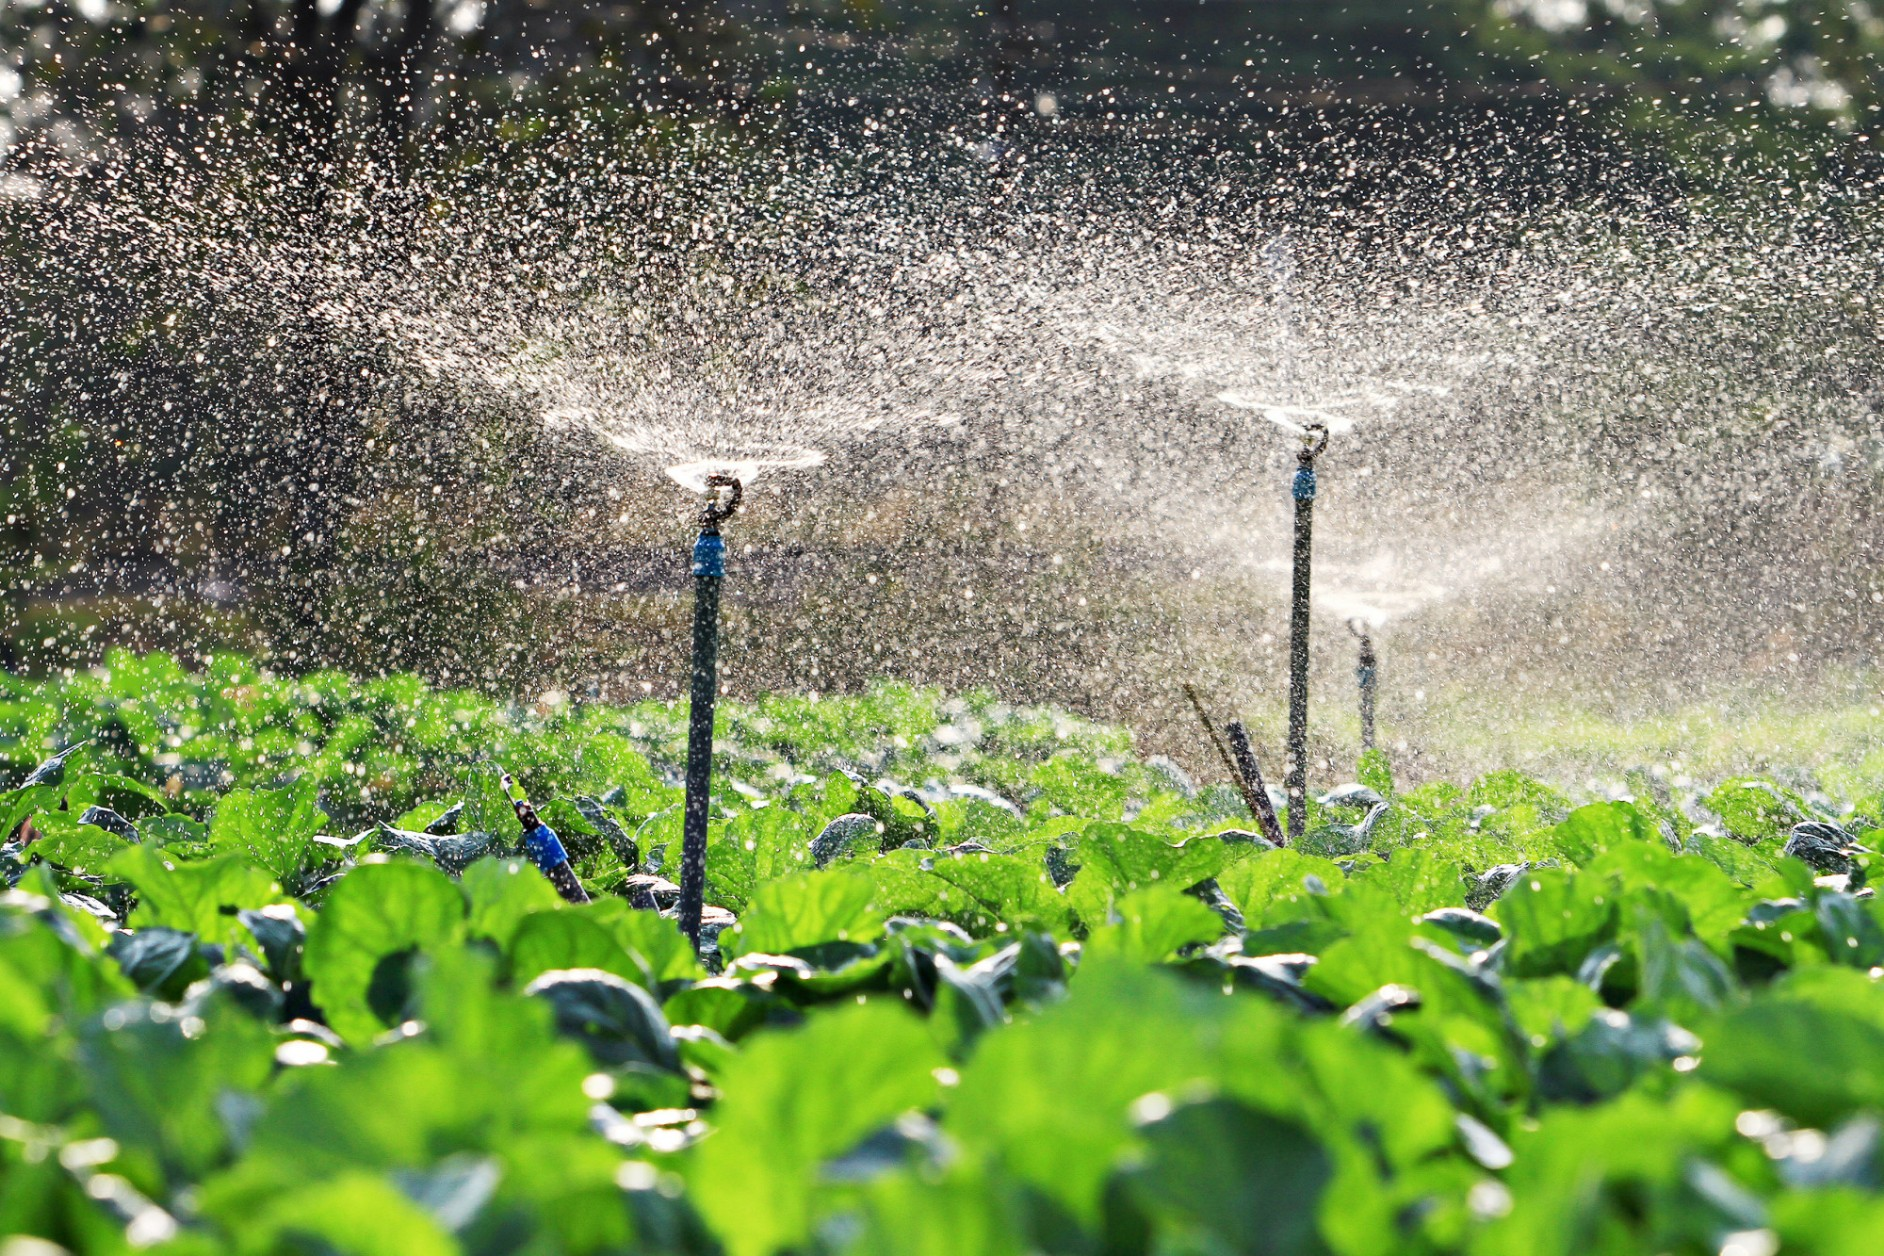
\includegraphics[width=\textwidth, height=3.8cm]{images/irrigation.jpg}
			\caption{Irrigation}
		\end{subfigure}
		\hfill
		\begin{subfigure}[b]{0.3\textwidth}
			\centering
			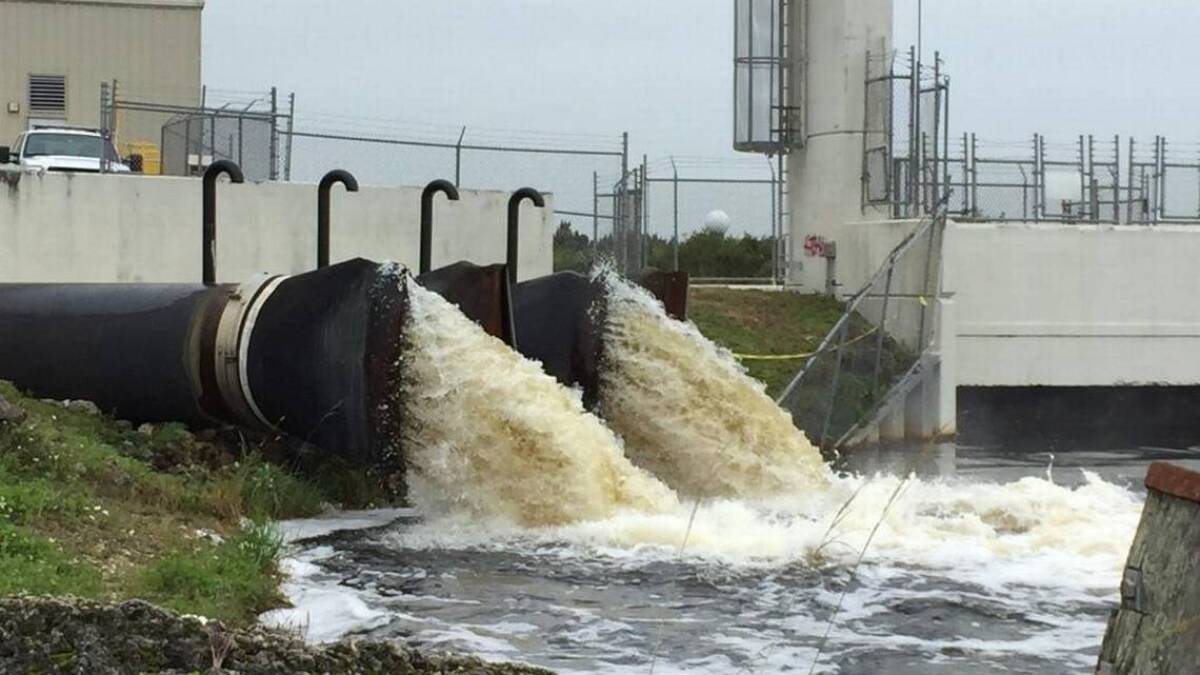
\includegraphics[width=\textwidth, height=3.8cm]{images/flood_control.jpeg}
			\caption{Flood control}
		\end{subfigure}
		\hfill
		\begin{subfigure}[b]{0.3\textwidth}
			\centering
			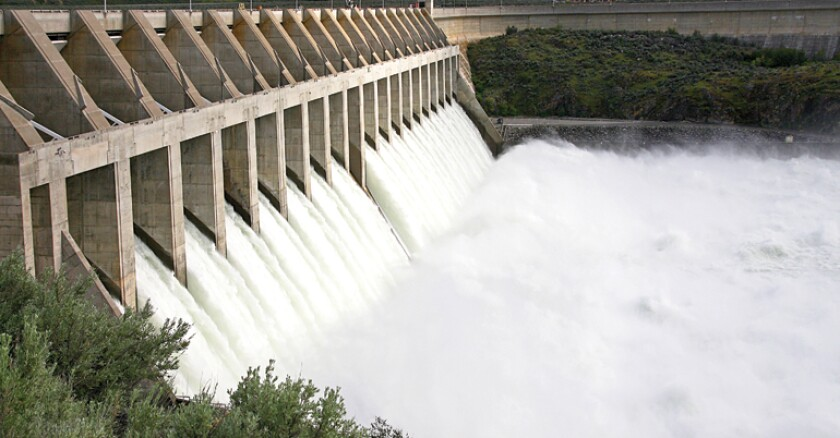
\includegraphics[width=\textwidth, height=3.8cm]{images/hydro_gen.jpeg}
			\caption{Hydropower generation}
		\end{subfigure}
		
	\end{figure}
	\begin{block}{\textcolor{myNewColorB}{\textbf{Challenges}}}
	Non-linearities, high stochasticity, and complex water resource patterns.
	\end{block}
	
\end{frame}

\begin{frame}
	\frametitle{The Importance of Hydrological Forecasting}
	\begin{block}{}
	Understanding hydrological processes has become increasingly critical in the field of natural resource management, anticipation capacity of extreme hydrological events such as droughts and heavy rainfall.
	\end{block}
	\begin{figure}
		\centering
		\begin{subfigure}[b]{0.45\textwidth}
			\centering
			\includegraphics[width=\textwidth, height=4cm]{images/drought.jpg}
			\caption{Drought Condition}
		\end{subfigure}
		\hfill
		\begin{subfigure}[b]{0.45\textwidth}
			\centering
			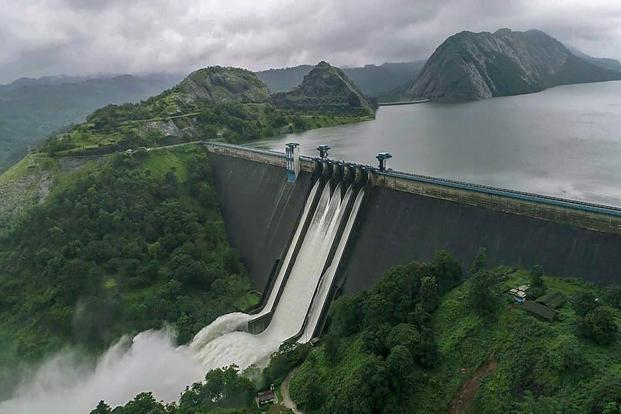
\includegraphics[width=\textwidth, height=4cm]{images/full_dam.jpg}
			\caption{Full Dam}
		\end{subfigure}
	\end{figure}
	
\end{frame}

\begin{frame}{Problem Statement and Research Question}
	\begin{block}{}
	\begin{itemize}
		\item Physically driven models for water resource forecasting are complex and require extensive parameter knowledge, limiting their practicality \cite{Yaseen2018, HKASHANI2016340}.
		\item Data-driven models, such as autoregressive (AR) models, struggle to capture nonlinearities in water resources time series \cite{10.2166/wst.2020.369}.
		\item Neural networks (ANNs, RNNs) improve on nonlinearity, but face overfitting, gradient vanishing and exploding, limiting ability to capture long-term dependencies \cite{Abdollahi2017, Shiau2016, KHAN2020125380}.
		\item LSTM networks overcome these issues, but lack uncertainty quantification, crucial for decision-making in hydrological forecasting \cite{lakshminarayanan2017simple, gal2016dropout}.
		\item Gaussian Processes (GPs) provide uncertainty and handle nonlinearities, but scaling to multi-task forecasting remains a challenge \cite{QUILTY2020104718, NIU2021102562,bruinsma2020scalable}.
	\end{itemize}
	\end{block}
	\begin{block}{\textbf{Research Question}}
		How to develop a joint probabilistic prediction model for multiple hydrological series associated with electricity generation, that describes the randomness of the forecast, is scalable, and utilizes task correlations to improve performance?
	\end{block}
\end{frame}


\section{Objectives}

\begin{frame}{Objectives}
	\begin{block}{\textbf{General Objective}}
			Develop a stochastic forecasting model for making multiple simultaneous predictions of hydrological time series. This model will take advantage of cross-correlations among the tasks to improve performance, while maintaining scalability for short-term horizons.
	\end{block}
	
	\begin{block}{\textbf{Specific Objectives}}
			
			\begin{itemize}
			\item Develop a model that allows the forecasting of hydrological time series, properly quantifying the uncertainty associated with each value within the prediction horizons.
			\item  Design a multi-task forecasting methodology that captures and models cross-correlations between hydrological time series, to improve forecast accuracy within forecast horizons.
			\item Develop a multi-task prediction methodology that handles data constraints across reservoirs while maintaining high forecasting performance as measured by probabilistic metrics.
		\end{itemize}
	\end{block}
\end{frame}

\section{The Dataset}

\begin{frame}{Problem Setting}
	We model hydrological time series using observed resource vectors. At each time step \( n \), the vector \(\mathbf{v}_n \in \mathbb{R}^D\) represents resources across \(D\) outputs.
	
	The input vector \(\mathbf{x}_n\) for the model is constructed from the resource vectors from time \( n \) back to \( n-T+1 \):
	
	\begin{equation*}
		\mathbf{x}_n = \begin{bmatrix} 
			\mathbf{v}_{n}^\top \\ 
			\mathbf{v}_{n-1}^\top \\ 
			\vdots \\ 
			\mathbf{v}_{n-T+1}^\top 
		\end{bmatrix} \in \mathcal{X}
	\end{equation*}
	
	Here, \( T \) is the model order and \( H \) is the prediction horizon and \( \mathcal{X}\subset \mathbb{R}^{DT} \) represents the input space.
	
	\vspace{10pt}
	
	The target output vector \(\mathbf{y}_n\) is:
	
	\begin{equation*}
		\mathbf{y}_n = \mathbf{v}_{n+H} \in \mathbb{R}^{D}
	\end{equation*}
	
	We build a dataset \(\mathcal{D} = \{\mathbf{x}_n, \mathbf{y}_n\}_{n=1}^N  = \{\mathbf{X}, \mathbf{y}\}\), comprising \( N \) input-output pairs.
\end{frame}


\begin{frame}{Reservoir Locations and Dataset Overview}
	\begin{columns}[T] % Top alignment
		\begin{column}{0.45\textwidth}
			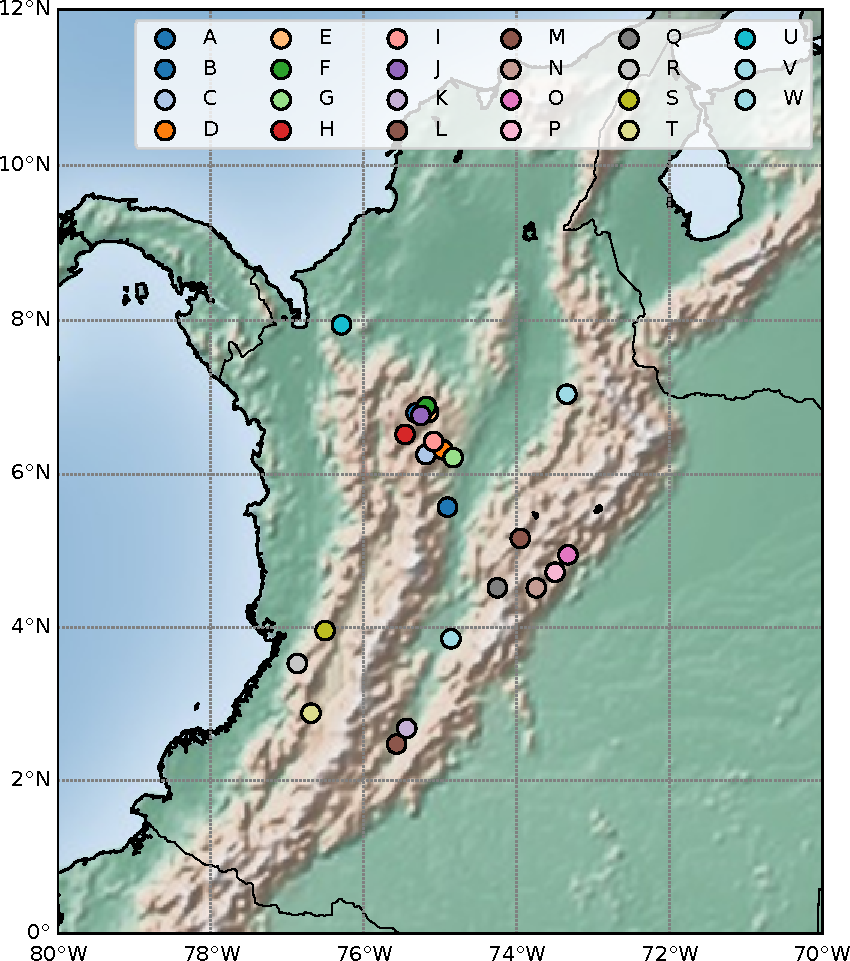
\includegraphics[width=\linewidth]{images/colombiamap.pdf}
		
		\end{column}
		\begin{column}{0.55\textwidth}
			\justifying % Justifies text
			\begin{block}{}
			The hydrological forecasting task utilizes daily streamflow data from 23 Colombian reservoirs from January 1, 2010, to February 28, 2022.
			\end{block}
			\begin{figure}[htbp]
				\centering
				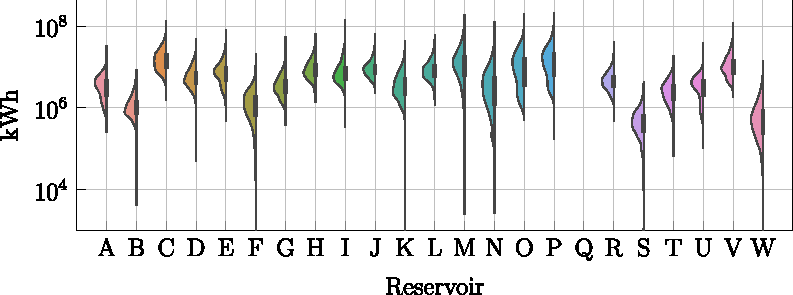
\includegraphics[width=\textwidth]{images/ct_violinplot.pdf}
			\end{figure}
			\begin{block}{}
			Although volumetric measurements are recorded, they are reported in kilowatt-hours (kWh) by the hydroelectric power plants.
			\end{block}
		\end{column}
	\end{columns}
\end{frame}

\subsection{Methodoly}
\begin{frame}{Methodology}
	\justifying
	\begin{block}{\textbf{Performance Metrics}}
	\begin{itemize}
		\item Mean Squared Error (MSE)
		\item Mean Standardized Log Loss (MSLL)
		\item Continuous Ranked Probability Score (CRPS)
		\item Negative Log Predictive Density (NLPD)
	\end{itemize}
	\end{block}
	
	\begin{block}{\textbf{Gaussian Process Models}}
	\begin{itemize}
		\item Start with a single-output GP for stochastic regression.
		\item Extend to multi-output GPs, capturing dependencies across multiple reservoirs.
		\item Introduce Chained Correlated Gaussian Processes to handle non-Gaussian likelihoods.
	\end{itemize}
	\end{block}
\end{frame}

\section{Gaussian Process Regression: Bayesian Non-Parametric Model}

\subsection{Mathematical Framework}

\begin{frame}{Gaussian Process (GP) Framework}
	In a GP framework, the function $\bm{f}(\cdot)$ maps inputs $\bm{x}_n$ to outputs $\bm{y}_n$. Adding i.i.d. Gaussian noise $\bm{\epsilon}$, the model becomes:
	
	\[
	\bm{y}_n = \bm{f}(\bm{x}_n) + \bm{\epsilon}
	\]
	
	For test inputs $\mathbf{X}_*$, the joint distribution of training outputs $\mathbf{y}$ and test outputs $\mathbf{f}_*$ is:
	
	\[
	\left[ \begin{array}{c}
		\mathbf{y}\\
		\mathbf{f_*}\\
	\end{array}
	\right] \sim \mathcal{N} \left( \bm{0}, \left[
	\begin{array}{cc}
		\mathbf{K}_y & \mathbf{K}_* \\
		\mathbf{K}_*^\top & \mathbf{K}_{**}
	\end{array}\right] \right)
	\]
	
	The posterior distribution for test points is:
	
	\[
	\mathbf{f}_* | \mathbf{X}_*, \mathcal{D} \sim \mathcal{N}(\mathbf{K}_*^\top \mathbf{K}_y^{-1} \mathbf{y}, \mathbf{K}_{**} - \mathbf{K}_*^\top \mathbf{K}_y^{-1} \mathbf{K}_*)
	\]
	
	\begin{itemize}
		\item $\mathbf{K}_y = \mathbf{K} + \Sigma_\epsilon$, where $\mathbf{K} \in \mathbb{R}^{ND \times ND}$ is the covariance matrix for the train set and $\Sigma_\epsilon$ contains task-wise noise.
		
		\item $\mathbf{K}_{**} \in \mathbb{R}^{N_* D \times N_* D}$ is the covariance matrix for the test set.
		
		\item $\mathbf{K}_* \in \mathbb{R}^{ND \times N_* D}$ represents the cross-covariance matrix between the training and test points.
	\end{itemize}
	
\end{frame}


\begin{frame}{The Marginal Log-likelihood}
	\justifying
	The prediction performance achieved by the conditional distribution is influenced by the selected parameter set $\bm{\theta}$ and the observation noise matrix $\Sigma_\epsilon$. These parameters are determined by maximizing the marginal log-likelihood, where the marginal likelihood $p(\mathbf{y})$ follows a Gaussian distribution:
	
	\[
	p(\mathbf{y}) = \mathcal{N}(\mathbf{y} \mid \bm{0}, \mathbf{K}_y)
	\]
	
	The optimization problem is defined as:
	
	\begin{equation*}\label{eq:sogp_nlml_opt}
		\begin{aligned}
			\{\bm{\theta}_{\text{opt}}, {\Sigma_\epsilon}_{\text{opt}}\} &= \underset{\bm{\theta}, \Sigma_\epsilon}{\arg\max} \quad \ln p(\mathbf{y}) \\
			&= \underset{\bm{\theta}, \Sigma_\epsilon}{\arg\min} \quad \frac{1}{2} \mathbf{y}^\top \mathbf{K}_y^{-1} \mathbf{y} + \frac{1}{2} \ln \lvert \mathbf{K}_y \rvert + \frac{ND}{2} \ln 2\pi
		\end{aligned}
	\end{equation*}
	
	\vspace{3mm}
	\justifying
	However, the main challenge lies in the computational complexity of $\mathcal{O}(N^3D^3)$ and the storage demand of $\mathcal{O}(N^2D^2)$ due to the need to invert the matrix $\mathbf{K}_y$.
\end{frame}

\begin{frame}{Variational Inference and Sparse Variational GPs (SVGPs)}
	We introduce $M \ll N$ inducing points $Z$, with inducing variables $\mathbf{u} \in \mathbb{R}^{MD}$ to reduce computational complexity. The joint distribution becomes:
	\[
	\begin{array}{rcl}
		\left[ \begin{array}{c}
			\mathbf{u}\\
			\mathbf{f}\\
		\end{array}
		\right]
		\sim
		\mathcal{N} \left(
		\begin{array}{c}
			\mathbf{0}\\
		\end{array},
		\left[ \begin{array}{cc}
			\mathbf{K}_{uu} & \mathbf{K}_{uf}\\
			\mathbf{K}_{uf}^\top & \mathbf{K}\\
		\end{array}
		\right] \right)
	\end{array}
	\]
	Where $\mathbf{K}_{uu} \in \mathbb{R}^{MD \times MD}$, and $\mathbf{K}_{uf} \in \mathbb{R}^{MD \times ND}$. The posterior distribution uses the variational approximation $q(\mathbf{u}) = \mathcal{N}(\boldsymbol{\mu}, \mathbf{S})$. Now we maximizing the Evidence Lower Bound (ELBO):
	\begin{equation*}
		\mathcal{L} = \sum_{d=1}^D \sum_{n=1}^N \mathbb{E}_{q(f_d(\mathbf{x}_n))}\{\ln p(y_{dn} \mid f_d(\mathbf{x}_n))\} - \sum_{d=1}^D \text{KL}\{q(\mathbf{u}_d) \parallel p(\mathbf{u}_d)\} \leq \ln p(\mathbf{y})
	\end{equation*}
	where $f_d(\mathbf{x}_n)$ represents the $d$-th latent function value at input $\mathbf{x}_n$, and $y_{dn}$ is the corresponding observed value. This reduces the complexity to $\mathcal{O}(NM^2D^3)$. For predictions at new points $\mathbf{x}_*$, we add noise in $\Sigma_\epsilon$ to $q(\mathbf{f}_*) = \int p(\mathbf{f}_* \mid \mathbf{u}) q(\mathbf{u}) d\mathbf{u}$.
\end{frame}

\begin{frame}{Model Setup}
	The GP covariance is factorized into two kernels: $k_{\mathcal{X}}$ for input correlations and $k_{D}$ for task correlations:
	\[
	k\left((\bm{x}, d), (\bm{x}', d')\right) = k_{\mathcal{X}}\left(\bm{x}, \bm{x}' \mid \bm{\Theta}_d \right) k_{D}\left(d, d' \mid \sigma_d \right),
	\]
	with:
	\[
	k_{\mathcal{X}}\left(\bm{x}, \bm{x}'\right) = \exp\left(-\frac{1}{2}(\bm{x} - \bm{x}')^\top \bm{\Theta}_d^{-2} (\bm{x} - \bm{x}')\right),
	\]
	\[
	k_{D}(d, d') = \sigma^2_d \delta_{d, d'},
	\]
	where $\delta_{d, d'}$ is the Kronecker delta, $\bm{\Theta}_d$ is the lengthscale matrix, and $\sigma^2_d$ is the output scale. This reduces complexity to $\mathcal{O}(NM^2D)$ by avoiding explicit task correlations.
\end{frame}



\subsection{Results and Discussions}

\begin{frame}{Tuning M and T}
 	\begin{figure}[htbp]
	 	% \centering
	 	\setlength\figurewidth{0.5\textwidth} 
	 	\setlength\figureheight{0.5\textwidth}
 		\subfloat[MSLL ($\times10^{-2}$)]{% This file was created with tikzplotlib v0.10.1.
\begin{tikzpicture}

\definecolor{darkgray176}{RGB}{176,176,176}
\definecolor{darkslategray38}{RGB}{38,38,38}

\begin{axis}[
width=\figurewidth,
height=\figureheight,
% colorbar,
% colorbar style={ylabel={}},
colormap={mymap}{[1pt]
  rgb(0pt)=(1,1,0.850980392156863);
  rgb(1pt)=(0.929411764705882,0.972549019607843,0.694117647058824);
  rgb(2pt)=(0.780392156862745,0.913725490196078,0.705882352941177);
  rgb(3pt)=(0.498039215686275,0.803921568627451,0.733333333333333);
  rgb(4pt)=(0.254901960784314,0.713725490196078,0.768627450980392);
  rgb(5pt)=(0.113725490196078,0.568627450980392,0.752941176470588);
  rgb(6pt)=(0.133333333333333,0.368627450980392,0.658823529411765);
  rgb(7pt)=(0.145098039215686,0.203921568627451,0.580392156862745);
  rgb(8pt)=(0.0313725490196078,0.113725490196078,0.345098039215686)
},
point meta max=-0.0763556642639684,
point meta min=-0.452207182874033,
% tick align=outside,
tick pos=left,
% title={MSLL},
xlabel={$T$},
x grid style={darkgray176},
xmin=0, xmax=7,
xtick style={color=black},
xtick={0.5,1.5,2.5,3.5,4.5,5.5,6.5},
xticklabels={1, 2,  3, 7, 14, 21, 30},
%ylabel={$M$},
yticklabel style={rotate=0.0, font=\footnotesize},
xticklabel style={rotate=0.0, font=\footnotesize},
xtick style={draw=none},
ytick style={draw=none},
y dir=reverse,
y grid style={darkgray176},
ymin=0, ymax=5,
ytick style={color=black},
ytick={0.5,1.5,2.5,3.5,4.5},
yticklabels={}
]
\addplot graphics [includegraphics cmd=\pgfimage,xmin=0, xmax=7, ymin=5, ymax=0] {chp_sogp/figures/gs_msll-000.png};
\draw[red, thick] (axis cs:0.01,3) rectangle (axis cs:1.01,4);

\draw (axis cs:0.5,0.5) node[
  scale=0.5,
  text=white,
  rotate=0.0
]{$-42.51$};
\draw (axis cs:1.5,0.5) node[
  scale=0.5,
  text=white,
  rotate=0.0
]{$-38.50$};
\draw (axis cs:2.5,0.5) node[
  scale=0.5,
  text=white,
  rotate=0.0
]{$-34.76$};
\draw (axis cs:3.5,0.5) node[
  scale=0.5,
  text=white,
  rotate=0.0
]{$-31.20$};
\draw (axis cs:4.5,0.5) node[
  scale=0.5,
  text=darkslategray38,
  rotate=0.0
]{$-7.64$};
\draw (axis cs:5.5,0.5) node[
  scale=0.5,
  text=darkslategray38,
  rotate=0.0
]{$-7.65$};
\draw (axis cs:6.5,0.5) node[
  scale=0.5,
  text=darkslategray38,
  rotate=0.0
]{$-7.65$};
\draw (axis cs:0.5,1.5) node[
  scale=0.5,
  text=white,
  rotate=0.0
]{$-44.49$};
\draw (axis cs:1.5,1.5) node[
  scale=0.5,
  text=white,
  rotate=0.0
]{$-39.07$};
\draw (axis cs:2.5,1.5) node[
  scale=0.5,
  text=white,
  rotate=0.0
]{$-37.02$};
\draw (axis cs:3.5,1.5) node[
  scale=0.5,
  text=white,
  rotate=0.0
]{$-32.22$};
\draw (axis cs:4.5,1.5) node[
  scale=0.5,
  text=darkslategray38,
  rotate=0.0
]{$-7.65$};
\draw (axis cs:5.5,1.5) node[
  scale=0.5,
  text=darkslategray38,
  rotate=0.0
]{$-17.78$};
\draw (axis cs:6.5,1.5) node[
  scale=0.5,
  text=darkslategray38,
  rotate=0.0
]{$-9.04$};
\draw (axis cs:0.5,2.5) node[
  scale=0.5,
  text=white,
  rotate=0.0
]{$-45.15$};
\draw (axis cs:1.5,2.5) node[
  scale=0.5,
  text=white,
  rotate=0.0
]{$-40.89$};
\draw (axis cs:2.5,2.5) node[
  scale=0.5,
  text=white,
  rotate=0.0
]{$-37.00$};
\draw (axis cs:3.5,2.5) node[
  scale=0.5,
  text=white,
  rotate=0.0
]{$-31.71$};
\draw (axis cs:4.5,2.5) node[
  scale=0.5,
  text=white,
  rotate=0.0
]{$-25.77$};
\draw (axis cs:5.5,2.5) node[
  scale=0.5,
  text=darkslategray38,
  rotate=0.0
]{$-17.76$};
\draw (axis cs:6.5,2.5) node[
  scale=0.5,
  text=darkslategray38,
  rotate=0.0
]{$-11.59$};
\draw (axis cs:0.5,3.5) node[
  scale=0.5,
  text=white,
  rotate=0.0
]{$-45.22$};
\draw (axis cs:1.5,3.5) node[
  scale=0.5,
  text=white,
  rotate=0.0
]{$-40.90$};
\draw (axis cs:2.5,3.5) node[
  scale=0.5,
  text=white,
  rotate=0.0
]{$-36.92$};
\draw (axis cs:3.5,3.5) node[
  scale=0.5,
  text=white,
  rotate=0.0
]{$-32.50$};
\draw (axis cs:4.5,3.5) node[
  scale=0.5,
  text=white,
  rotate=0.0
]{$-25.67$};
\draw (axis cs:5.5,3.5) node[
  scale=0.5,
  text=white,
  rotate=0.0
]{$-19.38$};
\draw (axis cs:6.5,3.5) node[
  scale=0.5,
  text=darkslategray38,
  rotate=0.0
]{$-10.44$};
\draw (axis cs:0.5,4.5) node[
  scale=0.5,
  text=white,
  rotate=0.0
]{$-44.97$};
\draw (axis cs:1.5,4.5) node[
  scale=0.5,
  text=white,
  rotate=0.0
]{$-41.16$};
\draw (axis cs:2.5,4.5) node[
  scale=0.5,
  text=white,
  rotate=0.0
]{$-37.07$};
\draw (axis cs:3.5,4.5) node[
  scale=0.5,
  text=white,
  rotate=0.0
]{$-32.52$};
\draw (axis cs:4.5,4.5) node[
  scale=0.5,
  text=white,
  rotate=0.0
]{$-26.59$};
\draw (axis cs:5.5,4.5) node[
  scale=0.5,
  text=white,
  rotate=0.0
]{$-19.45$};
\draw (axis cs:6.5,4.5) node[
  scale=0.5,
  text=darkslategray38,
  rotate=0.0
]{$-13.15$};
\end{axis}

\end{tikzpicture}
}\hspace{-1em}
 		\subfloat[MSE ($\times10^{-1}$)]{% This file was created with tikzplotlib v0.10.1.
\begin{tikzpicture}

\definecolor{darkgray176}{RGB}{176,176,176}
\definecolor{darkslategray38}{RGB}{38,38,38}

\begin{axis}[
width=\figurewidth,
height=\figureheight,
% colorbar,
% colorbar style={ylabel={}},
colormap={mymap}{[1pt]
  rgb(0pt)=(1,1,0.850980392156863);
  rgb(1pt)=(0.929411764705882,0.972549019607843,0.694117647058824);
  rgb(2pt)=(0.780392156862745,0.913725490196078,0.705882352941177);
  rgb(3pt)=(0.498039215686275,0.803921568627451,0.733333333333333);
  rgb(4pt)=(0.254901960784314,0.713725490196078,0.768627450980392);
  rgb(5pt)=(0.113725490196078,0.568627450980392,0.752941176470588);
  rgb(6pt)=(0.133333333333333,0.368627450980392,0.658823529411765);
  rgb(7pt)=(0.145098039215686,0.203921568627451,0.580392156862745);
  rgb(8pt)=(0.0313725490196078,0.113725490196078,0.345098039215686)
},
point meta max=0.798073230683677,
point meta min=0.451356129772609,
% tick align=outside,
tick pos=left,
% title={MSE},
xlabel={$T$},
x grid style={darkgray176},
xmin=0, xmax=7,
xtick style={color=black},
xtick={0.5,1.5,2.5,3.5,4.5,5.5,6.5},
xticklabels={1, 2,  3, 7, 14, 21, 30},
xticklabel style={rotate=0.0, font=\footnotesize},
xtick style={draw=none},
ytick style={draw=none},
y dir=reverse,
y grid style={darkgray176},
ymin=0, ymax=5,
ytick style={color=black},
ytick={0.5,1.5,2.5,3.5,4.5},
yticklabels={}
]
\addplot graphics [includegraphics cmd=\pgfimage,xmin=0, xmax=7, ymin=5, ymax=0] {chp_sogp/figures/gs_mse-000.png};
\draw (axis cs:0.5,0.5) node[
  scale=0.5,
  text=white,
  rotate=0.0
]{$4.69$};
\draw (axis cs:1.5,0.5) node[
  scale=0.5,
  text=white,
  rotate=0.0
]{$4.68$};
\draw (axis cs:2.5,0.5) node[
  scale=0.5,
  text=white,
  rotate=0.0
]{$4.92$};
\draw (axis cs:3.5,0.5) node[
  scale=0.5,
  text=white,
  rotate=0.0
]{$5.42$};
\draw (axis cs:4.5,0.5) node[
  scale=0.5,
  text=darkslategray38,
  rotate=0.0
]{$7.80$};
\draw (axis cs:5.5,0.5) node[
  scale=0.5,
  text=darkslategray38,
  rotate=0.0
]{$7.85$};
\draw (axis cs:6.5,0.5) node[
  scale=0.5,
  text=darkslategray38,
  rotate=0.0
]{$7.98$};
\draw (axis cs:0.5,1.5) node[
  scale=0.5,
  text=white,
  rotate=0.0
]{$4.58$};
\draw (axis cs:1.5,1.5) node[
  scale=0.5,
  text=white,
  rotate=0.0
]{$4.69$};
\draw (axis cs:2.5,1.5) node[
  scale=0.5,
  text=white,
  rotate=0.0
]{$4.79$};
\draw (axis cs:3.5,1.5) node[
  scale=0.5,
  text=white,
  rotate=0.0
]{$5.08$};
\draw (axis cs:4.5,1.5) node[
  scale=0.5,
  text=darkslategray38,
  rotate=0.0
]{$7.80$};
\draw (axis cs:5.5,1.5) node[
  scale=0.5,
  text=darkslategray38,
  rotate=0.0
]{$7.85$};
\draw (axis cs:6.5,1.5) node[
  scale=0.5,
  text=darkslategray38,
  rotate=0.0
]{$7.98$};
\draw (axis cs:0.5,2.5) node[
  scale=0.5,
  text=white,
  rotate=0.0
]{$4.53$};
\draw (axis cs:1.5,2.5) node[
  scale=0.5,
  text=white,
  rotate=0.0
]{$4.59$};
\draw (axis cs:2.5,2.5) node[
  scale=0.5,
  text=white,
  rotate=0.0
]{$4.75$};
\draw (axis cs:3.5,2.5) node[
  scale=0.5,
  text=white,
  rotate=0.0
]{$5.10$};
\draw (axis cs:4.5,2.5) node[
  scale=0.5,
  text=white,
  rotate=0.0
]{$5.86$};
\draw (axis cs:5.5,2.5) node[
  scale=0.5,
  text=darkslategray38,
  rotate=0.0
]{$7.85$};
\draw (axis cs:6.5,2.5) node[
  scale=0.5,
  text=darkslategray38,
  rotate=0.0
]{$7.98$};
\draw (axis cs:0.5,3.5) node[
  scale=0.5,
  text=white,
  rotate=0.0
]{$4.51$};
\draw (axis cs:1.5,3.5) node[
  scale=0.5,
  text=white,
  rotate=0.0
]{$4.60$};
\draw (axis cs:2.5,3.5) node[
  scale=0.5,
  text=white,
  rotate=0.0
]{$4.68$};
\draw (axis cs:3.5,3.5) node[
  scale=0.5,
  text=white,
  rotate=0.0
]{$5.04$};
\draw (axis cs:4.5,3.5) node[
  scale=0.5,
  text=white,
  rotate=0.0
]{$5.66$};
\draw (axis cs:5.5,3.5) node[
  scale=0.5,
  text=white,
  rotate=0.0
]{$6.24$};
\draw (axis cs:6.5,3.5) node[
  scale=0.5,
  text=darkslategray38,
  rotate=0.0
]{$7.98$};
\draw (axis cs:0.5,4.5) node[
  scale=0.5,
  text=white,
  rotate=0.0
]{$5.01$};
\draw (axis cs:1.5,4.5) node[
  scale=0.5,
  text=white,
  rotate=0.0
]{$4.60$};
\draw (axis cs:2.5,4.5) node[
  scale=0.5,
  text=white,
  rotate=0.0
]{$4.66$};
\draw (axis cs:3.5,4.5) node[
  scale=0.5,
  text=white,
  rotate=0.0
]{$4.99$};
\draw (axis cs:4.5,4.5) node[
  scale=0.5,
  text=white,
  rotate=0.0
]{$5.60$};
\draw (axis cs:5.5,4.5) node[
  scale=0.5,
  text=white,
  rotate=0.0
]{$6.20$};
\draw (axis cs:6.5,4.5) node[
  scale=0.5,
  text=darkslategray38,
  rotate=0.0
]{$7.98$};
\end{axis}

\end{tikzpicture}
}
	\end{figure}
	Grid search average values for tuning the model order $T$ and the number of inducing points $M$. The optimal settings are $M=64$ and $T=1$
\end{frame}

\begin{frame}{Reservoir-Wise Output Scales and Noise Variance}
	
	\begin{figure}[htbp]
		% \centering
	 	\setlength\figurewidth{0.52\textwidth} 
		\setlength\figureheight{0.5\textwidth}
		\subfloat[Output scales]{% This file was created with tikzplotlib v0.10.1.
\begin{tikzpicture}
	\setlength{\abovecaptionskip}{-1em}   % Adjust to reduce space above caption
	\setlength{\belowcaptionskip}{-1em}   % Adjust to reduce space below caption
	
	\definecolor{darkgray176}{RGB}{176,176,176}
	\definecolor{darkslategray38}{RGB}{38,38,38}
	
	\begin{axis}[
		width=\figurewidth, % Adjust this value to control figure width
		height=\figureheight, % Adjust this value to control figure height
		colorbar,
		colorbar style={ylabel={}, width=0.05\figurewidth}, % Adjust colorbar width
		colormap/viridis,
		point meta max=0.303282008679354,
		point meta min=0.0135929814440097,
		tick align=outside,
		tick pos=left,
		x grid style={darkgray176},
		xmin=0, xmax=10,
		xtick style={color=black},
		xtick={0.5,1.5,2.5,3.5,4.5,5.5,6.5,7.5,8.5,9.5},
		xticklabels={1, 2, 3, 4, 5, 6, 7, 14, 21, 30},
		xticklabel style={rotate=0.0, font=\tiny, yshift=1ex},
		xlabel={Horizon ($H$)},
		y dir=reverse,
		y grid style={darkgray176},
		ymin=0, ymax=23,
		ytick style={color=black},
		ylabel={Reservoir},
		ytick={0.5,2.5,4.5,6.5,8.5,10.5,12.5,14.5,16.5,18.5,20.5,22.5},
		yticklabel style={rotate=0.0, font=\tiny},
		xtick style={draw=none}, % Hide x-tick marks
		ytick style={draw=none}, % Hide y-tick marks
		yticklabels={A,C,E,G,I,K,M,O,Q,S,U,W},
		]
		\addplot graphics [includegraphics cmd=\pgfimage,xmin=0, xmax=10, ymin=23, ymax=0] {chp_sogp/figures/output_scale_matrix-000.png};
		
	\end{axis}
	
\end{tikzpicture}
}\hspace{-1em}
		\subfloat[Noise variances]{% This file was created with tikzplotlib v0.10.1.
\begin{tikzpicture}
	\setlength{\abovecaptionskip}{-5em}   % Adjust to reduce space above caption
	\setlength{\belowcaptionskip}{-5em}   % Adjust to reduce space below caption
	
	\definecolor{darkgray176}{RGB}{176,176,176}
	\definecolor{darkslategray38}{RGB}{38,38,38}
	
	\begin{axis}[
		width=\figurewidth, % Adjust this value to control figure width
		height=\figureheight, % Adjust this value to control figure height
		colorbar,
		colorbar style={ylabel={}, width=0.05\figurewidth}, % Adjust colorbar width
		colormap/viridis,
		point meta max=0.926209144036932,
		point meta min=0.00152376959235976,
		tick pos=left,
		x grid style={darkgray176},
		xmin=0, xmax=10,
		xtick style={color=black},
		xtick={0.5,1.5,2.5,3.5,4.5,5.5,6.5,7.5,8.5,9.5},
		xticklabels={1, 2, 3, 4, 5, 6, 7, 14, 21, 30},
		xticklabel style={rotate=0.0, font=\tiny, yshift=-1ex},
		xlabel={Horizon ($H$)},
		y dir=reverse,
		y grid style={darkgray176},
		ymin=0, ymax=23,
		ytick style={color=black},
		ytick={0.5,1.5,2.5,3.5,4.5,5.5,6.5,7.5,8.5,9.5,10.5,11.5,12.5,13.5,14.5,15.5,16.5,17.5,18.5,19.5,20.5,21.5,22.5},
		yticklabels={}
		]
		\addplot graphics [includegraphics cmd=\pgfimage,xmin=0, xmax=10, ymin=23, ymax=0] {chp_sogp/figures/noise_variance_matrix-000.png};
		
	\end{axis}
	
\end{tikzpicture}
}
	\end{figure}
	Output scales $\sigma^2_d$ and noise variance $\Sigma_\epsilon$ tuned for each horizon and reservoir. Longer horizons generally show smaller output scales and higher noise variance.
\end{frame}


\begin{frame}{Lengthscale Analysis}
	\begin{figure}[htbp]
		\centering
		\tiny
		\setlength\figurewidth{0.4\columnwidth} 
		\setlength\figureheight{0.42\columnwidth}
		\subfloat[$H=1.$]{% This file was created with tikzplotlib v0.10.1.
\begin{tikzpicture}

\definecolor{darkgray176}{RGB}{176,176,176}

\begin{axis}[
width=\figurewidth,
height=\figureheight,
% colorbar,
ylabel={Target Reservoir},
xlabel={Input Reservoir},
colorbar style={ylabel={}},
colormap/viridis,
point meta max=6,
point meta min=2,
% tick align=outside,
tick pos=left,
x grid style={darkgray176},
xmin=0, xmax=23,
xtick style={color=black},
xtick={0.5,2.5,4.5,6.5,8.5,10.5,12.5,14.5,16.5,18.5,20.5,22.5},
xticklabel style={rotate=0.0, font=\tiny},
xticklabels={A,C,E,G,I,K,M,O,Q,S,U,W},
y dir=reverse,
y grid style={darkgray176},
ymin=0, ymax=23,
ytick style={color=black},
ytick={0.5,2.5,4.5,6.5,8.5,10.5,12.5,14.5,16.5,18.5,20.5,22.5},
xtick style={draw=none},
ytick style={draw=none},
yticklabel style={rotate=0.0, font=\tiny},
yticklabels={A,C,E,G,I,K,M,O,Q,S,U,W},
%   AMANI,
]
\addplot graphics [includegraphics cmd=\pgfimage,xmin=0, xmax=23, ymin=23, ymax=0] {chp_sogp/figures/lengthscalematrix1-000.png};
\end{axis}

\end{tikzpicture}
}\hspace{-1.3em}
		\subfloat[$H=14.$]{% This file was created with tikzplotlib v0.10.1.
\begin{tikzpicture}

\definecolor{darkgray176}{RGB}{176,176,176}

\begin{axis}[
width=\figurewidth,
height=\figureheight,
% colorbar,
colorbar style={ylabel={}},
colormap/viridis,
point meta max=6,
point meta min=2,
xlabel={Input Reservoir},
% tick align=outside,
tick pos=left,
x grid style={darkgray176},
xmin=0, xmax=23,
xtick style={color=black},
xtick={0.5,2.5,4.5,6.5,8.5,10.5,12.5,14.5,16.5,18.5,20.5,22.5},
xticklabel style={rotate=0.0, font=\tiny},
xticklabels={A,C,E,G,I,K,M,O,Q,S,U,W},
y dir=reverse,
y grid style={darkgray176},
ymin=0, ymax=23,
ytick style={color=black},
ytick={0.5,1.5,2.5,3.5,4.5,5.5,6.5,7.5,8.5,9.5,10.5,11.5,12.5,13.5,14.5,15.5,16.5,17.5,18.5,19.5,20.5,21.5,22.5},
yticklabels={}
]
\addplot graphics [includegraphics cmd=\pgfimage,xmin=0, xmax=23, ymin=23, ymax=0] {chp_sogp/figures/lengthscalematrix14-000.png};
\end{axis}

\end{tikzpicture}
}\hspace{-1.3em}
		\subfloat[$H=30.$]{% This file was created with tikzplotlib v0.10.1.
\begin{tikzpicture}

\definecolor{darkgray176}{RGB}{176,176,176}

\begin{axis}[
width=\figurewidth,
height=\figureheight,
colorbar,
colorbar style={ylabel={$\Delta_{dl}$}, ylabel style={rotate=-90}, at={(1.03, 1)}},
colormap/viridis,
point meta max=6,
point meta min=2,
% tick align=outside,
xlabel={Input Reservoir},
tick pos=left,
x grid style={darkgray176},
xmin=0, xmax=23,
xtick style={color=black},
xtick={0.5,2.5,4.5,6.5,8.5,10.5,12.5,14.5,16.5,18.5,20.5,22.5},
xticklabel style={rotate=0.0, font=\tiny},
xticklabels={A,C,E,G,I,K,M,O,Q,S,U,W},
y dir=reverse,
y grid style={darkgray176},
ymin=0, ymax=23,
ytick style={color=black},
ytick={0.5,1.5,2.5,3.5,4.5,5.5,6.5,7.5,8.5,9.5,10.5,11.5,12.5,13.5,14.5,15.5,16.5,17.5,18.5,19.5,20.5,21.5,22.5},
yticklabels={}
]
\addplot graphics [includegraphics cmd=\pgfimage,xmin=0, xmax=23, ymin=23, ymax=0] {chp_sogp/figures/lengthscalematrix30-000.png};
\end{axis}

\end{tikzpicture}
}
	\end{figure}
	Trained lengthscales from input features (columns) to output tasks (rows) for three prediction horizons. As the horizon increases, main diagonal lengthscales lose relevance, while off-diagonal ones gain importance.
\end{frame}

\begin{frame}{t-distributed Stochastic Neighbor Embedding (t-SNE)}
	\begin{figure}[htbp]
		\centering
		\begin{subfigure}[t]{0.38\columnwidth}
			\centering
			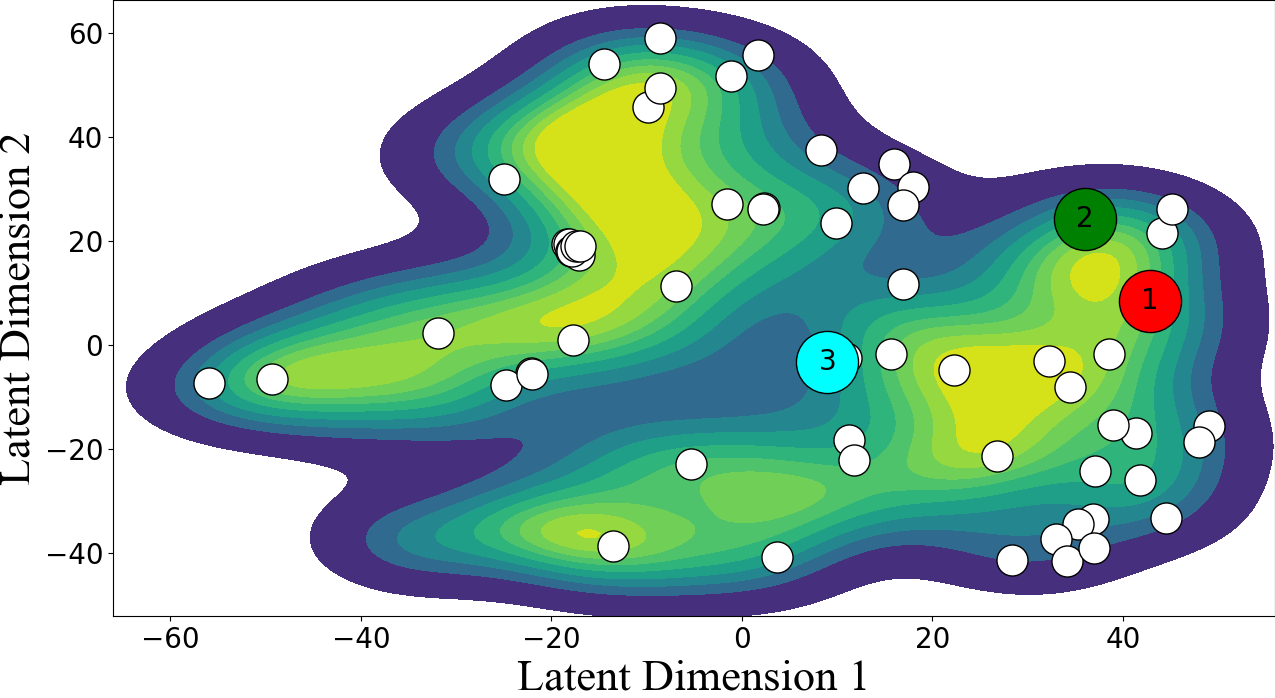
\includegraphics[width=\columnwidth]{chp_sogp/figures/TSNE_task4_kde_p30.png}
			\caption{Reservoir E.}
		\end{subfigure}
		\hspace{0.05\columnwidth} % Reduced space between columns
		\begin{subfigure}[t]{0.38\columnwidth}
			\centering
			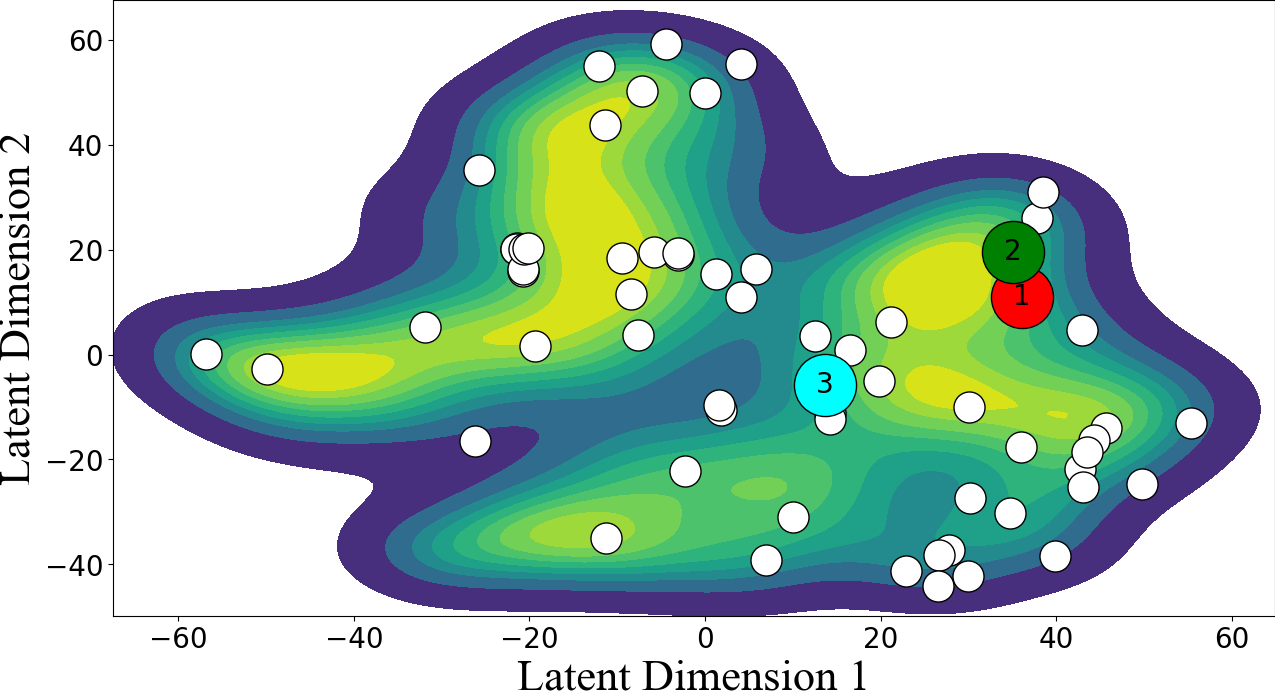
\includegraphics[width=\columnwidth]{chp_sogp/figures/TSNE_task8_kde_p30.png}
			\caption{Reservoir I.}
		\end{subfigure}
		
		\vspace{0.1cm} % Space between rows
		
		\begin{subfigure}[t]{0.38\columnwidth}
			\centering
			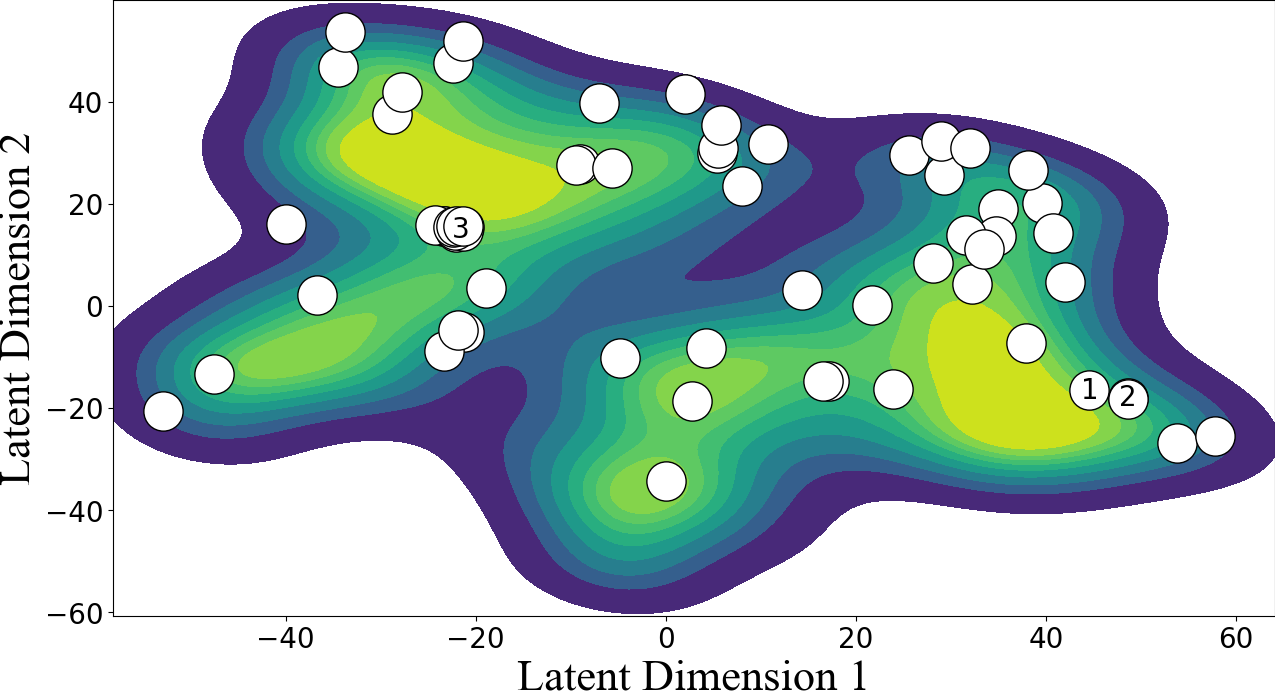
\includegraphics[width=\columnwidth]{chp_sogp/figures/TSNE_task11_kde_p30.png}
			\caption{Reservoir L.}
		\end{subfigure}
		\hspace{0.05\columnwidth} % Reduced space between columns
		\begin{subfigure}[t]{0.38\columnwidth}
			\centering
			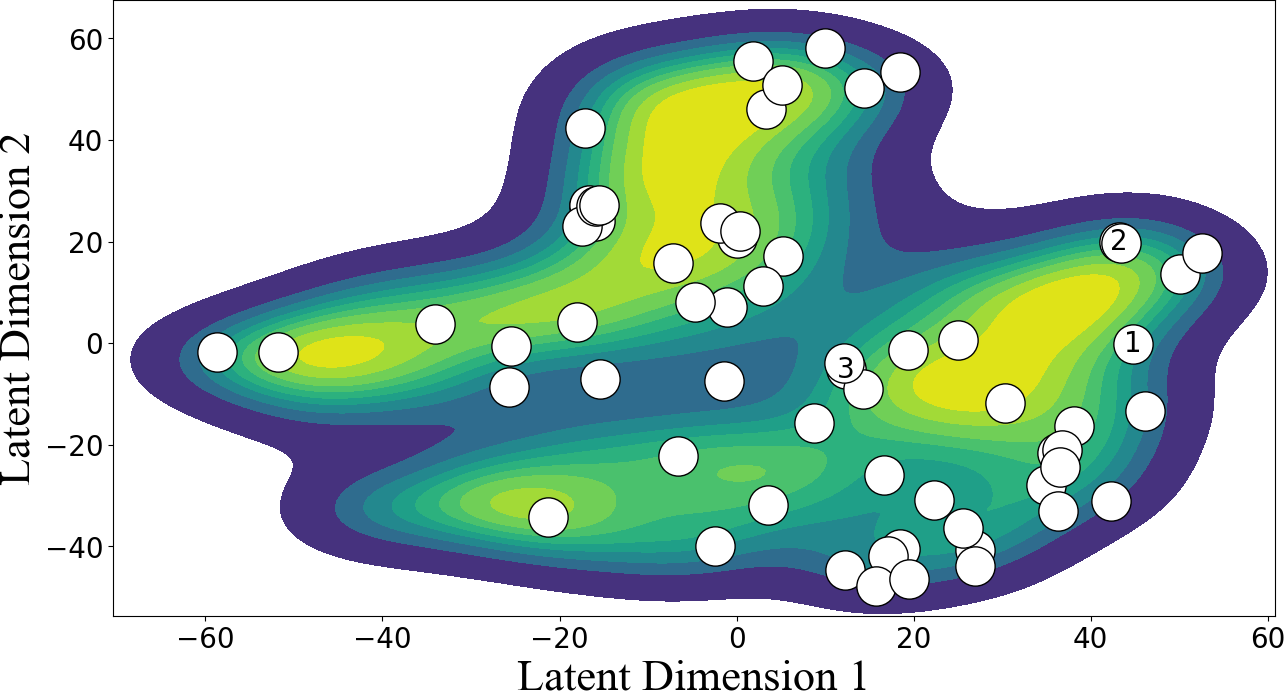
\includegraphics[width=\columnwidth]{chp_sogp/figures/TSNE_task20_kde_p30.png}
			\caption{Reservoir U.}
		\end{subfigure}
		
		\vspace{0.0cm} % Space between the figures and the caption
	\end{figure}
	t-SNE-based 2D mapping of the SVGP latent space and inducing points' locations for four target reservoirs. The shared inducing points allow for the capturing of task-wise, and global information about the streamflow dynamics.
\end{frame}


\subsubsection{Performance Analysis}


\begin{frame}{Models Forecasting}
	\begin{figure}[htbp]
		\centering
		\setlength\figurewidth{\columnwidth} 
		\setlength\figureheight{0.24\columnwidth}
		
		% This file was created with tikzplotlib v0.10.1.
\begin{tikzpicture}

\definecolor{darkgray176}{RGB}{176,176,176}
\definecolor{goldenrod1911910}{RGB}{191,191,0}
\definecolor{green01270}{RGB}{0,127,0}

\begin{axis}[
	width=\figurewidth,
	height=\figureheight,
	axis background/.style={fill=background_color},
	axis line style={white},
	tick align=inside,
	tick pos=left,
	x grid style={white},
	y grid style={white},
	xmajorgrids,
	ymajorgrids,
	ylabel={Contributions (kWh)},
	ylabel style={font=\tiny},
	xmin=100, xmax=250,
	xtick style={color=white},
	ymin=-1179761.11521924, ymax=11048199.3095146,
	ytick style={color=black},
	xtick style={color=black},
	ytick={-2000000,0,2000000,4000000,6000000,8000000,10000000,12000000},
	yticklabels={\ensuremath{-}0.2,0.0,0.2,0.4,0.6,0.8,1.0,1.2},
	tick label style={font=\tiny}  % For the tick labels
	% ylabel style={font=\tiny},
	]

\path [draw=blue, fill=blue, opacity=0.5]
(axis cs:0,3108233.88889613)
--(axis cs:0,-65315.7661637515)
--(axis cs:1,669228.387932176)
--(axis cs:2,1419260.840623)
--(axis cs:3,570172.276784107)
--(axis cs:4,696740.089543019)
--(axis cs:5,745623.738734278)
--(axis cs:6,923699.266685501)
--(axis cs:7,624021.308190048)
--(axis cs:8,1109759.03139669)
--(axis cs:9,1951556.74967448)
--(axis cs:10,1226283.29840689)
--(axis cs:11,825924.356937511)
--(axis cs:12,831458.852584676)
--(axis cs:13,1138171.45305888)
--(axis cs:14,3131044.80865211)
--(axis cs:15,2465943.35115869)
--(axis cs:16,637623.524270154)
--(axis cs:17,1550040.65483331)
--(axis cs:18,1725412.19366463)
--(axis cs:19,1202296.54926133)
--(axis cs:20,4168226.80093676)
--(axis cs:21,2248825.1965464)
--(axis cs:22,2624957.04407417)
--(axis cs:23,1794681.85002759)
--(axis cs:24,1637109.03927698)
--(axis cs:25,1429245.86115541)
--(axis cs:26,2457939.67555987)
--(axis cs:27,2006540.65218201)
--(axis cs:28,2094275.79391441)
--(axis cs:29,2044682.43815446)
--(axis cs:30,2070115.58808654)
--(axis cs:31,1600612.08536125)
--(axis cs:32,1505670.97578632)
--(axis cs:33,2021127.05340145)
--(axis cs:34,1781051.3712567)
--(axis cs:35,1801361.80250696)
--(axis cs:36,1845733.09235211)
--(axis cs:37,2771867.68531726)
--(axis cs:38,2897495.04765516)
--(axis cs:39,2399498.62002586)
--(axis cs:40,1633190.63728418)
--(axis cs:41,2201680.99572401)
--(axis cs:42,2737506.30038491)
--(axis cs:43,2738438.91186965)
--(axis cs:44,4074201.20888666)
--(axis cs:45,5097883.73970068)
--(axis cs:46,4530764.34910007)
--(axis cs:47,3903803.58717038)
--(axis cs:48,4778982.58123294)
--(axis cs:49,4469680.16168432)
--(axis cs:50,4725439.27191362)
--(axis cs:51,4127320.46922022)
--(axis cs:52,4677694.17742211)
--(axis cs:53,4881165.90202551)
--(axis cs:54,4201769.95097997)
--(axis cs:55,4220879.91874629)
--(axis cs:56,4665989.13275011)
--(axis cs:57,5099952.78509696)
--(axis cs:58,4075674.91148454)
--(axis cs:59,3693173.42993382)
--(axis cs:60,3299571.31989639)
--(axis cs:61,4105949.43749291)
--(axis cs:62,2634962.63551114)
--(axis cs:63,2294116.67951235)
--(axis cs:64,1837976.4821815)
--(axis cs:65,1756377.68842163)
--(axis cs:66,1778899.85716407)
--(axis cs:67,1259469.04821166)
--(axis cs:68,1170514.52913145)
--(axis cs:69,1176714.28654669)
--(axis cs:70,1119156.69199197)
--(axis cs:71,1232473.89471996)
--(axis cs:72,1301353.17992636)
--(axis cs:73,1121346.7627608)
--(axis cs:74,1176323.25802374)
--(axis cs:75,1137027.836719)
--(axis cs:76,1015210.842426)
--(axis cs:77,988017.070909713)
--(axis cs:78,881983.490356931)
--(axis cs:79,795861.805891391)
--(axis cs:80,577541.674495122)
--(axis cs:81,491620.422452393)
--(axis cs:82,649074.001789769)
--(axis cs:83,614319.919233096)
--(axis cs:84,446796.387611155)
--(axis cs:85,469760.398863785)
--(axis cs:86,370736.180430243)
--(axis cs:87,360472.459061581)
--(axis cs:88,404973.980320668)
--(axis cs:89,1079126.33722617)
--(axis cs:90,2278274.27220474)
--(axis cs:91,1280229.53109866)
--(axis cs:92,1095566.19047506)
--(axis cs:93,1345174.61054887)
--(axis cs:94,1110104.40772488)
--(axis cs:95,2088145.58067334)
--(axis cs:96,1518108.37555543)
--(axis cs:97,1465383.57719615)
--(axis cs:98,2570632.20629951)
--(axis cs:99,2612092.82410822)
--(axis cs:100,2243732.3432516)
--(axis cs:101,2557798.58285646)
--(axis cs:102,3378272.89569686)
--(axis cs:103,2749072.02697939)
--(axis cs:104,1921757.05223719)
--(axis cs:105,1930107.17634567)
--(axis cs:106,1627786.3605072)
--(axis cs:107,1887232.06468482)
--(axis cs:108,2194539.20364258)
--(axis cs:109,3978587.84741291)
--(axis cs:110,4150172.08623071)
--(axis cs:111,2833983.00021501)
--(axis cs:112,3586871.142694)
--(axis cs:113,3095169.20451087)
--(axis cs:114,3168859.50861122)
--(axis cs:115,3050589.94818455)
--(axis cs:116,2489256.23136287)
--(axis cs:117,2796172.92129639)
--(axis cs:118,4075356.89734583)
--(axis cs:119,3292960.73153601)
--(axis cs:120,3502094.39441298)
--(axis cs:121,2981762.32745178)
--(axis cs:122,3005960.99217388)
--(axis cs:123,2940799.90223084)
--(axis cs:124,3300245.80404193)
--(axis cs:125,3962420.4813777)
--(axis cs:126,3785354.84800194)
--(axis cs:127,4699808.04991838)
--(axis cs:128,3538091.51536115)
--(axis cs:129,2878034.566322)
--(axis cs:130,3952222.40198661)
--(axis cs:131,4130927.02883305)
--(axis cs:132,3142452.44821017)
--(axis cs:133,3121346.44807595)
--(axis cs:134,3157954.19034543)
--(axis cs:135,2778604.5932361)
--(axis cs:136,2353401.24601781)
--(axis cs:137,2095674.36616339)
--(axis cs:138,1519205.32581629)
--(axis cs:139,1752614.61315188)
--(axis cs:140,1447891.91078644)
--(axis cs:141,1617449.27798012)
--(axis cs:142,1676874.62604652)
--(axis cs:143,1559596.42653098)
--(axis cs:144,1193575.15833361)
--(axis cs:145,1558274.03339233)
--(axis cs:146,1503682.61037281)
--(axis cs:147,1436610.58200666)
--(axis cs:148,1399976.41525141)
--(axis cs:149,1328167.8430371)
--(axis cs:150,1458541.68965385)
--(axis cs:151,886615.565599867)
--(axis cs:152,1037365.48577945)
--(axis cs:153,806934.71954604)
--(axis cs:154,1219752.10455162)
--(axis cs:155,1193669.3874732)
--(axis cs:156,919103.15455863)
--(axis cs:157,953086.992339702)
--(axis cs:158,1166464.96973863)
--(axis cs:159,1068363.53556173)
--(axis cs:160,1872918.22142661)
--(axis cs:161,1467198.13951965)
--(axis cs:162,1084889.37541884)
--(axis cs:163,1352992.91694775)
--(axis cs:164,1031361.32942225)
--(axis cs:165,1560729.04313472)
--(axis cs:166,1891183.02891173)
--(axis cs:167,3912074.78803338)
--(axis cs:168,3601805.86694718)
--(axis cs:169,3448586.63396685)
--(axis cs:170,4112820.83618656)
--(axis cs:171,4062598.48636038)
--(axis cs:172,4121106.52639912)
--(axis cs:173,2464073.39101171)
--(axis cs:174,2559818.9853543)
--(axis cs:175,3107042.5814636)
--(axis cs:176,2934449.54489105)
--(axis cs:177,3345948.68097132)
--(axis cs:178,2852704.36895256)
--(axis cs:179,2320301.66282545)
--(axis cs:180,2766266.11282191)
--(axis cs:181,2879095.60692391)
--(axis cs:182,2242229.1853233)
--(axis cs:183,1944684.29483982)
--(axis cs:184,2349554.63456829)
--(axis cs:185,3453665.20597057)
--(axis cs:186,2151358.73816853)
--(axis cs:187,2550126.60287753)
--(axis cs:188,2848706.97007814)
--(axis cs:189,2249879.74472523)
--(axis cs:190,1699185.71525415)
--(axis cs:191,1636130.46397808)
--(axis cs:192,959371.115525304)
--(axis cs:193,1378339.70139651)
--(axis cs:194,589463.002962724)
--(axis cs:195,1274513.25474179)
--(axis cs:196,1492004.50155959)
--(axis cs:197,1943056.36784977)
--(axis cs:198,1965554.41003327)
--(axis cs:199,2355228.80420998)
--(axis cs:200,1609144.22575292)
--(axis cs:201,1228966.09030714)
--(axis cs:202,2077776.10440912)
--(axis cs:203,2652925.26726529)
--(axis cs:204,1758355.45664699)
--(axis cs:205,1923730.22576374)
--(axis cs:206,1681726.55587874)
--(axis cs:207,2083466.28595586)
--(axis cs:208,3216978.93479361)
--(axis cs:209,4292274.69459285)
--(axis cs:210,3966990.68192498)
--(axis cs:211,2349986.87907274)
--(axis cs:212,2604424.1430523)
--(axis cs:213,3067440.19714662)
--(axis cs:214,3405860.17700633)
--(axis cs:215,4943121.72895524)
--(axis cs:216,4202654.24241601)
--(axis cs:217,2949256.84274647)
--(axis cs:218,2449415.56619626)
--(axis cs:219,1920914.57828096)
--(axis cs:220,929330.648530921)
--(axis cs:221,2340800.05431662)
--(axis cs:222,1546705.20416566)
--(axis cs:223,1642608.64080335)
--(axis cs:224,883998.928757176)
--(axis cs:225,2168914.1378654)
--(axis cs:226,1769577.4552714)
--(axis cs:227,1771596.25594639)
--(axis cs:228,1640246.23195452)
--(axis cs:229,1363744.06910245)
--(axis cs:230,1482488.26551172)
--(axis cs:231,2279203.05850897)
--(axis cs:232,1439568.72487413)
--(axis cs:233,973083.286835435)
--(axis cs:234,687230.412678654)
--(axis cs:235,312253.526647817)
--(axis cs:236,258737.131321228)
--(axis cs:237,518507.503939466)
--(axis cs:238,507800.286963373)
--(axis cs:239,714547.873918125)
--(axis cs:240,745927.897424996)
--(axis cs:241,282367.369705169)
--(axis cs:242,1080877.05592759)
--(axis cs:243,1021986.95275863)
--(axis cs:244,1359172.38633743)
--(axis cs:245,560797.015431945)
--(axis cs:246,253398.578534735)
--(axis cs:247,122369.740913339)
--(axis cs:248,142119.621914188)
--(axis cs:249,1461008.62917028)
--(axis cs:250,1382852.34753051)
--(axis cs:251,1337661.27940971)
--(axis cs:252,2516166.08533359)
--(axis cs:253,2756116.04618681)
--(axis cs:254,1945868.95830688)
--(axis cs:255,742318.822901707)
--(axis cs:256,590845.449014683)
--(axis cs:257,732376.712000819)
--(axis cs:258,371823.473995499)
--(axis cs:259,498790.179361989)
--(axis cs:260,-70478.9566171567)
--(axis cs:261,-132251.655877984)
--(axis cs:262,-308222.28234103)
--(axis cs:263,-90728.4051710551)
--(axis cs:264,1527164.01834468)
--(axis cs:265,333488.503402017)
--(axis cs:266,-133047.526604814)
--(axis cs:267,-357513.241422475)
--(axis cs:268,-478743.410889146)
--(axis cs:269,-508653.362335969)
--(axis cs:270,-519950.869457445)
--(axis cs:271,307796.04517069)
--(axis cs:272,-452663.701540708)
--(axis cs:273,128543.491422936)
--(axis cs:274,533125.759543572)
--(axis cs:275,-78387.2607954545)
--(axis cs:276,148498.283902145)
--(axis cs:277,295904.219136156)
--(axis cs:278,400127.95458363)
--(axis cs:279,851454.551932115)
--(axis cs:280,903007.821231771)
--(axis cs:281,290378.566820613)
--(axis cs:282,336658.816592991)
--(axis cs:283,167112.737213447)
--(axis cs:284,-51517.6060490157)
--(axis cs:285,77759.8657282244)
--(axis cs:286,1733056.94577668)
--(axis cs:287,1684926.05293574)
--(axis cs:288,654751.076894854)
--(axis cs:289,818768.193903532)
--(axis cs:290,172607.136405745)
--(axis cs:291,28845.5665919657)
--(axis cs:292,349585.529706082)
--(axis cs:293,493734.408109412)
--(axis cs:294,125135.184603735)
--(axis cs:295,202809.208816265)
--(axis cs:296,-46130.7569099448)
--(axis cs:297,-280234.963308346)
--(axis cs:298,896913.59074457)
--(axis cs:299,629591.565716487)
--(axis cs:300,408540.131126394)
--(axis cs:301,-55601.2830621088)
--(axis cs:302,-50333.9842510642)
--(axis cs:303,243070.962650516)
--(axis cs:304,361420.576386839)
--(axis cs:305,71272.5634133297)
--(axis cs:306,-142429.213645665)
--(axis cs:307,-157692.033044641)
--(axis cs:308,-125493.026506122)
--(axis cs:309,-348581.296523267)
--(axis cs:310,-234627.839723981)
--(axis cs:311,-396407.873707958)
--(axis cs:312,-327417.366030162)
--(axis cs:313,-623944.732276791)
--(axis cs:314,-200804.454074635)
--(axis cs:315,636464.61417112)
--(axis cs:316,36218.3462727345)
--(axis cs:317,-374198.868093826)
--(axis cs:318,-390782.20310167)
--(axis cs:319,-429763.444203756)
--(axis cs:320,-275900.558233003)
--(axis cs:321,-326138.92104813)
--(axis cs:322,732590.18684618)
--(axis cs:323,298834.346026512)
--(axis cs:324,-381681.999621222)
--(axis cs:325,-368912.728350223)
--(axis cs:326,-122099.660133952)
--(axis cs:327,257816.579930977)
--(axis cs:328,523433.603494196)
--(axis cs:329,632449.257758414)
--(axis cs:330,1099057.07088521)
--(axis cs:331,1977155.4207391)
--(axis cs:332,1561912.86669768)
--(axis cs:333,2125052.90304491)
--(axis cs:334,1856749.33698707)
--(axis cs:335,1318188.93894391)
--(axis cs:336,1026072.58746103)
--(axis cs:337,1039450.28481819)
--(axis cs:338,1470833.30857286)
--(axis cs:339,1703199.11573354)
--(axis cs:340,1447347.68431838)
--(axis cs:341,920717.257977744)
--(axis cs:342,813751.199442925)
--(axis cs:343,2687428.09755101)
--(axis cs:344,1899966.312076)
--(axis cs:345,2434485.11867734)
--(axis cs:346,2250715.34150529)
--(axis cs:347,1829655.83957436)
--(axis cs:348,1705881.6420401)
--(axis cs:349,2405727.63936495)
--(axis cs:350,2384057.00460254)
--(axis cs:351,2229468.25155866)
--(axis cs:352,2380090.19902676)
--(axis cs:353,3325722.73365308)
--(axis cs:354,2009772.8213879)
--(axis cs:355,2830020.4771571)
--(axis cs:356,3017464.12040618)
--(axis cs:357,3274221.47463156)
--(axis cs:358,2472842.02740586)
--(axis cs:359,2234999.14826375)
--(axis cs:360,1722256.4353719)
--(axis cs:361,1781986.88568117)
--(axis cs:362,3829961.58953858)
--(axis cs:363,3009651.48713282)
--(axis cs:364,5795738.4692333)
--(axis cs:365,3780200.18679237)
--(axis cs:366,5042418.18644462)
--(axis cs:367,4948959.57713539)
--(axis cs:368,4815233.78375167)
--(axis cs:369,4213061.00629453)
--(axis cs:370,3311143.95803368)
--(axis cs:371,3260747.58641513)
--(axis cs:372,4909151.55351126)
--(axis cs:373,5040704.04753161)
--(axis cs:374,4715113.48711086)
--(axis cs:375,4750680.48472726)
--(axis cs:376,5177229.28752918)
--(axis cs:377,6516791.49810697)
--(axis cs:378,5980540.84752969)
--(axis cs:379,5569850.32825593)
--(axis cs:380,5416645.36536457)
--(axis cs:381,4213177.27781981)
--(axis cs:382,5196133.25142109)
--(axis cs:383,4951351.72584528)
--(axis cs:384,4172886.90216458)
--(axis cs:385,3448543.91424146)
--(axis cs:386,3559767.12159882)
--(axis cs:387,3505667.09691641)
--(axis cs:388,3183153.9154571)
--(axis cs:389,3256131.0265355)
--(axis cs:390,2570236.29118108)
--(axis cs:391,2449446.02716161)
--(axis cs:392,2537606.67571818)
--(axis cs:393,2509178.08363911)
--(axis cs:394,4122195.63175771)
--(axis cs:395,4711143.90833355)
--(axis cs:396,5368249.41594041)
--(axis cs:397,4438819.8038216)
--(axis cs:398,3967584.90908379)
--(axis cs:399,3437076.71622112)
--(axis cs:400,2926974.98982679)
--(axis cs:401,3165824.17357294)
--(axis cs:402,2989161.88934761)
--(axis cs:403,2986619.77462832)
--(axis cs:404,3420272.47505006)
--(axis cs:405,3749372.25404147)
--(axis cs:406,3381268.57272193)
--(axis cs:407,2651224.2879894)
--(axis cs:408,2468294.79174326)
--(axis cs:409,2642762.38903544)
--(axis cs:410,3083580.1571857)
--(axis cs:411,2606413.97699711)
--(axis cs:412,2955642.6049086)
--(axis cs:413,3029534.05817418)
--(axis cs:414,3487297.93748435)
--(axis cs:415,4266132.41132912)
--(axis cs:416,4384200.19923679)
--(axis cs:417,4442434.16310703)
--(axis cs:418,3659412.16149907)
--(axis cs:419,4703870.82200459)
--(axis cs:420,4987285.93613191)
--(axis cs:421,2927445.81278105)
--(axis cs:422,3813811.39533037)
--(axis cs:423,3794494.73031793)
--(axis cs:424,3990146.66303102)
--(axis cs:425,4687925.90056945)
--(axis cs:426,3762621.93509526)
--(axis cs:427,3809463.42506402)
--(axis cs:428,3716270.78686259)
--(axis cs:429,3008151.43058207)
--(axis cs:430,2584131.47633207)
--(axis cs:431,2530396.91095458)
--(axis cs:432,2106445.88414099)
--(axis cs:433,1750221.80753047)
--(axis cs:434,1594932.24504578)
--(axis cs:435,1663209.83870175)
--(axis cs:436,1866007.02872755)
--(axis cs:437,2043430.36021905)
--(axis cs:438,1958193.5383167)
--(axis cs:439,2848638.38132314)
--(axis cs:440,1795961.68967574)
--(axis cs:440,4807070.04903816)
--(axis cs:440,4807070.04903816)
--(axis cs:439,6204880.77503505)
--(axis cs:438,4957748.0989974)
--(axis cs:437,5075940.33153258)
--(axis cs:436,4885618.74925267)
--(axis cs:435,4666967.86680518)
--(axis cs:434,4598828.27542495)
--(axis cs:433,4750129.32445001)
--(axis cs:432,5115952.79512073)
--(axis cs:431,5548114.10654931)
--(axis cs:430,5609252.54625718)
--(axis cs:429,6025555.62004322)
--(axis cs:428,6864369.68406398)
--(axis cs:427,6863218.57187474)
--(axis cs:426,6825893.07416793)
--(axis cs:425,7934891.9646613)
--(axis cs:424,7075280.28526413)
--(axis cs:423,6855034.12973609)
--(axis cs:422,6889059.63420582)
--(axis cs:421,6051947.9802743)
--(axis cs:420,8304899.22438623)
--(axis cs:419,7888241.78635925)
--(axis cs:418,6728018.9297872)
--(axis cs:417,7613984.17529088)
--(axis cs:416,7460156.20853873)
--(axis cs:415,7348608.04927564)
--(axis cs:414,6536956.91196541)
--(axis cs:413,6075434.73289871)
--(axis cs:412,6060732.7681522)
--(axis cs:411,5626278.49879478)
--(axis cs:410,6098980.25676155)
--(axis cs:409,5725332.73917514)
--(axis cs:408,5469076.97637315)
--(axis cs:407,5653857.8931386)
--(axis cs:406,6411670.39050845)
--(axis cs:405,6866746.99243879)
--(axis cs:404,6527862.02952526)
--(axis cs:403,6095813.93712054)
--(axis cs:402,6060402.96437552)
--(axis cs:401,6241782.35929358)
--(axis cs:400,5955550.21852487)
--(axis cs:399,6471067.44229152)
--(axis cs:398,7029935.29228495)
--(axis cs:397,7557663.15604346)
--(axis cs:396,8781355.23563886)
--(axis cs:395,8101997.99049796)
--(axis cs:394,7293915.25017464)
--(axis cs:393,5544633.47562903)
--(axis cs:392,5561195.87835914)
--(axis cs:391,5444600.80069617)
--(axis cs:390,5606105.90930873)
--(axis cs:389,6272245.81457965)
--(axis cs:388,6211999.37372955)
--(axis cs:387,6629664.22525488)
--(axis cs:386,6611044.59159048)
--(axis cs:385,6512266.20770119)
--(axis cs:384,7324587.53507791)
--(axis cs:383,8098548.71612909)
--(axis cs:382,8322561.3684983)
--(axis cs:381,7304447.79773261)
--(axis cs:380,8832206.31330609)
--(axis cs:379,9133550.02902922)
--(axis cs:378,9365038.64169209)
--(axis cs:377,9869397.17952286)
--(axis cs:376,8619846.71136419)
--(axis cs:375,7827909.64469325)
--(axis cs:374,7802338.40325687)
--(axis cs:373,8128301.09682379)
--(axis cs:372,8115730.01840282)
--(axis cs:371,6304381.23379707)
--(axis cs:370,6320221.74239068)
--(axis cs:369,7259338.50871168)
--(axis cs:368,7872888.17969077)
--(axis cs:367,8084376.46181158)
--(axis cs:366,8594773.3850251)
--(axis cs:365,6814281.91325362)
--(axis cs:364,8982843.18230157)
--(axis cs:363,6123188.77062267)
--(axis cs:362,7172739.61147288)
--(axis cs:361,4844559.10361851)
--(axis cs:360,4966943.6270199)
--(axis cs:359,5329811.44877875)
--(axis cs:358,5731545.91672336)
--(axis cs:357,6904327.46795872)
--(axis cs:356,6186141.03257335)
--(axis cs:355,5928371.23676601)
--(axis cs:354,5159754.55532811)
--(axis cs:353,6715389.13417894)
--(axis cs:352,5544165.64681618)
--(axis cs:351,5354461.80373196)
--(axis cs:350,5687069.93308737)
--(axis cs:349,5757126.87661865)
--(axis cs:348,4918895.28141451)
--(axis cs:347,4865437.6706578)
--(axis cs:346,5294726.51111172)
--(axis cs:345,5450041.37170463)
--(axis cs:344,5002614.64497402)
--(axis cs:343,5782837.28841288)
--(axis cs:342,4031507.05212974)
--(axis cs:341,4040384.93018393)
--(axis cs:340,4469157.75185626)
--(axis cs:339,4774865.368758)
--(axis cs:338,4654263.34770798)
--(axis cs:337,4160871.88430159)
--(axis cs:336,4297236.2848371)
--(axis cs:335,4339443.84168207)
--(axis cs:334,4867581.08169081)
--(axis cs:333,5220530.95025984)
--(axis cs:332,4677293.76935791)
--(axis cs:331,5066563.63072748)
--(axis cs:330,4149367.52022549)
--(axis cs:329,3970904.02174818)
--(axis cs:328,4007287.10657077)
--(axis cs:327,3375643.4079107)
--(axis cs:326,2967123.06629014)
--(axis cs:325,2703175.24685551)
--(axis cs:324,2896768.28953469)
--(axis cs:323,3507097.03567422)
--(axis cs:322,4130960.2227102)
--(axis cs:321,2767454.91485611)
--(axis cs:320,2763777.86349953)
--(axis cs:319,2586465.22699695)
--(axis cs:318,2646161.97016497)
--(axis cs:317,2673834.05736283)
--(axis cs:316,3213405.92578114)
--(axis cs:315,4766148.95976482)
--(axis cs:314,3557665.08020745)
--(axis cs:313,2670578.39442322)
--(axis cs:312,2679261.54995116)
--(axis cs:311,2643041.98966305)
--(axis cs:310,2767602.28516578)
--(axis cs:309,2641094.74577625)
--(axis cs:308,2874677.29232268)
--(axis cs:307,2948128.51351298)
--(axis cs:306,2881597.323139)
--(axis cs:305,3079838.69077048)
--(axis cs:304,3469928.89622474)
--(axis cs:303,3436295.11164106)
--(axis cs:302,3003234.33482164)
--(axis cs:301,3020773.48010767)
--(axis cs:300,3562783.96680598)
--(axis cs:299,3764655.33194601)
--(axis cs:298,4095594.47215417)
--(axis cs:297,2885300.09605325)
--(axis cs:296,2950059.22674525)
--(axis cs:295,3199141.49245568)
--(axis cs:294,3186424.76541765)
--(axis cs:293,3687100.60354983)
--(axis cs:292,3523803.61342062)
--(axis cs:291,3130249.10924002)
--(axis cs:290,3183201.16049211)
--(axis cs:289,4052458.1173081)
--(axis cs:288,3673817.63335514)
--(axis cs:287,4751155.28791322)
--(axis cs:286,4995923.46695312)
--(axis cs:285,3289386.4693148)
--(axis cs:284,3540937.04743021)
--(axis cs:283,3332864.73509378)
--(axis cs:282,3483961.48380458)
--(axis cs:281,3452867.66352428)
--(axis cs:280,4162822.81598416)
--(axis cs:279,4346287.76679997)
--(axis cs:278,3792813.90870439)
--(axis cs:277,3416376.92174048)
--(axis cs:276,3313608.3558041)
--(axis cs:275,3183100.83389819)
--(axis cs:274,3690182.05767661)
--(axis cs:273,3338166.5265189)
--(axis cs:272,2770466.96933592)
--(axis cs:271,3856131.01505078)
--(axis cs:270,2518970.68376983)
--(axis cs:269,2505640.88130832)
--(axis cs:268,2523830.13498204)
--(axis cs:267,2654871.35167218)
--(axis cs:266,2890591.11073807)
--(axis cs:265,3371969.48930829)
--(axis cs:264,4728326.42695912)
--(axis cs:263,2958945.23757947)
--(axis cs:262,2721734.08114153)
--(axis cs:261,2970733.116338)
--(axis cs:260,3681327.74232798)
--(axis cs:259,3581875.15127612)
--(axis cs:258,3413480.42590851)
--(axis cs:257,4004949.04286148)
--(axis cs:256,3684116.25028369)
--(axis cs:255,3928106.80701977)
--(axis cs:254,5283099.03776747)
--(axis cs:253,6164976.63192583)
--(axis cs:252,5912083.13317729)
--(axis cs:251,4693491.2223883)
--(axis cs:250,4522864.1731714)
--(axis cs:249,4699098.41396389)
--(axis cs:248,4024862.57617218)
--(axis cs:247,3774438.47955876)
--(axis cs:246,3520600.11898392)
--(axis cs:245,3609907.85039578)
--(axis cs:244,4458396.7613032)
--(axis cs:243,4285075.16681006)
--(axis cs:242,4435587.53032616)
--(axis cs:241,4169271.56746644)
--(axis cs:240,4050170.15535312)
--(axis cs:239,4126532.67484336)
--(axis cs:238,3913082.45191088)
--(axis cs:237,3527299.19287086)
--(axis cs:236,3259985.55494823)
--(axis cs:235,3313340.88938811)
--(axis cs:234,3682568.77676111)
--(axis cs:233,3967312.0694993)
--(axis cs:232,4738263.60693925)
--(axis cs:231,5327430.69082688)
--(axis cs:230,4531303.84307841)
--(axis cs:229,4476618.52591858)
--(axis cs:228,4712252.81320333)
--(axis cs:227,4863364.35814834)
--(axis cs:226,5015722.20773212)
--(axis cs:225,5230908.55970961)
--(axis cs:224,4874548.13373698)
--(axis cs:223,4804045.49713513)
--(axis cs:222,5001472.23697788)
--(axis cs:221,6416788.24781353)
--(axis cs:220,5320283.54887012)
--(axis cs:219,5627167.88240771)
--(axis cs:218,5791028.06320234)
--(axis cs:217,6155701.69715696)
--(axis cs:216,7466730.24182845)
--(axis cs:215,8694820.81548817)
--(axis cs:214,7107388.30994782)
--(axis cs:213,6926973.5845458)
--(axis cs:212,6585551.18300911)
--(axis cs:211,6241575.99783204)
--(axis cs:210,7264439.26772406)
--(axis cs:209,8078300.03185855)
--(axis cs:208,6893615.61369908)
--(axis cs:207,5292530.02147734)
--(axis cs:206,4903457.60554821)
--(axis cs:205,5228693.14396536)
--(axis cs:204,4930944.53658612)
--(axis cs:203,5996474.11521639)
--(axis cs:202,5762234.01844132)
--(axis cs:201,5486720.45234299)
--(axis cs:200,5539446.25811784)
--(axis cs:199,5770999.43995243)
--(axis cs:198,5210269.3695721)
--(axis cs:197,5347090.05588129)
--(axis cs:196,4736634.34703081)
--(axis cs:195,5003222.39310064)
--(axis cs:194,5082603.39026278)
--(axis cs:193,4661228.90406454)
--(axis cs:192,4308129.41336433)
--(axis cs:191,4898477.10784021)
--(axis cs:190,4712953.66993086)
--(axis cs:189,5314137.04523347)
--(axis cs:188,6094350.20248486)
--(axis cs:187,6759435.00724094)
--(axis cs:186,6158887.83082933)
--(axis cs:185,7116982.50475671)
--(axis cs:184,5898735.50915572)
--(axis cs:183,4988910.08891225)
--(axis cs:182,5422663.66109802)
--(axis cs:181,5954585.69938948)
--(axis cs:180,5956002.77071667)
--(axis cs:179,5962389.59441249)
--(axis cs:178,6103312.78259184)
--(axis cs:177,6667632.69055711)
--(axis cs:176,6201627.59579753)
--(axis cs:175,6491880.98859695)
--(axis cs:174,6073223.07589612)
--(axis cs:173,6309501.70867467)
--(axis cs:172,7820459.77540613)
--(axis cs:171,7494776.42887573)
--(axis cs:170,7271516.2758603)
--(axis cs:169,7183301.79305577)
--(axis cs:168,6911066.28739653)
--(axis cs:167,7025495.09340933)
--(axis cs:166,4989607.85077415)
--(axis cs:165,4567621.87710067)
--(axis cs:164,4012925.87741481)
--(axis cs:163,4360841.92630783)
--(axis cs:162,4385656.08159368)
--(axis cs:161,4454345.29815006)
--(axis cs:160,4882123.34161152)
--(axis cs:159,4057488.43015016)
--(axis cs:158,4203612.16929237)
--(axis cs:157,4075294.96699252)
--(axis cs:156,4264940.72818211)
--(axis cs:155,4229981.78274923)
--(axis cs:154,4367300.51117429)
--(axis cs:153,3902328.43340951)
--(axis cs:152,4050593.18065119)
--(axis cs:151,4460182.09293544)
--(axis cs:150,4500322.19546449)
--(axis cs:149,4356206.03282561)
--(axis cs:148,4789374.16316858)
--(axis cs:147,4457501.85901958)
--(axis cs:146,4592592.99682278)
--(axis cs:145,5067183.65699006)
--(axis cs:144,4525368.40207022)
--(axis cs:143,4615761.88507469)
--(axis cs:142,4779274.65596888)
--(axis cs:141,4686914.06177615)
--(axis cs:140,4523770.81764361)
--(axis cs:139,4881536.79729698)
--(axis cs:138,4791048.37815099)
--(axis cs:137,5199364.15857207)
--(axis cs:136,5416851.00048408)
--(axis cs:135,5991387.8489742)
--(axis cs:134,6432465.48276842)
--(axis cs:133,6309005.39528598)
--(axis cs:132,6819117.97354139)
--(axis cs:131,7388617.39497506)
--(axis cs:130,7347457.93193218)
--(axis cs:129,6224505.3496955)
--(axis cs:128,7060912.7343658)
--(axis cs:127,8150039.73220625)
--(axis cs:126,7557339.80020205)
--(axis cs:125,7313946.46770458)
--(axis cs:124,6562748.09740312)
--(axis cs:123,6596793.99491248)
--(axis cs:122,6122550.88819546)
--(axis cs:121,6355906.19725059)
--(axis cs:120,6911449.07859989)
--(axis cs:119,6379217.01684615)
--(axis cs:118,7169538.31281079)
--(axis cs:117,5834066.97572756)
--(axis cs:116,5966821.37859598)
--(axis cs:115,6123107.83496624)
--(axis cs:114,6243166.82306888)
--(axis cs:113,6412026.26161044)
--(axis cs:112,6770101.37309254)
--(axis cs:111,6362057.72808407)
--(axis cs:110,7414501.47187664)
--(axis cs:109,7142111.45129581)
--(axis cs:108,5231524.2790176)
--(axis cs:107,5108827.70600897)
--(axis cs:106,4940403.96028305)
--(axis cs:105,5046053.97808166)
--(axis cs:104,4921312.27945325)
--(axis cs:103,5773434.97199937)
--(axis cs:102,6507288.05511831)
--(axis cs:101,5588958.57807641)
--(axis cs:100,5304343.71586263)
--(axis cs:99,5634880.50748604)
--(axis cs:98,5594623.1340976)
--(axis cs:97,4454762.5148772)
--(axis cs:96,4513528.79549076)
--(axis cs:95,5141129.40776834)
--(axis cs:94,4109379.55627835)
--(axis cs:93,4339908.38997234)
--(axis cs:92,4098345.42503636)
--(axis cs:91,4276665.83775686)
--(axis cs:90,5323238.47475001)
--(axis cs:89,4096123.1941758)
--(axis cs:88,3388112.66109759)
--(axis cs:87,3339687.24079027)
--(axis cs:86,3362887.82601799)
--(axis cs:85,3581180.05276586)
--(axis cs:84,3441430.07151588)
--(axis cs:83,3593630.78761244)
--(axis cs:82,3644375.22777)
--(axis cs:81,3477107.88149855)
--(axis cs:80,3558900.74126377)
--(axis cs:79,3780846.50080497)
--(axis cs:78,3872513.19478714)
--(axis cs:77,3975640.45461195)
--(axis cs:76,4000073.48678522)
--(axis cs:75,4134468.96290668)
--(axis cs:74,4191387.07135822)
--(axis cs:73,4115075.68148878)
--(axis cs:72,4355323.35443294)
--(axis cs:71,4212780.01447395)
--(axis cs:70,4125039.93224711)
--(axis cs:69,4168473.85541341)
--(axis cs:68,4157207.47255826)
--(axis cs:67,4254115.84343482)
--(axis cs:66,4776608.45285336)
--(axis cs:65,4753389.39389148)
--(axis cs:64,4844886.05428035)
--(axis cs:63,5311411.06312842)
--(axis cs:62,5640468.91667264)
--(axis cs:61,7212391.90484769)
--(axis cs:60,6779155.11349918)
--(axis cs:59,6838577.67513793)
--(axis cs:58,7108805.37497294)
--(axis cs:57,8211238.93188273)
--(axis cs:56,7904453.08532865)
--(axis cs:55,7376509.87790499)
--(axis cs:54,7433180.59382883)
--(axis cs:53,8045551.43943408)
--(axis cs:52,7939369.10081075)
--(axis cs:51,7249296.13888991)
--(axis cs:50,7814330.46680189)
--(axis cs:49,7541788.60097599)
--(axis cs:48,7884925.78239554)
--(axis cs:47,6953047.93040545)
--(axis cs:46,7643721.74315804)
--(axis cs:45,8194538.10170071)
--(axis cs:44,7839379.91562723)
--(axis cs:43,6014420.91083554)
--(axis cs:42,5837567.48959546)
--(axis cs:41,5199441.99277919)
--(axis cs:40,4832482.79967473)
--(axis cs:39,5407410.5943689)
--(axis cs:38,5917799.59142355)
--(axis cs:37,5793349.69231323)
--(axis cs:36,4870487.27352628)
--(axis cs:35,4788569.95025397)
--(axis cs:34,4769497.97599156)
--(axis cs:33,5089569.82502238)
--(axis cs:32,4489922.44483318)
--(axis cs:31,4588707.38597667)
--(axis cs:30,5072130.11803369)
--(axis cs:29,5069424.78095438)
--(axis cs:28,5108401.02967648)
--(axis cs:27,5043727.62120074)
--(axis cs:26,5485911.99933344)
--(axis cs:25,4447845.49457724)
--(axis cs:24,4661569.10934291)
--(axis cs:23,4802455.07305418)
--(axis cs:22,5663617.8797525)
--(axis cs:21,5559457.43073985)
--(axis cs:20,7430015.70178711)
--(axis cs:19,4356971.07487856)
--(axis cs:18,4942348.12612545)
--(axis cs:17,4823473.21491361)
--(axis cs:16,5139378.03087491)
--(axis cs:15,5526556.43960021)
--(axis cs:14,6240472.48545879)
--(axis cs:13,4209308.0333661)
--(axis cs:12,3878000.58481799)
--(axis cs:11,3828491.33237935)
--(axis cs:10,4344809.45901802)
--(axis cs:9,5154492.19960987)
--(axis cs:8,4566418.29230597)
--(axis cs:7,4123906.56319744)
--(axis cs:6,4492690.90324228)
--(axis cs:5,4152368.33091657)
--(axis cs:4,4574404.72052272)
--(axis cs:3,3988789.67934708)
--(axis cs:2,4933353.84536417)
--(axis cs:1,4547977.92387378)
--(axis cs:0,3108233.88889613)
--cycle;

\path [draw=goldenrod1911910, fill=goldenrod1911910, opacity=0.5]
(axis cs:0,3200482.68971541)
--(axis cs:0,400593.213721099)
--(axis cs:1,922054.475448187)
--(axis cs:2,1783310.66399095)
--(axis cs:3,724029.858004906)
--(axis cs:4,881457.012457312)
--(axis cs:5,1155509.4218418)
--(axis cs:6,1422091.018899)
--(axis cs:7,1156205.58447469)
--(axis cs:8,1821835.67035793)
--(axis cs:9,2214860.40090517)
--(axis cs:10,1578835.87770593)
--(axis cs:11,1008573.83065008)
--(axis cs:12,1019380.60181513)
--(axis cs:13,1475467.80173748)
--(axis cs:14,3330509.58944005)
--(axis cs:15,2608825.07882214)
--(axis cs:16,2145454.30685822)
--(axis cs:17,1881341.02808239)
--(axis cs:18,2037072.95190258)
--(axis cs:19,1658567.12263739)
--(axis cs:20,4369008.91017082)
--(axis cs:21,2727889.75262147)
--(axis cs:22,2658632.82687842)
--(axis cs:23,1874794.21846243)
--(axis cs:24,1764787.77517605)
--(axis cs:25,1538113.24295467)
--(axis cs:26,2461251.21344626)
--(axis cs:27,1999981.57069115)
--(axis cs:28,2102016.86950225)
--(axis cs:29,2143273.03672141)
--(axis cs:30,2064619.69861195)
--(axis cs:31,1661544.82460462)
--(axis cs:32,1563892.87847036)
--(axis cs:33,2041480.54083205)
--(axis cs:34,1771388.7748551)
--(axis cs:35,1798081.36006882)
--(axis cs:36,1872100.99880894)
--(axis cs:37,2876676.94180933)
--(axis cs:38,2896256.4192961)
--(axis cs:39,2397092.08034458)
--(axis cs:40,1983815.40009012)
--(axis cs:41,2225980.32452435)
--(axis cs:42,2823244.27518467)
--(axis cs:43,3026318.75607584)
--(axis cs:44,5906040.27541999)
--(axis cs:45,5269846.13774991)
--(axis cs:46,4674333.45951414)
--(axis cs:47,4061782.6732726)
--(axis cs:48,5252975.76082645)
--(axis cs:49,4854452.9656079)
--(axis cs:50,5155821.86442435)
--(axis cs:51,4408107.92062101)
--(axis cs:52,5666651.60371894)
--(axis cs:53,5978757.31500816)
--(axis cs:54,5011623.09138473)
--(axis cs:55,4828842.38393287)
--(axis cs:56,5792238.03213389)
--(axis cs:57,5030512.71287101)
--(axis cs:58,3900763.61850027)
--(axis cs:59,3414843.94749268)
--(axis cs:60,3882182.60431962)
--(axis cs:61,4134484.18190493)
--(axis cs:62,2628469.29218526)
--(axis cs:63,2301120.57573437)
--(axis cs:64,1940214.73262366)
--(axis cs:65,1799466.93319913)
--(axis cs:66,1846502.49832779)
--(axis cs:67,1347206.28118601)
--(axis cs:68,1312927.98834491)
--(axis cs:69,1337523.75714735)
--(axis cs:70,1207276.5302437)
--(axis cs:71,1344969.4115158)
--(axis cs:72,1464563.14719502)
--(axis cs:73,1233174.89450432)
--(axis cs:74,1258102.90770569)
--(axis cs:75,1231983.04848435)
--(axis cs:76,1149041.35675701)
--(axis cs:77,1153843.29397661)
--(axis cs:78,1048236.41690743)
--(axis cs:79,969557.011735855)
--(axis cs:80,765031.711729812)
--(axis cs:81,647082.038213574)
--(axis cs:82,708050.590855822)
--(axis cs:83,719911.713429387)
--(axis cs:84,600411.864095268)
--(axis cs:85,581661.153020021)
--(axis cs:86,474412.785080879)
--(axis cs:87,527044.998460854)
--(axis cs:88,530852.812010713)
--(axis cs:89,1068038.54799497)
--(axis cs:90,2271644.81795421)
--(axis cs:91,1362702.44550038)
--(axis cs:92,1177283.04958917)
--(axis cs:93,1415438.36048357)
--(axis cs:94,1212873.56742784)
--(axis cs:95,2184012.61382728)
--(axis cs:96,1681038.45952261)
--(axis cs:97,1591843.84765469)
--(axis cs:98,2694612.39827764)
--(axis cs:99,2856222.58609156)
--(axis cs:100,2543599.04272396)
--(axis cs:101,2737044.05270009)
--(axis cs:102,3922558.85949709)
--(axis cs:103,2846871.80138486)
--(axis cs:104,2087975.00798083)
--(axis cs:105,2074100.49202866)
--(axis cs:106,1675532.98836337)
--(axis cs:107,1843014.09548152)
--(axis cs:108,2199624.60862119)
--(axis cs:109,4381251.86830154)
--(axis cs:110,4947697.78655264)
--(axis cs:111,4374113.11210862)
--(axis cs:112,4108917.68567526)
--(axis cs:113,3735942.23032344)
--(axis cs:114,3314006.08226851)
--(axis cs:115,3123349.90711376)
--(axis cs:116,2912326.80853454)
--(axis cs:117,2837060.18903574)
--(axis cs:118,4128762.42497071)
--(axis cs:119,3347937.33387675)
--(axis cs:120,3944888.72652037)
--(axis cs:121,3458433.93601942)
--(axis cs:122,3227840.70326892)
--(axis cs:123,4704840.16997533)
--(axis cs:124,3575925.86019908)
--(axis cs:125,3921211.67215774)
--(axis cs:126,4552772.93729974)
--(axis cs:127,4929576.23968759)
--(axis cs:128,3976271.14514871)
--(axis cs:129,3285683.72950626)
--(axis cs:130,4157338.46007302)
--(axis cs:131,4148590.00227747)
--(axis cs:132,3578143.6036107)
--(axis cs:133,3251672.92923823)
--(axis cs:134,3097363.29414066)
--(axis cs:135,3012214.22124796)
--(axis cs:136,2486579.99299022)
--(axis cs:137,2027833.84324337)
--(axis cs:138,1826120.00776184)
--(axis cs:139,1918242.33169307)
--(axis cs:140,1569447.98940317)
--(axis cs:141,1782860.34988622)
--(axis cs:142,1833116.70491309)
--(axis cs:143,1662314.83843847)
--(axis cs:144,1348567.95344934)
--(axis cs:145,1813045.47379266)
--(axis cs:146,1509690.99152576)
--(axis cs:147,1508728.8790474)
--(axis cs:148,1707967.84768732)
--(axis cs:149,1401667.96683981)
--(axis cs:150,1472137.406195)
--(axis cs:151,1366523.16494052)
--(axis cs:152,1208390.26490349)
--(axis cs:153,1085409.66978546)
--(axis cs:154,1283529.90278781)
--(axis cs:155,1187593.57887327)
--(axis cs:156,1180307.21672216)
--(axis cs:157,1101477.13097143)
--(axis cs:158,1382170.94207437)
--(axis cs:159,1155127.26639996)
--(axis cs:160,1855321.46962736)
--(axis cs:161,1477700.83921945)
--(axis cs:162,1341095.60114523)
--(axis cs:163,1299398.49859266)
--(axis cs:164,1106812.27251932)
--(axis cs:165,1549723.75881897)
--(axis cs:166,2037201.81123816)
--(axis cs:167,3572100.00921375)
--(axis cs:168,3735525.01728366)
--(axis cs:169,4702595.26985066)
--(axis cs:170,4061399.00779002)
--(axis cs:171,4247754.87337404)
--(axis cs:172,4256555.35512993)
--(axis cs:173,3094065.86560536)
--(axis cs:174,2916549.32739979)
--(axis cs:175,3217328.35533129)
--(axis cs:176,3008891.42656697)
--(axis cs:177,3315075.79936669)
--(axis cs:178,2760540.76216605)
--(axis cs:179,2495643.26885409)
--(axis cs:180,2961489.31325874)
--(axis cs:181,2851209.23848564)
--(axis cs:182,2357418.20070272)
--(axis cs:183,2076880.46067526)
--(axis cs:184,2810802.44619368)
--(axis cs:185,3891308.26916616)
--(axis cs:186,3369976.5909374)
--(axis cs:187,3317492.60230941)
--(axis cs:188,2890818.40348668)
--(axis cs:189,2278127.17338634)
--(axis cs:190,1834932.59583648)
--(axis cs:191,1921534.80524702)
--(axis cs:192,1524147.56540294)
--(axis cs:193,1754069.12359724)
--(axis cs:194,1244701.13889856)
--(axis cs:195,1756917.02785478)
--(axis cs:196,1865775.46120768)
--(axis cs:197,2338473.62642687)
--(axis cs:198,2214689.80412666)
--(axis cs:199,2642452.08815224)
--(axis cs:200,2550061.76044432)
--(axis cs:201,2881565.03460031)
--(axis cs:202,2143566.4808306)
--(axis cs:203,2855551.7392984)
--(axis cs:204,2102993.36392006)
--(axis cs:205,2023068.97296999)
--(axis cs:206,1862713.68900796)
--(axis cs:207,2243697.30916355)
--(axis cs:208,3851922.70432942)
--(axis cs:209,4915343.36325648)
--(axis cs:210,3956379.88085468)
--(axis cs:211,3864849.98452499)
--(axis cs:212,3630670.84094453)
--(axis cs:213,3503200.31596601)
--(axis cs:214,4114595.2477513)
--(axis cs:215,5207673.77219698)
--(axis cs:216,3999802.50124941)
--(axis cs:217,3061814.61214317)
--(axis cs:218,2488942.39163527)
--(axis cs:219,2592367.75831763)
--(axis cs:220,2504107.3314743)
--(axis cs:221,2600615.49564017)
--(axis cs:222,1986684.25183854)
--(axis cs:223,1892588.63206697)
--(axis cs:224,1929306.81845312)
--(axis cs:225,2194608.15989268)
--(axis cs:226,1887523.71555924)
--(axis cs:227,1914581.68290236)
--(axis cs:228,1703998.96805561)
--(axis cs:229,1486811.04237632)
--(axis cs:230,1526656.4292517)
--(axis cs:231,2244938.53014117)
--(axis cs:232,1333576.80852007)
--(axis cs:233,1096688.87481649)
--(axis cs:234,869349.620487842)
--(axis cs:235,516732.515815411)
--(axis cs:236,473702.473774688)
--(axis cs:237,718817.21912019)
--(axis cs:238,768829.451006359)
--(axis cs:239,766885.034526033)
--(axis cs:240,971638.495340992)
--(axis cs:241,741559.691733828)
--(axis cs:242,1179455.46008468)
--(axis cs:243,824083.033089558)
--(axis cs:244,1329208.13162557)
--(axis cs:245,726024.351176991)
--(axis cs:246,573905.456616644)
--(axis cs:247,482826.974187297)
--(axis cs:248,340029.34948934)
--(axis cs:249,1187300.72158794)
--(axis cs:250,1233665.82443299)
--(axis cs:251,842516.366343276)
--(axis cs:252,2929871.92163101)
--(axis cs:253,3417666.95793904)
--(axis cs:254,2301325.17221207)
--(axis cs:255,1148548.90413091)
--(axis cs:256,969352.657916971)
--(axis cs:257,1188921.18335333)
--(axis cs:258,596517.458913924)
--(axis cs:259,692321.716528729)
--(axis cs:260,391120.392777027)
--(axis cs:261,141847.044041976)
--(axis cs:262,-93778.0577271823)
--(axis cs:263,36931.5015527057)
--(axis cs:264,1496097.14367205)
--(axis cs:265,497540.713333014)
--(axis cs:266,83541.4706110912)
--(axis cs:267,-138368.256012584)
--(axis cs:268,-210516.049259564)
--(axis cs:269,-242296.002362918)
--(axis cs:270,-290410.384659413)
--(axis cs:271,411203.854063173)
--(axis cs:272,-290834.41939262)
--(axis cs:273,486745.422278199)
--(axis cs:274,707352.949226174)
--(axis cs:275,534812.672279151)
--(axis cs:276,452411.463629316)
--(axis cs:277,681319.380052655)
--(axis cs:278,603728.19400867)
--(axis cs:279,534431.913215469)
--(axis cs:280,1219686.9679987)
--(axis cs:281,749113.293720462)
--(axis cs:282,704306.278130895)
--(axis cs:283,369211.292435289)
--(axis cs:284,446900.97431517)
--(axis cs:285,598302.338665566)
--(axis cs:286,1911491.5452687)
--(axis cs:287,1812239.46496958)
--(axis cs:288,895178.447150833)
--(axis cs:289,1054002.99583312)
--(axis cs:290,451644.093117767)
--(axis cs:291,587422.595120622)
--(axis cs:292,733359.975913584)
--(axis cs:293,558923.174802154)
--(axis cs:294,262580.298501766)
--(axis cs:295,386066.791317214)
--(axis cs:296,213457.994455928)
--(axis cs:297,209601.112155967)
--(axis cs:298,1028568.68889991)
--(axis cs:299,872070.673524734)
--(axis cs:300,684294.76799828)
--(axis cs:301,141973.617540571)
--(axis cs:302,226840.598722606)
--(axis cs:303,296436.990999354)
--(axis cs:304,552056.694166492)
--(axis cs:305,226810.466906088)
--(axis cs:306,165344.687575334)
--(axis cs:307,37834.1493415488)
--(axis cs:308,26010.7050138884)
--(axis cs:309,-123096.543313616)
--(axis cs:310,-72910.834980655)
--(axis cs:311,-243541.993728044)
--(axis cs:312,-159052.20316986)
--(axis cs:313,-111097.70483316)
--(axis cs:314,17422.3270204822)
--(axis cs:315,692967.151589719)
--(axis cs:316,272936.934327276)
--(axis cs:317,-167936.591880004)
--(axis cs:318,-251656.010520827)
--(axis cs:319,-251963.863643992)
--(axis cs:320,-151984.486492381)
--(axis cs:321,-114129.687958614)
--(axis cs:322,1072916.13236232)
--(axis cs:323,426089.983297765)
--(axis cs:324,159771.578625279)
--(axis cs:325,-26552.3764635976)
--(axis cs:326,124748.577129562)
--(axis cs:327,551052.552634699)
--(axis cs:328,740063.520379904)
--(axis cs:329,856672.684063183)
--(axis cs:330,1147125.25470274)
--(axis cs:331,2020755.27893341)
--(axis cs:332,1670997.3366997)
--(axis cs:333,2168809.97885989)
--(axis cs:334,1912603.20706038)
--(axis cs:335,1427059.2979767)
--(axis cs:336,1211731.06692569)
--(axis cs:337,1110111.28501001)
--(axis cs:338,1799137.56253503)
--(axis cs:339,1827799.53154272)
--(axis cs:340,1528620.11648272)
--(axis cs:341,1284587.17901294)
--(axis cs:342,1189417.53413055)
--(axis cs:343,2699830.07714076)
--(axis cs:344,2154723.80807708)
--(axis cs:345,2458254.22201508)
--(axis cs:346,2344352.26200745)
--(axis cs:347,1994538.50134908)
--(axis cs:348,1988602.92018705)
--(axis cs:349,2772545.65131986)
--(axis cs:350,2740045.86266744)
--(axis cs:351,2396912.34752592)
--(axis cs:352,2524125.96482483)
--(axis cs:353,3416385.61848837)
--(axis cs:354,2217713.07508349)
--(axis cs:355,2863850.67679323)
--(axis cs:356,3185675.51550628)
--(axis cs:357,3965888.69360284)
--(axis cs:358,3055480.86332814)
--(axis cs:359,2467116.2445345)
--(axis cs:360,2073028.14376546)
--(axis cs:361,1967496.47174063)
--(axis cs:362,4149214.16662886)
--(axis cs:363,3130269.29145103)
--(axis cs:364,5844328.78165315)
--(axis cs:365,3751177.22083661)
--(axis cs:366,5905802.99660668)
--(axis cs:367,4832766.78398308)
--(axis cs:368,4628261.10064507)
--(axis cs:369,4198606.23934772)
--(axis cs:370,3331411.30519448)
--(axis cs:371,3391985.95884775)
--(axis cs:372,5409141.50510257)
--(axis cs:373,5124761.78525962)
--(axis cs:374,4729752.28697926)
--(axis cs:375,4557009.44866936)
--(axis cs:376,5440339.98164815)
--(axis cs:377,5683493.70023487)
--(axis cs:378,5508456.19845362)
--(axis cs:379,5314270.29558229)
--(axis cs:380,5053176.97813684)
--(axis cs:381,4179528.78775459)
--(axis cs:382,5298037.59998173)
--(axis cs:383,4909350.65115931)
--(axis cs:384,4033664.71366293)
--(axis cs:385,3485679.12553253)
--(axis cs:386,3483311.68737391)
--(axis cs:387,3536216.33881349)
--(axis cs:388,3069706.96309427)
--(axis cs:389,3150123.90397099)
--(axis cs:390,2561419.82744529)
--(axis cs:391,2432483.29684755)
--(axis cs:392,2624816.25967199)
--(axis cs:393,2638246.39946502)
--(axis cs:394,4619783.5301175)
--(axis cs:395,5622546.00084562)
--(axis cs:396,7688338.3401609)
--(axis cs:397,5050727.94240383)
--(axis cs:398,4208371.24347984)
--(axis cs:399,3571769.61896392)
--(axis cs:400,2950761.4007217)
--(axis cs:401,3299915.52099292)
--(axis cs:402,3145689.26503434)
--(axis cs:403,3179561.28321228)
--(axis cs:404,3588374.45636963)
--(axis cs:405,4021075.66659195)
--(axis cs:406,3451108.6152129)
--(axis cs:407,2719222.71227588)
--(axis cs:408,2522372.40406877)
--(axis cs:409,2823795.04898308)
--(axis cs:410,3010919.57302029)
--(axis cs:411,2617090.72278744)
--(axis cs:412,3084251.59708654)
--(axis cs:413,3065142.00562083)
--(axis cs:414,3637219.47760373)
--(axis cs:415,4335376.87532544)
--(axis cs:416,4332928.13205075)
--(axis cs:417,4861967.31664395)
--(axis cs:418,3871540.56380611)
--(axis cs:419,5505328.88505227)
--(axis cs:420,6302359.61136185)
--(axis cs:421,2920284.82934738)
--(axis cs:422,3949115.18293092)
--(axis cs:423,3878285.23401549)
--(axis cs:424,4255048.38492756)
--(axis cs:425,5881413.83386828)
--(axis cs:426,3971528.51362198)
--(axis cs:427,3906887.62857906)
--(axis cs:428,3766274.24353056)
--(axis cs:429,3091912.51251828)
--(axis cs:430,2715253.83471757)
--(axis cs:431,2657038.86063272)
--(axis cs:432,2256440.63457633)
--(axis cs:433,1900473.65678982)
--(axis cs:434,1771119.84230628)
--(axis cs:435,1801858.2970789)
--(axis cs:436,1978208.6880968)
--(axis cs:437,2256104.44913373)
--(axis cs:438,2094564.06356222)
--(axis cs:439,3467987.54130213)
--(axis cs:440,1911660.04533968)
--(axis cs:440,4704305.47825178)
--(axis cs:440,4704305.47825178)
--(axis cs:439,6269521.35215563)
--(axis cs:438,4885608.74403711)
--(axis cs:437,5049468.09159193)
--(axis cs:436,4771295.05394551)
--(axis cs:435,4592991.79485705)
--(axis cs:434,4562238.82226281)
--(axis cs:433,4691462.78541651)
--(axis cs:432,5047841.6519401)
--(axis cs:431,5449161.15592822)
--(axis cs:430,5507415.47055096)
--(axis cs:429,5883934.10023412)
--(axis cs:428,6563890.47281199)
--(axis cs:427,6700941.10966914)
--(axis cs:426,6765789.01056645)
--(axis cs:425,8681029.32922192)
--(axis cs:424,7049336.66461255)
--(axis cs:423,6672275.92744151)
--(axis cs:422,6743600.20205023)
--(axis cs:421,5717755.53040037)
--(axis cs:420,9102185.01890037)
--(axis cs:419,8302272.3391954)
--(axis cs:418,6664674.11852054)
--(axis cs:417,7658199.68358728)
--(axis cs:416,7128287.64717192)
--(axis cs:415,7129457.21051504)
--(axis cs:414,6430088.37896251)
--(axis cs:413,5858710.6804211)
--(axis cs:412,5879239.98572658)
--(axis cs:411,5409342.88453631)
--(axis cs:410,5802906.5627099)
--(axis cs:409,5617132.03369434)
--(axis cs:408,5313361.08274334)
--(axis cs:407,5510473.11991595)
--(axis cs:406,6243545.4567206)
--(axis cs:405,6816827.90776476)
--(axis cs:404,6384164.48446691)
--(axis cs:403,5975097.30591577)
--(axis cs:402,5939895.06703871)
--(axis cs:401,6093438.79247979)
--(axis cs:400,5743761.2791609)
--(axis cs:399,6364886.50637293)
--(axis cs:398,7002553.32042588)
--(axis cs:397,7846662.25599273)
--(axis cs:396,10492382.9265721)
--(axis cs:395,8421232.11541017)
--(axis cs:394,7417725.26939705)
--(axis cs:393,5431572.64597598)
--(axis cs:392,5417768.6599001)
--(axis cs:391,5223772.22402264)
--(axis cs:390,5354485.29572789)
--(axis cs:389,5941810.33125193)
--(axis cs:388,5862674.41930112)
--(axis cs:387,6331348.65368261)
--(axis cs:386,6276274.87592515)
--(axis cs:385,6279557.15972972)
--(axis cs:384,6829297.64945966)
--(axis cs:383,7705142.91655702)
--(axis cs:382,8092953.5711539)
--(axis cs:381,6974067.58444473)
--(axis cs:380,7856423.17985776)
--(axis cs:379,8122259.55857014)
--(axis cs:378,8312555.97434233)
--(axis cs:377,8485245.17337383)
--(axis cs:376,8242579.25213032)
--(axis cs:375,7350891.8208019)
--(axis cs:374,7524830.22875585)
--(axis cs:373,7919918.17694947)
--(axis cs:372,8206687.69570878)
--(axis cs:371,6185754.28442339)
--(axis cs:370,6123368.01548298)
--(axis cs:369,6991913.51868483)
--(axis cs:368,7422065.69660493)
--(axis cs:367,7628830.73045417)
--(axis cs:366,8712340.39941944)
--(axis cs:365,6543432.07810167)
--(axis cs:364,8641094.39138947)
--(axis cs:363,5925583.95983731)
--(axis cs:362,6952181.86526064)
--(axis cs:361,4761942.35198491)
--(axis cs:360,4874627.31653689)
--(axis cs:359,5263173.74437282)
--(axis cs:358,5854625.74968913)
--(axis cs:357,6774791.95994324)
--(axis cs:356,5982762.05270323)
--(axis cs:355,5659298.73617275)
--(axis cs:354,5015559.42342824)
--(axis cs:353,6219485.38657292)
--(axis cs:352,5321779.03969393)
--(axis cs:351,5194198.35159341)
--(axis cs:350,5547560.00946075)
--(axis cs:349,5578185.78995539)
--(axis cs:348,4790969.77542458)
--(axis cs:347,4787795.89667706)
--(axis cs:346,5137871.40974225)
--(axis cs:345,5250116.22378729)
--(axis cs:344,4950060.31257948)
--(axis cs:343,5494353.86600589)
--(axis cs:342,3989194.48773301)
--(axis cs:341,4080812.88667961)
--(axis cs:340,4321624.22677859)
--(axis cs:339,4621760.79838939)
--(axis cs:338,4599835.71745975)
--(axis cs:337,3907801.67367721)
--(axis cs:336,4012084.09845614)
--(axis cs:335,4219356.00760481)
--(axis cs:334,4704714.43604063)
--(axis cs:333,4965585.50101598)
--(axis cs:332,4467214.62689466)
--(axis cs:331,4818494.66259256)
--(axis cs:330,3940776.05170538)
--(axis cs:329,3663909.57161391)
--(axis cs:328,3547995.91489561)
--(axis cs:327,3348027.64935889)
--(axis cs:326,2919481.3732067)
--(axis cs:325,2766494.69974667)
--(axis cs:324,2958175.36947574)
--(axis cs:323,3227257.99789852)
--(axis cs:322,3879505.33354501)
--(axis cs:321,2680846.35896448)
--(axis cs:320,2640124.34810473)
--(axis cs:319,2539836.26301767)
--(axis cs:318,2541025.63297864)
--(axis cs:317,2624622.83282636)
--(axis cs:316,3069445.58499081)
--(axis cs:315,3532316.6784713)
--(axis cs:314,2852774.34869312)
--(axis cs:313,2687640.63248819)
--(axis cs:312,2632003.5201648)
--(axis cs:311,2549182.55895273)
--(axis cs:310,2718296.11221589)
--(axis cs:309,2667316.99288173)
--(axis cs:308,2817263.13052765)
--(axis cs:307,2833887.29988496)
--(axis cs:306,2957104.9138035)
--(axis cs:305,3018630.33959048)
--(axis cs:304,3349830.08672492)
--(axis cs:303,3096986.4081558)
--(axis cs:302,3021551.92061827)
--(axis cs:301,2937023.69945679)
--(axis cs:300,3483995.61144495)
--(axis cs:299,3669595.0019366)
--(axis cs:298,3828379.76478236)
--(axis cs:297,3007385.70618253)
--(axis cs:296,3004501.37795124)
--(axis cs:295,3177348.65174537)
--(axis cs:294,3056512.41997626)
--(axis cs:293,3358831.10047194)
--(axis cs:292,3531019.98711016)
--(axis cs:291,3382315.69800994)
--(axis cs:290,3243183.85616963)
--(axis cs:289,3854366.17460146)
--(axis cs:288,3687262.90924828)
--(axis cs:287,4606560.99443725)
--(axis cs:286,4715627.50486294)
--(axis cs:285,3396017.87352175)
--(axis cs:284,3257397.50217368)
--(axis cs:283,3166673.45407513)
--(axis cs:282,3500236.71954099)
--(axis cs:281,3546816.35346752)
--(axis cs:280,4018807.07290745)
--(axis cs:279,3339265.36626476)
--(axis cs:278,3407629.51314518)
--(axis cs:277,3477558.50456423)
--(axis cs:276,3250042.39733194)
--(axis cs:275,3335138.26486937)
--(axis cs:274,3504225.31828634)
--(axis cs:273,3284203.19318287)
--(axis cs:272,2507659.13003342)
--(axis cs:271,3227882.99673902)
--(axis cs:270,2502188.18459006)
--(axis cs:269,2549527.03757794)
--(axis cs:268,2580732.8493905)
--(axis cs:267,2653814.07418326)
--(axis cs:266,2876700.21810304)
--(axis cs:265,3292484.01272823)
--(axis cs:264,4298700.77701716)
--(axis cs:263,2832150.2997403)
--(axis cs:262,2698710.63042338)
--(axis cs:261,2938247.79401294)
--(axis cs:260,3218007.280503)
--(axis cs:259,3487306.18011126)
--(axis cs:258,3389780.83198016)
--(axis cs:257,3989307.14041702)
--(axis cs:256,3764976.24697463)
--(axis cs:255,3945402.62300813)
--(axis cs:254,5103171.79568407)
--(axis cs:253,6226791.89587924)
--(axis cs:252,5743986.42943043)
--(axis cs:251,3652191.14422465)
--(axis cs:250,4035940.52003993)
--(axis cs:249,3993430.16237813)
--(axis cs:248,3166153.53030447)
--(axis cs:247,3303324.58843002)
--(axis cs:246,3376991.96132391)
--(axis cs:245,3518820.1667726)
--(axis cs:244,4126956.00195964)
--(axis cs:243,3625875.11908697)
--(axis cs:242,3981194.71113754)
--(axis cs:241,3561929.91850188)
--(axis cs:240,3771381.89377211)
--(axis cs:239,3582784.32072101)
--(axis cs:238,3573935.61710894)
--(axis cs:237,3510569.4946683)
--(axis cs:236,3264947.348738)
--(axis cs:235,3307855.66542382)
--(axis cs:234,3660313.72062728)
--(axis cs:233,3887481.16679485)
--(axis cs:232,4140576.66326783)
--(axis cs:231,5038895.83510278)
--(axis cs:230,4319798.17764188)
--(axis cs:229,4284885.58471313)
--(axis cs:228,4499300.59946593)
--(axis cs:227,4711132.37303192)
--(axis cs:226,4688746.43805209)
--(axis cs:225,4988134.66685253)
--(axis cs:224,4778192.79199598)
--(axis cs:223,4690418.2378339)
--(axis cs:222,4795867.62185923)
--(axis cs:221,5425058.24438064)
--(axis cs:220,5389981.43255171)
--(axis cs:219,5407216.25668015)
--(axis cs:218,5288539.83011245)
--(axis cs:217,5856684.30804732)
--(axis cs:216,6796488.77317266)
--(axis cs:215,8017475.01886539)
--(axis cs:214,6926639.38031495)
--(axis cs:213,6310817.07952675)
--(axis cs:212,6449978.75304438)
--(axis cs:211,6678841.29698198)
--(axis cs:210,6755666.92522735)
--(axis cs:209,7728015.63705717)
--(axis cs:208,6661296.62296446)
--(axis cs:207,5042479.39719739)
--(axis cs:206,4659847.88995205)
--(axis cs:205,4826201.79420827)
--(axis cs:204,4900139.76352054)
--(axis cs:203,5659649.24571381)
--(axis cs:202,4962075.15853573)
--(axis cs:201,5724937.20804895)
--(axis cs:200,5385109.7901449)
--(axis cs:199,5443640.43286637)
--(axis cs:198,5012501.40034123)
--(axis cs:197,5139891.47290498)
--(axis cs:196,4663840.24259436)
--(axis cs:195,4567090.19756547)
--(axis cs:194,4244512.91313792)
--(axis cs:193,4554133.31960113)
--(axis cs:192,4329992.73296552)
--(axis cs:191,4724350.99205404)
--(axis cs:190,4627936.81536268)
--(axis cs:189,5072872.55290586)
--(axis cs:188,5691703.77895766)
--(axis cs:187,6149381.52888507)
--(axis cs:186,6184376.28772191)
--(axis cs:185,6700387.74285659)
--(axis cs:184,5619085.66371756)
--(axis cs:183,4869972.69049281)
--(axis cs:182,5155072.41984723)
--(axis cs:181,5643594.31908876)
--(axis cs:180,5755663.65715409)
--(axis cs:179,5303565.68539286)
--(axis cs:178,5562906.61348091)
--(axis cs:177,6118054.27818578)
--(axis cs:176,5809787.51930647)
--(axis cs:175,6017594.08745072)
--(axis cs:174,5724148.42197741)
--(axis cs:173,5916628.01801691)
--(axis cs:172,7067984.32755451)
--(axis cs:171,7048637.75233973)
--(axis cs:170,6856668.23998464)
--(axis cs:169,7506936.55658777)
--(axis cs:168,6536671.30104758)
--(axis cs:167,6366198.43324633)
--(axis cs:166,4832255.14531189)
--(axis cs:165,4342270.96585846)
--(axis cs:164,3896956.12727332)
--(axis cs:163,4091365.14546235)
--(axis cs:162,4142772.78805765)
--(axis cs:161,4268304.72913014)
--(axis cs:160,4648274.35090422)
--(axis cs:159,3945742.97705606)
--(axis cs:158,4175799.80958343)
--(axis cs:157,3897614.74707206)
--(axis cs:156,3984424.78831331)
--(axis cs:155,3981656.94056305)
--(axis cs:154,4080117.51217314)
--(axis cs:153,3883925.82442186)
--(axis cs:152,4000231.81446055)
--(axis cs:151,4193727.50750291)
--(axis cs:150,4266158.59993611)
--(axis cs:149,4195293.22695439)
--(axis cs:148,4513396.19453232)
--(axis cs:147,4301433.6419392)
--(axis cs:146,4304424.20326067)
--(axis cs:145,4622725.75063326)
--(axis cs:144,4157061.94209244)
--(axis cs:143,4457188.05824673)
--(axis cs:142,4630402.49459205)
--(axis cs:141,4579262.26681734)
--(axis cs:140,4365429.4154832)
--(axis cs:139,4715040.36788436)
--(axis cs:138,4626641.44300732)
--(axis cs:137,4824390.11495115)
--(axis cs:136,5279766.21922285)
--(axis cs:135,5812758.72593977)
--(axis cs:134,5897966.77022752)
--(axis cs:133,6051303.93999674)
--(axis cs:132,6395812.38269949)
--(axis cs:131,6950836.41862933)
--(axis cs:130,6964885.36761219)
--(axis cs:129,6092067.32741108)
--(axis cs:128,6790782.50537919)
--(axis cs:127,7739326.18011024)
--(axis cs:126,7371238.93233577)
--(axis cs:125,6721869.95448253)
--(axis cs:124,6374835.2808463)
--(axis cs:123,7519045.86709361)
--(axis cs:122,6023826.74259393)
--(axis cs:121,6263624.24642628)
--(axis cs:120,6752992.73684771)
--(axis cs:119,6144015.88614102)
--(axis cs:118,6923625.10041908)
--(axis cs:117,5630227.52005297)
--(axis cs:116,5722312.2075871)
--(axis cs:115,5916317.28684671)
--(axis cs:114,6108124.53530746)
--(axis cs:113,6539013.11143014)
--(axis cs:112,6906650.28926237)
--(axis cs:111,7183544.94170993)
--(axis cs:110,7745776.91994879)
--(axis cs:109,7176468.8256443)
--(axis cs:108,4992663.31268302)
--(axis cs:107,4648016.66841306)
--(axis cs:106,4483284.62833495)
--(axis cs:105,4869522.15640418)
--(axis cs:104,4878679.15059675)
--(axis cs:103,5638954.69606387)
--(axis cs:102,6717570.90064454)
--(axis cs:101,5529696.96588457)
--(axis cs:100,5337630.45982317)
--(axis cs:99,5648435.0491373)
--(axis cs:98,5486521.28653916)
--(axis cs:97,4381936.44429124)
--(axis cs:96,4471573.80532292)
--(axis cs:95,4978518.36127228)
--(axis cs:94,4003774.58140139)
--(axis cs:93,4206214.97613954)
--(axis cs:92,3968737.32726265)
--(axis cs:91,4153795.0274854)
--(axis cs:90,5066360.33735371)
--(axis cs:89,3860661.00902481)
--(axis cs:88,3321340.48623149)
--(axis cs:87,3317242.5772786)
--(axis cs:86,3265806.90312894)
--(axis cs:85,3378716.29076439)
--(axis cs:84,3391956.75836578)
--(axis cs:83,3510026.31855964)
--(axis cs:82,3499979.93204788)
--(axis cs:81,3437379.12851457)
--(axis cs:80,3555362.94017959)
--(axis cs:79,3759994.5546961)
--(axis cs:78,3838756.38514969)
--(axis cs:77,3944300.31329232)
--(axis cs:76,3939328.75103538)
--(axis cs:75,4022945.0346702)
--(axis cs:74,4050267.51628977)
--(axis cs:73,4024269.91244314)
--(axis cs:72,4260036.54333046)
--(axis cs:71,4135109.93960396)
--(axis cs:70,3998248.54400547)
--(axis cs:69,4128095.95654701)
--(axis cs:68,4103258.74937648)
--(axis cs:67,4137881.63251031)
--(axis cs:66,4637275.45508059)
--(axis cs:65,4590299.07679116)
--(axis cs:64,4731980.75584693)
--(axis cs:63,5093484.72764412)
--(axis cs:62,5420170.00249079)
--(axis cs:61,6930376.41296177)
--(axis cs:60,6693073.01952519)
--(axis cs:59,6211657.60432197)
--(axis cs:58,6692897.55707091)
--(axis cs:57,7826600.19048739)
--(axis cs:56,8589736.58935909)
--(axis cs:55,7624493.91771179)
--(axis cs:54,7808883.13647756)
--(axis cs:53,8776320.81558915)
--(axis cs:52,8465863.85134827)
--(axis cs:51,7203138.23792613)
--(axis cs:50,7949817.2603337)
--(axis cs:49,7649035.56804619)
--(axis cs:48,8048215.16423665)
--(axis cs:47,6854754.29477812)
--(axis cs:46,7469458.84835859)
--(axis cs:45,8064595.31328634)
--(axis cs:44,8715540.36249668)
--(axis cs:43,5826193.98433351)
--(axis cs:42,5618558.36596053)
--(axis cs:41,5017036.09325306)
--(axis cs:40,4785663.54120154)
--(axis cs:39,5188810.10162012)
--(axis cs:38,5688189.01522604)
--(axis cs:37,5668580.20678644)
--(axis cs:36,4664476.49494352)
--(axis cs:35,4588584.24745094)
--(axis cs:34,4562082.58713863)
--(axis cs:33,4835336.92054243)
--(axis cs:32,4354081.04264705)
--(axis cs:31,4451884.54396586)
--(axis cs:30,4855942.12545903)
--(axis cs:29,4935444.40707206)
--(axis cs:28,4893678.83899598)
--(axis cs:27,4792748.18253534)
--(axis cs:26,5253416.74176985)
--(axis cs:25,4330111.03855261)
--(axis cs:24,4556753.74101358)
--(axis cs:23,4666245.55286674)
--(axis cs:22,5451218.05272496)
--(axis cs:21,5527345.95601999)
--(axis cs:20,7167225.72302845)
--(axis cs:19,4456701.22376638)
--(axis cs:18,4838127.81632957)
--(axis cs:17,4682658.1358625)
--(axis cs:16,5227133.13489412)
--(axis cs:15,5402762.62366694)
--(axis cs:14,6126367.56179912)
--(axis cs:13,4270675.35945828)
--(axis cs:12,3813375.32850675)
--(axis cs:11,3800161.99164964)
--(axis cs:10,4374996.19629152)
--(axis cs:9,5014556.89177422)
--(axis cs:8,4630966.64991811)
--(axis cs:7,3968377.48755292)
--(axis cs:6,4231436.52851725)
--(axis cs:5,3964047.22916163)
--(axis cs:4,3709354.2486621)
--(axis cs:3,3529079.03475733)
--(axis cs:2,4589484.72374651)
--(axis cs:1,3742301.18607597)
--(axis cs:0,3200482.68971541)
--cycle;

\addplot [only marks, red, mark=asterisk, mark size=1.2]
table {%
0 1811900
1 2950200
2 1817300
3 1816900
4 2271100
5 2510500
6 2288800
7 3174300
8 3646500
9 3002900
10 2336100
11 2254700
12 2661500
13 4982300
14 4045900
15 3433400
16 3294700
17 3166200
18 3009200
19 6084000
20 4332200
21 4207900
22 3374700
23 3295100
24 3073300
25 4142000
26 3655200
27 3744100
28 3744100
29 3641900
30 3253400
31 3031800
32 3558000
33 3319200
34 3328800
35 3451900
36 4412400
37 4396000
38 3925600
39 3467300
40 3754500
41 4058500
42 4092200
43 7297200
44 7012300
45 6235800
46 5705800
47 7073900
48 6717800
49 6939200
50 6193200
51 7487800
52 8148200
53 6703700
54 6683500
55 7868100
56 6811200
57 5505000
58 4985200
59 5481700
60 6089200
61 4231100
62 3903800
63 3434500
64 3285400
65 3375500
66 2838300
67 2825600
68 2842800
69 2717600
70 2797300
71 2643500
72 2659400
73 2669600
74 2752700
75 2646200
76 2619200
77 2538600
78 2454500
79 2186800
80 2033500
81 2029000
82 2041600
83 1891300
84 1766300
85 1760600
86 1875700
87 1820500
88 2204200
89 3592500
90 2735200
91 2598200
92 2856700
93 2593200
94 3478900
95 3199200
96 3019100
97 4171900
98 4427600
99 4213500
100 4365900
101 5690400
102 4459800
103 3720400
104 3635100
105 3411600
106 3340600
107 3688500
108 6044300
109 6861500
110 6231400
111 6058400
112 5697500
113 5012600
114 4644800
115 4554200
116 4556500
117 5831000
118 5064100
119 5524500
120 5076700
121 4941600
122 6442400
123 5240200
124 5782200
125 6059500
126 6629700
127 5507700
128 4775000
129 5671900
130 5773300
131 4902900
132 4809100
133 4293600
134 4435000
135 4055400
136 3638800
137 3305700
138 3474600
139 2917400
140 3147700
141 3083300
142 2956800
143 2946200
144 2864800
145 2884100
146 2908400
147 2944200
148 2762200
149 2850900
150 2479600
151 2637600
152 2255300
153 2770100
154 2642000
155 2306400
156 2395300
157 2684400
158 2534800
159 3081400
160 2917600
161 2672300
162 2742700
163 2510800
164 2874400
165 3502600
166 5254700
167 5111400
168 6195900
169 5648700
170 5800300
171 5547500
172 4379000
173 4311100
174 4581900
175 4392900
176 4709000
177 4125600
178 3863700
179 4489700
180 4446700
181 4004700
182 3373200
183 3897200
184 5274200
185 4474300
186 4310400
187 4085500
188 3586100
189 3133600
190 3207100
191 2884800
192 3267300
193 3172800
194 3172400
195 3248800
196 3604100
197 3358500
198 3837600
199 3962600
200 4147200
201 3334000
202 4282800
203 3251900
204 3390500
205 3135000
206 3631800
207 5172900
208 6400000
209 5456400
210 5464100
211 5115400
212 5065500
213 5812500
214 6945000
215 5561700
216 4547200
217 4139500
218 4247100
219 4097600
220 4039400
221 3659800
222 3320100
223 3539800
224 3605800
225 3208300
226 3151200
227 3226800
228 2968500
229 3008100
230 3908200
231 3058200
232 2550400
233 2345200
234 1914100
235 1868200
236 2182400
237 2060100
238 1896000
239 2427900
240 2419000
241 2551000
242 2413800
243 2982200
244 2174900
245 1916600
246 1694000
247 1910600
248 2973400
249 2991500
250 2385300
251 4807600
252 5394900
253 3829100
254 2475700
255 2190300
256 2382000
257 1975400
258 1972900
259 1562100
260 1395600
261 1208000
262 1366300
263 3296700
264 1998800
265 1506000
266 1217300
267 1125000
268 1065000
269 974300
270 1621800
271 1085100
272 1563400
273 1855000
274 1754600
275 1705500
276 1725600
277 1559600
278 2031400
279 2515800
280 1955600
281 1988800
282 1627900
283 1727200
284 1817700
285 3388400
286 3130700
287 2240500
288 2280000
289 1737400
290 1703900
291 1898000
292 1732700
293 1540100
294 1595600
295 1481700
296 1251700
297 2006700
298 2034500
299 1855400
300 1320300
301 1380900
302 1487200
303 1633800
304 1553700
305 1452900
306 1291700
307 1335100
308 1180000
309 1294500
310 1145300
311 1197200
312 1196800
313 1351300
314 1527900
315 1541900
316 1141000
317 1096800
318 1060700
319 1125400
320 1064000
321 2156300
322 1732100
323 1386600
324 1198600
325 1379500
326 1809800
327 1940200
328 2223800
329 2445300
330 3258400
331 3025800
332 3715900
333 3465000
334 2927100
335 2545400
336 2406300
337 3339500
338 3323700
339 3033700
340 2808200
341 2855500
342 4484000
343 3796400
344 3992500
345 4025700
346 3529700
347 3506600
348 4210800
349 4138000
350 3929200
351 3971800
352 4943700
353 3703700
354 4286300
355 4712500
356 5405600
357 4591900
358 3988600
359 3633700
360 3445000
361 5647700
362 4572400
363 7786400
364 5313100
365 7995100
366 6747200
367 6405700
368 5925900
369 4952600
370 4883300
371 7171600
372 6939800
373 6449700
374 6123600
375 6851600
376 7203000
377 7068600
378 6852800
379 6643100
380 5865500
381 7082600
382 6590000
383 5693500
384 5029500
385 5025600
386 5159400
387 4680900
388 4698500
389 3975400
390 3958600
391 4126500
392 4172900
393 6345300
394 7193900
395 10066000
396 7074000
397 6074800
398 5300600
399 4628000
400 4796300
401 4861800
402 4713500
403 5040400
404 5581800
405 5028200
406 4294400
407 4095700
408 4346300
409 4683300
410 4195600
411 4379800
412 4570400
413 5224900
414 5962800
415 5969900
416 6426400
417 5434800
418 7391400
419 8254800
420 4183500
421 5586700
422 5466200
423 5908900
424 7937300
425 5826200
426 5692100
427 5829200
428 4836800
429 4460300
430 4207400
431 3905100
432 3502300
433 3373200
434 3400400
435 3284400
436 3720900
437 3594000
438 4594100
439 3260600
440 5988400
};
\addplot [blue]
table {%
0 1521459.06136619
1 2608603.15590298
2 3176307.34299358
3 2279480.9780656
4 2635572.40503287
5 2448996.03482543
6 2708195.08496389
7 2373963.93569374
8 2838088.66185133
9 3553024.47464218
10 2785546.37871245
11 2327207.84465843
12 2354729.71870133
13 2673739.74321249
14 4685758.64705545
15 3996249.89537945
16 2888500.77757253
17 3186756.93487346
18 3333880.15989504
19 2779633.81206994
20 5799121.25136193
21 3904141.31364313
22 4144287.46191334
23 3298568.46154088
24 3149339.07430995
25 2938545.67786633
26 3971925.83744666
27 3525134.13669137
28 3601338.41179544
29 3557053.60955442
30 3571122.85306012
31 3094659.73566896
32 2997796.71030975
33 3555348.43921192
34 3275274.67362413
35 3294965.87638046
36 3358110.18293919
37 4282608.68881525
38 4407647.31953936
39 3903454.60719738
40 3232836.71847945
41 3700561.4942516
42 4287536.89499019
43 4376429.91135259
44 5956790.56225695
45 6646210.92070069
46 6087243.04612906
47 5428425.75878792
48 6331954.18181424
49 6005734.38133015
50 6269884.86935775
51 5688308.30405506
52 6308531.63911643
53 6463358.67072979
54 5817475.2724044
55 5798694.89832564
56 6285221.10903938
57 6655595.85848985
58 5592240.14322874
59 5265875.55253588
60 5039363.21669779
61 5659170.6711703
62 4137715.77609189
63 3802763.87132039
64 3341431.26823093
65 3254883.54115656
66 3277754.15500872
67 2756792.44582324
68 2663861.00084486
69 2672594.07098005
70 2622098.31211954
71 2722626.95459696
72 2828338.26717965
73 2618211.22212479
74 2683855.16469098
75 2635748.39981284
76 2507642.16460561
77 2481828.76276083
78 2377248.34257204
79 2288354.15334818
80 2068221.20787945
81 1984364.15197547
82 2146724.61477988
83 2103975.35342277
84 1944113.22956352
85 2025470.22581482
86 1866812.00322412
87 1850079.84992593
88 1896543.32070913
89 2587624.76570099
90 3800756.37347737
91 2778447.68442776
92 2596955.80775571
93 2842541.50026061
94 2609741.98200162
95 3614637.49422084
96 3015818.58552309
97 2960073.04603668
98 4082627.67019856
99 4123486.66579713
100 3774038.02955712
101 4073378.58046644
102 4942780.47540759
103 4261253.49948938
104 3421534.66584522
105 3488080.57721366
106 3284095.16039512
107 3498029.88534689
108 3713031.74133009
109 5560349.64935436
110 5782336.77905367
111 4598020.36414954
112 5178486.25789327
113 4753597.73306065
114 4706013.16584005
115 4586848.89157539
116 4228038.80497942
117 4315119.94851197
118 5622447.60507831
119 4836088.87419108
120 5206771.73650644
121 4668834.26235118
122 4564255.94018467
123 4768796.94857166
124 4931496.95072252
125 5638183.47454114
126 5671347.32410199
127 6424923.89106231
128 5299502.12486347
129 4551269.95800875
130 5649840.16695939
131 5759772.21190405
132 4980785.21087578
133 4715175.92168096
134 4795209.83655693
135 4384996.22110515
136 3885126.12325094
137 3647519.26236773
138 3155126.85198364
139 3317075.70522443
140 2985831.36421503
141 3152181.66987814
142 3228074.6410077
143 3087679.15580284
144 2859471.78020192
145 3312728.84519119
146 3048137.80359779
147 2947056.22051312
148 3094675.28921
149 2842186.93793135
150 2979431.94255917
151 2673398.82926765
152 2543979.33321532
153 2354631.57647777
154 2793526.30786296
155 2711825.58511121
156 2592021.94137037
157 2514190.97966611
158 2685038.5695155
159 2562925.98285595
160 3377520.78151906
161 2960771.71883485
162 2735272.72850626
163 2856917.42162779
164 2522143.60341853
165 3064175.4601177
166 3440395.43984294
167 5468784.94072136
168 5256436.07717185
169 5315944.21351131
170 5692168.55602343
171 5778687.45761805
172 5970783.15090262
173 4386787.54984319
174 4316521.03062521
175 4799461.78503027
176 4568038.57034429
177 5006790.68576421
178 4478008.5757722
179 4141345.62861897
180 4361134.44176929
181 4416840.65315669
182 3832446.42321066
183 3466797.19187603
184 4124145.07186201
185 5285323.85536364
186 4155123.28449893
187 4654780.80505923
188 4471528.5862815
189 3782008.39497935
190 3206069.6925925
191 3267303.78590914
192 2633750.26444482
193 3019784.30273052
194 2836033.19661275
195 3138867.82392121
196 3114319.4242952
197 3645073.21186553
198 3587911.88980268
199 4063114.1220812
200 3574295.24193538
201 3357843.27132507
202 3920005.06142522
203 4324699.69124084
204 3344649.99661655
205 3576211.68486455
206 3292592.08071348
207 3687998.1537166
208 5055297.27424635
209 6185287.3632257
210 5615714.97482452
211 4295781.43845239
212 4594987.6630307
213 4997206.89084621
214 5256624.24347708
215 6818971.2722217
216 5834692.24212223
217 4552479.26995171
218 4120221.8146993
219 3774041.23034434
220 3124807.09870052
221 4378794.15106507
222 3274088.72057177
223 3223327.06896924
224 2879273.53124708
225 3699911.34878751
226 3392649.83150176
227 3317480.30704737
228 3176249.52257892
229 2920181.29751052
230 3006896.05429506
231 3803316.87466793
232 3088916.16590669
233 2470197.67816737
234 2184899.59471988
235 1812797.20801796
236 1759361.34313473
237 2022903.34840516
238 2210441.36943712
239 2420540.27438074
240 2398049.02638906
241 2225819.4685858
242 2758232.29312687
243 2653531.05978435
244 2908784.57382032
245 2085352.43291386
246 1886999.34875933
247 1948404.11023605
248 2083491.09904318
249 3080053.52156709
250 2952858.26035096
251 3015576.250899
252 4214124.60925544
253 4460546.33905632
254 3614483.99803717
255 2335212.81496074
256 2137480.84964919
257 2368662.87743115
258 1892651.94995201
259 2040332.66531905
260 1805424.39285541
261 1419240.73023001
262 1206755.89940025
263 1434108.41620421
264 3127745.2226519
265 1852728.99635516
266 1378771.79206663
267 1148679.05512485
268 1022543.36204645
269 998493.759486173
270 999509.907156195
271 2081963.53011073
272 1158901.63389761
273 1733355.00897092
274 2111653.90861009
275 1552356.78655137
276 1731053.31985312
277 1856140.57043832
278 2096470.93164401
279 2598871.15936604
280 2532915.31860796
281 1871623.11517245
282 1910310.15019879
283 1749988.73615361
284 1744709.7206906
285 1683573.16752151
286 3364490.2063649
287 3218040.67042448
288 2164284.355125
289 2435613.15560582
290 1677904.14844892
291 1579547.33791599
292 1936694.57156335
293 2090417.50582962
294 1655779.97501069
295 1700975.35063597
296 1451964.23491765
297 1302532.56637245
298 2496254.03144937
299 2197123.44883125
300 1985662.04896618
301 1482586.09852278
302 1476450.17528529
303 1839683.03714579
304 1915674.73630579
305 1575555.62709191
306 1369584.05474667
307 1395218.24023417
308 1374592.13290828
309 1146256.72462649
310 1266487.2227209
311 1123317.05797754
312 1175922.0919605
313 1023316.83107321
314 1678430.31306641
315 2701306.78696797
316 1624812.13602694
317 1149817.5946345
318 1127689.88353165
319 1078350.8913966
320 1243938.65263326
321 1220657.99690399
322 2431775.20477819
323 1902965.69085036
324 1257543.14495673
325 1167131.25925264
326 1422511.7030781
327 1816729.99392084
328 2265360.35503249
329 2301676.6397533
330 2624212.29555535
331 3521859.52573329
332 3119603.3180278
333 3672791.92665238
334 3362165.20933894
335 2828816.39031299
336 2661654.43614907
337 2600161.08455989
338 3062548.32814042
339 3239032.24224577
340 2958252.71808732
341 2480551.09408084
342 2422629.12578633
343 4235132.69298195
344 3451290.47852501
345 3942263.24519098
346 3772720.92630851
347 3347546.75511608
348 3312388.4617273
349 4081427.2579918
350 4035563.46884495
351 3791965.02764531
352 3962127.92292147
353 5020555.93391601
354 3584763.68835801
355 4379195.85696155
356 4601802.57648977
357 5089274.47129514
358 4102193.97206461
359 3782405.29852125
360 3344600.0311959
361 3313272.99464984
362 5501350.60050573
363 4566420.12887775
364 7389290.82576744
365 5297241.05002299
366 6818595.78573486
367 6516668.01947349
368 6344060.98172122
369 5736199.7575031
370 4815682.85021218
371 4782564.4101061
372 6512440.78595704
373 6584502.5721777
374 6258725.94518386
375 6289295.06471025
376 6898537.99944668
377 8193094.33881492
378 7672789.74461089
379 7351700.17864257
380 7124425.83933533
381 5758812.53777621
382 6759347.30995969
383 6524950.22098718
384 5748737.21862125
385 4980405.06097133
386 5085405.85659465
387 5067665.66108565
388 4697576.64459333
389 4764188.42055757
390 4088171.1002449
391 3947023.41392889
392 4049401.27703866
393 4026905.77963407
394 5708055.44096618
395 6406570.94941575
396 7074802.32578964
397 5998241.47993253
398 5498760.10068437
399 4954072.07925632
400 4441262.60417583
401 4703803.26643326
402 4524782.42686157
403 4541216.85587443
404 4974067.25228766
405 5308059.62324013
406 4896469.48161519
407 4152541.090564
408 3968685.8840582
409 4184047.56410529
410 4591280.20697363
411 4116346.23789595
412 4508187.6865304
413 4552484.39553644
414 5012127.42472488
415 5807370.23030238
416 5922178.20388776
417 6028209.16919895
418 5193715.54564313
419 6296056.30418192
420 6646092.58025907
421 4489696.89652768
422 5351435.5147681
423 5324764.43002701
424 5532713.47414757
425 6311408.93261538
426 5294257.50463159
427 5336340.99846938
428 5290320.23546328
429 4516853.52531264
430 4096692.01129462
431 4039255.50875194
432 3611199.33963086
433 3250175.56599024
434 3096880.26023537
435 3165088.85275347
436 3375812.88899011
437 3559685.34587582
438 3457970.81865705
439 4526759.57817909
440 3301515.86935695
};
\addplot [green01270]
table {%
0 4159154.49470992
1 5201408.36096542
2 5518625.76265807
3 4822325.18502784
4 5142142.83663705
5 4865336.38307488
6 5080781.85793698
7 4825000.12753508
8 4260670.30042138
9 4907896.26637462
10 4131045.93527605
11 3238422.65277019
12 3408418.36317691
13 3605565.33802414
14 3366455.1179731
15 3732042.17770747
16 4802537.28993254
17 4485313.68266211
18 4721907.42809656
19 4206376.12086319
20 4401714.84676103
21 4657715.57764406
22 3665947.30220864
23 2882368.2208175
24 2944467.67032463
25 2867947.36069707
26 2887106.78590317
27 2942755.43153593
28 2728297.0525441
29 2634989.25172742
30 2576767.42095935
31 2218674.55543256
32 2237755.80446228
33 2840077.22238205
34 2189982.67168781
35 2297695.76226614
36 2721994.27285505
37 2451892.35372853
38 2889442.64999933
39 2653964.30075566
40 2514621.09818464
41 2380791.55146701
42 2931322.96611833
43 3744075.13149994
44 4493429.67576278
45 3554821.82082599
46 3527167.11478487
47 2832504.37247617
48 3143616.82547853
49 2741570.41671235
50 2916620.25993821
51 2896627.76412294
52 2783204.14573629
53 2785056.3414592
54 3238222.38185107
55 2969265.09564881
56 2860158.28871648
57 3086875.44811746
58 2874553.49441424
59 3315293.65511177
60 3331390.24688892
61 3059790.48463405
62 2546387.11233061
63 2431178.98132955
64 2221640.37029443
65 2163799.1388942
66 2066346.2941953
67 1847320.3137855
68 1744548.27347494
69 1673823.64205529
70 1887775.94207596
71 1792632.13645292
72 2293313.2704125
73 2032985.108075
74 1986222.92033448
75 1986184.78423833
76 1824717.23012524
77 1734158.78233476
78 1742776.86309179
79 1722501.43524072
80 1514511.00303187
81 1650669.84157464
82 1779775.75890401
83 1873879.73534927
84 2064838.33879589
85 2591536.80889338
86 2010594.93214677
87 1645461.89504819
88 1849080.44129997
89 2185795.31704803
90 2700988.13822093
91 2064508.87903036
92 2104702.29345264
93 1932249.39990425
94 1896679.93072541
95 2505762.07176688
96 1666557.24896642
97 1755220.28764693
98 2297825.45884165
99 2022461.57645487
100 2118622.53268963
101 2150331.39910572
102 2387982.12367835
103 2341998.00256217
104 1739713.90273057
105 2298691.87032777
106 2659138.08839717
107 2627721.56110864
108 2523127.08364131
109 2992706.55286652
110 3053285.58645614
111 2558401.05448935
112 2687079.35109565
113 2858178.73761331
114 2501762.01274724
115 2523024.97367974
116 3195645.687077
117 2770476.42109752
118 2957605.44967028
119 2915519.31992294
120 4129105.95883479
121 3651456.26264501
122 2888879.71947359
123 2875420.58287249
124 4006272.07537732
125 4312371.90241371
126 5279329.88300286
127 5049279.86291818
128 5055755.32691241
129 4423385.62698206
130 4917353.56690425
131 4407193.13082111
132 5472957.67469369
133 3920864.70845512
134 4291709.35933814
135 3942581.97409512
136 2762458.16584682
137 2904350.04152093
138 3130814.85956384
139 2668429.30509981
140 2635950.63676068
141 2550152.99541076
142 3463263.99294195
143 3270951.7837395
144 3088695.64280408
145 4667555.81873678
146 3460401.58557156
147 2922453.94025821
148 4446674.59622953
149 3149804.40707834
150 3175744.20170123
151 3113087.41374015
152 2422571.45005473
153 2455220.91281855
154 3233583.54322096
155 3170662.59509686
156 3337006.43581147
157 3409871.59666321
158 2681065.32822336
159 2358382.47673375
160 3079778.97503094
161 2415667.51912228
162 2953181.66956906
163 2662214.27792193
164 2215312.20415085
165 2492402.59110342
166 3641472.72912002
167 3874067.99513643
168 4545631.33449511
169 4884723.96198932
170 4536016.75077604
171 4731072.95364207
172 5366226.0244477
173 5484582.18863985
174 5210719.43551693
175 5234077.23026336
176 5136820.48182216
177 5384586.4109973
178 5277999.6327852
179 5003063.20187845
180 4335824.58608576
181 3994560.23202755
182 4096113.60969172
183 3448388.37679928
184 3449382.96167364
185 3783880.18958217
186 3841673.97651959
187 4179459.48367694
188 4874738.39754797
189 3801325.30982424
190 3207542.54126598
191 3692323.0950846
192 4086820.81338747
193 3466771.32908624
194 3190007.91966809
195 3936320.09480505
196 3994500.43282353
197 4147315.71908747
198 4655091.40804589
199 5372029.25512584
200 5379569.37060895
201 3503540.95700683
202 5852288.17111278
203 5155342.89036604
204 4192297.69580728
205 3976217.4467531
206 4596353.35782843
207 4458859.64309184
208 4802631.61471472
209 4809894.622943
210 5143298.42804751
211 5335875.10769188
212 5231226.72631943
213 5028822.44239526
214 4785112.47885409
215 5237368.44305804
216 5048010.31453403
217 4639863.59715729
218 4450263.90241479
219 3888018.81094755
220 3113494.78171393
221 4898533.51628453
222 4204897.9522371
223 3741278.78532568
224 4831341.09973462
225 4622244.26942276
226 4413730.87625048
227 3725873.60774139
228 4090750.18523482
229 3828509.68948433
230 3278644.6410574
231 3312271.08742043
232 3055820.39573434
233 2698291.84288471
234 2464383.44840386
235 2370367.53474866
236 2375841.86980471
237 2512268.50723566
238 3203347.82455439
239 3086483.63639888
240 3296968.27366227
241 3311413.39195036
242 3243064.31211746
243 3236221.47791892
244 2927302.93642111
245 2962140.76798023
246 3152492.04281284
247 3343866.78666364
248 3280715.63981124
249 3007788.09546624
250 2728787.12394532
251 2996586.71730283
252 3098911.67394185
253 3205466.8037073
254 3097127.40108841
255 3300781.1216833
256 3200718.690494
257 3390941.42524515
258 2902836.23313339
259 2894750.53453514
260 3099947.89260165
261 2877631.080194
262 2241569.75256301
263 2466936.25385761
264 3052303.15887279
265 2496276.28199382
266 2245062.87229276
267 2209772.82335685
268 2144646.97703481
269 2293078.92522996
270 2267854.94400345
271 3086086.40890333
272 3263653.51654659
273 3643585.0513804
274 3318016.49339657
275 3797322.71215914
276 4325893.40507145
277 3987787.12595747
278 3716712.76458638
279 4422287.12688713
280 4290708.68171469
281 4433929.69342319
282 3441421.65670261
283 3425774.46158508
284 3657715.99819004
285 3790785.92577361
286 4118341.31231091
287 3836214.42202152
288 2921891.2777006
289 2994434.75691441
290 2701854.35225685
291 3850041.3519345
292 3980177.05668852
293 3962811.59349934
294 3250317.33500695
295 2769905.05662744
296 2997010.53005772
297 3852872.90065906
298 4021342.60307648
299 3619791.45583111
300 3856257.98692117
301 3168505.45164063
302 2802717.0773218
303 3305024.32652306
304 3297184.05852582
305 2786396.7180515
306 3009672.12298242
307 3547083.91665487
308 2660031.24028208
309 2425074.61088628
310 2477742.08285217
311 2881220.1466183
312 2501240.91345714
313 3508922.03915321
314 3135889.32975377
315 3203152.48989033
316 3986655.45422861
317 3143497.17065615
318 2797115.52792136
319 2541742.23736576
320 3064622.72573696
321 3310673.96915126
322 4415957.2118989
323 3816518.20023427
324 3707769.28589654
325 3437411.3866868
326 3233811.09047512
327 3562006.30028823
328 3137926.98763065
329 3620084.92324554
330 3571831.42233692
331 3589214.20472952
332 3767449.06074859
333 3636251.46880852
334 2922556.30408433
335 3303916.65909733
336 4018577.84893453
337 3580436.697038
338 3441836.64061275
339 4026099.79899907
340 3280961.77559155
341 3429620.05813247
342 3717699.45145267
343 3387020.17706325
344 3553251.80964882
345 3442988.4522622
346 3283477.46040733
347 2891954.16015371
348 3545927.30978623
349 5242390.67356597
350 4569818.30726102
351 4057330.32819737
352 4090799.04005622
353 5131138.42915367
354 4414099.14908427
355 4555699.37670653
356 4885997.12089145
357 5356574.8842341
358 3915147.34040766
359 3800188.89929054
360 3816497.21409852
361 3682483.81303571
362 4770206.22972295
363 4456396.36720108
364 4674575.56831626
365 3576044.84040335
366 4292952.16732351
367 3986543.52817129
368 3801297.61038163
369 3550714.46172517
370 2907398.67263894
371 2924876.56961453
372 3715464.20233798
373 3507704.67403671
374 3808129.16171148
375 4159486.54953524
376 4625881.7534573
377 5322770.9583467
378 5621220.43627294
379 5652069.60450978
380 5105476.67262228
381 4055319.94665553
382 4194810.84197761
383 4273506.25597798
384 4144218.0074907
385 3418672.79837897
386 3361050.05973077
387 3503254.71062835
388 3049737.25118778
389 2950904.28599164
390 2816909.40293706
391 2503130.85037579
392 2532038.23691238
393 2312371.78446182
394 2995469.31840287
395 3332828.41774553
396 3270980.94995504
397 2771899.81139616
398 2680902.14973504
399 2436693.42698376
400 2506824.86158243
401 2907411.93000964
402 2691224.22573484
403 2831785.31525504
404 2912138.11214693
405 2954437.73492513
406 2632168.9294572
407 2280737.44139337
408 2280618.85844352
409 2758672.59416082
410 2815522.68196164
411 2764544.62213075
412 3233699.98242577
413 3035576.39067255
414 2712805.61742874
415 3000002.38013908
416 3193136.20783899
417 3315396.66770284
418 2759343.86843308
419 2986868.83892097
420 3370958.05444993
421 3422424.01372983
422 2925853.70835319
423 2852415.94191582
424 2809852.30706224
425 2983058.09938602
426 2501876.87235042
427 2583508.48368237
428 2818928.30304476
429 2275652.36530687
430 2087347.09767396
431 2319460.07746855
432 1933900.76056461
433 1799387.07710443
434 1901356.11565086
435 1905929.62647129
436 2295379.05083957
437 2023361.2724036
438 1964739.09724751
439 3115144.47815117
440 1813063.94486393
};
\addplot [goldenrod1911910]
table {%
0 1800537.95171826
1 2332177.83076208
2 3186397.69386873
3 2126554.44638112
4 2295405.63055971
5 2559778.32550171
6 2826763.77370813
7 2562291.5360138
8 3226401.16013802
9 3614708.64633969
10 2976916.03699873
11 2404367.91114986
12 2416377.96516094
13 2873071.58059788
14 4728438.57561959
15 4005793.85124454
16 3686293.72087617
17 3281999.58197244
18 3437600.38411608
19 3057634.17320189
20 5768117.31659964
21 4127617.85432073
22 4054925.43980169
23 3270519.88566459
24 3160770.75809481
25 2934112.14075364
26 3857333.97760805
27 3396364.87661325
28 3497847.85424912
29 3539358.72189674
30 3460280.91203549
31 3056714.68428524
32 2958986.96055871
33 3438408.73068724
34 3166735.68099687
35 3193332.80375988
36 3268288.74687623
37 4272628.57429789
38 4292222.71726107
39 3792951.09098235
40 3384739.47064583
41 3621508.2088887
42 4220901.3205726
43 4426256.37020468
44 7310790.31895833
45 6667220.72551812
46 6071896.15393637
47 5458268.48402536
48 6650595.46253155
49 6251744.26682704
50 6552819.56237903
51 5805623.07927357
52 7066257.7275336
53 7377539.06529866
54 6410253.11393114
55 6226668.15082233
56 7190987.31074649
57 6428556.4516792
58 5296830.58778559
59 4813250.77590732
60 5287627.8119224
61 5532430.29743335
62 4024319.64733803
63 3697302.65168925
64 3336097.74423529
65 3194883.00499514
66 3241888.97670419
67 2742543.95684816
68 2708093.36886069
69 2732809.85684718
70 2602762.53712459
71 2740039.67555988
72 2862299.84526274
73 2628722.40347373
74 2654185.21199773
75 2627464.04157727
76 2544185.0538962
77 2549071.80363447
78 2443496.40102856
79 2364775.78321598
80 2160197.3259547
81 2042230.58336407
82 2104015.26145185
83 2114969.01599451
84 1996184.31123052
85 1980188.72189221
86 1870109.84410491
87 1922143.78786973
88 1926096.6491211
89 2464349.77850989
90 3669002.57765396
91 2758248.73649289
92 2573010.18842591
93 2810826.66831155
94 2608324.07441461
95 3581265.48754978
96 3076306.13242276
97 2986890.14597297
98 4090566.8424084
99 4252328.81761443
100 3940614.75127356
101 4133370.50929233
102 5320064.88007082
103 4242913.24872437
104 3483327.07928879
105 3471811.32421642
106 3079408.80834916
107 3245515.38194729
108 3596143.96065211
109 5778860.34697292
110 6346737.35325072
111 5778829.02690928
112 5507783.98746881
113 5137477.67087679
114 4711065.30878799
115 4519833.59698023
116 4317319.50806082
117 4233643.85454436
118 5526193.7626949
119 4745976.61000888
120 5348940.73168404
121 4861029.09122285
122 4625833.72293143
123 6111943.01853447
124 4975380.57052269
125 5321540.81332013
126 5962005.93481775
127 6334451.20989892
128 5383526.82526395
129 4688875.52845867
130 5561111.91384261
131 5549713.2104534
132 4986977.99315509
133 4651488.43461748
134 4497665.03218409
135 4412486.47359386
136 3883173.10610653
137 3426111.97909726
138 3226380.72538458
139 3316641.34978872
140 2967438.70244318
141 3181061.30835178
142 3231759.59975257
143 3059751.4483426
144 2752814.94777089
145 3217885.61221296
146 2907057.59739321
147 2905081.2604933
148 3110682.02110982
149 2798480.5968971
150 2869148.00306555
151 2780125.33622171
152 2604311.03968202
153 2484667.74710366
154 2681823.70748047
155 2584625.25971816
156 2582366.00251773
157 2499545.93902174
158 2778985.3758289
159 2550435.12172801
160 3251797.91026579
161 2873002.78417479
162 2741934.19460144
163 2695381.8220275
164 2501884.19989632
165 2945997.36233872
166 3434728.47827502
167 4969149.22123004
168 5136098.15916562
169 6104765.91321922
170 5459033.62388733
171 5648196.31285689
172 5662269.84134222
173 4505346.94181113
174 4320348.8746886
175 4617461.22139101
176 4409339.47293672
177 4716565.03877623
178 4161723.68782348
179 3899604.47712348
180 4358576.48520642
181 4247401.7787872
182 3756245.31027498
183 3473426.57558403
184 4214944.05495562
185 5295848.00601137
186 4777176.43932965
187 4733437.06559724
188 4291261.09122217
189 3675499.8631461
190 3231434.70559958
191 3322942.89865053
192 2927070.14918423
193 3154101.22159918
194 2744607.02601824
195 3162003.61271013
196 3264807.85190102
197 3739182.54966592
198 3613595.60223395
199 4043046.2605093
200 3967585.77529461
201 4303251.12132463
202 3552820.81968316
203 4257600.49250611
204 3501566.5637203
205 3424635.38358913
206 3261280.78948001
207 3643088.35318047
208 5256609.66364694
209 6321679.50015682
210 5356023.40304101
211 5271845.64075348
212 5040324.79699445
213 4907008.69774638
214 5520617.31403313
215 6612574.39553118
216 5398145.63721103
217 4459249.46009525
218 3888741.11087386
219 3999792.00749889
220 3947044.38201301
221 4012836.87001041
222 3391275.93684889
223 3291503.43495043
224 3353749.80522455
225 3591371.4133726
226 3288135.07680566
227 3312857.02796714
228 3101649.78376077
229 2885848.31354473
230 2923227.30344679
231 3641917.18262198
232 2737076.73589395
233 2492085.02080567
234 2264831.67055756
235 1912294.09061961
236 1869324.91125634
237 2114693.35689425
238 2171382.53405765
239 2174834.67762352
240 2371510.19455655
241 2151744.80511786
242 2580325.08561111
243 2224979.07608826
244 2728082.0667926
245 2122422.25897479
246 1975448.70897028
247 1893075.78130866
248 1753091.4398969
249 2590365.44198304
250 2634803.17223646
251 2247353.75528396
252 4336929.17553072
253 4822229.42690914
254 3702248.48394807
255 2546975.76356952
256 2367164.4524458
257 2589114.16188518
258 1993149.14544704
259 2089813.94831999
260 1804563.83664001
261 1540047.41902746
262 1302466.2863481
263 1434540.90064651
264 2897398.9603446
265 1895012.36303062
266 1480120.84435706
267 1257722.90908534
268 1185108.40006547
269 1153615.51760751
270 1105888.89996532
271 1819543.42540109
272 1108412.3553204
273 1885474.30773053
274 2105789.13375626
275 1934975.46857426
276 1851226.93048063
277 2079438.94230844
278 2005678.85357692
279 1936848.63974011
280 2619247.02045308
281 2147964.82359399
282 2102271.49883594
283 1767942.37325521
284 1852149.23824442
285 1997160.10609366
286 3313559.52506582
287 3209400.22970341
288 2291220.67819955
289 2454184.58521729
290 1847413.9746437
291 1984869.14656528
292 2132189.98151187
293 1958877.13763705
294 1659546.35923901
295 1781707.72153129
296 1608979.68620359
297 1608493.40916925
298 2428474.22684114
299 2270832.83773067
300 2084145.18972161
301 1539498.65849868
302 1624196.25967044
303 1696711.69957757
304 1950943.39044571
305 1622720.40324829
306 1561224.80068942
307 1435860.72461325
308 1421636.91777077
309 1272110.22478406
310 1322692.63861762
311 1152820.28261234
312 1236475.65849747
313 1288271.46382752
314 1435098.3378568
315 2112641.91503051
316 1671191.25965904
317 1228343.12047318
318 1144684.81122891
319 1143936.19968684
320 1244069.93080618
321 1283358.33550293
322 2476210.73295366
323 1826673.99059814
324 1558973.47405051
325 1369971.16164154
326 1522114.97516813
327 1949540.10099679
328 2144029.71763776
329 2260291.12783855
330 2543950.65320406
331 3419624.97076299
332 3069105.98179718
333 3567197.73993794
334 3308658.82155051
335 2823207.65279075
336 2611907.58269092
337 2508956.47934361
338 3199486.63999739
339 3224780.16496606
340 2925122.17163066
341 2682700.03284627
342 2589306.01093178
343 4097091.97157332
344 3552392.06032828
345 3854185.22290119
346 3741111.83587485
347 3391167.19901307
348 3389786.34780582
349 4175365.72063762
350 4143802.93606409
351 3795555.34955967
352 3922952.50225938
353 4817935.50253065
354 3616636.24925586
355 4261574.70648299
356 4584218.78410476
357 5370340.32677304
358 4455053.30650863
359 3865144.99445366
360 3473827.73015118
361 3364719.41186277
362 5550698.01594475
363 4527926.62564417
364 7242711.58652131
365 5147304.64946914
366 7309071.69801306
367 6230798.75721862
368 6025163.398625
369 5595259.87901628
370 4727389.66033873
371 4788870.12163557
372 6807914.60040567
373 6522339.98110455
374 6127291.25786755
375 5953950.63473563
376 6841459.61688923
377 7084369.43680435
378 6910506.08639798
379 6718264.92707621
380 6454800.0789973
381 5576798.18609966
382 6695495.58556781
383 6307246.78385817
384 5431481.1815613
385 4882618.14263113
386 4879793.28164953
387 4933782.49624805
388 4466190.69119769
389 4545967.11761146
390 3957952.56158659
391 3828127.7604351
392 4021292.45978605
393 4034909.5227205
394 6018754.39975727
395 7021889.05812789
396 9090360.63336652
397 6448695.09919828
398 5605462.28195286
399 4968328.06266843
400 4347261.3399413
401 4696677.15673635
402 4542792.16603652
403 4577329.29456403
404 4986269.47041827
405 5418951.78717836
406 4847327.03596675
407 4114847.91609592
408 3917866.74340606
409 4220463.54133871
410 4406913.0678651
411 4013216.80366187
412 4481745.79140656
413 4461926.34302097
414 5033653.92828312
415 5732417.04292024
416 5730607.88961134
417 6260083.50011562
418 5268107.34116333
419 6903800.61212383
420 7702272.31513111
421 4319020.17987388
422 5346357.69249058
423 5275280.5807285
424 5652192.52477006
425 7281221.5815451
426 5368658.76209421
427 5303914.3691241
428 5165082.35817127
429 4487923.3063762
430 4111334.65263427
431 4053100.00828047
432 3652141.14325821
433 3295968.22110316
434 3166679.33228454
435 3197425.04596797
436 3374751.87102116
437 3652786.27036283
438 3490086.40379966
439 4868754.44672888
440 3307982.76179573
};
\end{axis}

\end{tikzpicture}
\hfill
		% This file was created with tikzplotlib v0.10.1.
\begin{tikzpicture}

\definecolor{darkgray176}{RGB}{176,176,176}
\definecolor{goldenrod1911910}{RGB}{191,191,0}
\definecolor{green01270}{RGB}{0,127,0}
\definecolor{steelblue31119180}{RGB}{31,119,180}
\definecolor{lightgray204}{RGB}{204,204,204}
\definecolor{steelblue76114176}{RGB}{76,114,176}

\begin{axis}[
	width=\figurewidth,
	height=\figureheight,
	axis background/.style={fill=background_color},
	axis line style={white},
	tick align=inside,
	tick pos=left,
	ylabel={Contributions (kWh)},
	ylabel style={font=\tiny},
	x grid style={white},
	xmajorgrids,
	xmin=50, xmax=200,
	xtick style={color=black},
	y grid style={white},
	ymajorgrids,
	ymin=-3414130.1187411, ymax=12497779.277438,
	ytick style={color=black},
	ytick={-4000000,-2000000,0,2000000,4000000,6000000,8000000,10000000,12000000,14000000},
	yticklabels={\ensuremath{-}\tiny0.4,\ensuremath{-}\tiny0.2,\tiny0.0,\tiny0.2,\tiny0.4,\tiny0.6,\tiny0.8,\tiny1.0,\tiny1.2,\tiny1.4},
	tick label style={font=\tiny},  % For all tick labels
	legend columns=6, 
	legend style={
		nodes={scale=0.8, transform shape},
		font=\tiny,
		fill opacity=0.8,
		draw opacity=1,
		text opacity=1,
		at={(0.03,0.97)},
		anchor=north west,
		legend pos=north east,
		draw=lightgray204,
		fill=background_color
	},
]

\path [draw=blue, fill=blue, opacity=0.5]
(axis cs:0,8358734.9454699)
--(axis cs:0,2266980.59308182)
--(axis cs:1,2500001.54965498)
--(axis cs:2,2820173.30462753)
--(axis cs:3,2415130.35524611)
--(axis cs:4,2278827.62176907)
--(axis cs:5,2800080.67146894)
--(axis cs:6,2522735.91826576)
--(axis cs:7,2327115.22470213)
--(axis cs:8,1733100.31528789)
--(axis cs:9,2238909.43945783)
--(axis cs:10,1588035.67664878)
--(axis cs:11,1417358.47856748)
--(axis cs:12,1115298.76632328)
--(axis cs:13,3908825.52055853)
--(axis cs:14,3900131.47830728)
--(axis cs:15,2404535.30116041)
--(axis cs:16,155708.276391005)
--(axis cs:17,2546118.45607269)
--(axis cs:18,2497686.88060658)
--(axis cs:19,2224946.32585587)
--(axis cs:20,3528522.20106472)
--(axis cs:21,2993876.15193917)
--(axis cs:22,3512549.70941467)
--(axis cs:23,2491781.3003113)
--(axis cs:24,2328855.36877622)
--(axis cs:25,1586151.8126521)
--(axis cs:26,1631755.11754632)
--(axis cs:27,1304258.53410548)
--(axis cs:28,1440299.45566472)
--(axis cs:29,2524334.93887751)
--(axis cs:30,1469131.98383735)
--(axis cs:31,844807.886388455)
--(axis cs:32,1306990.45454863)
--(axis cs:33,1656600.4465597)
--(axis cs:34,1108728.6401974)
--(axis cs:35,1291186.74278974)
--(axis cs:36,1264438.19468078)
--(axis cs:37,3058834.81191941)
--(axis cs:38,3164334.38303838)
--(axis cs:39,2162251.43842642)
--(axis cs:40,2410788.57450276)
--(axis cs:41,1847879.46029119)
--(axis cs:42,3957465.21832349)
--(axis cs:43,2602714.55220306)
--(axis cs:44,1722471.05480101)
--(axis cs:45,3241330.05557888)
--(axis cs:46,3288785.66842647)
--(axis cs:47,2601220.79107986)
--(axis cs:48,2394130.4063376)
--(axis cs:49,1607416.13500269)
--(axis cs:50,3800571.8097075)
--(axis cs:51,1769959.66139186)
--(axis cs:52,3592891.04255399)
--(axis cs:53,2577387.46122187)
--(axis cs:54,2068056.39577527)
--(axis cs:55,2024187.16530619)
--(axis cs:56,2168232.03394953)
--(axis cs:57,4219749.91708765)
--(axis cs:58,2321099.19867304)
--(axis cs:59,1852980.63126997)
--(axis cs:60,1666742.29949185)
--(axis cs:61,1700757.83380629)
--(axis cs:62,1900526.36246136)
--(axis cs:63,1784170.84665271)
--(axis cs:64,2525056.64066475)
--(axis cs:65,1561832.5090252)
--(axis cs:66,1053349.26543152)
--(axis cs:67,414485.164985116)
--(axis cs:68,298119.463266004)
--(axis cs:69,81439.3687783941)
--(axis cs:70,-7820.22808993002)
--(axis cs:71,335716.133777275)
--(axis cs:72,4334340.95105938)
--(axis cs:73,1975368.907392)
--(axis cs:74,1288753.12099354)
--(axis cs:75,916344.071282642)
--(axis cs:76,614142.251991577)
--(axis cs:77,1010700.66828775)
--(axis cs:78,461598.17653731)
--(axis cs:79,494501.27675118)
--(axis cs:80,33830.2601246634)
--(axis cs:81,-125567.992846652)
--(axis cs:82,2292069.20046795)
--(axis cs:83,741536.54416309)
--(axis cs:84,919260.944394582)
--(axis cs:85,1658148.94372008)
--(axis cs:86,2302628.50777294)
--(axis cs:87,734480.659289974)
--(axis cs:88,1151364.96245121)
--(axis cs:89,1949088.1892057)
--(axis cs:90,1469898.3748664)
--(axis cs:91,1012199.53992729)
--(axis cs:92,506558.173343586)
--(axis cs:93,337040.472277472)
--(axis cs:94,276181.641666047)
--(axis cs:95,484026.183094725)
--(axis cs:96,53265.2106184359)
--(axis cs:97,979068.968634035)
--(axis cs:98,1723205.76503754)
--(axis cs:99,1479334.21275908)
--(axis cs:100,583871.637923067)
--(axis cs:101,634389.317676129)
--(axis cs:102,215739.931366092)
--(axis cs:103,461739.586981704)
--(axis cs:104,328907.277535586)
--(axis cs:105,-450025.291912541)
--(axis cs:106,-339424.825349538)
--(axis cs:107,859192.193391122)
--(axis cs:108,801036.768157851)
--(axis cs:109,879276.165044384)
--(axis cs:110,880185.232878993)
--(axis cs:111,83383.2972105495)
--(axis cs:112,485151.834711212)
--(axis cs:113,227653.60131191)
--(axis cs:114,810008.874069124)
--(axis cs:115,2435962.86066402)
--(axis cs:116,1538554.12054827)
--(axis cs:117,1131211.72805989)
--(axis cs:118,1356469.14897479)
--(axis cs:119,1207688.63023351)
--(axis cs:120,1552624.63758814)
--(axis cs:121,750359.686908945)
--(axis cs:122,834920.723187054)
--(axis cs:123,697240.26438279)
--(axis cs:124,2102986.1760763)
--(axis cs:125,1996251.22333412)
--(axis cs:126,1756514.14866896)
--(axis cs:127,2360006.57300085)
--(axis cs:128,1993913.19972267)
--(axis cs:129,2157217.91113449)
--(axis cs:130,2316694.30307414)
--(axis cs:131,2394260.09821298)
--(axis cs:132,1848239.17522981)
--(axis cs:133,1767530.89193186)
--(axis cs:134,1540891.21368726)
--(axis cs:135,1462010.18522907)
--(axis cs:136,861297.122579759)
--(axis cs:137,499864.711641925)
--(axis cs:138,-25725.608807263)
--(axis cs:139,-406884.282031849)
--(axis cs:140,-145638.354157871)
--(axis cs:141,134462.892064548)
--(axis cs:142,1348217.08221783)
--(axis cs:143,1479156.2743899)
--(axis cs:144,409275.546300376)
--(axis cs:145,1753441.01561209)
--(axis cs:146,997709.586344555)
--(axis cs:147,570250.159693988)
--(axis cs:148,2432273.85850153)
--(axis cs:149,1534298.14284645)
--(axis cs:150,1577962.02326722)
--(axis cs:151,-574621.177977669)
--(axis cs:152,-183460.994656229)
--(axis cs:153,-261513.429322622)
--(axis cs:154,267649.411942101)
--(axis cs:155,426525.009177709)
--(axis cs:156,570794.146962562)
--(axis cs:157,515871.19444223)
--(axis cs:158,1517382.94619805)
--(axis cs:159,666457.620843957)
--(axis cs:160,1079511.29250439)
--(axis cs:161,607435.347219682)
--(axis cs:162,358485.083181219)
--(axis cs:163,500307.141995887)
--(axis cs:164,487256.966723348)
--(axis cs:165,336996.194720265)
--(axis cs:166,746804.763099345)
--(axis cs:167,1639140.8386245)
--(axis cs:168,2086703.60388984)
--(axis cs:169,2082296.8180802)
--(axis cs:170,2421274.40362573)
--(axis cs:171,2743522.38725703)
--(axis cs:172,3276952.43104429)
--(axis cs:173,1893201.51116063)
--(axis cs:174,1888307.694171)
--(axis cs:175,2564733.61844642)
--(axis cs:176,3201720.08254982)
--(axis cs:177,3383492.24133263)
--(axis cs:178,3247965.71739236)
--(axis cs:179,1653295.63050552)
--(axis cs:180,1420123.69970278)
--(axis cs:181,1321184.89725323)
--(axis cs:182,840604.350411191)
--(axis cs:183,1069709.64984309)
--(axis cs:184,1605780.92757281)
--(axis cs:185,1461822.51297478)
--(axis cs:186,1760629.58786419)
--(axis cs:187,1684856.02697393)
--(axis cs:188,2869595.72832046)
--(axis cs:189,2112473.41992301)
--(axis cs:190,1601863.24076729)
--(axis cs:191,1992571.96940611)
--(axis cs:192,848324.710534492)
--(axis cs:193,-34180.7473299894)
--(axis cs:194,242736.46683395)
--(axis cs:195,320180.542585816)
--(axis cs:196,475112.983168926)
--(axis cs:197,1087350.75172669)
--(axis cs:198,3160250.31426845)
--(axis cs:199,2382899.974148)
--(axis cs:200,1682140.94545173)
--(axis cs:201,1192912.30192668)
--(axis cs:202,2443137.21793836)
--(axis cs:203,3056127.80714893)
--(axis cs:204,3464478.21770381)
--(axis cs:205,1593099.80141614)
--(axis cs:206,2065889.93122398)
--(axis cs:207,1682920.59535471)
--(axis cs:208,3106973.91932809)
--(axis cs:209,2797191.95707892)
--(axis cs:210,2775364.23799069)
--(axis cs:211,1089991.35094045)
--(axis cs:212,1367380.11977648)
--(axis cs:213,820132.807942717)
--(axis cs:214,1395607.06963896)
--(axis cs:215,1597109.15916967)
--(axis cs:216,2324573.18023901)
--(axis cs:217,944706.71099841)
--(axis cs:218,448713.343418519)
--(axis cs:219,-64693.0358876893)
--(axis cs:220,-29204.8480632002)
--(axis cs:221,240341.094173773)
--(axis cs:222,-281918.987639748)
--(axis cs:223,782429.004471717)
--(axis cs:224,521047.354232991)
--(axis cs:225,2345194.14055737)
--(axis cs:226,1368132.63085664)
--(axis cs:227,1230991.94258766)
--(axis cs:228,611057.273470148)
--(axis cs:229,77204.2095062481)
--(axis cs:230,-703629.858866641)
--(axis cs:231,-568034.528975812)
--(axis cs:232,-618345.175514996)
--(axis cs:233,-261129.287755128)
--(axis cs:234,-330004.860701131)
--(axis cs:235,-629314.936891818)
--(axis cs:236,-849909.293658883)
--(axis cs:237,-862056.450460804)
--(axis cs:238,-1491479.62577631)
--(axis cs:239,-1205160.6270297)
--(axis cs:240,-1236502.82817937)
--(axis cs:241,-421657.747989412)
--(axis cs:242,-1423787.05278457)
--(axis cs:243,-1727855.67463412)
--(axis cs:244,-1598521.89810558)
--(axis cs:245,-1384421.17327104)
--(axis cs:246,-1647104.77201385)
--(axis cs:247,-738046.085897258)
--(axis cs:248,-1504644.1046588)
--(axis cs:249,-1411386.36475813)
--(axis cs:250,-1403729.74361189)
--(axis cs:251,-1753899.81215703)
--(axis cs:252,-1549664.37286907)
--(axis cs:253,-1527701.31484671)
--(axis cs:254,-1362069.49284841)
--(axis cs:255,-1150810.85721608)
--(axis cs:256,-1263813.85555845)
--(axis cs:257,-668997.20244717)
--(axis cs:258,-1376281.03749657)
--(axis cs:259,-1087811.89019368)
--(axis cs:260,-1792309.2243679)
--(axis cs:261,-1917762.69837502)
--(axis cs:262,-1805955.64995552)
--(axis cs:263,-2260570.46921006)
--(axis cs:264,-1737120.45891163)
--(axis cs:265,-2032940.50447617)
--(axis cs:266,-1994001.01461112)
--(axis cs:267,-2028487.78775041)
--(axis cs:268,-1876425.76046569)
--(axis cs:269,-1291257.29209179)
--(axis cs:270,-648339.275730376)
--(axis cs:271,-1414311.32024024)
--(axis cs:272,-1754111.68023554)
--(axis cs:273,15785.7347802464)
--(axis cs:274,-346974.721788103)
--(axis cs:275,1295901.9458233)
--(axis cs:276,1280049.25219146)
--(axis cs:277,3091769.23677594)
--(axis cs:278,478672.307735468)
--(axis cs:279,395121.886578801)
--(axis cs:280,1636651.53361617)
--(axis cs:281,2575452.65146408)
--(axis cs:282,1469880.05512509)
--(axis cs:283,409829.911913471)
--(axis cs:284,631886.887580078)
--(axis cs:285,1893459.51588553)
--(axis cs:286,1368747.82714392)
--(axis cs:287,2407299.04277756)
--(axis cs:288,1390231.15819764)
--(axis cs:289,845028.71176875)
--(axis cs:290,1078146.57392484)
--(axis cs:291,972736.009060407)
--(axis cs:292,2992084.14802539)
--(axis cs:293,1966899.24784066)
--(axis cs:294,1582957.82595676)
--(axis cs:295,840697.009995176)
--(axis cs:296,570127.448758581)
--(axis cs:297,397552.276297163)
--(axis cs:298,1586229.90271889)
--(axis cs:299,938523.394328011)
--(axis cs:300,1637042.45551103)
--(axis cs:301,914360.994266017)
--(axis cs:302,102882.752574615)
--(axis cs:303,-393332.32100678)
--(axis cs:304,-424121.266243435)
--(axis cs:305,-289170.393837035)
--(axis cs:306,238565.073043851)
--(axis cs:307,791733.052337766)
--(axis cs:308,-38829.974295829)
--(axis cs:309,-545955.758686787)
--(axis cs:310,-586167.017135648)
--(axis cs:311,-442755.470135127)
--(axis cs:312,-531960.643466798)
--(axis cs:313,676124.109715074)
--(axis cs:314,-482649.734332843)
--(axis cs:315,1038283.73788468)
--(axis cs:316,205623.613565952)
--(axis cs:317,-381544.513242999)
--(axis cs:318,-406899.261562913)
--(axis cs:319,-284535.667012632)
--(axis cs:320,-286305.34626342)
--(axis cs:321,-346316.139303518)
--(axis cs:322,1040410.23285963)
--(axis cs:323,589404.961613129)
--(axis cs:324,707913.640332953)
--(axis cs:325,771388.936261653)
--(axis cs:326,595756.507183571)
--(axis cs:327,1054199.78227143)
--(axis cs:328,-305803.963151428)
--(axis cs:329,-593837.554806351)
--(axis cs:330,782481.948940561)
--(axis cs:331,1365746.26804607)
--(axis cs:332,958640.839148703)
--(axis cs:333,2339132.88508022)
--(axis cs:334,1050245.55835239)
--(axis cs:335,1221166.38615646)
--(axis cs:336,1195115.99955142)
--(axis cs:337,1096576.70209503)
--(axis cs:338,124977.524378125)
--(axis cs:339,965167.867562695)
--(axis cs:340,946780.992962114)
--(axis cs:341,739002.977938325)
--(axis cs:342,181450.554034516)
--(axis cs:343,139619.759726186)
--(axis cs:344,1085985.43091181)
--(axis cs:345,1146123.74095834)
--(axis cs:346,812329.486530669)
--(axis cs:347,641654.079815982)
--(axis cs:348,1217153.43036141)
--(axis cs:349,2473295.74536918)
--(axis cs:350,1314982.34765331)
--(axis cs:351,1772772.7666509)
--(axis cs:352,1215612.15422667)
--(axis cs:353,2146959.95908049)
--(axis cs:354,1837210.0040028)
--(axis cs:355,2033462.32888738)
--(axis cs:356,1980010.05607892)
--(axis cs:357,3039414.06621217)
--(axis cs:358,1863881.29906812)
--(axis cs:359,1531237.77681536)
--(axis cs:360,1207145.45452158)
--(axis cs:361,1224623.29228109)
--(axis cs:362,1742385.07182669)
--(axis cs:363,2904790.43576386)
--(axis cs:364,2547719.0813286)
--(axis cs:365,2854339.44720298)
--(axis cs:366,1257049.88256602)
--(axis cs:367,1870755.24321553)
--(axis cs:368,2614474.04894225)
--(axis cs:369,1588831.44143394)
--(axis cs:370,2360313.84061642)
--(axis cs:371,2401318.17182898)
--(axis cs:372,3064833.4140743)
--(axis cs:373,3192050.70963895)
--(axis cs:374,2663007.27200022)
--(axis cs:375,3709118.23830217)
--(axis cs:376,2335728.38327879)
--(axis cs:377,4025739.01063027)
--(axis cs:378,4055408.83132899)
--(axis cs:379,2960992.68942342)
--(axis cs:380,2657390.42843395)
--(axis cs:381,2722234.42908046)
--(axis cs:382,3103809.54765794)
--(axis cs:383,3272887.22177995)
--(axis cs:384,2741714.33565594)
--(axis cs:385,3707114.31719387)
--(axis cs:386,3515979.43874086)
--(axis cs:387,2687537.20342327)
--(axis cs:388,2840202.86134352)
--(axis cs:389,3053290.7891614)
--(axis cs:390,2624280.63959711)
--(axis cs:391,1996525.2894387)
--(axis cs:392,3987152.74982535)
--(axis cs:393,3488735.45628922)
--(axis cs:394,4859209.60018155)
--(axis cs:395,3785810.63864612)
--(axis cs:396,2651825.09161797)
--(axis cs:397,2342689.32647771)
--(axis cs:398,1724308.38006152)
--(axis cs:399,3116503.58527372)
--(axis cs:400,2713962.51998371)
--(axis cs:401,2924991.8355552)
--(axis cs:402,1759784.98522933)
--(axis cs:403,2663118.2481602)
--(axis cs:404,4544813.79217867)
--(axis cs:405,5064879.7229684)
--(axis cs:406,3647294.34128199)
--(axis cs:407,2477553.36206289)
--(axis cs:408,2357641.3363899)
--(axis cs:409,3691593.57461331)
--(axis cs:410,2712420.65312779)
--(axis cs:411,2180599.51772762)
--(axis cs:412,3085656.53750853)
--(axis cs:413,2915976.19105762)
--(axis cs:414,3075394.13093566)
--(axis cs:415,3303878.67127666)
--(axis cs:416,2288488.00111913)
--(axis cs:417,1884126.24464031)
--(axis cs:418,1562775.86596284)
--(axis cs:419,1670034.05930531)
--(axis cs:420,1330120.0918032)
--(axis cs:421,1245506.03135283)
--(axis cs:422,1139180.17608696)
--(axis cs:423,1716689.00137541)
--(axis cs:424,1127174.99347224)
--(axis cs:425,920644.833256553)
--(axis cs:426,833019.426799105)
--(axis cs:427,977829.022656063)
--(axis cs:428,573895.003956363)
--(axis cs:429,304425.050964801)
--(axis cs:430,385634.028432807)
--(axis cs:431,3170498.39166676)
--(axis cs:432,1269443.10069475)
--(axis cs:433,582683.241494185)
--(axis cs:434,338342.607890409)
--(axis cs:435,198134.636922647)
--(axis cs:436,3700128.99467785)
--(axis cs:437,3708934.5229381)
--(axis cs:438,2126149.2257448)
--(axis cs:439,3653330.29513892)
--(axis cs:440,2375245.67171627)
--(axis cs:440,8272115.97564292)
--(axis cs:440,8272115.97564292)
--(axis cs:439,10011577.5456571)
--(axis cs:438,7997611.41757856)
--(axis cs:437,9635565.99844665)
--(axis cs:436,9607828.31427181)
--(axis cs:435,6072861.77476716)
--(axis cs:434,6212873.20124285)
--(axis cs:433,6452280.79079365)
--(axis cs:432,7149477.70611468)
--(axis cs:431,9063394.31624093)
--(axis cs:430,6283774.64694488)
--(axis cs:429,6196312.25641046)
--(axis cs:428,6616585.42512907)
--(axis cs:427,6906795.03319433)
--(axis cs:426,6763781.61119613)
--(axis cs:425,7012796.19856471)
--(axis cs:424,7089689.32194692)
--(axis cs:423,7656594.18475407)
--(axis cs:422,7095689.9374345)
--(axis cs:421,7289410.08378023)
--(axis cs:420,7505021.90638861)
--(axis cs:419,7713792.59164026)
--(axis cs:418,7511894.8093766)
--(axis cs:417,7947574.99178663)
--(axis cs:416,8241270.69192941)
--(axis cs:415,9272062.72279752)
--(axis cs:414,9003539.46431187)
--(axis cs:413,8846613.44772675)
--(axis cs:412,9105367.22263592)
--(axis cs:411,8079776.77631247)
--(axis cs:410,8600197.55973165)
--(axis cs:409,9684244.9945811)
--(axis cs:408,8227475.4132527)
--(axis cs:407,8351959.65928155)
--(axis cs:406,9556521.83074564)
--(axis cs:405,11088718.651684)
--(axis cs:404,10562655.5164873)
--(axis cs:403,8677451.54084561)
--(axis cs:402,7724399.75366388)
--(axis cs:401,8900148.4912878)
--(axis cs:400,8619427.20856482)
--(axis cs:399,9023644.62626584)
--(axis cs:398,7654322.89644653)
--(axis cs:397,8325906.4041908)
--(axis cs:396,8854878.21402704)
--(axis cs:395,10134240.9070042)
--(axis cs:394,10942794.0012594)
--(axis cs:393,9412306.42744924)
--(axis cs:392,9890440.27644084)
--(axis cs:391,7862314.42334116)
--(axis cs:390,8539608.8276385)
--(axis cs:389,8943656.49523974)
--(axis cs:388,8749942.91793317)
--(axis cs:387,8705300.56734983)
--(axis cs:386,9451385.92980784)
--(axis cs:385,9661638.45024246)
--(axis cs:384,8800115.49330164)
--(axis cs:383,9329078.99326154)
--(axis cs:382,9119536.39494003)
--(axis cs:381,8711040.05201311)
--(axis cs:380,9049290.99227471)
--(axis cs:379,9504148.53201147)
--(axis cs:378,10410231.6107597)
--(axis cs:377,10326557.3212269)
--(axis cs:376,8728582.683576)
--(axis cs:375,9673920.17516636)
--(axis cs:374,8634933.11425413)
--(axis cs:373,9157477.21893432)
--(axis cs:372,9157929.60738453)
--(axis cs:371,8326286.22268122)
--(axis cs:370,8242256.81424885)
--(axis cs:369,7508145.32098696)
--(axis cs:368,8546925.55539232)
--(axis cs:367,7878369.78688992)
--(axis cs:366,7749147.7691826)
--(axis cs:365,8777805.04685025)
--(axis cs:364,8621207.45742553)
--(axis cs:363,8936822.6694143)
--(axis cs:362,8026606.42024076)
--(axis cs:361,7196783.10732654)
--(axis cs:360,7413401.58474042)
--(axis cs:359,7555906.77588987)
--(axis cs:358,8088401.43404874)
--(axis cs:357,9679920.01725985)
--(axis cs:356,8076758.88553188)
--(axis cs:355,8052209.41518265)
--(axis cs:354,7933664.42316086)
--(axis cs:353,8492570.42424654)
--(axis cs:352,7308779.19156219)
--(axis cs:351,7818817.95504795)
--(axis cs:350,7573739.38620749)
--(axis cs:349,8797907.06987265)
--(axis cs:348,7375941.65053311)
--(axis cs:347,6569846.35313213)
--(axis cs:346,6743196.52320619)
--(axis cs:345,7044621.54291345)
--(axis cs:344,7092701.77476335)
--(axis cs:343,6136173.89898583)
--(axis cs:342,6344575.61516148)
--(axis cs:341,6779463.28788147)
--(axis cs:340,6860105.47907654)
--(axis cs:339,6944443.82978215)
--(axis cs:338,6237386.42674522)
--(axis cs:337,7133470.37297508)
--(axis cs:336,7418021.26036287)
--(axis cs:335,7132481.80986207)
--(axis cs:334,6943400.89190936)
--(axis cs:333,8351541.70390249)
--(axis cs:332,6994699.02333084)
--(axis cs:331,7366236.27538514)
--(axis cs:330,6736401.87984606)
--(axis cs:329,5729913.61972009)
--(axis cs:328,6152138.0355138)
--(axis cs:327,7091179.723979)
--(axis cs:326,6587905.42111292)
--(axis cs:325,6741081.92349823)
--(axis cs:324,6927522.95220145)
--(axis cs:323,6732134.31011498)
--(axis cs:322,7414879.48424147)
--(axis cs:321,5646266.81566105)
--(axis cs:320,5639928.66468998)
--(axis cs:319,5611793.89013555)
--(axis cs:318,5520410.31099636)
--(axis cs:317,5557630.12102689)
--(axis cs:316,6317348.65003779)
--(axis cs:315,8133806.0487823)
--(axis cs:314,6271361.26806303)
--(axis cs:313,6926779.59231562)
--(axis cs:312,5351487.17626322)
--(axis cs:311,5487382.36968934)
--(axis cs:310,5293847.53066585)
--(axis cs:309,5313036.47539066)
--(axis cs:308,5836358.77445582)
--(axis cs:307,6806428.95975679)
--(axis cs:306,6145055.03764359)
--(axis cs:305,5597596.29577675)
--(axis cs:304,5615029.20658272)
--(axis cs:303,5746438.19449132)
--(axis cs:302,6044624.93079489)
--(axis cs:301,6883756.24313143)
--(axis cs:300,7717297.41396964)
--(axis cs:299,6999180.00143638)
--(axis cs:298,7722016.09685706)
--(axis cs:297,6500962.58968753)
--(axis cs:296,6439857.44289134)
--(axis cs:295,6708598.62648087)
--(axis cs:294,7544073.9674112)
--(axis cs:293,8101619.38663902)
--(axis cs:292,9116088.93195463)
--(axis cs:291,6989022.07507434)
--(axis cs:290,6970124.22981287)
--(axis cs:289,7056445.31115333)
--(axis cs:288,7295821.7252935)
--(axis cs:287,8376488.11238208)
--(axis cs:286,7578421.4232308)
--(axis cs:285,8046576.21229546)
--(axis cs:284,7212922.64090839)
--(axis cs:283,6521406.92841331)
--(axis cs:282,7554490.42794916)
--(axis cs:281,8681908.70211522)
--(axis cs:280,7858043.03039205)
--(axis cs:279,6922764.17147553)
--(axis cs:278,6880386.67496839)
--(axis cs:277,9146553.78321283)
--(axis cs:276,7379428.98116728)
--(axis cs:275,7513575.53765563)
--(axis cs:274,5741060.86128361)
--(axis cs:273,6170870.39527822)
--(axis cs:272,4412738.07280879)
--(axis cs:271,5125181.63389964)
--(axis cs:270,5279902.76289232)
--(axis cs:269,4601444.70584617)
--(axis cs:268,4004144.58825829)
--(axis cs:267,3867664.14440554)
--(axis cs:266,3918913.50021261)
--(axis cs:265,3901956.96393358)
--(axis cs:264,4429298.28023224)
--(axis cs:263,3685876.01529592)
--(axis cs:262,4107167.51973562)
--(axis cs:261,4092723.1457314)
--(axis cs:260,4970792.8097317)
--(axis cs:259,4907549.33909286)
--(axis cs:258,4562806.88204193)
--(axis cs:257,5564992.31940384)
--(axis cs:256,4742276.74049143)
--(axis cs:255,4977378.99761699)
--(axis cs:254,4934040.50236445)
--(axis cs:253,4875146.15793132)
--(axis cs:252,4849843.12505433)
--(axis cs:251,4591102.05855391)
--(axis cs:250,4680614.08481247)
--(axis cs:249,4806759.63655051)
--(axis cs:248,5398519.23058963)
--(axis cs:247,5924235.62056438)
--(axis cs:246,4577806.77403004)
--(axis cs:245,4562165.87791714)
--(axis cs:244,4419361.76158695)
--(axis cs:243,4519559.84972538)
--(axis cs:242,4903736.64106637)
--(axis cs:241,6474664.50268905)
--(axis cs:240,5034204.73774535)
--(axis cs:239,5203836.55271089)
--(axis cs:238,4889401.78115006)
--(axis cs:237,5028271.6617677)
--(axis cs:236,5030147.92350487)
--(axis cs:235,5249275.18224642)
--(axis cs:234,5540223.699851)
--(axis cs:233,5608686.81977924)
--(axis cs:232,5668616.25525784)
--(axis cs:231,5371440.13637239)
--(axis cs:230,5246016.17185683)
--(axis cs:229,6114481.1296214)
--(axis cs:228,6592394.04485644)
--(axis cs:227,7233892.55599388)
--(axis cs:226,7560745.16767292)
--(axis cs:225,8311358.80833407)
--(axis cs:224,7495803.994909)
--(axis cs:223,6878220.36672014)
--(axis cs:222,6160229.64507523)
--(axis cs:221,7318835.36975051)
--(axis cs:220,7246663.17516622)
--(axis cs:219,6615836.61209439)
--(axis cs:218,6749113.88839668)
--(axis cs:217,7107473.99710223)
--(axis cs:216,8555535.72940454)
--(axis cs:215,8367306.12768181)
--(axis cs:214,8095423.00720392)
--(axis cs:213,7694157.98714085)
--(axis cs:212,8323090.08105852)
--(axis cs:211,7995439.59566517)
--(axis cs:210,9045449.95771611)
--(axis cs:209,9564570.78842258)
--(axis cs:208,9821419.46295298)
--(axis cs:207,7837769.33742558)
--(axis cs:206,8255574.25607588)
--(axis cs:205,7849736.53431507)
--(axis cs:204,9576660.33798847)
--(axis cs:203,9368591.47472401)
--(axis cs:202,9165616.33649763)
--(axis cs:201,8390043.92014571)
--(axis cs:200,8607782.67335589)
--(axis cs:199,8799351.17919425)
--(axis cs:198,9357307.81325061)
--(axis cs:197,7483283.09942182)
--(axis cs:196,6683454.5725114)
--(axis cs:195,7053163.66442116)
--(axis cs:194,7565404.86683807)
--(axis cs:193,6200732.26408663)
--(axis cs:192,7171495.15083943)
--(axis cs:191,8203105.65223896)
--(axis cs:190,7498392.46651707)
--(axis cs:189,8076362.84351501)
--(axis cs:188,9058808.51068171)
--(axis cs:187,8821475.6751613)
--(axis cs:186,8751212.73423382)
--(axis cs:185,8118458.38378642)
--(axis cs:184,8124343.62316064)
--(axis cs:183,7007270.76272865)
--(axis cs:182,6940343.87525926)
--(axis cs:181,7304634.6108532)
--(axis cs:180,7564718.08769193)
--(axis cs:179,8328475.01770524)
--(axis cs:178,9485792.02733359)
--(axis cs:177,9689734.59750967)
--(axis cs:176,9450465.06717683)
--(axis cs:175,8948079.59175623)
--(axis cs:174,8405988.85831612)
--(axis cs:173,8741083.26570942)
--(axis cs:172,9968137.23215174)
--(axis cs:171,9126666.41570682)
--(axis cs:170,8496109.73289019)
--(axis cs:169,8829265.88352662)
--(axis cs:168,8360476.29898034)
--(axis cs:167,7651737.10059532)
--(axis cs:166,6754528.58466087)
--(axis cs:165,6221099.08431227)
--(axis cs:164,6336008.42282694)
--(axis cs:163,6390368.43425088)
--(axis cs:162,6606684.21313195)
--(axis cs:161,6463712.2109056)
--(axis cs:160,6971719.21072575)
--(axis cs:159,6527237.92416448)
--(axis cs:158,7448595.25540128)
--(axis cs:157,6552109.10429121)
--(axis cs:156,6876578.59679644)
--(axis cs:155,6361114.3912048)
--(axis cs:154,6338968.35592609)
--(axis cs:153,5743938.08214018)
--(axis cs:152,5713168.05937878)
--(axis cs:151,6009137.88882062)
--(axis cs:150,7517804.93430203)
--(axis cs:149,7453006.41713491)
--(axis cs:148,8823440.02242871)
--(axis cs:147,6479591.52044145)
--(axis cs:146,6995421.00812897)
--(axis cs:145,8233454.97190743)
--(axis cs:144,6713913.47421679)
--(axis cs:143,7439774.41928997)
--(axis cs:142,7368120.91903883)
--(axis cs:141,6110114.93413916)
--(axis cs:140,5835392.60034468)
--(axis cs:139,5645436.82020181)
--(axis cs:138,6216849.71122078)
--(axis cs:137,6512801.79719511)
--(axis cs:136,6822078.74304201)
--(axis cs:135,7626219.47830896)
--(axis cs:134,7767868.70129548)
--(axis cs:133,7887300.40473132)
--(axis cs:132,8530712.12434376)
--(axis cs:131,8585430.70651424)
--(axis cs:130,8687812.82110287)
--(axis cs:129,8496024.70025284)
--(axis cs:128,8534211.24710132)
--(axis cs:127,8780268.08636291)
--(axis cs:126,8507297.96736859)
--(axis cs:125,8257204.86348395)
--(axis cs:124,8315657.53908073)
--(axis cs:123,7344078.02207404)
--(axis cs:122,6861840.24356864)
--(axis cs:121,7104377.22877023)
--(axis cs:120,7926765.7469317)
--(axis cs:119,7186307.56303116)
--(axis cs:118,7331921.3006784)
--(axis cs:117,7054113.09715032)
--(axis cs:116,8036195.88384113)
--(axis cs:115,8400746.88129105)
--(axis cs:114,6767631.53735761)
--(axis cs:113,6489285.1899857)
--(axis cs:112,6572828.73970546)
--(axis cs:111,6589342.49793673)
--(axis cs:110,7050296.12744666)
--(axis cs:109,6941615.68986246)
--(axis cs:108,6727736.37519017)
--(axis cs:107,7032339.83230106)
--(axis cs:106,5942141.16199991)
--(axis cs:105,5580414.23217365)
--(axis cs:104,6196126.35290635)
--(axis cs:103,6369006.45094391)
--(axis cs:102,6243937.36821829)
--(axis cs:101,6552787.49936702)
--(axis cs:100,6543608.10188798)
--(axis cs:99,7382894.8860172)
--(axis cs:98,7622566.72894418)
--(axis cs:97,6838346.22382169)
--(axis cs:96,5920294.43025754)
--(axis cs:95,6441826.59383301)
--(axis cs:94,6149797.52850492)
--(axis cs:93,6206888.85275809)
--(axis cs:92,6388734.23595245)
--(axis cs:91,6884044.87736475)
--(axis cs:90,7411976.85666203)
--(axis cs:89,7850708.56649312)
--(axis cs:88,7005061.36887078)
--(axis cs:87,6580907.25089671)
--(axis cs:86,8170430.18127629)
--(axis cs:85,7688961.45795676)
--(axis cs:84,6789576.38948332)
--(axis cs:83,6587541.17027693)
--(axis cs:82,8163788.22862993)
--(axis cs:81,5728882.98666019)
--(axis cs:80,5881873.52566259)
--(axis cs:79,6346344.07212325)
--(axis cs:78,6322332.28316718)
--(axis cs:77,6868374.19837788)
--(axis cs:76,6467593.4559952)
--(axis cs:75,6790634.5611246)
--(axis cs:74,7189172.85758338)
--(axis cs:73,7845279.66202889)
--(axis cs:72,10309744.0530896)
--(axis cs:71,6181063.40738308)
--(axis cs:70,5873490.67430435)
--(axis cs:69,5942240.9806898)
--(axis cs:68,6151217.53147982)
--(axis cs:67,6281228.43259183)
--(axis cs:66,6921993.32150405)
--(axis cs:65,7430653.31981543)
--(axis cs:64,8406789.07029833)
--(axis cs:63,7678032.30836992)
--(axis cs:62,7779339.94755391)
--(axis cs:61,7691533.04200607)
--(axis cs:60,8118902.77594928)
--(axis cs:59,7888649.84230029)
--(axis cs:58,8231240.35421631)
--(axis cs:57,10225728.8837369)
--(axis cs:56,8284864.42376014)
--(axis cs:55,8056270.85700612)
--(axis cs:54,8188802.99412978)
--(axis cs:53,8587803.84291661)
--(axis cs:52,9757365.74140004)
--(axis cs:51,7774258.72978544)
--(axis cs:50,9773012.90077685)
--(axis cs:49,7543662.45878557)
--(axis cs:48,8366369.02485663)
--(axis cs:47,8527050.32973806)
--(axis cs:46,9288516.00961098)
--(axis cs:45,9215131.79049679)
--(axis cs:44,8465639.15914963)
--(axis cs:43,8848468.33443262)
--(axis cs:42,9975524.31028236)
--(axis cs:41,7716513.35888516)
--(axis cs:40,8585590.444903)
--(axis cs:39,8046697.65811915)
--(axis cs:38,9061277.56638082)
--(axis cs:37,8959598.76533762)
--(axis cs:36,7171564.90185334)
--(axis cs:35,7145907.04617949)
--(axis cs:34,6965455.88627264)
--(axis cs:33,7617839.5279707)
--(axis cs:32,7159094.12709909)
--(axis cs:31,6700804.58801861)
--(axis cs:30,7343517.78973181)
--(axis cs:29,8431175.26424769)
--(axis cs:28,7330522.14541852)
--(axis cs:27,7225547.45175696)
--(axis cs:26,7537979.7512287)
--(axis cs:25,7488757.26602932)
--(axis cs:24,8242394.44899235)
--(axis cs:23,8379204.91061556)
--(axis cs:22,9441647.08735033)
--(axis cs:21,9266193.03407906)
--(axis cs:20,9728685.25839887)
--(axis cs:19,8322686.81444134)
--(axis cs:18,8687097.44746864)
--(axis cs:17,8804705.0708452)
--(axis cs:16,7481962.56861928)
--(axis cs:15,8359167.58209611)
--(axis cs:14,9917343.03729903)
--(axis cs:13,9901265.5631022)
--(axis cs:12,7058300.0424605)
--(axis cs:11,7300393.23963672)
--(axis cs:10,7631033.41849808)
--(axis cs:9,8404156.88651083)
--(axis cs:8,8227013.51280867)
--(axis cs:7,8862452.77799191)
--(axis cs:6,9114397.94396872)
--(axis cs:5,9233470.8886454)
--(axis cs:4,9147653.1877756)
--(axis cs:3,8830004.51601952)
--(axis cs:2,9353245.08095938)
--(axis cs:1,9366401.36241324)
--(axis cs:0,8358734.9454699)
--cycle;

\path [draw=goldenrod1911910, fill=goldenrod1911910, opacity=0.5]
(axis cs:0,7649611.36140954)
--(axis cs:0,2031353.86694591)
--(axis cs:1,3519778.99023208)
--(axis cs:2,2939647.83093819)
--(axis cs:3,2404739.40901625)
--(axis cs:4,2599711.14663126)
--(axis cs:5,2663728.74643248)
--(axis cs:6,2426379.1016333)
--(axis cs:7,2232546.72630842)
--(axis cs:8,1668469.54697674)
--(axis cs:9,2057827.52360267)
--(axis cs:10,1490958.45797037)
--(axis cs:11,1185100.63458257)
--(axis cs:12,964716.243901049)
--(axis cs:13,3834280.95472574)
--(axis cs:14,4058426.74441934)
--(axis cs:15,2463915.32277849)
--(axis cs:16,1625007.40781802)
--(axis cs:17,2045788.16372025)
--(axis cs:18,2615535.96239301)
--(axis cs:19,2108399.57141996)
--(axis cs:20,4265001.05360169)
--(axis cs:21,3419640.3442961)
--(axis cs:22,3311831.70608119)
--(axis cs:23,2378382.24669818)
--(axis cs:24,2299225.49424298)
--(axis cs:25,1586672.89565133)
--(axis cs:26,1734188.38705589)
--(axis cs:27,1377097.6756055)
--(axis cs:28,1501859.3903355)
--(axis cs:29,2519230.24015983)
--(axis cs:30,1602768.89488034)
--(axis cs:31,994183.893438096)
--(axis cs:32,1383863.25026629)
--(axis cs:33,1846530.28765762)
--(axis cs:34,1239775.97277975)
--(axis cs:35,1394730.10840429)
--(axis cs:36,1388129.72336291)
--(axis cs:37,3212874.42384193)
--(axis cs:38,3250052.05093703)
--(axis cs:39,2212330.83063421)
--(axis cs:40,2988267.81816703)
--(axis cs:41,1940811.17360877)
--(axis cs:42,4501668.5981036)
--(axis cs:43,4362329.57020703)
--(axis cs:44,4774876.89487605)
--(axis cs:45,3761577.41166215)
--(axis cs:46,3833183.17858582)
--(axis cs:47,2941135.19156964)
--(axis cs:48,3050059.16855053)
--(axis cs:49,2065029.89060203)
--(axis cs:50,4500022.86644034)
--(axis cs:51,2272764.7465469)
--(axis cs:52,4794628.18392887)
--(axis cs:53,3185752.31783906)
--(axis cs:54,3393025.53630686)
--(axis cs:55,2763798.96680438)
--(axis cs:56,3090198.52648587)
--(axis cs:57,4515895.54251675)
--(axis cs:58,2597299.22762645)
--(axis cs:59,2047454.01280886)
--(axis cs:60,3077708.1641259)
--(axis cs:61,1923991.90230687)
--(axis cs:62,2023265.34145536)
--(axis cs:63,1945120.18593477)
--(axis cs:64,2671939.69385065)
--(axis cs:65,1712801.45250672)
--(axis cs:66,1257472.62148182)
--(axis cs:67,669374.331022673)
--(axis cs:68,525431.049548327)
--(axis cs:69,354030.832588086)
--(axis cs:70,223072.663671357)
--(axis cs:71,547211.055081147)
--(axis cs:72,4891812.83621656)
--(axis cs:73,1967492.40125675)
--(axis cs:74,1546038.27733403)
--(axis cs:75,995871.714654822)
--(axis cs:76,744308.887271639)
--(axis cs:77,1195718.70252183)
--(axis cs:78,664904.436480089)
--(axis cs:79,635419.536387467)
--(axis cs:80,269721.970536069)
--(axis cs:81,121292.406592703)
--(axis cs:82,2419182.85003434)
--(axis cs:83,818592.975010572)
--(axis cs:84,972004.782306544)
--(axis cs:85,1878727.1436674)
--(axis cs:86,2327387.28519245)
--(axis cs:87,909879.323522354)
--(axis cs:88,1265832.79529863)
--(axis cs:89,2068057.92654706)
--(axis cs:90,1703252.06764654)
--(axis cs:91,1113763.15278355)
--(axis cs:92,543285.504705829)
--(axis cs:93,464062.304703045)
--(axis cs:94,420561.625391634)
--(axis cs:95,970038.564103642)
--(axis cs:96,239762.295294122)
--(axis cs:97,1253147.13821133)
--(axis cs:98,1917151.5980573)
--(axis cs:99,1774552.46575942)
--(axis cs:100,776063.778164456)
--(axis cs:101,813515.709810239)
--(axis cs:102,786952.781699222)
--(axis cs:103,693673.769717739)
--(axis cs:104,561581.60775435)
--(axis cs:105,-9449.11910516536)
--(axis cs:106,140563.902805642)
--(axis cs:107,1390080.20385617)
--(axis cs:108,917707.095869979)
--(axis cs:109,1637776.6105716)
--(axis cs:110,1516861.73686869)
--(axis cs:111,522320.456940449)
--(axis cs:112,791543.269129801)
--(axis cs:113,485495.585377553)
--(axis cs:114,1006838.30867687)
--(axis cs:115,2629796.0113633)
--(axis cs:116,3068871.19888404)
--(axis cs:117,1353594.42178321)
--(axis cs:118,1607003.6062809)
--(axis cs:119,1418412.93529407)
--(axis cs:120,2019398.0635785)
--(axis cs:121,1276219.55230597)
--(axis cs:122,1022015.57819442)
--(axis cs:123,1444372.47035012)
--(axis cs:124,2383625.07692119)
--(axis cs:125,2458447.44376003)
--(axis cs:126,2747159.64731046)
--(axis cs:127,2986996.31238164)
--(axis cs:128,2553268.52467772)
--(axis cs:129,2492825.67459294)
--(axis cs:130,3042842.78513953)
--(axis cs:131,2546061.12872144)
--(axis cs:132,2597984.60251658)
--(axis cs:133,1932673.18498694)
--(axis cs:134,2094101.17897937)
--(axis cs:135,1346176.48957805)
--(axis cs:136,987586.951263016)
--(axis cs:137,728988.962961117)
--(axis cs:138,315617.909551716)
--(axis cs:139,-49323.9594325367)
--(axis cs:140,162905.198747895)
--(axis cs:141,311057.572960953)
--(axis cs:142,1387230.36566185)
--(axis cs:143,1348269.76838078)
--(axis cs:144,750080.14300655)
--(axis cs:145,2444127.25624494)
--(axis cs:146,1138002.5994334)
--(axis cs:147,679751.622814542)
--(axis cs:148,2974810.39345845)
--(axis cs:149,1418900.35584527)
--(axis cs:150,1478480.77640972)
--(axis cs:151,-519001.598609076)
--(axis cs:152,131269.34499085)
--(axis cs:153,128089.471677241)
--(axis cs:154,417721.873055306)
--(axis cs:155,363932.5014591)
--(axis cs:156,1267233.87220423)
--(axis cs:157,685848.911851416)
--(axis cs:158,1645838.61939955)
--(axis cs:159,775524.654280999)
--(axis cs:160,1294604.47446742)
--(axis cs:161,644049.660954553)
--(axis cs:162,792820.020044177)
--(axis cs:163,608584.097401883)
--(axis cs:164,577498.455183456)
--(axis cs:165,504896.293255964)
--(axis cs:166,1146833.98756396)
--(axis cs:167,1985793.60462994)
--(axis cs:168,2116297.44403296)
--(axis cs:169,2994417.42082804)
--(axis cs:170,2671225.79353657)
--(axis cs:171,2966003.82376621)
--(axis cs:172,3246303.12019177)
--(axis cs:173,2726520.99249482)
--(axis cs:174,2106448.68977005)
--(axis cs:175,2622418.68395817)
--(axis cs:176,2652163.34204217)
--(axis cs:177,2948967.62755043)
--(axis cs:178,2397655.79724452)
--(axis cs:179,1707984.7835188)
--(axis cs:180,1436666.45138223)
--(axis cs:181,1353787.23172246)
--(axis cs:182,1224416.35895755)
--(axis cs:183,1195041.31824965)
--(axis cs:184,2602578.08821537)
--(axis cs:185,2528445.76566443)
--(axis cs:186,2689870.39937288)
--(axis cs:187,2853066.33954884)
--(axis cs:188,3016441.35360949)
--(axis cs:189,2066114.2752357)
--(axis cs:190,1675601.58076407)
--(axis cs:191,2531910.75137634)
--(axis cs:192,1632952.49102099)
--(axis cs:193,1050371.95963481)
--(axis cs:194,486685.886614144)
--(axis cs:195,1005855.33288483)
--(axis cs:196,1336794.71128583)
--(axis cs:197,1630377.18719138)
--(axis cs:198,3069328.08431613)
--(axis cs:199,2594961.74965377)
--(axis cs:200,2034287.27493114)
--(axis cs:201,3404756.13163478)
--(axis cs:202,3681198.5215013)
--(axis cs:203,3660536.09196788)
--(axis cs:204,3296027.13161012)
--(axis cs:205,2310832.12801823)
--(axis cs:206,2245108.17031315)
--(axis cs:207,2048242.029531)
--(axis cs:208,4536810.82046764)
--(axis cs:209,3788991.03198628)
--(axis cs:210,2829736.14814732)
--(axis cs:211,2521146.1464594)
--(axis cs:212,1819778.67266812)
--(axis cs:213,823222.588577135)
--(axis cs:214,1757751.08771796)
--(axis cs:215,2696739.09848286)
--(axis cs:216,2283585.45672219)
--(axis cs:217,1237575.14099766)
--(axis cs:218,1216084.5468637)
--(axis cs:219,687929.104101934)
--(axis cs:220,-1103853.17621997)
--(axis cs:221,405527.283007161)
--(axis cs:222,428419.640239621)
--(axis cs:223,1170971.89245149)
--(axis cs:224,1391097.94025112)
--(axis cs:225,2404521.08926591)
--(axis cs:226,1858561.21517673)
--(axis cs:227,1285851.40216297)
--(axis cs:228,919789.056553011)
--(axis cs:229,445523.061744487)
--(axis cs:230,-222112.943561211)
--(axis cs:231,-96964.6740738093)
--(axis cs:232,-638340.964594566)
--(axis cs:233,-53394.4978559874)
--(axis cs:234,-48134.4453349062)
--(axis cs:235,-318226.109264188)
--(axis cs:236,-490356.827502209)
--(axis cs:237,-504480.498338715)
--(axis cs:238,-1051796.5072283)
--(axis cs:239,-1540617.49574576)
--(axis cs:240,-263531.531403273)
--(axis cs:241,721618.170105331)
--(axis cs:242,-903751.187150068)
--(axis cs:243,-1472918.26414089)
--(axis cs:244,-1315336.5295925)
--(axis cs:245,-909140.703871187)
--(axis cs:246,-813589.174859234)
--(axis cs:247,-374394.281331048)
--(axis cs:248,-1690884.02169173)
--(axis cs:249,-1673304.62056718)
--(axis cs:250,-1553404.46311012)
--(axis cs:251,-2690861.50982387)
--(axis cs:252,-2353979.50008445)
--(axis cs:253,-2160053.8165673)
--(axis cs:254,-1167804.73968098)
--(axis cs:255,-418807.021176817)
--(axis cs:256,-901711.751198376)
--(axis cs:257,-346343.151913724)
--(axis cs:258,-1072701.05972466)
--(axis cs:259,-912340.259743519)
--(axis cs:260,-1658669.00080064)
--(axis cs:261,-1483128.06107921)
--(axis cs:262,-1374970.61420163)
--(axis cs:263,-1863420.23016894)
--(axis cs:264,-1728542.41351479)
--(axis cs:265,-1549766.34234219)
--(axis cs:266,-1459011.57657993)
--(axis cs:267,-1546608.99159666)
--(axis cs:268,-1346372.85824612)
--(axis cs:269,-871519.289905112)
--(axis cs:270,-331807.04631662)
--(axis cs:271,-1222153.90679886)
--(axis cs:272,-1447417.06808965)
--(axis cs:273,528755.631981031)
--(axis cs:274,119184.420477991)
--(axis cs:275,2196172.99618713)
--(axis cs:276,1681557.83476222)
--(axis cs:277,3152206.05648543)
--(axis cs:278,1471085.65628154)
--(axis cs:279,1514402.87408013)
--(axis cs:280,2263816.60029238)
--(axis cs:281,2627231.64210196)
--(axis cs:282,1496542.22674091)
--(axis cs:283,743187.696741132)
--(axis cs:284,1595170.5355488)
--(axis cs:285,2212013.24443491)
--(axis cs:286,1700958.01909366)
--(axis cs:287,2320356.3344433)
--(axis cs:288,1342894.01449873)
--(axis cs:289,1776044.04115842)
--(axis cs:290,1197670.68930438)
--(axis cs:291,1256613.15478675)
--(axis cs:292,3406011.91312633)
--(axis cs:293,1771683.65814157)
--(axis cs:294,1300745.6153079)
--(axis cs:295,837171.433350722)
--(axis cs:296,596358.81902058)
--(axis cs:297,760410.039506467)
--(axis cs:298,1486630.28318009)
--(axis cs:299,924725.767345098)
--(axis cs:300,1926317.2368683)
--(axis cs:301,809449.782165503)
--(axis cs:302,305115.458394441)
--(axis cs:303,-56623.4822857459)
--(axis cs:304,-358682.509514596)
--(axis cs:305,-104332.118512499)
--(axis cs:306,388089.054827785)
--(axis cs:307,818601.376385469)
--(axis cs:308,-19031.4607226024)
--(axis cs:309,-329789.222528331)
--(axis cs:310,-390812.3464195)
--(axis cs:311,-479849.957252059)
--(axis cs:312,-387864.689787559)
--(axis cs:313,1421540.16558299)
--(axis cs:314,208940.650696716)
--(axis cs:315,2928048.05521112)
--(axis cs:316,745938.635024391)
--(axis cs:317,-41345.5941616572)
--(axis cs:318,-223090.079352433)
--(axis cs:319,-174280.786401586)
--(axis cs:320,-278849.208467659)
--(axis cs:321,-179402.687275967)
--(axis cs:322,855322.130776888)
--(axis cs:323,346526.44322961)
--(axis cs:324,1281771.03533363)
--(axis cs:325,884160.004215521)
--(axis cs:326,570128.609503467)
--(axis cs:327,1172124.38084148)
--(axis cs:328,463593.955936376)
--(axis cs:329,-22106.0969381565)
--(axis cs:330,555687.951919313)
--(axis cs:331,1431959.00861315)
--(axis cs:332,996213.676380462)
--(axis cs:333,2137290.8127571)
--(axis cs:334,1044886.06338198)
--(axis cs:335,1073767.96166798)
--(axis cs:336,1552461.41268103)
--(axis cs:337,897227.11835902)
--(axis cs:338,563149.190895946)
--(axis cs:339,962678.835774872)
--(axis cs:340,940403.764420273)
--(axis cs:341,938236.31168829)
--(axis cs:342,418763.411729882)
--(axis cs:343,368333.090746533)
--(axis cs:344,1169999.18541703)
--(axis cs:345,1140055.03526907)
--(axis cs:346,884248.493770103)
--(axis cs:347,753280.901991759)
--(axis cs:348,1347661.9153906)
--(axis cs:349,2927881.46754498)
--(axis cs:350,1738173.20401797)
--(axis cs:351,1602454.37914973)
--(axis cs:352,1298272.33431355)
--(axis cs:353,2022747.8231996)
--(axis cs:354,1411180.39829718)
--(axis cs:355,1824069.02354393)
--(axis cs:356,1939315.34846096)
--(axis cs:357,3190907.70436529)
--(axis cs:358,1822414.00394307)
--(axis cs:359,1527356.03813284)
--(axis cs:360,1435550.09110602)
--(axis cs:361,1217419.70867327)
--(axis cs:362,2066309.13508523)
--(axis cs:363,2963630.53709302)
--(axis cs:364,3005911.65952282)
--(axis cs:365,2892715.92258174)
--(axis cs:366,2059196.18110465)
--(axis cs:367,2027489.83608726)
--(axis cs:368,2722646.83121685)
--(axis cs:369,1884844.49844718)
--(axis cs:370,2508330.73660145)
--(axis cs:371,2839745.46665575)
--(axis cs:372,4120270.46395654)
--(axis cs:373,3572873.48425149)
--(axis cs:374,3028451.11784312)
--(axis cs:375,3895696.97193338)
--(axis cs:376,3740463.68595767)
--(axis cs:377,4526665.02428376)
--(axis cs:378,5649000.38285036)
--(axis cs:379,4217408.70398464)
--(axis cs:380,3046049.07238199)
--(axis cs:381,2996304.81578982)
--(axis cs:382,3650075.17792378)
--(axis cs:383,3935872.84701216)
--(axis cs:384,3139869.76321029)
--(axis cs:385,3830314.44514523)
--(axis cs:386,3538199.90254445)
--(axis cs:387,2939382.14898566)
--(axis cs:388,2882494.90208235)
--(axis cs:389,3029027.64632424)
--(axis cs:390,2602084.50273368)
--(axis cs:391,2114121.42397349)
--(axis cs:392,4022923.051613)
--(axis cs:393,3599187.92815582)
--(axis cs:394,5810612.48058968)
--(axis cs:395,6058913.88917672)
--(axis cs:396,4035051.72408752)
--(axis cs:397,2791400.80273773)
--(axis cs:398,2085692.55737206)
--(axis cs:399,3305471.87685301)
--(axis cs:400,2797350.5118047)
--(axis cs:401,3448685.45197759)
--(axis cs:402,2080221.24906168)
--(axis cs:403,3050516.99044821)
--(axis cs:404,5023186.53284811)
--(axis cs:405,5694470.44622978)
--(axis cs:406,3782944.8814687)
--(axis cs:407,2565355.04699017)
--(axis cs:408,2446191.9687718)
--(axis cs:409,4021910.46221915)
--(axis cs:410,2676332.24009433)
--(axis cs:411,2182974.80548556)
--(axis cs:412,3838579.17472834)
--(axis cs:413,3072837.80669794)
--(axis cs:414,3427104.737492)
--(axis cs:415,3743458.06204348)
--(axis cs:416,2705489.28579757)
--(axis cs:417,3011266.11750381)
--(axis cs:418,2274567.61490235)
--(axis cs:419,2480880.45967911)
--(axis cs:420,2485102.23851125)
--(axis cs:421,1972971.89646092)
--(axis cs:422,1622125.77098703)
--(axis cs:423,2137558.63674902)
--(axis cs:424,1765990.74948344)
--(axis cs:425,1699725.32142752)
--(axis cs:426,1147362.96311275)
--(axis cs:427,1279086.03583639)
--(axis cs:428,669441.632966289)
--(axis cs:429,551458.554713412)
--(axis cs:430,603684.879145666)
--(axis cs:431,3284033.01921128)
--(axis cs:432,1474578.35643865)
--(axis cs:433,834631.520043654)
--(axis cs:434,540248.626153088)
--(axis cs:435,450940.213671695)
--(axis cs:436,3920178.14471723)
--(axis cs:437,3938224.13058803)
--(axis cs:438,2315882.41261983)
--(axis cs:439,6152953.65215625)
--(axis cs:440,2611640.50747349)
--(axis cs:440,8215362.10697206)
--(axis cs:440,8215362.10697206)
--(axis cs:439,11774510.6685207)
--(axis cs:438,7916391.94269414)
--(axis cs:437,9543386.88917504)
--(axis cs:436,9524784.52013172)
--(axis cs:435,6051627.96452362)
--(axis cs:434,6140907.24554793)
--(axis cs:433,6435029.5797938)
--(axis cs:432,7075802.91202152)
--(axis cs:431,8886704.89090439)
--(axis cs:430,6206435.69155188)
--(axis cs:429,6153928.34660337)
--(axis cs:428,6283137.63116698)
--(axis cs:427,6885633.02444275)
--(axis cs:426,6754325.34967869)
--(axis cs:425,7317433.04640882)
--(axis cs:424,7373008.88488928)
--(axis cs:423,7743979.635645)
--(axis cs:422,7229538.68369062)
--(axis cs:421,7586375.87775626)
--(axis cs:420,8103231.17322815)
--(axis cs:419,8093226.46746222)
--(axis cs:418,7879268.67948254)
--(axis cs:417,8622185.25789672)
--(axis cs:416,8314656.9619511)
--(axis cs:415,9350058.93607895)
--(axis cs:414,9031274.74871754)
--(axis cs:413,8678411.98312924)
--(axis cs:412,9447002.14858133)
--(axis cs:411,7785907.26717023)
--(axis cs:410,8278732.60759385)
--(axis cs:409,9627019.72937806)
--(axis cs:408,8046589.12564814)
--(axis cs:407,8166277.38914063)
--(axis cs:406,9386247.92150942)
--(axis cs:405,11304426.1663764)
--(axis cs:404,10633218.0762275)
--(axis cs:403,8660038.84667052)
--(axis cs:402,7687073.88477504)
--(axis cs:401,9054168.52213201)
--(axis cs:400,8401783.34160577)
--(axis cs:399,8910139.49682246)
--(axis cs:398,7692497.58638956)
--(axis cs:397,8401721.86934713)
--(axis cs:396,9661646.86203327)
--(axis cs:395,11674756.7189083)
--(axis cs:394,11424961.6470679)
--(axis cs:393,9204275.64804482)
--(axis cs:392,9627260.61164804)
--(axis cs:391,7715121.0594129)
--(axis cs:390,8206648.94509746)
--(axis cs:389,8630824.90537268)
--(axis cs:388,8486862.67344043)
--(axis cs:387,8548093.92517251)
--(axis cs:386,9142559.11042587)
--(axis cs:385,9436509.38206192)
--(axis cs:384,8749586.0852203)
--(axis cs:383,9545908.87975806)
--(axis cs:382,9258352.83890459)
--(axis cs:381,8603825.63855306)
--(axis cs:380,8671042.17181576)
--(axis cs:379,9851919.22892326)
--(axis cs:378,11275706.2639873)
--(axis cs:377,10148658.8017337)
--(axis cs:376,9363436.27742959)
--(axis cs:375,9501900.61335003)
--(axis cs:374,8637053.78899663)
--(axis cs:373,9181633.57298054)
--(axis cs:372,9733825.92256973)
--(axis cs:371,8445720.26228097)
--(axis cs:370,8110670.34546258)
--(axis cs:369,7489894.15881006)
--(axis cs:368,8328694.40698562)
--(axis cs:367,7638071.02400437)
--(axis cs:366,7690793.40379349)
--(axis cs:365,8495653.7930885)
--(axis cs:364,8617900.80476547)
--(axis cs:363,8572708.22379996)
--(axis cs:362,7690743.39029276)
--(axis cs:361,6824754.08532041)
--(axis cs:360,7057238.26267804)
--(axis cs:359,7137924.29023829)
--(axis cs:358,7439177.40504207)
--(axis cs:357,8827252.26819348)
--(axis cs:356,7551948.46666267)
--(axis cs:355,7433414.37258324)
--(axis cs:354,7025338.15335046)
--(axis cs:353,7647447.08893669)
--(axis cs:352,6912042.26686087)
--(axis cs:351,7215487.74752199)
--(axis cs:350,7371730.36092419)
--(axis cs:349,8557678.2401691)
--(axis cs:348,6970890.51839945)
--(axis cs:347,6358230.46511488)
--(axis cs:346,6489723.28920471)
--(axis cs:345,6742204.60204605)
--(axis cs:344,6779120.68846891)
--(axis cs:343,5975823.79881201)
--(axis cs:342,6036795.11879127)
--(axis cs:341,6549142.08957838)
--(axis cs:340,6544845.08586383)
--(axis cs:339,6569040.78730437)
--(axis cs:338,6183029.38029106)
--(axis cs:337,6511071.9247639)
--(axis cs:336,7171649.07756293)
--(axis cs:335,6676789.81311557)
--(axis cs:334,6647535.72940979)
--(axis cs:333,7749299.84825867)
--(axis cs:332,6607102.563774)
--(axis cs:331,7045902.12835614)
--(axis cs:330,6161426.91474052)
--(axis cs:329,5610894.711644)
--(axis cs:328,6097990.36861359)
--(axis cs:327,6784533.88261951)
--(axis cs:326,6178038.7113862)
--(axis cs:325,6488687.54105174)
--(axis cs:324,6897047.35437392)
--(axis cs:323,5967349.45292846)
--(axis cs:322,6487023.29206134)
--(axis cs:321,5428995.52169101)
--(axis cs:320,5323795.65299158)
--(axis cs:319,5427744.62179464)
--(axis cs:318,5380704.18030132)
--(axis cs:317,5562203.42129364)
--(axis cs:316,6357412.1662584)
--(axis cs:315,8625486.07752419)
--(axis cs:314,5898357.280097)
--(axis cs:313,7037487.78548479)
--(axis cs:312,5212666.99888628)
--(axis cs:311,5124030.40395375)
--(axis cs:310,5210022.78801627)
--(axis cs:309,5269453.85359876)
--(axis cs:308,5581894.93049268)
--(axis cs:307,6429160.90119689)
--(axis cs:306,5990034.39882455)
--(axis cs:305,5497732.91204782)
--(axis cs:304,5255328.85247684)
--(axis cs:303,5562958.2499422)
--(axis cs:302,5912982.47019021)
--(axis cs:301,6417996.54973044)
--(axis cs:300,7544196.22131088)
--(axis cs:299,6538237.3572848)
--(axis cs:298,7104730.45999963)
--(axis cs:297,6374443.87836094)
--(axis cs:296,6196865.746576)
--(axis cs:295,6438156.88865756)
--(axis cs:294,6907049.08374117)
--(axis cs:293,7389978.17371921)
--(axis cs:292,9019795.76410656)
--(axis cs:291,6864844.92827713)
--(axis cs:290,6799173.65194891)
--(axis cs:289,7395252.06748522)
--(axis cs:288,6945489.97010647)
--(axis cs:287,7927441.18885443)
--(axis cs:286,7327736.50644468)
--(axis cs:285,7825908.50917606)
--(axis cs:284,7234712.13752493)
--(axis cs:283,6356574.54285225)
--(axis cs:282,7106855.52343732)
--(axis cs:281,8241101.87429239)
--(axis cs:280,7880530.27493576)
--(axis cs:279,7142580.95161667)
--(axis cs:278,7097393.31415109)
--(axis cs:277,8763138.75661301)
--(axis cs:276,7295283.33885064)
--(axis cs:275,7815305.60209869)
--(axis cs:274,5731387.78895212)
--(axis cs:273,6142133.6676441)
--(axis cs:272,4168039.36048506)
--(axis cs:271,4429793.72846204)
--(axis cs:270,5271820.5165687)
--(axis cs:269,4730552.0960712)
--(axis cs:268,4254546.45596538)
--(axis cs:267,4056183.34611187)
--(axis cs:266,4145740.03982106)
--(axis cs:265,4058566.15544388)
--(axis cs:264,3895161.30838317)
--(axis cs:263,3745465.08342227)
--(axis cs:262,4228436.46129917)
--(axis cs:261,4128128.95665316)
--(axis cs:260,4013761.49302349)
--(axis cs:259,4696074.83809009)
--(axis cs:258,4532260.4983265)
--(axis cs:257,5272910.58133462)
--(axis cs:256,4707985.81564744)
--(axis cs:255,5193358.92384505)
--(axis cs:254,4454379.96640245)
--(axis cs:253,3476735.55343542)
--(axis cs:252,3292821.93950031)
--(axis cs:251,2947031.16886183)
--(axis cs:250,4069639.21240797)
--(axis cs:249,3957473.98563324)
--(axis cs:248,3980016.02464343)
--(axis cs:247,5285215.49798303)
--(axis cs:246,4811083.47658847)
--(axis cs:245,4694882.65348099)
--(axis cs:244,4298623.61951018)
--(axis cs:243,4149157.00706022)
--(axis cs:242,4718218.06546502)
--(axis cs:241,6380972.33374586)
--(axis cs:240,5354432.84386003)
--(axis cs:239,4109765.27970342)
--(axis cs:238,4576928.79625005)
--(axis cs:237,5097448.89182551)
--(axis cs:236,5110554.4127805)
--(axis cs:235,5282440.87695302)
--(axis cs:234,5552213.39225923)
--(axis cs:233,5546608.58952681)
--(axis cs:232,4994184.21402678)
--(axis cs:231,5509389.32753815)
--(axis cs:230,5382604.5624466)
--(axis cs:229,6060138.71080292)
--(axis cs:228,6528840.58326738)
--(axis cs:227,6897409.28977859)
--(axis cs:226,7479494.00171764)
--(axis cs:225,8010010.65171957)
--(axis cs:224,7107671.7939549)
--(axis cs:223,6785096.0518525)
--(axis cs:222,6065326.26003984)
--(axis cs:221,6073053.36817856)
--(axis cs:220,4686941.04457647)
--(axis cs:219,6336203.36895975)
--(axis cs:218,6833756.03892138)
--(axis cs:217,6845759.94603769)
--(axis cs:216,7895415.40272976)
--(axis cs:215,8334885.54940372)
--(axis cs:214,7400398.11289299)
--(axis cs:213,6456985.65626221)
--(axis cs:212,7477001.19597166)
--(axis cs:211,8167700.38230207)
--(axis cs:210,8446784.80347562)
--(axis cs:209,9432898.48520423)
--(axis cs:208,10174099.7950679)
--(axis cs:207,7664277.43960111)
--(axis cs:206,7857836.93057747)
--(axis cs:205,7935597.71820503)
--(axis cs:204,8908780.36969516)
--(axis cs:203,9287237.41918026)
--(axis cs:202,9336817.30127621)
--(axis cs:201,9110265.99550327)
--(axis cs:200,7723093.91411934)
--(axis cs:199,8215825.55375281)
--(axis cs:198,8683416.10575403)
--(axis cs:197,7251701.50947037)
--(axis cs:196,6951390.77402426)
--(axis cs:195,6644748.08448564)
--(axis cs:194,6506107.41274967)
--(axis cs:193,6668980.04722423)
--(axis cs:192,7263160.67463683)
--(axis cs:191,8156040.9829957)
--(axis cs:190,7280043.12138918)
--(axis cs:189,7674049.62705065)
--(axis cs:188,8636697.21970401)
--(axis cs:187,8535533.92322804)
--(axis cs:186,8337244.09910096)
--(axis cs:185,8165143.90711537)
--(axis cs:184,8237678.46224956)
--(axis cs:183,6799659.46030251)
--(axis cs:182,6838188.58760761)
--(axis cs:181,6956986.40834551)
--(axis cs:180,7043455.96326219)
--(axis cs:179,7342361.1743901)
--(axis cs:178,8020882.38578243)
--(axis cs:177,8573423.51427901)
--(axis cs:176,8272440.71340492)
--(axis cs:175,8241431.17386462)
--(axis cs:174,7740176.30287816)
--(axis cs:173,8390273.47356159)
--(axis cs:172,8887715.7651917)
--(axis cs:171,8586254.68037389)
--(axis cs:170,8280212.30799315)
--(axis cs:169,8621607.91757055)
--(axis cs:168,7737076.84864028)
--(axis cs:167,7592430.77573302)
--(axis cs:166,6755387.28090729)
--(axis cs:165,6108420.79274409)
--(axis cs:164,6176200.38860047)
--(axis cs:163,6210943.64500423)
--(axis cs:162,6414664.73477121)
--(axis cs:161,6243674.70079735)
--(axis cs:160,6898942.99977476)
--(axis cs:159,6375173.41362847)
--(axis cs:158,7251533.57850464)
--(axis cs:157,6296577.92522799)
--(axis cs:156,6893975.46219303)
--(axis cs:155,5970499.31647422)
--(axis cs:154,6029353.84283994)
--(axis cs:153,5743591.25986118)
--(axis cs:152,5733377.87235821)
--(axis cs:151,5154065.90000727)
--(axis cs:150,7084962.97723003)
--(axis cs:149,7024588.07635354)
--(axis cs:148,8604182.18473076)
--(axis cs:147,6283592.27383495)
--(axis cs:146,6745913.53537491)
--(axis cs:145,8082030.96914079)
--(axis cs:144,6385603.45031377)
--(axis cs:143,6956461.64448588)
--(axis cs:142,7000263.30384213)
--(axis cs:141,5922316.93231527)
--(axis cs:140,5773320.80126973)
--(axis cs:139,5562730.25272623)
--(axis cs:138,5935143.49328439)
--(axis cs:137,6340558.05057012)
--(axis cs:136,6592393.70649792)
--(axis cs:135,6965748.36445573)
--(axis cs:134,7713791.38584304)
--(axis cs:133,7550412.04317563)
--(axis cs:132,8251918.04194635)
--(axis cs:131,8169048.05909364)
--(axis cs:130,8676465.67974988)
--(axis cs:129,8124114.27239348)
--(axis cs:128,8200866.28824746)
--(axis cs:127,8625039.81220312)
--(axis cs:126,8402692.78005266)
--(axis cs:125,8078247.62480649)
--(axis cs:124,7999915.99258019)
--(axis cs:123,7091356.89039838)
--(axis cs:122,6632440.43765245)
--(axis cs:121,6905113.69972342)
--(axis cs:120,7654138.84049873)
--(axis cs:119,7029023.43119197)
--(axis cs:118,7215174.32407618)
--(axis cs:117,6958363.2618838)
--(axis cs:116,8707387.16993107)
--(axis cs:115,8234163.62926886)
--(axis cs:114,6613515.66997892)
--(axis cs:113,6110136.88651243)
--(axis cs:112,6405472.783982)
--(axis cs:111,6159725.63567054)
--(axis cs:110,7131486.5983456)
--(axis cs:109,7246658.23032403)
--(axis cs:108,6522217.83315532)
--(axis cs:107,7018597.63730445)
--(axis cs:106,5774597.61346164)
--(axis cs:105,5599843.26572597)
--(axis cs:104,6161407.8146494)
--(axis cs:103,6296266.58014406)
--(axis cs:102,6395423.21666742)
--(axis cs:101,6417252.31922141)
--(axis cs:100,6382566.49317246)
--(axis cs:99,7377405.26803672)
--(axis cs:98,7519395.24725152)
--(axis cs:97,6851746.2171032)
--(axis cs:96,5839249.79454287)
--(axis cs:95,6577493.07026017)
--(axis cs:94,6020782.8743017)
--(axis cs:93,6064033.93598141)
--(axis cs:92,6144616.93241231)
--(axis cs:91,6714368.80201563)
--(axis cs:90,7311127.50215241)
--(axis cs:89,7671733.43067265)
--(axis cs:88,6865224.63676827)
--(axis cs:87,6508689.0596317)
--(axis cs:86,7928597.99661021)
--(axis cs:85,7491297.25573572)
--(axis cs:84,6573518.04125306)
--(axis cs:83,6417236.21614017)
--(axis cs:82,8021467.54007367)
--(axis cs:81,5720301.82241846)
--(axis cs:80,5868799.8879623)
--(axis cs:79,6234710.78448276)
--(axis cs:78,6264361.07912485)
--(axis cs:77,6795049.03186694)
--(axis cs:76,6343298.84706092)
--(axis cs:75,6596215.31039024)
--(axis cs:74,7148795.05486099)
--(axis cs:73,7568102.93847308)
--(axis cs:72,10501209.0259837)
--(axis cs:71,6145906.31321134)
--(axis cs:70,5823436.380738)
--(axis cs:69,5953592.28225969)
--(axis cs:68,6124508.02905329)
--(axis cs:67,6269142.76531944)
--(axis cs:66,6857436.91080604)
--(axis cs:65,7312884.50612714)
--(axis cs:64,8273896.67009627)
--(axis cs:63,7548277.36704715)
--(axis cs:62,7625091.26081724)
--(axis cs:61,7534228.52611839)
--(axis cs:60,8718040.14035022)
--(axis cs:59,7659539.56933578)
--(axis cs:58,8199994.46271242)
--(axis cs:57,10126523.9480239)
--(axis cs:56,8703658.40396911)
--(axis cs:55,8373552.60752058)
--(axis cs:54,9006006.81540732)
--(axis cs:53,8799342.51064315)
--(axis cs:52,10411526.7521314)
--(axis cs:51,7881271.85444835)
--(axis cs:50,10106453.3013381)
--(axis cs:49,7672638.61396811)
--(axis cs:48,8658985.82857605)
--(axis cs:47,8545511.32101492)
--(axis cs:46,9441881.05701337)
--(axis cs:45,9369520.38056365)
--(axis cs:44,10412419.0390385)
--(axis cs:43,9980558.47516602)
--(axis cs:42,10110745.1257776)
--(axis cs:41,7541342.9533703)
--(axis cs:40,8610455.56954533)
--(axis cs:39,7814191.48618401)
--(axis cs:38,8852343.27193253)
--(axis cs:37,8815106.78935511)
--(axis cs:36,6991309.66779389)
--(axis cs:35,6994152.47659952)
--(axis cs:34,6839581.45083251)
--(axis cs:33,7452681.77268673)
--(axis cs:32,6982654.09495936)
--(axis cs:31,6593278.84872505)
--(axis cs:30,7203835.75075286)
--(axis cs:29,8122000.58584587)
--(axis cs:28,7103607.57239449)
--(axis cs:27,6981062.43271768)
--(axis cs:26,7336947.01013192)
--(axis cs:25,7189094.94628371)
--(axis cs:24,7901583.67528637)
--(axis cs:23,7979707.7684415)
--(axis cs:22,8915432.49409765)
--(axis cs:21,9037028.43408167)
--(axis cs:20,9879902.1826502)
--(axis cs:19,7723134.7311353)
--(axis cs:18,8236131.92498261)
--(axis cs:17,7666910.34375402)
--(axis cs:16,7808703.34281346)
--(axis cs:15,8070229.67374519)
--(axis cs:14,9668594.62473682)
--(axis cs:13,9443143.71319919)
--(axis cs:12,6571145.33594672)
--(axis cs:11,6786700.71253635)
--(axis cs:10,7101733.02614736)
--(axis cs:9,7675697.77416413)
--(axis cs:8,7305271.04009254)
--(axis cs:7,7875450.13576479)
--(axis cs:6,8063611.07070784)
--(axis cs:5,8299339.98028501)
--(axis cs:4,8274169.00545025)
--(axis cs:3,8033350.35767941)
--(axis cs:2,8570515.96954294)
--(axis cs:1,9178885.30641766)
--(axis cs:0,7649611.36140954)
--cycle;

\addplot [only marks, red, mark=asterisk, mark size=1.2]
table {%
0 7149100
1 5658700
2 5278900
3 6046300
4 5661300
5 5928400
6 5221600
7 4428300
8 4796900
9 4144900
10 3767800
11 3453700
12 7709600
13 7709600
14 5534200
15 5959400
16 4790300
17 4820800
18 4843600
19 7379500
20 7029500
21 6528800
22 5612900
23 5680700
24 4828500
25 4393800
26 4046200
27 4235000
28 5846400
29 4380600
30 3798100
31 4207000
32 4958500
33 3948900
34 4204500
35 4362400
36 6925600
37 6458900
38 5364400
39 5995100
40 4883700
41 8473900
42 7491200
43 7058500
44 6415100
45 6576600
46 5782900
47 5479600
48 4524700
49 7920800
50 5019300
51 8852200
52 5798500
53 5956900
54 5249100
55 6044900
56 8281700
57 5647300
58 4850400
59 7208100
60 4797400
61 5228600
62 5174700
63 6327900
64 4725400
65 3995200
66 3364900
67 3007100
68 2773200
69 2709100
70 2954100
71 10084800
72 5496600
73 4964200
74 4087900
75 3579900
76 4194200
77 3393200
78 3388600
79 2876100
80 2652000
81 6194500
82 3557200
83 3872300
84 5395800
85 6194500
86 3897200
87 4466600
88 5014200
89 4057300
90 3780500
91 3121200
92 3035300
93 2766900
94 2847700
95 2480800
96 4124200
97 4759100
98 4759100
99 3726000
100 3217600
101 3130400
102 3074100
103 2881200
104 2418100
105 2747900
106 4268200
107 3733900
108 3835400
109 3862200
110 3172400
111 3248600
112 2834700
113 3209700
114 6202700
115 7724000
116 4160700
117 3946100
118 4168600
119 4587900
120 3794300
121 3508300
122 4960300
123 5194600
124 4757200
125 5037300
126 4577300
127 4343500
128 4838900
129 5547100
130 4331800
131 4591600
132 3884200
133 4230800
134 3919900
135 3447000
136 3375500
137 3653600
138 2934400
139 2704200
140 2984100
141 4224400
142 4231700
143 3532700
144 5728500
145 3739000
146 3302000
147 6888800
148 4376700
149 4427800
150 3371200
151 3079700
152 3038200
153 3045500
154 2783900
155 4552900
156 3226900
157 5103700
158 3608000
159 3633800
160 3034400
161 3512000
162 2962500
163 3088900
164 2882200
165 4026900
166 4617400
167 5124600
168 7773700
169 5641200
170 6349000
171 6525700
172 5305400
173 4846800
174 5394400
175 5407800
176 5351500
177 5015200
178 5513000
179 4517400
180 4271000
181 4220700
182 4023200
183 5952700
184 6192100
185 6109600
186 6124700
187 6094300
188 4790000
189 4472500
190 5605800
191 5186300
192 4291800
193 4173200
194 4022700
195 4806200
196 4205000
197 6726900
198 5977600
199 5216300
200 7415200
201 6250300
202 6979200
203 7303600
204 5190000
205 5815200
206 5235700
207 9781600
208 6692300
209 6353100
210 5431300
211 5204300
212 4729600
213 5068200
214 6122000
215 5059400
216 3967400
217 3688700
218 3742700
219 3118400
220 2941300
221 3205200
222 3930500
223 4250700
224 5111600
225 4421400
226 3775000
227 3451100
228 2984700
229 2712000
230 2500800
231 2312500
232 2314000
233 2447400
234 2275900
235 2090500
236 2015900
237 1912100
238 1875000
239 2692700
240 4866700
241 2094200
242 1805300
243 1607100
244 1474500
245 1870800
246 1663200
247 1451800
248 1333600
249 1245100
250 1207500
251 1180600
252 1154200
253 1123100
254 2155000
255 1463400
256 1873100
257 1340100
258 1340100
259 1230700
260 1160200
261 1104100
262 1055500
263 1022100
264 989200
265 959500
266 932600
267 905300
268 1649700
269 2359000
270 1346500
271 1139800
272 3925300
273 3750000
274 6550700
275 4871300
276 7055400
277 5808600
278 5128100
279 6022300
280 6574800
281 4805000
282 3766700
283 4804600
284 5674600
285 4063700
286 5243600
287 4373900
288 6620200
289 4486100
290 4234800
291 7840200
292 4896400
293 4088400
294 3589600
295 3241900
296 3224300
297 3727800
298 3196100
299 4726700
300 3278200
301 3079800
302 3213200
303 3031100
304 2591200
305 3070900
306 3489500
307 2517000
308 2212500
309 1990900
310 1849000
311 1947800
312 4983000
313 3274900
314 7221400
315 3673500
316 2890600
317 2486900
318 2228700
319 2038600
320 2631000
321 3451500
322 2727900
323 4411500
324 3607800
325 3217900
326 4213100
327 3042600
328 2697800
329 2699600
330 3654500
331 3325900
332 5257800
333 3309200
334 3438000
335 3834900
336 3367600
337 3426900
338 3866300
339 3354100
340 3635000
341 3162800
342 3024600
343 3957700
344 3484400
345 3246600
346 3211900
347 4457900
348 5736300
349 4331200
350 4098200
351 3952600
352 3992500
353 3673100
354 3894600
355 4672000
356 7140300
357 4707200
358 3695700
359 3964600
360 3656800
361 4355000
362 5632900
363 4689600
364 5576800
365 4433700
366 4036500
367 5008900
368 3930400
369 5319100
370 5797900
371 6756400
372 6488500
373 5668600
374 6442200
375 5849400
376 7113400
377 8568000
378 6312900
379 5103100
380 5300900
381 5946300
382 6725000
383 5804400
384 7214000
385 6788500
386 5741800
387 5898600
388 6116900
389 5599500
390 5021900
391 8005800
392 7747600
393 10203800
394 10338700
395 6655400
396 5403000
397 4469400
398 6673500
399 6047800
400 7027700
401 5099400
402 6563300
403 9234600
404 10016500
405 7341900
406 5782100
407 5582800
408 8059100
409 5688600
410 4980300
411 7363700
412 6216500
413 6770000
414 6974300
415 5061300
416 5165700
417 4762300
418 4461900
419 4335500
420 3995200
421 3494100
422 4353000
423 3605400
424 3149300
425 2922100
426 3169300
427 2875400
428 2509600
429 2772800
430 7051400
431 4182000
432 3320200
433 2970400
434 2779800
435 8009900
436 8343200
437 5654700
438 10685900
439 6363000
440 5326000
};
\addplot [goldenrod1911910]
table {%
0 4840482.61417772
1 6349332.14832487
2 5755081.90024056
3 5219044.88334783
4 5436940.07604076
5 5481534.36335874
6 5244995.08617057
7 5053998.4310366
8 4486870.29353464
9 4866762.6488834
10 4296345.74205886
11 3985900.67355946
12 3767930.78992388
13 6638712.33396246
14 6863510.68457808
15 5267072.49826184
16 4716855.37531574
17 4856349.25373714
18 5425833.94368781
19 4915767.15127763
20 7072451.61812594
21 6228334.38918889
22 6113632.10008942
23 5179045.00756984
24 5100404.58476468
25 4387883.92096752
26 4535567.6985939
27 4179080.05416159
28 4302733.48136499
29 5320615.41300285
30 4403302.3228166
31 3793731.37108157
32 4183258.67261283
33 4649606.03017217
34 4039678.71180613
35 4194441.29250191
36 4189719.6955784
37 6013990.60659852
38 6051197.66143478
39 5013261.15840911
40 5799361.69385618
41 4741077.06348953
42 7306206.86194061
43 7171444.02268653
44 7593647.96695727
45 6565548.8961129
46 6637532.11779959
47 5743323.25629228
48 5854522.49856329
49 4868834.25228507
50 7303238.08388924
51 5077018.30049763
52 7603077.46803014
53 5992547.41424111
54 6199516.17585709
55 5568675.78716248
56 5896928.46522749
57 7321209.74527031
58 5398646.84516943
59 4853496.79107232
60 5897874.15223806
61 4729110.21421263
62 4824178.3011363
63 4746698.77649096
64 5472918.18197346
65 4512842.97931693
66 4057454.76614393
67 3469258.54817106
68 3324969.53930081
69 3153811.55742389
70 3023254.52220468
71 3346558.68414625
72 7696510.93110014
73 4767797.66986492
74 4347416.66609751
75 3796043.51252253
76 3543803.86716628
77 3995383.86719438
78 3464632.75780247
79 3435065.16043511
80 3069260.92924918
81 2920797.11450558
82 5220325.19505401
83 3617914.59557537
84 3772761.4117798
85 4685012.19970156
86 5127992.64090133
87 3709284.19157703
88 4065528.71603345
89 4869895.67860986
90 4507189.78489947
91 3914065.97739959
92 3343951.21855907
93 3264048.12034223
94 3220672.24984667
95 3773765.81718191
96 3039506.0449185
97 4052446.67765727
98 4718273.42265441
99 4575978.86689807
100 3579315.13566846
101 3615384.01451583
102 3591187.99918332
103 3494970.1749309
104 3361494.71120188
105 2795197.0733104
106 2957580.75813364
107 4204338.92058031
108 3719962.46451265
109 4442217.42044781
110 4324174.16760714
111 3341023.0463055
112 3598508.0265559
113 3297816.23594499
114 3810176.9893279
115 5431979.82031608
116 5888129.18440755
117 4155978.84183351
118 4411088.96517854
119 4223718.18324302
120 4836768.45203861
121 4090666.62601469
122 3827228.00792344
123 4267864.68037425
124 5191770.53475069
125 5268347.53428326
126 5574926.21368156
127 5806018.06229238
128 5377067.40646259
129 5308469.97349321
130 5859654.23244471
131 5357554.59390754
132 5424951.32223146
133 4741542.61408128
134 4903946.28241121
135 4155962.42701689
136 3789990.32888047
137 3534773.50676562
138 3125380.70141805
139 2756703.14664685
140 2968113.00000881
141 3116687.25263811
142 4193746.83475199
143 4152365.70643333
144 3567841.79666016
145 5263079.11269287
146 3941958.06740415
147 3481671.94832474
148 5789496.2890946
149 4221744.21609941
150 4281721.87681987
151 2317532.15069909
152 2932323.60867453
153 2935840.36576921
154 3223537.85794762
155 3167215.90896666
156 4080604.66719863
157 3491213.4185397
158 4448686.09895209
159 3575349.03395473
160 4096773.73712109
161 3443862.18087595
162 3603742.37740769
163 3409763.87120306
164 3376849.42189196
165 3306658.54300002
166 3951110.63423563
167 4789112.19018148
168 4926687.14633662
169 5808012.6691993
170 5475719.05076486
171 5776129.25207005
172 6067009.44269173
173 5558397.2330282
174 4923312.49632411
175 5431924.92891139
176 5462302.02772355
177 5761195.57091472
178 5209269.09151347
179 4525172.97895445
180 4240061.20732221
181 4155386.82003398
182 4031302.47328258
183 3997350.38927608
184 5420128.27523247
185 5346794.8363899
186 5513557.24923692
187 5694300.13138844
188 5826569.28665675
189 4870081.95114318
190 4477822.35107663
191 5343975.86718602
192 4448056.58282891
193 3859676.00342952
194 3496396.64968191
195 3825301.70868524
196 4144092.74265504
197 4441039.34833087
198 5876372.09503508
199 5405393.65170329
200 4878690.59452524
201 6257511.06356902
202 6509007.91138875
203 6473886.75557407
204 6102403.75065264
205 5123214.92311163
206 5051472.55044531
207 4856259.73456606
208 7355455.30776776
209 6610944.75859526
210 5638260.47581147
211 5344423.26438074
212 4648389.93431989
213 3640104.12241967
214 4579074.60030548
215 5515812.32394329
216 5089500.42972598
217 4041667.54351768
218 4024920.29289254
219 3512066.23653084
220 1791543.93417825
221 3239290.32559286
222 3246872.95013973
223 3978033.972152
224 4249384.86710301
225 5207265.87049274
226 4669027.60844719
227 4091630.34597078
228 3724314.8199102
229 3252830.8862737
230 2580245.8094427
231 2706212.32673217
232 2177921.62471611
233 2746607.04583541
234 2752039.47346216
235 2482107.38384442
236 2310098.79263915
237 2296484.1967434
238 1762566.14451088
239 1284573.89197883
240 2545450.65622838
241 3551295.2519256
242 1907233.43915748
243 1338119.37145967
244 1491643.54495884
245 1892870.9748049
246 1998747.15086462
247 2455410.60832599
248 1144566.00147585
249 1142084.68253303
250 1258117.37464893
251 128084.82951898
252 469421.219707928
253 658340.868434062
254 1643287.61336073
255 2387275.95133412
256 1903137.03222453
257 2463283.71471045
258 1729779.71930092
259 1891867.28917329
260 1177546.24611143
261 1322500.44778698
262 1426732.92354877
263 941022.426626662
264 1083309.44743419
265 1254399.90655084
266 1343364.23162057
267 1254787.17725761
268 1454086.79885963
269 1929516.40308304
270 2470006.73512604
271 1603819.91083159
272 1360311.14619771
273 3335444.64981257
274 2925286.10471505
275 5005739.29914291
276 4488420.58680643
277 5957672.40654922
278 4284239.48521631
279 4328491.9128484
280 5072173.43761407
281 5434166.75819718
282 4301698.87508912
283 3549881.11979669
284 4414941.33653687
285 5018960.87680549
286 4514347.26276917
287 5123898.76164886
288 4144191.9923026
289 4585648.05432182
290 3998422.17062665
291 4060729.04153194
292 6212903.83861645
293 4580830.91593039
294 4103897.34952453
295 3637664.16100414
296 3396612.28279829
297 3567426.9589337
298 4295680.37158986
299 3731481.56231495
300 4735256.72908959
301 3613723.16594797
302 3109048.96429233
303 2753167.38382823
304 2448323.17148112
305 2696700.39676766
306 3189061.72682617
307 3623881.13879118
308 2781431.73488504
309 2469832.31553521
310 2409605.22079839
311 2322090.22335084
312 2412401.15454936
313 4229513.97553389
314 3053648.96539686
315 5776767.06636766
316 3551675.40064139
317 2760428.91356599
318 2578807.05047444
319 2626731.91769653
320 2522473.22226196
321 2624796.41720752
322 3671172.71141912
323 3156937.94807904
324 4089409.19485377
325 3686423.77263363
326 3374083.66044483
327 3978329.13173049
328 3280792.16227498
329 2794394.30735292
330 3358557.43332991
331 4238930.56848464
332 3801658.12007723
333 4943295.33050789
334 3846210.89639588
335 3875278.88739177
336 4362055.24512198
337 3704149.52156146
338 3373089.2855935
339 3765859.81153962
340 3742624.42514205
341 3743689.20063334
342 3227779.26526058
343 3172078.44477927
344 3974559.93694297
345 3941129.81865756
346 3686985.89148741
347 3555755.68355332
348 4159276.21689502
349 5742779.85385704
350 4554951.78247108
351 4408971.06333586
352 4105157.30058721
353 4835097.45606815
354 4218259.27582382
355 4628741.69806358
356 4745631.90756181
357 6009079.98627938
358 4630795.70449257
359 4332640.16418556
360 4246394.17689203
361 4021086.89699684
362 4878526.26268899
363 5768169.38044649
364 5811906.23214415
365 5694184.85783512
366 4874994.79244907
367 4832780.43004582
368 5525670.61910123
369 4687369.32862862
370 5309500.54103201
371 5642732.86446836
372 6927048.19326313
373 6377253.52861601
374 5832752.45341988
375 6698798.79264171
376 6551949.98169363
377 7337661.91300871
378 8462353.32341881
379 7034663.96645395
380 5858545.62209888
381 5800065.22717144
382 6454214.00841418
383 6740890.86338511
384 5944727.92421529
385 6633411.91360358
386 6340379.50648516
387 5743738.03707909
388 5684678.78776139
389 5829926.27584846
390 5404366.72391557
391 4914621.24169319
392 6825091.83163052
393 6401731.78810032
394 8617787.06382881
395 8866835.30404252
396 6848349.2930604
397 5596561.33604243
398 4889095.07188081
399 6107805.68683773
400 5599566.92670523
401 6251426.9870548
402 4883647.56691836
403 5855277.91855937
404 7828202.30453783
405 8499448.30630309
406 6584596.40148906
407 5365816.2180654
408 5246390.54720997
409 6824465.09579861
410 5477532.42384409
411 4984441.03632789
412 6642790.66165483
413 5875624.89491359
414 6229189.74310477
415 6546758.49906121
416 5510073.12387434
417 5816725.68770027
418 5076918.14719245
419 5287053.46357066
420 5294166.7058697
421 4779673.88710859
422 4425832.22733883
423 4940769.13619701
424 4569499.81718636
425 4508579.18391817
426 3950844.15639572
427 4082359.53013957
428 3476289.63206663
429 3352693.45065839
430 3405060.28534877
431 6085368.95505783
432 4275190.63423009
433 3634830.54991873
434 3340577.93585051
435 3251284.08909766
436 6722481.33242448
437 6740805.50988153
438 5116137.17765698
439 8963732.16033849
440 5413501.30722277
};

\addplot [green01270]
table {%
0 5311533.76628504
1 6447278.38254434
2 6792950.35298044
3 6034190.98105014
4 6382696.71281171
5 6081060.5862665
6 6315831.54222999
7 6037106.03582169
8 5422155.49843485
9 6127438.06019104
10 5280903.76526328
11 4308211.69380198
12 4493456.11103755
13 4708287.29982539
14 4447728.76615085
15 4846109.11973359
16 6012628.11300938
17 5666949.58665021
18 5924765.92339149
19 5362991.20646622
20 5575851.83046621
21 5854815.97247429
22 4774085.45750556
23 3920218.96358295
24 3987888.76445619
25 3904504.54345899
26 3925382.57249143
27 3986022.9305394
28 3752327.51017744
29 3650649.95102928
30 3587205.58826222
31 3196991.62025238
32 3217784.4587067
33 3874134.43015428
34 3165726.09533251
35 3283101.04741555
36 3745459.3794815
37 3451129.21002797
38 3927927.96425629
39 3671327.0774414
40 3519484.68761081
41 3373650.58274367
42 3973564.96488089
43 4859221.40293634
44 5675793.52687246
45 4652992.02227867
46 4622856.62923079
47 3865882.28946544
48 4204901.70980923
49 3766791.51545196
50 3957543.41797198
51 3935757.59391413
52 3812159.79607427
53 3814178.14625694
54 4307993.41798552
55 4014910.54931797
56 3896016.79017935
57 4143070.57760087
58 3911703.25657577
59 4391978.0704815
60 4409518.5155005
61 4113556.10331137
62 3554100.17995438
63 3428557.7496446
64 3200223.47179542
65 3137193.84400616
66 3030999.39954953
67 2792326.64954878
68 2680336.04066183
69 2603267.23141303
70 2836411.15295757
71 2732732.87177544
72 3278325.42167656
73 2994645.78631277
74 2943688.92727983
75 2943647.40643371
76 2767696.19225969
77 2669014.54426762
78 2678405.68553549
79 2656311.49635165
80 2429664.20319572
81 2578036.68863222
82 2718723.44692227
83 2821268.42753627
84 3029356.19385368
85 3603299.79665183
86 2970247.11732603
87 2572361.44456076
88 2794244.76695206
89 3161163.02718819
90 3722568.97344074
91 3028997.22064377
92 3072796.03149386
93 2884873.99316728
94 2846113.91910207
95 3509831.05446755
96 2595349.13321553
97 2691965.22837883
98 3283242.36397951
99 2983178.16567767
100 3087964.83492027
101 3122518.04599466
102 3381486.14915406
103 3331377.26234851
104 2675067.99225665
105 3284186.48974527
106 3676964.95275135
107 3642730.35953819
108 3528753.6701788
109 4040454.70196323
110 4106467.69360025
111 3567191.77557766
112 3707412.55342457
113 3893859.65474745
114 3505472.13048329
115 3528642.43801737
116 4261597.58747639
117 3798290.39481135
118 4002205.00650906
119 3956343.72047185
120 5278789.84429096
121 4758294.56982335
122 3927314.54838765
123 3912648.11077742
124 5144937.56295842
125 5478494.77030875
126 6532189.24128302
127 6281503.85490923
128 6288560.06775371
129 5599466.55674089
130 6137743.67988367
131 5581821.6540143
132 6743185.65213609
133 5051869.24198657
134 5455978.81674071
135 5075534.52171248
136 3789552.91549541
137 3944172.55823679
138 4190951.39752909
139 3687089.62896724
140 3651697.55111416
141 3558203.82357863
142 4553221.36262098
143 4343658.65929987
144 4145054.07212588
145 5865538.84024857
146 4550102.20011117
147 3963900.40519918
148 5624844.5349472
149 4211644.29457837
150 4239910.95817677
151 4171633.82387463
152 3419178.19050748
153 3454756.31088858
154 4302938.50992372
155 4234373.49775519
156 4415638.46968691
157 4495039.65783346
158 3700859.10703602
159 3349231.44470822
160 4135337.57496473
161 3411654.90456601
162 3997384.41806435
163 3680317.06906094
164 3193327.6605354
165 3495273.22664953
166 4747415.5253928
167 5000874.79566136
168 5732677.66879712
169 6102187.12120512
170 5722200.72098158
171 5934753.65365879
172 6626880.08037125
173 6755852.86100593
174 6457424.62046277
175 6482877.62756644
176 6376896.61482755
177 6646887.5920853
178 6530739.65384852
179 6231141.5452552
180 5504051.21530977
181 5132175.22036046
182 5242837.89060766
183 4537011.47861096
184 4538095.24553812
185 4902596.99253043
186 4965575.08347999
187 5333660.00664834
188 6091305.89146689
189 4921606.9841275
190 4274561.59755235
191 4802827.20699581
192 5232711.6118328
193 4557043.32008396
194 4255454.10481051
195 5068710.97129342
196 5132110.09819129
197 5298632.87517953
198 5851956.42451807
199 6633203.77807798
200 6641420.24361878
201 4597111.22795817
202 7156542.13785054
203 6397080.69940297
204 5347649.90941947
205 5112187.08504126
206 5787949.63639514
207 5638122.61016004
208 6012731.25953236
209 6020645.71555037
210 6383955.74141562
211 6593806.75966466
212 6479771.57690277
213 6259211.09409994
214 5993640.41155075
215 6486464.1545476
216 6280120.11807979
217 5835362.65479047
218 5628755.79865112
219 5016076.96145184
220 4172077.6962883
221 6117235.58702139
222 5361380.48901136
223 4856174.20989312
224 6044015.68736374
225 5816162.83279872
226 5588945.75708436
227 4839387.25896571
228 5236993.50372098
229 4951229.84967843
230 4352041.57244307
231 4388684.37473083
232 4109229.88609887
233 3719630.82725126
234 3464740.76319434
235 3362291.57190077
236 3368256.8791463
237 3516921.10315944
238 4269990.62587855
239 4142643.6413218
240 4372008.87449562
241 4387749.71863173
242 4313269.69771633
243 4305813.06365942
244 3969184.35171781
245 4007147.15269404
246 4214573.04394478
247 4423114.18876432
248 4354298.37611653
249 4056889.07170572
250 3752861.56295513
251 4044682.92633672
252 4156186.46656131
253 4272299.69482761
254 4154242.16188754
255 4376163.72716341
256 4267125.6874967
257 4474411.51873539
258 3942522.96051594
259 3933711.96380712
260 4157315.65146663
261 3915056.88438984
262 3221940.54971551
263 3467522.51419679
264 4105397.14778461
265 3499494.36698392
266 3225746.91865031
267 3187291.40363352
268 3116323.7185032
269 3278070.03205116
270 3250583.45045458
271 4142210.76829016
272 4335705.7418665
273 4749717.38282648
274 4394945.13557608
275 4917245.40135221
276 5493229.13456635
277 5124794.70785475
278 4829404.62774969
279 5598269.4451882
280 5454888.3482033
281 5610956.32182725
282 4529419.7196952
283 4512369.07497317
284 4765115.78924754
285 4910122.31809241
286 5267059.5496715
287 4959625.65613701
288 3963287.262494
289 4042337.92728705
290 3723512.88067572
291 4974693.06128659
292 5116501.90223198
293 5097578.7401938
294 4321173.33646128
295 3797667.80065041
296 4045144.75469524
297 4977778.4243708
298 5161359.85887592
299 4723789.50836173
300 4981467.07806468
301 4232022.87153822
302 3833423.07664159
303 4380787.54686152
304 4372244.01360309
305 3815638.76949527
306 4058942.09543708
307 4644560.01255603
308 3677938.21595298
309 3421905.89156639
310 3479297.6076239
311 3918967.8931412
312 3504904.31470179
313 4602974.9912397
314 4196481.06368658
315 4269777.77690953
316 5123561.46588158
317 4204771.31978372
318 3827319.05699043
319 3549038.60670413
320 4118821.78429988
321 4386943.99568636
322 5591371.88568202
323 4938162.72950128
324 4819658.88388728
325 4525049.83275069
326 4303186.46950297
327 4660820.95992241
328 4198701.481987
329 4724109.2188768
330 4671527.36504543
331 4690469.46641692
332 4884692.03818871
333 4741726.00397777
334 3964011.92873497
335 4379580.52858063
336 5158347.19369421
337 4680904.52034408
338 4529872.07838707
339 5166543.84577862
340 4354566.58621371
341 4516559.6209999
342 4830479.79913327
343 4470138.51376515
344 4651281.21773161
345 4531127.17343715
346 4357307.94544569
347 3930664.77076391
348 4643299.6727675
349 6491936.74775258
350 5759034.22778711
351 5200575.78812531
352 5237046.67954145
353 6370705.20107967
354 5589346.97957628
355 5743648.93321219
356 6103574.35452686
357 6616363.21426857
358 5045638.92976181
359 4920368.64310305
360 4938139.85661413
361 4792105.35903179
362 5977397.16517667
363 5635438.32388058
364 5873188.43697453
365 4676118.76934613
366 5457333.12475992
367 5123439.38002529
368 4921576.82688137
369 4648516.22075478
370 3947494.66298743
371 3966540.32973254
372 4828044.05518177
373 4601648.43662816
374 4929021.15037163
375 5311895.50755136
376 5820126.68957439
377 6579527.08509381
378 6904747.78066757
379 6938364.22317876
380 6342741.42112714
381 5198385.09000947
382 5350388.53701683
383 5436142.92452393
384 5295257.44892124
385 4504630.31769345
386 4441838.85202063
387 4596799.31170719
388 4102601.0830168
389 3994902.74622956
390 3848888.44453246
391 3506963.78509083
392 3538464.1577438
393 3299093.56615398
394 4043465.29110263
395 4411085.67248873
396 4343690.45552676
397 3799841.45336627
398 3700681.29583362
399 3434566.83588752
400 3510989.12185618
401 3947509.10422908
402 3711929.25662407
403 3865098.72918222
404 3952659.21886258
405 3998753.14911431
406 3647576.64355916
407 3264621.57568207
408 3264492.35115399
409 3785427.78301221
410 3847377.34068648
411 3791826.5096163
412 4303065.40345694
413 4087169.98803487
414 3735446.48175397
415 4048404.96060556
416 4258863.03912005
417 4392090.32245319
418 3786159.24191791
419 4034093.34412064
420 4452635.58319484
421 4508718.08141515
422 3967605.12090459
423 3887579.93635799
424 3841198.32855974
425 4029940.76781503
426 3505597.34861394
427 3594551.31795385
428 3851088.43020598
429 3259080.36381562
430 3053884.0873685
431 3306817.60902859
432 2886673.37551939
433 2740093.86219911
434 2851209.4738869
435 2856193.28660518
436 3280576.50712824
437 2984158.49470749
438 2920278.01736906
439 4173875.36681606
440 2754997.51495911
};
\addplot [blue]
table {%
0 5312857.76927586
1 5933201.45603411
2 6086709.19279345
3 5622567.43563282
4 5713240.40477233
5 6016775.78005717
6 5818566.93111724
7 5594784.00134702
8 4980056.91404828
9 5321533.16298433
10 4609534.54757343
11 4358875.8591021
12 4086799.40439189
13 6905045.54183037
14 6908737.25780316
15 5381851.44162826
16 3818835.42250514
17 5675411.76345894
18 5592392.16403761
19 5273816.5701486
20 6628603.7297318
21 6130034.59300911
22 6477098.3983825
23 5435493.10546343
24 5285624.90888428
25 4537454.53934071
26 4584867.43438751
27 4264902.99293122
28 4385410.80054162
29 5477755.1015626
30 4406324.88678458
31 3772806.23720353
32 4233042.29082386
33 4637219.9872652
34 4037092.26323502
35 4218546.89448461
36 4218001.54826706
37 6009216.78862852
38 6112805.9747096
39 5104474.54827278
40 5498189.50970288
41 4782196.40958818
42 6966494.76430293
43 5725591.44331784
44 5094055.10697532
45 6228230.92303784
46 6288650.83901872
47 5564135.56040896
48 5380249.71559711
49 4575539.29689413
50 6786792.35524218
51 4772109.19558865
52 6675128.39197701
53 5582595.65206924
54 5128429.69495253
55 5040229.01115616
56 5226548.22885483
57 7222739.40041228
58 5276169.77644468
59 4870815.23678513
60 4892822.53772056
61 4696145.43790618
62 4839933.15500764
63 4731101.57751132
64 5465922.85548154
65 4496242.91442031
66 3987671.29346779
67 3347856.79878847
68 3224668.49737291
69 3011840.1747341
70 2932835.22310721
71 3258389.77058018
72 7322042.50207448
73 4910324.28471045
74 4238962.98928846
75 3853489.31620362
76 3540867.85399339
77 3939537.43333282
78 3391965.22985224
79 3420422.67443722
80 2957851.89289363
81 2801657.49690677
82 5227928.71454894
83 3664538.85722001
84 3854418.66693895
85 4673555.20083842
86 5236529.34452461
87 3657693.95509334
88 4078213.16566099
89 4899898.37784941
90 4440937.61576422
91 3948122.20864602
92 3447646.20464802
93 3271964.66251778
94 3212989.58508548
95 3462926.38846387
96 2986779.82043799
97 3908707.59622786
98 4672886.24699086
99 4431114.54938814
100 3563739.86990552
101 3593588.40852157
102 3229838.64979219
103 3415373.01896281
104 3262516.81522097
105 2565194.47013055
106 2801358.16832519
107 3945766.01284609
108 3764386.57167401
109 3910445.92745342
110 3965240.68016283
111 3336362.89757364
112 3528990.28720834
113 3358469.3956488
114 3788820.20571337
115 5418354.87097754
116 4787375.0021947
117 4092662.4126051
118 4344195.2248266
119 4196998.09663234
120 4739695.19225992
121 3927368.45783959
122 3848380.48337785
123 4020659.14322842
124 5209321.85757852
125 5126728.04340904
126 5131906.05801878
127 5570137.32968188
128 5264062.223412
129 5326621.30569366
130 5502253.56208851
131 5489845.40236361
132 5189475.64978679
133 4827415.64833159
134 4654379.95749137
135 4544114.83176901
136 3841687.93281088
137 3506333.25441852
138 3095562.05120676
139 2619276.26908498
140 2844877.1230934
141 3122288.91310185
142 4358169.00062833
143 4459465.34683993
144 3561594.51025858
145 4993447.99375976
146 3996565.29723676
147 3524920.84006772
148 5627856.94046512
149 4493652.27999068
150 4547883.47878462
151 2717258.35542148
152 2764853.53236128
153 2741212.32640878
154 3303308.8839341
155 3393819.70019126
156 3723686.3718795
157 3533990.14936672
158 4482989.10079967
159 3596847.77250422
160 4025615.25161507
161 3535573.77906264
162 3482584.64815659
163 3445337.78812339
164 3411632.69477514
165 3279047.63951627
166 3750666.67388011
167 4645438.96960991
168 5223589.95143509
169 5455781.35080341
170 5458692.06825796
171 5935094.40148193
172 6622544.83159802
173 5317142.38843503
174 5147148.27624356
175 5756406.60510132
176 6326092.57486332
177 6536613.41942115
178 6366878.87236297
179 4990885.32410538
180 4492420.89369735
181 4312909.75405321
182 3890474.11283523
183 4038490.20628587
184 4865062.27536673
185 4790140.4483806
186 5255921.16104901
187 5253165.85106762
188 5964202.11950108
189 5094418.13171901
190 4550127.85364218
191 5097838.81082254
192 4009909.93068696
193 3083275.75837832
194 3904070.66683601
195 3686672.10350349
196 3579283.77784016
197 4285316.92557426
198 6258779.06375953
199 5591125.57667112
200 5144961.80940381
201 4791478.11103619
202 5804376.77721799
203 6212359.64093647
204 6520569.27784614
205 4721418.16786561
206 5160732.09364993
207 4760344.96639014
208 6464196.69114054
209 6180881.37275075
210 5910407.0978534
211 4542715.47330281
212 4845235.1004175
213 4257145.39754178
214 4745515.03842144
215 4982207.64342574
216 5440054.45482177
217 4026090.35405032
218 3598913.6159076
219 3275571.78810335
220 3608729.16355151
221 3779588.23196214
222 2939155.32871774
223 3830324.68559593
224 4008425.674571
225 5328276.47444572
226 4464438.89926478
227 4232442.24929077
228 3601725.65916329
229 3095842.66956383
230 2271193.1564951
231 2401702.80369829
232 2525135.53987142
233 2673778.76601206
234 2605109.41957494
235 2309980.1226773
236 2090119.31492299
237 2083107.60565345
238 1698961.07768687
239 1999337.96284059
240 1898850.95478299
241 3026503.37734982
242 1739974.7941409
243 1395852.08754563
244 1410419.93174068
245 1588872.35232305
246 1465351.00100809
247 2593094.76733356
248 1946937.56296541
249 1697686.63589619
250 1638442.17060029
251 1418601.12319844
252 1650089.37609263
253 1673722.4215423
254 1785985.50475802
255 1913284.07020045
256 1739231.44246649
257 2447997.55847833
258 1593262.92227268
259 1909868.72444959
260 1589241.7926819
261 1087480.22367819
262 1150605.93489005
263 712652.773042929
264 1346088.9106603
265 934508.229728702
266 962456.242800747
267 919588.17832756
268 1063859.4138963
269 1655093.70687719
270 2315781.74358097
271 1855435.1568297
272 1329313.19628662
273 3093328.06502924
274 2697043.06974776
275 4404738.74173947
276 4329739.11667937
277 6119161.50999438
278 3679529.49135193
279 3658943.02902717
280 4747347.28200411
281 5628680.67678965
282 4512185.24153712
283 3465618.42016339
284 3922404.76424424
285 4970017.8640905
286 4473584.62518736
287 5391893.57757982
288 4343026.44174557
289 3950737.01146104
290 4024135.40186885
291 3980879.04206737
292 6054086.53999001
293 5034259.31723984
294 4563515.89668398
295 3774647.81823803
296 3504992.44582496
297 3449257.43299235
298 4654122.99978797
299 3968851.6978822
300 4677169.93474034
301 3899058.61869872
302 3073753.84168475
303 2676552.93674227
304 2595453.97016964
305 2654212.95096986
306 3191810.05534372
307 3799081.00604728
308 2898764.40007999
309 2383540.35835194
310 2353840.2567651
311 2522313.44977711
312 2409763.26639821
313 3801451.85101535
314 2894355.76686509
315 4586044.89333349
316 3261486.13180187
317 2588042.80389194
318 2556755.52471673
319 2663629.11156146
320 2676811.65921328
321 2649975.33817877
322 4227644.85855055
323 3660769.63586405
324 3817718.2962672
325 3756235.42987994
326 3591830.96414825
327 4072689.75312522
328 2923167.03618119
329 2568038.03245687
330 3759441.91439331
331 4365991.27171561
332 3976669.93123977
333 5345337.29449135
334 3996823.22513088
335 4176824.09800927
336 4306568.62995714
337 4115023.53753505
338 3181181.97556167
339 3954805.84867242
340 3903443.23601933
341 3759233.1329099
342 3263013.084598
343 3137896.82935601
344 4089343.60283758
345 4095372.6419359
346 3777763.00486843
347 3605750.21647406
348 4296547.54044726
349 5635601.40762091
350 4444360.8669304
351 4795795.36084942
352 4262195.67289443
353 5319765.19166352
354 4885437.21358183
355 5042835.87203501
356 5028384.4708054
357 6359667.04173601
358 4976141.36655843
359 4543572.27635262
360 4310273.519631
361 4210703.19980382
362 4884495.74603372
363 5920806.55258908
364 5584463.26937707
365 5816072.24702662
366 4503098.82587431
367 4874562.51505272
368 5580699.80216728
369 4548488.38121045
370 5301285.32743263
371 5363802.1972551
372 6111381.51072941
373 6174763.96428664
374 5648970.19312717
375 6691519.20673427
376 5532155.5334274
377 7176148.16592856
378 7232820.22104435
379 6232570.61071744
380 5853340.71035433
381 5716637.24054678
382 6111672.97129899
383 6300983.10752075
384 5770914.91447879
385 6684376.38371816
386 6483682.68427435
387 5696418.88538655
388 5795072.88963834
389 5998473.64220057
390 5581944.73361781
391 4929419.85638993
392 6938796.51313309
393 6450520.94186923
394 7901001.80072049
395 6960025.77282516
396 5753351.6528225
397 5334297.86533425
398 4689315.63825402
399 6070074.10576978
400 5666694.86427427
401 5912570.1634215
402 4742092.3694466
403 5670284.8945029
404 7553734.65433299
405 8076799.18732619
406 6601908.08601381
407 5414756.51067222
408 5292558.3748213
409 6687919.28459721
410 5656309.10642972
411 5130188.14702005
412 6095511.88007223
413 5881294.81939219
414 6039466.79762376
415 6287970.69703709
416 5264879.34652427
417 4915850.61821347
418 4537335.33766972
419 4691913.32547279
420 4417570.99909591
421 4267458.05756653
422 4117435.05676073
423 4686641.59306474
424 4108432.15770958
425 3966720.51591063
426 3798400.51899762
427 3942312.02792519
428 3595240.21454271
429 3250368.65368763
430 3334704.33768884
431 6116946.35395384
432 4209460.40340471
433 3517482.01614392
434 3275607.90456663
435 3135498.2058449
436 6653978.65447483
437 6672250.26069238
438 5061880.32166168
439 6832453.92039803
440 5323680.8236796
};

\addlegendentry{Test data}

\addlegendentry{LAR}

\addlegendentry{LSTM}
\addlegendentry{SVGP}
\addlegendimage{line width=5pt,draw=goldenrod1911910,opacity=0.5}
\addlegendentry{$95\%$ LAR CI}
\addlegendimage{line width=5pt,draw=blue,opacity=0.5}
\addlegendentry{$95\%$ SVGP CI}


\end{axis}

\end{tikzpicture}
\hfill
		% This file was created with tikzplotlib v0.10.1.
\begin{tikzpicture}

\definecolor{darkgray176}{RGB}{176,176,176}
\definecolor{goldenrod1911910}{RGB}{191,191,0}
\definecolor{green01270}{RGB}{0,127,0}


\begin{axis}[
	width=\figurewidth,
	height=\figureheight,
	axis background/.style={fill=background_color},
	axis line style={white},
	tick align=inside,
	tick pos=left,
	%	ylabel={Contributions (kWh)},
	ylabel style={font=\tiny},
	xlabel={Time (days)},
	xlabel style={font=\tiny},
	x grid style={white},
	xmajorgrids,
	xmin=150, xmax=300,
	xtick style={color=black},
	xticklabel style={font=\tiny},
	y grid style={white},
	ymajorgrids,
	ymin=-0.1e8, ymax=0.6e8, % Set the y-axis limits here
	ytick style={color=black},
	ytick={-1e7,0,1e7,2e7,3e7,4e7,5e7,6e7}, % Define tick marks for y-axis
	yticklabels={\tiny-0.1,\tiny0,\tiny0.1,\tiny0.2,\tiny0.3,\tiny0.4,\tiny0.5,\tiny0.6}, % Corresponding labels
	yticklabel style={font=\tiny},
	legend columns=2, 
	legend style={
		nodes={scale=0.8, transform shape},
		font=\tiny,
		fill opacity=0.8,
		draw opacity=1,
		text opacity=1,
		at={(0.03,0.97)},
		anchor=north west,
		legend pos=north east,
		draw=lightgray204,
		fill=background_color
	},
	]

\path [draw=blue, fill=blue, opacity=0.5]
(axis cs:0,20567813.5861097)
--(axis cs:0,-457851.163993286)
--(axis cs:1,4379547.55076812)
--(axis cs:2,5798994.60948945)
--(axis cs:3,1842958.24257836)
--(axis cs:4,648180.343430167)
--(axis cs:5,770243.110356908)
--(axis cs:6,449711.059269443)
--(axis cs:7,-1005650.70936927)
--(axis cs:8,-2461976.57896788)
--(axis cs:9,-2257891.2229201)
--(axis cs:10,-2108172.04659882)
--(axis cs:11,-1251596.87516947)
--(axis cs:12,-2602830.21175721)
--(axis cs:13,-3021153.03376156)
--(axis cs:14,-3505559.15703869)
--(axis cs:15,-3422748.09515213)
--(axis cs:16,-2698161.28483729)
--(axis cs:17,846823.001511512)
--(axis cs:18,-2540128.73622349)
--(axis cs:19,-2335553.57571424)
--(axis cs:20,-3171943.8347535)
--(axis cs:21,881363.932491079)
--(axis cs:22,-2076545.16415234)
--(axis cs:23,-3106389.41287656)
--(axis cs:24,190888.196209187)
--(axis cs:25,-2168342.48670729)
--(axis cs:26,-1587875.06201098)
--(axis cs:27,-680754.416065868)
--(axis cs:28,-3510154.27658349)
--(axis cs:29,-3835116.49530571)
--(axis cs:30,-3766905.59324834)
--(axis cs:31,-4592993.96524563)
--(axis cs:32,-4645861.21110778)
--(axis cs:33,-3136855.89473533)
--(axis cs:34,-3631946.25328285)
--(axis cs:35,-4323892.97510871)
--(axis cs:36,-3281956.58132615)
--(axis cs:37,-5165564.70775089)
--(axis cs:38,-4767641.72407158)
--(axis cs:39,-4656967.94574451)
--(axis cs:40,-4846653.60794884)
--(axis cs:41,-5446257.27289035)
--(axis cs:42,-4548045.89127652)
--(axis cs:43,-4840610.77120704)
--(axis cs:44,-5140232.84052945)
--(axis cs:45,-4159138.1469877)
--(axis cs:46,-5012942.06012804)
--(axis cs:47,-5674361.23928053)
--(axis cs:48,-5643428.31577908)
--(axis cs:49,-4856103.2554688)
--(axis cs:50,-5704705.56061951)
--(axis cs:51,-4520834.87187164)
--(axis cs:52,-4648669.18999553)
--(axis cs:53,-5674198.08292057)
--(axis cs:54,-6717557.10923175)
--(axis cs:55,-6381476.21140914)
--(axis cs:56,-5886877.24971247)
--(axis cs:57,-1685745.12594382)
--(axis cs:58,-3802408.04049428)
--(axis cs:59,-1258043.74578805)
--(axis cs:60,-1774735.72337276)
--(axis cs:61,-4120161.10289316)
--(axis cs:62,-4413628.68745106)
--(axis cs:63,-4706356.25198635)
--(axis cs:64,-5864780.73777867)
--(axis cs:65,-5751926.10136926)
--(axis cs:66,-5764132.42070409)
--(axis cs:67,-6043691.93486427)
--(axis cs:68,-6180519.98538256)
--(axis cs:69,-6252439.36438838)
--(axis cs:70,-6127105.62522247)
--(axis cs:71,-6092622.78926599)
--(axis cs:72,-5997998.50350158)
--(axis cs:73,-4430705.99348932)
--(axis cs:74,-5300908.19847347)
--(axis cs:75,-5308693.16332413)
--(axis cs:76,-6141981.00245738)
--(axis cs:77,-6521372.16493178)
--(axis cs:78,-6415053.14966976)
--(axis cs:79,-6498708.00245543)
--(axis cs:80,-6624851.75917559)
--(axis cs:81,-6419864.16650434)
--(axis cs:82,-4795660.15298983)
--(axis cs:83,-5154533.44076017)
--(axis cs:84,-5404213.59732283)
--(axis cs:85,-2073408.10373814)
--(axis cs:86,-4510935.54500436)
--(axis cs:87,-6243985.98327141)
--(axis cs:88,-6022629.21973124)
--(axis cs:89,-5308299.86310456)
--(axis cs:90,-4266185.04207257)
--(axis cs:91,-6165041.89093815)
--(axis cs:92,-6285318.3951759)
--(axis cs:93,-6662957.14722593)
--(axis cs:94,-6583907.35326646)
--(axis cs:95,-6927856.28687304)
--(axis cs:96,-6829937.10369222)
--(axis cs:97,-7065693.74867333)
--(axis cs:98,-5775906.280058)
--(axis cs:99,-5988300.89334308)
--(axis cs:100,-6725261.00620497)
--(axis cs:101,-5746326.14401152)
--(axis cs:102,-6453777.94737232)
--(axis cs:103,-5907391.51245219)
--(axis cs:104,-5544910.15669456)
--(axis cs:105,-4132204.5336014)
--(axis cs:106,756631.587565307)
--(axis cs:107,599182.88311285)
--(axis cs:108,-4216217.65254998)
--(axis cs:109,-5974783.86014221)
--(axis cs:110,-5161473.72490173)
--(axis cs:111,-5206028.00246126)
--(axis cs:112,-5148279.99423728)
--(axis cs:113,-4130283.71293343)
--(axis cs:114,-5912969.55530582)
--(axis cs:115,-1206567.90702783)
--(axis cs:116,-206630.45992321)
--(axis cs:117,-4544840.41136602)
--(axis cs:118,-4171808.20702549)
--(axis cs:119,-3255911.88245623)
--(axis cs:120,-2110692.65696449)
--(axis cs:121,-2770517.21632921)
--(axis cs:122,-3337506.54310994)
--(axis cs:123,-4276915.48188306)
--(axis cs:124,1448186.79868233)
--(axis cs:125,4652806.77698381)
--(axis cs:126,3861352.73509552)
--(axis cs:127,1976726.41673387)
--(axis cs:128,3191543.22563768)
--(axis cs:129,1445393.4411639)
--(axis cs:130,-902965.534040298)
--(axis cs:131,559963.253029941)
--(axis cs:132,890631.999782026)
--(axis cs:133,-1628673.95424007)
--(axis cs:134,239214.56711679)
--(axis cs:135,1203329.8279615)
--(axis cs:136,-3045424.76033118)
--(axis cs:137,3705234.5153756)
--(axis cs:138,1279639.10077686)
--(axis cs:139,-1088381.08050959)
--(axis cs:140,1093045.49587454)
--(axis cs:141,-2775138.74518299)
--(axis cs:142,-667391.761495819)
--(axis cs:143,-734881.062573425)
--(axis cs:144,2482408.08741663)
--(axis cs:145,2495177.11647915)
--(axis cs:146,1076994.07216818)
--(axis cs:147,-922032.918605417)
--(axis cs:148,7063760.74516851)
--(axis cs:149,448739.728201555)
--(axis cs:150,660008.080641745)
--(axis cs:151,1901175.5209676)
--(axis cs:152,-2414956.66947538)
--(axis cs:153,-2469949.13650539)
--(axis cs:154,-708432.95392473)
--(axis cs:155,-198358.076952763)
--(axis cs:156,809399.913601086)
--(axis cs:157,-261600.377892243)
--(axis cs:158,-3744083.87975491)
--(axis cs:159,-3666231.66945427)
--(axis cs:160,-3626244.9078111)
--(axis cs:161,-2584108.31700201)
--(axis cs:162,404887.206128825)
--(axis cs:163,3167444.27019527)
--(axis cs:164,-2602466.5175267)
--(axis cs:165,-1076266.51137068)
--(axis cs:166,1440541.44673666)
--(axis cs:167,880406.415013889)
--(axis cs:168,1594378.53861047)
--(axis cs:169,2228717.11473723)
--(axis cs:170,767148.616965733)
--(axis cs:171,5181158.6011894)
--(axis cs:172,7306794.81572697)
--(axis cs:173,2708418.70272985)
--(axis cs:174,6852793.19129355)
--(axis cs:175,3562220.330872)
--(axis cs:176,5000021.37367984)
--(axis cs:177,11368032.5645057)
--(axis cs:178,5415890.9526477)
--(axis cs:179,6095172.69386468)
--(axis cs:180,346790.970387992)
--(axis cs:181,-734265.861954018)
--(axis cs:182,-795266.067483995)
--(axis cs:183,2928370.04084115)
--(axis cs:184,310290.200829802)
--(axis cs:185,794145.72504483)
--(axis cs:186,5582632.39810256)
--(axis cs:187,1660194.49013201)
--(axis cs:188,2448160.61968907)
--(axis cs:189,2302203.69188063)
--(axis cs:190,-312525.432705095)
--(axis cs:191,3829869.67568848)
--(axis cs:192,2185845.0198232)
--(axis cs:193,3422506.65714097)
--(axis cs:194,-2875557.69581851)
--(axis cs:195,3330805.41862599)
--(axis cs:196,5017012.42054473)
--(axis cs:197,2145412.93721954)
--(axis cs:198,4962710.2700887)
--(axis cs:199,2912337.91210424)
--(axis cs:200,4593416.13075422)
--(axis cs:201,2007340.74531968)
--(axis cs:202,5791574.97070479)
--(axis cs:203,9958776.66973711)
--(axis cs:204,3832850.54200688)
--(axis cs:205,2782635.46979772)
--(axis cs:206,5279764.74609653)
--(axis cs:207,8570263.89891973)
--(axis cs:208,7688903.32257591)
--(axis cs:209,8981755.65423668)
--(axis cs:210,7918697.24573993)
--(axis cs:211,3636204.10706673)
--(axis cs:212,1544383.08848532)
--(axis cs:213,1842195.75270413)
--(axis cs:214,7753554.31275103)
--(axis cs:215,2352688.0337412)
--(axis cs:216,4636298.07425619)
--(axis cs:217,3372059.04822173)
--(axis cs:218,3157775.35160619)
--(axis cs:219,864587.874175165)
--(axis cs:220,-2485178.87993928)
--(axis cs:221,-238615.873827768)
--(axis cs:222,1363444.29950674)
--(axis cs:223,5376063.55334506)
--(axis cs:224,2004659.51536958)
--(axis cs:225,6763791.99062668)
--(axis cs:226,1694784.57232471)
--(axis cs:227,1067029.79819494)
--(axis cs:228,5414793.1191644)
--(axis cs:229,6564501.40076189)
--(axis cs:230,411701.055876773)
--(axis cs:231,-563873.269205032)
--(axis cs:232,-1653521.21716839)
--(axis cs:233,-1040614.98864784)
--(axis cs:234,-1785701.93215009)
--(axis cs:235,-2292809.05117698)
--(axis cs:236,-2410823.09581087)
--(axis cs:237,-2565785.10298668)
--(axis cs:238,-2170845.04218552)
--(axis cs:239,657505.213229347)
--(axis cs:240,-957268.530488774)
--(axis cs:241,913809.076981004)
--(axis cs:242,-1952191.68669192)
--(axis cs:243,-2897824.65334037)
--(axis cs:244,-3920401.47434827)
--(axis cs:245,-1880150.33620658)
--(axis cs:246,2726689.5116163)
--(axis cs:247,2936125.86847129)
--(axis cs:248,-1261844.04651939)
--(axis cs:249,-3721757.68209203)
--(axis cs:250,-3992856.64830083)
--(axis cs:251,-4727199.40703468)
--(axis cs:252,-4649697.42533202)
--(axis cs:253,-5342443.57122845)
--(axis cs:254,-2222361.65035468)
--(axis cs:255,1929084.52002756)
--(axis cs:256,-776997.7138004)
--(axis cs:257,2149588.57283299)
--(axis cs:258,-2243050.04728639)
--(axis cs:259,239965.923569988)
--(axis cs:260,-4295956.81890338)
--(axis cs:261,-3675893.97157736)
--(axis cs:262,-3803502.15789793)
--(axis cs:263,-4277013.89884523)
--(axis cs:264,-4681695.97351347)
--(axis cs:265,-4260818.7437979)
--(axis cs:266,-4050241.60226333)
--(axis cs:267,-3834070.14535276)
--(axis cs:268,-3726501.80190208)
--(axis cs:269,-3001535.37466138)
--(axis cs:270,-2565622.56696047)
--(axis cs:271,-725042.271519611)
--(axis cs:272,-2879599.05193483)
--(axis cs:273,1492025.27866454)
--(axis cs:274,2723967.6494226)
--(axis cs:275,3663002.69195927)
--(axis cs:276,6288762.96788061)
--(axis cs:277,3043593.41175102)
--(axis cs:278,3753274.7857041)
--(axis cs:279,170560.934292248)
--(axis cs:280,2056331.97399582)
--(axis cs:281,2644508.46500712)
--(axis cs:282,-44519.6313869376)
--(axis cs:283,-284856.886745505)
--(axis cs:284,1324652.82049185)
--(axis cs:285,3560451.86321047)
--(axis cs:286,5537488.9286017)
--(axis cs:287,5082262.78434371)
--(axis cs:288,-56957.872794833)
--(axis cs:289,928442.496084996)
--(axis cs:290,-231240.585890986)
--(axis cs:291,3677406.4819505)
--(axis cs:292,4868535.40588061)
--(axis cs:293,2503642.23652991)
--(axis cs:294,1221799.49041558)
--(axis cs:295,992522.598322365)
--(axis cs:296,2121840.71310183)
--(axis cs:297,945419.650760872)
--(axis cs:298,2658173.0676718)
--(axis cs:299,1360127.43227344)
--(axis cs:300,5055420.65560201)
--(axis cs:301,689807.561724951)
--(axis cs:302,4316912.03218145)
--(axis cs:303,5608853.66116197)
--(axis cs:304,2079512.71656168)
--(axis cs:305,-697597.207936317)
--(axis cs:306,2460496.31065578)
--(axis cs:307,6162597.77512236)
--(axis cs:308,542833.02257734)
--(axis cs:309,-1042365.56786553)
--(axis cs:310,-1313770.46599596)
--(axis cs:311,288105.605476536)
--(axis cs:312,-837669.712932564)
--(axis cs:313,384095.097007589)
--(axis cs:314,750956.19479719)
--(axis cs:315,4277037.25837336)
--(axis cs:316,3468360.78603218)
--(axis cs:317,2228662.36568047)
--(axis cs:318,-461727.814759752)
--(axis cs:319,-1039856.49340293)
--(axis cs:320,113583.158395682)
--(axis cs:321,317749.638408436)
--(axis cs:322,-702032.845606195)
--(axis cs:323,-1113549.22613245)
--(axis cs:324,1730789.75219064)
--(axis cs:325,4016594.02153596)
--(axis cs:326,389794.249960586)
--(axis cs:327,501545.915838685)
--(axis cs:328,321525.072389957)
--(axis cs:329,-1540930.04813397)
--(axis cs:330,-67762.567014128)
--(axis cs:331,-457492.899342567)
--(axis cs:332,-1322633.99091335)
--(axis cs:333,470983.56416201)
--(axis cs:334,-1682303.19921342)
--(axis cs:335,740188.368959615)
--(axis cs:336,1495379.75374007)
--(axis cs:337,-305351.172719695)
--(axis cs:338,3676605.79614777)
--(axis cs:339,2062521.60760278)
--(axis cs:340,-765405.811756965)
--(axis cs:341,-1305447.38559785)
--(axis cs:342,-1471197.69526924)
--(axis cs:343,-2523737.42156704)
--(axis cs:344,-1941033.84839337)
--(axis cs:345,-2289832.94877388)
--(axis cs:346,-2841859.64160595)
--(axis cs:347,-3462811.90541187)
--(axis cs:348,5012448.29392079)
--(axis cs:349,5227275.4752994)
--(axis cs:350,-1387994.82165509)
--(axis cs:351,2463880.20909783)
--(axis cs:352,4444244.20959021)
--(axis cs:353,3348931.54886066)
--(axis cs:354,1590015.65603757)
--(axis cs:355,2239902.84350292)
--(axis cs:356,3093117.40969291)
--(axis cs:357,6801563.59939758)
--(axis cs:358,-1047579.06461357)
--(axis cs:359,-833132.976984704)
--(axis cs:360,2712990.39465247)
--(axis cs:361,1294413.50693234)
--(axis cs:362,-471382.971580721)
--(axis cs:363,813393.797896964)
--(axis cs:364,-1184449.43068807)
--(axis cs:365,-2336477.92649151)
--(axis cs:366,-2278650.37880598)
--(axis cs:367,-1750572.71509925)
--(axis cs:368,-630539.338279866)
--(axis cs:369,-3092645.20703212)
--(axis cs:370,-3564482.47034445)
--(axis cs:371,-4214916.38796306)
--(axis cs:372,-4603885.48665718)
--(axis cs:373,-2868648.73759504)
--(axis cs:374,-2119663.56377276)
--(axis cs:375,-2209524.57616181)
--(axis cs:376,-2004813.78642532)
--(axis cs:377,3326460.3830375)
--(axis cs:378,6966439.82418853)
--(axis cs:379,3542662.0670127)
--(axis cs:380,3625728.32108727)
--(axis cs:381,457739.515311543)
--(axis cs:382,-2386079.94543634)
--(axis cs:383,-458840.431189843)
--(axis cs:384,24199.1491447911)
--(axis cs:385,-2906996.74127531)
--(axis cs:386,-2709830.05964686)
--(axis cs:387,-1918076.58828717)
--(axis cs:388,-45997.0821049325)
--(axis cs:389,-2646599.54926826)
--(axis cs:390,-2497719.02391191)
--(axis cs:391,-3823530.11131555)
--(axis cs:392,-4365608.7801052)
--(axis cs:393,-4513437.57799164)
--(axis cs:394,-5041255.09310351)
--(axis cs:395,-5791665.01094564)
--(axis cs:396,-5108816.89079137)
--(axis cs:397,-5304093.23032886)
--(axis cs:398,-4881334.66822381)
--(axis cs:399,-4480292.45569259)
--(axis cs:400,-3445643.47612115)
--(axis cs:401,-5586316.95515614)
--(axis cs:402,-5787995.530784)
--(axis cs:403,-6420723.10793686)
--(axis cs:404,-5634716.72495943)
--(axis cs:405,-5459455.29349363)
--(axis cs:406,-5396236.82165925)
--(axis cs:407,-5371975.40260226)
--(axis cs:408,-5561593.82205096)
--(axis cs:409,-3963148.21994973)
--(axis cs:410,-3927154.26375179)
--(axis cs:411,-4379127.51614937)
--(axis cs:412,-5563228.57431301)
--(axis cs:413,-5246023.28836136)
--(axis cs:414,-5925460.77555143)
--(axis cs:415,-5070236.60032986)
--(axis cs:416,-3992331.54497015)
--(axis cs:417,-5996487.36883271)
--(axis cs:418,-6232501.67796589)
--(axis cs:419,-6059200.85659184)
--(axis cs:420,-6358032.19379449)
--(axis cs:421,-3269061.1050918)
--(axis cs:422,-5232582.12986724)
--(axis cs:423,-5632818.48748321)
--(axis cs:424,-5842462.9006638)
--(axis cs:425,-5947663.82048385)
--(axis cs:426,-5197779.66593442)
--(axis cs:427,-4409394.44318021)
--(axis cs:428,-1355750.55734923)
--(axis cs:429,-4902936.01718779)
--(axis cs:430,-5549280.4755149)
--(axis cs:431,-5598182.24254013)
--(axis cs:432,-5661397.04616395)
--(axis cs:433,-5816722.65985516)
--(axis cs:434,-5855440.2521593)
--(axis cs:435,-5842334.02543801)
--(axis cs:436,-6061352.97697448)
--(axis cs:437,-6030359.28589319)
--(axis cs:438,-6444752.95989352)
--(axis cs:439,-6210768.04907734)
--(axis cs:440,-5788492.90924436)
--(axis cs:440,14745443.3003051)
--(axis cs:440,14745443.3003051)
--(axis cs:439,15329829.4461088)
--(axis cs:438,14001604.6847446)
--(axis cs:437,14557360.5158273)
--(axis cs:436,14474378.5555333)
--(axis cs:435,14609003.5607608)
--(axis cs:434,14593483.0772268)
--(axis cs:433,14621458.033704)
--(axis cs:432,14805370.5996932)
--(axis cs:431,14897507.1391359)
--(axis cs:430,14958490.4526154)
--(axis cs:429,15592117.6974863)
--(axis cs:428,19598793.4533385)
--(axis cs:427,16175208.8158732)
--(axis cs:426,15389845.9072242)
--(axis cs:425,15008941.5279417)
--(axis cs:424,14836154.9709689)
--(axis cs:423,14989832.6196037)
--(axis cs:422,15427770.2082004)
--(axis cs:421,17645253.8058495)
--(axis cs:420,14795652.0014587)
--(axis cs:419,14790932.5346887)
--(axis cs:418,14423736.9993941)
--(axis cs:417,14917589.6025204)
--(axis cs:416,16649570.0227177)
--(axis cs:415,15633968.3572645)
--(axis cs:414,14664495.8555486)
--(axis cs:413,15358243.2494484)
--(axis cs:412,15256297.0333104)
--(axis cs:411,16146631.6167766)
--(axis cs:410,16559529.4115829)
--(axis cs:409,16757216.0415833)
--(axis cs:408,14878480.0125308)
--(axis cs:407,15082645.7093772)
--(axis cs:406,15144349.4865658)
--(axis cs:405,15341310.6895639)
--(axis cs:404,15152715.939938)
--(axis cs:403,14381462.4456936)
--(axis cs:402,14899959.5675186)
--(axis cs:401,15120370.3460822)
--(axis cs:400,17104664.2719325)
--(axis cs:399,16054262.6813341)
--(axis cs:398,15712074.9624487)
--(axis cs:397,15419298.8948457)
--(axis cs:396,16097442.6497114)
--(axis cs:395,15768972.146662)
--(axis cs:394,15894850.6038076)
--(axis cs:393,16069188.0754446)
--(axis cs:392,16159633.8313386)
--(axis cs:391,16611278.797356)
--(axis cs:390,18077502.5781254)
--(axis cs:389,17850511.5474936)
--(axis cs:388,20548562.3886686)
--(axis cs:387,18928091.3930283)
--(axis cs:386,17912856.3244158)
--(axis cs:385,17752796.7996056)
--(axis cs:384,21012836.212902)
--(axis cs:383,20501276.9128934)
--(axis cs:382,18418150.4907527)
--(axis cs:381,21229088.3417466)
--(axis cs:380,25417753.8488478)
--(axis cs:379,25646099.5163965)
--(axis cs:378,28632632.9299319)
--(axis cs:377,24953023.9173427)
--(axis cs:376,19706679.8462528)
--(axis cs:375,18486654.5744325)
--(axis cs:374,18595549.3256686)
--(axis cs:373,17810177.2221866)
--(axis cs:372,16372851.1371476)
--(axis cs:371,16388482.2391857)
--(axis cs:370,16914757.6581229)
--(axis cs:369,17480629.4129563)
--(axis cs:368,19990090.0734573)
--(axis cs:367,19030222.9264378)
--(axis cs:366,19667984.7274958)
--(axis cs:365,18237974.9831669)
--(axis cs:364,19739660.0551635)
--(axis cs:363,21678100.3914496)
--(axis cs:362,21032302.9256613)
--(axis cs:361,22003532.0608905)
--(axis cs:360,24265431.4994737)
--(axis cs:359,19957486.682513)
--(axis cs:358,20301765.3154506)
--(axis cs:357,29333278.5066915)
--(axis cs:356,24102011.6187152)
--(axis cs:355,23055542.0529885)
--(axis cs:354,22575197.1861343)
--(axis cs:353,24967996.5706843)
--(axis cs:352,25442740.6585455)
--(axis cs:351,23343795.593486)
--(axis cs:350,20020468.2555524)
--(axis cs:349,26982620.0769321)
--(axis cs:348,26697892.6858636)
--(axis cs:347,17138124.9078266)
--(axis cs:346,17770456.2258951)
--(axis cs:345,18235899.2855318)
--(axis cs:344,18853034.1589005)
--(axis cs:343,18254013.4677841)
--(axis cs:342,19752633.9968855)
--(axis cs:341,19609634.5114517)
--(axis cs:340,19793436.2509245)
--(axis cs:339,22809515.4639679)
--(axis cs:338,25003155.8939402)
--(axis cs:337,20592635.0729267)
--(axis cs:336,22826510.6028891)
--(axis cs:335,21283225.3566988)
--(axis cs:334,18816824.7567203)
--(axis cs:333,21252258.9536903)
--(axis cs:332,19535043.0966921)
--(axis cs:331,20312609.518302)
--(axis cs:330,20569989.8213966)
--(axis cs:329,20061741.2321975)
--(axis cs:328,22155098.34201)
--(axis cs:327,21392412.855048)
--(axis cs:326,21130909.0188506)
--(axis cs:325,24851012.6389568)
--(axis cs:324,23220317.5485361)
--(axis cs:323,20005679.9464835)
--(axis cs:322,20952811.1621611)
--(axis cs:321,21074171.0511866)
--(axis cs:320,20692872.6006225)
--(axis cs:319,19461886.3399422)
--(axis cs:318,20117615.2861894)
--(axis cs:317,22856929.3402411)
--(axis cs:316,24540475.2287955)
--(axis cs:315,27525189.9746347)
--(axis cs:314,24100775.6356097)
--(axis cs:313,21892742.3485866)
--(axis cs:312,19636244.9094854)
--(axis cs:311,20879035.6173244)
--(axis cs:310,19152631.10482)
--(axis cs:309,19369855.9371832)
--(axis cs:308,20998312.673151)
--(axis cs:307,27335322.5101307)
--(axis cs:306,23051750.3490251)
--(axis cs:305,19796617.4299001)
--(axis cs:304,22961244.857102)
--(axis cs:303,26864724.2026166)
--(axis cs:302,25097078.9707909)
--(axis cs:301,21392507.2882368)
--(axis cs:300,26493811.6879362)
--(axis cs:299,22335020.932939)
--(axis cs:298,23804733.6760705)
--(axis cs:297,22036868.9969103)
--(axis cs:296,22589951.5186431)
--(axis cs:295,21441792.2230152)
--(axis cs:294,21898462.4632792)
--(axis cs:293,23608486.9272564)
--(axis cs:292,26043658.4739686)
--(axis cs:291,24667233.416042)
--(axis cs:290,20268191.5191987)
--(axis cs:289,22234032.1459713)
--(axis cs:288,20476713.1754046)
--(axis cs:287,25900978.8291508)
--(axis cs:286,27622454.7044241)
--(axis cs:285,24846329.7565306)
--(axis cs:284,24029467.3687784)
--(axis cs:283,20703491.2936753)
--(axis cs:282,20888424.5241203)
--(axis cs:281,23663505.2578577)
--(axis cs:280,23368263.9198422)
--(axis cs:279,22149241.371403)
--(axis cs:278,25567071.1004372)
--(axis cs:277,23952355.3366565)
--(axis cs:276,27536268.2836184)
--(axis cs:275,25326585.7378776)
--(axis cs:274,23758187.8463243)
--(axis cs:273,22645572.8996452)
--(axis cs:272,18341635.4029362)
--(axis cs:271,21298440.705493)
--(axis cs:270,18008324.2823228)
--(axis cs:269,17501053.0908919)
--(axis cs:268,16741867.6790792)
--(axis cs:267,16671499.1748016)
--(axis cs:266,16500633.1321812)
--(axis cs:265,16346900.4383558)
--(axis cs:264,16475593.4626487)
--(axis cs:263,16355306.7611344)
--(axis cs:262,16745337.9732892)
--(axis cs:261,17111797.4233793)
--(axis cs:260,18265945.1516499)
--(axis cs:259,21016371.0595821)
--(axis cs:258,18372001.6595159)
--(axis cs:257,23543726.7731218)
--(axis cs:256,20005646.3472692)
--(axis cs:255,23084087.3988612)
--(axis cs:254,19251641.4792702)
--(axis cs:253,16422316.2561897)
--(axis cs:252,17161357.3803281)
--(axis cs:251,16929167.0094113)
--(axis cs:250,17019165.1064012)
--(axis cs:249,17618896.4002477)
--(axis cs:248,22012110.081327)
--(axis cs:247,25893991.982007)
--(axis cs:246,24664648.8811072)
--(axis cs:245,18754985.5880779)
--(axis cs:244,16906383.1280238)
--(axis cs:243,18483306.2150475)
--(axis cs:242,19610875.4566176)
--(axis cs:241,23966922.0567467)
--(axis cs:240,20507495.9313444)
--(axis cs:239,22905237.2548259)
--(axis cs:238,19532986.3973005)
--(axis cs:237,17928794.7056189)
--(axis cs:236,18056155.3401788)
--(axis cs:235,18172057.1911632)
--(axis cs:234,18661560.9069527)
--(axis cs:233,19403720.3961766)
--(axis cs:232,20054727.9063606)
--(axis cs:231,20068929.4121016)
--(axis cs:230,21067099.627894)
--(axis cs:229,27835871.3861002)
--(axis cs:228,26292084.0514839)
--(axis cs:227,21861150.8962083)
--(axis cs:226,22965821.9886409)
--(axis cs:225,27532498.218986)
--(axis cs:224,25382677.2627534)
--(axis cs:223,26678416.7184528)
--(axis cs:222,23226558.0612882)
--(axis cs:221,22896357.0281449)
--(axis cs:220,21018089.1253756)
--(axis cs:219,23386123.0351814)
--(axis cs:218,24669938.9688988)
--(axis cs:217,24530870.4611541)
--(axis cs:216,25976937.2117181)
--(axis cs:215,25006448.1387917)
--(axis cs:214,30664338.6693458)
--(axis cs:213,24661570.9584487)
--(axis cs:212,24543362.6147041)
--(axis cs:211,26451255.4187172)
--(axis cs:210,29432225.5271943)
--(axis cs:209,31762461.6442146)
--(axis cs:208,30461088.0041135)
--(axis cs:207,30141142.5809737)
--(axis cs:206,26533648.0776952)
--(axis cs:205,24169760.2716729)
--(axis cs:204,24933370.0380436)
--(axis cs:203,32149532.8538786)
--(axis cs:202,28289713.571508)
--(axis cs:201,25393905.8615019)
--(axis cs:200,27875007.8172843)
--(axis cs:199,24706336.5519218)
--(axis cs:198,26258927.7082822)
--(axis cs:197,23886315.1637996)
--(axis cs:196,26408573.9896166)
--(axis cs:195,26088254.1003656)
--(axis cs:194,20628548.5469914)
--(axis cs:193,25040186.2273029)
--(axis cs:192,24450980.6674102)
--(axis cs:191,26004551.6361259)
--(axis cs:190,20217180.1794068)
--(axis cs:189,23023651.0102046)
--(axis cs:188,23730321.0228286)
--(axis cs:187,24952275.6855448)
--(axis cs:186,28711434.8413678)
--(axis cs:185,23376074.136161)
--(axis cs:184,22550706.9452235)
--(axis cs:183,23635881.9686943)
--(axis cs:182,20249364.6792889)
--(axis cs:181,19993400.3500406)
--(axis cs:180,21463709.2368113)
--(axis cs:179,28855223.6528093)
--(axis cs:178,26847277.4348443)
--(axis cs:177,33243096.8285464)
--(axis cs:176,26407485.8066734)
--(axis cs:175,25215972.408438)
--(axis cs:174,29103367.8109799)
--(axis cs:173,25412589.3002929)
--(axis cs:172,29803991.807395)
--(axis cs:171,26915663.7803368)
--(axis cs:170,21729642.3514278)
--(axis cs:169,24741173.6795462)
--(axis cs:168,23129428.7558878)
--(axis cs:167,21684118.3498707)
--(axis cs:166,22303471.9298606)
--(axis cs:165,19415989.8079185)
--(axis cs:164,17784370.3853035)
--(axis cs:163,23849788.810057)
--(axis cs:162,22168609.4273174)
--(axis cs:161,17825403.6935759)
--(axis cs:160,16880230.7494419)
--(axis cs:159,16754613.4813434)
--(axis cs:158,16872176.230218)
--(axis cs:157,20667288.0666119)
--(axis cs:156,22328392.7907636)
--(axis cs:155,20426583.9904946)
--(axis cs:154,20250307.0391024)
--(axis cs:153,18348008.9250843)
--(axis cs:152,18099981.3265525)
--(axis cs:151,24072849.330555)
--(axis cs:150,21284535.1348382)
--(axis cs:149,21021400.9410076)
--(axis cs:148,28897211.1686719)
--(axis cs:147,19633868.9615404)
--(axis cs:146,21847897.5712905)
--(axis cs:145,24523483.7690951)
--(axis cs:144,25019544.749624)
--(axis cs:143,19942774.8977432)
--(axis cs:142,20167736.9810622)
--(axis cs:141,17958211.9746924)
--(axis cs:140,21874686.4324527)
--(axis cs:139,19825829.1978133)
--(axis cs:138,22755627.9038919)
--(axis cs:137,24818997.951275)
--(axis cs:136,17630786.1874296)
--(axis cs:135,22437617.9190079)
--(axis cs:134,21586300.4972536)
--(axis cs:133,19454330.1811505)
--(axis cs:132,23280735.5434417)
--(axis cs:131,21847512.0218748)
--(axis cs:130,20809523.2572669)
--(axis cs:129,23108816.7963468)
--(axis cs:128,25290704.7013453)
--(axis cs:127,23784251.2354348)
--(axis cs:126,26528110.0654766)
--(axis cs:125,26521228.6552225)
--(axis cs:124,22735765.2990474)
--(axis cs:123,18142734.7145187)
--(axis cs:122,17528838.0508343)
--(axis cs:121,18881659.6699593)
--(axis cs:120,19608143.0609074)
--(axis cs:119,17505803.3930152)
--(axis cs:118,16541354.152016)
--(axis cs:117,16041223.4016841)
--(axis cs:116,21929939.9632995)
--(axis cs:115,19500869.1776342)
--(axis cs:114,14749583.9820734)
--(axis cs:113,17259821.8695882)
--(axis cs:112,15835138.9748872)
--(axis cs:111,16883184.6437067)
--(axis cs:110,16019829.6323104)
--(axis cs:109,14930333.4771453)
--(axis cs:108,16385248.9330607)
--(axis cs:107,22616182.4113571)
--(axis cs:106,23252283.5623378)
--(axis cs:105,16708842.0636667)
--(axis cs:104,14886771.8151099)
--(axis cs:103,14636661.9028565)
--(axis cs:102,14392840.2625883)
--(axis cs:101,14828507.2263242)
--(axis cs:100,13961834.2701822)
--(axis cs:99,14553268.7583165)
--(axis cs:98,14750461.2077919)
--(axis cs:97,13351495.2287373)
--(axis cs:96,13605980.3588847)
--(axis cs:95,13753259.4306712)
--(axis cs:94,13864368.6528539)
--(axis cs:93,13783470.9260065)
--(axis cs:92,14194141.3000629)
--(axis cs:91,14287627.868541)
--(axis cs:90,16367191.4526384)
--(axis cs:89,15211344.6997998)
--(axis cs:88,14379078.0201046)
--(axis cs:87,14134871.3244115)
--(axis cs:86,15946489.8106093)
--(axis cs:85,18854198.5816276)
--(axis cs:84,15049165.3535934)
--(axis cs:83,15225803.9744175)
--(axis cs:82,15677171.6667603)
--(axis cs:81,13981495.9760559)
--(axis cs:80,13758586.8407444)
--(axis cs:79,13894914.122287)
--(axis cs:78,14004294.2774831)
--(axis cs:77,13889755.7656876)
--(axis cs:76,14255040.3090596)
--(axis cs:75,15148360.1115497)
--(axis cs:74,15219325.6780488)
--(axis cs:73,16023531.0735337)
--(axis cs:72,14692537.3007586)
--(axis cs:71,14283810.9808516)
--(axis cs:70,14345602.8812539)
--(axis cs:69,14165596.0666614)
--(axis cs:68,14216510.5120339)
--(axis cs:67,14389988.0446991)
--(axis cs:66,14677000.1155772)
--(axis cs:65,14688862.0298404)
--(axis cs:64,14610646.8801393)
--(axis cs:63,15800901.6147541)
--(axis cs:62,16055473.9551502)
--(axis cs:61,16629407.09792)
--(axis cs:60,20049939.746391)
--(axis cs:59,19633150.417315)
--(axis cs:58,16743397.9763188)
--(axis cs:57,19193024.464239)
--(axis cs:56,15151689.8866474)
--(axis cs:55,14466658.8976274)
--(axis cs:54,14335293.4670583)
--(axis cs:53,15114640.2575339)
--(axis cs:52,16548670.2257674)
--(axis cs:51,16264154.2531195)
--(axis cs:50,14992690.0656409)
--(axis cs:49,15762930.6626073)
--(axis cs:48,15055572.519831)
--(axis cs:47,14921101.0546879)
--(axis cs:46,15761876.8959895)
--(axis cs:45,16541607.5678721)
--(axis cs:44,17301667.5206446)
--(axis cs:43,16472888.7176119)
--(axis cs:42,16265148.6037983)
--(axis cs:41,14995377.8298552)
--(axis cs:40,16285445.2365921)
--(axis cs:39,15822112.2007067)
--(axis cs:38,15744619.845116)
--(axis cs:37,15354116.8797189)
--(axis cs:36,17261387.0047658)
--(axis cs:35,16079238.2065388)
--(axis cs:34,16777793.2200205)
--(axis cs:33,17566741.7445091)
--(axis cs:32,15752923.5072787)
--(axis cs:31,15812907.0583281)
--(axis cs:30,16690950.3450855)
--(axis cs:29,16700992.9556087)
--(axis cs:28,16985452.0217668)
--(axis cs:27,19892941.8060927)
--(axis cs:26,18938683.968433)
--(axis cs:25,18361252.4294165)
--(axis cs:24,20759681.132355)
--(axis cs:23,17382383.1781399)
--(axis cs:22,18528348.7867409)
--(axis cs:21,22351616.5878632)
--(axis cs:20,18032425.2804925)
--(axis cs:19,18665953.4367719)
--(axis cs:18,18627011.6623077)
--(axis cs:17,22241551.4776493)
--(axis cs:16,20801293.0745797)
--(axis cs:15,17246000.9860322)
--(axis cs:14,17282984.4167113)
--(axis cs:13,17720494.1000185)
--(axis cs:12,18031941.1585183)
--(axis cs:11,19225432.9328421)
--(axis cs:10,18792719.3949508)
--(axis cs:9,18875710.6078602)
--(axis cs:8,19400837.0451375)
--(axis cs:7,20939622.3476151)
--(axis cs:6,22644485.4462647)
--(axis cs:5,22468883.9554915)
--(axis cs:4,23457906.7567972)
--(axis cs:3,23517055.4078285)
--(axis cs:2,27873280.9951064)
--(axis cs:1,27239165.744712)
--(axis cs:0,20567813.5861097)
--cycle;

\path [draw=goldenrod1911910, fill=goldenrod1911910, opacity=0.5]
(axis cs:0,20095184.5598595)
--(axis cs:0,-327982.067231344)
--(axis cs:1,8525981.06611937)
--(axis cs:2,6154474.93528846)
--(axis cs:3,2519791.9085786)
--(axis cs:4,2553153.65184665)
--(axis cs:5,993989.291548958)
--(axis cs:6,580024.971421062)
--(axis cs:7,78936.4630851764)
--(axis cs:8,-1313376.37149423)
--(axis cs:9,-1455949.76749097)
--(axis cs:10,-847362.439740345)
--(axis cs:11,-933064.144892262)
--(axis cs:12,-1492896.78051071)
--(axis cs:13,-1924765.9257097)
--(axis cs:14,-2719872.70812686)
--(axis cs:15,-2687779.86123491)
--(axis cs:16,-941276.113071991)
--(axis cs:17,957338.015581573)
--(axis cs:18,-213688.132339342)
--(axis cs:19,-788473.478375221)
--(axis cs:20,-1818534.7622713)
--(axis cs:21,2222479.24807901)
--(axis cs:22,-789366.524811707)
--(axis cs:23,-2271010.5216846)
--(axis cs:24,-542819.380169623)
--(axis cs:25,-2223186.66092153)
--(axis cs:26,-1644063.61464356)
--(axis cs:27,-1022788.68287746)
--(axis cs:28,-2796671.85904457)
--(axis cs:29,-3393871.75645888)
--(axis cs:30,-3152888.75109469)
--(axis cs:31,-4134669.52744208)
--(axis cs:32,-4019531.21947485)
--(axis cs:33,-3095044.80057744)
--(axis cs:34,-3373666.10713374)
--(axis cs:35,-3770846.28579746)
--(axis cs:36,-3417502.03193961)
--(axis cs:37,-4692495.64631009)
--(axis cs:38,-3441200.47682409)
--(axis cs:39,-4235123.75781293)
--(axis cs:40,-3433486.98245591)
--(axis cs:41,-4650610.04439952)
--(axis cs:42,-3856803.75597674)
--(axis cs:43,-1197202.26444195)
--(axis cs:44,-1565140.02897999)
--(axis cs:45,-2476572.03365216)
--(axis cs:46,-3163992.25769176)
--(axis cs:47,-4537121.85546144)
--(axis cs:48,-4413308.14753784)
--(axis cs:49,-4669885.79190248)
--(axis cs:50,-4857872.59283867)
--(axis cs:51,-4854267.72847487)
--(axis cs:52,-5127441.22899806)
--(axis cs:53,-5146729.08976134)
--(axis cs:54,-4685458.21281492)
--(axis cs:55,-5119016.28152834)
--(axis cs:56,-6374549.94505057)
--(axis cs:57,-2784883.86223149)
--(axis cs:58,-4058325.55771458)
--(axis cs:59,-2453299.36930479)
--(axis cs:60,-2352522.6349478)
--(axis cs:61,-4264205.61440473)
--(axis cs:62,-4370006.58329235)
--(axis cs:63,-4470061.17618822)
--(axis cs:64,-5014806.48431441)
--(axis cs:65,-4512402.52885564)
--(axis cs:66,-4592004.53695105)
--(axis cs:67,-4977276.12328488)
--(axis cs:68,-5128911.89994237)
--(axis cs:69,-5184105.32051442)
--(axis cs:70,-5203299.35628517)
--(axis cs:71,-4910190.47475148)
--(axis cs:72,-5546885.91761856)
--(axis cs:73,-4512855.30955732)
--(axis cs:74,-4529200.58763956)
--(axis cs:75,-5099216.94704768)
--(axis cs:76,-5102698.69244709)
--(axis cs:77,-5457010.11831894)
--(axis cs:78,-5159946.12737862)
--(axis cs:79,-5474446.75790032)
--(axis cs:80,-5488005.5414418)
--(axis cs:81,-5080681.98040372)
--(axis cs:82,-4523036.34201543)
--(axis cs:83,-4265953.59515314)
--(axis cs:84,-4528261.40140674)
--(axis cs:85,-2176245.46702133)
--(axis cs:86,-4429371.176625)
--(axis cs:87,-5117654.16563546)
--(axis cs:88,-4980392.37230774)
--(axis cs:89,-4264651.24782914)
--(axis cs:90,-2816905.9784693)
--(axis cs:91,-5010183.22634405)
--(axis cs:92,-5494857.89181997)
--(axis cs:93,-5851770.17317551)
--(axis cs:94,-5473110.37019144)
--(axis cs:95,-4781801.16376131)
--(axis cs:96,-5897075.45371105)
--(axis cs:97,-5816985.21376749)
--(axis cs:98,-5178944.01112027)
--(axis cs:99,-5368783.02053176)
--(axis cs:100,-7224586.34279377)
--(axis cs:101,-5118846.83966859)
--(axis cs:102,-6071367.77489944)
--(axis cs:103,-5401805.75544043)
--(axis cs:104,-4838171.77766267)
--(axis cs:105,-4186596.53768772)
--(axis cs:106,3360594.30262651)
--(axis cs:107,1457983.87513238)
--(axis cs:108,-4858377.06072852)
--(axis cs:109,-4753374.37447578)
--(axis cs:110,-5268903.71088376)
--(axis cs:111,-6537081.99893873)
--(axis cs:112,-6118406.40488253)
--(axis cs:113,-5188997.60445258)
--(axis cs:114,-5746448.27304974)
--(axis cs:115,-2472594.54236302)
--(axis cs:116,-564776.020626375)
--(axis cs:117,-4296133.7529762)
--(axis cs:118,-4407629.42501508)
--(axis cs:119,-3932644.37637787)
--(axis cs:120,-2020088.05327648)
--(axis cs:121,-2362246.58057457)
--(axis cs:122,-3250263.99679521)
--(axis cs:123,-6187629.89456107)
--(axis cs:124,1224531.01793912)
--(axis cs:125,5015436.5249786)
--(axis cs:126,7278349.36013981)
--(axis cs:127,4416351.6664131)
--(axis cs:128,6402507.01677439)
--(axis cs:129,3646350.59765421)
--(axis cs:130,938991.373206792)
--(axis cs:131,1934087.55029659)
--(axis cs:132,3266259.53233226)
--(axis cs:133,-65317.9161400776)
--(axis cs:134,1898189.91549616)
--(axis cs:135,588998.30376399)
--(axis cs:136,-2445495.04632213)
--(axis cs:137,1752191.04065494)
--(axis cs:138,691727.142898425)
--(axis cs:139,-2119614.88912989)
--(axis cs:140,-284804.046198091)
--(axis cs:141,-2963599.49298154)
--(axis cs:142,-704421.89374535)
--(axis cs:143,-1193004.73606347)
--(axis cs:144,6286959.77695577)
--(axis cs:145,3208481.69782204)
--(axis cs:146,491439.607521647)
--(axis cs:147,-1088612.3339346)
--(axis cs:148,6155263.56225797)
--(axis cs:149,-500041.476540953)
--(axis cs:150,188238.921633292)
--(axis cs:151,2623143.09062183)
--(axis cs:152,-2816571.75872411)
--(axis cs:153,-2712721.67136062)
--(axis cs:154,-1142045.9913144)
--(axis cs:155,-822942.538391845)
--(axis cs:156,647430.96189945)
--(axis cs:157,143932.278291093)
--(axis cs:158,-3311814.44329534)
--(axis cs:159,-3196902.09019082)
--(axis cs:160,-2089000.37266744)
--(axis cs:161,-2150004.95864659)
--(axis cs:162,3554967.04933067)
--(axis cs:163,1075126.59002237)
--(axis cs:164,-2472598.27244449)
--(axis cs:165,-1607171.78287048)
--(axis cs:166,824530.414844149)
--(axis cs:167,-230670.408547187)
--(axis cs:168,-92865.5886136293)
--(axis cs:169,671706.498136519)
--(axis cs:170,-407230.897963146)
--(axis cs:171,2129091.23544932)
--(axis cs:172,5391417.65607099)
--(axis cs:173,4513106.96572887)
--(axis cs:174,7337526.58704013)
--(axis cs:175,1722827.40494839)
--(axis cs:176,3520563.94521682)
--(axis cs:177,10589034.4999929)
--(axis cs:178,3327656.53372983)
--(axis cs:179,9177360.57939566)
--(axis cs:180,-344402.131816098)
--(axis cs:181,-1764201.87202547)
--(axis cs:182,-1072957.05170617)
--(axis cs:183,190736.636576589)
--(axis cs:184,2799188.01625326)
--(axis cs:185,1644408.26198969)
--(axis cs:186,11713686.2271488)
--(axis cs:187,5663618.18479691)
--(axis cs:188,2694819.61167085)
--(axis cs:189,1479975.40568081)
--(axis cs:190,-674561.973448306)
--(axis cs:191,7149027.00276058)
--(axis cs:192,5993173.79886327)
--(axis cs:193,4053634.00922102)
--(axis cs:194,27024722.6153965)
--(axis cs:195,7214028.39109296)
--(axis cs:196,4082547.67548249)
--(axis cs:197,3489649.01097382)
--(axis cs:198,2842378.94997196)
--(axis cs:199,1860608.15360076)
--(axis cs:200,12358066.8885473)
--(axis cs:201,13774927.2752539)
--(axis cs:202,10606649.6028822)
--(axis cs:203,10541434.9135545)
--(axis cs:204,1282502.12256871)
--(axis cs:205,2099951.026733)
--(axis cs:206,2634530.0222056)
--(axis cs:207,6263602.88669217)
--(axis cs:208,8360015.05598752)
--(axis cs:209,10927859.3067516)
--(axis cs:210,4055564.32269401)
--(axis cs:211,5889696.24095503)
--(axis cs:212,1795049.63046847)
--(axis cs:213,2237000.66346705)
--(axis cs:214,10040593.4898287)
--(axis cs:215,2363306.92207092)
--(axis cs:216,2490209.91988005)
--(axis cs:217,1467357.23635095)
--(axis cs:218,3489073.11119061)
--(axis cs:219,2836542.72003203)
--(axis cs:220,14493198.6036556)
--(axis cs:221,4586014.52352919)
--(axis cs:222,3800624.6565014)
--(axis cs:223,3625378.87934075)
--(axis cs:224,13364939.8241376)
--(axis cs:225,4912887.01395863)
--(axis cs:226,1866886.4274517)
--(axis cs:227,186615.888642257)
--(axis cs:228,4040268.64319032)
--(axis cs:229,5128655.01259346)
--(axis cs:230,-1247776.86322491)
--(axis cs:231,-1855985.14889759)
--(axis cs:232,-2483608.32837332)
--(axis cs:233,-1791423.17355327)
--(axis cs:234,-2264981.63776623)
--(axis cs:235,-2696237.3298425)
--(axis cs:236,-2703719.38903414)
--(axis cs:237,-2886793.1165264)
--(axis cs:238,-1224332.90299625)
--(axis cs:239,2659373.24187304)
--(axis cs:240,290883.90652868)
--(axis cs:241,4794522.27852834)
--(axis cs:242,-2411620.33328918)
--(axis cs:243,-2443538.60939043)
--(axis cs:244,-3835853.27667829)
--(axis cs:245,-1845998.20272431)
--(axis cs:246,4925938.49096104)
--(axis cs:247,10376679.5995322)
--(axis cs:248,5328463.23255601)
--(axis cs:249,-4213304.16613094)
--(axis cs:250,-5022408.28386499)
--(axis cs:251,-4914272.82100287)
--(axis cs:252,-5119602.03208105)
--(axis cs:253,-5497721.1271031)
--(axis cs:254,-2442975.38900373)
--(axis cs:255,1367776.87972946)
--(axis cs:256,-1661741.0191723)
--(axis cs:257,2398302.46172855)
--(axis cs:258,-2660052.39979639)
--(axis cs:259,-750373.208225159)
--(axis cs:260,-3028575.4429051)
--(axis cs:261,-4060563.8900129)
--(axis cs:262,-3963661.26425197)
--(axis cs:263,-4618477.17480335)
--(axis cs:264,-3862680.36005594)
--(axis cs:265,-3714634.06429792)
--(axis cs:266,-3662900.45513532)
--(axis cs:267,-3414510.4479601)
--(axis cs:268,-3108107.56735536)
--(axis cs:269,-3159011.97174962)
--(axis cs:270,-2146377.20028982)
--(axis cs:271,2183800.28552202)
--(axis cs:272,-1448706.47628226)
--(axis cs:273,522233.857812161)
--(axis cs:274,1591988.7889979)
--(axis cs:275,4815200.14648377)
--(axis cs:276,6470572.0082662)
--(axis cs:277,1618243.21691924)
--(axis cs:278,4546130.4942696)
--(axis cs:279,3131053.6330414)
--(axis cs:280,1787749.31547417)
--(axis cs:281,2588101.21016824)
--(axis cs:282,37103.9973795917)
--(axis cs:283,472405.48232968)
--(axis cs:284,8429328.89815577)
--(axis cs:285,4236779.26455399)
--(axis cs:286,7985316.67420399)
--(axis cs:287,3090801.74342229)
--(axis cs:288,-500641.26850551)
--(axis cs:289,-265787.108497286)
--(axis cs:290,-1305136.95552179)
--(axis cs:291,4506046.70509366)
--(axis cs:292,4075544.05402425)
--(axis cs:293,2659751.41534236)
--(axis cs:294,1197717.92233407)
--(axis cs:295,-134458.467444593)
--(axis cs:296,475366.556840254)
--(axis cs:297,3122538.83036122)
--(axis cs:298,2425781.90589592)
--(axis cs:299,1770789.27865894)
--(axis cs:300,5935303.07636428)
--(axis cs:301,430458.204777172)
--(axis cs:302,1934305.38471511)
--(axis cs:303,3777520.31348578)
--(axis cs:304,881370.25967041)
--(axis cs:305,-1229968.7964968)
--(axis cs:306,1087535.79577412)
--(axis cs:307,6088952.75678041)
--(axis cs:308,-130700.082635375)
--(axis cs:309,-1346452.14191096)
--(axis cs:310,-1135875.46141217)
--(axis cs:311,348474.76598726)
--(axis cs:312,-769490.197306531)
--(axis cs:313,3199852.21889307)
--(axis cs:314,11281294.0817896)
--(axis cs:315,12013050.8091445)
--(axis cs:316,3999398.49085605)
--(axis cs:317,1145144.98025232)
--(axis cs:318,-300770.962807514)
--(axis cs:319,-710310.096239293)
--(axis cs:320,204418.804410061)
--(axis cs:321,-467592.804261165)
--(axis cs:322,1274807.15355361)
--(axis cs:323,52739.4263860378)
--(axis cs:324,5894570.86159637)
--(axis cs:325,4542016.72808082)
--(axis cs:326,189448.919695729)
--(axis cs:327,662013.514965464)
--(axis cs:328,2760278.89556879)
--(axis cs:329,-406377.970876075)
--(axis cs:330,5005.34222960658)
--(axis cs:331,-632621.608866561)
--(axis cs:332,-660084.678761361)
--(axis cs:333,-540716.841857316)
--(axis cs:334,-1816262.78943646)
--(axis cs:335,-584.704716838896)
--(axis cs:336,2964311.28800744)
--(axis cs:337,-546661.516043665)
--(axis cs:338,3317780.89741051)
--(axis cs:339,688134.703477241)
--(axis cs:340,-486312.68669443)
--(axis cs:341,-275662.901845707)
--(axis cs:342,-277829.726799175)
--(axis cs:343,-2871818.25615153)
--(axis cs:344,-1677841.09251557)
--(axis cs:345,-1899433.10012714)
--(axis cs:346,-2436066.53572523)
--(axis cs:347,-3231636.91244571)
--(axis cs:348,4404954.32840096)
--(axis cs:349,5893492.1840755)
--(axis cs:350,-1645839.74027259)
--(axis cs:351,1075851.22105771)
--(axis cs:352,1901371.97020188)
--(axis cs:353,3862587.89178053)
--(axis cs:354,1209494.89465564)
--(axis cs:355,1654814.59243163)
--(axis cs:356,1656615.25219765)
--(axis cs:357,5512720.57682372)
--(axis cs:358,-1186934.10070688)
--(axis cs:359,-623056.532365343)
--(axis cs:360,3228808.0194847)
--(axis cs:361,546392.594264129)
--(axis cs:362,559758.191995264)
--(axis cs:363,1624303.51768999)
--(axis cs:364,7029.48937240988)
--(axis cs:365,-1727835.10299643)
--(axis cs:366,-3682894.93987112)
--(axis cs:367,-2190229.28352336)
--(axis cs:368,-1160751.06238406)
--(axis cs:369,-2370432.36275715)
--(axis cs:370,-2993548.09166752)
--(axis cs:371,-3192407.25685937)
--(axis cs:372,-2545242.5834131)
--(axis cs:373,-2873973.08569343)
--(axis cs:374,-1696456.18532576)
--(axis cs:375,-798848.883589353)
--(axis cs:376,986477.390315386)
--(axis cs:377,3348734.81300253)
--(axis cs:378,6626973.75186199)
--(axis cs:379,6371413.6612922)
--(axis cs:380,5795861.72877041)
--(axis cs:381,1233606.05986622)
--(axis cs:382,-943230.577345783)
--(axis cs:383,416917.761796283)
--(axis cs:384,1464552.83460537)
--(axis cs:385,-1877253.7968436)
--(axis cs:386,-1749839.28798172)
--(axis cs:387,-472953.423410408)
--(axis cs:388,-338111.773606827)
--(axis cs:389,-2035780.27819325)
--(axis cs:390,-2061481.09374961)
--(axis cs:391,-3158215.29913902)
--(axis cs:392,-3790071.36710928)
--(axis cs:393,-4543273.07540943)
--(axis cs:394,-4494690.39555643)
--(axis cs:395,-5077100.00496529)
--(axis cs:396,-5252485.54321641)
--(axis cs:397,-4818107.41185138)
--(axis cs:398,-4165937.63725661)
--(axis cs:399,-4171319.10070349)
--(axis cs:400,-3530634.85577306)
--(axis cs:401,-4692728.74109564)
--(axis cs:402,-5567470.36109978)
--(axis cs:403,-6260195.15455036)
--(axis cs:404,-5029231.41575883)
--(axis cs:405,-4486990.52348399)
--(axis cs:406,-4732619.47952825)
--(axis cs:407,-4816519.95932954)
--(axis cs:408,-4629872.73124915)
--(axis cs:409,-3431358.32832649)
--(axis cs:410,-3192557.67247197)
--(axis cs:411,-3786167.03564412)
--(axis cs:412,-3864635.41515271)
--(axis cs:413,-4237017.77484227)
--(axis cs:414,-4858452.62632265)
--(axis cs:415,-4563870.39261836)
--(axis cs:416,-3283594.54294286)
--(axis cs:417,-3848300.78644175)
--(axis cs:418,-4610091.62493011)
--(axis cs:419,-4527954.50175085)
--(axis cs:420,-5073830.19582114)
--(axis cs:421,-1404890.62381924)
--(axis cs:422,-3649822.26863315)
--(axis cs:423,-4317226.19752032)
--(axis cs:424,-4271162.62123753)
--(axis cs:425,-4733137.62389572)
--(axis cs:426,-4255460.18344971)
--(axis cs:427,-3409688.64856674)
--(axis cs:428,-2455926.27291062)
--(axis cs:429,-4376722.45194877)
--(axis cs:430,-4720339.42860565)
--(axis cs:431,-5164586.04975661)
--(axis cs:432,-4599185.12145516)
--(axis cs:433,-4719945.29499572)
--(axis cs:434,-4976550.82178102)
--(axis cs:435,-4895789.57661173)
--(axis cs:436,-5241464.09638324)
--(axis cs:437,-6005144.77906773)
--(axis cs:438,-5624977.89577927)
--(axis cs:439,-4349296.64044097)
--(axis cs:440,-5539845.80092224)
--(axis cs:440,14830480.7765201)
--(axis cs:440,14830480.7765201)
--(axis cs:439,16085864.2189607)
--(axis cs:438,14733672.3515671)
--(axis cs:437,14370420.6170347)
--(axis cs:436,15132078.7675993)
--(axis cs:435,15463508.5286588)
--(axis cs:434,15382641.3864916)
--(axis cs:433,15638299.7418372)
--(axis cs:432,15762064.3455102)
--(axis cs:431,15201924.6175205)
--(axis cs:430,15646458.1994131)
--(axis cs:429,15989053.6264464)
--(axis cs:428,17950658.6652244)
--(axis cs:427,16970908.620917)
--(axis cs:426,16126647.1168137)
--(axis cs:425,15688030.5127814)
--(axis cs:424,16111147.3340035)
--(axis cs:423,16062913.0814119)
--(axis cs:422,16733922.7583433)
--(axis cs:421,19000632.7912507)
--(axis cs:420,15348869.0982698)
--(axis cs:419,15873723.0288347)
--(axis cs:418,15763795.4476635)
--(axis cs:417,16548189.8778434)
--(axis cs:416,17106529.2992382)
--(axis cs:415,15816922.7580792)
--(axis cs:414,15513503.9916486)
--(axis cs:413,16140043.1837536)
--(axis cs:412,16522781.3280414)
--(axis cs:411,16581290.913388)
--(axis cs:410,17172966.0383705)
--(axis cs:409,16944012.618812)
--(axis cs:408,15728369.0235088)
--(axis cs:407,15543630.9187418)
--(axis cs:406,15636185.5746376)
--(axis cs:405,15905997.9709129)
--(axis cs:404,15364032.7068946)
--(axis cs:403,14131216.1826535)
--(axis cs:402,14814237.9791744)
--(axis cs:401,15684001.0332006)
--(axis cs:400,16842277.1451734)
--(axis cs:399,16202446.395964)
--(axis cs:398,16215597.6458939)
--(axis cs:397,15576209.1690017)
--(axis cs:396,15200989.6060951)
--(axis cs:395,15337288.9717207)
--(axis cs:394,15914268.9023479)
--(axis cs:393,15832019.5443323)
--(axis cs:392,16582494.3146612)
--(axis cs:391,17202216.5510524)
--(axis cs:390,18311909.3376179)
--(axis cs:389,18327551.0474831)
--(axis cs:388,20034563.7306281)
--(axis cs:387,19915513.1574234)
--(axis cs:386,18622805.0867952)
--(axis cs:385,18502063.7145788)
--(axis cs:384,21856671.08266)
--(axis cs:383,20810198.2039366)
--(axis cs:382,19443657.9328501)
--(axis cs:381,21617743.3552873)
--(axis cs:380,26243513.239791)
--(axis cs:379,26853662.370312)
--(axis cs:378,27080851.4684549)
--(axis cs:377,23785483.3611907)
--(axis cs:376,21426784.0669604)
--(axis cs:375,19580500.2699308)
--(axis cs:374,18691613.7831637)
--(axis cs:373,17514669.1181161)
--(axis cs:372,17860831.4732936)
--(axis cs:371,17186110.0095971)
--(axis cs:370,17371754.752866)
--(axis cs:369,18004721.9051835)
--(axis cs:368,19218030.7702658)
--(axis cs:367,18205032.8753521)
--(axis cs:366,16788763.500308)
--(axis cs:365,18639642.5078748)
--(axis cs:364,20407409.7737684)
--(axis cs:363,22014100.2354087)
--(axis cs:362,21005378.2246149)
--(axis cs:361,20929852.1314835)
--(axis cs:360,23664445.6467561)
--(axis cs:359,19772158.6029913)
--(axis cs:358,19230801.2840865)
--(axis cs:357,26001636.2785684)
--(axis cs:356,22059336.4700697)
--(axis cs:355,22045584.300872)
--(axis cs:354,21617758.3847529)
--(axis cs:353,24309171.2754407)
--(axis cs:352,22308225.670223)
--(axis cs:351,21480027.4053377)
--(axis cs:350,18832943.3400889)
--(axis cs:349,26358605.7316947)
--(axis cs:348,24846191.6434658)
--(axis cs:347,17143153.4877639)
--(axis cs:346,17940633.1587854)
--(axis cs:345,18465178.9143484)
--(axis cs:344,18712114.9038611)
--(axis cs:343,17512209.5680517)
--(axis cs:342,20144516.1309085)
--(axis cs:341,20120779.1878375)
--(axis cs:340,19886630.1825826)
--(axis cs:339,21068059.3368177)
--(axis cs:338,23746846.2518208)
--(axis cs:337,19860464.3611196)
--(axis cs:336,23390859.2171234)
--(axis cs:335,20367198.188842)
--(axis cs:334,18550167.1570829)
--(axis cs:333,19859735.7464643)
--(axis cs:332,19736296.0115599)
--(axis cs:331,19774861.651291)
--(axis cs:330,20382665.3228359)
--(axis cs:329,20070382.7040445)
--(axis cs:328,23242112.7902567)
--(axis cs:327,21063921.8552708)
--(axis cs:326,20575001.3001907)
--(axis cs:325,24915273.0025963)
--(axis cs:324,26306900.4911884)
--(axis cs:323,20485232.0669579)
--(axis cs:322,21746843.4253397)
--(axis cs:321,19919733.9150432)
--(axis cs:320,20570831.285638)
--(axis cs:319,19653850.5841018)
--(axis cs:318,20069819.7446534)
--(axis cs:317,21514844.1901031)
--(axis cs:316,24397904.4448526)
--(axis cs:315,32724049.9386586)
--(axis cs:314,31963134.3049702)
--(axis cs:313,23614622.1227809)
--(axis cs:312,19589240.5997069)
--(axis cs:311,20719378.4648599)
--(axis cs:310,19223958.4041887)
--(axis cs:309,19007594.3648602)
--(axis cs:308,20229465.5143636)
--(axis cs:307,26484136.1671795)
--(axis cs:306,21451405.4313406)
--(axis cs:305,19134335.9167842)
--(axis cs:304,21289101.590126)
--(axis cs:303,24205500.7335616)
--(axis cs:302,22319701.1266034)
--(axis cs:301,20818324.9557556)
--(axis cs:300,26357093.7655887)
--(axis cs:299,22176703.866486)
--(axis cs:298,22848376.6609318)
--(axis cs:297,23530351.867417)
--(axis cs:296,20834007.3436596)
--(axis cs:295,20225921.8359442)
--(axis cs:294,21577429.9612855)
--(axis cs:293,23083052.6194583)
--(axis cs:292,24482448.3495324)
--(axis cs:291,24892768.4077226)
--(axis cs:290,19057124.5607873)
--(axis cs:289,20160834.8373726)
--(axis cs:288,19865593.4329828)
--(axis cs:287,23473354.2317554)
--(axis cs:286,28439458.3247321)
--(axis cs:285,24644088.5649602)
--(axis cs:284,28929866.2891649)
--(axis cs:283,20877866.6085631)
--(axis cs:282,20431392.3334917)
--(axis cs:281,22995319.5136853)
--(axis cs:280,22205303.937515)
--(axis cs:279,23590282.9933437)
--(axis cs:278,24998560.6125365)
--(axis cs:277,22014783.1727723)
--(axis cs:276,26877264.2045079)
--(axis cs:275,25241547.9283964)
--(axis cs:274,21993147.8053683)
--(axis cs:273,20927662.9568114)
--(axis cs:272,18964277.877134)
--(axis cs:271,22729435.375454)
--(axis cs:270,18223607.5406626)
--(axis cs:269,17205315.8443742)
--(axis cs:268,17252032.3037264)
--(axis cs:267,16952438.1304502)
--(axis cs:266,16711170.3805308)
--(axis cs:265,16672453.7854996)
--(axis cs:264,16580284.0798781)
--(axis cs:263,15770620.2392254)
--(axis cs:262,16405521.973637)
--(axis cs:261,16337155.0065507)
--(axis cs:260,17591517.756832)
--(axis cs:259,19637014.9045162)
--(axis cs:258,17714781.603686)
--(axis cs:257,22825090.5587717)
--(axis cs:256,18730309.0511878)
--(axis cs:255,21768799.8565179)
--(axis cs:254,17994467.2119758)
--(axis cs:253,14992811.5084735)
--(axis cs:252,15407325.903205)
--(axis cs:251,15580270.4988643)
--(axis cs:250,15418156.7934177)
--(axis cs:249,16255378.4864552)
--(axis cs:248,25942993.0375729)
--(axis cs:247,30950167.6749981)
--(axis cs:246,25372425.1278865)
--(axis cs:245,18525425.3075182)
--(axis cs:244,16571691.8876285)
--(axis cs:243,17993506.1801967)
--(axis cs:242,18025039.0636296)
--(axis cs:241,25367081.1545941)
--(axis cs:240,20712985.0035551)
--(axis cs:239,23199319.8433877)
--(axis cs:238,19236885.7015874)
--(axis cs:237,17477018.5245853)
--(axis cs:236,17656391.1321659)
--(axis cs:235,17662985.2930218)
--(axis cs:234,18093080.8343726)
--(axis cs:233,18565386.0824384)
--(axis cs:232,17991423.3638597)
--(axis cs:231,18523910.5853597)
--(axis cs:230,19126169.9763011)
--(axis cs:229,25538583.012652)
--(axis cs:228,24429970.2656081)
--(axis cs:227,20585428.4901072)
--(axis cs:226,22299778.1224883)
--(axis cs:225,25289640.3886879)
--(axis cs:224,34145500.4277255)
--(axis cs:223,24033520.2444544)
--(axis cs:222,24291583.5118007)
--(axis cs:221,25188279.4989065)
--(axis cs:220,35543560.8184638)
--(axis cs:219,23368824.5850719)
--(axis cs:218,23910109.5360271)
--(axis cs:217,21853908.2019696)
--(axis cs:216,22890011.4923697)
--(axis cs:215,22858772.740177)
--(axis cs:214,30552419.5367069)
--(axis cs:213,22716532.2588531)
--(axis cs:212,22359859.690138)
--(axis cs:211,26415725.5554107)
--(axis cs:210,24474336.6472612)
--(axis cs:209,31444267.1891842)
--(axis cs:208,28852363.8254727)
--(axis cs:207,26678691.9203525)
--(axis cs:206,23037598.9126048)
--(axis cs:205,22546775.5092194)
--(axis cs:204,21685659.9933345)
--(axis cs:203,30995296.0759828)
--(axis cs:202,31165629.8262823)
--(axis cs:201,34515268.6991069)
--(axis cs:200,33037689.7103797)
--(axis cs:199,22293249.0876308)
--(axis cs:198,23250388.9484399)
--(axis cs:197,23923963.9942145)
--(axis cs:196,24492404.4764767)
--(axis cs:195,27712207.1185229)
--(axis cs:194,48906177.6658471)
--(axis cs:193,24478075.0922857)
--(axis cs:192,26459782.8840658)
--(axis cs:191,27593541.866312)
--(axis cs:190,19698381.6925849)
--(axis cs:189,21865619.5732777)
--(axis cs:188,23125250.6044197)
--(axis cs:187,26320197.6365015)
--(axis cs:186,32242694.4096063)
--(axis cs:185,22134609.26878)
--(axis cs:184,23283580.9107924)
--(axis cs:183,20564322.2739664)
--(axis cs:182,19333904.9949756)
--(axis cs:181,18604225.6238161)
--(axis cs:180,20037076.7443282)
--(axis cs:179,29659121.6919659)
--(axis cs:178,23768886.5259058)
--(axis cs:177,31034733.1662741)
--(axis cs:176,23951073.1126803)
--(axis cs:175,22148738.5480652)
--(axis cs:174,27816929.2999865)
--(axis cs:173,25101654.3524251)
--(axis cs:172,25898756.5551063)
--(axis cs:171,22559504.0179996)
--(axis cs:170,19982234.3956329)
--(axis cs:169,21127345.8615164)
--(axis cs:168,20339468.5412365)
--(axis cs:167,20150254.6871637)
--(axis cs:166,21212420.887957)
--(axis cs:165,18762438.307946)
--(axis cs:164,17879481.1034595)
--(axis cs:163,21440501.9147216)
--(axis cs:162,23991173.7332789)
--(axis cs:161,18205430.0406632)
--(axis cs:160,18283568.8180054)
--(axis cs:159,17158619.1328986)
--(axis cs:158,17065685.5775321)
--(axis cs:157,20539731.8037777)
--(axis cs:156,21101438.4852577)
--(axis cs:155,19557726.8029131)
--(axis cs:154,19257035.9093921)
--(axis cs:153,17700427.5706992)
--(axis cs:152,17547891.0716491)
--(axis cs:151,23245551.8935555)
--(axis cs:150,20568600.6782821)
--(axis cs:149,19877432.2309555)
--(axis cs:148,26618832.242101)
--(axis cs:147,19282147.0127552)
--(axis cs:146,20876995.0199392)
--(axis cs:145,23703065.1286156)
--(axis cs:144,26772890.0942129)
--(axis cs:143,19193571.9338843)
--(axis cs:142,19699752.7267255)
--(axis cs:141,17434127.9157116)
--(axis cs:140,20109856.1861686)
--(axis cs:139,18281001.9227786)
--(axis cs:138,21119503.4551924)
--(axis cs:137,22151044.3556919)
--(axis cs:136,17928776.2268629)
--(axis cs:135,21016942.8909668)
--(axis cs:134,22326564.6563311)
--(axis cs:133,20355963.3941826)
--(axis cs:132,23819113.3034069)
--(axis cs:131,22374446.3508875)
--(axis cs:130,21418013.4194908)
--(axis cs:129,24116887.1423835)
--(axis cs:128,26932329.7032267)
--(axis cs:127,24911443.2426018)
--(axis cs:126,27837018.2443708)
--(axis cs:125,25444211.0376399)
--(axis cs:124,21640548.8508261)
--(axis cs:123,14339963.2007857)
--(axis cs:122,17144429.8858538)
--(axis cs:121,18099585.795789)
--(axis cs:120,18462997.6545087)
--(axis cs:119,16462724.3211843)
--(axis cs:118,15978870.3314613)
--(axis cs:117,16077999.6932925)
--(axis cs:116,19932033.0557971)
--(axis cs:115,17900080.4040502)
--(axis cs:114,14634622.9197617)
--(axis cs:113,15257375.0696182)
--(axis cs:112,14289027.3995582)
--(axis cs:111,13955689.1891182)
--(axis cs:110,15141057.7776288)
--(axis cs:109,15635709.6119226)
--(axis cs:108,15514818.1450255)
--(axis cs:107,21918446.842534)
--(axis cs:106,23841109.7237801)
--(axis cs:105,16203980.6383082)
--(axis cs:104,15517994.4925496)
--(axis cs:103,14964417.5128652)
--(axis cs:102,14316221.496212)
--(axis cs:101,15251534.3009451)
--(axis cs:100,13155849.9858507)
--(axis cs:99,14998385.3552026)
--(axis cs:98,15186010.0063492)
--(axis cs:97,14534720.2712802)
--(axis cs:96,14457859.565939)
--(axis cs:95,15602095.0613439)
--(axis cs:94,14884491.9340412)
--(axis cs:93,14504924.7353939)
--(axis cs:92,14866780.0705446)
--(axis cs:91,15348816.4278384)
--(axis cs:90,17568520.3811705)
--(axis cs:89,16105507.7663636)
--(axis cs:88,15374194.9176835)
--(axis cs:87,15234817.0884177)
--(axis cs:86,15931827.9648273)
--(axis cs:85,18226246.7145771)
--(axis cs:84,15834037.5434274)
--(axis cs:83,16085912.4259221)
--(axis cs:82,15842066.8647745)
--(axis cs:81,15272515.1378741)
--(axis cs:80,14865440.5899156)
--(axis cs:79,14879774.86084)
--(axis cs:78,15194876.7241187)
--(axis cs:77,14897353.5663338)
--(axis cs:76,15250427.7003655)
--(axis cs:75,15258830.1053302)
--(axis cs:74,15837618.7244432)
--(axis cs:73,15846162.1131444)
--(axis cs:72,14844068.6041126)
--(axis cs:71,15441864.6355337)
--(axis cs:70,15154820.8399991)
--(axis cs:69,15171098.5194611)
--(axis cs:68,15224530.8219376)
--(axis cs:67,15378680.1352996)
--(axis cs:66,15764663.6825687)
--(axis cs:65,15844697.4158055)
--(axis cs:64,15349105.4361343)
--(axis cs:63,15898213.6599874)
--(axis cs:62,15993428.9267076)
--(axis cs:61,16129804.0048445)
--(axis cs:60,18150887.8790865)
--(axis cs:59,17947431.3838487)
--(axis cs:58,16308270.038825)
--(axis cs:57,17610549.9393124)
--(axis cs:56,14031176.6606279)
--(axis cs:55,15273237.6253415)
--(axis cs:54,15718528.6195391)
--(axis cs:53,15259471.2306792)
--(axis cs:52,15290785.5074787)
--(axis cs:51,15533454.853975)
--(axis cs:50,15522300.9873048)
--(axis cs:49,15714571.0347363)
--(axis cs:48,15975939.5666717)
--(axis cs:47,15835584.0316116)
--(axis cs:46,17224423.8028064)
--(axis cs:45,17909099.8231398)
--(axis cs:44,18928129.0479419)
--(axis cs:43,19225860.4357253)
--(axis cs:42,16532988.7484921)
--(axis cs:41,15708121.0837306)
--(axis cs:40,17003966.6886045)
--(axis cs:39,16128438.0231802)
--(axis cs:38,16923926.4709223)
--(axis cs:37,15672417.3533708)
--(axis cs:36,16950855.552143)
--(axis cs:35,16583851.9731915)
--(axis cs:34,16982424.8107828)
--(axis cs:33,17284114.7570414)
--(axis cs:32,16332871.361588)
--(axis cs:31,16218838.5389671)
--(axis cs:30,17207787.4549504)
--(axis cs:29,16972996.8778157)
--(axis cs:28,17566481.0647813)
--(axis cs:27,19348421.8071417)
--(axis cs:26,18722762.4062731)
--(axis cs:25,18142415.8711989)
--(axis cs:24,19822550.976893)
--(axis cs:23,18090605.9716623)
--(axis cs:22,19580520.8856769)
--(axis cs:21,22642485.4652698)
--(axis cs:20,18592430.9982338)
--(axis cs:19,19621888.9599521)
--(axis cs:18,20217979.1596348)
--(axis cs:17,21390918.1829544)
--(axis cs:16,21537339.8236532)
--(axis cs:15,17691971.7372764)
--(axis cs:14,17673887.0187252)
--(axis cs:13,18464249.4972517)
--(axis cs:12,18887271.918174)
--(axis cs:11,19429550.3994055)
--(axis cs:10,19548602.6839376)
--(axis cs:9,18965809.172831)
--(axis cs:8,19177200.333326)
--(axis cs:7,20591694.5033624)
--(axis cs:6,21072166.5176967)
--(axis cs:5,21480239.2343283)
--(axis cs:4,23180616.6122515)
--(axis cs:3,22980594.8171128)
--(axis cs:2,26623483.0509232)
--(axis cs:1,29097638.9813667)
--(axis cs:0,20095184.5598595)
--cycle;

\addplot [only marks, red, mark=asterisk, mark size=1.2]
table {%
0 29755500
1 20228000
2 8513700
3 9502900
4 8909200
5 7004800
6 6305500
7 6348400
8 7321100
9 6421300
10 6164800
11 5360500
12 5074700
13 5074700
14 6804600
15 9612000
16 9154100
17 5291400
18 5456200
19 5819200
20 12820200
21 5305900
22 5067000
23 11001200
24 7051300
25 7450000
26 9014400
27 5198200
28 4916300
29 5534800
30 4719000
31 4596600
32 6568000
33 6431200
34 5034500
35 6933000
36 4533400
37 4446000
38 5301600
39 4517400
40 4370200
41 6208600
42 7137600
43 4905200
44 5415600
45 4461400
46 4170200
47 4549000
48 5623500
49 4354800
50 6282500
51 6528100
52 4165200
53 3940800
54 3894500
55 4728400
56 12964300
57 7101500
58 9158000
59 10692100
60 4636300
61 5787600
62 5199600
63 4093600
64 3925700
65 3818200
66 3756600
67 3702000
68 3632400
69 3676500
70 3599700
71 4028000
72 6895400
73 4511900
74 5519200
75 3725000
76 3495900
77 3418000
78 3308300
79 3208300
80 3241700
81 7029700
82 5106300
83 4259800
84 11266900
85 7029700
86 3754100
87 3833100
88 5472000
89 6634600
90 3756400
91 3932500
92 3587100
93 3677400
94 3490000
95 3271000
96 3169400
97 3754100
98 3754100
99 3289100
100 3907600
101 3268800
102 3747400
103 4939300
104 5061200
105 34188900
106 27994500
107 6776800
108 5061200
109 4065600
110 3948300
111 5492400
112 6815200
113 4162700
114 10287200
115 19116000
116 5162800
117 5390800
118 9111000
119 8332200
120 6176400
121 6007000
122 5449500
123 9217100
124 26947100
125 23633100
126 7943900
127 9619000
128 7515000
129 7323100
130 6271200
131 10975700
132 5934800
133 13255700
134 8424800
135 5537500
136 20382400
137 15957800
138 9571500
139 11587400
140 5961900
141 7573700
142 7627900
143 34868400
144 19389200
145 7959700
146 5842300
147 22768500
148 7232800
149 7546600
150 16027800
151 5833200
152 5336600
153 7476600
154 7512800
155 6573700
156 4891900
157 5083800
158 4998000
159 5007000
160 5165000
161 24100400
162 19050500
163 6097300
164 8512800
165 14923900
166 9695700
167 9673100
168 13014100
169 9045600
170 15720800
171 25333000
172 21901700
173 29845600
174 12422700
175 11126900
176 29179700
177 12285000
178 31793800
179 7835600
180 7106400
181 9212600
182 14449900
183 22425400
184 24443600
185 36209300
186 23874700
187 11655200
188 11354900
189 8605400
190 31960800
191 32662900
192 23240300
193 113027800
194 30163900
195 17425200
196 9767900
197 13793000
198 9176500
199 48431100
200 56194500
201 19000900
202 34642700
203 14820100
204 11009500
205 16849500
206 26134400
207 33843500
208 32130100
209 16087400
210 17438700
211 14080400
212 15384500
213 40475900
214 18610300
215 11987000
216 10382000
217 12513000
218 23102600
219 67402600
220 16682500
221 15589900
222 22150000
223 64014200
224 18127200
225 11294600
226 10635400
227 18295300
228 23097100
229 8678100
230 8156300
231 14513900
232 7707800
233 7069100
234 6833500
235 6511900
236 6344300
237 7089500
238 23791600
239 10674900
240 33965900
241 8903700
242 8915100
243 6704400
244 6631900
245 30353300
246 41741700
247 41295500
248 7716900
249 7114400
250 6434900
251 6253700
252 6063400
253 6285400
254 14942200
255 8441700
256 15918400
257 6738400
258 6738400
259 9590000
260 6439400
261 6058900
262 5855000
263 5691900
264 5549300
265 5404300
266 5284200
267 5207200
268 5669300
269 5574200
270 7710100
271 5907100
272 10505100
273 12550400
274 26328400
275 21633000
276 8083800
277 18942200
278 7873100
279 8684000
280 8011300
281 6641000
282 6031700
283 34190200
284 19821000
285 31746200
286 18552600
287 7839200
288 12471100
289 8468800
290 22822100
291 17691900
292 8228700
293 7429200
294 9578700
295 11988600
296 19771200
297 13257000
298 12799500
299 26049800
300 8720300
301 18244600
302 16595700
303 8638700
304 7465400
305 14095100
306 23268300
307 8117800
308 7275200
309 6851600
310 8199300
311 6978500
312 21503900
313 50912700
314 44235500
315 13080400
316 10482400
317 7288800
318 7094000
319 7544700
320 9150600
321 8079300
322 7254800
323 23109800
324 19705500
325 9900300
326 8115500
327 12027200
328 11605900
329 8681700
330 8289900
331 9282000
332 9334100
333 6591200
334 9687400
335 12131300
336 7669300
337 22799500
338 11479000
339 6181200
340 10036200
341 8566200
342 6348800
343 8690800
344 6029400
345 5472200
346 5182300
347 25941000
348 22471100
349 6924100
350 10926400
351 11340900
352 11861800
353 10104200
354 10158500
355 11315900
356 29934200
357 8493800
358 7152900
359 22946700
360 11884500
361 9943400
362 10604700
363 7551500
364 6679500
365 10824400
366 8539100
367 10095100
368 6169900
369 6054300
370 5782500
371 5451900
372 7485800
373 8675000
374 5766700
375 7368000
376 17732700
377 15408800
378 14600200
379 16423500
380 10514100
381 6847100
382 11556000
383 14274000
384 6534500
385 6545900
386 7393000
387 12083800
388 6767800
389 6280800
390 5789300
391 5710100
392 5662500
393 5395200
394 5094000
395 4915100
396 4906000
397 5605900
398 6364700
399 8364600
400 5513000
401 4910500
402 4724800
403 4636500
404 4645500
405 4625100
406 4575300
407 4518700
408 6396400
409 5037400
410 4656800
411 5141600
412 4847100
413 4466600
414 4971700
415 7485800
416 4645500
417 4308000
418 4185700
419 4208400
420 9963700
421 4541300
422 4280900
423 4249100
424 4262700
425 4792700
426 4940000
427 12004500
428 4865200
429 4317100
430 4405400
431 4178900
432 4077000
433 3970500
434 3990900
435 4215200
436 3959200
437 3877700
438 4516400
439 4643300
440 3959200
};
\addplot [blue]
table {%
0 10054981.2110582
1 15809356.6477401
2 16836137.8022979
3 12680006.8252034
4 12053043.5501137
5 11619563.5329242
6 11547098.2527671
7 9966985.81912289
8 8469430.23308482
9 8308909.69247002
10 8342273.67417598
11 8986918.02883629
12 7714555.47338053
13 7349670.53312849
14 6888712.62983631
15 6911626.44544006
16 9051565.89487119
17 11544187.2395804
18 8043441.4630421
19 8165199.93052885
20 7430240.72286949
21 11616490.2601771
22 8225901.8112943
23 7137996.88263169
24 10475284.6642821
25 8096454.97135461
26 8675404.45321103
27 9606093.69501342
28 6737648.87259164
29 6432938.2301515
30 6462022.37591857
31 5609956.54654122
32 5553531.14808547
33 7214942.9248869
34 6572923.48336882
35 5877672.61571505
36 6989715.21171984
37 5094276.08598399
38 5488489.0605222
39 5582572.12748109
40 5719395.81432162
41 4774560.27848241
42 5858551.3562609
43 5816138.97320243
44 6080717.34005757
45 6191234.71044222
46 5374467.41793073
47 4623369.90770369
48 4706072.10202598
49 5453413.70356927
50 4643992.25251068
51 5871659.69062393
52 5950000.51788593
53 4720221.08730664
54 3808868.17891326
55 4042591.34310914
56 4632406.31846748
57 8753639.6691476
58 6470494.96791224
59 9187553.33576345
60 9137602.01150911
61 6254622.99751343
62 5820922.63384958
63 5547272.68138386
64 4372933.0711803
65 4468467.96423559
66 4456433.84743655
67 4173148.05491739
68 4017995.26332568
69 3956578.35113653
70 4109248.62801572
71 4095594.09579281
72 4347269.39862851
73 5796412.54002218
74 4959208.73978765
75 4919833.47411277
76 4056529.65330111
77 3684191.80037791
78 3794620.56390667
79 3698103.05991581
80 3566867.54078443
81 3780815.90477579
82 5440755.75688525
83 5035635.26682866
84 4822475.87813528
85 8390395.23894475
86 5717777.13280245
87 3945442.67057006
88 4178224.4001867
89 4951522.4183476
90 6050503.20528291
91 4061292.9888014
92 3954411.45244352
93 3560256.88939027
94 3640230.64979373
95 3412701.57189907
96 3388021.62759624
97 3142900.74003201
98 4487277.46386696
99 4282483.93248674
100 3618286.63198859
101 4541090.54115636
102 3969531.15760798
103 4364635.19520216
104 4670930.82920766
105 6288318.76503266
106 12004457.5749516
107 11607682.647235
108 6084515.64025539
109 4477774.80850155
110 5429177.95370432
111 5838578.32062274
112 5343429.49032497
113 6564769.07832737
114 4418307.2133838
115 9147150.63530318
116 10861654.7516882
117 5748191.49515906
118 6184772.97249525
119 7124945.7552795
120 8748725.20197144
121 8055571.22681504
122 7095665.75386219
123 6932909.6163178
124 12091976.0488649
125 15587017.7161032
126 15194731.4002861
127 12880488.8260844
128 14241123.9634915
129 12277105.1187554
130 9953278.86161329
131 11203737.6374524
132 12085683.7716119
133 8912828.11345523
134 10912757.5321852
135 11820473.8734847
136 7292680.7135492
137 14262116.2333253
138 12017633.5023344
139 9368724.05865186
140 11483865.9641636
141 7591536.61475472
142 9750172.60978321
143 9603946.91758487
144 13750976.4185203
145 13509330.4427871
146 11462445.8217293
147 9355918.02146749
148 17980485.9569202
149 10735070.3346046
150 10972271.60774
151 12987012.4257613
152 7842512.32853856
153 7939029.89428947
154 9770937.04258884
155 10114112.9567709
156 11568896.3521824
157 10202843.8443598
158 6564046.17523155
159 6544190.90594455
160 6626992.92081541
161 7620647.68828695
162 11286748.3167231
163 13508616.5401261
164 7590951.9338884
165 9169861.64827389
166 11872006.6882986
167 11282262.3824423
168 12361903.6472492
169 13484945.3971417
170 11248395.4841968
171 16048411.1907631
172 18555393.311561
173 14060504.0015114
174 17978080.5011367
175 14389096.369655
176 15703753.5901766
177 22305564.696526
178 16131584.193746
179 17475198.173337
180 10905250.1035996
181 9629567.24404327
182 9727049.30590247
183 13282126.0047677
184 11430498.5730266
185 12085109.9306029
186 17147033.6197352
187 13306235.0878384
188 13089240.8212588
189 12662927.3510426
190 9952327.37335085
191 14917210.6559072
192 13318412.8436167
193 14231346.4422219
194 8876495.42558645
195 14709529.7594958
196 15712793.2050807
197 13015864.0505096
198 15610818.9891855
199 13809337.232013
200 16234211.9740193
201 13700623.3034108
202 17040644.2711064
203 21054154.7618079
204 14383110.2900253
205 13476197.8707353
206 15906706.4118959
207 19355703.2399467
208 19074995.6633447
209 20372108.6492256
210 18675461.3864671
211 15043729.7628919
212 13043872.8515947
213 13251883.3555764
214 19208946.4910484
215 13679568.0862665
216 15306617.6429872
217 13951464.7546879
218 13913857.1602525
219 12125355.4546783
220 9266455.12271815
221 11328870.5771586
222 12295001.1803975
223 16027240.1358989
224 13693668.3890615
225 17148145.1048064
226 12330303.2804828
227 11464090.3472016
228 15853438.5853242
229 17200186.393431
230 10739400.3418854
231 9752528.07144827
232 9200603.34459613
233 9181552.70376439
234 8437929.4874013
235 7939624.06999314
236 7822666.12218395
237 7681504.80131611
238 8681070.67755751
239 11781371.2340276
240 9775113.70042782
241 12440365.5668639
242 8829341.88496283
243 7792740.78085354
244 6492990.82683774
245 8437417.62593567
246 13695669.1963617
247 14415058.9252391
248 10375133.0174038
249 6948569.35907781
250 6513154.22905017
251 6100983.80118833
252 6255829.97749803
253 5539936.34248061
254 8514639.91445777
255 12506585.9594444
256 9614324.31673441
257 12846657.6729774
258 8064475.80611475
259 10628168.491576
260 6984994.16637328
261 6717951.72590096
262 6470917.90769565
263 6039146.4311446
264 5896948.74456761
265 6043040.84727893
266 6225195.76495892
267 6418714.51472441
268 6507682.93858858
269 7249758.85811528
270 7721350.85768119
271 10286699.2169867
272 7731018.17550069
273 12068799.0891548
274 13241077.7478735
275 14494794.2149184
276 16912515.6257495
277 13497974.3742038
278 14660172.9430707
279 11159901.1528476
280 12712297.946919
281 13154006.8614324
282 10421952.4463667
283 10209317.2034649
284 12677060.0946351
285 14203390.8098705
286 16579971.8165129
287 15491620.8067473
288 10209877.6513049
289 11581237.3210281
290 10018475.4666538
291 14172319.9489963
292 15456096.9399246
293 13056064.5818932
294 11560130.9768474
295 11217157.4106688
296 12355896.1158725
297 11491144.3238356
298 13231453.3718711
299 11847574.1826062
300 15774616.1717691
301 11041157.4249809
302 14706995.5014862
303 16236788.9318893
304 12520378.7868318
305 9549510.11098187
306 12756123.3298404
307 16748960.1426266
308 10770572.8478642
309 9163745.18465884
310 8919430.31941202
311 10583570.6114004
312 9399287.59827643
313 11138418.7227971
314 12425865.9152035
315 15901113.616504
316 14004418.0074138
317 12542795.8529608
318 9827943.73571483
319 9211014.92326966
320 10403227.8795091
321 10695960.3447975
322 10125389.1582775
323 9446065.36017555
324 12475553.6503634
325 14433803.3302464
326 10760351.6344056
327 10946979.3854433
328 11238311.7072
329 9260405.59203176
330 10251113.6271912
331 9927558.3094797
332 9106204.55288936
333 10861621.2589261
334 8567260.77875342
335 11011706.8628292
336 12160945.1783146
337 10143641.9501035
338 14339880.845044
339 12436018.5357853
340 9514015.21958375
341 9152093.56292691
342 9140718.15080811
343 7865138.02310852
344 8456000.15525358
345 7973033.16837898
346 7464298.29214458
347 6837656.50120735
348 15855170.4898922
349 16104947.7761158
350 9316236.71694867
351 12903837.9012919
352 14943492.4340679
353 14158464.0597725
354 12082606.4210859
355 12647722.4482457
356 13597564.5142041
357 18067421.0530445
358 9627093.12541854
359 9562176.85276415
360 13489210.9470631
361 11648972.7839114
362 10280459.9770403
363 11245747.0946733
364 9277605.31223772
365 7950748.52833768
366 8694667.17434491
367 8639825.10566929
368 9679775.36758871
369 7193992.1029621
370 6675137.59388923
371 6086782.9256113
372 5884482.8252452
373 7470764.2422958
374 8237942.8809479
375 8138564.99913537
376 8850933.02991374
377 14139742.1501901
378 17799536.3770602
379 14594380.7917046
380 14521741.0849676
381 10843413.9285291
382 8016035.27265818
383 10021218.2408518
384 10518517.6810234
385 7422900.02916514
386 7601513.13238449
387 8505007.40237058
388 10251282.6532818
389 7601955.99911267
390 7789891.77710672
391 6393874.34302022
392 5897012.52561669
393 5777875.24872646
394 5426797.75535204
395 4988653.56785819
396 5494312.87946
397 5057602.83225843
398 5415370.14711242
399 5786985.11282077
400 6829510.39790567
401 4767026.69546303
402 4555982.0183673
403 3980369.66887837
404 4758999.60748926
405 4940927.69803512
406 4874056.33245328
407 4855335.15338745
408 4658443.0952399
409 6397033.91081679
410 6316187.57391557
411 5883752.05031363
412 4846534.22949867
413 5056109.98054353
414 4369517.53999858
415 5281865.8784673
416 6328619.23887379
417 4460551.11684384
418 4095617.66071411
419 4365865.83904842
420 4218809.90383208
421 7188096.35037887
422 5097594.03916658
423 4678507.06606024
424 4496846.03515255
425 4530638.85372892
426 5096033.12064491
427 5882907.18634648
428 9121521.44799462
429 5344590.84014927
430 4704604.98855027
431 4649662.44829788
432 4571986.7767646
433 4402367.68692441
434 4369021.41253375
435 4383334.76766141
436 4206512.78927942
437 4263500.61496703
438 3778425.86242553
439 4559530.69851574
440 4478475.19553038
};
\addplot [green01270]
table {%
0 12720887.6649943
1 15639773.5477111
2 16528156.8737364
3 14578130.5441398
4 15473797.0238421
5 14698586.7334707
6 15301952.2900671
7 14585622.5486763
8 13005187.7696172
9 14817777.3365178
10 12642167.9485143
11 10142330.9143853
12 10618412.6891114
13 11170532.8181873
14 10500892.4769025
15 11524737.6352854
16 14522713.9239559
17 13634313.1243527
18 14296906.2052619
19 12853134.3590212
20 13400190.4788114
21 14117133.4595784
22 11339635.6563661
23 9145182.15871798
24 9319094.91123744
25 9104795.83178669
26 9158452.76906919
27 9314299.66222099
28 8713697.94720265
29 8452384.64631421
30 8289331.41042146
31 7286473.99525564
32 7339911.94076293
33 9026744.06362321
34 7206120.91528108
35 7507776.85915609
36 8696046.72127687
37 7939612.41439815
38 9164994.4917942
39 8505525.2289693
40 8115287.39804909
41 7740491.00950869
42 9282282.47703274
43 11558436.6783473
44 13657042.5048416
45 11028423.12152
46 10950974.6078311
47 9005535.92450411
48 9876822.29065448
49 8750870.69594417
50 9241106.77081961
51 9185116.77285908
52 8867468.08482107
53 8872655.29323189
54 10141770.0957428
55 9388541.35833064
56 9082982.1499864
57 9717915.18116166
58 9123296.65843239
59 10357612.0505169
60 10402691.3852322
61 9642062.37956736
62 8204249.85546023
63 7881603.46412393
64 7294779.97729527
65 7132792.62965344
66 6859870.63248652
67 6246477.32237259
68 5958658.7880314
69 5760590.79026581
70 6359775.16929709
71 6093320.1641069
72 7495503.54286166
73 6766441.07569122
74 6635481.60190171
75 6635374.26420899
76 6183176.37422493
77 5929562.78462918
78 5953697.95606263
79 5896915.48454084
80 5314427.52521525
81 5695747.59085111
82 6057315.44083942
83 6320858.18304895
84 6855647.85116456
85 8330693.86549823
86 6703736.30937946
87 5681162.14576882
88 6251406.53548614
89 7194394.0643331
90 8637217.96897359
91 6854725.07983726
92 6967289.03649064
93 6484325.58434131
94 6384711.21305022
95 8090477.41367927
96 5740241.14466965
97 5988546.51092679
98 7508140.05995354
99 6736969.3903645
100 7006273.00478734
101 7095075.39174394
102 7760628.47594483
103 7631847.58288363
104 5945120.09347188
105 7510566.59907278
106 8520014.77739201
107 8432031.15237055
108 8139108.87715576
109 9454190.31850645
110 9623845.03052001
111 8237895.54170399
112 8598265.61953211
113 9077438.29336984
114 8079274.87407719
115 8138823.05934609
116 10022531.7523847
117 8831823.44206927
118 9355887.92168815
119 9238023.54240057
120 12636735.3299427
121 11299052.6476742
122 9163417.96943243
123 9125724.9657113
124 12292732.5861034
125 13149980.4925649
126 15857996.0694532
127 15213729.4434437
128 15231864.5210618
129 13460880.3751781
130 14844263.1202142
131 13415532.6962311
132 16400261.1006026
133 12053545.0992012
134 13092114.2431767
135 12114365.2153269
136 8809367.91830992
137 9206743.4197699
138 9840969.73312774
139 8546035.32707726
140 8455077.03343984
141 8214796.30381652
142 10772010.6391811
143 10233430.3487679
144 9723012.73347644
145 14144691.3720893
146 10763994.2192892
147 9257444.30611764
148 13526102.5848179
149 9894150.98345516
150 9966796.7594514
151 9791323.1379837
152 7857497.83135786
153 7948934.25617107
154 10128778.6986048
155 9952565.36234005
156 10418419.8935343
157 10622482.3686081
158 8581423.06663041
159 7677733.19840693
160 9698041.17051588
161 7838162.90139168
162 9343498.89494494
163 8528629.77133577
164 7277057.60894524
165 8053063.46715732
166 11271093.2589096
167 11922488.2726206
168 13803235.6102454
169 14752882.132407
170 13776309.6588014
171 14322574.4751359
172 16101353.0848686
173 16432816.8724258
174 15665849.5344024
175 15731263.9533989
176 15458891.229832
177 16152772.8321303
178 15854270.8690633
179 15084297.6596063
180 13215661.1756053
181 12259933.0162649
182 12544338.3783928
183 10730350.7172427
184 10733136.0887649
185 11669912.6967587
186 11831767.5364349
187 12777752.9279922
188 14724917.335154
189 11718768.8205222
190 10055849.6010243
191 11413502.5026263
192 12518313.5643225
193 10781833.0781585
194 10006743.0226444
195 12096828.81577
196 12259765.7691623
197 12687732.3830346
198 14109784.5719655
199 16117606.0085261
200 16138722.4113613
201 10884808.408948
202 17462595.558613
203 15510764.0420059
204 12813706.8946763
205 12208563.1935115
206 13945285.3975029
207 13560227.2343125
208 14522978.5238496
209 14543319.0166192
210 15477032.9640512
211 16016354.1133647
212 15723281.4405689
213 15156436.9098627
214 14473914.7973392
215 15740481.2657327
216 15210173.5703443
217 14067138.2249518
218 13536154.4685144
219 11961558.360694
220 9792463.91299698
221 14791556.5687527
222 12848994.785213
223 11550605.1871548
224 14603380.2802197
225 14017794.0891202
226 13433841.6775529
227 11507462.5073217
228 12529318.1740512
229 11794899.95125
230 10254974.6462425
231 10349147.3501448
232 9630943.93155885
233 8629666.78309291
234 7974594.41331246
235 7711298.06935298
236 7726629.05375831
237 8108698.9231023
238 10044102.0522073
239 9716817.8820743
240 10306290.904159
241 10346745.1492234
242 10155330.0082183
243 10136166.4857304
244 9271024.18839646
245 9368589.34064073
246 9901677.83113807
247 10437632.6124647
248 10260774.5219779
249 9496426.97252437
250 8715070.45514168
251 9465056.95977652
252 9751623.16903132
253 10050036.4120868
254 9746626.34981286
255 10316968.9243964
256 10036739.1233265
257 10569467.6373175
258 9202503.86693346
259 9179859.46211793
260 9754525.23909155
261 9131915.55272836
262 7350593.28930086
263 7981743.60289241
264 9621093.72207372
265 8063911.95878846
266 7360375.78867169
267 7261544.19206604
268 7079156.13021651
269 7494847.24359709
270 7424206.14462547
271 9715705.44962039
272 10212991.1510851
273 11277008.8970984
274 10365237.603113
275 11707559.1042721
276 13187848.6481024
277 12240964.6153968
278 11481806.7185748
279 13457803.7773578
280 13089311.8141142
281 13490409.4736893
282 10710840.0114038
283 10667019.1903338
284 11316583.4307238
285 11689252.6191757
286 12606588.415642
287 11816477.3237113
288 9255868.56382632
289 9459030.29156152
290 8639643.78002709
291 11855200.85249
292 12219652.2588667
293 12171019.5472775
294 10175642.6264709
295 8830223.30957548
296 9466243.86295523
297 11863130.1125112
298 12334938.3493319
299 11210373.8238755
300 11872610.3605884
301 9946524.28882423
302 8922115.0875076
303 10328852.3094796
304 10306895.1987275
305 8876409.09620457
306 9501703.31698428
307 11006752.5566433
308 8522516.09926422
309 7864508.06438988
310 8012005.863609
311 9141966.96838263
312 8077815.5182957
313 10899878.329779
314 9855181.0564264
315 10043554.9628045
316 12237795.6572362
317 9876487.27640231
318 8906427.66291531
319 8191241.60880075
320 9655595.30160562
321 10344674.4262347
322 13440076.8325945
323 11761316.9826697
324 11456760.0088284
325 10699609.0772376
326 10129416.06816
327 11048543.5304158
328 9860887.63573701
329 11211195.7060924
330 11076059.2151135
331 11124740.6030982
332 11623896.4454388
333 11256470.7864837
334 9257730.95600245
335 10325750.2293582
336 12327195.4741414
337 11100158.8153348
338 10712002.4203706
339 12348261.1203933
340 10261463.8962292
341 10677789.1548738
342 11484570.0401058
343 10558486.0136644
344 11024026.0204568
345 10715227.9596405
346 10268509.2844358
347 9172028.12693946
348 11003513.4961525
349 15754546.2478165
350 13870972.7669878
351 12435723.8663787
352 12529454.6343738
353 15442978.6249056
354 13434873.0346857
355 13831431.7243866
356 14756447.1583329
357 16074325.6202578
358 12037533.0612959
359 11715586.1331219
360 11761258.3213725
361 11385947.0863409
362 14432169.5876993
363 13553328.4993489
364 14164350.811359
365 11087859.2886735
366 13095594.8134762
367 12237481.5488719
368 11718691.0214969
369 11016920.098784
370 9215281.26474702
371 9264228.99478274
372 11478310.3388477
373 10896468.9019038
374 11737823.3411671
375 12721817.5089602
376 14027981.1850266
377 15979655.4394327
378 16815478.243183
379 16901873.4367673
380 15371111.4632192
381 12430093.629962
382 12820745.418263
383 13041135.9117754
384 12679057.5836903
385 10647130.5143637
386 10485755.2619947
387 10884006.7045532
388 9613907.76517364
389 9337120.98701259
390 8961861.39264418
391 8083108.45225366
392 8164065.09873097
393 7548877.83462095
394 9461927.57718971
395 10406719.0449344
396 10233511.9961408
397 8835809.70603344
398 8580966.15337063
399 7897046.98669159
400 8093453.64243611
401 9215318.37009768
402 8609873.69175424
403 9003522.14665768
404 9228554.26731426
405 9347016.5445927
406 8444486.17307309
407 7460284.29852382
408 7459952.09252524
409 8798766.24096639
410 8957977.83795478
411 8815211.11395713
412 10129104.8720587
413 9574249.55599222
414 8670313.34152339
415 9474622.65156938
416 10015503.9417654
417 10357900.5725708
418 8800646.1587251
419 9437841.55019407
420 10513503.0956557
421 10657636.2950476
422 9266965.50789299
423 9061299.25999676
424 8942097.6839588
425 9427169.35448265
426 8079596.67913655
427 8308210.05118421
428 8967515.39520705
429 7446043.33254839
430 6918684.61545611
431 7568728.85919106
432 6488950.2579546
433 6112237.80839171
434 6397807.24363669
435 6410615.7922632
436 7501288.96129153
437 6739488.91388034
438 6575314.66475881
439 9797084.01019702
440 6150540.30715094
};
\addplot [goldenrod1911910]
table {%
0 9883601.24631407
1 18811810.023743
2 16388978.9931058
3 12750193.3628457
4 12866885.1320491
5 11237114.2629386
6 10826095.7445589
7 10335315.4832238
8 8931911.98091591
9 8754929.70267
10 9350620.12209862
11 9248243.12725661
12 8697187.56883162
13 8269741.78577102
14 7477007.15529915
15 7502095.93802076
16 10298031.8552906
17 11174128.099268
18 10002145.5136478
19 9416707.74078847
20 8386948.11798123
21 12432482.3566744
22 9395577.18043257
23 7909797.72498885
24 9639865.79836171
25 7959614.60513868
26 8539349.39581477
27 9162816.56213214
28 7384904.60286837
29 6789562.56067839
30 7027449.35192787
31 6042084.5057625
32 6156670.07105656
33 7094534.97823199
34 6804379.35182453
35 6406502.84369703
36 6766676.76010171
37 5489960.85353035
38 6741362.9970491
39 5946657.13268363
40 6785239.85307427
41 5528755.51966556
42 6338092.4962577
43 9014329.0856417
44 8681494.50948096
45 7716263.89474382
46 7030215.77255734
47 5649231.08807507
48 5781315.70956694
49 5522342.62141692
50 5332214.19723308
51 5339593.56275009
52 5081672.13924033
53 5056371.07045892
54 5516535.20336208
55 5077110.67190656
56 3828313.35778867
57 7412833.03854046
58 6124972.24055523
59 7747066.00727195
60 7899182.62206936
61 5932799.19521987
62 5811711.17170761
63 5714076.24189959
64 5167149.47590995
65 5666147.44347491
66 5586329.57280885
67 5200702.00600738
68 5047809.46099761
69 4993496.59947334
70 4975760.74185699
71 5265837.08039109
72 4648591.34324701
73 5666653.40179355
74 5654209.06840183
75 5079806.57914127
76 5073864.50395922
77 4720171.72400742
78 5017465.29837006
79 4702664.05146985
80 4688717.52423691
81 5095916.57873519
82 5659515.26137955
83 5909979.41538448
84 5652888.07101034
85 8025000.6237779
86 5751228.39410115
87 5058581.46139111
88 5196901.27268788
89 5920428.25926722
90 7375807.20135061
91 5169316.60074717
92 4685961.08936232
93 4326577.28110919
94 4705690.78192487
95 5410146.94879127
96 4280392.05611399
97 4358867.52875636
98 5003532.99761446
99 4814801.16733541
100 2965631.82152845
101 5066343.73063825
102 4122426.86065628
103 4781305.8787124
104 5339911.35744345
105 6008692.05031023
106 13600852.0132033
107 11688215.3588332
108 5328220.54214851
109 5441167.6187234
110 4936077.03337252
111 3709303.59508975
112 4085310.49733785
113 5034188.73258281
114 4444087.32335599
115 7713742.93084358
116 9683628.51758535
117 5890932.97015814
118 5785620.45322312
119 6265039.97240321
120 8221454.80061613
121 7868669.60760719
122 6947082.94452928
123 4076166.6531123
124 11432539.9343826
125 15229823.7813093
126 17557683.8022553
127 14663897.4545074
128 16667418.3600006
129 13881618.8700189
130 11178502.3963488
131 12154266.950592
132 13542686.4178696
133 10145322.7390213
134 12112377.2859136
135 10802970.5973654
136 7741640.59027038
137 11951617.6981734
138 10905615.2990454
139 8080693.51682435
140 9912526.06998526
141 7235264.21136502
142 9497665.41649008
143 9000283.59891043
144 16529924.9355843
145 13455773.4132188
146 10684217.3137304
147 9096767.33941028
148 16387047.9021795
149 9688695.37720726
150 10378419.7999577
151 12934347.4920887
152 7365659.65646248
153 7493852.94966929
154 9057494.95903883
155 9367392.13226064
156 10874434.7235786
157 10341832.0410344
158 6876935.56711837
159 6980858.52135391
160 8097284.22266896
161 8027712.54100832
162 13773070.3913048
163 11257814.252372
164 7703441.41550751
165 8577633.26253775
166 11018475.6514006
167 9959792.13930823
168 10123301.4763114
169 10899526.1798265
170 9787501.7488349
171 12344297.6267245
172 15645087.1055887
173 14807380.659077
174 17577227.9435133
175 11935782.9765068
176 13735818.5289486
177 20811883.8331335
178 13548271.5298178
179 19418241.1356808
180 9846337.30625603
181 8420011.8758953
182 9130473.97163472
183 10377529.4552715
184 13041384.4635228
185 11889508.7653848
186 21978190.3183775
187 15991907.9106492
188 12910035.1080453
189 11672797.4894793
190 9511909.85956828
191 17371284.4345363
192 16226478.3414645
193 14265854.5507533
194 37965450.1406218
195 17463117.7548079
196 14287476.0759796
197 13706806.5025942
198 13046383.9492059
199 12076928.6206158
200 22697878.2994635
201 24145097.9871804
202 20886139.7145823
203 20768365.4947687
204 11484081.0579516
205 12323363.2679762
206 12836064.4674052
207 16471147.4035223
208 18606189.4407301
209 21186063.2479679
210 14264950.4849776
211 16152710.8981828
212 12077454.6603032
213 12476766.4611601
214 20296506.5132678
215 12611039.831124
216 12690110.7061249
217 11660632.7191603
218 13699591.3236088
219 13102683.652552
220 25018379.7110597
221 14887147.0112179
222 14046104.0841511
223 13829449.5618976
224 23755220.1259316
225 15101263.7013232
226 12083332.27497
227 10386022.1893748
228 14235119.4543992
229 15333619.0126227
230 8939196.55653809
231 8333962.71823106
232 7753907.51774318
233 8386981.45444258
234 7914049.59830319
235 7483373.98158964
236 7476335.87156586
237 7295112.70402944
238 9006276.39929558
239 12929346.5426304
240 10501934.4550419
241 15080801.7165612
242 7806709.36517019
243 7774983.78540315
244 6367919.30547511
245 8339713.55239693
246 15149181.8094238
247 20663423.6372651
248 15635728.1350645
249 6021037.16016211
250 5197874.25477637
251 5332998.83893073
252 5143861.93556199
253 4747545.19068519
254 7775745.91148603
255 11568288.3681237
256 8534284.01600774
257 12611696.5102501
258 7527364.60194482
259 9443320.84814551
260 7281471.15696344
261 6138295.55826891
262 6220930.35469251
263 5576071.53221101
264 6358801.85991107
265 6478909.86060084
266 6524134.96269775
267 6768963.84124506
268 7071962.36818552
269 7023151.93631229
270 8038615.17018639
271 12456617.830488
272 8757785.70042587
273 10724948.4073118
274 11792568.2971831
275 15028374.0374401
276 16673918.106387
277 11816513.1948458
278 14772345.5534031
279 13360668.3131925
280 11996526.6264946
281 12791710.3619268
282 10234248.1654357
283 10675136.0454464
284 18679597.5936604
285 14440433.9147571
286 18212387.499468
287 13282077.9875889
288 9682476.08223865
289 9947523.86443764
290 8875993.80263277
291 14699407.5564081
292 14278996.2017783
293 12871402.0174003
294 11387573.9418098
295 10045731.6842498
296 10654686.9502499
297 13326445.3488891
298 12637079.2834139
299 11973746.5725725
300 16146198.4209765
301 10624391.5802664
302 12127003.2556593
303 13991510.5235237
304 11085235.9248982
305 8952183.56014371
306 11269470.6135573
307 16286544.46198
308 10049382.7158641
309 8830571.1114746
310 9044041.47138826
311 10533926.6154236
312 9409875.20120019
313 13407237.170837
314 21622214.1933799
315 22368550.3739015
316 14198651.4678543
317 11329994.5851777
318 9884524.39092296
319 9471770.24393127
320 10387625.045024
321 9726070.55539101
322 11510825.2894466
323 10268985.746672
324 16100735.6763924
325 14728644.8653386
326 10382225.1099432
327 10862967.6851181
328 13001195.8429127
329 9832002.36658422
330 10193835.3325327
331 9571120.02121222
332 9538105.66639925
333 9659509.45230348
334 8366952.1838232
335 10183306.7420626
336 13177585.2525654
337 9656901.42253798
338 13532313.5746157
339 10878097.0201475
340 9700158.74794406
341 9922558.14299589
342 9933343.20205465
343 7320195.65595006
344 8517136.90567275
345 8282872.90711061
346 7752283.31153006
347 6955758.28765911
348 14625572.9859334
349 16126048.9578851
350 8593551.79990815
351 11277939.3131977
352 12104798.8202124
353 14085879.5836106
354 11413626.6397043
355 11850199.4466518
356 11857975.8611337
357 15757178.4276961
358 9021933.59168979
359 9574551.03531297
360 13446626.8331204
361 10738122.3628738
362 10782568.2083051
363 11819201.8765493
364 10207219.6315704
365 8455903.70243916
366 6552934.28021844
367 8007401.79591436
368 9028639.85394085
369 7817144.77121316
370 7189103.33059923
371 6996851.37636884
372 7657794.44494027
373 7320348.01621132
374 8497578.79891898
375 9390825.69317072
376 11206630.7286379
377 13567109.0870966
378 16853912.6101585
379 16612538.0158021
380 16019687.4842807
381 11425674.7075768
382 9250213.67775214
383 10613557.9828664
384 11660611.9586327
385 8312404.95886759
386 8436482.89940676
387 9721279.86700648
388 9848225.97851065
389 8145885.38464492
390 8125214.12193413
391 7022000.6259567
392 6396211.47377594
393 5644373.23446144
394 5709789.25339572
395 5130094.48337769
396 4974252.03143936
397 5379050.87857515
398 6024830.00431863
399 6015563.64763024
400 6655821.14470017
401 5495636.1460525
402 4623383.80903732
403 3935510.51405155
404 5167400.64556787
405 5709503.72371445
406 5451783.04755469
407 5363555.47970613
408 5549248.14612983
409 6756327.14524276
410 6990204.18294928
411 6397561.93887193
412 6329072.95644436
413 5951512.70445569
414 5327525.68266296
415 5626526.18273041
416 6911467.37814767
417 6349944.54570083
418 5576851.91136668
419 5672884.26354192
420 5137519.45122432
421 8797871.08371573
422 6542050.24485506
423 5872843.44194578
424 5919992.35638299
425 5477446.44444285
426 5935593.46668201
427 6780609.98617514
428 7747366.19615689
429 5806165.58724879
430 5463059.38540374
431 5018669.28388196
432 5581439.6120275
433 5459177.22342072
434 5203045.28235531
435 5283859.47602355
436 4945307.33560802
437 4182637.9189835
438 4554347.22789393
439 5868283.78925986
440 4645317.48779893
};
\addlegendentry{Test data}

\addlegendentry{LAR}

\addlegendentry{LSTM}
\addlegendentry{SVGP}
\addlegendimage{line width=5pt,draw=goldenrod1911910,opacity=0.5}
\addlegendentry{$95\%$ LAR CI}
\addlegendimage{line width=5pt,draw=blue,opacity=0.5}
\addlegendentry{$95\%$ SVGP CI}

\end{axis}


\end{tikzpicture}

		
	\end{figure}
	One-day-ahead model predictions for reservoirs T, A, and I (top to bottom). The SVGP adapts better to time-series data and captures its stochastic nature through the predictive distribution.
\end{frame}


\begin{frame}{MSE Scores}
	\begin{figure}[htbp]
		%\centering
		\setlength\figurewidth{0.37\columnwidth} 
		\setlength\figureheight{0.37\columnwidth}
		\subfloat[LAR.]{% This file was created with tikzplotlib v0.10.1.
\begin{tikzpicture}
\definecolor{darkgray176}{RGB}{176,176,176}
\definecolor{darkslategray38}{RGB}{38,38,38}

\begin{axis}[
width=\figurewidth,
height=\figureheight,
axis line style={draw=none},
% colorbar,
% colorbar style={ylabel={MSLL}},
colormap/viridis,
point meta max=0,
point meta min=-0.8,
tick align=outside,
tick pos=left,
x grid style={darkgray176},
xmin=0, xmax=10,
xtick style={color=black},
xtick={0.5,1.5,2.5,3.5,4.5,5.5,6.5,7.5,8.5,9.5},
xticklabels={},%0,1,2,3,4,5,6,7,8,9},
y dir=reverse,
y grid style={darkgray176},
ylabel={Reservoir},
ymin=0, ymax=23,
ytick style={color=black},
ytick={0.5,2.5,4.5,6.5,8.5,10.5,12.5,14.5,16.5,18.5,20.5,22.5},
xtick style={draw=none},
ytick style={draw=none},
yticklabels={A,C,E,G,I,K,M,O,Q,S,U,W},
yticklabel style={rotate=0.0, font=\tiny},
%   AMANI,
%   MIRAFLORES,
%   PENOL,
%   PLAYAS,
%   PORCE II,
%   PORCE III,
%   PUNCHINA,
%   RIOGRANDE2,
%   SAN LORENZO,
%   TRONERAS,
%   BETANIA,
%   EL QUIMBO,
%   AGREGADO BOGOTA,
%   CHUZA,
%   ESMERALDA,
%   GUAVIO,
%   MUNA,
%   ALTOANCHICAYA,
%   CALIMA1,
%   SALVAJINA,
%   URRA1,
%   TOPOCORO,
%   PRADO
% }
]
\addplot graphics [includegraphics cmd=\pgfimage,xmin=0, xmax=10, ymin=23, ymax=0] {chp_sogp/figures/mse_lar-000.png};
% \draw (axis cs:0.5,0.5) node[
%   scale=0.5,
%   text=white,
%   rotate=0.0
% ]{0.58};
% \draw (axis cs:1.5,0.5) node[
%   scale=0.5,
%   text=white,
%   rotate=0.0
% ]{0.58};
% \draw (axis cs:2.5,0.5) node[
%   scale=0.5,
%   text=white,
%   rotate=0.0
% ]{0.64};
% \draw (axis cs:3.5,0.5) node[
%   scale=0.5,
%   text=white,
%   rotate=0.0
% ]{0.60};
% \draw (axis cs:4.5,0.5) node[
%   scale=0.5,
%   text=white,
%   rotate=0.0
% ]{0.70};
% \draw (axis cs:5.5,0.5) node[
%   scale=0.5,
%   text=white,
%   rotate=0.0
% ]{0.61};
% \draw (axis cs:6.5,0.5) node[
%   scale=0.5,
%   text=white,
%   rotate=0.0
% ]{0.65};
% \draw (axis cs:7.5,0.5) node[
%   scale=0.5,
%   text=white,
%   rotate=0.0
% ]{0.67};
% \draw (axis cs:8.5,0.5) node[
%   scale=0.5,
%   text=white,
%   rotate=0.0
% ]{0.66};
% \draw (axis cs:9.5,0.5) node[
%   scale=0.5,
%   text=white,
%   rotate=0.0
% ]{0.58};
% \draw (axis cs:0.5,1.5) node[
%   scale=0.5,
%   text=white,
%   rotate=0.0
% ]{1.01};
% \draw (axis cs:1.5,1.5) node[
%   scale=0.5,
%   text=white,
%   rotate=0.0
% ]{1.10};
% \draw (axis cs:2.5,1.5) node[
%   scale=0.5,
%   text=white,
%   rotate=0.0
% ]{1.07};
% \draw (axis cs:3.5,1.5) node[
%   scale=0.5,
%   text=white,
%   rotate=0.0
% ]{1.11};
% \draw (axis cs:4.5,1.5) node[
%   scale=0.5,
%   text=white,
%   rotate=0.0
% ]{1.06};
% \draw (axis cs:5.5,1.5) node[
%   scale=0.5,
%   text=white,
%   rotate=0.0
% ]{1.14};
% \draw (axis cs:6.5,1.5) node[
%   scale=0.5,
%   text=white,
%   rotate=0.0
% ]{1.16};
% \draw (axis cs:7.5,1.5) node[
%   scale=0.5,
%   text=white,
%   rotate=0.0
% ]{1.11};
% \draw (axis cs:8.5,1.5) node[
%   scale=0.5,
%   text=white,
%   rotate=0.0
% ]{1.08};
% \draw (axis cs:9.5,1.5) node[
%   scale=0.5,
%   text=white,
%   rotate=0.0
% ]{1.04};
% \draw (axis cs:0.5,2.5) node[
%   scale=0.5,
%   text=white,
%   rotate=0.0
% ]{0.44};
% \draw (axis cs:1.5,2.5) node[
%   scale=0.5,
%   text=white,
%   rotate=0.0
% ]{0.54};
% \draw (axis cs:2.5,2.5) node[
%   scale=0.5,
%   text=white,
%   rotate=0.0
% ]{0.57};
% \draw (axis cs:3.5,2.5) node[
%   scale=0.5,
%   text=white,
%   rotate=0.0
% ]{0.62};
% \draw (axis cs:4.5,2.5) node[
%   scale=0.5,
%   text=white,
%   rotate=0.0
% ]{0.66};
% \draw (axis cs:5.5,2.5) node[
%   scale=0.5,
%   text=white,
%   rotate=0.0
% ]{0.76};
% \draw (axis cs:6.5,2.5) node[
%   scale=0.5,
%   text=white,
%   rotate=0.0
% ]{0.81};
% \draw (axis cs:7.5,2.5) node[
%   scale=0.5,
%   text=white,
%   rotate=0.0
% ]{0.99};
% \draw (axis cs:8.5,2.5) node[
%   scale=0.5,
%   text=white,
%   rotate=0.0
% ]{1.03};
% \draw (axis cs:9.5,2.5) node[
%   scale=0.5,
%   text=white,
%   rotate=0.0
% ]{1.06};
% \draw (axis cs:0.5,3.5) node[
%   scale=0.5,
%   text=white,
%   rotate=0.0
% ]{0.94};
% \draw (axis cs:1.5,3.5) node[
%   scale=0.5,
%   text=white,
%   rotate=0.0
% ]{0.95};
% \draw (axis cs:2.5,3.5) node[
%   scale=0.5,
%   text=white,
%   rotate=0.0
% ]{0.92};
% \draw (axis cs:3.5,3.5) node[
%   scale=0.5,
%   text=white,
%   rotate=0.0
% ]{0.95};
% \draw (axis cs:4.5,3.5) node[
%   scale=0.5,
%   text=white,
%   rotate=0.0
% ]{0.93};
% \draw (axis cs:5.5,3.5) node[
%   scale=0.5,
%   text=white,
%   rotate=0.0
% ]{0.97};
% \draw (axis cs:6.5,3.5) node[
%   scale=0.5,
%   text=white,
%   rotate=0.0
% ]{1.00};
% \draw (axis cs:7.5,3.5) node[
%   scale=0.5,
%   text=white,
%   rotate=0.0
% ]{0.92};
% \draw (axis cs:8.5,3.5) node[
%   scale=0.5,
%   text=white,
%   rotate=0.0
% ]{0.93};
% \draw (axis cs:9.5,3.5) node[
%   scale=0.5,
%   text=white,
%   rotate=0.0
% ]{0.90};
% \draw (axis cs:0.5,4.5) node[
%   scale=0.5,
%   text=darkslategray38,
%   rotate=0.0
% ]{1.58};
% \draw (axis cs:1.5,4.5) node[
%   scale=0.5,
%   text=darkslategray38,
%   rotate=0.0
% ]{1.64};
% \draw (axis cs:2.5,4.5) node[
%   scale=0.5,
%   text=darkslategray38,
%   rotate=0.0
% ]{1.53};
% \draw (axis cs:3.5,4.5) node[
%   scale=0.5,
%   text=darkslategray38,
%   rotate=0.0
% ]{1.53};
% \draw (axis cs:4.5,4.5) node[
%   scale=0.5,
%   text=darkslategray38,
%   rotate=0.0
% ]{1.47};
% \draw (axis cs:5.5,4.5) node[
%   scale=0.5,
%   text=darkslategray38,
%   rotate=0.0
% ]{1.44};
% \draw (axis cs:6.5,4.5) node[
%   scale=0.5,
%   text=darkslategray38,
%   rotate=0.0
% ]{1.61};
% \draw (axis cs:7.5,4.5) node[
%   scale=0.5,
%   text=white,
%   rotate=0.0
% ]{1.24};
% \draw (axis cs:8.5,4.5) node[
%   scale=0.5,
%   text=white,
%   rotate=0.0
% ]{1.02};
% \draw (axis cs:9.5,4.5) node[
%   scale=0.5,
%   text=white,
%   rotate=0.0
% ]{1.10};
% \draw (axis cs:0.5,5.5) node[
%   scale=0.5,
%   text=white,
%   rotate=0.0
% ]{0.45};
% \draw (axis cs:1.5,5.5) node[
%   scale=0.5,
%   text=white,
%   rotate=0.0
% ]{0.47};
% \draw (axis cs:2.5,5.5) node[
%   scale=0.5,
%   text=white,
%   rotate=0.0
% ]{0.46};
% \draw (axis cs:3.5,5.5) node[
%   scale=0.5,
%   text=white,
%   rotate=0.0
% ]{0.48};
% \draw (axis cs:4.5,5.5) node[
%   scale=0.5,
%   text=white,
%   rotate=0.0
% ]{0.48};
% \draw (axis cs:5.5,5.5) node[
%   scale=0.5,
%   text=white,
%   rotate=0.0
% ]{0.51};
% \draw (axis cs:6.5,5.5) node[
%   scale=0.5,
%   text=white,
%   rotate=0.0
% ]{0.51};
% \draw (axis cs:7.5,5.5) node[
%   scale=0.5,
%   text=white,
%   rotate=0.0
% ]{0.55};
% \draw (axis cs:8.5,5.5) node[
%   scale=0.5,
%   text=white,
%   rotate=0.0
% ]{0.53};
% \draw (axis cs:9.5,5.5) node[
%   scale=0.5,
%   text=white,
%   rotate=0.0
% ]{0.56};
% \draw (axis cs:0.5,6.5) node[
%   scale=0.5,
%   text=white,
%   rotate=0.0
% ]{0.62};
% \draw (axis cs:1.5,6.5) node[
%   scale=0.5,
%   text=white,
%   rotate=0.0
% ]{0.65};
% \draw (axis cs:2.5,6.5) node[
%   scale=0.5,
%   text=white,
%   rotate=0.0
% ]{0.64};
% \draw (axis cs:3.5,6.5) node[
%   scale=0.5,
%   text=white,
%   rotate=0.0
% ]{0.66};
% \draw (axis cs:4.5,6.5) node[
%   scale=0.5,
%   text=white,
%   rotate=0.0
% ]{0.69};
% \draw (axis cs:5.5,6.5) node[
%   scale=0.5,
%   text=white,
%   rotate=0.0
% ]{0.69};
% \draw (axis cs:6.5,6.5) node[
%   scale=0.5,
%   text=white,
%   rotate=0.0
% ]{0.69};
% \draw (axis cs:7.5,6.5) node[
%   scale=0.5,
%   text=white,
%   rotate=0.0
% ]{0.74};
% \draw (axis cs:8.5,6.5) node[
%   scale=0.5,
%   text=white,
%   rotate=0.0
% ]{0.78};
% \draw (axis cs:9.5,6.5) node[
%   scale=0.5,
%   text=white,
%   rotate=0.0
% ]{0.75};
% \draw (axis cs:0.5,7.5) node[
%   scale=0.5,
%   text=white,
%   rotate=0.0
% ]{1.08};
% \draw (axis cs:1.5,7.5) node[
%   scale=0.5,
%   text=white,
%   rotate=0.0
% ]{1.27};
% \draw (axis cs:2.5,7.5) node[
%   scale=0.5,
%   text=white,
%   rotate=0.0
% ]{1.31};
% \draw (axis cs:3.5,7.5) node[
%   scale=0.5,
%   text=white,
%   rotate=0.0
% ]{1.37};
% \draw (axis cs:4.5,7.5) node[
%   scale=0.5,
%   text=white,
%   rotate=0.0
% ]{1.39};
% \draw (axis cs:5.5,7.5) node[
%   scale=0.5,
%   text=darkslategray38,
%   rotate=0.0
% ]{1.51};
% \draw (axis cs:6.5,7.5) node[
%   scale=0.5,
%   text=darkslategray38,
%   rotate=0.0
% ]{1.54};
% \draw (axis cs:7.5,7.5) node[
%   scale=0.5,
%   text=darkslategray38,
%   rotate=0.0
% ]{1.85};
% \draw (axis cs:8.5,7.5) node[
%   scale=0.5,
%   text=darkslategray38,
%   rotate=0.0
% ]{1.95};
% \draw (axis cs:9.5,7.5) node[
%   scale=0.5,
%   text=darkslategray38,
%   rotate=0.0
% ]{1.94};
% \draw (axis cs:0.5,8.5) node[
%   scale=0.5,
%   text=darkslategray38,
%   rotate=0.0
% ]{2.00};
% \draw (axis cs:1.5,8.5) node[
%   scale=0.5,
%   text=darkslategray38,
%   rotate=0.0
% ]{2.08};
% \draw (axis cs:2.5,8.5) node[
%   scale=0.5,
%   text=darkslategray38,
%   rotate=0.0
% ]{2.05};
% \draw (axis cs:3.5,8.5) node[
%   scale=0.5,
%   text=darkslategray38,
%   rotate=0.0
% ]{2.06};
% \draw (axis cs:4.5,8.5) node[
%   scale=0.5,
%   text=darkslategray38,
%   rotate=0.0
% ]{2.03};
% \draw (axis cs:5.5,8.5) node[
%   scale=0.5,
%   text=darkslategray38,
%   rotate=0.0
% ]{2.11};
% \draw (axis cs:6.5,8.5) node[
%   scale=0.5,
%   text=darkslategray38,
%   rotate=0.0
% ]{2.19};
% \draw (axis cs:7.5,8.5) node[
%   scale=0.5,
%   text=darkslategray38,
%   rotate=0.0
% ]{2.16};
% \draw (axis cs:8.5,8.5) node[
%   scale=0.5,
%   text=darkslategray38,
%   rotate=0.0
% ]{2.18};
% \draw (axis cs:9.5,8.5) node[
%   scale=0.5,
%   text=darkslategray38,
%   rotate=0.0
% ]{2.20};
% \draw (axis cs:0.5,9.5) node[
%   scale=0.5,
%   text=white,
%   rotate=0.0
% ]{1.00};
% \draw (axis cs:1.5,9.5) node[
%   scale=0.5,
%   text=white,
%   rotate=0.0
% ]{1.13};
% \draw (axis cs:2.5,9.5) node[
%   scale=0.5,
%   text=white,
%   rotate=0.0
% ]{1.08};
% \draw (axis cs:3.5,9.5) node[
%   scale=0.5,
%   text=white,
%   rotate=0.0
% ]{1.10};
% \draw (axis cs:4.5,9.5) node[
%   scale=0.5,
%   text=white,
%   rotate=0.0
% ]{1.10};
% \draw (axis cs:5.5,9.5) node[
%   scale=0.5,
%   text=white,
%   rotate=0.0
% ]{1.17};
% \draw (axis cs:6.5,9.5) node[
%   scale=0.5,
%   text=white,
%   rotate=0.0
% ]{1.20};
% \draw (axis cs:7.5,9.5) node[
%   scale=0.5,
%   text=white,
%   rotate=0.0
% ]{1.17};
% \draw (axis cs:8.5,9.5) node[
%   scale=0.5,
%   text=white,
%   rotate=0.0
% ]{1.17};
% \draw (axis cs:9.5,9.5) node[
%   scale=0.5,
%   text=white,
%   rotate=0.0
% ]{1.18};
% \draw (axis cs:0.5,10.5) node[
%   scale=0.5,
%   text=white,
%   rotate=0.0
% ]{1.09};
% \draw (axis cs:1.5,10.5) node[
%   scale=0.5,
%   text=white,
%   rotate=0.0
% ]{1.20};
% \draw (axis cs:2.5,10.5) node[
%   scale=0.5,
%   text=white,
%   rotate=0.0
% ]{1.06};
% \draw (axis cs:3.5,10.5) node[
%   scale=0.5,
%   text=white,
%   rotate=0.0
% ]{1.04};
% \draw (axis cs:4.5,10.5) node[
%   scale=0.5,
%   text=white,
%   rotate=0.0
% ]{1.04};
% \draw (axis cs:5.5,10.5) node[
%   scale=0.5,
%   text=white,
%   rotate=0.0
% ]{1.13};
% \draw (axis cs:6.5,10.5) node[
%   scale=0.5,
%   text=white,
%   rotate=0.0
% ]{1.14};
% \draw (axis cs:7.5,10.5) node[
%   scale=0.5,
%   text=white,
%   rotate=0.0
% ]{0.91};
% \draw (axis cs:8.5,10.5) node[
%   scale=0.5,
%   text=white,
%   rotate=0.0
% ]{0.65};
% \draw (axis cs:9.5,10.5) node[
%   scale=0.5,
%   text=white,
%   rotate=0.0
% ]{0.71};
% \draw (axis cs:0.5,11.5) node[
%   scale=0.5,
%   text=darkslategray38,
%   rotate=0.0
% ]{2.08};
% \draw (axis cs:1.5,11.5) node[
%   scale=0.5,
%   text=darkslategray38,
%   rotate=0.0
% ]{2.16};
% \draw (axis cs:2.5,11.5) node[
%   scale=0.5,
%   text=darkslategray38,
%   rotate=0.0
% ]{2.19};
% \draw (axis cs:3.5,11.5) node[
%   scale=0.5,
%   text=darkslategray38,
%   rotate=0.0
% ]{2.16};
% \draw (axis cs:4.5,11.5) node[
%   scale=0.5,
%   text=darkslategray38,
%   rotate=0.0
% ]{2.37};
% \draw (axis cs:5.5,11.5) node[
%   scale=0.5,
%   text=darkslategray38,
%   rotate=0.0
% ]{2.23};
% \draw (axis cs:6.5,11.5) node[
%   scale=0.5,
%   text=darkslategray38,
%   rotate=0.0
% ]{2.22};
% \draw (axis cs:7.5,11.5) node[
%   scale=0.5,
%   text=darkslategray38,
%   rotate=0.0
% ]{2.31};
% \draw (axis cs:8.5,11.5) node[
%   scale=0.5,
%   text=darkslategray38,
%   rotate=0.0
% ]{2.08};
% \draw (axis cs:9.5,11.5) node[
%   scale=0.5,
%   text=darkslategray38,
%   rotate=0.0
% ]{2.12};
% \draw (axis cs:0.5,12.5) node[
%   scale=0.5,
%   text=white,
%   rotate=0.0
% ]{0.56};
% \draw (axis cs:1.5,12.5) node[
%   scale=0.5,
%   text=white,
%   rotate=0.0
% ]{0.69};
% \draw (axis cs:2.5,12.5) node[
%   scale=0.5,
%   text=white,
%   rotate=0.0
% ]{0.64};
% \draw (axis cs:3.5,12.5) node[
%   scale=0.5,
%   text=white,
%   rotate=0.0
% ]{0.73};
% \draw (axis cs:4.5,12.5) node[
%   scale=0.5,
%   text=white,
%   rotate=0.0
% ]{0.76};
% \draw (axis cs:5.5,12.5) node[
%   scale=0.5,
%   text=white,
%   rotate=0.0
% ]{0.85};
% \draw (axis cs:6.5,12.5) node[
%   scale=0.5,
%   text=white,
%   rotate=0.0
% ]{0.95};
% \draw (axis cs:7.5,12.5) node[
%   scale=0.5,
%   text=white,
%   rotate=0.0
% ]{0.92};
% \draw (axis cs:8.5,12.5) node[
%   scale=0.5,
%   text=white,
%   rotate=0.0
% ]{0.92};
% \draw (axis cs:9.5,12.5) node[
%   scale=0.5,
%   text=white,
%   rotate=0.0
% ]{0.89};
% \draw (axis cs:0.5,13.5) node[
%   scale=0.5,
%   text=white,
%   rotate=0.0
% ]{1.36};
% \draw (axis cs:1.5,13.5) node[
%   scale=0.5,
%   text=white,
%   rotate=0.0
% ]{1.41};
% \draw (axis cs:2.5,13.5) node[
%   scale=0.5,
%   text=white,
%   rotate=0.0
% ]{1.38};
% \draw (axis cs:3.5,13.5) node[
%   scale=0.5,
%   text=white,
%   rotate=0.0
% ]{1.40};
% \draw (axis cs:4.5,13.5) node[
%   scale=0.5,
%   text=white,
%   rotate=0.0
% ]{1.39};
% \draw (axis cs:5.5,13.5) node[
%   scale=0.5,
%   text=white,
%   rotate=0.0
% ]{1.41};
% \draw (axis cs:6.5,13.5) node[
%   scale=0.5,
%   text=darkslategray38,
%   rotate=0.0
% ]{1.43};
% \draw (axis cs:7.5,13.5) node[
%   scale=0.5,
%   text=white,
%   rotate=0.0
% ]{1.41};
% \draw (axis cs:8.5,13.5) node[
%   scale=0.5,
%   text=white,
%   rotate=0.0
% ]{1.42};
% \draw (axis cs:9.5,13.5) node[
%   scale=0.5,
%   text=darkslategray38,
%   rotate=0.0
% ]{1.42};
% \draw (axis cs:0.5,14.5) node[
%   scale=0.5,
%   text=white,
%   rotate=0.0
% ]{0.67};
% \draw (axis cs:1.5,14.5) node[
%   scale=0.5,
%   text=white,
%   rotate=0.0
% ]{0.73};
% \draw (axis cs:2.5,14.5) node[
%   scale=0.5,
%   text=white,
%   rotate=0.0
% ]{0.67};
% \draw (axis cs:3.5,14.5) node[
%   scale=0.5,
%   text=white,
%   rotate=0.0
% ]{0.72};
% \draw (axis cs:4.5,14.5) node[
%   scale=0.5,
%   text=white,
%   rotate=0.0
% ]{0.69};
% \draw (axis cs:5.5,14.5) node[
%   scale=0.5,
%   text=white,
%   rotate=0.0
% ]{0.72};
% \draw (axis cs:6.5,14.5) node[
%   scale=0.5,
%   text=white,
%   rotate=0.0
% ]{0.78};
% \draw (axis cs:7.5,14.5) node[
%   scale=0.5,
%   text=white,
%   rotate=0.0
% ]{0.71};
% \draw (axis cs:8.5,14.5) node[
%   scale=0.5,
%   text=white,
%   rotate=0.0
% ]{0.61};
% \draw (axis cs:9.5,14.5) node[
%   scale=0.5,
%   text=white,
%   rotate=0.0
% ]{0.53};
% \draw (axis cs:0.5,15.5) node[
%   scale=0.5,
%   text=white,
%   rotate=0.0
% ]{1.04};
% \draw (axis cs:1.5,15.5) node[
%   scale=0.5,
%   text=white,
%   rotate=0.0
% ]{1.11};
% \draw (axis cs:2.5,15.5) node[
%   scale=0.5,
%   text=white,
%   rotate=0.0
% ]{1.06};
% \draw (axis cs:3.5,15.5) node[
%   scale=0.5,
%   text=white,
%   rotate=0.0
% ]{1.09};
% \draw (axis cs:4.5,15.5) node[
%   scale=0.5,
%   text=white,
%   rotate=0.0
% ]{1.08};
% \draw (axis cs:5.5,15.5) node[
%   scale=0.5,
%   text=white,
%   rotate=0.0
% ]{1.10};
% \draw (axis cs:6.5,15.5) node[
%   scale=0.5,
%   text=white,
%   rotate=0.0
% ]{1.13};
% \draw (axis cs:7.5,15.5) node[
%   scale=0.5,
%   text=white,
%   rotate=0.0
% ]{1.11};
% \draw (axis cs:8.5,15.5) node[
%   scale=0.5,
%   text=white,
%   rotate=0.0
% ]{1.06};
% \draw (axis cs:9.5,15.5) node[
%   scale=0.5,
%   text=white,
%   rotate=0.0
% ]{0.98};
% \draw (axis cs:0.5,16.5) node[
%   scale=0.5,
%   text=white,
%   rotate=0.0
% ]{0.00};
% \draw (axis cs:1.5,16.5) node[
%   scale=0.5,
%   text=white,
%   rotate=0.0
% ]{0.00};
% \draw (axis cs:2.5,16.5) node[
%   scale=0.5,
%   text=white,
%   rotate=0.0
% ]{0.00};
% \draw (axis cs:3.5,16.5) node[
%   scale=0.5,
%   text=white,
%   rotate=0.0
% ]{0.00};
% \draw (axis cs:4.5,16.5) node[
%   scale=0.5,
%   text=white,
%   rotate=0.0
% ]{0.00};
% \draw (axis cs:5.5,16.5) node[
%   scale=0.5,
%   text=white,
%   rotate=0.0
% ]{0.00};
% \draw (axis cs:6.5,16.5) node[
%   scale=0.5,
%   text=white,
%   rotate=0.0
% ]{0.00};
% \draw (axis cs:7.5,16.5) node[
%   scale=0.5,
%   text=white,
%   rotate=0.0
% ]{0.00};
% \draw (axis cs:8.5,16.5) node[
%   scale=0.5,
%   text=white,
%   rotate=0.0
% ]{0.00};
% \draw (axis cs:9.5,16.5) node[
%   scale=0.5,
%   text=white,
%   rotate=0.0
% ]{0.00};
% \draw (axis cs:0.5,17.5) node[
%   scale=0.5,
%   text=white,
%   rotate=0.0
% ]{0.82};
% \draw (axis cs:1.5,17.5) node[
%   scale=0.5,
%   text=white,
%   rotate=0.0
% ]{0.84};
% \draw (axis cs:2.5,17.5) node[
%   scale=0.5,
%   text=white,
%   rotate=0.0
% ]{0.88};
% \draw (axis cs:3.5,17.5) node[
%   scale=0.5,
%   text=white,
%   rotate=0.0
% ]{0.88};
% \draw (axis cs:4.5,17.5) node[
%   scale=0.5,
%   text=white,
%   rotate=0.0
% ]{0.95};
% \draw (axis cs:5.5,17.5) node[
%   scale=0.5,
%   text=white,
%   rotate=0.0
% ]{0.88};
% \draw (axis cs:6.5,17.5) node[
%   scale=0.5,
%   text=white,
%   rotate=0.0
% ]{0.92};
% \draw (axis cs:7.5,17.5) node[
%   scale=0.5,
%   text=white,
%   rotate=0.0
% ]{0.99};
% \draw (axis cs:8.5,17.5) node[
%   scale=0.5,
%   text=white,
%   rotate=0.0
% ]{0.97};
% \draw (axis cs:9.5,17.5) node[
%   scale=0.5,
%   text=white,
%   rotate=0.0
% ]{0.95};
% \draw (axis cs:0.5,18.5) node[
%   scale=0.5,
%   text=white,
%   rotate=0.0
% ]{0.91};
% \draw (axis cs:1.5,18.5) node[
%   scale=0.5,
%   text=white,
%   rotate=0.0
% ]{0.81};
% \draw (axis cs:2.5,18.5) node[
%   scale=0.5,
%   text=white,
%   rotate=0.0
% ]{0.95};
% \draw (axis cs:3.5,18.5) node[
%   scale=0.5,
%   text=white,
%   rotate=0.0
% ]{0.91};
% \draw (axis cs:4.5,18.5) node[
%   scale=0.5,
%   text=white,
%   rotate=0.0
% ]{1.01};
% \draw (axis cs:5.5,18.5) node[
%   scale=0.5,
%   text=white,
%   rotate=0.0
% ]{0.98};
% \draw (axis cs:6.5,18.5) node[
%   scale=0.5,
%   text=white,
%   rotate=0.0
% ]{1.06};
% \draw (axis cs:7.5,18.5) node[
%   scale=0.5,
%   text=white,
%   rotate=0.0
% ]{1.22};
% \draw (axis cs:8.5,18.5) node[
%   scale=0.5,
%   text=white,
%   rotate=0.0
% ]{1.32};
% \draw (axis cs:9.5,18.5) node[
%   scale=0.5,
%   text=white,
%   rotate=0.0
% ]{1.21};
% \draw (axis cs:0.5,19.5) node[
%   scale=0.5,
%   text=white,
%   rotate=0.0
% ]{0.88};
% \draw (axis cs:1.5,19.5) node[
%   scale=0.5,
%   text=white,
%   rotate=0.0
% ]{0.78};
% \draw (axis cs:2.5,19.5) node[
%   scale=0.5,
%   text=white,
%   rotate=0.0
% ]{0.95};
% \draw (axis cs:3.5,19.5) node[
%   scale=0.5,
%   text=white,
%   rotate=0.0
% ]{0.89};
% \draw (axis cs:4.5,19.5) node[
%   scale=0.5,
%   text=white,
%   rotate=0.0
% ]{1.06};
% \draw (axis cs:5.5,19.5) node[
%   scale=0.5,
%   text=white,
%   rotate=0.0
% ]{0.95};
% \draw (axis cs:6.5,19.5) node[
%   scale=0.5,
%   text=white,
%   rotate=0.0
% ]{1.03};
% \draw (axis cs:7.5,19.5) node[
%   scale=0.5,
%   text=white,
%   rotate=0.0
% ]{1.17};
% \draw (axis cs:8.5,19.5) node[
%   scale=0.5,
%   text=white,
%   rotate=0.0
% ]{1.16};
% \draw (axis cs:9.5,19.5) node[
%   scale=0.5,
%   text=white,
%   rotate=0.0
% ]{0.99};
% \draw (axis cs:0.5,20.5) node[
%   scale=0.5,
%   text=white,
%   rotate=0.0
% ]{0.70};
% \draw (axis cs:1.5,20.5) node[
%   scale=0.5,
%   text=white,
%   rotate=0.0
% ]{0.80};
% \draw (axis cs:2.5,20.5) node[
%   scale=0.5,
%   text=white,
%   rotate=0.0
% ]{0.75};
% \draw (axis cs:3.5,20.5) node[
%   scale=0.5,
%   text=white,
%   rotate=0.0
% ]{0.78};
% \draw (axis cs:4.5,20.5) node[
%   scale=0.5,
%   text=white,
%   rotate=0.0
% ]{0.72};
% \draw (axis cs:5.5,20.5) node[
%   scale=0.5,
%   text=white,
%   rotate=0.0
% ]{0.78};
% \draw (axis cs:6.5,20.5) node[
%   scale=0.5,
%   text=white,
%   rotate=0.0
% ]{0.78};
% \draw (axis cs:7.5,20.5) node[
%   scale=0.5,
%   text=white,
%   rotate=0.0
% ]{0.67};
% \draw (axis cs:8.5,20.5) node[
%   scale=0.5,
%   text=white,
%   rotate=0.0
% ]{0.62};
% \draw (axis cs:9.5,20.5) node[
%   scale=0.5,
%   text=white,
%   rotate=0.0
% ]{0.56};
% \draw (axis cs:0.5,21.5) node[
%   scale=0.5,
%   text=darkslategray38,
%   rotate=0.0
% ]{1.52};
% \draw (axis cs:1.5,21.5) node[
%   scale=0.5,
%   text=darkslategray38,
%   rotate=0.0
% ]{1.61};
% \draw (axis cs:2.5,21.5) node[
%   scale=0.5,
%   text=darkslategray38,
%   rotate=0.0
% ]{1.73};
% \draw (axis cs:3.5,21.5) node[
%   scale=0.5,
%   text=darkslategray38,
%   rotate=0.0
% ]{1.69};
% \draw (axis cs:4.5,21.5) node[
%   scale=0.5,
%   text=darkslategray38,
%   rotate=0.0
% ]{1.82};
% \draw (axis cs:5.5,21.5) node[
%   scale=0.5,
%   text=darkslategray38,
%   rotate=0.0
% ]{1.89};
% \draw (axis cs:6.5,21.5) node[
%   scale=0.5,
%   text=darkslategray38,
%   rotate=0.0
% ]{1.82};
% \draw (axis cs:7.5,21.5) node[
%   scale=0.5,
%   text=darkslategray38,
%   rotate=0.0
% ]{1.92};
% \draw (axis cs:8.5,21.5) node[
%   scale=0.5,
%   text=darkslategray38,
%   rotate=0.0
% ]{1.71};
% \draw (axis cs:9.5,21.5) node[
%   scale=0.5,
%   text=darkslategray38,
%   rotate=0.0
% ]{1.67};
% \draw (axis cs:0.5,22.5) node[
%   scale=0.5,
%   text=white,
%   rotate=0.0
% ]{0.74};
% \draw (axis cs:1.5,22.5) node[
%   scale=0.5,
%   text=white,
%   rotate=0.0
% ]{0.73};
% \draw (axis cs:2.5,22.5) node[
%   scale=0.5,
%   text=white,
%   rotate=0.0
% ]{0.80};
% \draw (axis cs:3.5,22.5) node[
%   scale=0.5,
%   text=white,
%   rotate=0.0
% ]{0.83};
% \draw (axis cs:4.5,22.5) node[
%   scale=0.5,
%   text=white,
%   rotate=0.0
% ]{0.90};
% \draw (axis cs:5.5,22.5) node[
%   scale=0.5,
%   text=white,
%   rotate=0.0
% ]{0.86};
% \draw (axis cs:6.5,22.5) node[
%   scale=0.5,
%   text=white,
%   rotate=0.0
% ]{0.92};
% \draw (axis cs:7.5,22.5) node[
%   scale=0.5,
%   text=white,
%   rotate=0.0
% ]{0.96};
% \draw (axis cs:8.5,22.5) node[
%   scale=0.5,
%   text=white,
%   rotate=0.0
% ]{0.98};
% \draw (axis cs:9.5,22.5) node[
%   scale=0.5,
%   text=white,
%   rotate=0.0
% ]{0.92};]{0.02};]{-0.00};
\end{axis}


\begin{axis}[
width=1\figurewidth,
height=0.5\figureheight,
title={Mean Profile},
title style={yshift=-5pt, font=\scriptsize},
axis line style={draw=none},
at={(0, -3.0em)},
tick align=outside,
tick pos=left,
x grid style={darkgray176},
xmin=0, xmax=10.5,
xtick style={color=black},
xtick={0.5,1.5,2.5,3.5,4.5,5.5,6.5,7.5,8.5,9.5, 10.2},
xticklabels={1, 2, 3, 4, 5, 6, 7, 14, 21, 30, H},
xticklabel style={rotate=0.0, font=\tiny},
y dir=reverse,
xtick style={draw=none},
ytick style={draw=none},
% point meta max=1,
% point meta min=0.1,
%xlabel={Horizon},
y grid style={darkgray176},
% ymin=1, ymax=0,
ytick style={color=black},
ytick={0.5},
yticklabel style={rotate=90.0},
yticklabels={}
]
\addplot graphics [includegraphics cmd=\pgfimage,xmin=0, xmax=10, ymin=1, ymax=0] {chp_sogp/figures/mse_lar_profile-000.png};
% \draw (axis cs:0.5,0.5) node[
%   scale=0.5,
%   text=white,
%   rotate=0.0
% ]{0.96};
% \draw (axis cs:1.5,0.5) node[
%   scale=0.5,
%   text=white,
%   rotate=0.0
% ]{1.01};
% \draw (axis cs:2.5,0.5) node[
%   scale=0.5,
%   text=white,
%   rotate=0.0
% ]{1.02};
% \draw (axis cs:3.5,0.5) node[
%   scale=0.5,
%   text=white,
%   rotate=0.0
% ]{1.03};
% \draw (axis cs:4.5,0.5) node[
%   scale=0.5,
%   text=white,
%   rotate=0.0
% ]{1.06};
% \draw (axis cs:5.5,0.5) node[
%   scale=0.5,
%   text=white,
%   rotate=0.0
% ]{1.07};
% \draw (axis cs:6.5,0.5) node[
%   scale=0.5,
%   text=white,
%   rotate=0.0
% ]{1.11};
% \draw (axis cs:7.5,0.5) node[
%   scale=0.5,
%   text=white,
%   rotate=0.0
% ]{1.12};
% \draw (axis cs:8.5,0.5) node[
%   scale=0.5,
%   text=white,
%   rotate=0.0
% ]{1.08};
% \draw (axis cs:9.5,0.5) node[
%   scale=0.5,
%   text=white,
%   rotate=0.0
% ]{1.06};
\end{axis}

\end{tikzpicture}
}\hspace{-1.5em}
		\subfloat[LSTM.]{% This file was created with tikzplotlib v0.10.1.
\begin{tikzpicture}
\definecolor{darkgray176}{RGB}{176,176,176}
\definecolor{darkslategray38}{RGB}{38,38,38}

\begin{axis}[
width=\figurewidth,
height=\figureheight,
axis line style={draw=none},
% colorbar,
% colorbar style={ylabel={MSLL}},
colormap/viridis,
point meta max=0,
point meta min=-0.8,
tick align=outside,
tick pos=left,
x grid style={darkgray176},
xmin=0, xmax=10,
xtick style={color=black},
xtick={0.5,1.5,2.5,3.5,4.5,5.5,6.5,7.5,8.5,9.5},
xticklabels={},%0,1,2,3,4,5,6,7,8,9},
y dir=reverse,
y grid style={darkgray176},
% ylabel={Reservoir},
ymin=0, ymax=23,
ytick style={color=black},
ytick={0.5,2.5,4.5,6.5,8.5,10.5,12.5,14.5,16.5,18.5,20.5,22.5},
xtick style={draw=none},
ytick style={draw=none},
yticklabels={},
%   AMANI,
%   MIRAFLORES,
%   PENOL,
%   PLAYAS,
%   PORCE II,
%   PORCE III,
%   PUNCHINA,
%   RIOGRANDE2,
%   SAN LORENZO,
%   TRONERAS,
%   BETANIA,
%   EL QUIMBO,
%   AGREGADO BOGOTA,
%   CHUZA,
%   ESMERALDA,
%   GUAVIO,
%   MUNA,
%   ALTOANCHICAYA,
%   CALIMA1,
%   SALVAJINA,
%   URRA1,
%   TOPOCORO,
%   PRADO
% }
]
\addplot graphics [includegraphics cmd=\pgfimage,xmin=0, xmax=10, ymin=23, ymax=0] {chp_sogp/figures/mse_lstm-000.png};
% \draw (axis cs:0.5,0.5) node[
%   scale=0.5,
%   text=white,
%   rotate=0.0
% ]{0.26};
% \draw (axis cs:1.5,0.5) node[
%   scale=0.5,
%   text=white,
%   rotate=0.0
% ]{0.34};
% \draw (axis cs:2.5,0.5) node[
%   scale=0.5,
%   text=white,
%   rotate=0.0
% ]{0.38};
% \draw (axis cs:3.5,0.5) node[
%   scale=0.5,
%   text=white,
%   rotate=0.0
% ]{0.42};
% \draw (axis cs:4.5,0.5) node[
%   scale=0.5,
%   text=white,
%   rotate=0.0
% ]{0.43};
% \draw (axis cs:5.5,0.5) node[
%   scale=0.5,
%   text=white,
%   rotate=0.0
% ]{0.43};
% \draw (axis cs:6.5,0.5) node[
%   scale=0.5,
%   text=white,
%   rotate=0.0
% ]{0.44};
% \draw (axis cs:7.5,0.5) node[
%   scale=0.5,
%   text=white,
%   rotate=0.0
% ]{0.52};
% \draw (axis cs:8.5,0.5) node[
%   scale=0.5,
%   text=white,
%   rotate=0.0
% ]{0.63};
% \draw (axis cs:9.5,0.5) node[
%   scale=0.5,
%   text=white,
%   rotate=0.0
% ]{0.71};
% \draw (axis cs:0.5,1.5) node[
%   scale=0.5,
%   text=white,
%   rotate=0.0
% ]{0.75};
% \draw (axis cs:1.5,1.5) node[
%   scale=0.5,
%   text=white,
%   rotate=0.0
% ]{0.90};
% \draw (axis cs:2.5,1.5) node[
%   scale=0.5,
%   text=white,
%   rotate=0.0
% ]{0.93};
% \draw (axis cs:3.5,1.5) node[
%   scale=0.5,
%   text=white,
%   rotate=0.0
% ]{0.95};
% \draw (axis cs:4.5,1.5) node[
%   scale=0.5,
%   text=white,
%   rotate=0.0
% ]{0.96};
% \draw (axis cs:5.5,1.5) node[
%   scale=0.5,
%   text=white,
%   rotate=0.0
% ]{0.98};
% \draw (axis cs:6.5,1.5) node[
%   scale=0.5,
%   text=white,
%   rotate=0.0
% ]{0.97};
% \draw (axis cs:7.5,1.5) node[
%   scale=0.5,
%   text=white,
%   rotate=0.0
% ]{1.01};
% \draw (axis cs:8.5,1.5) node[
%   scale=0.5,
%   text=white,
%   rotate=0.0
% ]{0.98};
% \draw (axis cs:9.5,1.5) node[
%   scale=0.5,
%   text=white,
%   rotate=0.0
% ]{1.06};
% \draw (axis cs:0.5,2.5) node[
%   scale=0.5,
%   text=white,
%   rotate=0.0
% ]{0.32};
% \draw (axis cs:1.5,2.5) node[
%   scale=0.5,
%   text=white,
%   rotate=0.0
% ]{0.50};
% \draw (axis cs:2.5,2.5) node[
%   scale=0.5,
%   text=white,
%   rotate=0.0
% ]{0.58};
% \draw (axis cs:3.5,2.5) node[
%   scale=0.5,
%   text=white,
%   rotate=0.0
% ]{0.64};
% \draw (axis cs:4.5,2.5) node[
%   scale=0.5,
%   text=white,
%   rotate=0.0
% ]{0.67};
% \draw (axis cs:5.5,2.5) node[
%   scale=0.5,
%   text=white,
%   rotate=0.0
% ]{0.71};
% \draw (axis cs:6.5,2.5) node[
%   scale=0.5,
%   text=white,
%   rotate=0.0
% ]{0.74};
% \draw (axis cs:7.5,2.5) node[
%   scale=0.5,
%   text=white,
%   rotate=0.0
% ]{0.90};
% \draw (axis cs:8.5,2.5) node[
%   scale=0.5,
%   text=white,
%   rotate=0.0
% ]{1.00};
% \draw (axis cs:9.5,2.5) node[
%   scale=0.5,
%   text=white,
%   rotate=0.0
% ]{1.04};
% \draw (axis cs:0.5,3.5) node[
%   scale=0.5,
%   text=white,
%   rotate=0.0
% ]{0.88};
% \draw (axis cs:1.5,3.5) node[
%   scale=0.5,
%   text=white,
%   rotate=0.0
% ]{0.91};
% \draw (axis cs:2.5,3.5) node[
%   scale=0.5,
%   text=white,
%   rotate=0.0
% ]{0.92};
% \draw (axis cs:3.5,3.5) node[
%   scale=0.5,
%   text=white,
%   rotate=0.0
% ]{0.99};
% \draw (axis cs:4.5,3.5) node[
%   scale=0.5,
%   text=white,
%   rotate=0.0
% ]{0.95};
% \draw (axis cs:5.5,3.5) node[
%   scale=0.5,
%   text=white,
%   rotate=0.0
% ]{0.95};
% \draw (axis cs:6.5,3.5) node[
%   scale=0.5,
%   text=white,
%   rotate=0.0
% ]{0.98};
% \draw (axis cs:7.5,3.5) node[
%   scale=0.5,
%   text=white,
%   rotate=0.0
% ]{0.92};
% \draw (axis cs:8.5,3.5) node[
%   scale=0.5,
%   text=white,
%   rotate=0.0
% ]{1.00};
% \draw (axis cs:9.5,3.5) node[
%   scale=0.5,
%   text=white,
%   rotate=0.0
% ]{0.96};
% \draw (axis cs:0.5,4.5) node[
%   scale=0.5,
%   text=white,
%   rotate=0.0
% ]{0.44};
% \draw (axis cs:1.5,4.5) node[
%   scale=0.5,
%   text=white,
%   rotate=0.0
% ]{0.49};
% \draw (axis cs:2.5,4.5) node[
%   scale=0.5,
%   text=white,
%   rotate=0.0
% ]{0.47};
% \draw (axis cs:3.5,4.5) node[
%   scale=0.5,
%   text=white,
%   rotate=0.0
% ]{0.52};
% \draw (axis cs:4.5,4.5) node[
%   scale=0.5,
%   text=white,
%   rotate=0.0
% ]{0.48};
% \draw (axis cs:5.5,4.5) node[
%   scale=0.5,
%   text=white,
%   rotate=0.0
% ]{0.48};
% \draw (axis cs:6.5,4.5) node[
%   scale=0.5,
%   text=white,
%   rotate=0.0
% ]{0.48};
% \draw (axis cs:7.5,4.5) node[
%   scale=0.5,
%   text=white,
%   rotate=0.0
% ]{0.52};
% \draw (axis cs:8.5,4.5) node[
%   scale=0.5,
%   text=white,
%   rotate=0.0
% ]{0.56};
% \draw (axis cs:9.5,4.5) node[
%   scale=0.5,
%   text=white,
%   rotate=0.0
% ]{0.57};
% \draw (axis cs:0.5,5.5) node[
%   scale=0.5,
%   text=white,
%   rotate=0.0
% ]{0.42};
% \draw (axis cs:1.5,5.5) node[
%   scale=0.5,
%   text=white,
%   rotate=0.0
% ]{0.50};
% \draw (axis cs:2.5,5.5) node[
%   scale=0.5,
%   text=white,
%   rotate=0.0
% ]{0.51};
% \draw (axis cs:3.5,5.5) node[
%   scale=0.5,
%   text=white,
%   rotate=0.0
% ]{0.52};
% \draw (axis cs:4.5,5.5) node[
%   scale=0.5,
%   text=white,
%   rotate=0.0
% ]{0.52};
% \draw (axis cs:5.5,5.5) node[
%   scale=0.5,
%   text=white,
%   rotate=0.0
% ]{0.59};
% \draw (axis cs:6.5,5.5) node[
%   scale=0.5,
%   text=white,
%   rotate=0.0
% ]{0.56};
% \draw (axis cs:7.5,5.5) node[
%   scale=0.5,
%   text=white,
%   rotate=0.0
% ]{0.57};
% \draw (axis cs:8.5,5.5) node[
%   scale=0.5,
%   text=white,
%   rotate=0.0
% ]{0.57};
% \draw (axis cs:9.5,5.5) node[
%   scale=0.5,
%   text=white,
%   rotate=0.0
% ]{0.53};
% \draw (axis cs:0.5,6.5) node[
%   scale=0.5,
%   text=white,
%   rotate=0.0
% ]{0.59};
% \draw (axis cs:1.5,6.5) node[
%   scale=0.5,
%   text=white,
%   rotate=0.0
% ]{0.62};
% \draw (axis cs:2.5,6.5) node[
%   scale=0.5,
%   text=white,
%   rotate=0.0
% ]{0.66};
% \draw (axis cs:3.5,6.5) node[
%   scale=0.5,
%   text=white,
%   rotate=0.0
% ]{0.70};
% \draw (axis cs:4.5,6.5) node[
%   scale=0.5,
%   text=white,
%   rotate=0.0
% ]{0.70};
% \draw (axis cs:5.5,6.5) node[
%   scale=0.5,
%   text=white,
%   rotate=0.0
% ]{0.69};
% \draw (axis cs:6.5,6.5) node[
%   scale=0.5,
%   text=white,
%   rotate=0.0
% ]{0.72};
% \draw (axis cs:7.5,6.5) node[
%   scale=0.5,
%   text=white,
%   rotate=0.0
% ]{0.70};
% \draw (axis cs:8.5,6.5) node[
%   scale=0.5,
%   text=white,
%   rotate=0.0
% ]{0.77};
% \draw (axis cs:9.5,6.5) node[
%   scale=0.5,
%   text=white,
%   rotate=0.0
% ]{0.78};
% \draw (axis cs:0.5,7.5) node[
%   scale=0.5,
%   text=white,
%   rotate=0.0
% ]{0.76};
% \draw (axis cs:1.5,7.5) node[
%   scale=0.5,
%   text=white,
%   rotate=0.0
% ]{1.10};
% \draw (axis cs:2.5,7.5) node[
%   scale=0.5,
%   text=white,
%   rotate=0.0
% ]{1.21};
% \draw (axis cs:3.5,7.5) node[
%   scale=0.5,
%   text=white,
%   rotate=0.0
% ]{1.33};
% \draw (axis cs:4.5,7.5) node[
%   scale=0.5,
%   text=white,
%   rotate=0.0
% ]{1.39};
% \draw (axis cs:5.5,7.5) node[
%   scale=0.5,
%   text=darkslategray38,
%   rotate=0.0
% ]{1.43};
% \draw (axis cs:6.5,7.5) node[
%   scale=0.5,
%   text=darkslategray38,
%   rotate=0.0
% ]{1.48};
% \draw (axis cs:7.5,7.5) node[
%   scale=0.5,
%   text=darkslategray38,
%   rotate=0.0
% ]{1.45};
% \draw (axis cs:8.5,7.5) node[
%   scale=0.5,
%   text=darkslategray38,
%   rotate=0.0
% ]{1.60};
% \draw (axis cs:9.5,7.5) node[
%   scale=0.5,
%   text=darkslategray38,
%   rotate=0.0
% ]{1.67};
% \draw (axis cs:0.5,8.5) node[
%   scale=0.5,
%   text=darkslategray38,
%   rotate=0.0
% ]{1.73};
% \draw (axis cs:1.5,8.5) node[
%   scale=0.5,
%   text=darkslategray38,
%   rotate=0.0
% ]{1.98};
% \draw (axis cs:2.5,8.5) node[
%   scale=0.5,
%   text=darkslategray38,
%   rotate=0.0
% ]{2.05};
% \draw (axis cs:3.5,8.5) node[
%   scale=0.5,
%   text=darkslategray38,
%   rotate=0.0
% ]{2.08};
% \draw (axis cs:4.5,8.5) node[
%   scale=0.5,
%   text=darkslategray38,
%   rotate=0.0
% ]{2.05};
% \draw (axis cs:5.5,8.5) node[
%   scale=0.5,
%   text=darkslategray38,
%   rotate=0.0
% ]{2.01};
% \draw (axis cs:6.5,8.5) node[
%   scale=0.5,
%   text=darkslategray38,
%   rotate=0.0
% ]{2.00};
% \draw (axis cs:7.5,8.5) node[
%   scale=0.5,
%   text=darkslategray38,
%   rotate=0.0
% ]{2.13};
% \draw (axis cs:8.5,8.5) node[
%   scale=0.5,
%   text=darkslategray38,
%   rotate=0.0
% ]{2.12};
% \draw (axis cs:9.5,8.5) node[
%   scale=0.5,
%   text=darkslategray38,
%   rotate=0.0
% ]{2.22};
% \draw (axis cs:0.5,9.5) node[
%   scale=0.5,
%   text=white,
%   rotate=0.0
% ]{0.66};
% \draw (axis cs:1.5,9.5) node[
%   scale=0.5,
%   text=white,
%   rotate=0.0
% ]{0.93};
% \draw (axis cs:2.5,9.5) node[
%   scale=0.5,
%   text=white,
%   rotate=0.0
% ]{0.99};
% \draw (axis cs:3.5,9.5) node[
%   scale=0.5,
%   text=white,
%   rotate=0.0
% ]{1.02};
% \draw (axis cs:4.5,9.5) node[
%   scale=0.5,
%   text=white,
%   rotate=0.0
% ]{1.01};
% \draw (axis cs:5.5,9.5) node[
%   scale=0.5,
%   text=white,
%   rotate=0.0
% ]{1.03};
% \draw (axis cs:6.5,9.5) node[
%   scale=0.5,
%   text=white,
%   rotate=0.0
% ]{1.01};
% \draw (axis cs:7.5,9.5) node[
%   scale=0.5,
%   text=white,
%   rotate=0.0
% ]{1.07};
% \draw (axis cs:8.5,9.5) node[
%   scale=0.5,
%   text=white,
%   rotate=0.0
% ]{1.06};
% \draw (axis cs:9.5,9.5) node[
%   scale=0.5,
%   text=white,
%   rotate=0.0
% ]{1.17};
% \draw (axis cs:0.5,10.5) node[
%   scale=0.5,
%   text=white,
%   rotate=0.0
% ]{0.07};
% \draw (axis cs:1.5,10.5) node[
%   scale=0.5,
%   text=white,
%   rotate=0.0
% ]{0.11};
% \draw (axis cs:2.5,10.5) node[
%   scale=0.5,
%   text=white,
%   rotate=0.0
% ]{0.12};
% \draw (axis cs:3.5,10.5) node[
%   scale=0.5,
%   text=white,
%   rotate=0.0
% ]{0.13};
% \draw (axis cs:4.5,10.5) node[
%   scale=0.5,
%   text=white,
%   rotate=0.0
% ]{0.13};
% \draw (axis cs:5.5,10.5) node[
%   scale=0.5,
%   text=white,
%   rotate=0.0
% ]{0.13};
% \draw (axis cs:6.5,10.5) node[
%   scale=0.5,
%   text=white,
%   rotate=0.0
% ]{0.12};
% \draw (axis cs:7.5,10.5) node[
%   scale=0.5,
%   text=white,
%   rotate=0.0
% ]{0.15};
% \draw (axis cs:8.5,10.5) node[
%   scale=0.5,
%   text=white,
%   rotate=0.0
% ]{0.14};
% \draw (axis cs:9.5,10.5) node[
%   scale=0.5,
%   text=white,
%   rotate=0.0
% ]{0.15};
% \draw (axis cs:0.5,11.5) node[
%   scale=0.5,
%   text=white,
%   rotate=0.0
% ]{0.52};
% \draw (axis cs:1.5,11.5) node[
%   scale=0.5,
%   text=white,
%   rotate=0.0
% ]{0.70};
% \draw (axis cs:2.5,11.5) node[
%   scale=0.5,
%   text=white,
%   rotate=0.0
% ]{0.81};
% \draw (axis cs:3.5,11.5) node[
%   scale=0.5,
%   text=white,
%   rotate=0.0
% ]{0.87};
% \draw (axis cs:4.5,11.5) node[
%   scale=0.5,
%   text=white,
%   rotate=0.0
% ]{0.86};
% \draw (axis cs:5.5,11.5) node[
%   scale=0.5,
%   text=white,
%   rotate=0.0
% ]{0.87};
% \draw (axis cs:6.5,11.5) node[
%   scale=0.5,
%   text=white,
%   rotate=0.0
% ]{0.87};
% \draw (axis cs:7.5,11.5) node[
%   scale=0.5,
%   text=white,
%   rotate=0.0
% ]{1.03};
% \draw (axis cs:8.5,11.5) node[
%   scale=0.5,
%   text=white,
%   rotate=0.0
% ]{1.01};
% \draw (axis cs:9.5,11.5) node[
%   scale=0.5,
%   text=white,
%   rotate=0.0
% ]{1.00};
% \draw (axis cs:0.5,12.5) node[
%   scale=0.5,
%   text=white,
%   rotate=0.0
% ]{0.19};
% \draw (axis cs:1.5,12.5) node[
%   scale=0.5,
%   text=white,
%   rotate=0.0
% ]{0.31};
% \draw (axis cs:2.5,12.5) node[
%   scale=0.5,
%   text=white,
%   rotate=0.0
% ]{0.41};
% \draw (axis cs:3.5,12.5) node[
%   scale=0.5,
%   text=white,
%   rotate=0.0
% ]{0.51};
% \draw (axis cs:4.5,12.5) node[
%   scale=0.5,
%   text=white,
%   rotate=0.0
% ]{0.61};
% \draw (axis cs:5.5,12.5) node[
%   scale=0.5,
%   text=white,
%   rotate=0.0
% ]{0.70};
% \draw (axis cs:6.5,12.5) node[
%   scale=0.5,
%   text=white,
%   rotate=0.0
% ]{0.78};
% \draw (axis cs:7.5,12.5) node[
%   scale=0.5,
%   text=white,
%   rotate=0.0
% ]{0.96};
% \draw (axis cs:8.5,12.5) node[
%   scale=0.5,
%   text=white,
%   rotate=0.0
% ]{1.05};
% \draw (axis cs:9.5,12.5) node[
%   scale=0.5,
%   text=white,
%   rotate=0.0
% ]{1.02};
% \draw (axis cs:0.5,13.5) node[
%   scale=0.5,
%   text=white,
%   rotate=0.0
% ]{1.12};
% \draw (axis cs:1.5,13.5) node[
%   scale=0.5,
%   text=white,
%   rotate=0.0
% ]{1.26};
% \draw (axis cs:2.5,13.5) node[
%   scale=0.5,
%   text=white,
%   rotate=0.0
% ]{1.28};
% \draw (axis cs:3.5,13.5) node[
%   scale=0.5,
%   text=white,
%   rotate=0.0
% ]{1.31};
% \draw (axis cs:4.5,13.5) node[
%   scale=0.5,
%   text=white,
%   rotate=0.0
% ]{1.31};
% \draw (axis cs:5.5,13.5) node[
%   scale=0.5,
%   text=white,
%   rotate=0.0
% ]{1.34};
% \draw (axis cs:6.5,13.5) node[
%   scale=0.5,
%   text=white,
%   rotate=0.0
% ]{1.28};
% \draw (axis cs:7.5,13.5) node[
%   scale=0.5,
%   text=white,
%   rotate=0.0
% ]{1.33};
% \draw (axis cs:8.5,13.5) node[
%   scale=0.5,
%   text=white,
%   rotate=0.0
% ]{1.38};
% \draw (axis cs:9.5,13.5) node[
%   scale=0.5,
%   text=white,
%   rotate=0.0
% ]{1.38};
% \draw (axis cs:0.5,14.5) node[
%   scale=0.5,
%   text=white,
%   rotate=0.0
% ]{0.22};
% \draw (axis cs:1.5,14.5) node[
%   scale=0.5,
%   text=white,
%   rotate=0.0
% ]{0.29};
% \draw (axis cs:2.5,14.5) node[
%   scale=0.5,
%   text=white,
%   rotate=0.0
% ]{0.35};
% \draw (axis cs:3.5,14.5) node[
%   scale=0.5,
%   text=white,
%   rotate=0.0
% ]{0.40};
% \draw (axis cs:4.5,14.5) node[
%   scale=0.5,
%   text=white,
%   rotate=0.0
% ]{0.41};
% \draw (axis cs:5.5,14.5) node[
%   scale=0.5,
%   text=white,
%   rotate=0.0
% ]{0.44};
% \draw (axis cs:6.5,14.5) node[
%   scale=0.5,
%   text=white,
%   rotate=0.0
% ]{0.42};
% \draw (axis cs:7.5,14.5) node[
%   scale=0.5,
%   text=white,
%   rotate=0.0
% ]{0.46};
% \draw (axis cs:8.5,14.5) node[
%   scale=0.5,
%   text=white,
%   rotate=0.0
% ]{0.47};
% \draw (axis cs:9.5,14.5) node[
%   scale=0.5,
%   text=white,
%   rotate=0.0
% ]{0.55};
% \draw (axis cs:0.5,15.5) node[
%   scale=0.5,
%   text=white,
%   rotate=0.0
% ]{0.58};
% \draw (axis cs:1.5,15.5) node[
%   scale=0.5,
%   text=white,
%   rotate=0.0
% ]{0.72};
% \draw (axis cs:2.5,15.5) node[
%   scale=0.5,
%   text=white,
%   rotate=0.0
% ]{0.76};
% \draw (axis cs:3.5,15.5) node[
%   scale=0.5,
%   text=white,
%   rotate=0.0
% ]{0.83};
% \draw (axis cs:4.5,15.5) node[
%   scale=0.5,
%   text=white,
%   rotate=0.0
% ]{0.83};
% \draw (axis cs:5.5,15.5) node[
%   scale=0.5,
%   text=white,
%   rotate=0.0
% ]{0.87};
% \draw (axis cs:6.5,15.5) node[
%   scale=0.5,
%   text=white,
%   rotate=0.0
% ]{0.82};
% \draw (axis cs:7.5,15.5) node[
%   scale=0.5,
%   text=white,
%   rotate=0.0
% ]{0.90};
% \draw (axis cs:8.5,15.5) node[
%   scale=0.5,
%   text=white,
%   rotate=0.0
% ]{0.96};
% \draw (axis cs:9.5,15.5) node[
%   scale=0.5,
%   text=white,
%   rotate=0.0
% ]{0.94};
% \draw (axis cs:0.5,16.5) node[
%   scale=0.5,
%   text=white,
%   rotate=0.0
% ]{0.00};
% \draw (axis cs:1.5,16.5) node[
%   scale=0.5,
%   text=white,
%   rotate=0.0
% ]{0.00};
% \draw (axis cs:2.5,16.5) node[
%   scale=0.5,
%   text=white,
%   rotate=0.0
% ]{0.00};
% \draw (axis cs:3.5,16.5) node[
%   scale=0.5,
%   text=white,
%   rotate=0.0
% ]{0.00};
% \draw (axis cs:4.5,16.5) node[
%   scale=0.5,
%   text=white,
%   rotate=0.0
% ]{0.00};
% \draw (axis cs:5.5,16.5) node[
%   scale=0.5,
%   text=white,
%   rotate=0.0
% ]{0.00};
% \draw (axis cs:6.5,16.5) node[
%   scale=0.5,
%   text=white,
%   rotate=0.0
% ]{0.00};
% \draw (axis cs:7.5,16.5) node[
%   scale=0.5,
%   text=white,
%   rotate=0.0
% ]{0.00};
% \draw (axis cs:8.5,16.5) node[
%   scale=0.5,
%   text=white,
%   rotate=0.0
% ]{0.00};
% \draw (axis cs:9.5,16.5) node[
%   scale=0.5,
%   text=white,
%   rotate=0.0
% ]{0.00};
% \draw (axis cs:0.5,17.5) node[
%   scale=0.5,
%   text=white,
%   rotate=0.0
% ]{0.51};
% \draw (axis cs:1.5,17.5) node[
%   scale=0.5,
%   text=white,
%   rotate=0.0
% ]{0.63};
% \draw (axis cs:2.5,17.5) node[
%   scale=0.5,
%   text=white,
%   rotate=0.0
% ]{0.70};
% \draw (axis cs:3.5,17.5) node[
%   scale=0.5,
%   text=white,
%   rotate=0.0
% ]{0.72};
% \draw (axis cs:4.5,17.5) node[
%   scale=0.5,
%   text=white,
%   rotate=0.0
% ]{0.77};
% \draw (axis cs:5.5,17.5) node[
%   scale=0.5,
%   text=white,
%   rotate=0.0
% ]{0.76};
% \draw (axis cs:6.5,17.5) node[
%   scale=0.5,
%   text=white,
%   rotate=0.0
% ]{0.78};
% \draw (axis cs:7.5,17.5) node[
%   scale=0.5,
%   text=white,
%   rotate=0.0
% ]{0.83};
% \draw (axis cs:8.5,17.5) node[
%   scale=0.5,
%   text=white,
%   rotate=0.0
% ]{0.90};
% \draw (axis cs:9.5,17.5) node[
%   scale=0.5,
%   text=white,
%   rotate=0.0
% ]{0.89};
% \draw (axis cs:0.5,18.5) node[
%   scale=0.5,
%   text=white,
%   rotate=0.0
% ]{0.57};
% \draw (axis cs:1.5,18.5) node[
%   scale=0.5,
%   text=white,
%   rotate=0.0
% ]{0.60};
% \draw (axis cs:2.5,18.5) node[
%   scale=0.5,
%   text=white,
%   rotate=0.0
% ]{0.63};
% \draw (axis cs:3.5,18.5) node[
%   scale=0.5,
%   text=white,
%   rotate=0.0
% ]{0.69};
% \draw (axis cs:4.5,18.5) node[
%   scale=0.5,
%   text=white,
%   rotate=0.0
% ]{0.74};
% \draw (axis cs:5.5,18.5) node[
%   scale=0.5,
%   text=white,
%   rotate=0.0
% ]{0.76};
% \draw (axis cs:6.5,18.5) node[
%   scale=0.5,
%   text=white,
%   rotate=0.0
% ]{0.75};
% \draw (axis cs:7.5,18.5) node[
%   scale=0.5,
%   text=white,
%   rotate=0.0
% ]{0.86};
% \draw (axis cs:8.5,18.5) node[
%   scale=0.5,
%   text=white,
%   rotate=0.0
% ]{1.08};
% \draw (axis cs:9.5,18.5) node[
%   scale=0.5,
%   text=white,
%   rotate=0.0
% ]{1.09};
% \draw (axis cs:0.5,19.5) node[
%   scale=0.5,
%   text=white,
%   rotate=0.0
% ]{0.16};
% \draw (axis cs:1.5,19.5) node[
%   scale=0.5,
%   text=white,
%   rotate=0.0
% ]{0.24};
% \draw (axis cs:2.5,19.5) node[
%   scale=0.5,
%   text=white,
%   rotate=0.0
% ]{0.31};
% \draw (axis cs:3.5,19.5) node[
%   scale=0.5,
%   text=white,
%   rotate=0.0
% ]{0.34};
% \draw (axis cs:4.5,19.5) node[
%   scale=0.5,
%   text=white,
%   rotate=0.0
% ]{0.38};
% \draw (axis cs:5.5,19.5) node[
%   scale=0.5,
%   text=white,
%   rotate=0.0
% ]{0.41};
% \draw (axis cs:6.5,19.5) node[
%   scale=0.5,
%   text=white,
%   rotate=0.0
% ]{0.43};
% \draw (axis cs:7.5,19.5) node[
%   scale=0.5,
%   text=white,
%   rotate=0.0
% ]{0.66};
% \draw (axis cs:8.5,19.5) node[
%   scale=0.5,
%   text=white,
%   rotate=0.0
% ]{0.80};
% \draw (axis cs:9.5,19.5) node[
%   scale=0.5,
%   text=white,
%   rotate=0.0
% ]{0.90};
% \draw (axis cs:0.5,20.5) node[
%   scale=0.5,
%   text=white,
%   rotate=0.0
% ]{0.21};
% \draw (axis cs:1.5,20.5) node[
%   scale=0.5,
%   text=white,
%   rotate=0.0
% ]{0.29};
% \draw (axis cs:2.5,20.5) node[
%   scale=0.5,
%   text=white,
%   rotate=0.0
% ]{0.34};
% \draw (axis cs:3.5,20.5) node[
%   scale=0.5,
%   text=white,
%   rotate=0.0
% ]{0.37};
% \draw (axis cs:4.5,20.5) node[
%   scale=0.5,
%   text=white,
%   rotate=0.0
% ]{0.43};
% \draw (axis cs:5.5,20.5) node[
%   scale=0.5,
%   text=white,
%   rotate=0.0
% ]{0.43};
% \draw (axis cs:6.5,20.5) node[
%   scale=0.5,
%   text=white,
%   rotate=0.0
% ]{0.44};
% \draw (axis cs:7.5,20.5) node[
%   scale=0.5,
%   text=white,
%   rotate=0.0
% ]{0.52};
% \draw (axis cs:8.5,20.5) node[
%   scale=0.5,
%   text=white,
%   rotate=0.0
% ]{0.44};
% \draw (axis cs:9.5,20.5) node[
%   scale=0.5,
%   text=white,
%   rotate=0.0
% ]{0.49};
% \draw (axis cs:0.5,21.5) node[
%   scale=0.5,
%   text=white,
%   rotate=0.0
% ]{0.29};
% \draw (axis cs:1.5,21.5) node[
%   scale=0.5,
%   text=white,
%   rotate=0.0
% ]{0.40};
% \draw (axis cs:2.5,21.5) node[
%   scale=0.5,
%   text=white,
%   rotate=0.0
% ]{0.47};
% \draw (axis cs:3.5,21.5) node[
%   scale=0.5,
%   text=white,
%   rotate=0.0
% ]{0.54};
% \draw (axis cs:4.5,21.5) node[
%   scale=0.5,
%   text=white,
%   rotate=0.0
% ]{0.58};
% \draw (axis cs:5.5,21.5) node[
%   scale=0.5,
%   text=white,
%   rotate=0.0
% ]{0.61};
% \draw (axis cs:6.5,21.5) node[
%   scale=0.5,
%   text=white,
%   rotate=0.0
% ]{0.63};
% \draw (axis cs:7.5,21.5) node[
%   scale=0.5,
%   text=white,
%   rotate=0.0
% ]{0.70};
% \draw (axis cs:8.5,21.5) node[
%   scale=0.5,
%   text=white,
%   rotate=0.0
% ]{0.78};
% \draw (axis cs:9.5,21.5) node[
%   scale=0.5,
%   text=white,
%   rotate=0.0
% ]{0.84};
% \draw (axis cs:0.5,22.5) node[
%   scale=0.5,
%   text=white,
%   rotate=0.0
% ]{0.58};
% \draw (axis cs:1.5,22.5) node[
%   scale=0.5,
%   text=white,
%   rotate=0.0
% ]{0.70};
% \draw (axis cs:2.5,22.5) node[
%   scale=0.5,
%   text=white,
%   rotate=0.0
% ]{0.75};
% \draw (axis cs:3.5,22.5) node[
%   scale=0.5,
%   text=white,
%   rotate=0.0
% ]{0.80};
% \draw (axis cs:4.5,22.5) node[
%   scale=0.5,
%   text=white,
%   rotate=0.0
% ]{0.83};
% \draw (axis cs:5.5,22.5) node[
%   scale=0.5,
%   text=white,
%   rotate=0.0
% ]{0.86};
% \draw (axis cs:6.5,22.5) node[
%   scale=0.5,
%   text=white,
%   rotate=0.0
% ]{0.86};
% \draw (axis cs:7.5,22.5) node[
%   scale=0.5,
%   text=white,
%   rotate=0.0
% ]{0.89};
% \draw (axis cs:8.5,22.5) node[
%   scale=0.5,
%   text=white,
%   rotate=0.0
% ]{0.91};
% \draw (axis cs:9.5,22.5) node[
%   scale=0.5,
%   text=white,
%   rotate=0.0
% ]{0.95};
\end{axis}


\begin{axis}[
width=1\figurewidth,
height=0.5\figureheight,
title={Mean Profile},
title style={yshift=-5pt, font=\scriptsize},
axis line style={draw=none},
at={(0, -3.0em)},
tick align=outside,
tick pos=left,
x grid style={darkgray176},
xmin=0, xmax=10.5,
xtick style={color=black},
xtick={0.5,1.5,2.5,3.5,4.5,5.5,6.5,7.5,8.5,9.5, 10.2},
xticklabels={1, 2, 3, 4, 5, 6, 7, 14, 21, 30, H},
xticklabel style={rotate=0.0, font=\tiny},
y dir=reverse,
xtick style={draw=none},
ytick style={draw=none},
% point meta max=1,
% point meta min=0.1,
%xlabel={Horizon},
y grid style={darkgray176},
% ymin=1, ymax=0,
ytick style={color=black},
ytick={0.5},
yticklabel style={rotate=90.0},
yticklabels={}
]
\addplot graphics [includegraphics cmd=\pgfimage,xmin=0, xmax=10, ymin=1, ymax=0] {chp_sogp/figures/mse_lstm_profile-000.png};
% \draw (axis cs:0.5,0.5) node[
%   scale=0.5,
%   text=white,
%   rotate=0.0
% ]{0.51};
% \draw (axis cs:1.5,0.5) node[
%   scale=0.5,
%   text=white,
%   rotate=0.0
% ]{0.63};
% \draw (axis cs:2.5,0.5) node[
%   scale=0.5,
%   text=white,
%   rotate=0.0
% ]{0.68};
% \draw (axis cs:3.5,0.5) node[
%   scale=0.5,
%   text=white,
%   rotate=0.0
% ]{0.72};
% \draw (axis cs:4.5,0.5) node[
%   scale=0.5,
%   text=white,
%   rotate=0.0
% ]{0.74};
% \draw (axis cs:5.5,0.5) node[
%   scale=0.5,
%   text=white,
%   rotate=0.0
% ]{0.76};
% \draw (axis cs:6.5,0.5) node[
%   scale=0.5,
%   text=white,
%   rotate=0.0
% ]{0.76};
% \draw (axis cs:7.5,0.5) node[
%   scale=0.5,
%   text=white,
%   rotate=0.0
% ]{0.83};
% \draw (axis cs:8.5,0.5) node[
%   scale=0.5,
%   text=white,
%   rotate=0.0
% ]{0.88};
% \draw (axis cs:9.5,0.5) node[
%   scale=0.5,
%   text=white,
%   rotate=0.0
% ]{0.91};
\end{axis}

\end{tikzpicture}
}\hspace{-1.5em}
		\subfloat[SVGP.]{% This file was created with tikzplotlib v0.10.1.
\begin{tikzpicture}
\definecolor{darkgray176}{RGB}{176,176,176}
\definecolor{darkslategray38}{RGB}{38,38,38}

\begin{axis}[
width=\figurewidth,
height=\figureheight,
axis line style={draw=none},
colorbar,
colorbar style={ylabel={MSE}, at={(1.03, 1)}},
colormap/viridis,
point meta max=2,
point meta min=0,
tick align=outside,
tick pos=left,
x grid style={darkgray176},
xmin=0, xmax=10,
xtick style={color=black},
xtick={0.5,1.5,2.5,3.5,4.5,5.5,6.5,7.5,8.5,9.5},
xticklabels={},%0,1,2,3,4,5,6,7,8,9},
y dir=reverse,
y grid style={darkgray176},
% ylabel={Reservoir},
ymin=0, ymax=23,
ytick style={color=black},
ytick={0.5,2.5,4.5,6.5,8.5,10.5,12.5,14.5,16.5,18.5,20.5,22.5},
xtick style={draw=none},
ytick style={draw=none},
yticklabels={},
%   AMANI,
%   MIRAFLORES,
%   PENOL,
%   PLAYAS,
%   PORCE II,
%   PORCE III,
%   PUNCHINA,
%   RIOGRANDE2,
%   SAN LORENZO,
%   TRONERAS,
%   BETANIA,
%   EL QUIMBO,
%   AGREGADO BOGOTA,
%   CHUZA,
%   ESMERALDA,
%   GUAVIO,
%   MUNA,
%   ALTOANCHICAYA,
%   CALIMA1,
%   SALVAJINA,
%   URRA1,
%   TOPOCORO,
%   PRADO
% }
]
\addplot graphics [includegraphics cmd=\pgfimage,xmin=0, xmax=10, ymin=23, ymax=0] {chp_sogp/figures/mse_igp-000.png};
% \draw (axis cs:0.5,0.5) node[
%   scale=0.5,
%   text=white,
%   rotate=0.0
% ]{0.26};
% \draw (axis cs:1.5,0.5) node[
%   scale=0.5,
%   text=white,
%   rotate=0.0
% ]{0.33};
% \draw (axis cs:2.5,0.5) node[
%   scale=0.5,
%   text=white,
%   rotate=0.0
% ]{0.38};
% \draw (axis cs:3.5,0.5) node[
%   scale=0.5,
%   text=white,
%   rotate=0.0
% ]{0.42};
% \draw (axis cs:4.5,0.5) node[
%   scale=0.5,
%   text=white,
%   rotate=0.0
% ]{0.44};
% \draw (axis cs:5.5,0.5) node[
%   scale=0.5,
%   text=white,
%   rotate=0.0
% ]{0.46};
% \draw (axis cs:6.5,0.5) node[
%   scale=0.5,
%   text=white,
%   rotate=0.0
% ]{0.48};
% \draw (axis cs:7.5,0.5) node[
%   scale=0.5,
%   text=white,
%   rotate=0.0
% ]{0.58};
% \draw (axis cs:8.5,0.5) node[
%   scale=0.5,
%   text=white,
%   rotate=0.0
% ]{0.69};
% \draw (axis cs:9.5,0.5) node[
%   scale=0.5,
%   text=white,
%   rotate=0.0
% ]{0.71};
% \draw (axis cs:0.5,1.5) node[
%   scale=0.5,
%   text=white,
%   rotate=0.0
% ]{0.75};
% \draw (axis cs:1.5,1.5) node[
%   scale=0.5,
%   text=white,
%   rotate=0.0
% ]{0.87};
% \draw (axis cs:2.5,1.5) node[
%   scale=0.5,
%   text=white,
%   rotate=0.0
% ]{0.88};
% \draw (axis cs:3.5,1.5) node[
%   scale=0.5,
%   text=white,
%   rotate=0.0
% ]{0.92};
% \draw (axis cs:4.5,1.5) node[
%   scale=0.5,
%   text=white,
%   rotate=0.0
% ]{0.92};
% \draw (axis cs:5.5,1.5) node[
%   scale=0.5,
%   text=white,
%   rotate=0.0
% ]{0.95};
% \draw (axis cs:6.5,1.5) node[
%   scale=0.5,
%   text=white,
%   rotate=0.0
% ]{0.97};
% \draw (axis cs:7.5,1.5) node[
%   scale=0.5,
%   text=white,
%   rotate=0.0
% ]{0.97};
% \draw (axis cs:8.5,1.5) node[
%   scale=0.5,
%   text=white,
%   rotate=0.0
% ]{0.96};
% \draw (axis cs:9.5,1.5) node[
%   scale=0.5,
%   text=white,
%   rotate=0.0
% ]{1.07};
% \draw (axis cs:0.5,2.5) node[
%   scale=0.5,
%   text=white,
%   rotate=0.0
% ]{0.35};
% \draw (axis cs:1.5,2.5) node[
%   scale=0.5,
%   text=white,
%   rotate=0.0
% ]{0.52};
% \draw (axis cs:2.5,2.5) node[
%   scale=0.5,
%   text=white,
%   rotate=0.0
% ]{0.58};
% \draw (axis cs:3.5,2.5) node[
%   scale=0.5,
%   text=white,
%   rotate=0.0
% ]{0.62};
% \draw (axis cs:4.5,2.5) node[
%   scale=0.5,
%   text=white,
%   rotate=0.0
% ]{0.66};
% \draw (axis cs:5.5,2.5) node[
%   scale=0.5,
%   text=white,
%   rotate=0.0
% ]{0.69};
% \draw (axis cs:6.5,2.5) node[
%   scale=0.5,
%   text=white,
%   rotate=0.0
% ]{0.72};
% \draw (axis cs:7.5,2.5) node[
%   scale=0.5,
%   text=white,
%   rotate=0.0
% ]{0.86};
% \draw (axis cs:8.5,2.5) node[
%   scale=0.5,
%   text=white,
%   rotate=0.0
% ]{0.95};
% \draw (axis cs:9.5,2.5) node[
%   scale=0.5,
%   text=white,
%   rotate=0.0
% ]{1.10};
% \draw (axis cs:0.5,3.5) node[
%   scale=0.5,
%   text=white,
%   rotate=0.0
% ]{0.86};
% \draw (axis cs:1.5,3.5) node[
%   scale=0.5,
%   text=white,
%   rotate=0.0
% ]{0.90};
% \draw (axis cs:2.5,3.5) node[
%   scale=0.5,
%   text=white,
%   rotate=0.0
% ]{0.92};
% \draw (axis cs:3.5,3.5) node[
%   scale=0.5,
%   text=white,
%   rotate=0.0
% ]{0.96};
% \draw (axis cs:4.5,3.5) node[
%   scale=0.5,
%   text=white,
%   rotate=0.0
% ]{0.95};
% \draw (axis cs:5.5,3.5) node[
%   scale=0.5,
%   text=white,
%   rotate=0.0
% ]{0.94};
% \draw (axis cs:6.5,3.5) node[
%   scale=0.5,
%   text=white,
%   rotate=0.0
% ]{0.96};
% \draw (axis cs:7.5,3.5) node[
%   scale=0.5,
%   text=white,
%   rotate=0.0
% ]{0.92};
% \draw (axis cs:8.5,3.5) node[
%   scale=0.5,
%   text=white,
%   rotate=0.0
% ]{0.93};
% \draw (axis cs:9.5,3.5) node[
%   scale=0.5,
%   text=white,
%   rotate=0.0
% ]{0.94};
% \draw (axis cs:0.5,4.5) node[
%   scale=0.5,
%   text=white,
%   rotate=0.0
% ]{0.39};
% \draw (axis cs:1.5,4.5) node[
%   scale=0.5,
%   text=white,
%   rotate=0.0
% ]{0.43};
% \draw (axis cs:2.5,4.5) node[
%   scale=0.5,
%   text=white,
%   rotate=0.0
% ]{0.42};
% \draw (axis cs:3.5,4.5) node[
%   scale=0.5,
%   text=white,
%   rotate=0.0
% ]{0.42};
% \draw (axis cs:4.5,4.5) node[
%   scale=0.5,
%   text=white,
%   rotate=0.0
% ]{0.40};
% \draw (axis cs:5.5,4.5) node[
%   scale=0.5,
%   text=white,
%   rotate=0.0
% ]{0.42};
% \draw (axis cs:6.5,4.5) node[
%   scale=0.5,
%   text=white,
%   rotate=0.0
% ]{0.41};
% \draw (axis cs:7.5,4.5) node[
%   scale=0.5,
%   text=white,
%   rotate=0.0
% ]{0.49};
% \draw (axis cs:8.5,4.5) node[
%   scale=0.5,
%   text=white,
%   rotate=0.0
% ]{0.48};
% \draw (axis cs:9.5,4.5) node[
%   scale=0.5,
%   text=white,
%   rotate=0.0
% ]{0.52};
% \draw (axis cs:0.5,5.5) node[
%   scale=0.5,
%   text=white,
%   rotate=0.0
% ]{0.39};
% \draw (axis cs:1.5,5.5) node[
%   scale=0.5,
%   text=white,
%   rotate=0.0
% ]{0.46};
% \draw (axis cs:2.5,5.5) node[
%   scale=0.5,
%   text=white,
%   rotate=0.0
% ]{0.46};
% \draw (axis cs:3.5,5.5) node[
%   scale=0.5,
%   text=white,
%   rotate=0.0
% ]{0.47};
% \draw (axis cs:4.5,5.5) node[
%   scale=0.5,
%   text=white,
%   rotate=0.0
% ]{0.49};
% \draw (axis cs:5.5,5.5) node[
%   scale=0.5,
%   text=white,
%   rotate=0.0
% ]{0.51};
% \draw (axis cs:6.5,5.5) node[
%   scale=0.5,
%   text=white,
%   rotate=0.0
% ]{0.50};
% \draw (axis cs:7.5,5.5) node[
%   scale=0.5,
%   text=white,
%   rotate=0.0
% ]{0.55};
% \draw (axis cs:8.5,5.5) node[
%   scale=0.5,
%   text=white,
%   rotate=0.0
% ]{0.56};
% \draw (axis cs:9.5,5.5) node[
%   scale=0.5,
%   text=white,
%   rotate=0.0
% ]{0.52};
% \draw (axis cs:0.5,6.5) node[
%   scale=0.5,
%   text=white,
%   rotate=0.0
% ]{0.57};
% \draw (axis cs:1.5,6.5) node[
%   scale=0.5,
%   text=white,
%   rotate=0.0
% ]{0.59};
% \draw (axis cs:2.5,6.5) node[
%   scale=0.5,
%   text=white,
%   rotate=0.0
% ]{0.62};
% \draw (axis cs:3.5,6.5) node[
%   scale=0.5,
%   text=white,
%   rotate=0.0
% ]{0.67};
% \draw (axis cs:4.5,6.5) node[
%   scale=0.5,
%   text=white,
%   rotate=0.0
% ]{0.66};
% \draw (axis cs:5.5,6.5) node[
%   scale=0.5,
%   text=white,
%   rotate=0.0
% ]{0.66};
% \draw (axis cs:6.5,6.5) node[
%   scale=0.5,
%   text=white,
%   rotate=0.0
% ]{0.70};
% \draw (axis cs:7.5,6.5) node[
%   scale=0.5,
%   text=white,
%   rotate=0.0
% ]{0.68};
% \draw (axis cs:8.5,6.5) node[
%   scale=0.5,
%   text=white,
%   rotate=0.0
% ]{0.72};
% \draw (axis cs:9.5,6.5) node[
%   scale=0.5,
%   text=white,
%   rotate=0.0
% ]{0.76};
% \draw (axis cs:0.5,7.5) node[
%   scale=0.5,
%   text=white,
%   rotate=0.0
% ]{0.82};
% \draw (axis cs:1.5,7.5) node[
%   scale=0.5,
%   text=white,
%   rotate=0.0
% ]{1.06};
% \draw (axis cs:2.5,7.5) node[
%   scale=0.5,
%   text=white,
%   rotate=0.0
% ]{1.17};
% \draw (axis cs:3.5,7.5) node[
%   scale=0.5,
%   text=white,
%   rotate=0.0
% ]{1.24};
% \draw (axis cs:4.5,7.5) node[
%   scale=0.5,
%   text=white,
%   rotate=0.0
% ]{1.32};
% \draw (axis cs:5.5,7.5) node[
%   scale=0.5,
%   text=white,
%   rotate=0.0
% ]{1.34};
% \draw (axis cs:6.5,7.5) node[
%   scale=0.5,
%   text=darkslategray38,
%   rotate=0.0
% ]{1.43};
% \draw (axis cs:7.5,7.5) node[
%   scale=0.5,
%   text=darkslategray38,
%   rotate=0.0
% ]{1.49};
% \draw (axis cs:8.5,7.5) node[
%   scale=0.5,
%   text=darkslategray38,
%   rotate=0.0
% ]{1.52};
% \draw (axis cs:9.5,7.5) node[
%   scale=0.5,
%   text=darkslategray38,
%   rotate=0.0
% ]{1.70};
% \draw (axis cs:0.5,8.5) node[
%   scale=0.5,
%   text=darkslategray38,
%   rotate=0.0
% ]{1.79};
% \draw (axis cs:1.5,8.5) node[
%   scale=0.5,
%   text=darkslategray38,
%   rotate=0.0
% ]{1.96};
% \draw (axis cs:2.5,8.5) node[
%   scale=0.5,
%   text=darkslategray38,
%   rotate=0.0
% ]{1.98};
% \draw (axis cs:3.5,8.5) node[
%   scale=0.5,
%   text=darkslategray38,
%   rotate=0.0
% ]{2.05};
% \draw (axis cs:4.5,8.5) node[
%   scale=0.5,
%   text=darkslategray38,
%   rotate=0.0
% ]{2.05};
% \draw (axis cs:5.5,8.5) node[
%   scale=0.5,
%   text=darkslategray38,
%   rotate=0.0
% ]{2.03};
% \draw (axis cs:6.5,8.5) node[
%   scale=0.5,
%   text=darkslategray38,
%   rotate=0.0
% ]{2.06};
% \draw (axis cs:7.5,8.5) node[
%   scale=0.5,
%   text=darkslategray38,
%   rotate=0.0
% ]{2.08};
% \draw (axis cs:8.5,8.5) node[
%   scale=0.5,
%   text=darkslategray38,
%   rotate=0.0
% ]{2.12};
% \draw (axis cs:9.5,8.5) node[
%   scale=0.5,
%   text=darkslategray38,
%   rotate=0.0
% ]{2.26};
% \draw (axis cs:0.5,9.5) node[
%   scale=0.5,
%   text=white,
%   rotate=0.0
% ]{0.71};
% \draw (axis cs:1.5,9.5) node[
%   scale=0.5,
%   text=white,
%   rotate=0.0
% ]{0.89};
% \draw (axis cs:2.5,9.5) node[
%   scale=0.5,
%   text=white,
%   rotate=0.0
% ]{0.90};
% \draw (axis cs:3.5,9.5) node[
%   scale=0.5,
%   text=white,
%   rotate=0.0
% ]{0.91};
% \draw (axis cs:4.5,9.5) node[
%   scale=0.5,
%   text=white,
%   rotate=0.0
% ]{0.94};
% \draw (axis cs:5.5,9.5) node[
%   scale=0.5,
%   text=white,
%   rotate=0.0
% ]{0.98};
% \draw (axis cs:6.5,9.5) node[
%   scale=0.5,
%   text=white,
%   rotate=0.0
% ]{1.03};
% \draw (axis cs:7.5,9.5) node[
%   scale=0.5,
%   text=white,
%   rotate=0.0
% ]{1.03};
% \draw (axis cs:8.5,9.5) node[
%   scale=0.5,
%   text=white,
%   rotate=0.0
% ]{1.04};
% \draw (axis cs:9.5,9.5) node[
%   scale=0.5,
%   text=white,
%   rotate=0.0
% ]{1.13};
% \draw (axis cs:0.5,10.5) node[
%   scale=0.5,
%   text=white,
%   rotate=0.0
% ]{0.07};
% \draw (axis cs:1.5,10.5) node[
%   scale=0.5,
%   text=white,
%   rotate=0.0
% ]{0.08};
% \draw (axis cs:2.5,10.5) node[
%   scale=0.5,
%   text=white,
%   rotate=0.0
% ]{0.09};
% \draw (axis cs:3.5,10.5) node[
%   scale=0.5,
%   text=white,
%   rotate=0.0
% ]{0.09};
% \draw (axis cs:4.5,10.5) node[
%   scale=0.5,
%   text=white,
%   rotate=0.0
% ]{0.10};
% \draw (axis cs:5.5,10.5) node[
%   scale=0.5,
%   text=white,
%   rotate=0.0
% ]{0.09};
% \draw (axis cs:6.5,10.5) node[
%   scale=0.5,
%   text=white,
%   rotate=0.0
% ]{0.10};
% \draw (axis cs:7.5,10.5) node[
%   scale=0.5,
%   text=white,
%   rotate=0.0
% ]{0.10};
% \draw (axis cs:8.5,10.5) node[
%   scale=0.5,
%   text=white,
%   rotate=0.0
% ]{0.12};
% \draw (axis cs:9.5,10.5) node[
%   scale=0.5,
%   text=white,
%   rotate=0.0
% ]{0.11};
% \draw (axis cs:0.5,11.5) node[
%   scale=0.5,
%   text=white,
%   rotate=0.0
% ]{0.58};
% \draw (axis cs:1.5,11.5) node[
%   scale=0.5,
%   text=white,
%   rotate=0.0
% ]{0.75};
% \draw (axis cs:2.5,11.5) node[
%   scale=0.5,
%   text=white,
%   rotate=0.0
% ]{0.77};
% \draw (axis cs:3.5,11.5) node[
%   scale=0.5,
%   text=white,
%   rotate=0.0
% ]{0.82};
% \draw (axis cs:4.5,11.5) node[
%   scale=0.5,
%   text=white,
%   rotate=0.0
% ]{0.83};
% \draw (axis cs:5.5,11.5) node[
%   scale=0.5,
%   text=white,
%   rotate=0.0
% ]{0.82};
% \draw (axis cs:6.5,11.5) node[
%   scale=0.5,
%   text=white,
%   rotate=0.0
% ]{0.82};
% \draw (axis cs:7.5,11.5) node[
%   scale=0.5,
%   text=white,
%   rotate=0.0
% ]{0.86};
% \draw (axis cs:8.5,11.5) node[
%   scale=0.5,
%   text=white,
%   rotate=0.0
% ]{0.99};
% \draw (axis cs:9.5,11.5) node[
%   scale=0.5,
%   text=white,
%   rotate=0.0
% ]{0.96};
% \draw (axis cs:0.5,12.5) node[
%   scale=0.5,
%   text=white,
%   rotate=0.0
% ]{0.20};
% \draw (axis cs:1.5,12.5) node[
%   scale=0.5,
%   text=white,
%   rotate=0.0
% ]{0.31};
% \draw (axis cs:2.5,12.5) node[
%   scale=0.5,
%   text=white,
%   rotate=0.0
% ]{0.41};
% \draw (axis cs:3.5,12.5) node[
%   scale=0.5,
%   text=white,
%   rotate=0.0
% ]{0.50};
% \draw (axis cs:4.5,12.5) node[
%   scale=0.5,
%   text=white,
%   rotate=0.0
% ]{0.59};
% \draw (axis cs:5.5,12.5) node[
%   scale=0.5,
%   text=white,
%   rotate=0.0
% ]{0.66};
% \draw (axis cs:6.5,12.5) node[
%   scale=0.5,
%   text=white,
%   rotate=0.0
% ]{0.71};
% \draw (axis cs:7.5,12.5) node[
%   scale=0.5,
%   text=white,
%   rotate=0.0
% ]{0.88};
% \draw (axis cs:8.5,12.5) node[
%   scale=0.5,
%   text=white,
%   rotate=0.0
% ]{0.94};
% \draw (axis cs:9.5,12.5) node[
%   scale=0.5,
%   text=white,
%   rotate=0.0
% ]{0.95};
% \draw (axis cs:0.5,13.5) node[
%   scale=0.5,
%   text=white,
%   rotate=0.0
% ]{1.04};
% \draw (axis cs:1.5,13.5) node[
%   scale=0.5,
%   text=white,
%   rotate=0.0
% ]{1.18};
% \draw (axis cs:2.5,13.5) node[
%   scale=0.5,
%   text=white,
%   rotate=0.0
% ]{1.18};
% \draw (axis cs:3.5,13.5) node[
%   scale=0.5,
%   text=white,
%   rotate=0.0
% ]{1.23};
% \draw (axis cs:4.5,13.5) node[
%   scale=0.5,
%   text=white,
%   rotate=0.0
% ]{1.26};
% \draw (axis cs:5.5,13.5) node[
%   scale=0.5,
%   text=white,
%   rotate=0.0
% ]{1.26};
% \draw (axis cs:6.5,13.5) node[
%   scale=0.5,
%   text=white,
%   rotate=0.0
% ]{1.24};
% \draw (axis cs:7.5,13.5) node[
%   scale=0.5,
%   text=white,
%   rotate=0.0
% ]{1.24};
% \draw (axis cs:8.5,13.5) node[
%   scale=0.5,
%   text=white,
%   rotate=0.0
% ]{1.32};
% \draw (axis cs:9.5,13.5) node[
%   scale=0.5,
%   text=white,
%   rotate=0.0
% ]{1.31};
% \draw (axis cs:0.5,14.5) node[
%   scale=0.5,
%   text=white,
%   rotate=0.0
% ]{0.22};
% \draw (axis cs:1.5,14.5) node[
%   scale=0.5,
%   text=white,
%   rotate=0.0
% ]{0.28};
% \draw (axis cs:2.5,14.5) node[
%   scale=0.5,
%   text=white,
%   rotate=0.0
% ]{0.31};
% \draw (axis cs:3.5,14.5) node[
%   scale=0.5,
%   text=white,
%   rotate=0.0
% ]{0.36};
% \draw (axis cs:4.5,14.5) node[
%   scale=0.5,
%   text=white,
%   rotate=0.0
% ]{0.36};
% \draw (axis cs:5.5,14.5) node[
%   scale=0.5,
%   text=white,
%   rotate=0.0
% ]{0.37};
% \draw (axis cs:6.5,14.5) node[
%   scale=0.5,
%   text=white,
%   rotate=0.0
% ]{0.39};
% \draw (axis cs:7.5,14.5) node[
%   scale=0.5,
%   text=white,
%   rotate=0.0
% ]{0.41};
% \draw (axis cs:8.5,14.5) node[
%   scale=0.5,
%   text=white,
%   rotate=0.0
% ]{0.46};
% \draw (axis cs:9.5,14.5) node[
%   scale=0.5,
%   text=white,
%   rotate=0.0
% ]{0.47};
% \draw (axis cs:0.5,15.5) node[
%   scale=0.5,
%   text=white,
%   rotate=0.0
% ]{0.55};
% \draw (axis cs:1.5,15.5) node[
%   scale=0.5,
%   text=white,
%   rotate=0.0
% ]{0.67};
% \draw (axis cs:2.5,15.5) node[
%   scale=0.5,
%   text=white,
%   rotate=0.0
% ]{0.69};
% \draw (axis cs:3.5,15.5) node[
%   scale=0.5,
%   text=white,
%   rotate=0.0
% ]{0.74};
% \draw (axis cs:4.5,15.5) node[
%   scale=0.5,
%   text=white,
%   rotate=0.0
% ]{0.75};
% \draw (axis cs:5.5,15.5) node[
%   scale=0.5,
%   text=white,
%   rotate=0.0
% ]{0.76};
% \draw (axis cs:6.5,15.5) node[
%   scale=0.5,
%   text=white,
%   rotate=0.0
% ]{0.76};
% \draw (axis cs:7.5,15.5) node[
%   scale=0.5,
%   text=white,
%   rotate=0.0
% ]{0.78};
% \draw (axis cs:8.5,15.5) node[
%   scale=0.5,
%   text=white,
%   rotate=0.0
% ]{0.92};
% \draw (axis cs:9.5,15.5) node[
%   scale=0.5,
%   text=white,
%   rotate=0.0
% ]{0.85};
% \draw (axis cs:0.5,16.5) node[
%   scale=0.5,
%   text=white,
%   rotate=0.0
% ]{0.00};
% \draw (axis cs:1.5,16.5) node[
%   scale=0.5,
%   text=white,
%   rotate=0.0
% ]{0.00};
% \draw (axis cs:2.5,16.5) node[
%   scale=0.5,
%   text=white,
%   rotate=0.0
% ]{0.00};
% \draw (axis cs:3.5,16.5) node[
%   scale=0.5,
%   text=white,
%   rotate=0.0
% ]{0.00};
% \draw (axis cs:4.5,16.5) node[
%   scale=0.5,
%   text=white,
%   rotate=0.0
% ]{0.00};
% \draw (axis cs:5.5,16.5) node[
%   scale=0.5,
%   text=white,
%   rotate=0.0
% ]{0.00};
% \draw (axis cs:6.5,16.5) node[
%   scale=0.5,
%   text=white,
%   rotate=0.0
% ]{0.00};
% \draw (axis cs:7.5,16.5) node[
%   scale=0.5,
%   text=white,
%   rotate=0.0
% ]{0.00};
% \draw (axis cs:8.5,16.5) node[
%   scale=0.5,
%   text=white,
%   rotate=0.0
% ]{0.00};
% \draw (axis cs:9.5,16.5) node[
%   scale=0.5,
%   text=white,
%   rotate=0.0
% ]{0.00};
% \draw (axis cs:0.5,17.5) node[
%   scale=0.5,
%   text=white,
%   rotate=0.0
% ]{0.53};
% \draw (axis cs:1.5,17.5) node[
%   scale=0.5,
%   text=white,
%   rotate=0.0
% ]{0.66};
% \draw (axis cs:2.5,17.5) node[
%   scale=0.5,
%   text=white,
%   rotate=0.0
% ]{0.70};
% \draw (axis cs:3.5,17.5) node[
%   scale=0.5,
%   text=white,
%   rotate=0.0
% ]{0.73};
% \draw (axis cs:4.5,17.5) node[
%   scale=0.5,
%   text=white,
%   rotate=0.0
% ]{0.74};
% \draw (axis cs:5.5,17.5) node[
%   scale=0.5,
%   text=white,
%   rotate=0.0
% ]{0.74};
% \draw (axis cs:6.5,17.5) node[
%   scale=0.5,
%   text=white,
%   rotate=0.0
% ]{0.77};
% \draw (axis cs:7.5,17.5) node[
%   scale=0.5,
%   text=white,
%   rotate=0.0
% ]{0.84};
% \draw (axis cs:8.5,17.5) node[
%   scale=0.5,
%   text=white,
%   rotate=0.0
% ]{0.85};
% \draw (axis cs:9.5,17.5) node[
%   scale=0.5,
%   text=white,
%   rotate=0.0
% ]{0.87};
% \draw (axis cs:0.5,18.5) node[
%   scale=0.5,
%   text=white,
%   rotate=0.0
% ]{0.58};
% \draw (axis cs:1.5,18.5) node[
%   scale=0.5,
%   text=white,
%   rotate=0.0
% ]{0.59};
% \draw (axis cs:2.5,18.5) node[
%   scale=0.5,
%   text=white,
%   rotate=0.0
% ]{0.62};
% \draw (axis cs:3.5,18.5) node[
%   scale=0.5,
%   text=white,
%   rotate=0.0
% ]{0.68};
% \draw (axis cs:4.5,18.5) node[
%   scale=0.5,
%   text=white,
%   rotate=0.0
% ]{0.72};
% \draw (axis cs:5.5,18.5) node[
%   scale=0.5,
%   text=white,
%   rotate=0.0
% ]{0.72};
% \draw (axis cs:6.5,18.5) node[
%   scale=0.5,
%   text=white,
%   rotate=0.0
% ]{0.72};
% \draw (axis cs:7.5,18.5) node[
%   scale=0.5,
%   text=white,
%   rotate=0.0
% ]{0.82};
% \draw (axis cs:8.5,18.5) node[
%   scale=0.5,
%   text=white,
%   rotate=0.0
% ]{0.92};
% \draw (axis cs:9.5,18.5) node[
%   scale=0.5,
%   text=white,
%   rotate=0.0
% ]{0.98};
% \draw (axis cs:0.5,19.5) node[
%   scale=0.5,
%   text=white,
%   rotate=0.0
% ]{0.17};
% \draw (axis cs:1.5,19.5) node[
%   scale=0.5,
%   text=white,
%   rotate=0.0
% ]{0.24};
% \draw (axis cs:2.5,19.5) node[
%   scale=0.5,
%   text=white,
%   rotate=0.0
% ]{0.30};
% \draw (axis cs:3.5,19.5) node[
%   scale=0.5,
%   text=white,
%   rotate=0.0
% ]{0.34};
% \draw (axis cs:4.5,19.5) node[
%   scale=0.5,
%   text=white,
%   rotate=0.0
% ]{0.37};
% \draw (axis cs:5.5,19.5) node[
%   scale=0.5,
%   text=white,
%   rotate=0.0
% ]{0.39};
% \draw (axis cs:6.5,19.5) node[
%   scale=0.5,
%   text=white,
%   rotate=0.0
% ]{0.43};
% \draw (axis cs:7.5,19.5) node[
%   scale=0.5,
%   text=white,
%   rotate=0.0
% ]{0.62};
% \draw (axis cs:8.5,19.5) node[
%   scale=0.5,
%   text=white,
%   rotate=0.0
% ]{0.74};
% \draw (axis cs:9.5,19.5) node[
%   scale=0.5,
%   text=white,
%   rotate=0.0
% ]{0.85};
% \draw (axis cs:0.5,20.5) node[
%   scale=0.5,
%   text=white,
%   rotate=0.0
% ]{0.22};
% \draw (axis cs:1.5,20.5) node[
%   scale=0.5,
%   text=white,
%   rotate=0.0
% ]{0.29};
% \draw (axis cs:2.5,20.5) node[
%   scale=0.5,
%   text=white,
%   rotate=0.0
% ]{0.34};
% \draw (axis cs:3.5,20.5) node[
%   scale=0.5,
%   text=white,
%   rotate=0.0
% ]{0.36};
% \draw (axis cs:4.5,20.5) node[
%   scale=0.5,
%   text=white,
%   rotate=0.0
% ]{0.39};
% \draw (axis cs:5.5,20.5) node[
%   scale=0.5,
%   text=white,
%   rotate=0.0
% ]{0.38};
% \draw (axis cs:6.5,20.5) node[
%   scale=0.5,
%   text=white,
%   rotate=0.0
% ]{0.40};
% \draw (axis cs:7.5,20.5) node[
%   scale=0.5,
%   text=white,
%   rotate=0.0
% ]{0.42};
% \draw (axis cs:8.5,20.5) node[
%   scale=0.5,
%   text=white,
%   rotate=0.0
% ]{0.38};
% \draw (axis cs:9.5,20.5) node[
%   scale=0.5,
%   text=white,
%   rotate=0.0
% ]{0.44};
% \draw (axis cs:0.5,21.5) node[
%   scale=0.5,
%   text=white,
%   rotate=0.0
% ]{0.32};
% \draw (axis cs:1.5,21.5) node[
%   scale=0.5,
%   text=white,
%   rotate=0.0
% ]{0.40};
% \draw (axis cs:2.5,21.5) node[
%   scale=0.5,
%   text=white,
%   rotate=0.0
% ]{0.46};
% \draw (axis cs:3.5,21.5) node[
%   scale=0.5,
%   text=white,
%   rotate=0.0
% ]{0.52};
% \draw (axis cs:4.5,21.5) node[
%   scale=0.5,
%   text=white,
%   rotate=0.0
% ]{0.56};
% \draw (axis cs:5.5,21.5) node[
%   scale=0.5,
%   text=white,
%   rotate=0.0
% ]{0.53};
% \draw (axis cs:6.5,21.5) node[
%   scale=0.5,
%   text=white,
%   rotate=0.0
% ]{0.57};
% \draw (axis cs:7.5,21.5) node[
%   scale=0.5,
%   text=white,
%   rotate=0.0
% ]{0.64};
% \draw (axis cs:8.5,21.5) node[
%   scale=0.5,
%   text=white,
%   rotate=0.0
% ]{0.64};
% \draw (axis cs:9.5,21.5) node[
%   scale=0.5,
%   text=white,
%   rotate=0.0
% ]{0.71};
% \draw (axis cs:0.5,22.5) node[
%   scale=0.5,
%   text=white,
%   rotate=0.0
% ]{0.57};
% \draw (axis cs:1.5,22.5) node[
%   scale=0.5,
%   text=white,
%   rotate=0.0
% ]{0.68};
% \draw (axis cs:2.5,22.5) node[
%   scale=0.5,
%   text=white,
%   rotate=0.0
% ]{0.73};
% \draw (axis cs:3.5,22.5) node[
%   scale=0.5,
%   text=white,
%   rotate=0.0
% ]{0.76};
% \draw (axis cs:4.5,22.5) node[
%   scale=0.5,
%   text=white,
%   rotate=0.0
% ]{0.81};
% \draw (axis cs:5.5,22.5) node[
%   scale=0.5,
%   text=white,
%   rotate=0.0
% ]{0.82};
% \draw (axis cs:6.5,22.5) node[
%   scale=0.5,
%   text=white,
%   rotate=0.0
% ]{0.83};
% \draw (axis cs:7.5,22.5) node[
%   scale=0.5,
%   text=white,
%   rotate=0.0
% ]{0.83};
% \draw (axis cs:8.5,22.5) node[
%   scale=0.5,
%   text=white,
%   rotate=0.0
% ]{0.89};
% \draw (axis cs:9.5,22.5) node[
%   scale=0.5,
%   text=white,
%   rotate=0.0
% ]{0.91};
\end{axis}


\begin{axis}[
width=1\figurewidth,
height=0.4\figureheight,
title={Mean Profile},
title style={yshift=-5pt},
axis line style={draw=none},
at={(0, -0.15\figureheight)},
tick align=outside,
tick pos=left,
x grid style={darkgray176},
xmin=0, xmax=10,
xtick style={color=black},
xtick={0.5,1.5,2.5,3.5,4.5,5.5,6.5,7.5,8.5,9.5},
xticklabels={1, 2, 3, 4, 5, 6, 7, 14, 21, 30},
xticklabel style={rotate=0.0, font=\tiny},
y dir=reverse,
xtick style={draw=none},
ytick style={draw=none},
% point meta max=1,
% point meta min=0.1,
xlabel={Horizon},
y grid style={darkgray176},
% ymin=1, ymax=0,
ytick style={color=black},
ytick={0.5},
yticklabel style={rotate=90.0},
yticklabels={}
]
\addplot graphics [includegraphics cmd=\pgfimage,xmin=0, xmax=10, ymin=1, ymax=0] {chp_sogp/figures/mse_igp_profile-000.png};
% \draw (axis cs:0.5,0.5) node[
%   scale=0.5,
%   text=white,
%   rotate=0.0
% ]{0.52};
% \draw (axis cs:1.5,0.5) node[
%   scale=0.5,
%   text=white,
%   rotate=0.0
% ]{0.61};
% \draw (axis cs:2.5,0.5) node[
%   scale=0.5,
%   text=white,
%   rotate=0.0
% ]{0.65};
% \draw (axis cs:3.5,0.5) node[
%   scale=0.5,
%   text=white,
%   rotate=0.0
% ]{0.69};
% \draw (axis cs:4.5,0.5) node[
%   scale=0.5,
%   text=white,
%   rotate=0.0
% ]{0.71};
% \draw (axis cs:5.5,0.5) node[
%   scale=0.5,
%   text=white,
%   rotate=0.0
% ]{0.72};
% \draw (axis cs:6.5,0.5) node[
%   scale=0.5,
%   text=white,
%   rotate=0.0
% ]{0.74};
% \draw (axis cs:7.5,0.5) node[
%   scale=0.5,
%   text=white,
%   rotate=0.0
% ]{0.79};
% \draw (axis cs:8.5,0.5) node[
%   scale=0.5,
%   text=white,
%   rotate=0.0
% ]{0.83};
% \draw (axis cs:9.5,0.5) node[
%   scale=0.5,
%   text=white,
%   rotate=0.0
% ]{0.88};
\end{axis}

\end{tikzpicture}
}
	\end{figure}
	\vspace{-1.0em}
	MSE achieved by LAR, LSTM, and SVGP forecasting models for each horizon and reservoir. The LAR and SVGP models significantly outperform the LSTM models across all scenarios.
\end{frame}

\begin{frame}{MSLL Score}
	\begin{figure}[htbp]
		%\centering
		\setlength\figurewidth{0.5\columnwidth} 
		\setlength\figureheight{0.445\columnwidth}
		\subfloat[LAR.]{% This file was created with tikzplotlib v0.10.1.
\begin{tikzpicture}
\definecolor{darkgray176}{RGB}{176,176,176}
\definecolor{darkslategray38}{RGB}{38,38,38}

\begin{axis}[
width=\figurewidth,
height=\figureheight,
axis line style={draw=none},
% colorbar,
% colorbar style={ylabel={MSLL}},
yticklabel style={rotate=0.0, font=\tiny},
colormap/viridis,
point meta max=0,
point meta min=-0.8,
tick align=outside,
tick pos=left,
x grid style={darkgray176},
xmin=0, xmax=10,
xtick style={color=black},
xtick={0.5,1.5,2.5,3.5,4.5,5.5,6.5,7.5,8.5,9.5},
xticklabels={},%0,1,2,3,4,5,6,7,8,9},
y dir=reverse,
y grid style={darkgray176},
ylabel={Reservoir},
%ylabel style={font=\scriptsize},
ymin=0, ymax=23,
ytick style={color=black},
ytick={0.5,2.5,4.5,6.5,8.5,10.5,12.5,14.5,16.5,18.5,20.5,22.5},
xtick style={draw=none},
ytick style={draw=none},
yticklabels={A,C,E,G,I,K,M,O,Q,S,U,W},
%   AMANI,
%   MIRAFLORES,
%   PENOL,
%   PLAYAS,
%   PORCE II,
%   PORCE III,
%   PUNCHINA,
%   RIOGRANDE2,
%   SAN LORENZO,
%   TRONERAS,
%   BETANIA,
%   EL QUIMBO,
%   AGREGADO BOGOTA,
%   CHUZA,
%   ESMERALDA,
%   GUAVIO,
%   MUNA,
%   ALTOANCHICAYA,
%   CALIMA1,
%   SALVAJINA,
%   URRA1,
%   TOPOCORO,
%   PRADO
% }
]
\addplot graphics [includegraphics cmd=\pgfimage,xmin=0, xmax=10, ymin=23, ymax=0] {chp_sogp/figures/msll_lar-000.png};
%\draw (axis cs:0.5,0.5) node[
%  scale=0.5,
%  text=white,
%  rotate=0.0
%]{$-0.46$};
%\draw (axis cs:1.5,0.5) node[
%  scale=0.5,
%  text=white,
%  rotate=0.0
%]{$-0.34$};
%\draw (axis cs:2.5,0.5) node[
%  scale=0.5,
%  text=white,
%  rotate=0.0
%]{$-0.27$};
%\draw (axis cs:3.5,0.5) node[
%  scale=0.5,
%  text=darkslategray38,
%  rotate=0.0
%]{$-0.23$};
%\draw (axis cs:4.5,0.5) node[
%  scale=0.5,
%  text=darkslategray38,
%  rotate=0.0
%]{$-0.21$};
%\draw (axis cs:5.5,0.5) node[
%  scale=0.5,
%  text=darkslategray38,
%  rotate=0.0
%]{$-0.20$};
%\draw (axis cs:6.5,0.5) node[
%  scale=0.5,
%  text=darkslategray38,
%  rotate=0.0
%]{$-0.20$};
%\draw (axis cs:7.5,0.5) node[
%  scale=0.5,
%  text=darkslategray38,
%  rotate=0.0
%]{$-0.12$};
%\draw (axis cs:8.5,0.5) node[
%  scale=0.5,
%  text=darkslategray38,
%  rotate=0.0
%]{$-0.03$};
%\draw (axis cs:9.5,0.5) node[
%  scale=0.5,
%  text=darkslategray38,
%  rotate=0.0
%]{$0.03$};
%\draw (axis cs:0.5,1.5) node[
%  scale=0.5,
%  text=white,
%  rotate=0.0
%]{$-0.25$};
%\draw (axis cs:1.5,1.5) node[
%  scale=0.5,
%  text=darkslategray38,
%  rotate=0.0
%]{$-0.15$};
%\draw (axis cs:2.5,1.5) node[
%  scale=0.5,
%  text=darkslategray38,
%  rotate=0.0
%]{$-0.14$};
%\draw (axis cs:3.5,1.5) node[
%  scale=0.5,
%  text=darkslategray38,
%  rotate=0.0
%]{$-0.12$};
%\draw (axis cs:4.5,1.5) node[
%  scale=0.5,
%  text=darkslategray38,
%  rotate=0.0
%]{$-0.12$};
%\draw (axis cs:5.5,1.5) node[
%  scale=0.5,
%  text=darkslategray38,
%  rotate=0.0
%]{$-0.11$};
%\draw (axis cs:6.5,1.5) node[
%  scale=0.5,
%  text=darkslategray38,
%  rotate=0.0
%]{$-0.11$};
%\draw (axis cs:7.5,1.5) node[
%  scale=0.5,
%  text=darkslategray38,
%  rotate=0.0
%]{$-0.10$};
%\draw (axis cs:8.5,1.5) node[
%  scale=0.5,
%  text=darkslategray38,
%  rotate=0.0
%]{$-0.11$};
%\draw (axis cs:9.5,1.5) node[
%  scale=0.5,
%  text=darkslategray38,
%  rotate=0.0
%]{$-0.06$};
%\draw (axis cs:0.5,2.5) node[
%  scale=0.5,
%  text=white,
%  rotate=0.0
%]{$-0.59$};
%\draw (axis cs:1.5,2.5) node[
%  scale=0.5,
%  text=white,
%  rotate=0.0
%]{$-0.36$};
%\draw (axis cs:2.5,2.5) node[
%  scale=0.5,
%  text=white,
%  rotate=0.0
%]{$-0.29$};
%\draw (axis cs:3.5,2.5) node[
%  scale=0.5,
%  text=white,
%  rotate=0.0
%]{$-0.24$};
%\draw (axis cs:4.5,2.5) node[
%  scale=0.5,
%  text=darkslategray38,
%  rotate=0.0
%]{$-0.21$};
%\draw (axis cs:5.5,2.5) node[
%  scale=0.5,
%  text=darkslategray38,
%  rotate=0.0
%]{$-0.18$};
%\draw (axis cs:6.5,2.5) node[
%  scale=0.5,
%  text=darkslategray38,
%  rotate=0.0
%]{$-0.16$};
%\draw (axis cs:7.5,2.5) node[
%  scale=0.5,
%  text=darkslategray38,
%  rotate=0.0
%]{$-0.06$};
%\draw (axis cs:8.5,2.5) node[
%  scale=0.5,
%  text=darkslategray38,
%  rotate=0.0
%]{$0.00$};
%\draw (axis cs:9.5,2.5) node[
%  scale=0.5,
%  text=darkslategray38,
%  rotate=0.0
%]{$0.02$};
%\draw (axis cs:0.5,3.5) node[
%  scale=0.5,
%  text=darkslategray38,
%  rotate=0.0
%]{$-0.07$};
%\draw (axis cs:1.5,3.5) node[
%  scale=0.5,
%  text=darkslategray38,
%  rotate=0.0
%]{$-0.06$};
%\draw (axis cs:2.5,3.5) node[
%  scale=0.5,
%  text=darkslategray38,
%  rotate=0.0
%]{$-0.05$};
%\draw (axis cs:3.5,3.5) node[
%  scale=0.5,
%  text=darkslategray38,
%  rotate=0.0
%]{$-0.01$};
%\draw (axis cs:4.5,3.5) node[
%  scale=0.5,
%  text=darkslategray38,
%  rotate=0.0
%]{$-0.04$};
%\draw (axis cs:5.5,3.5) node[
%  scale=0.5,
%  text=darkslategray38,
%  rotate=0.0
%]{$-0.04$};
%\draw (axis cs:6.5,3.5) node[
%  scale=0.5,
%  text=darkslategray38,
%  rotate=0.0
%]{$-0.02$};
%\draw (axis cs:7.5,3.5) node[
%  scale=0.5,
%  text=darkslategray38,
%  rotate=0.0
%]{$-0.03$};
%\draw (axis cs:8.5,3.5) node[
%  scale=0.5,
%  text=darkslategray38,
%  rotate=0.0
%]{$0.02$};
%\draw (axis cs:9.5,3.5) node[
%  scale=0.5,
%  text=darkslategray38,
%  rotate=0.0
%]{$-0.01$};
%\draw (axis cs:0.5,4.5) node[
%  scale=0.5,
%  text=white,
%  rotate=0.0
%]{$-0.33$};
%\draw (axis cs:1.5,4.5) node[
%  scale=0.5,
%  text=white,
%  rotate=0.0
%]{$-0.28$};
%\draw (axis cs:2.5,4.5) node[
%  scale=0.5,
%  text=white,
%  rotate=0.0
%]{$-0.28$};
%\draw (axis cs:3.5,4.5) node[
%  scale=0.5,
%  text=white,
%  rotate=0.0
%]{$-0.24$};
%\draw (axis cs:4.5,4.5) node[
%  scale=0.5,
%  text=white,
%  rotate=0.0
%]{$-0.27$};
%\draw (axis cs:5.5,4.5) node[
%  scale=0.5,
%  text=white,
%  rotate=0.0
%]{$-0.26$};
%\draw (axis cs:6.5,4.5) node[
%  scale=0.5,
%  text=white,
%  rotate=0.0
%]{$-0.26$};
%\draw (axis cs:7.5,4.5) node[
%  scale=0.5,
%  text=darkslategray38,
%  rotate=0.0
%]{$-0.22$};
%\draw (axis cs:8.5,4.5) node[
%  scale=0.5,
%  text=darkslategray38,
%  rotate=0.0
%]{$-0.20$};
%\draw (axis cs:9.5,4.5) node[
%  scale=0.5,
%  text=darkslategray38,
%  rotate=0.0
%]{$-0.18$};
%\draw (axis cs:0.5,5.5) node[
%  scale=0.5,
%  text=darkslategray38,
%  rotate=0.0
%]{$-0.14$};
%\draw (axis cs:1.5,5.5) node[
%  scale=0.5,
%  text=darkslategray38,
%  rotate=0.0
%]{$-0.08$};
%\draw (axis cs:2.5,5.5) node[
%  scale=0.5,
%  text=darkslategray38,
%  rotate=0.0
%]{$-0.07$};
%\draw (axis cs:3.5,5.5) node[
%  scale=0.5,
%  text=darkslategray38,
%  rotate=0.0
%]{$-0.06$};
%\draw (axis cs:4.5,5.5) node[
%  scale=0.5,
%  text=darkslategray38,
%  rotate=0.0
%]{$-0.06$};
%\draw (axis cs:5.5,5.5) node[
%  scale=0.5,
%  text=darkslategray38,
%  rotate=0.0
%]{$-0.01$};
%\draw (axis cs:6.5,5.5) node[
%  scale=0.5,
%  text=darkslategray38,
%  rotate=0.0
%]{$-0.02$};
%\draw (axis cs:7.5,5.5) node[
%  scale=0.5,
%  text=darkslategray38,
%  rotate=0.0
%]{$-0.01$};
%\draw (axis cs:8.5,5.5) node[
%  scale=0.5,
%  text=darkslategray38,
%  rotate=0.0
%]{$0.01$};
%\draw (axis cs:9.5,5.5) node[
%  scale=0.5,
%  text=darkslategray38,
%  rotate=0.0
%]{$0.00$};
%\draw (axis cs:0.5,6.5) node[
%  scale=0.5,
%  text=darkslategray38,
%  rotate=0.0
%]{$-0.17$};
%\draw (axis cs:1.5,6.5) node[
%  scale=0.5,
%  text=darkslategray38,
%  rotate=0.0
%]{$-0.13$};
%\draw (axis cs:2.5,6.5) node[
%  scale=0.5,
%  text=darkslategray38,
%  rotate=0.0
%]{$-0.11$};
%\draw (axis cs:3.5,6.5) node[
%  scale=0.5,
%  text=darkslategray38,
%  rotate=0.0
%]{$-0.08$};
%\draw (axis cs:4.5,6.5) node[
%  scale=0.5,
%  text=darkslategray38,
%  rotate=0.0
%]{$-0.08$};
%\draw (axis cs:5.5,6.5) node[
%  scale=0.5,
%  text=darkslategray38,
%  rotate=0.0
%]{$-0.08$};
%\draw (axis cs:6.5,6.5) node[
%  scale=0.5,
%  text=darkslategray38,
%  rotate=0.0
%]{$-0.06$};
%\draw (axis cs:7.5,6.5) node[
%  scale=0.5,
%  text=darkslategray38,
%  rotate=0.0
%]{$-0.05$};
%\draw (axis cs:8.5,6.5) node[
%  scale=0.5,
%  text=darkslategray38,
%  rotate=0.0
%]{$-0.01$};
%\draw (axis cs:9.5,6.5) node[
%  scale=0.5,
%  text=darkslategray38,
%  rotate=0.0
%]{$-0.01$};
%\draw (axis cs:0.5,7.5) node[
%  scale=0.5,
%  text=white,
%  rotate=0.0
%]{$-0.29$};
%\draw (axis cs:1.5,7.5) node[
%  scale=0.5,
%  text=darkslategray38,
%  rotate=0.0
%]{$-0.11$};
%\draw (axis cs:2.5,7.5) node[
%  scale=0.5,
%  text=darkslategray38,
%  rotate=0.0
%]{$-0.08$};
%\draw (axis cs:3.5,7.5) node[
%  scale=0.5,
%  text=darkslategray38,
%  rotate=0.0
%]{$-0.02$};
%\draw (axis cs:4.5,7.5) node[
%  scale=0.5,
%  text=darkslategray38,
%  rotate=0.0
%]{$-0.01$};
%\draw (axis cs:5.5,7.5) node[
%  scale=0.5,
%  text=darkslategray38,
%  rotate=0.0
%]{$-0.01$};
%\draw (axis cs:6.5,7.5) node[
%  scale=0.5,
%  text=darkslategray38,
%  rotate=0.0
%]{$0.01$};
%\draw (axis cs:7.5,7.5) node[
%  scale=0.5,
%  text=darkslategray38,
%  rotate=0.0
%]{$-0.07$};
%\draw (axis cs:8.5,7.5) node[
%  scale=0.5,
%  text=darkslategray38,
%  rotate=0.0
%]{$0.01$};
%\draw (axis cs:9.5,7.5) node[
%  scale=0.5,
%  text=darkslategray38,
%  rotate=0.0
%]{$0.03$};
%\draw (axis cs:0.5,8.5) node[
%  scale=0.5,
%  text=darkslategray38,
%  rotate=0.0
%]{$0.10$};
%\draw (axis cs:1.5,8.5) node[
%  scale=0.5,
%  text=darkslategray38,
%  rotate=0.0
%]{$0.15$};
%\draw (axis cs:2.5,8.5) node[
%  scale=0.5,
%  text=darkslategray38,
%  rotate=0.0
%]{$0.14$};
%\draw (axis cs:3.5,8.5) node[
%  scale=0.5,
%  text=darkslategray38,
%  rotate=0.0
%]{$0.14$};
%\draw (axis cs:4.5,8.5) node[
%  scale=0.5,
%  text=darkslategray38,
%  rotate=0.0
%]{$0.11$};
%\draw (axis cs:5.5,8.5) node[
%  scale=0.5,
%  text=darkslategray38,
%  rotate=0.0
%]{$0.06$};
%\draw (axis cs:6.5,8.5) node[
%  scale=0.5,
%  text=darkslategray38,
%  rotate=0.0
%]{$0.04$};
%\draw (axis cs:7.5,8.5) node[
%  scale=0.5,
%  text=darkslategray38,
%  rotate=0.0
%]{$0.12$};
%\draw (axis cs:8.5,8.5) node[
%  scale=0.5,
%  text=darkslategray38,
%  rotate=0.0
%]{$0.10$};
%\draw (axis cs:9.5,8.5) node[
%  scale=0.5,
%  text=darkslategray38,
%  rotate=0.0
%]{$0.13$};
%\draw (axis cs:0.5,9.5) node[
%  scale=0.5,
%  text=white,
%  rotate=0.0
%]{$-0.35$};
%\draw (axis cs:1.5,9.5) node[
%  scale=0.5,
%  text=darkslategray38,
%  rotate=0.0
%]{$-0.16$};
%\draw (axis cs:2.5,9.5) node[
%  scale=0.5,
%  text=darkslategray38,
%  rotate=0.0
%]{$-0.13$};
%\draw (axis cs:3.5,9.5) node[
%  scale=0.5,
%  text=darkslategray38,
%  rotate=0.0
%]{$-0.11$};
%\draw (axis cs:4.5,9.5) node[
%  scale=0.5,
%  text=darkslategray38,
%  rotate=0.0
%]{$-0.12$};
%\draw (axis cs:5.5,9.5) node[
%  scale=0.5,
%  text=darkslategray38,
%  rotate=0.0
%]{$-0.11$};
%\draw (axis cs:6.5,9.5) node[
%  scale=0.5,
%  text=darkslategray38,
%  rotate=0.0
%]{$-0.13$};
%\draw (axis cs:7.5,9.5) node[
%  scale=0.5,
%  text=darkslategray38,
%  rotate=0.0
%]{$-0.10$};
%\draw (axis cs:8.5,9.5) node[
%  scale=0.5,
%  text=darkslategray38,
%  rotate=0.0
%]{$-0.10$};
%\draw (axis cs:9.5,9.5) node[
%  scale=0.5,
%  text=darkslategray38,
%  rotate=0.0
%]{$-0.05$};
%\draw (axis cs:0.5,10.5) node[
%  scale=0.5,
%  text=white,
%  rotate=0.0
%]{$-0.71$};
%\draw (axis cs:1.5,10.5) node[
%  scale=0.5,
%  text=white,
%  rotate=0.0
%]{$-0.45$};
%\draw (axis cs:2.5,10.5) node[
%  scale=0.5,
%  text=white,
%  rotate=0.0
%]{$-0.38$};
%\draw (axis cs:3.5,10.5) node[
%  scale=0.5,
%  text=white,
%  rotate=0.0
%]{$-0.35$};
%\draw (axis cs:4.5,10.5) node[
%  scale=0.5,
%  text=white,
%  rotate=0.0
%]{$-0.32$};
%\draw (axis cs:5.5,10.5) node[
%  scale=0.5,
%  text=white,
%  rotate=0.0
%]{$-0.32$};
%\draw (axis cs:6.5,10.5) node[
%  scale=0.5,
%  text=white,
%  rotate=0.0
%]{$-0.32$};
%\draw (axis cs:7.5,10.5) node[
%  scale=0.5,
%  text=white,
%  rotate=0.0
%]{$-0.28$};
%\draw (axis cs:8.5,10.5) node[
%  scale=0.5,
%  text=white,
%  rotate=0.0
%]{$-0.28$};
%\draw (axis cs:9.5,10.5) node[
%  scale=0.5,
%  text=white,
%  rotate=0.0
%]{$-0.26$};
%\draw (axis cs:0.5,11.5) node[
%  scale=0.5,
%  text=white,
%  rotate=0.0
%]{$-0.34$};
%\draw (axis cs:1.5,11.5) node[
%  scale=0.5,
%  text=white,
%  rotate=0.0
%]{$-0.30$};
%\draw (axis cs:2.5,11.5) node[
%  scale=0.5,
%  text=darkslategray38,
%  rotate=0.0
%]{$-0.19$};
%\draw (axis cs:3.5,11.5) node[
%  scale=0.5,
%  text=darkslategray38,
%  rotate=0.0
%]{$-0.14$};
%\draw (axis cs:4.5,11.5) node[
%  scale=0.5,
%  text=darkslategray38,
%  rotate=0.0
%]{$-0.16$};
%\draw (axis cs:5.5,11.5) node[
%  scale=0.5,
%  text=darkslategray38,
%  rotate=0.0
%]{$-0.14$};
%\draw (axis cs:6.5,11.5) node[
%  scale=0.5,
%  text=darkslategray38,
%  rotate=0.0
%]{$-0.14$};
%\draw (axis cs:7.5,11.5) node[
%  scale=0.5,
%  text=darkslategray38,
%  rotate=0.0
%]{$0.03$};
%\draw (axis cs:8.5,11.5) node[
%  scale=0.5,
%  text=darkslategray38,
%  rotate=0.0
%]{$-0.00$};
%\draw (axis cs:9.5,11.5) node[
%  scale=0.5,
%  text=darkslategray38,
%  rotate=0.0
%]{$-0.06$};
%\draw (axis cs:0.5,12.5) node[
%  scale=0.5,
%  text=white,
%  rotate=0.0
%]{$-0.80$};
%\draw (axis cs:1.5,12.5) node[
%  scale=0.5,
%  text=white,
%  rotate=0.0
%]{$-0.57$};
%\draw (axis cs:2.5,12.5) node[
%  scale=0.5,
%  text=white,
%  rotate=0.0
%]{$-0.43$};
%\draw (axis cs:3.5,12.5) node[
%  scale=0.5,
%  text=white,
%  rotate=0.0
%]{$-0.32$};
%\draw (axis cs:4.5,12.5) node[
%  scale=0.5,
%  text=darkslategray38,
%  rotate=0.0
%]{$-0.22$};
%\draw (axis cs:5.5,12.5) node[
%  scale=0.5,
%  text=darkslategray38,
%  rotate=0.0
%]{$-0.15$};
%\draw (axis cs:6.5,12.5) node[
%  scale=0.5,
%  text=darkslategray38,
%  rotate=0.0
%]{$-0.09$};
%\draw (axis cs:7.5,12.5) node[
%  scale=0.5,
%  text=darkslategray38,
%  rotate=0.0
%]{$-0.00$};
%\draw (axis cs:8.5,12.5) node[
%  scale=0.5,
%  text=darkslategray38,
%  rotate=0.0
%]{$0.06$};
%\draw (axis cs:9.5,12.5) node[
%  scale=0.5,
%  text=darkslategray38,
%  rotate=0.0
%]{$0.03$};
%\draw (axis cs:0.5,13.5) node[
%  scale=0.5,
%  text=darkslategray38,
%  rotate=0.0
%]{$-0.05$};
%\draw (axis cs:1.5,13.5) node[
%  scale=0.5,
%  text=darkslategray38,
%  rotate=0.0
%]{$-0.00$};
%\draw (axis cs:2.5,13.5) node[
%  scale=0.5,
%  text=darkslategray38,
%  rotate=0.0
%]{$-0.01$};
%\draw (axis cs:3.5,13.5) node[
%  scale=0.5,
%  text=darkslategray38,
%  rotate=0.0
%]{$-0.00$};
%\draw (axis cs:4.5,13.5) node[
%  scale=0.5,
%  text=darkslategray38,
%  rotate=0.0
%]{$-0.01$};
%\draw (axis cs:5.5,13.5) node[
%  scale=0.5,
%  text=darkslategray38,
%  rotate=0.0
%]{$0.00$};
%\draw (axis cs:6.5,13.5) node[
%  scale=0.5,
%  text=darkslategray38,
%  rotate=0.0
%]{$-0.03$};
%\draw (axis cs:7.5,13.5) node[
%  scale=0.5,
%  text=darkslategray38,
%  rotate=0.0
%]{$-0.02$};
%\draw (axis cs:8.5,13.5) node[
%  scale=0.5,
%  text=darkslategray38,
%  rotate=0.0
%]{$0.00$};
%\draw (axis cs:9.5,13.5) node[
%  scale=0.5,
%  text=darkslategray38,
%  rotate=0.0
%]{$-0.01$};
%\draw (axis cs:0.5,14.5) node[
%  scale=0.5,
%  text=white,
%  rotate=0.0
%]{$-0.55$};
%\draw (axis cs:1.5,14.5) node[
%  scale=0.5,
%  text=white,
%  rotate=0.0
%]{$-0.42$};
%\draw (axis cs:2.5,14.5) node[
%  scale=0.5,
%  text=white,
%  rotate=0.0
%]{$-0.35$};
%\draw (axis cs:3.5,14.5) node[
%  scale=0.5,
%  text=white,
%  rotate=0.0
%]{$-0.31$};
%\draw (axis cs:4.5,14.5) node[
%  scale=0.5,
%  text=white,
%  rotate=0.0
%]{$-0.28$};
%\draw (axis cs:5.5,14.5) node[
%  scale=0.5,
%  text=white,
%  rotate=0.0
%]{$-0.26$};
%\draw (axis cs:6.5,14.5) node[
%  scale=0.5,
%  text=white,
%  rotate=0.0
%]{$-0.27$};
%\draw (axis cs:7.5,14.5) node[
%  scale=0.5,
%  text=darkslategray38,
%  rotate=0.0
%]{$-0.23$};
%\draw (axis cs:8.5,14.5) node[
%  scale=0.5,
%  text=darkslategray38,
%  rotate=0.0
%]{$-0.22$};
%\draw (axis cs:9.5,14.5) node[
%  scale=0.5,
%  text=darkslategray38,
%  rotate=0.0
%]{$-0.16$};
%\draw (axis cs:0.5,15.5) node[
%  scale=0.5,
%  text=white,
%  rotate=0.0
%]{$-0.34$};
%\draw (axis cs:1.5,15.5) node[
%  scale=0.5,
%  text=darkslategray38,
%  rotate=0.0
%]{$-0.22$};
%\draw (axis cs:2.5,15.5) node[
%  scale=0.5,
%  text=darkslategray38,
%  rotate=0.0
%]{$-0.20$};
%\draw (axis cs:3.5,15.5) node[
%  scale=0.5,
%  text=darkslategray38,
%  rotate=0.0
%]{$-0.15$};
%\draw (axis cs:4.5,15.5) node[
%  scale=0.5,
%  text=darkslategray38,
%  rotate=0.0
%]{$-0.15$};
%\draw (axis cs:5.5,15.5) node[
%  scale=0.5,
%  text=darkslategray38,
%  rotate=0.0
%]{$-0.12$};
%\draw (axis cs:6.5,15.5) node[
%  scale=0.5,
%  text=darkslategray38,
%  rotate=0.0
%]{$-0.17$};
%\draw (axis cs:7.5,15.5) node[
%  scale=0.5,
%  text=darkslategray38,
%  rotate=0.0
%]{$-0.12$};
%\draw (axis cs:8.5,15.5) node[
%  scale=0.5,
%  text=darkslategray38,
%  rotate=0.0
%]{$-0.08$};
%\draw (axis cs:9.5,15.5) node[
%  scale=0.5,
%  text=darkslategray38,
%  rotate=0.0
%]{$-0.11$};
%\draw (axis cs:0.5,17.5) node[
%  scale=0.5,
%  text=white,
%  rotate=0.0
%]{$-0.29$};
%\draw (axis cs:1.5,17.5) node[
%  scale=0.5,
%  text=darkslategray38,
%  rotate=0.0
%]{$-0.19$};
%\draw (axis cs:2.5,17.5) node[
%  scale=0.5,
%  text=darkslategray38,
%  rotate=0.0
%]{$-0.13$};
%\draw (axis cs:3.5,17.5) node[
%  scale=0.5,
%  text=darkslategray38,
%  rotate=0.0
%]{$-0.12$};
%\draw (axis cs:4.5,17.5) node[
%  scale=0.5,
%  text=darkslategray38,
%  rotate=0.0
%]{$-0.09$};
%\draw (axis cs:5.5,17.5) node[
%  scale=0.5,
%  text=darkslategray38,
%  rotate=0.0
%]{$-0.09$};
%\draw (axis cs:6.5,17.5) node[
%  scale=0.5,
%  text=darkslategray38,
%  rotate=0.0
%]{$-0.08$};
%\draw (axis cs:7.5,17.5) node[
%  scale=0.5,
%  text=darkslategray38,
%  rotate=0.0
%]{$-0.05$};
%\draw (axis cs:8.5,17.5) node[
%  scale=0.5,
%  text=darkslategray38,
%  rotate=0.0
%]{$-0.00$};
%\draw (axis cs:9.5,17.5) node[
%  scale=0.5,
%  text=darkslategray38,
%  rotate=0.0
%]{$-0.01$};
%\draw (axis cs:0.5,18.5) node[
%  scale=0.5,
%  text=white,
%  rotate=0.0
%]{$-0.36$};
%\draw (axis cs:1.5,18.5) node[
%  scale=0.5,
%  text=white,
%  rotate=0.0
%]{$-0.32$};
%\draw (axis cs:2.5,18.5) node[
%  scale=0.5,
%  text=white,
%  rotate=0.0
%]{$-0.31$};
%\draw (axis cs:3.5,18.5) node[
%  scale=0.5,
%  text=white,
%  rotate=0.0
%]{$-0.26$};
%\draw (axis cs:4.5,18.5) node[
%  scale=0.5,
%  text=darkslategray38,
%  rotate=0.0
%]{$-0.22$};
%\draw (axis cs:5.5,18.5) node[
%  scale=0.5,
%  text=darkslategray38,
%  rotate=0.0
%]{$-0.20$};
%\draw (axis cs:6.5,18.5) node[
%  scale=0.5,
%  text=darkslategray38,
%  rotate=0.0
%]{$-0.22$};
%\draw (axis cs:7.5,18.5) node[
%  scale=0.5,
%  text=darkslategray38,
%  rotate=0.0
%]{$-0.15$};
%\draw (axis cs:8.5,18.5) node[
%  scale=0.5,
%  text=darkslategray38,
%  rotate=0.0
%]{$-0.01$};
%\draw (axis cs:9.5,18.5) node[
%  scale=0.5,
%  text=darkslategray38,
%  rotate=0.0
%]{$-0.02$};
%\draw (axis cs:0.5,19.5) node[
%  scale=0.5,
%  text=white,
%  rotate=0.0
%]{$-0.92$};
%\draw (axis cs:1.5,19.5) node[
%  scale=0.5,
%  text=white,
%  rotate=0.0
%]{$-0.71$};
%\draw (axis cs:2.5,19.5) node[
%  scale=0.5,
%  text=white,
%  rotate=0.0
%]{$-0.58$};
%\draw (axis cs:3.5,19.5) node[
%  scale=0.5,
%  text=white,
%  rotate=0.0
%]{$-0.53$};
%\draw (axis cs:4.5,19.5) node[
%  scale=0.5,
%  text=white,
%  rotate=0.0
%]{$-0.48$};
%\draw (axis cs:5.5,19.5) node[
%  scale=0.5,
%  text=white,
%  rotate=0.0
%]{$-0.44$};
%\draw (axis cs:6.5,19.5) node[
%  scale=0.5,
%  text=white,
%  rotate=0.0
%]{$-0.42$};
%\draw (axis cs:7.5,19.5) node[
%  scale=0.5,
%  text=darkslategray38,
%  rotate=0.0
%]{$-0.20$};
%\draw (axis cs:8.5,19.5) node[
%  scale=0.5,
%  text=darkslategray38,
%  rotate=0.0
%]{$-0.10$};
%\draw (axis cs:9.5,19.5) node[
%  scale=0.5,
%  text=darkslategray38,
%  rotate=0.0
%]{$-0.04$};
%\draw (axis cs:0.5,20.5) node[
%  scale=0.5,
%  text=white,
%  rotate=0.0
%]{$-0.67$};
%\draw (axis cs:1.5,20.5) node[
%  scale=0.5,
%  text=white,
%  rotate=0.0
%]{$-0.53$};
%\draw (axis cs:2.5,20.5) node[
%  scale=0.5,
%  text=white,
%  rotate=0.0
%]{$-0.44$};
%\draw (axis cs:3.5,20.5) node[
%  scale=0.5,
%  text=white,
%  rotate=0.0
%]{$-0.39$};
%\draw (axis cs:4.5,20.5) node[
%  scale=0.5,
%  text=white,
%  rotate=0.0
%]{$-0.33$};
%\draw (axis cs:5.5,20.5) node[
%  scale=0.5,
%  text=white,
%  rotate=0.0
%]{$-0.33$};
%\draw (axis cs:6.5,20.5) node[
%  scale=0.5,
%  text=white,
%  rotate=0.0
%]{$-0.32$};
%\draw (axis cs:7.5,20.5) node[
%  scale=0.5,
%  text=white,
%  rotate=0.0
%]{$-0.24$};
%\draw (axis cs:8.5,20.5) node[
%  scale=0.5,
%  text=white,
%  rotate=0.0
%]{$-0.29$};
%\draw (axis cs:9.5,20.5) node[
%  scale=0.5,
%  text=white,
%  rotate=0.0
%]{$-0.25$};
%\draw (axis cs:0.5,21.5) node[
%  scale=0.5,
%  text=white,
%  rotate=0.0
%]{$-0.79$};
%\draw (axis cs:1.5,21.5) node[
%  scale=0.5,
%  text=white,
%  rotate=0.0
%]{$-0.61$};
%\draw (axis cs:2.5,21.5) node[
%  scale=0.5,
%  text=white,
%  rotate=0.0
%]{$-0.53$};
%\draw (axis cs:3.5,21.5) node[
%  scale=0.5,
%  text=white,
%  rotate=0.0
%]{$-0.44$};
%\draw (axis cs:4.5,21.5) node[
%  scale=0.5,
%  text=white,
%  rotate=0.0
%]{$-0.41$};
%\draw (axis cs:5.5,21.5) node[
%  scale=0.5,
%  text=white,
%  rotate=0.0
%]{$-0.39$};
%\draw (axis cs:6.5,21.5) node[
%  scale=0.5,
%  text=white,
%  rotate=0.0
%]{$-0.38$};
%\draw (axis cs:7.5,21.5) node[
%  scale=0.5,
%  text=white,
%  rotate=0.0
%]{$-0.31$};
%\draw (axis cs:8.5,21.5) node[
%  scale=0.5,
%  text=white,
%  rotate=0.0
%]{$-0.25$};
%\draw (axis cs:9.5,21.5) node[
%  scale=0.5,
%  text=darkslategray38,
%  rotate=0.0
%]{$-0.20$};
%\draw (axis cs:0.5,22.5) node[
%  scale=0.5,
%  text=white,
%  rotate=0.0
%]{$-0.23$};
%\draw (axis cs:1.5,22.5) node[
%  scale=0.5,
%  text=darkslategray38,
%  rotate=0.0
%]{$-0.14$};
%\draw (axis cs:2.5,22.5) node[
%  scale=0.5,
%  text=darkslategray38,
%  rotate=0.0
%]{$-0.10$};
%\draw (axis cs:3.5,22.5) node[
%  scale=0.5,
%  text=darkslategray38,
%  rotate=0.0
%]{$-0.07$};
%\draw (axis cs:4.5,22.5) node[
%  scale=0.5,
%  text=darkslategray38,
%  rotate=0.0
%]{$-0.05$};
%\draw (axis cs:5.5,22.5) node[
%  scale=0.5,
%  text=darkslategray38,
%  rotate=0.0
%]{$-0.03$};
%\draw (axis cs:6.5,22.5) node[
%  scale=0.5,
%  text=darkslategray38,
%  rotate=0.0
%]{$-0.03$};
%\draw (axis cs:7.5,22.5) node[
%  scale=0.5,
%  text=darkslategray38,
%  rotate=0.0
%]{$-0.02$};
%\draw (axis cs:8.5,22.5) node[
%  scale=0.5,
%  text=darkslategray38,
%  rotate=0.0
%]{$-0.01$};
%\draw (axis cs:9.5,22.5) node[
%  scale=0.5,
%  text=darkslategray38,
%  rotate=0.0
%]{$0.02$};
\end{axis}¨



\begin{axis}[
width=1\figurewidth,
height=0.5\figureheight,
title={Mean Profile},
title style={yshift=-5pt, font=\scriptsize},
axis line style={draw=none},
at={(0, -3.0em)},
tick align=outside,
tick pos=left,
x grid style={darkgray176},
xmin=0, xmax=10.5,
xtick style={color=black},
xtick={0.5,1.5,2.5,3.5,4.5,5.5,6.5,7.5,8.5,9.5, 10.2},
xticklabels={1, 2, 3, 4, 5, 6, 7, 14, 21, 30, H},
xticklabel style={rotate=0.0, font=\tiny, yshift=1em},
%xlabel={Horizon},
%xlabel style={font=\scriptsize},
y dir=reverse,
xtick style={draw=none},
ytick style={draw=none},
% point meta max=1,
% point meta min=0.1,
y grid style={darkgray176},
% ymin=1, ymax=0,
ytick style={color=black},
ytick={0.5},
yticklabel style={rotate=90.0},
yticklabels={}
]
\addplot graphics [includegraphics cmd=\pgfimage,xmin=0, xmax=10, ymin=1, ymax=0] {chp_sogp/figures/msll_lar_profile-000.png};
%\draw (axis cs:0.5,0.5) node[
%  scale=0.5,
%  text=white,
%  rotate=0.0
%]{$-0.39$};
%\draw (axis cs:1.5,0.5) node[
%  scale=0.5,
%  text=white,
%  rotate=0.0
%]{$-0.27$};
%\draw (axis cs:2.5,0.5) node[
%  scale=0.5,
%  text=darkslategray38,
%  rotate=0.0
%]{$-0.22$};
%\draw (axis cs:3.5,0.5) node[
%  scale=0.5,
%  text=darkslategray38,
%  rotate=0.0
%]{$-0.18$};
%\draw (axis cs:4.5,0.5) node[
%  scale=0.5,
%  text=darkslategray38,
%  rotate=0.0
%]{$-0.17$};
%\draw (axis cs:5.5,0.5) node[
%  scale=0.5,
%  text=darkslategray38,
%  rotate=0.0
%]{$-0.16$};
%\draw (axis cs:6.5,0.5) node[
%  scale=0.5,
%  text=darkslategray38,
%  rotate=0.0
%]{$-0.15$};
%\draw (axis cs:7.5,0.5) node[
%  scale=0.5,
%  text=darkslategray38,
%  rotate=0.0
%]{$-0.10$};
%\draw (axis cs:8.5,0.5) node[
%  scale=0.5,
%  text=darkslategray38,
%  rotate=0.0
%]{$-0.07$};
%\draw (axis cs:9.5,0.5) node[
%  scale=0.5,
%  text=darkslategray38,
%  rotate=0.0
%]{$-0.05$};
\end{axis}

\end{tikzpicture}
}\hspace{-1.5em}
		\subfloat[SVGP.]{% This file was created with tikzplotlib v0.10.1.
\begin{tikzpicture}
\definecolor{darkgray176}{RGB}{176,176,176}
\definecolor{darkslategray38}{RGB}{38,38,38}

\begin{axis}[
width=\figurewidth,
height=\figureheight,
axis line style={draw=none},
colorbar,
% colorbar style={ylabel={MSLL}},
colorbar style={ylabel={MSLL}, at={(1.03, 1)}, font=\scriptsize},
colormap/viridis,
point meta max=0,
point meta min=-0.8,
tick align=outside,
tick pos=left,
x grid style={darkgray176},
xmin=0, xmax=10,
xtick style={color=black},
xtick={0.5,1.5,2.5,3.5,4.5,5.5,6.5,7.5,8.5,9.5},
xticklabels={},%0,1,2,3,4,5,6,7,8,9},
y dir=reverse,
y grid style={darkgray176},
% ylabel={Reservoir},
ymin=0, ymax=23,
ytick style={color=black},
ytick={0.5,1.5,2.5,3.5,4.5,5.5,6.5,7.5,8.5,9.5,10.5,11.5,12.5,13.5,14.5,15.5,16.5,17.5,18.5,19.5,20.5,21.5,22.5},
xtick style={draw=none},
ytick style={draw=none},
yticklabels={}
%   AMANI,
%   MIRAFLORES,
%   PENOL,
%   PLAYAS,
%   PORCE II,
%   PORCE III,
%   PUNCHINA,
%   RIOGRANDE2,
%   SAN LORENZO,
%   TRONERAS,
%   BETANIA,
%   EL QUIMBO,
%   AGREGADO BOGOTA,
%   CHUZA,
%   ESMERALDA,
%   GUAVIO,
%   MUNA,
%   ALTOANCHICAYA,
%   CALIMA1,
%   SALVAJINA,
%   URRA1,
%   TOPOCORO,
%   PRADO
% }
]
\addplot graphics [includegraphics cmd=\pgfimage,xmin=0, xmax=10, ymin=23, ymax=0] {chp_sogp/figures/msll_igp-000.png};
%\draw (axis cs:0.5,0.5) node[
%  scale=0.5,
%  text=white,
%  rotate=0.0
%]{$-0.43$};
%\draw (axis cs:1.5,0.5) node[
%  scale=0.5,
%  text=white,
%  rotate=0.0
%]{$-0.32$};
%\draw (axis cs:2.5,0.5) node[
%  scale=0.5,
%  text=white,
%  rotate=0.0
%]{$-0.26$};
%\draw (axis cs:3.5,0.5) node[
%  scale=0.5,
%  text=darkslategray38,
%  rotate=0.0
%]{$-0.21$};
%\draw (axis cs:4.5,0.5) node[
%  scale=0.5,
%  text=darkslategray38,
%  rotate=0.0
%]{$-0.19$};
%\draw (axis cs:5.5,0.5) node[
%  scale=0.5,
%  text=darkslategray38,
%  rotate=0.0
%]{$-0.17$};
%\draw (axis cs:6.5,0.5) node[
%  scale=0.5,
%  text=darkslategray38,
%  rotate=0.0
%]{$-0.15$};
%\draw (axis cs:7.5,0.5) node[
%  scale=0.5,
%  text=darkslategray38,
%  rotate=0.0
%]{$-0.06$};
%\draw (axis cs:8.5,0.5) node[
%  scale=0.5,
%  text=darkslategray38,
%  rotate=0.0
%]{$0.01$};
%\draw (axis cs:9.5,0.5) node[
%  scale=0.5,
%  text=darkslategray38,
%  rotate=0.0
%]{$0.03$};
%\draw (axis cs:0.5,1.5) node[
%  scale=0.5,
%  text=white,
%  rotate=0.0
%]{$-0.26$};
%\draw (axis cs:1.5,1.5) node[
%  scale=0.5,
%  text=darkslategray38,
%  rotate=0.0
%]{$-0.18$};
%\draw (axis cs:2.5,1.5) node[
%  scale=0.5,
%  text=darkslategray38,
%  rotate=0.0
%]{$-0.17$};
%\draw (axis cs:3.5,1.5) node[
%  scale=0.5,
%  text=darkslategray38,
%  rotate=0.0
%]{$-0.15$};
%\draw (axis cs:4.5,1.5) node[
%  scale=0.5,
%  text=darkslategray38,
%  rotate=0.0
%]{$-0.15$};
%\draw (axis cs:5.5,1.5) node[
%  scale=0.5,
%  text=darkslategray38,
%  rotate=0.0
%]{$-0.14$};
%\draw (axis cs:6.5,1.5) node[
%  scale=0.5,
%  text=darkslategray38,
%  rotate=0.0
%]{$-0.12$};
%\draw (axis cs:7.5,1.5) node[
%  scale=0.5,
%  text=darkslategray38,
%  rotate=0.0
%]{$-0.13$};
%\draw (axis cs:8.5,1.5) node[
%  scale=0.5,
%  text=darkslategray38,
%  rotate=0.0
%]{$-0.14$};
%\draw (axis cs:9.5,1.5) node[
%  scale=0.5,
%  text=darkslategray38,
%  rotate=0.0
%]{$-0.07$};
%\draw (axis cs:0.5,2.5) node[
%  scale=0.5,
%  text=white,
%  rotate=0.0
%]{$-0.59$};
%\draw (axis cs:1.5,2.5) node[
%  scale=0.5,
%  text=white,
%  rotate=0.0
%]{$-0.37$};
%\draw (axis cs:2.5,2.5) node[
%  scale=0.5,
%  text=white,
%  rotate=0.0
%]{$-0.31$};
%\draw (axis cs:3.5,2.5) node[
%  scale=0.5,
%  text=white,
%  rotate=0.0
%]{$-0.26$};
%\draw (axis cs:4.5,2.5) node[
%  scale=0.5,
%  text=white,
%  rotate=0.0
%]{$-0.23$};
%\draw (axis cs:5.5,2.5) node[
%  scale=0.5,
%  text=darkslategray38,
%  rotate=0.0
%]{$-0.21$};
%\draw (axis cs:6.5,2.5) node[
%  scale=0.5,
%  text=darkslategray38,
%  rotate=0.0
%]{$-0.19$};
%\draw (axis cs:7.5,2.5) node[
%  scale=0.5,
%  text=darkslategray38,
%  rotate=0.0
%]{$-0.08$};
%\draw (axis cs:8.5,2.5) node[
%  scale=0.5,
%  text=darkslategray38,
%  rotate=0.0
%]{$-0.03$};
%\draw (axis cs:9.5,2.5) node[
%  scale=0.5,
%  text=darkslategray38,
%  rotate=0.0
%]{$0.07$};
%\draw (axis cs:0.5,3.5) node[
%  scale=0.5,
%  text=darkslategray38,
%  rotate=0.0
%]{$-0.09$};
%\draw (axis cs:1.5,3.5) node[
%  scale=0.5,
%  text=darkslategray38,
%  rotate=0.0
%]{$-0.07$};
%\draw (axis cs:2.5,3.5) node[
%  scale=0.5,
%  text=darkslategray38,
%  rotate=0.0
%]{$-0.06$};
%\draw (axis cs:3.5,3.5) node[
%  scale=0.5,
%  text=darkslategray38,
%  rotate=0.0
%]{$-0.03$};
%\draw (axis cs:4.5,3.5) node[
%  scale=0.5,
%  text=darkslategray38,
%  rotate=0.0
%]{$-0.04$};
%\draw (axis cs:5.5,3.5) node[
%  scale=0.5,
%  text=darkslategray38,
%  rotate=0.0
%]{$-0.05$};
%\draw (axis cs:6.5,3.5) node[
%  scale=0.5,
%  text=darkslategray38,
%  rotate=0.0
%]{$-0.04$};
%\draw (axis cs:7.5,3.5) node[
%  scale=0.5,
%  text=darkslategray38,
%  rotate=0.0
%]{$-0.03$};
%\draw (axis cs:8.5,3.5) node[
%  scale=0.5,
%  text=darkslategray38,
%  rotate=0.0
%]{$-0.01$};
%\draw (axis cs:9.5,3.5) node[
%  scale=0.5,
%  text=darkslategray38,
%  rotate=0.0
%]{$-0.02$};
%\draw (axis cs:0.5,4.5) node[
%  scale=0.5,
%  text=white,
%  rotate=0.0
%]{$-0.40$};
%\draw (axis cs:1.5,4.5) node[
%  scale=0.5,
%  text=white,
%  rotate=0.0
%]{$-0.34$};
%\draw (axis cs:2.5,4.5) node[
%  scale=0.5,
%  text=white,
%  rotate=0.0
%]{$-0.33$};
%\draw (axis cs:3.5,4.5) node[
%  scale=0.5,
%  text=white,
%  rotate=0.0
%]{$-0.32$};
%\draw (axis cs:4.5,4.5) node[
%  scale=0.5,
%  text=white,
%  rotate=0.0
%]{$-0.32$};
%\draw (axis cs:5.5,4.5) node[
%  scale=0.5,
%  text=white,
%  rotate=0.0
%]{$-0.31$};
%\draw (axis cs:6.5,4.5) node[
%  scale=0.5,
%  text=white,
%  rotate=0.0
%]{$-0.31$};
%\draw (axis cs:7.5,4.5) node[
%  scale=0.5,
%  text=white,
%  rotate=0.0
%]{$-0.26$};
%\draw (axis cs:8.5,4.5) node[
%  scale=0.5,
%  text=white,
%  rotate=0.0
%]{$-0.26$};
%\draw (axis cs:9.5,4.5) node[
%  scale=0.5,
%  text=darkslategray38,
%  rotate=0.0
%]{$-0.22$};
%\draw (axis cs:0.5,5.5) node[
%  scale=0.5,
%  text=darkslategray38,
%  rotate=0.0
%]{$-0.16$};
%\draw (axis cs:1.5,5.5) node[
%  scale=0.5,
%  text=darkslategray38,
%  rotate=0.0
%]{$-0.11$};
%\draw (axis cs:2.5,5.5) node[
%  scale=0.5,
%  text=darkslategray38,
%  rotate=0.0
%]{$-0.10$};
%\draw (axis cs:3.5,5.5) node[
%  scale=0.5,
%  text=darkslategray38,
%  rotate=0.0
%]{$-0.08$};
%\draw (axis cs:4.5,5.5) node[
%  scale=0.5,
%  text=darkslategray38,
%  rotate=0.0
%]{$-0.07$};
%\draw (axis cs:5.5,5.5) node[
%  scale=0.5,
%  text=darkslategray38,
%  rotate=0.0
%]{$-0.06$};
%\draw (axis cs:6.5,5.5) node[
%  scale=0.5,
%  text=darkslategray38,
%  rotate=0.0
%]{$-0.05$};
%\draw (axis cs:7.5,5.5) node[
%  scale=0.5,
%  text=darkslategray38,
%  rotate=0.0
%]{$-0.02$};
%\draw (axis cs:8.5,5.5) node[
%  scale=0.5,
%  text=darkslategray38,
%  rotate=0.0
%]{$0.00$};
%\draw (axis cs:9.5,5.5) node[
%  scale=0.5,
%  text=darkslategray38,
%  rotate=0.0
%]{$-0.00$};
%\draw (axis cs:0.5,6.5) node[
%  scale=0.5,
%  text=darkslategray38,
%  rotate=0.0
%]{$-0.18$};
%\draw (axis cs:1.5,6.5) node[
%  scale=0.5,
%  text=darkslategray38,
%  rotate=0.0
%]{$-0.15$};
%\draw (axis cs:2.5,6.5) node[
%  scale=0.5,
%  text=darkslategray38,
%  rotate=0.0
%]{$-0.12$};
%\draw (axis cs:3.5,6.5) node[
%  scale=0.5,
%  text=darkslategray38,
%  rotate=0.0
%]{$-0.10$};
%\draw (axis cs:4.5,6.5) node[
%  scale=0.5,
%  text=darkslategray38,
%  rotate=0.0
%]{$-0.10$};
%\draw (axis cs:5.5,6.5) node[
%  scale=0.5,
%  text=darkslategray38,
%  rotate=0.0
%]{$-0.10$};
%\draw (axis cs:6.5,6.5) node[
%  scale=0.5,
%  text=darkslategray38,
%  rotate=0.0
%]{$-0.07$};
%\draw (axis cs:7.5,6.5) node[
%  scale=0.5,
%  text=darkslategray38,
%  rotate=0.0
%]{$-0.07$};
%\draw (axis cs:8.5,6.5) node[
%  scale=0.5,
%  text=darkslategray38,
%  rotate=0.0
%]{$-0.04$};
%\draw (axis cs:9.5,6.5) node[
%  scale=0.5,
%  text=darkslategray38,
%  rotate=0.0
%]{$-0.02$};
%\draw (axis cs:0.5,7.5) node[
%  scale=0.5,
%  text=white,
%  rotate=0.0
%]{$-0.40$};
%\draw (axis cs:1.5,7.5) node[
%  scale=0.5,
%  text=darkslategray38,
%  rotate=0.0
%]{$-0.23$};
%\draw (axis cs:2.5,7.5) node[
%  scale=0.5,
%  text=darkslategray38,
%  rotate=0.0
%]{$-0.16$};
%\draw (axis cs:3.5,7.5) node[
%  scale=0.5,
%  text=darkslategray38,
%  rotate=0.0
%]{$-0.14$};
%\draw (axis cs:4.5,7.5) node[
%  scale=0.5,
%  text=darkslategray38,
%  rotate=0.0
%]{$-0.10$};
%\draw (axis cs:5.5,7.5) node[
%  scale=0.5,
%  text=darkslategray38,
%  rotate=0.0
%]{$-0.11$};
%\draw (axis cs:6.5,7.5) node[
%  scale=0.5,
%  text=darkslategray38,
%  rotate=0.0
%]{$-0.07$};
%\draw (axis cs:7.5,7.5) node[
%  scale=0.5,
%  text=darkslategray38,
%  rotate=0.0
%]{$-0.06$};
%\draw (axis cs:8.5,7.5) node[
%  scale=0.5,
%  text=darkslategray38,
%  rotate=0.0
%]{$-0.05$};
%\draw (axis cs:9.5,7.5) node[
%  scale=0.5,
%  text=darkslategray38,
%  rotate=0.0
%]{$0.06$};
%\draw (axis cs:0.5,8.5) node[
%  scale=0.5,
%  text=darkslategray38,
%  rotate=0.0
%]{$0.01$};
%\draw (axis cs:1.5,8.5) node[
%  scale=0.5,
%  text=darkslategray38,
%  rotate=0.0
%]{$0.04$};
%\draw (axis cs:2.5,8.5) node[
%  scale=0.5,
%  text=darkslategray38,
%  rotate=0.0
%]{$0.03$};
%\draw (axis cs:3.5,8.5) node[
%  scale=0.5,
%  text=darkslategray38,
%  rotate=0.0
%]{$0.08$};
%\draw (axis cs:4.5,8.5) node[
%  scale=0.5,
%  text=darkslategray38,
%  rotate=0.0
%]{$0.05$};
%\draw (axis cs:5.5,8.5) node[
%  scale=0.5,
%  text=darkslategray38,
%  rotate=0.0
%]{$0.01$};
%\draw (axis cs:6.5,8.5) node[
%  scale=0.5,
%  text=darkslategray38,
%  rotate=0.0
%]{$-0.01$};
%\draw (axis cs:7.5,8.5) node[
%  scale=0.5,
%  text=darkslategray38,
%  rotate=0.0
%]{$0.05$};
%\draw (axis cs:8.5,8.5) node[
%  scale=0.5,
%  text=darkslategray38,
%  rotate=0.0
%]{$0.03$};
%\draw (axis cs:9.5,8.5) node[
%  scale=0.5,
%  text=darkslategray38,
%  rotate=0.0
%]{$0.14$};
%\draw (axis cs:0.5,9.5) node[
%  scale=0.5,
%  text=white,
%  rotate=0.0
%]{$-0.35$};
%\draw (axis cs:1.5,9.5) node[
%  scale=0.5,
%  text=darkslategray38,
%  rotate=0.0
%]{$-0.21$};
%\draw (axis cs:2.5,9.5) node[
%  scale=0.5,
%  text=darkslategray38,
%  rotate=0.0
%]{$-0.20$};
%\draw (axis cs:3.5,9.5) node[
%  scale=0.5,
%  text=darkslategray38,
%  rotate=0.0
%]{$-0.19$};
%\draw (axis cs:4.5,9.5) node[
%  scale=0.5,
%  text=darkslategray38,
%  rotate=0.0
%]{$-0.17$};
%\draw (axis cs:5.5,9.5) node[
%  scale=0.5,
%  text=darkslategray38,
%  rotate=0.0
%]{$-0.16$};
%\draw (axis cs:6.5,9.5) node[
%  scale=0.5,
%  text=darkslategray38,
%  rotate=0.0
%]{$-0.13$};
%\draw (axis cs:7.5,9.5) node[
%  scale=0.5,
%  text=darkslategray38,
%  rotate=0.0
%]{$-0.14$};
%\draw (axis cs:8.5,9.5) node[
%  scale=0.5,
%  text=darkslategray38,
%  rotate=0.0
%]{$-0.13$};
%\draw (axis cs:9.5,9.5) node[
%  scale=0.5,
%  text=darkslategray38,
%  rotate=0.0
%]{$-0.07$};
%\draw (axis cs:0.5,10.5) node[
%  scale=0.5,
%  text=white,
%  rotate=0.0
%]{$-0.63$};
%\draw (axis cs:1.5,10.5) node[
%  scale=0.5,
%  text=white,
%  rotate=0.0
%]{$-0.45$};
%\draw (axis cs:2.5,10.5) node[
%  scale=0.5,
%  text=white,
%  rotate=0.0
%]{$-0.39$};
%\draw (axis cs:3.5,10.5) node[
%  scale=0.5,
%  text=white,
%  rotate=0.0
%]{$-0.37$};
%\draw (axis cs:4.5,10.5) node[
%  scale=0.5,
%  text=white,
%  rotate=0.0
%]{$-0.35$};
%\draw (axis cs:5.5,10.5) node[
%  scale=0.5,
%  text=white,
%  rotate=0.0
%]{$-0.34$};
%\draw (axis cs:6.5,10.5) node[
%  scale=0.5,
%  text=white,
%  rotate=0.0
%]{$-0.33$};
%\draw (axis cs:7.5,10.5) node[
%  scale=0.5,
%  text=white,
%  rotate=0.0
%]{$-0.31$};
%\draw (axis cs:8.5,10.5) node[
%  scale=0.5,
%  text=white,
%  rotate=0.0
%]{$-0.29$};
%\draw (axis cs:9.5,10.5) node[
%  scale=0.5,
%  text=white,
%  rotate=0.0
%]{$-0.27$};
%\draw (axis cs:0.5,11.5) node[
%  scale=0.5,
%  text=white,
%  rotate=0.0
%]{$-0.46$};
%\draw (axis cs:1.5,11.5) node[
%  scale=0.5,
%  text=white,
%  rotate=0.0
%]{$-0.31$};
%\draw (axis cs:2.5,11.5) node[
%  scale=0.5,
%  text=white,
%  rotate=0.0
%]{$-0.28$};
%\draw (axis cs:3.5,11.5) node[
%  scale=0.5,
%  text=darkslategray38,
%  rotate=0.0
%]{$-0.22$};
%\draw (axis cs:4.5,11.5) node[
%  scale=0.5,
%  text=darkslategray38,
%  rotate=0.0
%]{$-0.21$};
%\draw (axis cs:5.5,11.5) node[
%  scale=0.5,
%  text=darkslategray38,
%  rotate=0.0
%]{$-0.21$};
%\draw (axis cs:6.5,11.5) node[
%  scale=0.5,
%  text=darkslategray38,
%  rotate=0.0
%]{$-0.21$};
%\draw (axis cs:7.5,11.5) node[
%  scale=0.5,
%  text=darkslategray38,
%  rotate=0.0
%]{$-0.16$};
%\draw (axis cs:8.5,11.5) node[
%  scale=0.5,
%  text=darkslategray38,
%  rotate=0.0
%]{$-0.05$};
%\draw (axis cs:9.5,11.5) node[
%  scale=0.5,
%  text=darkslategray38,
%  rotate=0.0
%]{$-0.13$};
%\draw (axis cs:0.5,12.5) node[
%  scale=0.5,
%  text=white,
%  rotate=0.0
%]{$-0.84$};
%\draw (axis cs:1.5,12.5) node[
%  scale=0.5,
%  text=white,
%  rotate=0.0
%]{$-0.62$};
%\draw (axis cs:2.5,12.5) node[
%  scale=0.5,
%  text=white,
%  rotate=0.0
%]{$-0.47$};
%\draw (axis cs:3.5,12.5) node[
%  scale=0.5,
%  text=white,
%  rotate=0.0
%]{$-0.37$};
%\draw (axis cs:4.5,12.5) node[
%  scale=0.5,
%  text=white,
%  rotate=0.0
%]{$-0.27$};
%\draw (axis cs:5.5,12.5) node[
%  scale=0.5,
%  text=darkslategray38,
%  rotate=0.0
%]{$-0.20$};
%\draw (axis cs:6.5,12.5) node[
%  scale=0.5,
%  text=darkslategray38,
%  rotate=0.0
%]{$-0.17$};
%\draw (axis cs:7.5,12.5) node[
%  scale=0.5,
%  text=darkslategray38,
%  rotate=0.0
%]{$-0.05$};
%\draw (axis cs:8.5,12.5) node[
%  scale=0.5,
%  text=darkslategray38,
%  rotate=0.0
%]{$-0.01$};
%\draw (axis cs:9.5,12.5) node[
%  scale=0.5,
%  text=darkslategray38,
%  rotate=0.0
%]{$-0.00$};
%\draw (axis cs:0.5,13.5) node[
%  scale=0.5,
%  text=darkslategray38,
%  rotate=0.0
%]{$-0.13$};
%\draw (axis cs:1.5,13.5) node[
%  scale=0.5,
%  text=darkslategray38,
%  rotate=0.0
%]{$-0.06$};
%\draw (axis cs:2.5,13.5) node[
%  scale=0.5,
%  text=darkslategray38,
%  rotate=0.0
%]{$-0.08$};
%\draw (axis cs:3.5,13.5) node[
%  scale=0.5,
%  text=darkslategray38,
%  rotate=0.0
%]{$-0.05$};
%\draw (axis cs:4.5,13.5) node[
%  scale=0.5,
%  text=darkslategray38,
%  rotate=0.0
%]{$-0.04$};
%\draw (axis cs:5.5,13.5) node[
%  scale=0.5,
%  text=darkslategray38,
%  rotate=0.0
%]{$-0.05$};
%\draw (axis cs:6.5,13.5) node[
%  scale=0.5,
%  text=darkslategray38,
%  rotate=0.0
%]{$-0.08$};
%\draw (axis cs:7.5,13.5) node[
%  scale=0.5,
%  text=darkslategray38,
%  rotate=0.0
%]{$-0.10$};
%\draw (axis cs:8.5,13.5) node[
%  scale=0.5,
%  text=darkslategray38,
%  rotate=0.0
%]{$-0.03$};
%\draw (axis cs:9.5,13.5) node[
%  scale=0.5,
%  text=darkslategray38,
%  rotate=0.0
%]{$-0.06$};
%\draw (axis cs:0.5,14.5) node[
%  scale=0.5,
%  text=white,
%  rotate=0.0
%]{$-0.53$};
%\draw (axis cs:1.5,14.5) node[
%  scale=0.5,
%  text=white,
%  rotate=0.0
%]{$-0.43$};
%\draw (axis cs:2.5,14.5) node[
%  scale=0.5,
%  text=white,
%  rotate=0.0
%]{$-0.38$};
%\draw (axis cs:3.5,14.5) node[
%  scale=0.5,
%  text=white,
%  rotate=0.0
%]{$-0.34$};
%\draw (axis cs:4.5,14.5) node[
%  scale=0.5,
%  text=white,
%  rotate=0.0
%]{$-0.33$};
%\draw (axis cs:5.5,14.5) node[
%  scale=0.5,
%  text=white,
%  rotate=0.0
%]{$-0.32$};
%\draw (axis cs:6.5,14.5) node[
%  scale=0.5,
%  text=white,
%  rotate=0.0
%]{$-0.30$};
%\draw (axis cs:7.5,14.5) node[
%  scale=0.5,
%  text=white,
%  rotate=0.0
%]{$-0.27$};
%\draw (axis cs:8.5,14.5) node[
%  scale=0.5,
%  text=darkslategray38,
%  rotate=0.0
%]{$-0.22$};
%\draw (axis cs:9.5,14.5) node[
%  scale=0.5,
%  text=darkslategray38,
%  rotate=0.0
%]{$-0.21$};
%\draw (axis cs:0.5,15.5) node[
%  scale=0.5,
%  text=white,
%  rotate=0.0
%]{$-0.40$};
%\draw (axis cs:1.5,15.5) node[
%  scale=0.5,
%  text=white,
%  rotate=0.0
%]{$-0.28$};
%\draw (axis cs:2.5,15.5) node[
%  scale=0.5,
%  text=white,
%  rotate=0.0
%]{$-0.27$};
%\draw (axis cs:3.5,15.5) node[
%  scale=0.5,
%  text=white,
%  rotate=0.0
%]{$-0.23$};
%\draw (axis cs:4.5,15.5) node[
%  scale=0.5,
%  text=darkslategray38,
%  rotate=0.0
%]{$-0.23$};
%\draw (axis cs:5.5,15.5) node[
%  scale=0.5,
%  text=darkslategray38,
%  rotate=0.0
%]{$-0.23$};
%\draw (axis cs:6.5,15.5) node[
%  scale=0.5,
%  text=darkslategray38,
%  rotate=0.0
%]{$-0.23$};
%\draw (axis cs:7.5,15.5) node[
%  scale=0.5,
%  text=darkslategray38,
%  rotate=0.0
%]{$-0.22$};
%\draw (axis cs:8.5,15.5) node[
%  scale=0.5,
%  text=darkslategray38,
%  rotate=0.0
%]{$-0.13$};
%\draw (axis cs:9.5,15.5) node[
%  scale=0.5,
%  text=darkslategray38,
%  rotate=0.0
%]{$-0.18$};
%\draw (axis cs:0.5,16.5) node[
%  scale=0.5,
%  text=white,
%  rotate=0.0
%]{$-3.00$};
%\draw (axis cs:1.5,16.5) node[
%  scale=0.5,
%  text=white,
%  rotate=0.0
%]{$-3.01$};
%\draw (axis cs:2.5,16.5) node[
%  scale=0.5,
%  text=white,
%  rotate=0.0
%]{$-3.00$};
%\draw (axis cs:3.5,16.5) node[
%  scale=0.5,
%  text=white,
%  rotate=0.0
%]{$-3.00$};
%\draw (axis cs:4.5,16.5) node[
%  scale=0.5,
%  text=white,
%  rotate=0.0
%]{$-2.99$};
%\draw (axis cs:5.5,16.5) node[
%  scale=0.5,
%  text=white,
%  rotate=0.0
%]{$-3.00$};
%\draw (axis cs:6.5,16.5) node[
%  scale=0.5,
%  text=white,
%  rotate=0.0
%]{$-3.01$};
%\draw (axis cs:7.5,16.5) node[
%  scale=0.5,
%  text=white,
%  rotate=0.0
%]{$-2.99$};
%\draw (axis cs:8.5,16.5) node[
%  scale=0.5,
%  text=white,
%  rotate=0.0
%]{$-2.98$};
%\draw (axis cs:9.5,16.5) node[
%  scale=0.5,
%  text=white,
%  rotate=0.0
%]{$-2.98$};
%\draw (axis cs:0.5,17.5) node[
%  scale=0.5,
%  text=white,
%  rotate=0.0
%]{$-0.27$};
%\draw (axis cs:1.5,17.5) node[
%  scale=0.5,
%  text=darkslategray38,
%  rotate=0.0
%]{$-0.16$};
%\draw (axis cs:2.5,17.5) node[
%  scale=0.5,
%  text=darkslategray38,
%  rotate=0.0
%]{$-0.13$};
%\draw (axis cs:3.5,17.5) node[
%  scale=0.5,
%  text=darkslategray38,
%  rotate=0.0
%]{$-0.11$};
%\draw (axis cs:4.5,17.5) node[
%  scale=0.5,
%  text=darkslategray38,
%  rotate=0.0
%]{$-0.10$};
%\draw (axis cs:5.5,17.5) node[
%  scale=0.5,
%  text=darkslategray38,
%  rotate=0.0
%]{$-0.09$};
%\draw (axis cs:6.5,17.5) node[
%  scale=0.5,
%  text=darkslategray38,
%  rotate=0.0
%]{$-0.07$};
%\draw (axis cs:7.5,17.5) node[
%  scale=0.5,
%  text=darkslategray38,
%  rotate=0.0
%]{$-0.03$};
%\draw (axis cs:8.5,17.5) node[
%  scale=0.5,
%  text=darkslategray38,
%  rotate=0.0
%]{$-0.02$};
%\draw (axis cs:9.5,17.5) node[
%  scale=0.5,
%  text=darkslategray38,
%  rotate=0.0
%]{$-0.01$};
%\draw (axis cs:0.5,18.5) node[
%  scale=0.5,
%  text=white,
%  rotate=0.0
%]{$-0.38$};
%\draw (axis cs:1.5,18.5) node[
%  scale=0.5,
%  text=white,
%  rotate=0.0
%]{$-0.37$};
%\draw (axis cs:2.5,18.5) node[
%  scale=0.5,
%  text=white,
%  rotate=0.0
%]{$-0.34$};
%\draw (axis cs:3.5,18.5) node[
%  scale=0.5,
%  text=white,
%  rotate=0.0
%]{$-0.27$};
%\draw (axis cs:4.5,18.5) node[
%  scale=0.5,
%  text=white,
%  rotate=0.0
%]{$-0.25$};
%\draw (axis cs:5.5,18.5) node[
%  scale=0.5,
%  text=white,
%  rotate=0.0
%]{$-0.25$};
%\draw (axis cs:6.5,18.5) node[
%  scale=0.5,
%  text=white,
%  rotate=0.0
%]{$-0.25$};
%\draw (axis cs:7.5,18.5) node[
%  scale=0.5,
%  text=darkslategray38,
%  rotate=0.0
%]{$-0.20$};
%\draw (axis cs:8.5,18.5) node[
%  scale=0.5,
%  text=darkslategray38,
%  rotate=0.0
%]{$-0.12$};
%\draw (axis cs:9.5,18.5) node[
%  scale=0.5,
%  text=darkslategray38,
%  rotate=0.0
%]{$-0.08$};
%\draw (axis cs:0.5,19.5) node[
%  scale=0.5,
%  text=white,
%  rotate=0.0
%]{$-0.89$};
%\draw (axis cs:1.5,19.5) node[
%  scale=0.5,
%  text=white,
%  rotate=0.0
%]{$-0.71$};
%\draw (axis cs:2.5,19.5) node[
%  scale=0.5,
%  text=white,
%  rotate=0.0
%]{$-0.59$};
%\draw (axis cs:3.5,19.5) node[
%  scale=0.5,
%  text=white,
%  rotate=0.0
%]{$-0.54$};
%\draw (axis cs:4.5,19.5) node[
%  scale=0.5,
%  text=white,
%  rotate=0.0
%]{$-0.49$};
%\draw (axis cs:5.5,19.5) node[
%  scale=0.5,
%  text=white,
%  rotate=0.0
%]{$-0.46$};
%\draw (axis cs:6.5,19.5) node[
%  scale=0.5,
%  text=white,
%  rotate=0.0
%]{$-0.41$};
%\draw (axis cs:7.5,19.5) node[
%  scale=0.5,
%  text=white,
%  rotate=0.0
%]{$-0.23$};
%\draw (axis cs:8.5,19.5) node[
%  scale=0.5,
%  text=darkslategray38,
%  rotate=0.0
%]{$-0.13$};
%\draw (axis cs:9.5,19.5) node[
%  scale=0.5,
%  text=darkslategray38,
%  rotate=0.0
%]{$-0.06$};
%\draw (axis cs:0.5,20.5) node[
%  scale=0.5,
%  text=white,
%  rotate=0.0
%]{$-0.65$};
%\draw (axis cs:1.5,20.5) node[
%  scale=0.5,
%  text=white,
%  rotate=0.0
%]{$-0.52$};
%\draw (axis cs:2.5,20.5) node[
%  scale=0.5,
%  text=white,
%  rotate=0.0
%]{$-0.45$};
%\draw (axis cs:3.5,20.5) node[
%  scale=0.5,
%  text=white,
%  rotate=0.0
%]{$-0.41$};
%\draw (axis cs:4.5,20.5) node[
%  scale=0.5,
%  text=white,
%  rotate=0.0
%]{$-0.37$};
%\draw (axis cs:5.5,20.5) node[
%  scale=0.5,
%  text=white,
%  rotate=0.0
%]{$-0.37$};
%\draw (axis cs:6.5,20.5) node[
%  scale=0.5,
%  text=white,
%  rotate=0.0
%]{$-0.35$};
%\draw (axis cs:7.5,20.5) node[
%  scale=0.5,
%  text=white,
%  rotate=0.0
%]{$-0.33$};
%\draw (axis cs:8.5,20.5) node[
%  scale=0.5,
%  text=white,
%  rotate=0.0
%]{$-0.35$};
%\draw (axis cs:9.5,20.5) node[
%  scale=0.5,
%  text=white,
%  rotate=0.0
%]{$-0.30$};
%\draw (axis cs:0.5,21.5) node[
%  scale=0.5,
%  text=white,
%  rotate=0.0
%]{$-0.80$};
%\draw (axis cs:1.5,21.5) node[
%  scale=0.5,
%  text=white,
%  rotate=0.0
%]{$-0.66$};
%\draw (axis cs:2.5,21.5) node[
%  scale=0.5,
%  text=white,
%  rotate=0.0
%]{$-0.59$};
%\draw (axis cs:3.5,21.5) node[
%  scale=0.5,
%  text=white,
%  rotate=0.0
%]{$-0.51$};
%\draw (axis cs:4.5,21.5) node[
%  scale=0.5,
%  text=white,
%  rotate=0.0
%]{$-0.48$};
%\draw (axis cs:5.5,21.5) node[
%  scale=0.5,
%  text=white,
%  rotate=0.0
%]{$-0.50$};
%\draw (axis cs:6.5,21.5) node[
%  scale=0.5,
%  text=white,
%  rotate=0.0
%]{$-0.49$};
%\draw (axis cs:7.5,21.5) node[
%  scale=0.5,
%  text=white,
%  rotate=0.0
%]{$-0.38$};
%\draw (axis cs:8.5,21.5) node[
%  scale=0.5,
%  text=white,
%  rotate=0.0
%]{$-0.38$};
%\draw (axis cs:9.5,21.5) node[
%  scale=0.5,
%  text=white,
%  rotate=0.0
%]{$-0.30$};
%\draw (axis cs:0.5,22.5) node[
%  scale=0.5,
%  text=white,
%  rotate=0.0
%]{$-0.25$};
%\draw (axis cs:1.5,22.5) node[
%  scale=0.5,
%  text=darkslategray38,
%  rotate=0.0
%]{$-0.16$};
%\draw (axis cs:2.5,22.5) node[
%  scale=0.5,
%  text=darkslategray38,
%  rotate=0.0
%]{$-0.12$};
%\draw (axis cs:3.5,22.5) node[
%  scale=0.5,
%  text=darkslategray38,
%  rotate=0.0
%]{$-0.10$};
%\draw (axis cs:4.5,22.5) node[
%  scale=0.5,
%  text=darkslategray38,
%  rotate=0.0
%]{$-0.07$};
%\draw (axis cs:5.5,22.5) node[
%  scale=0.5,
%  text=darkslategray38,
%  rotate=0.0
%]{$-0.06$};
%\draw (axis cs:6.5,22.5) node[
%  scale=0.5,
%  text=darkslategray38,
%  rotate=0.0
%]{$-0.06$};
%\draw (axis cs:7.5,22.5) node[
%  scale=0.5,
%  text=darkslategray38,
%  rotate=0.0
%]{$-0.05$};
%\draw (axis cs:8.5,22.5) node[
%  scale=0.5,
%  text=darkslategray38,
%  rotate=0.0
%]{$-0.01$};
%\draw (axis cs:9.5,22.5) node[
%  scale=0.5,
%  text=darkslategray38,
%  rotate=0.0
%]{$-0.00$};
\end{axis}

\begin{axis}[
width=1\figurewidth,
height=0.4\figureheight,
title={Mean Profile},
title style={yshift=-5pt, font=\scriptsize},
axis line style={draw=none},
at={(0, -0.2\figureheight)},
tick align=outside,
tick pos=left,
x grid style={darkgray176},
xmin=0, xmax=10,
xtick style={color=black},
xtick={0.5,1.5,2.5,3.5,4.5,5.5,6.5,7.5,8.5,9.5},
xticklabels={1, 2, 3, 4, 5, 6, 7, 14, 21, 30},
y dir=reverse,
xtick style={draw=none},
ytick style={draw=none},
% point meta max=1,
% point meta min=0.1,
xticklabel style={rotate=0.0, font=\tiny, yshift=1em},
y grid style={darkgray176},
% ymin=1, ymax=0,
ytick style={color=black},
ytick={0.5},
xlabel={Horizon},
xlabel style={font=\scriptsize},
yticklabel style={rotate=90.0},
yticklabels={}
]
\addplot graphics [includegraphics cmd=\pgfimage,xmin=0, xmax=10, ymin=1, ymax=0] {chp_sogp/figures/msll_igp_profile-000.png};
%\draw (axis cs:0.5,0.5) node[
%  scale=0.5,
%  text=white,
%  rotate=0.0
%]{$-0.53$};
%\draw (axis cs:1.5,0.5) node[
%  scale=0.5,
%  text=white,
%  rotate=0.0
%]{$-0.42$};
%\draw (axis cs:2.5,0.5) node[
%  scale=0.5,
%  text=white,
%  rotate=0.0
%]{$-0.38$};
%\draw (axis cs:3.5,0.5) node[
%  scale=0.5,
%  text=white,
%  rotate=0.0
%]{$-0.34$};
%\draw (axis cs:4.5,0.5) node[
%  scale=0.5,
%  text=white,
%  rotate=0.0
%]{$-0.33$};
%\draw (axis cs:5.5,0.5) node[
%  scale=0.5,
%  text=white,
%  rotate=0.0
%]{$-0.32$};
%\draw (axis cs:6.5,0.5) node[
%  scale=0.5,
%  text=white,
%  rotate=0.0
%]{$-0.31$};
%\draw (axis cs:7.5,0.5) node[
%  scale=0.5,
%  text=white,
%  rotate=0.0
%]{$-0.27$};
%\draw (axis cs:8.5,0.5) node[
%  scale=0.5,
%  text=white,
%  rotate=0.0
%]{$-0.23$};
%\draw (axis cs:9.5,0.5) node[
%  scale=0.5,
%  text=darkslategray38,
%  rotate=0.0
%]{$-0.20$};
\end{axis}

\end{tikzpicture}
}
	\end{figure}
	\vspace{-1.0em}
	Achieved MSLL for LAR and SVGP models across horizons and reservoirs. Longer horizons yield larger errors. The SVGP models exhibits lower error and a slower error increase with the horizon compared to the LAR models.
\end{frame}

\begin{frame}{Performance t-test}
	Performance metrics for LAR, LSTM, and SVGP across horizons $H$. Bold and asterisk indicate a \emph{p}-value $p<1\%$ (LAR vs. SVGP, LSTM vs. SVGP). SVGP outperforms all models, except LAR at $H=1$, where linear dependence is stronger. As horizon increases, SVGP captures complex input-output relations, significantly outperforming the other models.
	
	\tiny
	\begin{table}[htbp]
		\begin{tabular}{c p{1cm}p{1.0cm}p{1.0cm}p{1.0cm}p{1.0cm}p{1.0cm}p{1.0cm}}
			\toprule
			& \multicolumn{3}{c}{\textbf{MSE}} & \multicolumn{2}{c}{\textbf{MSLL}} & \multicolumn{2}{c}{\textbf{CRPS}} \\
			\cmidrule{2-8}
			\( \textbf{H} \) & \textbf{LAR} & \textbf{LSTM} & \textbf{SVGP} & \textbf{LAR} & \textbf{SVGP} & \textbf{LAR} & \textbf{SVGP} \\
			\midrule
			1  & 0.51 & 0.96 & 0.52 * & $-$0.39 & $-$0.53 & 0.34 & 0.32 \\
			2  & 0.63 & 1.01 & \textbf{0.61} * & $-$0.27 & \textbf{$-$0.42} & 0.39 & \textbf{0.36} \\
			3  & 0.68 & 1.02 & \textbf{0.65} * & $-$0.22 & \textbf{$-$0.38} & 0.41 & \textbf{0.38} \\
			4  & 0.72 & 1.03 & \textbf{0.69} * & $-$0.18 & \textbf{$-$0.34} & 0.42 & \textbf{0.39} \\
			5  & 0.74 & 1.06 & \textbf{0.71} * & $-$0.17 & \textbf{$-$0.33} & 0.43 & \textbf{0.40} \\
			6  & 0.76 & 1.07 & \textbf{0.72} * & $-$0.16 & \textbf{$-$0.32} & 0.44 & \textbf{0.40} \\
			7  & 0.76 & 1.11 & \textbf{0.74} * & $-$0.15 & \textbf{$-$0.31} & 0.44 & \textbf{0.41} \\
			14 & 0.83 & 1.12 & \textbf{0.79} * & $-$0.10 & \textbf{$-$0.27} & 0.46 & \textbf{0.43} \\
			21 & 0.88 & 1.08 & \textbf{0.83} * & $-$0.07 & \textbf{$-$0.23} & 0.48 & \textbf{0.45} \\
			30 & 0.91 & 1.06 & \textbf{0.88} * & $-$0.05 & \textbf{$-$0.20} & 0.49 & \textbf{0.46} \\
			\midrule
			Grand Average & 0.74 & 1.05 & \textbf{0.71} * & $-$0.18 & \textbf{$-$0.33} & 0.43 & \textbf{0.40} \\
			\bottomrule
		\end{tabular}
		
	\end{table}
\end{frame}

\subsubsection{Concluding Remark}
\begin{frame}{To Conclude} 
	\begin{itemize} 
		\item The proposed methodology reduces computational complexity from cubic to linear, improving scalability for large datasets. 
		\item The optimal number of inducing points provides regularization, avoiding overfitting while capturing key data features. 
		\item The model strategically places shared inducing points, balancing task-specific and global dynamics to enhance streamflow forecasting. 
		\item Adaptive lengthscales allow the model to adjust to varying prediction horizons, improving robustness for multi-output tasks. 
		\item The SVGP model outperforms LAR and LSTM by better handling dynamics, providing uncertainty estimates, and showing slower error growth over long horizons. \end{itemize}
	 \end{frame}

\section{Objective 2: Multi-Output Gaussian Processes}

\subsection{Mathematical Framework}

%\begin{frame}{Independent Gaussian Process (IGP)}
%	
%	\begin{columns}[T] % Top alignment
%		\begin{column}{0.5\textwidth}
%			
%			\textbf{Independent Process} 
%			\begin{equation*}
%				u_{d}(\mathbf{x}) \sim \mathcal{GP}(0, k_{d}(\mathbf{x}, \mathbf{x}'))
%			\end{equation*}
%			
%			\textbf{Latent Process}
%			\begin{equation*}
%				f_{d}(\mathbf{x}) = u_{d}(\mathbf{x})
%			\end{equation*}
%			
%			
%			\textbf{Multi-Output Model}
%			\begin{equation*}
%				\mathbf{f}_{*}
%				\sim
%				\mathcal{N} \left(
%				\begin{array}{c}
%					\mathbf{0}\\
%				\end{array},
%				\sum_{d=1}^D \mathbf{B}_d \otimes K_{d**}\right)
%			\end{equation*}
%			
%			\begin{itemize}
%				\item  $\mathbf{B}_d = (\delta_{d,d'}) \in \mathbb{R}^{D \times D}$.
%				
%				\item $K_{d**} \in \mathbb{R}^{N_* \times N_*}$ is the $d$-th covariance matrix at $X_*$ test inputs.
%				
%				\item $\otimes$ denotes the Kronecker product.
%			\end{itemize}	
%			
%		\end{column}
%		
%		\begin{column}{0.5\textwidth}
%			\setlength\figurewidth{0.8\textwidth} 
%			\setlength\figureheight{0.32\textwidth}
%			% NEURAL NETWORK activation
% https://www.youtube.com/watch?v=aircAruvnKk&list=PLZHQObOWTQDNU6R1_67000Dx_ZCJB-3pi&index=1
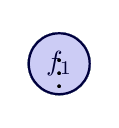
\begin{tikzpicture}[x=\figurewidth,y=\figureheight]
  \message{^^JNeural network activation}
  \def\NI{4} % number of nodes in input layers
  \def\NO{4} % number of nodes in output layers
  \def\yshift{0.4} % shift last node for dots
  
  % INPUT LAYER
  \foreach \i [evaluate={\c=int(\i==\NI); \y=\NI/2-\i-\c*\yshift; \index=(\i<\NI?int(\i):"D");}]
              in {1,...,\NI}{ % loop over nodes
    \node[node in,outer sep=0.6] (NI-\i) at (0,\y) {$u_{\index}$};
  }
  
  % OUTPUT LAYER
  \foreach \i [evaluate={\c=int(\i==\NO); \y=\NO/2-\i-\c*\yshift; \index=(\i<\NO?int(\i):"D");}]
    in {\NO,...,1}{ % loop over nodes
    \ifnum\i=1 % high-lighted node
      \node[node hidden]
        (NO-\i) at (1,\y) {$f_{\index}$};
      % \foreach \j [evaluate={\index=(\j<\NI?int(\j):"D");}] in {1,...,\NI}{ % loop over nodes in previous layer
        \draw[connect,white,line width=1.2] (NI-\i) -- (NO-\i);
        \draw[connect] (NI-\i) -- (NO-\i);
      %     % node[pos=0.50] {\contour{white}{$a_{1,\index}$}};
      % }
    \else % other light-colored nodes
      \node[node,blue!20!black!80,draw=myblue!20,fill=myblue!5]
        (NO-\i) at (1,\y) {$f_{\index}$};
      % \foreach \j in {1,...,\NI}{ % loop over nodes in previous layer
        %\draw[connect,white,line width=1.2] (NI-\j) -- (NO-\i);
        \draw[connect,myblue!20] (NI-\i) -- (NO-\i);
      % }
    \fi
  }
  
  % DOTS
  \path (NI-\NI) --++ (0,1+\yshift) node[midway,scale=1.2] {$\vdots$};
  \path (NO-\NO) --++ (0,1+\yshift) node[midway,scale=1.2] {$\vdots$};
  

  
\end{tikzpicture}
	
%		\end{column}
%		
%	\end{columns}
%\end{frame}


\begin{frame}{Linear Model of Coregionalization GP (LMCGP)}
	\centering
	\setlength\figurewidth{0.55\textwidth} 
	\setlength\figureheight{0.11\textwidth}
	% NEURAL NETWORK activation
% https://www.youtube.com/watch?v=aircAruvnKk&list=PLZHQObOWTQDNU6R1_67000Dx_ZCJB-3pi&index=1

\begin{tikzpicture}[x=\figurewidth,y=\figureheight]
  \message{^^JNeural network activation}
  \def\NI{4} % number of nodes in input layers
  \def\NO{4} % number of nodes in output layers
  \def\yshift{0.4} % shift last node for dots
  
  % INPUT LAYER
  \foreach \i [evaluate={\c=int(\i==\NI); \y=\NI/2-\i-\c*\yshift; \index=(\i<\NI?int(\i):"Q");}]
              in {1,...,\NI}{ % loop over nodes
    \node[node in,outer sep=0.6] (NI-\i) at (0,\y) {$u_{\index}$};
  }
  
  % OUTPUT LAYER
  \foreach \i [evaluate={\c=int(\i==\NO); \y=\NO/2-\i-\c*\yshift; \index=(\i<\NO?int(\i):"D");}]
    in {\NO,...,1}{ % loop over nodes
    \ifnum\i=1 % high-lighted node
      \node[node hidden]
        (NO-\i) at (1,\y) {$f_{\index}$};
      \foreach \j [evaluate={\index=(\j<\NI?int(\j):"Q");}] in {1,...,\NI}{ % loop over nodes in previous layer
        \draw[connect,white,line width=1.2] (NI-\j) -- (NO-\i);
        \draw[connect] (NI-\j) -- (NO-\i)
          node[pos=0.50] {\contour{white}{$a_{1,\index}$}};
      }
    \else % other light-colored nodes
      \node[node,blue!20!black!80,draw=myblue!20,fill=myblue!5]
        (NO-\i) at (1,\y) {$f_{\index}$};
      \foreach \j in {1,...,\NI}{ % loop over nodes in previous layer
        %\draw[connect,white,line width=1.2] (NI-\j) -- (NO-\i);
        \draw[connect,myblue!20] (NI-\j) -- (NO-\i);
      }
    \fi
  }
  
  % DOTS
  \path (NI-\NI) --++ (0,1+\yshift) node[midway,scale=1.2] {$\vdots$};
  \path (NO-\NO) --++ (0,1+\yshift) node[midway,scale=1.2] {$\vdots$};
  

  
\end{tikzpicture}

	
	\begin{columns}[T] % Top alignment

		\begin{column}{0.5\textwidth}
			\centering
	\textcolor{mygreen}{
		\textbf{Independent Process (IGP)}
		\begin{equation*}
			u_{q}(\mathbf{x}) \sim \mathcal{GP}(0, k_{q}(\mathbf{x}, \mathbf{x}'))
		\end{equation*}
	}
	\end{column}
	
	
	\begin{column}{0.5\textwidth}
		\centering
		\textcolor{myblue}{
			\textbf{Latent Process (LMCGP)}
			\begin{equation*}
				f_{d}(\mathbf{x}) = \sum_{q=1}^Q a_{d,q} u_{q}(\mathbf{x})
			\end{equation*}	
		}
	\end{column}
	
	\end{columns}
\end{frame}


\begin{frame}{Variational Inference, ELBO, and Predictive Distribution}
	We extend variational inference to include the independent set, utilizing the inducing variables $u_q$ derived from independent processes. The ELBO is given by:
	
	\begin{equation*}\label{eq:lmc_elbo}
		\mathcal{L} = \sum_{d=1}^D\sum_{n=1}^{N} \mathbb{E}_{q(f_{dn})}\{\log p(y_{dn} \mid f_{dn})\} - \sum_{q=1}^Q \text{KL}\{q(\mathbf{u}_q)\parallel p(\mathbf{u}_q)\}
	\end{equation*}
	
	The posterior over test points $X_*$, $p(\mathbf{f}_* \mid \mathbf{y})$, is given by:
	
	\begin{equation*}
		p(\mathbf{f}_* \mid \mathbf{y}) \approx q(\mathbf{f}_*) = \int p(\mathbf{f}_* \mid \mathbf{u}) q(\mathbf{u}) d \mathbf{u}
	\end{equation*}
	
	Gaussian noise $\sigma_{Nd}^2$ is added to obtain the predictive distribution.
\end{frame}

\begin{frame}{Model Setup}

	\begin{block}{Covariance Function (LMCGP)}
		The LMCGP model uses a squared exponential kernel:
		\begin{equation*}
			k_{q}\left(\mathbf{x}, \mathbf{x'} \mid \Theta_q \right) = \exp\left(-\frac{1}{2}(\mathbf{x} - \mathbf{x'})^\top \Theta_q^{-2} (\mathbf{x} - \mathbf{x'})\right)
		\end{equation*}
		Here, \( \Theta_q \) is the lengthscale matrix, and \( a_{d, q} \) work as outputscales.
	\end{block}
	
	\begin{block}{Optimization and Model Variants}
		Strong dependencies between parameters may cause poor local minima \cite{giraldo2021fully}. We address this by combining Natural Gradient (NG) to optimize variational parameters, and Adam for the rest \cite{pmlr-v84-salimbeni18a}.

		\textbf{Variants:}
		\begin{itemize}
			\item IGP: Independent GP (Adam).
			\item IGP+: Independent GP (Adam+NG).
			\item LMCGP: Correlated GP (Adam+NG)
		\end{itemize}
	\end{block}
\end{frame}



\subsection{Results and Discussions}

\subsubsection{Hyperparameter Tuning}

\begin{frame}{Performance metrics vs Q}
	\begin{figure}[htbp]
	\tiny
	\centering
	\setlength\figurewidth{0.5\columnwidth} 
	\setlength\figureheight{0.28\columnwidth}
	
	\subfloat[MSE]{% This file was created with tikzplotlib v0.10.1.
\begin{tikzpicture}

\definecolor{darkgray176}{RGB}{176,176,176}
\definecolor{steelblue31119180}{RGB}{31,119,180}

\begin{axis}[
width=\figurewidth,
height=\figureheight,
axis background/.style={fill=background_color},
axis line style={white},
tick align=inside,
tick pos=left,
x grid style={white},
y grid style={white},
xmajorgrids,
ymajorgrids,
xmin=-1.25, xmax=48.25,
xtick style={color=black},
ymin=0.259536486825269, ymax=0.731194606213278,
ytick style={color=black},
xlabel style={font=\tiny},
tick label style={font=\tiny}
]
\addplot [semithick, steelblue31119180, mark=*, mark size=1, mark options={solid}]
table {%
1 0.70975560078655
2 0.570005452889205
3 0.524956091611488
4 0.468590469300411
5 0.435353470792991
6 0.411259722878218
7 0.409096034731835
8 0.385485371917808
9 0.381016960281645
10 0.360132840745332
11 0.362921694624643
12 0.347941662750589
13 0.33894395440443
14 0.342577112243772
15 0.343123787309784
16 0.334095395016974
17 0.330290643463412
18 0.322687081772815
19 0.326757528243904
20 0.437607617331642
21 0.304623270578551
22 0.389408892826712
23 0.316685484093948
24 0.381513763041057
25 0.375840283026447
26 0.377810182111291
27 0.414747999915877
28 0.280975492251997
29 0.393662339819777
30 0.373947243132724
31 0.402964916925179
32 0.385485092508175
33 0.431905374190024
34 0.38280924563172
35 0.397469992032685
36 0.390029348756403
37 0.427310239658667
38 0.408634597214847
39 0.437765674807815
40 0.40614578730405
41 0.40052469480261
42 0.43521136441382
43 0.423471188409076
44 0.405748603781294
45 0.409759054806833
46 0.390775042857023
};
\end{axis}

\end{tikzpicture}
}\hspace{-0.1em}
	\subfloat[MSLL]{% This file was created with tikzplotlib v0.10.1.
\begin{tikzpicture}

\definecolor{darkgray176}{RGB}{176,176,176}
\definecolor{steelblue31119180}{RGB}{31,119,180}

\begin{axis}[
width=\figurewidth,
height=\figureheight,
axis background/.style={fill=background_color},
axis line style={white},
tick align=inside,
tick pos=left,
x grid style={white},
y grid style={white},
xmajorgrids,
ymajorgrids,
xmin=-1.25, xmax=48.25,
xtick style={color=black},
ymin=-1.06651615899946, ymax=-0.510154630298139,
ytick style={color=black},
xlabel={Number of Independent GPs (Q)},
xlabel style={font=\tiny},
tick label style={font=\tiny}
]
\addplot [semithick, steelblue31119180, mark=*, mark size=1, mark options={solid}]
table {%
1 -0.535443790693654
2 -0.656143802651295
3 -0.738178467100046
4 -0.800136632373368
5 -0.840255253429766
6 -0.875183228780147
7 -0.883212638166813
8 -0.916060696072918
9 -0.92732556592439
10 -0.941608614832543
11 -0.941373520408176
12 -0.963328948986684
13 -0.959595962050077
14 -0.96451770455758
15 -0.95974756275392
16 -0.971143985423901
17 -0.981752140746748
18 -0.952261104902915
19 -0.979157271636092
20 -0.642391297788161
21 -1.00087763478619
22 -0.720088184779209
23 -0.954280692847926
24 -0.728105102288219
25 -0.735847580651938
26 -0.735567459714915
27 -0.672249112260655
28 -1.04122699860395
29 -0.705361482919378
30 -0.729647651122807
31 -0.678594473020219
32 -0.711949327335191
33 -0.64218758924277
34 -0.719052195633076
35 -0.694440862143111
36 -0.703501481048209
37 -0.654029715100638
38 -0.668137210996388
39 -0.621833430969577
40 -0.671693822590583
41 -0.67987459279109
42 -0.638762954793032
43 -0.660630779693286
44 -0.675898190836243
45 -0.674508388989054
46 -0.695663541852463
};
\end{axis}

\end{tikzpicture}
}\\
	\vspace{-0.1em} % Adjust spacing between rows
	
	\subfloat[CRPS]{% This file was created with tikzplotlib v0.10.1.
\begin{tikzpicture}

\definecolor{darkgray176}{RGB}{176,176,176}
\definecolor{steelblue31119180}{RGB}{31,119,180}

\begin{axis}[
width=\figurewidth,
height=\figureheight,
axis background/.style={fill=background_color},
axis line style={white},
tick align=inside,
tick pos=left,
x grid style={white},
y grid style={white},
xmajorgrids,
ymajorgrids,
xmin=-1.25, xmax=48.25,
xtick style={color=black},
ymin=0.239929987456654, ymax=0.438839652236985,
ytick style={color=black},
xlabel style={font=\tiny},
tick label style={font=\tiny}
]
\addplot [semithick, steelblue31119180, mark=*, mark size=1, mark options={solid}]
table {%
1 0.429798303837879
2 0.374510552905612
3 0.345960005084818
4 0.323892519212847
5 0.311383175599372
6 0.299542632982873
7 0.297875424155548
8 0.28784981072712
9 0.286844690564962
10 0.279610258905049
11 0.279515690474725
12 0.273041146856969
13 0.271082282952741
14 0.271889987179417
15 0.270210632285698
16 0.26759372049199
17 0.266678895529016
18 0.264912747643612
19 0.26441644238815
20 0.309002018166923
21 0.257220132139326
22 0.291456973758776
23 0.2613559059979
24 0.287804261488934
25 0.285577216964857
26 0.287627602712463
27 0.300194088705333
28 0.24897133585576
29 0.293655299555358
30 0.287299736020118
31 0.296865072134467
32 0.291250790206968
33 0.307497232174908
34 0.289441525631671
35 0.294363581321622
36 0.291544275421493
37 0.305791393660394
38 0.296662343784081
39 0.308247437640682
40 0.298021172730888
41 0.29625972317634
42 0.307272161655389
43 0.303820351549033
44 0.297729094232099
45 0.299530085504188
46 0.293446316295075
};
\end{axis}

\end{tikzpicture}
}\hspace{-0.1em}
	\subfloat[NLPD]{% This file was created with tikzplotlib v0.10.1.
\begin{tikzpicture}

\definecolor{darkgray176}{RGB}{176,176,176}
\definecolor{steelblue31119180}{RGB}{31,119,180}

\begin{axis}[
width=\figurewidth,
height=\figureheight,
axis background/.style={fill=background_color},
axis line style={white},
tick align=inside,
tick pos=left,
x grid style={white},
y grid style={white},
xmajorgrids,
ymajorgrids,
xmin=-1.25, xmax=48.25,
xtick style={color=black},
ymin=8.86884898711136, ymax=21.6651641472417,
ytick style={color=black},
xlabel={Number of Independent GPs (Q)},
]
\addplot [semithick, steelblue31119180, mark=*, mark size=1, mark options={solid}]
table {%
1 21.0835134581449
2 18.3074131831191
3 16.4206159007979
4 14.9955780995115
5 14.0728498152143
6 13.2695063821556
7 13.0848299662623
8 12.3293246344218
9 12.070232627838
10 11.7417225029505
11 11.7471296747109
12 11.2421548174052
13 11.3280135169472
14 11.2148134392746
15 11.3245267007588
16 11.0624089793492
17 10.8184214069237
18 11.4967152313319
19 10.8781033964688
20 18.6237207949712
21 10.3785350440165
22 16.8366923941771
23 11.4502647085967
24 16.6523032914699
25 16.4742262891044
26 16.4806690706559
27 17.9369910621039
28 9.4504996762082
29 17.1754065369533
30 16.6168246682744
31 17.7910477646339
32 17.0238861153895
33 18.6284060915152
34 16.8605201445382
35 17.4265808148074
36 17.2181865799902
37 18.3560371967843
38 18.031564791182
39 19.0965517317987
40 17.9497627245155
41 17.7616050099039
42 18.7071726838592
43 18.2042127111534
44 17.8530622548654
45 17.8850276973507
46 17.3984591814923
};
\end{axis}

\end{tikzpicture}
}
	\end{figure}
	\vspace{-1em}
	\begin{block}{}
	 Beyond $Q=19$, adding more independent GPs becomes counterproductive due to handling a more complex model. We select $Q=17$ as the proper parameter.
	\end{block}
\end{frame}

\begin{frame}{Reservoir-wise Lengthscale and $a_{d, q}$}
\begin{figure}[htbp]
	\tiny
	\centering
	\setlength\figurewidth{0.4\columnwidth} 
	\setlength\figureheight{0.35\columnwidth}
	\vspace{-1.5em}
	% This file was created with tikzplotlib v0.10.1.
\begin{tikzpicture}

\definecolor{darkgray176}{RGB}{176,176,176}

\begin{axis}[
width=\figurewidth,%
height=\figureheight,%
title={$H=1$},
%colorbar,
%colorbar style={ylabel={}},
colormap/viridis,
point meta max=40,
point meta min=20,
%tick align=outside,
tick pos=left,
x grid style={darkgray176},
xmin=0, xmax=23,
xtick style={color=black},
xtick={0.5,2.5,4.5,6.5,8.5,10.5,12.5,14.5,16.5,18.5,20.5,22.5},
xticklabel style={rotate=0.0},
xticklabels={A,C,E,G,I,K,M,O,Q,S,U,W},
y dir=reverse,
y grid style={darkgray176},
ymin=0, ymax=17,
ytick style={color=black},
ytick={0.5,2.5,4.5,6.5,8.5,10.5,12.5,14.5,16.5,18.5,20.5,22.5},
yticklabel style={rotate=0.0},
yticklabels={1,3,5,7,9,11,13,15,17},
xlabel style={font=\tiny},
tick label style={font=\tiny}
]
\addplot graphics [includegraphics cmd=\pgfimage,xmin=0, xmax=23, ymin=17, ymax=0] {chp_lmc/figures/lengthscale_matrix_1-000.png};
\end{axis}

\end{tikzpicture}
 % Direct inclusion, no subcaption
	% This file was created with tikzplotlib v0.10.1.
\begin{tikzpicture}

\definecolor{darkgray176}{RGB}{176,176,176}

\begin{axis}[
width=\figurewidth,%
height=\figureheight,%
colorbar,
colorbar style={ylabel={}},
colormap/viridis,
point meta max=40,
point meta min=20,
tick align=outside,
tick pos=left,
x grid style={darkgray176},
xmin=0, xmax=23,
xtick style={color=black},
xtick={0.5,2.5,4.5,6.5,8.5,10.5,12.5,14.5,16.5,18.5,20.5,22.5},
xticklabel style={rotate=0.0},
xticklabels={A,C,E,G,I,K,M,O,Q,S,U,W},
y dir=reverse,
y grid style={darkgray176},
ymin=0, ymax=17,
ytick style={color=black},
ytick={0.5,2.5,4.5,6.5,8.5,10.5,12.5,14.5,16.5,18.5,20.5,22.5},
yticklabel style={rotate=0.0},
yticklabels={1,3,5,7,9,11,13,15,17},
xlabel style={font=\tiny},
tick label style={font=\tiny}
]
\addplot graphics [includegraphics cmd=\pgfimage,xmin=0, xmax=23, ymin=17, ymax=0] {chp_lmc/figures/lengthscale_matrix_30-000.png};
\end{axis}

\end{tikzpicture}
\\ % Direct inclusion, no subcaption
%	\vspace{-50.0em}
	% This file was created with tikzplotlib v0.10.1.
\begin{tikzpicture}

\definecolor{darkgray176}{RGB}{176,176,176}

\begin{axis}[
width=\figurewidth,%
height=\figureheight,%
colorbar,
colorbar style={ylabel={}},
colormap/viridis,
point meta max=1.5,
point meta min=0,
tick align=outside,
tick pos=left,
x grid style={darkgray176},
xmin=0, xmax=17,
xtick style={color=black},
xtick={0.5,2.5,4.5,6.5,8.5,10.5,12.5,14.5,16.5,18.5,20.5,22.5},
xticklabel style={rotate=0.0},
xticklabels={1,3,5,7,9,11,13,15,17},
y dir=reverse,
y grid style={darkgray176},
ymin=0, ymax=23,
ytick style={color=black},
ytick={0.5,2.5,4.5,6.5,8.5,10.5,12.5,14.5,16.5,18.5,20.5,22.5},
yticklabel style={rotate=0.0},
yticklabels={A,C,E,G,I,K,M,O,Q,S,U,W},
]
\addplot graphics [includegraphics cmd=\pgfimage,xmin=0, xmax=17, ymin=23, ymax=0] {chp_lmc/figures/coregionalization_1-000.png};
\end{axis}

\end{tikzpicture}
 % Direct inclusion, no subcaption
	% This file was created with tikzplotlib v0.10.1.
\begin{tikzpicture}

\definecolor{darkgray176}{RGB}{176,176,176}

\begin{axis}[
width=\figurewidth,%
height=\figureheight,%
colorbar,
colorbar style={ylabel={}},
colormap/viridis,
point meta max=1.5,
point meta min=0,
tick align=outside,
tick pos=left,
x grid style={darkgray176},
xmin=0, xmax=17,
xtick style={color=black},
xtick={0.5,2.5,4.5,6.5,8.5,10.5,12.5,14.5,16.5,18.5,20.5,22.5},
xticklabel style={rotate=0.0},
xticklabels={1,3,5,7,9,11,13,15,17},
y dir=reverse,
y grid style={darkgray176},
ymin=0, ymax=23,
ytick style={color=black},
ytick={0.5,2.5,4.5,6.5,8.5,10.5,12.5,14.5,16.5,18.5,20.5,22.5},
yticklabel style={rotate=0.0},
yticklabels={A,C,E,G,I,K,M,O,Q,S,U,W},
xlabel style={font=\tiny},
tick label style={font=\tiny}
]
\addplot graphics [includegraphics cmd=\pgfimage,xmin=0, xmax=17, ymin=23, ymax=0] {chp_lmc/figures/coregionalization_30-000.png};
\end{axis}

\end{tikzpicture}
 % Direct inclusion, no subcaption
\end{figure}


	\vspace{-1.0em}
	\begin{block}{}
		Increase horizon, lengthscale values show less selective. All independent GPs incorporate more features due to the extended time gap. The $a_{d,q}$ coefficients are smaller, indicating weaker individual feature contributions to each output.
	\end{block}
	
	
\end{frame}


\subsubsection{Performance Analysis}

\begin{frame}{Bar plots comparing IGP, IGP+, and LMCGP}
	\begin{figure}[htbp]
		\centering
		\setlength\figurewidth{0.56\columnwidth}
		\setlength\figureheight{0.48\columnwidth}
		
		\subfloat[MSLL]{% This file was created with tikzplotlib v0.10.1.
\begin{tikzpicture}

\definecolor{darkgray176}{RGB}{176,176,176}
\definecolor{gray}{RGB}{128,128,128}
\definecolor{green01270}{RGB}{0,127,0}
\definecolor{lightgray204}{RGB}{204,204,204}

\begin{axis}[
width=\figurewidth,%
height=\figureheight,%
axis background/.style={fill=background_color},
tick align=outside,
tick pos=left,
axis line style={white},
tick align=inside,
tick pos=left,
x grid style={white},
y grid style={white},
xmajorgrids,
ymajorgrids,
xlabel={Horizon},
xmin=-0.6125, xmax=10.1125,
xtick style={color=black},
xtick={0.25,1.25,2.25,3.25,4.25,5.25,6.25,7.25,8.25,9.25},
xticklabels={1,2,3,4,5,6,7,14,21,30},
ymin=-1.03083974778409, ymax=0,
ytick style={color=black},
legend columns=3, 
legend style={
  nodes={scale=0.8, transform shape},
  fill opacity=1,
  draw opacity=1,
  text opacity=1,
  at={(0.03,0.97)},
  anchor=north west,
  legend pos=north west,
  draw=lightgray204,
  fill=background_color,
  font=\tiny
},
xlabel style={font=\tiny},
tick label style={font=\tiny}
]
\draw[draw=gray,fill=blue] (axis cs:-0.125,0) rectangle (axis cs:0.125,-0.532252569204355);
\addlegendimage{ybar,ybar legend,draw=gray,fill=blue}
\addlegendentry{IGP}

\draw[draw=gray,fill=blue] (axis cs:0.875,0) rectangle (axis cs:1.125,-0.428154570305303);
\draw[draw=gray,fill=blue] (axis cs:1.875,0) rectangle (axis cs:2.125,-0.388555233274582);
\draw[draw=gray,fill=blue] (axis cs:2.875,0) rectangle (axis cs:3.125,-0.351859932002441);
\draw[draw=gray,fill=blue] (axis cs:3.875,0) rectangle (axis cs:4.125,-0.332820583869734);
\draw[draw=gray,fill=blue] (axis cs:4.875,0) rectangle (axis cs:5.125,-0.327618686894435);
\draw[draw=gray,fill=blue] (axis cs:5.875,0) rectangle (axis cs:6.125,-0.316243282995642);
\draw[draw=gray,fill=blue] (axis cs:6.875,0) rectangle (axis cs:7.125,-0.272667322281103);
\draw[draw=gray,fill=blue] (axis cs:7.875,0) rectangle (axis cs:8.125,-0.238004115713702);
\draw[draw=gray,fill=blue] (axis cs:8.875,0) rectangle (axis cs:9.125,-0.209382344201211);
\draw[draw=gray,fill=green01270] (axis cs:0.125,0) rectangle (axis cs:0.375,-0.941880236439821);
\addlegendimage{ybar,ybar legend,draw=gray,fill=green01270}
\addlegendentry{IGP+}

\draw[draw=gray,fill=green01270] (axis cs:1.125,0) rectangle (axis cs:1.375,-0.823059544090509);
\draw[draw=gray,fill=green01270] (axis cs:2.125,0) rectangle (axis cs:2.375,-0.795239515783919);
\draw[draw=gray,fill=green01270] (axis cs:3.125,0) rectangle (axis cs:3.375,-0.763465923433985);
\draw[draw=gray,fill=green01270] (axis cs:4.125,0) rectangle (axis cs:4.375,-0.768541284578963);
\draw[draw=gray,fill=green01270] (axis cs:5.125,0) rectangle (axis cs:5.375,-0.745977231234278);
\draw[draw=gray,fill=green01270] (axis cs:6.125,0) rectangle (axis cs:6.375,-0.750924112092601);
\draw[draw=gray,fill=green01270] (axis cs:7.125,0) rectangle (axis cs:7.375,-0.733609018426772);
\draw[draw=gray,fill=green01270] (axis cs:8.125,0) rectangle (axis cs:8.375,-0.699696669917477);
\draw[draw=gray,fill=green01270] (axis cs:9.125,0) rectangle (axis cs:9.375,-0.704798766364212);
\draw[draw=gray,fill=red] (axis cs:0.375,0) rectangle (axis cs:0.625,-0.981752140746748);
\addlegendimage{ybar,ybar legend,draw=gray,fill=red}
\addlegendentry{LMCGP}

\draw[draw=gray,fill=red] (axis cs:1.375,0) rectangle (axis cs:1.625,-0.908594506349704);
\draw[draw=gray,fill=red] (axis cs:2.375,0) rectangle (axis cs:2.625,-0.86460885583022);
\draw[draw=gray,fill=red] (axis cs:3.375,0) rectangle (axis cs:3.625,-0.848106883276553);
\draw[draw=gray,fill=red] (axis cs:4.375,0) rectangle (axis cs:4.625,-0.856711145565708);
\draw[draw=gray,fill=red] (axis cs:5.375,0) rectangle (axis cs:5.625,-0.81889702921591);
\draw[draw=gray,fill=red] (axis cs:6.375,0) rectangle (axis cs:6.625,-0.857418455961666);
\draw[draw=gray,fill=red] (axis cs:7.375,0) rectangle (axis cs:7.625,-0.827809320362084);
\draw[draw=gray,fill=red] (axis cs:8.375,0) rectangle (axis cs:8.625,-0.816824060358377);
\draw[draw=gray,fill=red] (axis cs:9.375,0) rectangle (axis cs:9.625,-0.798021526304375);
\end{axis}

\end{tikzpicture}
}
		\hfill
		\subfloat[NLPD]{% This file was created with tikzplotlib v0.10.1.
\begin{tikzpicture}

\definecolor{darkgray176}{RGB}{176,176,176}
\definecolor{gray}{RGB}{128,128,128}
\definecolor{green01270}{RGB}{0,127,0}

\begin{axis}[
width=\figurewidth,%
height=\figureheight,%
axis background/.style={fill=background_color},
tick align=outside,
tick pos=left,
axis line style={white},
tick align=inside,
tick pos=left,
x grid style={white},
y grid style={white},
xmajorgrids,
ymajorgrids,
xlabel={Horizon},
xtick style={color=black},
xtick={0.25,1.25,2.25,3.25,4.25,5.25,6.25,7.25,8.25,9.25},
xticklabels={1,2,3,4,5,6,7,14,21,30},
ytick style={color=black},
xmin=-0.6125, xmax=10.1125,
ymin=0, ymax=29.8449605648958,
xlabel style={font=\tiny},
tick label style={font=\tiny}
]
\draw[draw=gray,fill=blue] (axis cs:-0.125,0) rectangle (axis cs:0.125,21.1569115523988);
\draw[draw=gray,fill=blue] (axis cs:0.875,0) rectangle (axis cs:1.125,23.5500376665929);
\draw[draw=gray,fill=blue] (axis cs:1.875,0) rectangle (axis cs:2.125,24.4596859590331);
\draw[draw=gray,fill=blue] (axis cs:2.875,0) rectangle (axis cs:3.125,25.3025311179923);
\draw[draw=gray,fill=blue] (axis cs:3.875,0) rectangle (axis cs:4.125,25.7392946447281);
\draw[draw=gray,fill=blue] (axis cs:4.875,0) rectangle (axis cs:5.125,25.8577961476045);
\draw[draw=gray,fill=blue] (axis cs:5.875,0) rectangle (axis cs:6.125,26.1182370685187);
\draw[draw=gray,fill=blue] (axis cs:6.875,0) rectangle (axis cs:7.125,27.0243046679054);
\draw[draw=gray,fill=blue] (axis cs:7.875,0) rectangle (axis cs:8.125,27.7866695852108);
\draw[draw=gray,fill=blue] (axis cs:8.875,0) rectangle (axis cs:9.125,28.4237719665674);
\draw[draw=gray,fill=green01270] (axis cs:0.125,0) rectangle (axis cs:0.375,11.7354752059831);

\draw[draw=gray,fill=green01270] (axis cs:1.125,0) rectangle (axis cs:1.375,14.4672232695331);
\draw[draw=gray,fill=green01270] (axis cs:2.125,0) rectangle (axis cs:2.375,15.1059474613183);
\draw[draw=gray,fill=green01270] (axis cs:3.125,0) rectangle (axis cs:3.375,15.8355933150668);
\draw[draw=gray,fill=green01270] (axis cs:4.125,0) rectangle (axis cs:4.375,15.7177185284159);
\draw[draw=gray,fill=green01270] (axis cs:5.125,0) rectangle (axis cs:5.375,16.2355496277881);
\draw[draw=gray,fill=green01270] (axis cs:6.125,0) rectangle (axis cs:6.375,16.1205779992887);
\draw[draw=gray,fill=green01270] (axis cs:7.125,0) rectangle (axis cs:7.375,16.4226456565551);
\draw[draw=gray,fill=green01270] (axis cs:8.125,0) rectangle (axis cs:8.375,17.167740838524);
\draw[draw=gray,fill=green01270] (axis cs:9.125,0) rectangle (axis cs:9.375,17.0291942568183);
\draw[draw=gray,fill=red] (axis cs:0.375,0) rectangle (axis cs:0.625,10.8184214069237);

\draw[draw=gray,fill=red] (axis cs:1.375,0) rectangle (axis cs:1.625,12.4999191375716);
\draw[draw=gray,fill=red] (axis cs:2.375,0) rectangle (axis cs:2.625,13.5104526402534);
\draw[draw=gray,fill=red] (axis cs:3.375,0) rectangle (axis cs:3.625,13.8888512386877);
\draw[draw=gray,fill=red] (axis cs:4.375,0) rectangle (axis cs:4.625,13.6898117257208);
\draw[draw=gray,fill=red] (axis cs:5.375,0) rectangle (axis cs:5.625,14.5583942742105);
\draw[draw=gray,fill=red] (axis cs:6.375,0) rectangle (axis cs:6.625,13.6712080903002);
\draw[draw=gray,fill=red] (axis cs:7.375,0) rectangle (axis cs:7.625,14.2560387120429);
\draw[draw=gray,fill=red] (axis cs:8.375,0) rectangle (axis cs:8.625,14.4738108583833);
\draw[draw=gray,fill=red] (axis cs:9.375,0) rectangle (axis cs:9.625,14.8850707781946);
\end{axis}

\end{tikzpicture}
}
		
	\end{figure}
	\vspace{-2.0em}
	\begin{block}{}
		The Adam+NG optimizer significantly boosts performance, and with LMCGP showing the most improvement, especially for larger horizons.
	\end{block}
	
	
\end{frame}

%\begin{frame}{Model Forecasting}
%	\centering
%	\begin{figure}[htbp]
%	\tiny
%	\setlength\figurewidth{0.55\columnwidth} 
%	\setlength\figureheight{0.5\columnwidth}
%
%	\subfloat[$A$.]{% This file was created with tikzplotlib v0.10.1.
\begin{tikzpicture}

\definecolor{darkgray176}{RGB}{176,176,176}

\begin{axis}[
width=\figurewidth,
height=\figureheight,
axis background/.style={fill=background_color},
axis line style={white},
tick align=inside,
tick pos=left,
ylabel={Contributions (kWh)},
x grid style={white},
xmajorgrids,
xmin=50, xmax=200,
xtick style={color=black},
y grid style={white},
ymajorgrids,
ymin=-3414130.1187411, ymax=12497779.277438,
ytick style={color=black},
ytick={-4000000,-2000000,0,2000000,4000000,6000000,8000000,10000000,12000000,14000000},
]
\path [draw=blue, fill=blue, opacity=0.5]
(axis cs:0,7679984.24705729)
--(axis cs:0,2917489.43104134)
--(axis cs:1,2982475.2004108)
--(axis cs:2,3412409.28949479)
--(axis cs:3,3203869.38989402)
--(axis cs:4,2912864.85847748)
--(axis cs:5,3294361.27001976)
--(axis cs:6,2504446.52562919)
--(axis cs:7,2455496.5359375)
--(axis cs:8,2063730.61385061)
--(axis cs:9,2471527.08738114)
--(axis cs:10,2087061.93914864)
--(axis cs:11,2068758.04016285)
--(axis cs:12,1653180.33918535)
--(axis cs:13,3859736.02751677)
--(axis cs:14,4537897.20831926)
--(axis cs:15,3277620.00039835)
--(axis cs:16,1695284.85875567)
--(axis cs:17,1966959.62473449)
--(axis cs:18,3134134.78771934)
--(axis cs:19,2828709.56750116)
--(axis cs:20,3876449.59478391)
--(axis cs:21,2848093.35253936)
--(axis cs:22,3600507.52062665)
--(axis cs:23,3022347.70935306)
--(axis cs:24,2905676.13474874)
--(axis cs:25,2481211.30106356)
--(axis cs:26,2564268.35362987)
--(axis cs:27,2030429.25208577)
--(axis cs:28,2294638.86030943)
--(axis cs:29,3322096.97925028)
--(axis cs:30,2397133.9884203)
--(axis cs:31,2053047.60767589)
--(axis cs:32,2311818.05999175)
--(axis cs:33,2697391.55598018)
--(axis cs:34,2157240.38803831)
--(axis cs:35,2401106.17088506)
--(axis cs:36,2299723.00322058)
--(axis cs:37,3800216.20377714)
--(axis cs:38,3703461.88262605)
--(axis cs:39,3019779.81502086)
--(axis cs:40,3413201.44657928)
--(axis cs:41,2881025.07959644)
--(axis cs:42,4291389.08062548)
--(axis cs:43,4060142.8237833)
--(axis cs:44,3481997.07579305)
--(axis cs:45,3891492.14582372)
--(axis cs:46,4110304.48482329)
--(axis cs:47,3532827.15842848)
--(axis cs:48,3634901.65677719)
--(axis cs:49,2869282.93787973)
--(axis cs:50,4494561.93350498)
--(axis cs:51,3216161.45753051)
--(axis cs:52,4034747.58598494)
--(axis cs:53,3317984.37464376)
--(axis cs:54,3594001.88822107)
--(axis cs:55,3117094.45043948)
--(axis cs:56,3065348.27955064)
--(axis cs:57,4650171.09004554)
--(axis cs:58,3310559.73327812)
--(axis cs:59,2809454.99209545)
--(axis cs:60,2996747.62458147)
--(axis cs:61,2426189.79359569)
--(axis cs:62,2813148.52216307)
--(axis cs:63,2811657.34525501)
--(axis cs:64,3335729.43511588)
--(axis cs:65,2537340.37919239)
--(axis cs:66,2164190.19690098)
--(axis cs:67,1654852.02503031)
--(axis cs:68,1399690.08274928)
--(axis cs:69,1237163.36781349)
--(axis cs:70,1209226.19800315)
--(axis cs:71,1436966.65871377)
--(axis cs:72,3513173.94671417)
--(axis cs:73,2820010.91609189)
--(axis cs:74,2353687.92180664)
--(axis cs:75,1902465.34870207)
--(axis cs:76,1624368.23086607)
--(axis cs:77,2095649.46641945)
--(axis cs:78,1574748.80152594)
--(axis cs:79,1683137.36360548)
--(axis cs:80,1229993.81825738)
--(axis cs:81,1066761.80772511)
--(axis cs:82,3111364.08941993)
--(axis cs:83,1701936.78221748)
--(axis cs:84,1831707.83885457)
--(axis cs:85,2562040.28739348)
--(axis cs:86,3113548.58271729)
--(axis cs:87,1877180.53775377)
--(axis cs:88,2281224.20268079)
--(axis cs:89,2586727.81812645)
--(axis cs:90,1952498.79589295)
--(axis cs:91,1802213.10017979)
--(axis cs:92,1288777.44523775)
--(axis cs:93,1105400.53027211)
--(axis cs:94,1120194.97881654)
--(axis cs:95,1275151.52814121)
--(axis cs:96,935119.511475899)
--(axis cs:97,2125290.88469931)
--(axis cs:98,2730128.1621721)
--(axis cs:99,2341227.18780366)
--(axis cs:100,1493226.36825061)
--(axis cs:101,1161461.47985358)
--(axis cs:102,1129224.43332816)
--(axis cs:103,1059155.30887248)
--(axis cs:104,1341415.34656189)
--(axis cs:105,983744.755914505)
--(axis cs:106,1664866.5549998)
--(axis cs:107,2420746.70900163)
--(axis cs:108,1655608.96741228)
--(axis cs:109,1695656.71105454)
--(axis cs:110,1453713.18470758)
--(axis cs:111,605962.766181772)
--(axis cs:112,1163845.7545825)
--(axis cs:113,577191.472753175)
--(axis cs:114,1516529.69718251)
--(axis cs:115,3358582.923284)
--(axis cs:116,2702482.98495262)
--(axis cs:117,2015092.41675752)
--(axis cs:118,1997318.90056699)
--(axis cs:119,1965145.60743524)
--(axis cs:120,2010626.58147187)
--(axis cs:121,1299869.15564852)
--(axis cs:122,1532434.83647141)
--(axis cs:123,2135592.4581391)
--(axis cs:124,2314684.70553052)
--(axis cs:125,2846091.68720357)
--(axis cs:126,2305832.55878519)
--(axis cs:127,2467803.82965228)
--(axis cs:128,1921492.81952138)
--(axis cs:129,2458008.96321451)
--(axis cs:130,2325944.66787883)
--(axis cs:131,2429545.75979456)
--(axis cs:132,1815136.82704659)
--(axis cs:133,2264282.25902703)
--(axis cs:134,2786897.04742897)
--(axis cs:135,1242794.96059963)
--(axis cs:136,1365941.21273608)
--(axis cs:137,1553723.35083154)
--(axis cs:138,1289906.37631477)
--(axis cs:139,788932.163283331)
--(axis cs:140,940767.004119291)
--(axis cs:141,1105773.15870677)
--(axis cs:142,1851531.81487777)
--(axis cs:143,1980425.71421969)
--(axis cs:144,2270204.48383211)
--(axis cs:145,2405585.91819742)
--(axis cs:146,1675951.01406862)
--(axis cs:147,1429079.19995716)
--(axis cs:148,3332519.62155422)
--(axis cs:149,1970398.27253148)
--(axis cs:150,2212308.53497331)
--(axis cs:151,731321.690293832)
--(axis cs:152,742401.862329931)
--(axis cs:153,696481.653166119)
--(axis cs:154,844265.149900103)
--(axis cs:155,965383.799802638)
--(axis cs:156,1448044.83825602)
--(axis cs:157,1038315.64862774)
--(axis cs:158,2121144.6338735)
--(axis cs:159,1381243.99103028)
--(axis cs:160,1617778.68211952)
--(axis cs:161,1290676.22403618)
--(axis cs:162,1594225.52892163)
--(axis cs:163,1180084.83564248)
--(axis cs:164,1263719.17512619)
--(axis cs:165,1232759.83590769)
--(axis cs:166,2241237.79852954)
--(axis cs:167,2547958.48127936)
--(axis cs:168,3979832.30590487)
--(axis cs:169,2684384.55364342)
--(axis cs:170,3287709.67916509)
--(axis cs:171,3432549.29471511)
--(axis cs:172,3448630.89848808)
--(axis cs:173,3017009.45836024)
--(axis cs:174,2746960.6610996)
--(axis cs:175,2735298.36892186)
--(axis cs:176,3064884.2230575)
--(axis cs:177,3645100.07441874)
--(axis cs:178,2753781.31003333)
--(axis cs:179,2463743.76010546)
--(axis cs:180,1904047.78126948)
--(axis cs:181,2267442.74088608)
--(axis cs:182,2062314.14372937)
--(axis cs:183,2132300.28432497)
--(axis cs:184,3747428.53643517)
--(axis cs:185,4033076.96487381)
--(axis cs:186,3605624.41010253)
--(axis cs:187,2356068.7823238)
--(axis cs:188,2976651.89941397)
--(axis cs:189,2440791.2162352)
--(axis cs:190,2306345.2306331)
--(axis cs:191,3351800.0534161)
--(axis cs:192,2261309.62684204)
--(axis cs:193,1819279.53589965)
--(axis cs:194,1464569.85686153)
--(axis cs:195,1698819.78271284)
--(axis cs:196,2188578.81351247)
--(axis cs:197,2694323.45912929)
--(axis cs:198,3474396.36982183)
--(axis cs:199,2938411.45915798)
--(axis cs:200,3869974.85491382)
--(axis cs:201,3120349.86858124)
--(axis cs:202,2683422.49830802)
--(axis cs:203,3724868.45667511)
--(axis cs:204,3245032.53837236)
--(axis cs:205,2132785.10054987)
--(axis cs:206,2974878.85806041)
--(axis cs:207,3196914.03575752)
--(axis cs:208,4199883.83119749)
--(axis cs:209,3451290.728535)
--(axis cs:210,3105455.07919413)
--(axis cs:211,3128299.23365977)
--(axis cs:212,2433218.17485911)
--(axis cs:213,2769390.67800514)
--(axis cs:214,3050205.51425521)
--(axis cs:215,2879942.76903341)
--(axis cs:216,2537096.49545219)
--(axis cs:217,1821998.67525135)
--(axis cs:218,1294846.54573787)
--(axis cs:219,2022770.21523863)
--(axis cs:220,1550706.08933325)
--(axis cs:221,689285.743333825)
--(axis cs:222,1123458.94219666)
--(axis cs:223,2091519.73641097)
--(axis cs:224,2221600.6607308)
--(axis cs:225,2588898.8711105)
--(axis cs:226,2063643.09785299)
--(axis cs:227,1802367.97327628)
--(axis cs:228,1249671.50296711)
--(axis cs:229,736612.423290445)
--(axis cs:230,102494.637866587)
--(axis cs:231,75155.2371517671)
--(axis cs:232,-145397.268552344)
--(axis cs:233,494222.041646762)
--(axis cs:234,616546.236871024)
--(axis cs:235,342706.927493482)
--(axis cs:236,159769.545503355)
--(axis cs:237,112298.063791818)
--(axis cs:238,-391148.456104159)
--(axis cs:239,-504510.593138072)
--(axis cs:240,372555.188068123)
--(axis cs:241,922619.762367975)
--(axis cs:242,-498242.310442616)
--(axis cs:243,-834211.405757753)
--(axis cs:244,-544254.336859646)
--(axis cs:245,-261888.349011427)
--(axis cs:246,257954.199219426)
--(axis cs:247,-196752.683902787)
--(axis cs:248,-1064551.72945586)
--(axis cs:249,-1060880.93599958)
--(axis cs:250,-788384.100683442)
--(axis cs:251,-1418055.27242892)
--(axis cs:252,-1190275.53927862)
--(axis cs:253,-978849.892340882)
--(axis cs:254,-817894.323294024)
--(axis cs:255,-58360.6458918303)
--(axis cs:256,-418422.068856314)
--(axis cs:257,-286019.019800927)
--(axis cs:258,-675867.655906836)
--(axis cs:259,-566296.756191047)
--(axis cs:260,-1617590.49495109)
--(axis cs:261,-1100575.73697092)
--(axis cs:262,-768917.460955109)
--(axis cs:263,-1671845.75501035)
--(axis cs:264,-1352822.13736866)
--(axis cs:265,-1315059.16599414)
--(axis cs:266,-1200662.26779044)
--(axis cs:267,-1192114.44657334)
--(axis cs:268,-1009209.38367926)
--(axis cs:269,-251308.632440381)
--(axis cs:270,269169.755357018)
--(axis cs:271,-961498.785289288)
--(axis cs:272,-1024219.01019484)
--(axis cs:273,1115751.80977258)
--(axis cs:274,1077096.35865129)
--(axis cs:275,2807879.67676026)
--(axis cs:276,1773298.47465474)
--(axis cs:277,3209451.75713373)
--(axis cs:278,1967719.89400045)
--(axis cs:279,2417301.04230861)
--(axis cs:280,2822802.70517876)
--(axis cs:281,3081151.00053684)
--(axis cs:282,2550851.12953923)
--(axis cs:283,1682341.6431942)
--(axis cs:284,2367219.44165324)
--(axis cs:285,2592886.59713286)
--(axis cs:286,2225712.97144436)
--(axis cs:287,2481842.45757226)
--(axis cs:288,2055939.50134904)
--(axis cs:289,2560241.14735253)
--(axis cs:290,2011428.63100231)
--(axis cs:291,1592480.28189806)
--(axis cs:292,2724382.7163194)
--(axis cs:293,2054264.09948943)
--(axis cs:294,1891202.54059085)
--(axis cs:295,1501417.80656133)
--(axis cs:296,1293635.38956902)
--(axis cs:297,998888.85364853)
--(axis cs:298,1687795.56441785)
--(axis cs:299,1156354.96763287)
--(axis cs:300,2045969.09083358)
--(axis cs:301,1309088.90913885)
--(axis cs:302,1346530.20706875)
--(axis cs:303,583675.187761881)
--(axis cs:304,423265.493671787)
--(axis cs:305,444675.38511499)
--(axis cs:306,1027462.28289674)
--(axis cs:307,1276332.78455816)
--(axis cs:308,667446.147486211)
--(axis cs:309,441178.537505197)
--(axis cs:310,361036.530339733)
--(axis cs:311,359848.942644017)
--(axis cs:312,388001.013866929)
--(axis cs:313,2120319.55307975)
--(axis cs:314,3532925.51091316)
--(axis cs:315,1668211.78606755)
--(axis cs:316,1189355.03839513)
--(axis cs:317,774533.518755079)
--(axis cs:318,484053.943311654)
--(axis cs:319,431951.171165565)
--(axis cs:320,452226.455621021)
--(axis cs:321,646648.558764158)
--(axis cs:322,656320.749266473)
--(axis cs:323,824994.071183939)
--(axis cs:324,1664474.82067434)
--(axis cs:325,1420105.02429988)
--(axis cs:326,1443991.67860116)
--(axis cs:327,1943207.27550379)
--(axis cs:328,672602.616723479)
--(axis cs:329,59565.213614882)
--(axis cs:330,972909.308632754)
--(axis cs:331,1928137.10569285)
--(axis cs:332,1367180.63002391)
--(axis cs:333,2496436.94992171)
--(axis cs:334,1646695.27865691)
--(axis cs:335,1746751.84391372)
--(axis cs:336,1716044.32219471)
--(axis cs:337,1660888.20296363)
--(axis cs:338,1730947.72984214)
--(axis cs:339,1493665.66778162)
--(axis cs:340,1290860.94633602)
--(axis cs:341,1674580.04091971)
--(axis cs:342,1002324.79565706)
--(axis cs:343,801582.916510339)
--(axis cs:344,1853343.79561231)
--(axis cs:345,1590230.56587636)
--(axis cs:346,1381269.06669185)
--(axis cs:347,1507060.94565381)
--(axis cs:348,2325146.24438242)
--(axis cs:349,2345382.89679721)
--(axis cs:350,2174982.0761801)
--(axis cs:351,2190262.48084903)
--(axis cs:352,2014551.65643376)
--(axis cs:353,2645309.35506452)
--(axis cs:354,2125941.13618584)
--(axis cs:355,2220225.50154373)
--(axis cs:356,2704948.47310419)
--(axis cs:357,3159007.19823957)
--(axis cs:358,2433518.07616621)
--(axis cs:359,2059444.41484432)
--(axis cs:360,2064578.35051255)
--(axis cs:361,2151582.14322951)
--(axis cs:362,2693986.49320545)
--(axis cs:363,3315718.48649008)
--(axis cs:364,2856572.253689)
--(axis cs:365,3439388.09630195)
--(axis cs:366,1940223.42255239)
--(axis cs:367,2272070.3962789)
--(axis cs:368,3117417.83929134)
--(axis cs:369,2332994.13105902)
--(axis cs:370,3146596.38026869)
--(axis cs:371,3468065.85506536)
--(axis cs:372,4086706.28704517)
--(axis cs:373,3759930.65356188)
--(axis cs:374,3391430.10968748)
--(axis cs:375,4034443.79796314)
--(axis cs:376,3959819.23371528)
--(axis cs:377,4235317.34346317)
--(axis cs:378,4137485.1030638)
--(axis cs:379,3496015.34363113)
--(axis cs:380,2181152.63113452)
--(axis cs:381,3092585.75026244)
--(axis cs:382,3868144.3505766)
--(axis cs:383,4011925.16037722)
--(axis cs:384,3172547.53836776)
--(axis cs:385,3890018.75265465)
--(axis cs:386,3772780.42133329)
--(axis cs:387,3254358.07719239)
--(axis cs:388,3362255.26897569)
--(axis cs:389,3492707.89090529)
--(axis cs:390,3166640.42813365)
--(axis cs:391,2892856.89934353)
--(axis cs:392,4092752.53567151)
--(axis cs:393,3771200.82051161)
--(axis cs:394,4646147.65032412)
--(axis cs:395,4364989.99027751)
--(axis cs:396,3506508.07958188)
--(axis cs:397,3323581.45236484)
--(axis cs:398,2812454.85617854)
--(axis cs:399,3998005.03209272)
--(axis cs:400,3582073.38247949)
--(axis cs:401,3763943.21289781)
--(axis cs:402,2834831.10336599)
--(axis cs:403,3506516.10781756)
--(axis cs:404,4311980.64557083)
--(axis cs:405,4283312.42445459)
--(axis cs:406,4042480.6427551)
--(axis cs:407,3340675.95059722)
--(axis cs:408,3279738.95930303)
--(axis cs:409,4198697.81156371)
--(axis cs:410,3524230.56256518)
--(axis cs:411,3050900.49603025)
--(axis cs:412,3960144.5076375)
--(axis cs:413,3613529.19174047)
--(axis cs:414,4048265.56227727)
--(axis cs:415,4317130.13664659)
--(axis cs:416,3474861.10805085)
--(axis cs:417,3519516.34854784)
--(axis cs:418,3138067.57331856)
--(axis cs:419,2803690.17493645)
--(axis cs:420,2348548.99812738)
--(axis cs:421,2263872.12187547)
--(axis cs:422,2237429.69808405)
--(axis cs:423,2851102.42285992)
--(axis cs:424,2431060.61794783)
--(axis cs:425,2043255.3426351)
--(axis cs:426,1875798.78806705)
--(axis cs:427,1980876.27960109)
--(axis cs:428,1074587.97042321)
--(axis cs:429,1194882.20566753)
--(axis cs:430,1448647.15581405)
--(axis cs:431,3885615.18217673)
--(axis cs:432,2395431.24552416)
--(axis cs:433,1726188.80308921)
--(axis cs:434,1518835.88124687)
--(axis cs:435,1369885.93183798)
--(axis cs:436,3963059.87060979)
--(axis cs:437,3867796.84753531)
--(axis cs:438,3174165.87244418)
--(axis cs:439,4290185.78046883)
--(axis cs:440,3256120.16507369)
--(axis cs:440,8022356.31003915)
--(axis cs:440,8022356.31003915)
--(axis cs:439,9691203.45842095)
--(axis cs:438,7866419.53012419)
--(axis cs:437,8710386.69306469)
--(axis cs:436,8729814.6984532)
--(axis cs:435,6064181.06058305)
--(axis cs:434,6210636.1558785)
--(axis cs:433,6410236.85286229)
--(axis cs:432,7076933.46019765)
--(axis cs:431,8597866.44141556)
--(axis cs:430,6147228.07995845)
--(axis cs:429,5897067.85148066)
--(axis cs:428,5855273.49397249)
--(axis cs:427,6691312.28447242)
--(axis cs:426,6595059.88172283)
--(axis cs:425,6820851.89778449)
--(axis cs:424,7161416.94647428)
--(axis cs:423,7551280.76531755)
--(axis cs:422,6948631.19252782)
--(axis cs:421,7048335.28621586)
--(axis cs:420,7133489.86256111)
--(axis cs:419,7541349.78049977)
--(axis cs:418,7850287.46441707)
--(axis cs:417,8258372.3385759)
--(axis cs:416,8176402.06116528)
--(axis cs:415,9038374.97633848)
--(axis cs:414,8740661.28399606)
--(axis cs:413,8308951.35332157)
--(axis cs:412,8741203.63788666)
--(axis cs:411,7745851.07282461)
--(axis cs:410,8210095.86799942)
--(axis cs:409,8970816.99739047)
--(axis cs:408,7955101.18326571)
--(axis cs:407,8024635.58924367)
--(axis cs:406,8746584.26977279)
--(axis cs:405,9263590.65680052)
--(axis cs:404,9163335.29814785)
--(axis cs:403,8241139.79166751)
--(axis cs:402,7536376.66274259)
--(axis cs:401,8474613.8239344)
--(axis cs:400,8267840.11074639)
--(axis cs:399,8690879.77504601)
--(axis cs:398,7500819.66104002)
--(axis cs:397,8028173.07387978)
--(axis cs:396,8344917.75035064)
--(axis cs:395,9512468.64800802)
--(axis cs:394,9672833.67191725)
--(axis cs:393,8527351.07688676)
--(axis cs:392,8829111.93168207)
--(axis cs:391,7563055.79117382)
--(axis cs:390,7882167.05603462)
--(axis cs:389,8171488.55926914)
--(axis cs:388,8044000.56481757)
--(axis cs:387,7980366.180205)
--(axis cs:386,8470653.80442838)
--(axis cs:385,8595415.37318593)
--(axis cs:384,7901820.00849699)
--(axis cs:383,8741656.22342907)
--(axis cs:382,8592232.92436555)
--(axis cs:381,7800415.71810708)
--(axis cs:380,7110305.73232726)
--(axis cs:379,8460103.66663251)
--(axis cs:378,9200822.92396957)
--(axis cs:377,9124663.08237261)
--(axis cs:376,8864320.06526396)
--(axis cs:375,8750093.95695064)
--(axis cs:374,8082852.41242962)
--(axis cs:373,8453698.03346741)
--(axis cs:372,8839859.85695364)
--(axis cs:371,8185143.61466612)
--(axis cs:370,7821365.91307012)
--(axis cs:369,7017415.705728)
--(axis cs:368,7807572.4543371)
--(axis cs:367,6998019.46415688)
--(axis cs:366,6845152.37655341)
--(axis cs:365,8136843.28837586)
--(axis cs:364,7601084.20756068)
--(axis cs:363,8027974.65681743)
--(axis cs:362,7529218.4817143)
--(axis cs:361,6877212.73448065)
--(axis cs:360,6851887.02627603)
--(axis cs:359,6800988.46511969)
--(axis cs:358,7276617.9784904)
--(axis cs:357,8127833.33000954)
--(axis cs:356,7431637.60907517)
--(axis cs:355,6922444.82617644)
--(axis cs:354,6874955.51636513)
--(axis cs:353,7468384.46957303)
--(axis cs:352,6773385.30364753)
--(axis cs:351,6937483.15904326)
--(axis cs:350,6997257.5453839)
--(axis cs:349,7161727.86128985)
--(axis cs:348,7105470.07659208)
--(axis cs:347,6223681.96220715)
--(axis cs:346,6084913.93935312)
--(axis cs:345,6272301.29539062)
--(axis cs:344,6585660.21973364)
--(axis cs:343,5532374.23038601)
--(axis cs:342,5872041.8784377)
--(axis cs:341,6485634.62363162)
--(axis cs:340,5988356.17167386)
--(axis cs:339,6196712.2547643)
--(axis cs:338,6480575.78146034)
--(axis cs:337,6446053.10374163)
--(axis cs:336,6574919.70291316)
--(axis cs:335,6441446.09879662)
--(axis cs:334,6352856.7679818)
--(axis cs:333,7294094.45899704)
--(axis cs:332,6147059.7659915)
--(axis cs:331,6681151.99913654)
--(axis cs:330,5749354.00157312)
--(axis cs:329,4902034.73928589)
--(axis cs:328,5575140.32927956)
--(axis cs:327,6724172.21912285)
--(axis cs:326,6185848.04308381)
--(axis cs:325,6136087.94975728)
--(axis cs:324,6474423.21248024)
--(axis cs:323,5628376.34755757)
--(axis cs:322,5586059.78764098)
--(axis cs:321,5414616.19288484)
--(axis cs:320,5213347.95859968)
--(axis cs:319,5140517.35701155)
--(axis cs:318,5225350.38348705)
--(axis cs:317,5489158.71378632)
--(axis cs:316,5935537.49263528)
--(axis cs:315,7029171.1370364)
--(axis cs:314,8539768.54562119)
--(axis cs:313,6946513.07394425)
--(axis cs:312,5099785.40781596)
--(axis cs:311,5100793.0596111)
--(axis cs:310,5074612.0960969)
--(axis cs:309,5128503.53265326)
--(axis cs:308,5362234.55971839)
--(axis cs:307,6030681.9891503)
--(axis cs:306,5720210.09157174)
--(axis cs:305,5137178.88732451)
--(axis cs:304,5248585.24454535)
--(axis cs:303,5395877.84086812)
--(axis cs:302,6063216.58703186)
--(axis cs:301,6021727.77580961)
--(axis cs:300,6809391.43228823)
--(axis cs:299,5937227.24141796)
--(axis cs:298,6538314.61786301)
--(axis cs:297,5884606.19087736)
--(axis cs:296,6004482.08810512)
--(axis cs:295,6180307.90881648)
--(axis cs:294,6615756.21228378)
--(axis cs:293,6862426.82672978)
--(axis cs:292,7604555.75380777)
--(axis cs:291,6342216.36659028)
--(axis cs:290,6710358.89109285)
--(axis cs:289,7490808.33116744)
--(axis cs:288,6752426.02442935)
--(axis cs:287,7214057.49616407)
--(axis cs:286,6987570.7206934)
--(axis cs:285,7351296.7302903)
--(axis cs:284,7270179.03615997)
--(axis cs:283,6473017.82257516)
--(axis cs:282,7313202.84727305)
--(axis cs:281,7868196.99427038)
--(axis cs:280,7631796.17498143)
--(axis cs:279,7358026.72616718)
--(axis cs:278,6895203.86710297)
--(axis cs:277,8039495.4315072)
--(axis cs:276,6517470.84407483)
--(axis cs:275,7600518.37380187)
--(axis cs:274,5862226.22870356)
--(axis cs:273,5918627.17450617)
--(axis cs:272,3799402.5583802)
--(axis cs:271,4144691.39833375)
--(axis cs:270,4997222.53172352)
--(axis cs:269,4474377.23469855)
--(axis cs:268,3763895.7140109)
--(axis cs:267,3569744.86627753)
--(axis cs:266,3570175.51008694)
--(axis cs:265,3471600.53079333)
--(axis cs:264,3568839.35642576)
--(axis cs:263,3103638.5953311)
--(axis cs:262,3979428.0755234)
--(axis cs:261,3660072.03999091)
--(axis cs:260,3582017.31357931)
--(axis cs:259,4215693.98740307)
--(axis cs:258,4058865.95164573)
--(axis cs:257,4555947.83435833)
--(axis cs:256,4363657.76015522)
--(axis cs:255,4710584.64527587)
--(axis cs:254,4089524.97193181)
--(axis cs:253,4177425.72182261)
--(axis cs:252,3879893.12886764)
--(axis cs:251,3564783.85836179)
--(axis cs:250,4057534.5185709)
--(axis cs:249,3810589.1321966)
--(axis cs:248,4095326.64372283)
--(axis cs:247,4945073.40193915)
--(axis cs:246,5073915.87791109)
--(axis cs:245,4469787.05552874)
--(axis cs:244,4225886.88042692)
--(axis cs:243,3994193.8450365)
--(axis cs:242,4336683.66130794)
--(axis cs:241,5979827.12068389)
--(axis cs:240,5125492.40553625)
--(axis cs:239,4645917.94904521)
--(axis cs:238,4540225.07378281)
--(axis cs:237,4809571.21403723)
--(axis cs:236,4855362.01881906)
--(axis cs:235,5030360.20909669)
--(axis cs:234,5300132.03578323)
--(axis cs:233,5175127.29155159)
--(axis cs:232,4727029.98233835)
--(axis cs:231,4797343.38275115)
--(axis cs:230,4816296.87730774)
--(axis cs:229,5473531.17287031)
--(axis cs:228,5953622.24253577)
--(axis cs:227,6541505.17458394)
--(axis cs:226,6845008.74534634)
--(axis cs:225,7317777.98370203)
--(axis cs:224,7477608.63668965)
--(axis cs:223,6829629.63183662)
--(axis cs:222,5982290.0699364)
--(axis cs:221,5861995.45939569)
--(axis cs:220,6972680.34843589)
--(axis cs:219,6942842.35688233)
--(axis cs:218,6084359.90535575)
--(axis cs:217,6607539.83881067)
--(axis cs:216,7312393.95659604)
--(axis cs:215,7900605.9830517)
--(axis cs:214,8028995.86076962)
--(axis cs:213,7839179.97006602)
--(axis cs:212,7604756.13279482)
--(axis cs:211,8608018.08291848)
--(axis cs:210,7916329.93450038)
--(axis cs:209,8467271.64633882)
--(axis cs:208,9465953.67527066)
--(axis cs:207,7973369.03780106)
--(axis cs:206,7867600.79482359)
--(axis cs:205,7013974.55411695)
--(axis cs:204,8058118.41554364)
--(axis cs:203,8566881.28533567)
--(axis cs:202,7762703.9048781)
--(axis cs:201,8506678.63455296)
--(axis cs:200,8999991.03141956)
--(axis cs:199,7834257.12383957)
--(axis cs:198,8293559.26307454)
--(axis cs:197,7671251.96914194)
--(axis cs:196,7018499.83210553)
--(axis cs:195,6708084.48817406)
--(axis cs:194,7092479.59374169)
--(axis cs:193,6623697.25765675)
--(axis cs:192,7128797.73804549)
--(axis cs:191,8122079.22580202)
--(axis cs:190,7005831.45343372)
--(axis cs:189,7142485.30690615)
--(axis cs:188,7734119.90854094)
--(axis cs:187,7667217.27026429)
--(axis cs:186,8760889.25525625)
--(axis cs:185,8969829.48438775)
--(axis cs:184,8696524.60397946)
--(axis cs:183,6830897.01066938)
--(axis cs:182,6848667.03451863)
--(axis cs:181,7030307.72378642)
--(axis cs:180,6666893.86124969)
--(axis cs:179,7413270.73944194)
--(axis cs:178,7608298.51197949)
--(axis cs:177,8454965.59160259)
--(axis cs:176,7851560.0645369)
--(axis cs:175,7539087.83161556)
--(axis cs:174,7597022.79454206)
--(axis cs:173,8111629.08014248)
--(axis cs:172,8460508.1652476)
--(axis cs:171,8269135.93007002)
--(axis cs:170,8030037.5577928)
--(axis cs:169,7843572.20304232)
--(axis cs:168,8855513.83080661)
--(axis cs:167,7277434.23525222)
--(axis cs:166,6981310.7156479)
--(axis cs:165,5949064.48217294)
--(axis cs:164,5941589.08559362)
--(axis cs:163,5913077.36251603)
--(axis cs:162,6456745.70609371)
--(axis cs:161,5974388.27070282)
--(axis cs:160,6348246.07492212)
--(axis cs:159,6055094.9635329)
--(axis cs:158,6852948.12814345)
--(axis cs:157,5802820.07066115)
--(axis cs:156,6360101.54756293)
--(axis cs:155,5688410.40971653)
--(axis cs:154,5617267.20853434)
--(axis cs:153,5517640.80548702)
--(axis cs:152,5434638.04990845)
--(axis cs:151,5821721.89087053)
--(axis cs:150,6954165.21558927)
--(axis cs:149,6673093.01398498)
--(axis cs:148,8266053.16671285)
--(axis cs:147,6133498.37307363)
--(axis cs:146,6394821.79600721)
--(axis cs:145,7337268.85564099)
--(axis cs:144,7104010.23216164)
--(axis cs:143,6690035.52343236)
--(axis cs:142,6580301.95706702)
--(axis cs:141,5857267.6137795)
--(axis cs:140,5708734.07977597)
--(axis cs:139,5552060.95484431)
--(axis cs:138,6100646.02124984)
--(axis cs:137,6284286.97887067)
--(axis cs:136,6076872.34192094)
--(axis cs:135,6057978.31506259)
--(axis cs:134,7633551.11817586)
--(axis cs:133,7005642.82215158)
--(axis cs:132,6871682.35362213)
--(axis cs:131,7195455.61239436)
--(axis cs:130,7144874.59020811)
--(axis cs:129,7264017.00082095)
--(axis cs:128,6808651.9720635)
--(axis cs:127,7275645.98244101)
--(axis cs:126,7273809.96141489)
--(axis cs:125,7656584.12289611)
--(axis cs:124,7086409.23081471)
--(axis cs:123,7316064.61168085)
--(axis cs:122,6282566.86410872)
--(axis cs:121,6108860.49712517)
--(axis cs:120,6960947.94839998)
--(axis cs:119,6704489.41414463)
--(axis cs:118,6719501.71596854)
--(axis cs:117,6715890.0598456)
--(axis cs:116,7702009.8260955)
--(axis cs:115,8094022.27309296)
--(axis cs:114,6224478.86133071)
--(axis cs:113,5403289.30444477)
--(axis cs:112,5921970.01045392)
--(axis cs:111,5773587.5852807)
--(axis cs:110,6197216.15960382)
--(axis cs:109,6455005.24173789)
--(axis cs:108,6363503.93425422)
--(axis cs:107,7253276.86750313)
--(axis cs:106,6537754.5198939)
--(axis cs:105,5801660.3046735)
--(axis cs:104,6037670.00341317)
--(axis cs:103,5773836.71712868)
--(axis cs:102,5867265.40550506)
--(axis cs:101,5872362.67622323)
--(axis cs:100,6228839.39756818)
--(axis cs:99,7054917.96675261)
--(axis cs:98,7431220.63180688)
--(axis cs:97,6809495.36445855)
--(axis cs:96,5668234.35987965)
--(axis cs:95,6071114.35838793)
--(axis cs:94,5829748.90535881)
--(axis cs:93,5804871.37892263)
--(axis cs:92,6000743.31709687)
--(axis cs:91,6494569.94744923)
--(axis cs:90,6698150.86011434)
--(axis cs:89,7308882.20505177)
--(axis cs:88,6987550.6117297)
--(axis cs:87,6581850.45899539)
--(axis cs:86,7855726.59571309)
--(axis cs:85,7394539.45379704)
--(axis cs:84,6554035.45594732)
--(axis cs:83,6394975.67781797)
--(axis cs:82,7850606.08262153)
--(axis cs:81,5779838.93524948)
--(axis cs:80,5949856.55831945)
--(axis cs:79,6383454.03809912)
--(axis cs:78,6271410.28224737)
--(axis cs:77,6791990.24153959)
--(axis cs:76,6308177.97159257)
--(axis cs:75,6601279.44819712)
--(axis cs:74,7085841.84714626)
--(axis cs:73,7532699.33918604)
--(axis cs:72,8629621.44408564)
--(axis cs:71,6124766.7654831)
--(axis cs:70,5922364.37606678)
--(axis cs:69,5944655.5857685)
--(axis cs:68,6092849.17724834)
--(axis cs:67,6350420.35214876)
--(axis cs:66,6853546.93339051)
--(axis cs:65,7223705.95219183)
--(axis cs:64,8042296.51818)
--(axis cs:63,7511761.62983328)
--(axis cs:62,7494078.48788662)
--(axis cs:61,7159752.87235976)
--(axis cs:60,7979838.39618029)
--(axis cs:59,7575224.59594134)
--(axis cs:58,8015850.69312602)
--(axis cs:57,9405281.85405485)
--(axis cs:56,7820355.94316565)
--(axis cs:55,7832005.57964444)
--(axis cs:54,8350857.76497807)
--(axis cs:53,8065462.53297554)
--(axis cs:52,9052961.64103819)
--(axis cs:51,7950741.33034869)
--(axis cs:50,9233994.24260177)
--(axis cs:49,7605572.95366764)
--(axis cs:48,8337490.74567383)
--(axis cs:47,8221615.13451748)
--(axis cs:46,8830784.18158457)
--(axis cs:45,8608553.29241206)
--(axis cs:44,8720181.54875344)
--(axis cs:43,8975446.78313228)
--(axis cs:42,9106663.87325399)
--(axis cs:41,7552354.96632876)
--(axis cs:40,8254323.21389199)
--(axis cs:39,7697260.87393141)
--(axis cs:38,8387255.9309216)
--(axis cs:37,8513166.48357755)
--(axis cs:36,6996659.79328977)
--(axis cs:35,7071389.41326878)
--(axis cs:34,6827846.4819399)
--(axis cs:33,7441741.47343554)
--(axis cs:32,6982897.01352642)
--(axis cs:31,6723379.5961083)
--(axis cs:30,7082756.28995205)
--(axis cs:29,8024871.52077783)
--(axis cs:28,6995268.95702948)
--(axis cs:27,6743084.58716952)
--(axis cs:26,7259051.64086478)
--(axis cs:25,7184740.06182591)
--(axis cs:24,7602442.59011252)
--(axis cs:23,7712469.15797597)
--(axis cs:22,8302425.66899976)
--(axis cs:21,7715006.54235887)
--(axis cs:20,8728141.64079677)
--(axis cs:19,7556424.53620037)
--(axis cs:18,7926601.75760115)
--(axis cs:17,6800967.931237)
--(axis cs:16,7766133.5586506)
--(axis cs:15,7986714.32678255)
--(axis cs:14,9321241.78467989)
--(axis cs:13,8641134.16753677)
--(axis cs:12,6389653.07323644)
--(axis cs:11,6749407.69242221)
--(axis cs:10,6827428.59381815)
--(axis cs:9,7232825.07862385)
--(axis cs:8,6953409.42891104)
--(axis cs:7,7326635.23231807)
--(axis cs:6,7414173.69228216)
--(axis cs:5,8129876.40119676)
--(axis cs:4,8144611.9796668)
--(axis cs:3,8093423.58946947)
--(axis cs:2,8324253.76512555)
--(axis cs:1,8271244.11171538)
--(axis cs:0,7679984.24705729)
--cycle;

\addplot [only marks, red, mark=asterisk, mark size=1.2]
table {%
0 7149100
1 5658700
2 5278900
3 6046300
4 5661300
5 5928400
6 5221600
7 4428300
8 4796900
9 4144900
10 3767800
11 3453700
12 7709600
13 7709600
14 5534200
15 5959400
16 4790300
17 4820800
18 4843600
19 7379500
20 7029500
21 6528800
22 5612900
23 5680700
24 4828500
25 4393800
26 4046200
27 4235000
28 5846400
29 4380600
30 3798100
31 4207000
32 4958500
33 3948900
34 4204500
35 4362400
36 6925600
37 6458900
38 5364400
39 5995100
40 4883700
41 8473900
42 7491200
43 7058500
44 6415100
45 6576600
46 5782900
47 5479600
48 4524700
49 7920800
50 5019300
51 8852200
52 5798500
53 5956900
54 5249100
55 6044900
56 8281700
57 5647300
58 4850400
59 7208100
60 4797400
61 5228600
62 5174700
63 6327900
64 4725400
65 3995200
66 3364900
67 3007100
68 2773200
69 2709100
70 2954100
71 10084800
72 5496600
73 4964200
74 4087900
75 3579900
76 4194200
77 3393200
78 3388600
79 2876100
80 2652000
81 6194500
82 3557200
83 3872300
84 5395800
85 6194500
86 3897200
87 4466600
88 5014200
89 4057300
90 3780500
91 3121200
92 3035300
93 2766900
94 2847700
95 2480800
96 4124200
97 4759100
98 4759100
99 3726000
100 3217600
101 3130400
102 3074100
103 2881200
104 2418100
105 2747900
106 4268200
107 3733900
108 3835400
109 3862200
110 3172400
111 3248600
112 2834700
113 3209700
114 6202700
115 7724000
116 4160700
117 3946100
118 4168600
119 4587900
120 3794300
121 3508300
122 4960300
123 5194600
124 4757200
125 5037300
126 4577300
127 4343500
128 4838900
129 5547100
130 4331800
131 4591600
132 3884200
133 4230800
134 3919900
135 3447000
136 3375500
137 3653600
138 2934400
139 2704200
140 2984100
141 4224400
142 4231700
143 3532700
144 5728500
145 3739000
146 3302000
147 6888800
148 4376700
149 4427800
150 3371200
151 3079700
152 3038200
153 3045500
154 2783900
155 4552900
156 3226900
157 5103700
158 3608000
159 3633800
160 3034400
161 3512000
162 2962500
163 3088900
164 2882200
165 4026900
166 4617400
167 5124600
168 7773700
169 5641200
170 6349000
171 6525700
172 5305400
173 4846800
174 5394400
175 5407800
176 5351500
177 5015200
178 5513000
179 4517400
180 4271000
181 4220700
182 4023200
183 5952700
184 6192100
185 6109600
186 6124700
187 6094300
188 4790000
189 4472500
190 5605800
191 5186300
192 4291800
193 4173200
194 4022700
195 4806200
196 4205000
197 6726900
198 5977600
199 5216300
200 7415200
201 6250300
202 6979200
203 7303600
204 5190000
205 5815200
206 5235700
207 9781600
208 6692300
209 6353100
210 5431300
211 5204300
212 4729600
213 5068200
214 6122000
215 5059400
216 3967400
217 3688700
218 3742700
219 3118400
220 2941300
221 3205200
222 3930500
223 4250700
224 5111600
225 4421400
226 3775000
227 3451100
228 2984700
229 2712000
230 2500800
231 2312500
232 2314000
233 2447400
234 2275900
235 2090500
236 2015900
237 1912100
238 1875000
239 2692700
240 4866700
241 2094200
242 1805300
243 1607100
244 1474500
245 1870800
246 1663200
247 1451800
248 1333600
249 1245100
250 1207500
251 1180600
252 1154200
253 1123100
254 2155000
255 1463400
256 1873100
257 1340100
258 1340100
259 1230700
260 1160200
261 1104100
262 1055500
263 1022100
264 989200
265 959500
266 932600
267 905300
268 1649700
269 2359000
270 1346500
271 1139800
272 3925300
273 3750000
274 6550700
275 4871300
276 7055400
277 5808600
278 5128100
279 6022300
280 6574800
281 4805000
282 3766700
283 4804600
284 5674600
285 4063700
286 5243600
287 4373900
288 6620200
289 4486100
290 4234800
291 7840200
292 4896400
293 4088400
294 3589600
295 3241900
296 3224300
297 3727800
298 3196100
299 4726700
300 3278200
301 3079800
302 3213200
303 3031100
304 2591200
305 3070900
306 3489500
307 2517000
308 2212500
309 1990900
310 1849000
311 1947800
312 4983000
313 3274900
314 7221400
315 3673500
316 2890600
317 2486900
318 2228700
319 2038600
320 2631000
321 3451500
322 2727900
323 4411500
324 3607800
325 3217900
326 4213100
327 3042600
328 2697800
329 2699600
330 3654500
331 3325900
332 5257800
333 3309200
334 3438000
335 3834900
336 3367600
337 3426900
338 3866300
339 3354100
340 3635000
341 3162800
342 3024600
343 3957700
344 3484400
345 3246600
346 3211900
347 4457900
348 5736300
349 4331200
350 4098200
351 3952600
352 3992500
353 3673100
354 3894600
355 4672000
356 7140300
357 4707200
358 3695700
359 3964600
360 3656800
361 4355000
362 5632900
363 4689600
364 5576800
365 4433700
366 4036500
367 5008900
368 3930400
369 5319100
370 5797900
371 6756400
372 6488500
373 5668600
374 6442200
375 5849400
376 7113400
377 8568000
378 6312900
379 5103100
380 5300900
381 5946300
382 6725000
383 5804400
384 7214000
385 6788500
386 5741800
387 5898600
388 6116900
389 5599500
390 5021900
391 8005800
392 7747600
393 10203800
394 10338700
395 6655400
396 5403000
397 4469400
398 6673500
399 6047800
400 7027700
401 5099400
402 6563300
403 9234600
404 10016500
405 7341900
406 5782100
407 5582800
408 8059100
409 5688600
410 4980300
411 7363700
412 6216500
413 6770000
414 6974300
415 5061300
416 5165700
417 4762300
418 4461900
419 4335500
420 3995200
421 3494100
422 4353000
423 3605400
424 3149300
425 2922100
426 3169300
427 2875400
428 2509600
429 2772800
430 7051400
431 4182000
432 3320200
433 2970400
434 2779800
435 8009900
436 8343200
437 5654700
438 10685900
439 6363000
440 5326000
};
\addplot [blue]
table {%
0 5298736.83904932
1 5626859.65606309
2 5868331.52731017
3 5648646.48968174
4 5528738.41907214
5 5712118.83560826
6 4959310.10895567
7 4891065.88412778
8 4508570.02138083
9 4852176.08300249
10 4457245.2664834
11 4409082.86629253
12 4021416.7062109
13 6250435.09752677
14 6929569.49649957
15 5632167.16359045
16 4730709.20870313
17 4383963.77798575
18 5530368.27266025
19 5192567.05185076
20 6302295.61779034
21 5281549.94744911
22 5951466.59481321
23 5367408.43366451
24 5254059.36243063
25 4832975.68144474
26 4911659.99724732
27 4386756.91962765
28 4644953.90866946
29 5673484.25001405
30 4739945.13918617
31 4388213.6018921
32 4647357.53675909
33 5069566.51470786
34 4492543.4349891
35 4736247.79207692
36 4648191.39825518
37 6156691.34367734
38 6045358.90677382
39 5358520.34447614
40 5833762.33023563
41 5216690.0229626
42 6699026.47693974
43 6517794.80345779
44 6101089.31227324
45 6250022.71911789
46 6470544.33320393
47 5877221.14647298
48 5986196.20122551
49 5237427.94577368
50 6864278.08805338
51 5583451.3939396
52 6543854.61351157
53 5691723.45380965
54 5972429.82659957
55 5474550.01504196
56 5442852.11135815
57 7027726.4720502
58 5663205.21320207
59 5192339.79401839
60 5488293.01038088
61 4792971.33297773
62 5153613.50502484
63 5161709.48754414
64 5689012.97664794
65 4880523.16569211
66 4508868.56514575
67 4002636.18858953
68 3746269.62999881
69 3590909.476791
70 3565795.28703497
71 3780866.71209844
72 6071397.6953999
73 5176355.12763896
74 4719764.88447645
75 4251872.3984496
76 3966273.10122932
77 4443819.85397952
78 3923079.54188665
79 4033295.7008523
80 3589925.18828841
81 3423300.37148729
82 5480985.08602073
83 4048456.23001773
84 4192871.64740095
85 4978289.87059526
86 5484637.58921519
87 4229515.49837458
88 4634387.40720525
89 4947805.01158911
90 4325324.82800364
91 4148391.52381451
92 3644760.38116731
93 3455135.95459737
94 3474971.94208767
95 3673132.94326457
96 3301676.93567778
97 4467393.12457893
98 5080674.39698949
99 4698072.57727813
100 3861032.88290939
101 3516912.07803841
102 3498244.91941661
103 3416496.01300058
104 3689542.67498753
105 3392702.530294
106 4101310.53744685
107 4837011.78825238
108 4009556.45083325
109 4075330.97639622
110 3825464.6721557
111 3189775.17573124
112 3542907.88251821
113 2990240.38859897
114 3870504.27925661
115 5726302.59818848
116 5202246.40552406
117 4365491.23830156
118 4358410.30826777
119 4334817.51078993
120 4485787.26493593
121 3704364.82638684
122 3907500.85029006
123 4725828.53490997
124 4700546.96817261
125 5251337.90504984
126 4789821.26010004
127 4871724.90604665
128 4365072.39579244
129 4861012.98201773
130 4735409.62904347
131 4812500.68609446
132 4343409.59033436
133 4634962.54058931
134 5210224.08280241
135 3650386.63783111
136 3721406.77732851
137 3919005.16485111
138 3695276.19878231
139 3170496.55906382
140 3324750.54194763
141 3481520.38624314
142 4215916.88597239
143 4335230.61882603
144 4687107.35799687
145 4871427.3869192
146 4035386.40503791
147 3781288.78651539
148 5799286.39413354
149 4321745.64325823
150 4583236.87528129
151 3276521.79058218
152 3088519.95611919
153 3107061.22932657
154 3230766.17921722
155 3326897.10475958
156 3904073.19290947
157 3420567.85964444
158 4487046.38100847
159 3718169.47728159
160 3983012.37852082
161 3632532.2473695
162 4025485.61750767
163 3546581.09907926
164 3602654.13035991
165 3590912.15904031
166 4611274.25708872
167 4912696.35826579
168 6417673.06835574
169 5263978.37834287
170 5658873.61847895
171 5850842.61239257
172 5954569.53186784
173 5564319.26925136
174 5171991.72782083
175 5137193.10026871
176 5458222.1437972
177 6050032.83301066
178 5181039.91100641
179 4938507.2497737
180 4285470.82125958
181 4648875.23233625
182 4455490.589124
183 4481598.64749718
184 6221976.57020731
185 6501453.22463078
186 6183256.83267939
187 5011643.02629405
188 5355385.90397746
189 4791638.26157068
190 4656088.34203341
191 5736939.63960906
192 4695053.68244377
193 4221488.3967782
194 4278524.72530161
195 4203452.13544345
196 4603539.322809
197 5182787.71413561
198 5883977.81644818
199 5386334.29149877
200 6434982.94316669
201 5813514.2515671
202 5223063.20159306
203 6145874.87100539
204 5651575.476958
205 4573379.82733341
206 5421239.826442
207 5585141.53677929
208 6832918.75323408
209 5959281.18743691
210 5510892.50684725
211 5868158.65828912
212 5018987.15382696
213 5304285.32403558
214 5539600.68751242
215 5390274.37604256
216 4924745.22602412
217 4214769.25703101
218 3689603.22554681
219 4482806.28606048
220 4261693.21888457
221 3275640.60136476
222 3552874.50606653
223 4460574.6841238
224 4849604.64871022
225 4953338.42740627
226 4454325.92159966
227 4171936.57393011
228 3601646.87275144
229 3105071.79808038
230 2459395.75758716
231 2436249.30995146
232 2290816.356893
233 2834674.66659918
234 2958339.13632713
235 2686533.56829509
236 2507565.78216121
237 2460934.63891452
238 2074538.30883932
239 2070703.67795357
240 2749023.79680219
241 3451223.44152593
242 1919220.67543266
243 1579991.21963937
244 1840816.27178364
245 2103949.35325866
246 2665935.03856526
247 2374160.35901818
248 1515387.45713348
249 1374854.09809851
250 1634575.20894373
251 1073364.29296644
252 1344808.79479451
253 1599287.91474086
254 1635815.3243189
255 2326111.99969202
256 1972617.84564945
257 2134964.4072787
258 1691499.14786945
259 1824698.61560601
260 982213.409314109
261 1279748.15150999
262 1605255.30728415
263 715896.420160378
264 1108008.60952855
265 1078270.6823996
266 1184756.62114825
267 1188815.20985209
268 1377343.16516582
269 2111534.30112908
270 2633196.14354027
271 1591596.30652223
272 1387591.77409268
273 3517189.49213937
274 3469661.29367743
275 5204199.02528106
276 4145384.65936478
277 5624473.59432047
278 4431461.88055171
279 4887663.88423789
280 5227299.44008009
281 5474673.99740361
282 4932026.98840614
283 4077679.73288468
284 4818699.2389066
285 4972091.66371158
286 4606641.84606888
287 4847949.97686817
288 4404182.76288919
289 5025524.73925998
290 4360893.76104758
291 3967348.32424417
292 5164469.23506358
293 4458345.4631096
294 4253479.37643732
295 3840862.8576889
296 3649058.73883707
297 3441747.52226294
298 4113055.09114043
299 3546791.10452542
300 4427680.26156091
301 3665408.34247423
302 3704873.3970503
303 2989776.514315
304 2835925.36910857
305 2790927.13621975
306 3373836.18723424
307 3653507.38685423
308 3014840.3536023
309 2784841.03507923
310 2717824.31321831
311 2730321.00112756
312 2743893.21084144
313 4533416.313512
314 6036347.02826717
315 4348691.46155198
316 3562446.26551521
317 3131846.1162707
318 2854702.16339935
319 2786234.26408856
320 2832787.20711035
321 3030632.3758245
322 3121190.26845373
323 3226685.20937076
324 4069449.01657729
325 3778096.48702858
326 3814919.86084248
327 4333689.74731332
328 3123871.47300152
329 2480799.97645038
330 3361131.65510294
331 4304644.55241469
332 3757120.19800771
333 4895265.70445937
334 3999776.02331935
335 4094098.97135517
336 4145482.01255394
337 4053470.65335263
338 4105761.75565124
339 3845188.96127296
340 3639608.55900494
341 4080107.33227566
342 3437183.33704738
343 3166978.57344817
344 4219502.00767298
345 3931265.93063349
346 3733091.50302249
347 3865371.45393048
348 4715308.16048725
349 4753555.37904353
350 4586119.810782
351 4563872.81994614
352 4393968.48004065
353 5056846.91231878
354 4500448.32627549
355 4571335.16386009
356 5068293.04108968
357 5643420.26412455
358 4855068.02732831
359 4430216.43998201
360 4458232.68839429
361 4514397.43885508
362 5111602.48745987
363 5671846.57165375
364 5228828.23062484
365 5788115.69233891
366 4392687.8995529
367 4635044.93021789
368 5462495.14681422
369 4675204.91839351
370 5483981.14666941
371 5826604.73486574
372 6463283.07199941
373 6106814.34351465
374 5737141.26105855
375 6392268.87745689
376 6412069.64948962
377 6679990.21291789
378 6669154.01351669
379 5978059.50513182
380 4645729.18173089
381 5446500.73418476
382 6230188.63747107
383 6376790.69190314
384 5537183.77343238
385 6242717.06292029
386 6121717.11288083
387 5617362.1286987
388 5703127.91689663
389 5832098.22508721
390 5524403.74208413
391 5227956.34525868
392 6460932.23367679
393 6149275.94869918
394 7159490.66112068
395 6938729.31914276
396 5925712.91496626
397 5675877.26312231
398 5156637.25860928
399 6344442.40356936
400 5924956.74661294
401 6119278.5184161
402 5185603.88305429
403 5873827.94974253
404 6737657.97185934
405 6773451.54062755
406 6394532.45626395
407 5682655.76992045
408 5617420.07128437
409 6584757.40447709
410 5867163.2152823
411 5398375.78442743
412 6350674.07276208
413 5961240.27253102
414 6394463.42313667
415 6677752.55649254
416 5825631.58460806
417 5888944.34356187
418 5494177.51886781
419 5172519.97771811
420 4741019.43034424
421 4656103.70404567
422 4593030.44530593
423 5201191.59408874
424 4796238.78221106
425 4432053.62020979
426 4235429.33489494
427 4336094.28203675
428 3464930.73219785
429 3545975.02857409
430 3797937.61788625
431 6241740.81179615
432 4736182.35286091
433 4068212.82797575
434 3864736.01856268
435 3717033.49621051
436 6346437.28453149
437 6289091.7703
438 5520292.70128419
439 6990694.61944489
440 5639238.23755642
};
\end{axis}

\end{tikzpicture}
}
%	\subfloat[$I$.]{% This file was created with tikzplotlib v0.10.1.
\begin{tikzpicture}
\definecolor{green01270}{RGB}{0,127,0}
\definecolor{steelblue31119180}{RGB}{31,119,180}
\definecolor{darkgray176}{RGB}{176,176,176}
\definecolor{lightgray204}{RGB}{204,204,204}

\begin{axis}[
width=\figurewidth,
height=\figureheight,
axis background/.style={fill=background_color},
axis line style={white},
tick align=inside,
tick pos=left,
ylabel={Contributions (kWh)},
x grid style={white},
xmajorgrids,
xmin=150, xmax=300,
xtick style={color=white},
y grid style={white},
ymajorgrids,
xlabel={Time (days)},
xtick style={color=black},
ymin=-13237205.6599335, ymax=119040419.31714,
ytick style={color=black},
ytick={-20000000,0,20000000,40000000,60000000,80000000,100000000,120000000},
yticklabels={\ensuremath{-}0.2,0.0,0.2,0.4,0.6,0.8,1.0,1.2},
legend columns=3, 
legend style={
  nodes={scale=0.8, transform shape},
  fill opacity=0.8,
  draw opacity=1,
  text opacity=1,
  at={(0.03,0.97)},
  anchor=north west,
  legend pos=north east,
  draw=lightgray204,
  fill=background_color
},
]
\path [draw=blue, fill=blue, opacity=0.5]
(axis cs:0,31925052.2091835)
--(axis cs:0,1558183.05204632)
--(axis cs:1,-2349178.42999233)
--(axis cs:2,-5126183.6097403)
--(axis cs:3,7024335.79619604)
--(axis cs:4,-5739164.84421941)
--(axis cs:5,-3654257.77045015)
--(axis cs:6,-5519537.2407308)
--(axis cs:7,-5765991.04656563)
--(axis cs:8,-7934752.50211442)
--(axis cs:9,-6512049.72912347)
--(axis cs:10,-3992347.33414757)
--(axis cs:11,-5316205.56090487)
--(axis cs:12,-7888235.74583745)
--(axis cs:13,-4324348.01138568)
--(axis cs:14,-5820781.84119326)
--(axis cs:15,-6001510.58673185)
--(axis cs:16,-11084451.5735503)
--(axis cs:17,-8505380.47099489)
--(axis cs:18,-6317763.97851044)
--(axis cs:19,-6043994.00266101)
--(axis cs:20,-7252956.23418731)
--(axis cs:21,-9618673.39036574)
--(axis cs:22,-9508850.00971471)
--(axis cs:23,-7867763.64765651)
--(axis cs:24,-7686728.24722127)
--(axis cs:25,-8944613.44307322)
--(axis cs:26,-9203281.84058987)
--(axis cs:27,-12453972.7203834)
--(axis cs:28,-10550814.3180554)
--(axis cs:29,-9691860.75423588)
--(axis cs:30,-10218377.0003186)
--(axis cs:31,-9508590.36013648)
--(axis cs:32,-9857440.87546588)
--(axis cs:33,-9074201.31928582)
--(axis cs:34,-10317932.3402869)
--(axis cs:35,-9950043.87293975)
--(axis cs:36,-11075159.002645)
--(axis cs:37,-10174903.9501448)
--(axis cs:38,-10208930.3893856)
--(axis cs:39,-9248027.75112463)
--(axis cs:40,-8619619.34733264)
--(axis cs:41,-9614853.35479374)
--(axis cs:42,-8186434.7662968)
--(axis cs:43,-9915719.53105286)
--(axis cs:44,-12058437.8203891)
--(axis cs:45,-7871106.80845477)
--(axis cs:46,-7684395.08465428)
--(axis cs:47,-8683689.24909451)
--(axis cs:48,-7640804.68908913)
--(axis cs:49,-8386188.30279893)
--(axis cs:50,-6805722.15997268)
--(axis cs:51,-5590380.43944634)
--(axis cs:52,-8412910.03861637)
--(axis cs:53,-9695413.20699674)
--(axis cs:54,-10997308.6131284)
--(axis cs:55,-11806959.4750052)
--(axis cs:56,-9590038.68815796)
--(axis cs:57,-3881932.28977642)
--(axis cs:58,-2873247.41678162)
--(axis cs:59,999975.446154563)
--(axis cs:60,-2879697.2291535)
--(axis cs:61,-6746630.71858448)
--(axis cs:62,-8133593.36079635)
--(axis cs:63,-9808614.55604794)
--(axis cs:64,-8912413.63587536)
--(axis cs:65,-10595047.389887)
--(axis cs:66,-10176361.9092951)
--(axis cs:67,-10822283.2051554)
--(axis cs:68,-11819859.7472139)
--(axis cs:69,-12190168.3045937)
--(axis cs:70,-11239421.6797118)
--(axis cs:71,-10391904.972889)
--(axis cs:72,-8193895.91549887)
--(axis cs:73,-7480118.93072725)
--(axis cs:74,-6562568.40929183)
--(axis cs:75,-10190673.2652991)
--(axis cs:76,-10196818.2091364)
--(axis cs:77,-11388375.9572337)
--(axis cs:78,-10458419.1367197)
--(axis cs:79,-11476382.4226019)
--(axis cs:80,-12161082.352936)
--(axis cs:81,-10413567.1377354)
--(axis cs:82,-10181157.6861187)
--(axis cs:83,-9463024.05623508)
--(axis cs:84,-11226987.1542857)
--(axis cs:85,-8206325.73694822)
--(axis cs:86,-9750624.47650647)
--(axis cs:87,-11608829.2764832)
--(axis cs:88,-9898938.5198346)
--(axis cs:89,-11260335.1551459)
--(axis cs:90,-11675299.3615661)
--(axis cs:91,-10101100.4853032)
--(axis cs:92,-12278903.7568894)
--(axis cs:93,-12868703.5835604)
--(axis cs:94,-12989606.6385469)
--(axis cs:95,-14206425.8247409)
--(axis cs:96,-14002650.0815878)
--(axis cs:97,-12246115.1844074)
--(axis cs:98,-8961808.1432364)
--(axis cs:99,-10761121.7090604)
--(axis cs:100,-11053442.2467161)
--(axis cs:101,-12246281.4725702)
--(axis cs:102,-9879437.24328485)
--(axis cs:103,-12150198.4976553)
--(axis cs:104,-10383555.0509901)
--(axis cs:105,-366851.773162145)
--(axis cs:106,1682683.8349628)
--(axis cs:107,-7779164.36966727)
--(axis cs:108,-7923937.64003375)
--(axis cs:109,-11175532.2257438)
--(axis cs:110,-8963421.81197097)
--(axis cs:111,-11720419.2035788)
--(axis cs:112,-10939223.0135852)
--(axis cs:113,-12238728.7816918)
--(axis cs:114,-7866876.97170314)
--(axis cs:115,-1052507.0173686)
--(axis cs:116,-4289961.94679056)
--(axis cs:117,-9100466.9765065)
--(axis cs:118,-4813478.10293579)
--(axis cs:119,-8961011.58963506)
--(axis cs:120,-5252400.85605777)
--(axis cs:121,-9800714.86309974)
--(axis cs:122,-7715383.05326862)
--(axis cs:123,-5916935.19178989)
--(axis cs:124,-578362.954528984)
--(axis cs:125,593699.592696244)
--(axis cs:126,2314584.49466387)
--(axis cs:127,-2637917.72364703)
--(axis cs:128,-3266867.202149)
--(axis cs:129,316786.819850437)
--(axis cs:130,-7032436.79560497)
--(axis cs:131,3374600.8491869)
--(axis cs:132,-9156326.43965145)
--(axis cs:133,-6945960.33932743)
--(axis cs:134,-2144874.69709749)
--(axis cs:135,-2772530.35299499)
--(axis cs:136,-7732827.46535706)
--(axis cs:137,-1292919.52696036)
--(axis cs:138,-785066.349835197)
--(axis cs:139,-3445723.03501045)
--(axis cs:140,-203108.971859908)
--(axis cs:141,-1509748.63741338)
--(axis cs:142,379150.266811427)
--(axis cs:143,20709.6645837016)
--(axis cs:144,4744948.25751818)
--(axis cs:145,-3301579.0380511)
--(axis cs:146,45122.0313422345)
--(axis cs:147,1562533.69548005)
--(axis cs:148,-1698715.79518692)
--(axis cs:149,-905689.069364598)
--(axis cs:150,-4108932.19826762)
--(axis cs:151,-13079226.4851881)
--(axis cs:152,-3192418.99894056)
--(axis cs:153,2222276.85105362)
--(axis cs:154,-4791347.64706116)
--(axis cs:155,-248073.938784458)
--(axis cs:156,8837189.47384572)
--(axis cs:157,-6454322.05522016)
--(axis cs:158,-3229375.26130272)
--(axis cs:159,-6384249.25738256)
--(axis cs:160,-8708637.90086552)
--(axis cs:161,-6298587.35511497)
--(axis cs:162,-4707749.7346411)
--(axis cs:163,-3829980.91429561)
--(axis cs:164,-7337736.53589446)
--(axis cs:165,-5168010.10449969)
--(axis cs:166,745499.95747696)
--(axis cs:167,-4559099.62492303)
--(axis cs:168,-84431.084169345)
--(axis cs:169,-4303216.5154261)
--(axis cs:170,3918002.50425644)
--(axis cs:171,6985184.21120862)
--(axis cs:172,12675692.2032619)
--(axis cs:173,10618426.0757076)
--(axis cs:174,-814248.452844203)
--(axis cs:175,-2909265.61995627)
--(axis cs:176,-499015.022293478)
--(axis cs:177,-1620754.03801222)
--(axis cs:178,7351054.12826618)
--(axis cs:179,-8258343.85496712)
--(axis cs:180,-3280326.29834601)
--(axis cs:181,2131225.77778679)
--(axis cs:182,-1462677.88899643)
--(axis cs:183,3690627.24892992)
--(axis cs:184,5842298.98514461)
--(axis cs:185,16432308.6725312)
--(axis cs:186,21281139.8305038)
--(axis cs:187,-4472900.08934802)
--(axis cs:188,-2202226.28799476)
--(axis cs:189,-3350400.07992559)
--(axis cs:190,-2328484.81517838)
--(axis cs:191,6336578.61174068)
--(axis cs:192,8764073.82973653)
--(axis cs:193,25901757.9152522)
--(axis cs:194,20394524.7527422)
--(axis cs:195,2812282.90936599)
--(axis cs:196,4259804.9059528)
--(axis cs:197,1279836.27846912)
--(axis cs:198,-1252450.20391109)
--(axis cs:199,8475398.71222135)
--(axis cs:200,36825318.7224212)
--(axis cs:201,9021208.21018066)
--(axis cs:202,195298.788273076)
--(axis cs:203,435029.921350647)
--(axis cs:204,5678258.22176882)
--(axis cs:205,934244.1210443)
--(axis cs:206,7323924.95539739)
--(axis cs:207,7204040.78363095)
--(axis cs:208,12479063.4198653)
--(axis cs:209,-919939.564798279)
--(axis cs:210,5186715.38002818)
--(axis cs:211,21386553.9029942)
--(axis cs:212,-1579158.20875236)
--(axis cs:213,7108443.91654442)
--(axis cs:214,-5941755.69235916)
--(axis cs:215,-3625740.48573226)
--(axis cs:216,-2668942.69055533)
--(axis cs:217,-3838966.2631075)
--(axis cs:218,14468840.6339481)
--(axis cs:219,15672440.7025596)
--(axis cs:220,7939348.36185779)
--(axis cs:221,-3717474.32934823)
--(axis cs:222,3000447.0702942)
--(axis cs:223,12585582.5447384)
--(axis cs:224,2881721.21555357)
--(axis cs:225,3265751.28548337)
--(axis cs:226,-4541305.94211222)
--(axis cs:227,689822.42365418)
--(axis cs:228,-2261143.88942303)
--(axis cs:229,-383863.913648708)
--(axis cs:230,-4708664.91143827)
--(axis cs:231,-3142078.52519059)
--(axis cs:232,-7774746.54997696)
--(axis cs:233,-5282461.14722271)
--(axis cs:234,-7845759.78078065)
--(axis cs:235,-7582433.93274541)
--(axis cs:236,-4626678.36031134)
--(axis cs:237,-4017774.64428618)
--(axis cs:238,8733603.25581942)
--(axis cs:239,-1852390.11798437)
--(axis cs:240,15700827.0186618)
--(axis cs:241,-3003346.74903443)
--(axis cs:242,-1958493.87660743)
--(axis cs:243,-7322090.70865847)
--(axis cs:244,-5145740.85409056)
--(axis cs:245,2436020.753153)
--(axis cs:246,10920395.2591011)
--(axis cs:247,5124668.85916309)
--(axis cs:248,-4128684.09758325)
--(axis cs:249,-8816196.22128519)
--(axis cs:250,-8052250.91874349)
--(axis cs:251,-5077077.16364152)
--(axis cs:252,-6331015.13114138)
--(axis cs:253,-7982763.43616026)
--(axis cs:254,8079677.3621595)
--(axis cs:255,6919896.66031865)
--(axis cs:256,2057689.50909814)
--(axis cs:257,-224988.159488656)
--(axis cs:258,-927370.683494868)
--(axis cs:259,7303811.56633783)
--(axis cs:260,-6709166.44938457)
--(axis cs:261,-4198965.1839363)
--(axis cs:262,-5675773.8987025)
--(axis cs:263,-10747278.5740637)
--(axis cs:264,-14888096.7685547)
--(axis cs:265,-6543280.48251369)
--(axis cs:266,-10537126.7210858)
--(axis cs:267,-12836986.9649774)
--(axis cs:268,-7817245.99357252)
--(axis cs:269,-5655818.35049332)
--(axis cs:270,-3942387.54602846)
--(axis cs:271,-5472566.71012365)
--(axis cs:272,-1519103.24536341)
--(axis cs:273,-3633118.85919705)
--(axis cs:274,-1998811.21812547)
--(axis cs:275,4916528.65427052)
--(axis cs:276,-1150301.32548789)
--(axis cs:277,6658898.0258016)
--(axis cs:278,-2672208.59684595)
--(axis cs:279,-2954985.33492053)
--(axis cs:280,-471033.765561892)
--(axis cs:281,-3766971.25024104)
--(axis cs:282,-796979.105053034)
--(axis cs:283,-3500082.46696732)
--(axis cs:284,-2449309.53580593)
--(axis cs:285,-5397370.14119626)
--(axis cs:286,775122.449253762)
--(axis cs:287,-117921.479802124)
--(axis cs:288,-5808964.123311)
--(axis cs:289,-2865349.47467298)
--(axis cs:290,-3100333.76831)
--(axis cs:291,2893625.77789757)
--(axis cs:292,-2105200.55447249)
--(axis cs:293,-5986145.96593835)
--(axis cs:294,-5651700.59759589)
--(axis cs:295,-250026.212397311)
--(axis cs:296,1288371.56347809)
--(axis cs:297,3125219.5235871)
--(axis cs:298,1140581.10862351)
--(axis cs:299,518916.163653873)
--(axis cs:300,676044.219172895)
--(axis cs:301,-1605513.45558587)
--(axis cs:302,5454284.30100858)
--(axis cs:303,-572799.026433457)
--(axis cs:304,-7549702.51513581)
--(axis cs:305,-6714725.28570318)
--(axis cs:306,-1993622.99019448)
--(axis cs:307,-4447103.84677581)
--(axis cs:308,-6961875.57578766)
--(axis cs:309,-6957437.87394874)
--(axis cs:310,-4127747.68718458)
--(axis cs:311,-2645422.11963348)
--(axis cs:312,-407109.279278984)
--(axis cs:313,2437900.30792989)
--(axis cs:314,28822742.725176)
--(axis cs:315,1184600.58098856)
--(axis cs:316,-2066237.6451567)
--(axis cs:317,5878216.84809564)
--(axis cs:318,-6838110.7408238)
--(axis cs:319,-6180608.24577861)
--(axis cs:320,-4015879.7811871)
--(axis cs:321,-5092235.02825681)
--(axis cs:322,-6379543.09223432)
--(axis cs:323,-942438.842127299)
--(axis cs:324,856689.024505397)
--(axis cs:325,-1353666.58415581)
--(axis cs:326,-3720176.90352517)
--(axis cs:327,1959543.25176384)
--(axis cs:328,3864019.14557752)
--(axis cs:329,-3676171.24807593)
--(axis cs:330,-3590186.00506706)
--(axis cs:331,-32253.3700084165)
--(axis cs:332,-1616623.49092088)
--(axis cs:333,-4084865.89205346)
--(axis cs:334,-2895955.2276528)
--(axis cs:335,-1348947.35607245)
--(axis cs:336,-3466253.48573287)
--(axis cs:337,-2525303.4693416)
--(axis cs:338,-971093.557603233)
--(axis cs:339,-7099395.82810367)
--(axis cs:340,-4315499.32319484)
--(axis cs:341,62331.2809176389)
--(axis cs:342,-1806981.5735455)
--(axis cs:343,-6983769.5642515)
--(axis cs:344,-5724185.45903565)
--(axis cs:345,-6333634.46210776)
--(axis cs:346,-7603192.57254876)
--(axis cs:347,-3978146.26133446)
--(axis cs:348,4422665.37988386)
--(axis cs:349,-6565592.91870088)
--(axis cs:350,643051.459906681)
--(axis cs:351,3558832.00327458)
--(axis cs:352,2541305.64126211)
--(axis cs:353,-5214143.26673375)
--(axis cs:354,-2684596.3567352)
--(axis cs:355,-3807671.42530994)
--(axis cs:356,-339871.723502874)
--(axis cs:357,-5842403.1332742)
--(axis cs:358,-6136824.94669376)
--(axis cs:359,-4013118.53470249)
--(axis cs:360,-5766348.3628489)
--(axis cs:361,-3616617.3141033)
--(axis cs:362,-3759699.71121432)
--(axis cs:363,-6910818.05283808)
--(axis cs:364,-8880245.43715982)
--(axis cs:365,-4681542.96467946)
--(axis cs:366,-9369520.50944607)
--(axis cs:367,-4634835.48882621)
--(axis cs:368,-4339646.66726598)
--(axis cs:369,-6917627.07580572)
--(axis cs:370,-6979306.96651278)
--(axis cs:371,-7252840.70150443)
--(axis cs:372,-7955050.53245939)
--(axis cs:373,-6347402.33488897)
--(axis cs:374,-5555166.42674215)
--(axis cs:375,-2428721.77877922)
--(axis cs:376,1592489.14203584)
--(axis cs:377,-2142017.05971332)
--(axis cs:378,-7367561.03988581)
--(axis cs:379,-9900628.49364917)
--(axis cs:380,-11564176.4938226)
--(axis cs:381,-8924371.42075885)
--(axis cs:382,-6827682.90673274)
--(axis cs:383,-7438517.9373647)
--(axis cs:384,-6287035.23299627)
--(axis cs:385,-5966732.6596797)
--(axis cs:386,-5675633.57390694)
--(axis cs:387,-6727392.4676682)
--(axis cs:388,-6477449.466322)
--(axis cs:389,-6628169.29796252)
--(axis cs:390,-5203233.91729769)
--(axis cs:391,-8917686.83899321)
--(axis cs:392,-7918904.98372306)
--(axis cs:393,-9040797.2855427)
--(axis cs:394,-7688559.45463303)
--(axis cs:395,-9209191.2304942)
--(axis cs:396,-8958116.55621583)
--(axis cs:397,-9944916.01480553)
--(axis cs:398,-9179177.91944674)
--(axis cs:399,-8016894.61824447)
--(axis cs:400,-9727060.09788186)
--(axis cs:401,-9733658.99045403)
--(axis cs:402,-10792326.8587067)
--(axis cs:403,-9879890.6213648)
--(axis cs:404,-7081582.96955026)
--(axis cs:405,-7985604.0927485)
--(axis cs:406,-5700945.79484526)
--(axis cs:407,-8744974.86359898)
--(axis cs:408,-9913388.17994212)
--(axis cs:409,-9745405.08527431)
--(axis cs:410,-7312426.12676026)
--(axis cs:411,-7656846.79881373)
--(axis cs:412,-11131917.7448056)
--(axis cs:413,-9045677.80445304)
--(axis cs:414,-9448598.83601603)
--(axis cs:415,-7127846.21555243)
--(axis cs:416,-7054250.62536332)
--(axis cs:417,-10186030.2502215)
--(axis cs:418,-10530531.4496492)
--(axis cs:419,-12068525.8750916)
--(axis cs:420,-11804300.242239)
--(axis cs:421,-10854162.5215055)
--(axis cs:422,-10045247.4160132)
--(axis cs:423,-8869189.03546282)
--(axis cs:424,-10393591.1961976)
--(axis cs:425,-11178616.6971534)
--(axis cs:426,-10217213.559802)
--(axis cs:427,-11004154.3647045)
--(axis cs:428,-11694457.6975439)
--(axis cs:429,-10188609.9338197)
--(axis cs:430,-11077471.8828855)
--(axis cs:431,-7823382.36761869)
--(axis cs:432,-10426773.2511418)
--(axis cs:433,-10949175.1493761)
--(axis cs:434,-10452084.9037486)
--(axis cs:435,-11304130.2051657)
--(axis cs:436,-9560220.10306126)
--(axis cs:437,-9372052.86961551)
--(axis cs:438,-10830191.1953708)
--(axis cs:439,-11380050.1642548)
--(axis cs:440,-10675003.7696071)
--(axis cs:440,19269425.9866216)
--(axis cs:440,19269425.9866216)
--(axis cs:439,19640647.2693746)
--(axis cs:438,19020723.6416415)
--(axis cs:437,20639957.2108487)
--(axis cs:436,20335850.1715696)
--(axis cs:435,18494749.5862448)
--(axis cs:434,19331435.1674132)
--(axis cs:433,18806153.5582905)
--(axis cs:432,19321588.2045393)
--(axis cs:431,21962758.3859266)
--(axis cs:430,18737792.00468)
--(axis cs:429,19590998.7648917)
--(axis cs:428,18796852.7348172)
--(axis cs:427,18924937.8609915)
--(axis cs:426,19701731.6103114)
--(axis cs:425,18976156.7492356)
--(axis cs:424,19625265.6589473)
--(axis cs:423,21033271.999057)
--(axis cs:422,19864183.5279189)
--(axis cs:421,19297754.0258822)
--(axis cs:420,18486836.8761797)
--(axis cs:419,18010386.9957854)
--(axis cs:418,19605017.3381678)
--(axis cs:417,19938124.154487)
--(axis cs:416,22818711.9023564)
--(axis cs:415,22865368.0636351)
--(axis cs:414,20314695.1352992)
--(axis cs:413,20786963.2716108)
--(axis cs:412,18844625.0233313)
--(axis cs:411,22285915.021438)
--(axis cs:410,22545371.4460086)
--(axis cs:409,20282684.9283811)
--(axis cs:408,19837605.1452264)
--(axis cs:407,21073040.1654105)
--(axis cs:406,24143090.8492918)
--(axis cs:405,22031674.317949)
--(axis cs:404,22933365.1859467)
--(axis cs:403,20629032.8299722)
--(axis cs:402,19068772.2620246)
--(axis cs:401,20090180.6126877)
--(axis cs:400,20076308.1193671)
--(axis cs:399,21776675.7817981)
--(axis cs:398,20659158.1984162)
--(axis cs:397,19994713.4402426)
--(axis cs:396,21627355.9930479)
--(axis cs:395,21267056.8130254)
--(axis cs:394,22375090.1200801)
--(axis cs:393,20860582.8612837)
--(axis cs:392,21943204.3718551)
--(axis cs:391,20864468.0923135)
--(axis cs:390,24767274.2028565)
--(axis cs:389,23138626.6503239)
--(axis cs:388,23337419.0750379)
--(axis cs:387,23242643.421837)
--(axis cs:386,24160192.4090843)
--(axis cs:385,23869879.8195718)
--(axis cs:384,23735308.0349425)
--(axis cs:383,22641086.1736571)
--(axis cs:382,23289026.7615771)
--(axis cs:381,21092565.3437877)
--(axis cs:380,19739620.6703748)
--(axis cs:379,22038847.5769604)
--(axis cs:378,24460616.4125181)
--(axis cs:377,29179198.4091185)
--(axis cs:376,32685171.734137)
--(axis cs:375,27523658.1803533)
--(axis cs:374,24405625.7128298)
--(axis cs:373,23596860.378555)
--(axis cs:372,22093912.7632429)
--(axis cs:371,22822856.4234762)
--(axis cs:370,22828571.676611)
--(axis cs:369,22994587.4215753)
--(axis cs:368,25617930.7091296)
--(axis cs:367,25536670.6597363)
--(axis cs:366,22110841.9480306)
--(axis cs:365,25231117.1398694)
--(axis cs:364,21394499.3145963)
--(axis cs:363,23147919.8890693)
--(axis cs:362,27094361.9211554)
--(axis cs:361,26440493.2345099)
--(axis cs:360,24696215.6579044)
--(axis cs:359,26054020.9083346)
--(axis cs:358,24423935.3636656)
--(axis cs:357,25426024.2752054)
--(axis cs:356,29800757.7200575)
--(axis cs:355,26196266.3364167)
--(axis cs:354,27425956.0321598)
--(axis cs:353,25941003.6730595)
--(axis cs:352,33102025.3031111)
--(axis cs:351,33702948.4861921)
--(axis cs:350,31153767.8958894)
--(axis cs:349,24258232.6093165)
--(axis cs:348,34959542.9492213)
--(axis cs:347,26093936.7295133)
--(axis cs:346,22273672.9971589)
--(axis cs:345,23462700.7714909)
--(axis cs:344,24356343.5198528)
--(axis cs:343,23217328.7678497)
--(axis cs:342,28814516.3733742)
--(axis cs:341,30558253.7436295)
--(axis cs:340,25564664.3856557)
--(axis cs:339,22872123.5148956)
--(axis cs:338,29328759.5228704)
--(axis cs:337,27777727.1559723)
--(axis cs:336,28810332.4553675)
--(axis cs:335,28597954.5398856)
--(axis cs:334,27132910.4612543)
--(axis cs:333,26372968.1079824)
--(axis cs:332,28623613.0526695)
--(axis cs:331,30149163.9909585)
--(axis cs:330,26484238.963219)
--(axis cs:329,28222462.1412297)
--(axis cs:328,37712512.6380888)
--(axis cs:327,32291999.2118638)
--(axis cs:326,26485316.5664193)
--(axis cs:325,28854738.4941449)
--(axis cs:324,31801580.931825)
--(axis cs:323,29666976.2759318)
--(axis cs:322,24551786.4359335)
--(axis cs:321,25489170.0476276)
--(axis cs:320,26198136.3222077)
--(axis cs:319,23768798.0380697)
--(axis cs:318,23340056.6480787)
--(axis cs:317,36087476.0269351)
--(axis cs:316,28415596.3126493)
--(axis cs:315,34139567.6807584)
--(axis cs:314,60863838.3730434)
--(axis cs:313,33366257.4687737)
--(axis cs:312,29513458.4266879)
--(axis cs:311,27355663.4758028)
--(axis cs:310,25820949.9027381)
--(axis cs:309,23027934.6790122)
--(axis cs:308,23034383.5956228)
--(axis cs:307,25804698.4832121)
--(axis cs:306,27946791.5099236)
--(axis cs:305,23380529.9797668)
--(axis cs:304,23539078.1827214)
--(axis cs:303,30645727.9146455)
--(axis cs:302,35497595.6395359)
--(axis cs:301,28680658.4510061)
--(axis cs:300,31065619.5016689)
--(axis cs:299,30972133.9664309)
--(axis cs:298,31884585.8371734)
--(axis cs:297,34371213.3265747)
--(axis cs:296,31214388.7081396)
--(axis cs:295,29621514.9098342)
--(axis cs:294,24586386.6182542)
--(axis cs:293,25245090.0768507)
--(axis cs:292,28683499.901802)
--(axis cs:291,33347791.0430751)
--(axis cs:290,26928491.4321136)
--(axis cs:289,28410915.2395854)
--(axis cs:288,24202614.951331)
--(axis cs:287,30239234.1086275)
--(axis cs:286,31060097.8930927)
--(axis cs:285,24964239.1570495)
--(axis cs:284,28818711.79781)
--(axis cs:283,27117228.7172924)
--(axis cs:282,29569322.3469263)
--(axis cs:281,26525478.7476235)
--(axis cs:280,30021073.5912945)
--(axis cs:279,28112171.8573654)
--(axis cs:278,29338456.1984213)
--(axis cs:277,37195866.5460679)
--(axis cs:276,29222125.9950931)
--(axis cs:275,35252237.8132786)
--(axis cs:274,28642486.7615062)
--(axis cs:273,27104403.0099693)
--(axis cs:272,29208046.46708)
--(axis cs:271,27740715.2787662)
--(axis cs:270,26461553.5305262)
--(axis cs:269,24588390.1586955)
--(axis cs:268,22698203.8038261)
--(axis cs:267,17396306.8400042)
--(axis cs:266,19799969.3186595)
--(axis cs:265,23954282.8992644)
--(axis cs:264,16066991.6593592)
--(axis cs:263,19755390.250983)
--(axis cs:262,24791122.0648047)
--(axis cs:261,25972497.138684)
--(axis cs:260,25804846.0633435)
--(axis cs:259,37800480.2073878)
--(axis cs:258,29290885.9196329)
--(axis cs:257,30366227.4692394)
--(axis cs:256,32574565.9064221)
--(axis cs:255,37555802.3679874)
--(axis cs:254,39234226.8088434)
--(axis cs:253,24623182.9131283)
--(axis cs:252,26034806.0361543)
--(axis cs:251,26618422.2944383)
--(axis cs:250,22910499.7189953)
--(axis cs:249,22124243.4499929)
--(axis cs:248,28050519.8081102)
--(axis cs:247,39070036.2228537)
--(axis cs:246,41440270.7029597)
--(axis cs:245,32850043.6753078)
--(axis cs:244,25708014.0710282)
--(axis cs:243,23413756.7006655)
--(axis cs:242,28975712.7762289)
--(axis cs:241,30683941.561438)
--(axis cs:240,46259080.2631186)
--(axis cs:239,31496419.2008197)
--(axis cs:238,40174475.8829105)
--(axis cs:237,26171851.850441)
--(axis cs:236,25649024.6792549)
--(axis cs:235,22429623.0555503)
--(axis cs:234,22151997.690262)
--(axis cs:233,24615247.0072366)
--(axis cs:232,23223621.7653129)
--(axis cs:231,27071048.7250858)
--(axis cs:230,25423241.1624265)
--(axis cs:229,29880359.325936)
--(axis cs:228,27798465.4342151)
--(axis cs:227,30822339.7019223)
--(axis cs:226,26869858.9957163)
--(axis cs:225,33563535.0229065)
--(axis cs:224,35807777.4929778)
--(axis cs:223,42841456.8329565)
--(axis cs:222,34389869.6706888)
--(axis cs:221,29077177.9436712)
--(axis cs:220,41615414.1209878)
--(axis cs:219,47024780.6863132)
--(axis cs:218,45240399.5765361)
--(axis cs:217,26956051.066773)
--(axis cs:216,27944202.9746584)
--(axis cs:215,28588851.4750366)
--(axis cs:214,26400568.4765216)
--(axis cs:213,39034024.8959944)
--(axis cs:212,30956936.6976745)
--(axis cs:211,59561941.7908069)
--(axis cs:210,35896700.2708636)
--(axis cs:209,31790822.2941905)
--(axis cs:208,43942722.113551)
--(axis cs:207,37866539.9953383)
--(axis cs:206,38637210.6060093)
--(axis cs:205,32147143.8962265)
--(axis cs:204,36049708.5101149)
--(axis cs:203,31238223.0739249)
--(axis cs:202,33690031.0910221)
--(axis cs:201,42254320.3978042)
--(axis cs:200,69681832.0603227)
--(axis cs:199,40459630.5989072)
--(axis cs:198,29194091.5553931)
--(axis cs:197,32554661.9658286)
--(axis cs:196,35048740.8634254)
--(axis cs:195,35778857.7099913)
--(axis cs:194,53623946.9098459)
--(axis cs:193,56965672.0446213)
--(axis cs:192,39459513.125689)
--(axis cs:191,36702779.964499)
--(axis cs:190,27684794.8987143)
--(axis cs:189,26655822.9834415)
--(axis cs:188,28257644.1390571)
--(axis cs:187,29837530.6907703)
--(axis cs:186,54354530.3444295)
--(axis cs:185,48137229.6378947)
--(axis cs:184,37183067.4513279)
--(axis cs:183,33715366.2172923)
--(axis cs:182,29438337.936182)
--(axis cs:181,32464968.5799909)
--(axis cs:180,27265203.1957237)
--(axis cs:179,23920719.0678456)
--(axis cs:178,38431665.4868771)
--(axis cs:177,29278138.0427443)
--(axis cs:176,29986401.279054)
--(axis cs:175,27743578.5046792)
--(axis cs:174,30450307.7608892)
--(axis cs:173,43194608.107606)
--(axis cs:172,44664902.7554429)
--(axis cs:171,38157155.3617688)
--(axis cs:170,34346822.3520057)
--(axis cs:169,28050076.916275)
--(axis cs:168,30505794.2879546)
--(axis cs:167,25787863.0257074)
--(axis cs:166,30858385.5505781)
--(axis cs:165,24930015.6004494)
--(axis cs:164,22683276.2829642)
--(axis cs:163,26336136.6844731)
--(axis cs:162,26414245.1418528)
--(axis cs:161,23718828.2832113)
--(axis cs:160,21357599.358753)
--(axis cs:159,23562431.4407949)
--(axis cs:158,26939491.9777115)
--(axis cs:157,24609634.8091765)
--(axis cs:156,40474962.032026)
--(axis cs:155,29799652.454181)
--(axis cs:154,26407867.7423083)
--(axis cs:153,33036009.9893627)
--(axis cs:152,26954942.3494751)
--(axis cs:151,19875702.687444)
--(axis cs:150,26337795.1928648)
--(axis cs:149,29129267.012863)
--(axis cs:148,29633608.0840516)
--(axis cs:147,31473199.0275476)
--(axis cs:146,30282359.8630144)
--(axis cs:145,28264764.0445535)
--(axis cs:144,35293404.2318773)
--(axis cs:143,30028845.5890718)
--(axis cs:142,30530170.1826362)
--(axis cs:141,28586905.3030635)
--(axis cs:140,30477218.2223347)
--(axis cs:139,26978726.7507574)
--(axis cs:138,29717794.4357272)
--(axis cs:137,28774903.1597303)
--(axis cs:136,22297225.4582833)
--(axis cs:135,27578205.1716035)
--(axis cs:134,28318263.8842657)
--(axis cs:133,23239059.0042328)
--(axis cs:132,24599392.0679622)
--(axis cs:131,33751259.137669)
--(axis cs:130,23606544.2925807)
--(axis cs:129,30760848.5866496)
--(axis cs:128,27836049.9438673)
--(axis cs:127,28000257.0609644)
--(axis cs:126,34138121.0141403)
--(axis cs:125,31741096.9488111)
--(axis cs:124,29723786.0086987)
--(axis cs:123,25290957.1597012)
--(axis cs:122,22328731.4137595)
--(axis cs:121,20710143.34285)
--(axis cs:120,25819673.9663331)
--(axis cs:119,21097692.6045773)
--(axis cs:118,25228872.4266819)
--(axis cs:117,20792934.8938373)
--(axis cs:116,26478280.2006977)
--(axis cs:115,29075195.7027124)
--(axis cs:114,22055813.6310329)
--(axis cs:113,18393717.0254932)
--(axis cs:112,19114063.1724384)
--(axis cs:111,19577103.2045981)
--(axis cs:110,21218181.1188125)
--(axis cs:109,18929353.4185457)
--(axis cs:108,22042108.0200946)
--(axis cs:107,22859724.5604021)
--(axis cs:106,33278352.6834227)
--(axis cs:105,30245154.4428577)
--(axis cs:104,19423553.8682815)
--(axis cs:103,17768325.5590965)
--(axis cs:102,20164448.0430835)
--(axis cs:101,17647914.6207141)
--(axis cs:100,18944133.8403092)
--(axis cs:99,19165750.9856944)
--(axis cs:98,20974068.7558441)
--(axis cs:97,17630353.2494886)
--(axis cs:96,16104966.4232986)
--(axis cs:95,15839846.2715459)
--(axis cs:94,16897139.3979525)
--(axis cs:93,17026731.6626238)
--(axis cs:92,17689065.8713372)
--(axis cs:91,19792325.7248864)
--(axis cs:90,18327814.858991)
--(axis cs:89,18656719.4848975)
--(axis cs:88,19998077.2931614)
--(axis cs:87,18238201.5553992)
--(axis cs:86,20191434.886759)
--(axis cs:85,22453309.6165387)
--(axis cs:84,18800506.8532522)
--(axis cs:83,20381069.3561732)
--(axis cs:82,19721136.589673)
--(axis cs:81,19465282.1341626)
--(axis cs:80,17826147.803433)
--(axis cs:79,18400177.1220038)
--(axis cs:78,19343669.466588)
--(axis cs:77,18451222.6737694)
--(axis cs:76,19567594.7133333)
--(axis cs:75,19763529.2343535)
--(axis cs:74,23391787.4287728)
--(axis cs:73,22448232.5986782)
--(axis cs:72,22013188.6809488)
--(axis cs:71,19362252.3726255)
--(axis cs:70,19401354.2643512)
--(axis cs:69,17699739.5403701)
--(axis cs:68,17959493.5853639)
--(axis cs:67,19103861.3243429)
--(axis cs:66,19767251.5204452)
--(axis cs:65,19292319.0685236)
--(axis cs:64,20902683.4677022)
--(axis cs:63,20077393.1908966)
--(axis cs:62,21661919.9850012)
--(axis cs:61,23383391.9241443)
--(axis cs:60,27770806.2505149)
--(axis cs:59,31731351.2805811)
--(axis cs:58,27055950.7418718)
--(axis cs:57,26174852.42186)
--(axis cs:56,20586350.3810005)
--(axis cs:55,18190146.9387878)
--(axis cs:54,19171699.5483401)
--(axis cs:53,20535731.6871493)
--(axis cs:52,22158113.0477397)
--(axis cs:51,24506487.0540148)
--(axis cs:50,23222419.0863687)
--(axis cs:49,21653575.7628479)
--(axis cs:48,22326651.7200357)
--(axis cs:47,21183672.0007156)
--(axis cs:46,22233192.5736002)
--(axis cs:45,22088158.5384926)
--(axis cs:44,19480935.0467992)
--(axis cs:43,20579175.6859623)
--(axis cs:42,21963012.2324751)
--(axis cs:41,20153795.6548025)
--(axis cs:40,21947713.1863646)
--(axis cs:39,20519409.6062547)
--(axis cs:38,19579310.7835012)
--(axis cs:37,19686438.3265004)
--(axis cs:36,18881799.996467)
--(axis cs:35,19877241.1948065)
--(axis cs:34,19531546.293232)
--(axis cs:33,21059611.7424309)
--(axis cs:32,19972850.7981965)
--(axis cs:31,20323129.4298751)
--(axis cs:30,19706721.2221154)
--(axis cs:29,20258316.1972449)
--(axis cs:28,19562252.2555616)
--(axis cs:27,17572093.7839409)
--(axis cs:26,20645004.1439194)
--(axis cs:25,21146171.9279127)
--(axis cs:24,22268206.7737548)
--(axis cs:23,22150019.2535872)
--(axis cs:22,20421757.3667733)
--(axis cs:21,21009930.3828662)
--(axis cs:20,23537302.4460774)
--(axis cs:19,24163399.8554157)
--(axis cs:18,24095814.1359468)
--(axis cs:17,22073839.4432389)
--(axis cs:16,22581102.3097662)
--(axis cs:15,24024950.9419489)
--(axis cs:14,24325335.6721734)
--(axis cs:13,25746068.2520929)
--(axis cs:12,22434351.5923761)
--(axis cs:11,24566511.446166)
--(axis cs:10,26068500.8330347)
--(axis cs:9,23899564.4726533)
--(axis cs:8,22806903.39768)
--(axis cs:7,25040625.0923553)
--(axis cs:6,25345124.7440987)
--(axis cs:5,27166416.1786298)
--(axis cs:4,27464872.7561989)
--(axis cs:3,38738461.5213158)
--(axis cs:2,27359656.8054173)
--(axis cs:1,31938252.4538893)
--(axis cs:0,31925052.2091835)
--cycle;

\addplot [only marks, red, mark=asterisk, mark size=1.2]
table {%
0 29755500
1 20228000
2 8513700
3 9502900
4 8909200
5 7004800
6 6305500
7 6348400
8 7321100
9 6421300
10 6164800
11 5360500
12 5074700
13 5074700
14 6804600
15 9612000
16 9154100
17 5291400
18 5456200
19 5819200
20 12820200
21 5305900
22 5067000
23 11001200
24 7051300
25 7450000
26 9014400
27 5198200
28 4916300
29 5534800
30 4719000
31 4596600
32 6568000
33 6431200
34 5034500
35 6933000
36 4533400
37 4446000
38 5301600
39 4517400
40 4370200
41 6208600
42 7137600
43 4905200
44 5415600
45 4461400
46 4170200
47 4549000
48 5623500
49 4354800
50 6282500
51 6528100
52 4165200
53 3940800
54 3894500
55 4728400
56 12964300
57 7101500
58 9158000
59 10692100
60 4636300
61 5787600
62 5199600
63 4093600
64 3925700
65 3818200
66 3756600
67 3702000
68 3632400
69 3676500
70 3599700
71 4028000
72 6895400
73 4511900
74 5519200
75 3725000
76 3495900
77 3418000
78 3308300
79 3208300
80 3241700
81 7029700
82 5106300
83 4259800
84 11266900
85 7029700
86 3754100
87 3833100
88 5472000
89 6634600
90 3756400
91 3932500
92 3587100
93 3677400
94 3490000
95 3271000
96 3169400
97 3754100
98 3754100
99 3289100
100 3907600
101 3268800
102 3747400
103 4939300
104 5061200
105 34188900
106 27994500
107 6776800
108 5061200
109 4065600
110 3948300
111 5492400
112 6815200
113 4162700
114 10287200
115 19116000
116 5162800
117 5390800
118 9111000
119 8332200
120 6176400
121 6007000
122 5449500
123 9217100
124 26947100
125 23633100
126 7943900
127 9619000
128 7515000
129 7323100
130 6271200
131 10975700
132 5934800
133 13255700
134 8424800
135 5537500
136 20382400
137 15957800
138 9571500
139 11587400
140 5961900
141 7573700
142 7627900
143 34868400
144 19389200
145 7959700
146 5842300
147 22768500
148 7232800
149 7546600
150 16027800
151 5833200
152 5336600
153 7476600
154 7512800
155 6573700
156 4891900
157 5083800
158 4998000
159 5007000
160 5165000
161 24100400
162 19050500
163 6097300
164 8512800
165 14923900
166 9695700
167 9673100
168 13014100
169 9045600
170 15720800
171 25333000
172 21901700
173 29845600
174 12422700
175 11126900
176 29179700
177 12285000
178 31793800
179 7835600
180 7106400
181 9212600
182 14449900
183 22425400
184 24443600
185 36209300
186 23874700
187 11655200
188 11354900
189 8605400
190 31960800
191 32662900
192 23240300
193 113027800
194 30163900
195 17425200
196 9767900
197 13793000
198 9176500
199 48431100
200 56194500
201 19000900
202 34642700
203 14820100
204 11009500
205 16849500
206 26134400
207 33843500
208 32130100
209 16087400
210 17438700
211 14080400
212 15384500
213 40475900
214 18610300
215 11987000
216 10382000
217 12513000
218 23102600
219 67402600
220 16682500
221 15589900
222 22150000
223 64014200
224 18127200
225 11294600
226 10635400
227 18295300
228 23097100
229 8678100
230 8156300
231 14513900
232 7707800
233 7069100
234 6833500
235 6511900
236 6344300
237 7089500
238 23791600
239 10674900
240 33965900
241 8903700
242 8915100
243 6704400
244 6631900
245 30353300
246 41741700
247 41295500
248 7716900
249 7114400
250 6434900
251 6253700
252 6063400
253 6285400
254 14942200
255 8441700
256 15918400
257 6738400
258 6738400
259 9590000
260 6439400
261 6058900
262 5855000
263 5691900
264 5549300
265 5404300
266 5284200
267 5207200
268 5669300
269 5574200
270 7710100
271 5907100
272 10505100
273 12550400
274 26328400
275 21633000
276 8083800
277 18942200
278 7873100
279 8684000
280 8011300
281 6641000
282 6031700
283 34190200
284 19821000
285 31746200
286 18552600
287 7839200
288 12471100
289 8468800
290 22822100
291 17691900
292 8228700
293 7429200
294 9578700
295 11988600
296 19771200
297 13257000
298 12799500
299 26049800
300 8720300
301 18244600
302 16595700
303 8638700
304 7465400
305 14095100
306 23268300
307 8117800
308 7275200
309 6851600
310 8199300
311 6978500
312 21503900
313 50912700
314 44235500
315 13080400
316 10482400
317 7288800
318 7094000
319 7544700
320 9150600
321 8079300
322 7254800
323 23109800
324 19705500
325 9900300
326 8115500
327 12027200
328 11605900
329 8681700
330 8289900
331 9282000
332 9334100
333 6591200
334 9687400
335 12131300
336 7669300
337 22799500
338 11479000
339 6181200
340 10036200
341 8566200
342 6348800
343 8690800
344 6029400
345 5472200
346 5182300
347 25941000
348 22471100
349 6924100
350 10926400
351 11340900
352 11861800
353 10104200
354 10158500
355 11315900
356 29934200
357 8493800
358 7152900
359 22946700
360 11884500
361 9943400
362 10604700
363 7551500
364 6679500
365 10824400
366 8539100
367 10095100
368 6169900
369 6054300
370 5782500
371 5451900
372 7485800
373 8675000
374 5766700
375 7368000
376 17732700
377 15408800
378 14600200
379 16423500
380 10514100
381 6847100
382 11556000
383 14274000
384 6534500
385 6545900
386 7393000
387 12083800
388 6767800
389 6280800
390 5789300
391 5710100
392 5662500
393 5395200
394 5094000
395 4915100
396 4906000
397 5605900
398 6364700
399 8364600
400 5513000
401 4910500
402 4724800
403 4636500
404 4645500
405 4625100
406 4575300
407 4518700
408 6396400
409 5037400
410 4656800
411 5141600
412 4847100
413 4466600
414 4971700
415 7485800
416 4645500
417 4308000
418 4185700
419 4208400
420 9963700
421 4541300
422 4280900
423 4249100
424 4262700
425 4792700
426 4940000
427 12004500
428 4865200
429 4317100
430 4405400
431 4178900
432 4077000
433 3970500
434 3990900
435 4215200
436 3959200
437 3877700
438 4516400
439 4643300
440 3959200
};
\addplot [blue]
table {%
0 16741617.6306149
1 14794537.0119485
2 11116736.5978385
3 22881398.6587559
4 10862853.9559898
5 11756079.2040898
6 9912793.75168397
7 9637317.02289481
8 7436075.44778281
9 8693757.37176492
10 11038076.7494436
11 9625152.94263056
12 7273057.9232693
13 10710860.1203536
14 9252276.91549008
15 9011720.17760852
16 5748325.36810795
17 6784229.486122
18 8889025.07871816
19 9059702.92637735
20 8142173.10594504
21 5695628.49625022
22 5456453.67852928
23 7141127.80296532
24 7290739.26326678
25 6100779.24241973
26 5720861.15166478
27 2559060.53177878
28 4505718.9687531
29 5283227.72150452
30 4744172.11089837
31 5407269.5348693
32 5057704.96136532
33 5992705.21157252
34 4606806.97647257
35 4963598.66093337
36 3903320.49691103
37 4755767.18817779
38 4685190.19705777
39 5635690.92756503
40 6664046.91951597
41 5269471.15000439
42 6888288.73308916
43 5331728.07745474
44 3711248.61320507
45 7108525.86501894
46 7274398.74447294
47 6249991.37581053
48 7342923.5154733
49 6633693.73002447
50 8208348.463198
51 9458053.30728421
52 6872601.50456166
53 5420159.24007628
54 4087195.46760585
55 3191593.73189132
56 5498155.84642128
57 11146460.0660418
58 12091351.6625451
59 16365663.3633678
60 12445554.5106807
61 8318380.60277989
62 6764163.31210244
63 5134389.31742434
64 5995134.91591342
65 4348635.8393183
66 4795444.80557506
67 4140789.05959375
68 3069816.91907504
69 2754785.6178882
70 4080966.29231971
71 4485173.69986827
72 6909646.38272495
73 7484056.8339755
74 8414609.50974051
75 4786427.98452724
76 4685388.25209842
77 3531423.35826787
78 4442625.16493415
79 3461897.34970092
80 2832532.72524851
81 4525857.49821363
82 4769989.45177718
83 5459022.64996904
84 3786759.84948323
85 7123491.93979526
86 5220405.20512629
87 3314686.13945798
88 5049569.38666342
89 3698192.1648758
90 3326257.74871249
91 4845612.61979155
92 2705081.0572239
93 2079014.0395317
94 1953766.37970277
95 816710.223402533
96 1051158.17085538
97 2692119.03254059
98 6006130.30630387
99 4202314.63831697
100 3945345.79679654
101 2700816.57407194
102 5142505.3998993
103 2809063.53072061
104 4519999.40864573
105 14939151.3348478
106 17480518.2591927
107 7540280.09536742
108 7059085.1900304
109 3876910.59640093
110 6127379.65342075
111 3928342.00050963
112 4087420.07942659
113 3077494.12190068
114 7094468.32966486
115 14011344.3426719
116 11094159.1269536
117 5846233.95866538
118 10207697.1618731
119 6068340.5074711
120 10283636.5551377
121 5454714.23987512
122 7306674.18024546
123 9687010.98395565
124 14572711.5270849
125 16167398.2707537
126 18226352.7544021
127 12681169.6686587
128 12284591.3708591
129 15538817.70325
130 8287053.74848787
131 18562929.993428
132 7721532.81415535
133 8146549.33245267
134 13086694.5935841
135 12402837.4093042
136 7282198.99646311
137 13740991.816385
138 14466364.042946
139 11766501.8578735
140 15137054.6252374
141 13538578.3328251
142 15454660.2247238
143 15024777.6268277
144 20019176.2446977
145 12481592.5032512
146 15163740.9471783
147 16517866.3615138
148 13967446.1444323
149 14111788.9717492
150 11114431.4972986
151 3398238.10112796
152 11881261.6752673
153 17629143.4202082
154 10808260.0476236
155 14775789.2576983
156 24656075.7529358
157 9077656.37697818
158 11855058.3582044
159 8589091.09170616
160 6324480.72894372
161 8710120.46404816
162 10853247.7036058
163 11253077.8850887
164 7672769.87353489
165 9881002.74797484
166 15801942.7540276
167 10614381.7003922
168 15210681.6018926
169 11873430.2004245
170 19132412.4281311
171 22571169.7864887
172 28670297.4793524
173 26906517.0916568
174 14818029.6540225
175 12417156.4423615
176 14743693.1283802
177 13828692.002366
178 22891359.8075716
179 7831187.60643924
180 11992438.4486888
181 17298097.1788889
182 13987830.0235928
183 18702996.7331111
184 21512683.2182362
185 32284769.1552129
186 37817835.0874667
187 12682315.3007111
188 13027708.9255312
189 11652711.451758
190 12678155.041768
191 21519679.2881199
192 24111793.4777128
193 41433714.9799368
194 37009235.831294
195 19295570.3096787
196 19654272.8846891
197 16917249.1221489
198 13970820.675741
199 24467514.6555643
200 53253575.391372
201 25637764.3039924
202 16942664.9396476
203 15836626.4976378
204 20863983.3659418
205 16540694.0086354
206 22980567.7807034
207 22535290.3894846
208 28210892.7667081
209 15435441.3646961
210 20541707.8254459
211 40474247.8469006
212 14688889.2444611
213 23071234.4062694
214 10229406.3920812
215 12481555.4946522
216 12637630.1420516
217 11558542.4018327
218 29854620.1052421
219 31348610.6944364
220 24777381.2414228
221 12679851.8071615
222 18695158.3704915
223 27713519.6888474
224 19344749.3542657
225 18414643.1541949
226 11164276.526802
227 15756081.0627882
228 12768660.772396
229 14748247.7061436
230 10357288.1254941
231 11964485.0999476
232 7724437.60766799
233 9666392.93000696
234 7153118.95474069
235 7423594.56140242
236 10511173.1594718
237 11077038.6030774
238 24454039.569365
239 14822014.5414177
240 30979953.6408902
241 13840297.4062018
242 13508609.4498107
243 8045832.99600352
244 10281136.6084688
245 17643032.2142304
246 26180332.9810304
247 22097352.5410084
248 11960917.8552635
249 6654023.61435388
250 7429124.40012589
251 10770672.5653984
252 9851895.45250647
253 8320209.738484
254 23656952.0855015
255 22237849.514153
256 17316127.7077601
257 15070619.6548754
258 14181757.618069
259 22552145.8868628
260 9547839.80697949
261 10886765.9773739
262 9557674.08305113
263 4504055.83845966
264 589447.445402256
265 8705501.20837534
266 4631421.29878683
267 2279659.93751341
268 7440478.9051268
269 9466285.90410108
270 11259582.9922489
271 11134074.2843213
272 13844471.6108583
273 11735642.0753861
274 13321837.7716904
275 20084383.2337746
276 14035912.3348026
277 21927382.2859348
278 13333123.8007877
279 12578593.2612224
280 14775019.9128663
281 11379253.7486912
282 14386171.6209366
283 11808573.1251625
284 13184701.131002
285 9783434.50792663
286 15917610.1711732
287 15060656.3144127
288 9196825.41401001
289 12772782.8824562
290 11914078.8319018
291 18120708.4104864
292 13289149.6736648
293 9629472.0554562
294 9467343.01032915
295 14685744.3487184
296 16251380.1358089
297 18748216.4250809
298 16512583.4728985
299 15745525.0650424
300 15870831.8604209
301 13537572.4977101
302 20475939.9702723
303 15036464.444106
304 7994687.83379279
305 8332902.34703181
306 12976584.2598646
307 10678797.3182182
308 8036254.00991759
309 8035248.40253174
310 10846601.1077768
311 12355120.6780847
312 14553174.5737045
313 17902078.8883518
314 44843290.5491097
315 17662084.1308735
316 13174679.3337463
317 20982846.4375154
318 8250972.95362743
319 8794094.89614557
320 11091128.2705103
321 10198467.5096854
322 9086121.67184957
323 14362268.7169022
324 16329134.9781652
325 13750535.9549945
326 11382569.8314471
327 17125771.2318138
328 20788265.8918331
329 12273145.4465769
330 11447026.479076
331 15058455.3104751
332 13503494.7808743
333 11144051.1079645
334 12118477.6168008
335 13624503.5919066
336 12672039.4848173
337 12626211.8433153
338 14178832.9826336
339 7886363.84339595
340 10624582.5312304
341 15310292.5122736
342 13503767.3999144
343 8116779.60179909
344 9316079.03040858
345 8564533.15469158
346 7335240.21230509
347 11057895.2340894
348 19691104.1645526
349 8846319.84530781
350 15898409.677898
351 18630890.2447333
352 17821665.4721866
353 10363430.2031629
354 12370679.8377123
355 11194297.4555534
356 14730442.9982773
357 9791810.57096562
358 9143555.20848592
359 11020451.1868161
360 9464933.64752774
361 11411937.9602033
362 11667331.1049705
363 8118550.91811559
364 6257126.93871824
365 10274787.087595
366 6370660.71929226
367 10450917.585455
368 10639142.0209318
369 8038480.17288477
370 7924632.3550491
371 7785007.86098587
372 7069431.11539175
373 8624729.02183302
374 9425229.64304384
375 12547468.2007871
376 17138830.4380864
377 13518590.6747026
378 8546527.68631615
379 6069109.54165559
380 4087722.08827614
381 6084096.96151443
382 8230671.92742219
383 7601284.1181462
384 8724136.40097314
385 8951573.57994605
386 9242279.41758871
387 8257625.47708441
388 8429984.80435794
389 8255228.67618069
390 9782020.14277939
391 5973390.62666014
392 7012149.69406604
393 5909892.78787048
394 7343265.33272353
395 6028932.79126561
396 6334619.71841604
397 5024898.71271853
398 5739990.13948472
399 6879890.58177681
400 5174624.01074264
401 5178260.81111684
402 4138222.70165893
403 5374571.1043037
404 7925891.10819822
405 7023035.11260027
406 9221072.52722329
407 6164032.65090576
408 4962108.48264212
409 5268639.9215534
410 7616472.65962418
411 7314534.11131214
412 3856353.63926288
413 5870642.7335789
414 5433048.1496416
415 7868760.92404132
416 7882230.63849655
417 4876046.95213273
418 4537242.94425931
419 2970930.56034695
420 3341268.31697037
421 4221795.75218834
422 4909468.05595287
423 6082041.48179708
424 4615837.23137485
425 3898770.02604107
426 4742259.02525468
427 3960391.74814353
428 3551197.51863669
429 4701194.41553602
430 3830160.06089725
431 7069688.00915394
432 4447407.47669873
433 3928489.20445722
434 4439675.13183228
435 3595309.69053955
436 5387815.03425416
437 5633952.17061659
438 4095266.22313538
439 4130298.5525599
440 4297211.10850723
};


\addlegendentry{Test data}
\addlegendentry{LMCGP mean}
\addlegendimage{line width=5pt,draw=blue,opacity=0.5}
\addlegendentry{$95\%$ LMCGP CI}

\end{axis}

\end{tikzpicture}
}
%	\end{figure}
%	\vspace{-1.5em}
%	\begin{block}{}
%		Test data for two reservoirs in one day ahead LMCGP model prediction. The model more accurately follows the peaks due its complex behavior.
%	\end{block}
%\end{frame}

\begin{frame}{One-day-ahead Models Forecasting}
	\centering
	\begin{figure}[htbp]
		\tiny
		\setlength\figurewidth{0.55\columnwidth} 
		\setlength\figureheight{0.5\columnwidth}
		% This file was created with tikzplotlib v0.10.1.
\begin{tikzpicture}

\definecolor{darkgray176}{RGB}{176,176,176}
\definecolor{goldenrod1911910}{RGB}{191,191,0}
\definecolor{green01270}{RGB}{0,127,0}


\begin{axis}[
	width=\figurewidth,
	height=\figureheight,
	axis background/.style={fill=background_color},
	axis line style={white},
	tick align=inside,
	tick pos=left,
	%	ylabel={Contributions (kWh)},
	ylabel style={font=\tiny},
	xlabel={Time (days)},
	xlabel style={font=\tiny},
	x grid style={white},
	xmajorgrids,
	xmin=150, xmax=300,
	xtick style={color=black},
	xticklabel style={font=\tiny},
	y grid style={white},
	ymajorgrids,
	ymin=-0.1e8, ymax=0.6e8, % Set the y-axis limits here
	ytick style={color=black},
	ytick={-1e7,0,1e7,2e7,3e7,4e7,5e7,6e7}, % Define tick marks for y-axis
	yticklabels={\tiny-0.1,\tiny0,\tiny0.1,\tiny0.2,\tiny0.3,\tiny0.4,\tiny0.5,\tiny0.6}, % Corresponding labels
	yticklabel style={font=\tiny},
	legend columns=2, 
	legend style={
		nodes={scale=0.8, transform shape},
		font=\tiny,
		fill opacity=0.8,
		draw opacity=1,
		text opacity=1,
		at={(0.03,0.97)},
		anchor=north west,
		legend pos=north east,
		draw=lightgray204,
		fill=background_color
	},
	]

\path [draw=blue, fill=blue, opacity=0.5]
(axis cs:0,20567813.5861097)
--(axis cs:0,-457851.163993286)
--(axis cs:1,4379547.55076812)
--(axis cs:2,5798994.60948945)
--(axis cs:3,1842958.24257836)
--(axis cs:4,648180.343430167)
--(axis cs:5,770243.110356908)
--(axis cs:6,449711.059269443)
--(axis cs:7,-1005650.70936927)
--(axis cs:8,-2461976.57896788)
--(axis cs:9,-2257891.2229201)
--(axis cs:10,-2108172.04659882)
--(axis cs:11,-1251596.87516947)
--(axis cs:12,-2602830.21175721)
--(axis cs:13,-3021153.03376156)
--(axis cs:14,-3505559.15703869)
--(axis cs:15,-3422748.09515213)
--(axis cs:16,-2698161.28483729)
--(axis cs:17,846823.001511512)
--(axis cs:18,-2540128.73622349)
--(axis cs:19,-2335553.57571424)
--(axis cs:20,-3171943.8347535)
--(axis cs:21,881363.932491079)
--(axis cs:22,-2076545.16415234)
--(axis cs:23,-3106389.41287656)
--(axis cs:24,190888.196209187)
--(axis cs:25,-2168342.48670729)
--(axis cs:26,-1587875.06201098)
--(axis cs:27,-680754.416065868)
--(axis cs:28,-3510154.27658349)
--(axis cs:29,-3835116.49530571)
--(axis cs:30,-3766905.59324834)
--(axis cs:31,-4592993.96524563)
--(axis cs:32,-4645861.21110778)
--(axis cs:33,-3136855.89473533)
--(axis cs:34,-3631946.25328285)
--(axis cs:35,-4323892.97510871)
--(axis cs:36,-3281956.58132615)
--(axis cs:37,-5165564.70775089)
--(axis cs:38,-4767641.72407158)
--(axis cs:39,-4656967.94574451)
--(axis cs:40,-4846653.60794884)
--(axis cs:41,-5446257.27289035)
--(axis cs:42,-4548045.89127652)
--(axis cs:43,-4840610.77120704)
--(axis cs:44,-5140232.84052945)
--(axis cs:45,-4159138.1469877)
--(axis cs:46,-5012942.06012804)
--(axis cs:47,-5674361.23928053)
--(axis cs:48,-5643428.31577908)
--(axis cs:49,-4856103.2554688)
--(axis cs:50,-5704705.56061951)
--(axis cs:51,-4520834.87187164)
--(axis cs:52,-4648669.18999553)
--(axis cs:53,-5674198.08292057)
--(axis cs:54,-6717557.10923175)
--(axis cs:55,-6381476.21140914)
--(axis cs:56,-5886877.24971247)
--(axis cs:57,-1685745.12594382)
--(axis cs:58,-3802408.04049428)
--(axis cs:59,-1258043.74578805)
--(axis cs:60,-1774735.72337276)
--(axis cs:61,-4120161.10289316)
--(axis cs:62,-4413628.68745106)
--(axis cs:63,-4706356.25198635)
--(axis cs:64,-5864780.73777867)
--(axis cs:65,-5751926.10136926)
--(axis cs:66,-5764132.42070409)
--(axis cs:67,-6043691.93486427)
--(axis cs:68,-6180519.98538256)
--(axis cs:69,-6252439.36438838)
--(axis cs:70,-6127105.62522247)
--(axis cs:71,-6092622.78926599)
--(axis cs:72,-5997998.50350158)
--(axis cs:73,-4430705.99348932)
--(axis cs:74,-5300908.19847347)
--(axis cs:75,-5308693.16332413)
--(axis cs:76,-6141981.00245738)
--(axis cs:77,-6521372.16493178)
--(axis cs:78,-6415053.14966976)
--(axis cs:79,-6498708.00245543)
--(axis cs:80,-6624851.75917559)
--(axis cs:81,-6419864.16650434)
--(axis cs:82,-4795660.15298983)
--(axis cs:83,-5154533.44076017)
--(axis cs:84,-5404213.59732283)
--(axis cs:85,-2073408.10373814)
--(axis cs:86,-4510935.54500436)
--(axis cs:87,-6243985.98327141)
--(axis cs:88,-6022629.21973124)
--(axis cs:89,-5308299.86310456)
--(axis cs:90,-4266185.04207257)
--(axis cs:91,-6165041.89093815)
--(axis cs:92,-6285318.3951759)
--(axis cs:93,-6662957.14722593)
--(axis cs:94,-6583907.35326646)
--(axis cs:95,-6927856.28687304)
--(axis cs:96,-6829937.10369222)
--(axis cs:97,-7065693.74867333)
--(axis cs:98,-5775906.280058)
--(axis cs:99,-5988300.89334308)
--(axis cs:100,-6725261.00620497)
--(axis cs:101,-5746326.14401152)
--(axis cs:102,-6453777.94737232)
--(axis cs:103,-5907391.51245219)
--(axis cs:104,-5544910.15669456)
--(axis cs:105,-4132204.5336014)
--(axis cs:106,756631.587565307)
--(axis cs:107,599182.88311285)
--(axis cs:108,-4216217.65254998)
--(axis cs:109,-5974783.86014221)
--(axis cs:110,-5161473.72490173)
--(axis cs:111,-5206028.00246126)
--(axis cs:112,-5148279.99423728)
--(axis cs:113,-4130283.71293343)
--(axis cs:114,-5912969.55530582)
--(axis cs:115,-1206567.90702783)
--(axis cs:116,-206630.45992321)
--(axis cs:117,-4544840.41136602)
--(axis cs:118,-4171808.20702549)
--(axis cs:119,-3255911.88245623)
--(axis cs:120,-2110692.65696449)
--(axis cs:121,-2770517.21632921)
--(axis cs:122,-3337506.54310994)
--(axis cs:123,-4276915.48188306)
--(axis cs:124,1448186.79868233)
--(axis cs:125,4652806.77698381)
--(axis cs:126,3861352.73509552)
--(axis cs:127,1976726.41673387)
--(axis cs:128,3191543.22563768)
--(axis cs:129,1445393.4411639)
--(axis cs:130,-902965.534040298)
--(axis cs:131,559963.253029941)
--(axis cs:132,890631.999782026)
--(axis cs:133,-1628673.95424007)
--(axis cs:134,239214.56711679)
--(axis cs:135,1203329.8279615)
--(axis cs:136,-3045424.76033118)
--(axis cs:137,3705234.5153756)
--(axis cs:138,1279639.10077686)
--(axis cs:139,-1088381.08050959)
--(axis cs:140,1093045.49587454)
--(axis cs:141,-2775138.74518299)
--(axis cs:142,-667391.761495819)
--(axis cs:143,-734881.062573425)
--(axis cs:144,2482408.08741663)
--(axis cs:145,2495177.11647915)
--(axis cs:146,1076994.07216818)
--(axis cs:147,-922032.918605417)
--(axis cs:148,7063760.74516851)
--(axis cs:149,448739.728201555)
--(axis cs:150,660008.080641745)
--(axis cs:151,1901175.5209676)
--(axis cs:152,-2414956.66947538)
--(axis cs:153,-2469949.13650539)
--(axis cs:154,-708432.95392473)
--(axis cs:155,-198358.076952763)
--(axis cs:156,809399.913601086)
--(axis cs:157,-261600.377892243)
--(axis cs:158,-3744083.87975491)
--(axis cs:159,-3666231.66945427)
--(axis cs:160,-3626244.9078111)
--(axis cs:161,-2584108.31700201)
--(axis cs:162,404887.206128825)
--(axis cs:163,3167444.27019527)
--(axis cs:164,-2602466.5175267)
--(axis cs:165,-1076266.51137068)
--(axis cs:166,1440541.44673666)
--(axis cs:167,880406.415013889)
--(axis cs:168,1594378.53861047)
--(axis cs:169,2228717.11473723)
--(axis cs:170,767148.616965733)
--(axis cs:171,5181158.6011894)
--(axis cs:172,7306794.81572697)
--(axis cs:173,2708418.70272985)
--(axis cs:174,6852793.19129355)
--(axis cs:175,3562220.330872)
--(axis cs:176,5000021.37367984)
--(axis cs:177,11368032.5645057)
--(axis cs:178,5415890.9526477)
--(axis cs:179,6095172.69386468)
--(axis cs:180,346790.970387992)
--(axis cs:181,-734265.861954018)
--(axis cs:182,-795266.067483995)
--(axis cs:183,2928370.04084115)
--(axis cs:184,310290.200829802)
--(axis cs:185,794145.72504483)
--(axis cs:186,5582632.39810256)
--(axis cs:187,1660194.49013201)
--(axis cs:188,2448160.61968907)
--(axis cs:189,2302203.69188063)
--(axis cs:190,-312525.432705095)
--(axis cs:191,3829869.67568848)
--(axis cs:192,2185845.0198232)
--(axis cs:193,3422506.65714097)
--(axis cs:194,-2875557.69581851)
--(axis cs:195,3330805.41862599)
--(axis cs:196,5017012.42054473)
--(axis cs:197,2145412.93721954)
--(axis cs:198,4962710.2700887)
--(axis cs:199,2912337.91210424)
--(axis cs:200,4593416.13075422)
--(axis cs:201,2007340.74531968)
--(axis cs:202,5791574.97070479)
--(axis cs:203,9958776.66973711)
--(axis cs:204,3832850.54200688)
--(axis cs:205,2782635.46979772)
--(axis cs:206,5279764.74609653)
--(axis cs:207,8570263.89891973)
--(axis cs:208,7688903.32257591)
--(axis cs:209,8981755.65423668)
--(axis cs:210,7918697.24573993)
--(axis cs:211,3636204.10706673)
--(axis cs:212,1544383.08848532)
--(axis cs:213,1842195.75270413)
--(axis cs:214,7753554.31275103)
--(axis cs:215,2352688.0337412)
--(axis cs:216,4636298.07425619)
--(axis cs:217,3372059.04822173)
--(axis cs:218,3157775.35160619)
--(axis cs:219,864587.874175165)
--(axis cs:220,-2485178.87993928)
--(axis cs:221,-238615.873827768)
--(axis cs:222,1363444.29950674)
--(axis cs:223,5376063.55334506)
--(axis cs:224,2004659.51536958)
--(axis cs:225,6763791.99062668)
--(axis cs:226,1694784.57232471)
--(axis cs:227,1067029.79819494)
--(axis cs:228,5414793.1191644)
--(axis cs:229,6564501.40076189)
--(axis cs:230,411701.055876773)
--(axis cs:231,-563873.269205032)
--(axis cs:232,-1653521.21716839)
--(axis cs:233,-1040614.98864784)
--(axis cs:234,-1785701.93215009)
--(axis cs:235,-2292809.05117698)
--(axis cs:236,-2410823.09581087)
--(axis cs:237,-2565785.10298668)
--(axis cs:238,-2170845.04218552)
--(axis cs:239,657505.213229347)
--(axis cs:240,-957268.530488774)
--(axis cs:241,913809.076981004)
--(axis cs:242,-1952191.68669192)
--(axis cs:243,-2897824.65334037)
--(axis cs:244,-3920401.47434827)
--(axis cs:245,-1880150.33620658)
--(axis cs:246,2726689.5116163)
--(axis cs:247,2936125.86847129)
--(axis cs:248,-1261844.04651939)
--(axis cs:249,-3721757.68209203)
--(axis cs:250,-3992856.64830083)
--(axis cs:251,-4727199.40703468)
--(axis cs:252,-4649697.42533202)
--(axis cs:253,-5342443.57122845)
--(axis cs:254,-2222361.65035468)
--(axis cs:255,1929084.52002756)
--(axis cs:256,-776997.7138004)
--(axis cs:257,2149588.57283299)
--(axis cs:258,-2243050.04728639)
--(axis cs:259,239965.923569988)
--(axis cs:260,-4295956.81890338)
--(axis cs:261,-3675893.97157736)
--(axis cs:262,-3803502.15789793)
--(axis cs:263,-4277013.89884523)
--(axis cs:264,-4681695.97351347)
--(axis cs:265,-4260818.7437979)
--(axis cs:266,-4050241.60226333)
--(axis cs:267,-3834070.14535276)
--(axis cs:268,-3726501.80190208)
--(axis cs:269,-3001535.37466138)
--(axis cs:270,-2565622.56696047)
--(axis cs:271,-725042.271519611)
--(axis cs:272,-2879599.05193483)
--(axis cs:273,1492025.27866454)
--(axis cs:274,2723967.6494226)
--(axis cs:275,3663002.69195927)
--(axis cs:276,6288762.96788061)
--(axis cs:277,3043593.41175102)
--(axis cs:278,3753274.7857041)
--(axis cs:279,170560.934292248)
--(axis cs:280,2056331.97399582)
--(axis cs:281,2644508.46500712)
--(axis cs:282,-44519.6313869376)
--(axis cs:283,-284856.886745505)
--(axis cs:284,1324652.82049185)
--(axis cs:285,3560451.86321047)
--(axis cs:286,5537488.9286017)
--(axis cs:287,5082262.78434371)
--(axis cs:288,-56957.872794833)
--(axis cs:289,928442.496084996)
--(axis cs:290,-231240.585890986)
--(axis cs:291,3677406.4819505)
--(axis cs:292,4868535.40588061)
--(axis cs:293,2503642.23652991)
--(axis cs:294,1221799.49041558)
--(axis cs:295,992522.598322365)
--(axis cs:296,2121840.71310183)
--(axis cs:297,945419.650760872)
--(axis cs:298,2658173.0676718)
--(axis cs:299,1360127.43227344)
--(axis cs:300,5055420.65560201)
--(axis cs:301,689807.561724951)
--(axis cs:302,4316912.03218145)
--(axis cs:303,5608853.66116197)
--(axis cs:304,2079512.71656168)
--(axis cs:305,-697597.207936317)
--(axis cs:306,2460496.31065578)
--(axis cs:307,6162597.77512236)
--(axis cs:308,542833.02257734)
--(axis cs:309,-1042365.56786553)
--(axis cs:310,-1313770.46599596)
--(axis cs:311,288105.605476536)
--(axis cs:312,-837669.712932564)
--(axis cs:313,384095.097007589)
--(axis cs:314,750956.19479719)
--(axis cs:315,4277037.25837336)
--(axis cs:316,3468360.78603218)
--(axis cs:317,2228662.36568047)
--(axis cs:318,-461727.814759752)
--(axis cs:319,-1039856.49340293)
--(axis cs:320,113583.158395682)
--(axis cs:321,317749.638408436)
--(axis cs:322,-702032.845606195)
--(axis cs:323,-1113549.22613245)
--(axis cs:324,1730789.75219064)
--(axis cs:325,4016594.02153596)
--(axis cs:326,389794.249960586)
--(axis cs:327,501545.915838685)
--(axis cs:328,321525.072389957)
--(axis cs:329,-1540930.04813397)
--(axis cs:330,-67762.567014128)
--(axis cs:331,-457492.899342567)
--(axis cs:332,-1322633.99091335)
--(axis cs:333,470983.56416201)
--(axis cs:334,-1682303.19921342)
--(axis cs:335,740188.368959615)
--(axis cs:336,1495379.75374007)
--(axis cs:337,-305351.172719695)
--(axis cs:338,3676605.79614777)
--(axis cs:339,2062521.60760278)
--(axis cs:340,-765405.811756965)
--(axis cs:341,-1305447.38559785)
--(axis cs:342,-1471197.69526924)
--(axis cs:343,-2523737.42156704)
--(axis cs:344,-1941033.84839337)
--(axis cs:345,-2289832.94877388)
--(axis cs:346,-2841859.64160595)
--(axis cs:347,-3462811.90541187)
--(axis cs:348,5012448.29392079)
--(axis cs:349,5227275.4752994)
--(axis cs:350,-1387994.82165509)
--(axis cs:351,2463880.20909783)
--(axis cs:352,4444244.20959021)
--(axis cs:353,3348931.54886066)
--(axis cs:354,1590015.65603757)
--(axis cs:355,2239902.84350292)
--(axis cs:356,3093117.40969291)
--(axis cs:357,6801563.59939758)
--(axis cs:358,-1047579.06461357)
--(axis cs:359,-833132.976984704)
--(axis cs:360,2712990.39465247)
--(axis cs:361,1294413.50693234)
--(axis cs:362,-471382.971580721)
--(axis cs:363,813393.797896964)
--(axis cs:364,-1184449.43068807)
--(axis cs:365,-2336477.92649151)
--(axis cs:366,-2278650.37880598)
--(axis cs:367,-1750572.71509925)
--(axis cs:368,-630539.338279866)
--(axis cs:369,-3092645.20703212)
--(axis cs:370,-3564482.47034445)
--(axis cs:371,-4214916.38796306)
--(axis cs:372,-4603885.48665718)
--(axis cs:373,-2868648.73759504)
--(axis cs:374,-2119663.56377276)
--(axis cs:375,-2209524.57616181)
--(axis cs:376,-2004813.78642532)
--(axis cs:377,3326460.3830375)
--(axis cs:378,6966439.82418853)
--(axis cs:379,3542662.0670127)
--(axis cs:380,3625728.32108727)
--(axis cs:381,457739.515311543)
--(axis cs:382,-2386079.94543634)
--(axis cs:383,-458840.431189843)
--(axis cs:384,24199.1491447911)
--(axis cs:385,-2906996.74127531)
--(axis cs:386,-2709830.05964686)
--(axis cs:387,-1918076.58828717)
--(axis cs:388,-45997.0821049325)
--(axis cs:389,-2646599.54926826)
--(axis cs:390,-2497719.02391191)
--(axis cs:391,-3823530.11131555)
--(axis cs:392,-4365608.7801052)
--(axis cs:393,-4513437.57799164)
--(axis cs:394,-5041255.09310351)
--(axis cs:395,-5791665.01094564)
--(axis cs:396,-5108816.89079137)
--(axis cs:397,-5304093.23032886)
--(axis cs:398,-4881334.66822381)
--(axis cs:399,-4480292.45569259)
--(axis cs:400,-3445643.47612115)
--(axis cs:401,-5586316.95515614)
--(axis cs:402,-5787995.530784)
--(axis cs:403,-6420723.10793686)
--(axis cs:404,-5634716.72495943)
--(axis cs:405,-5459455.29349363)
--(axis cs:406,-5396236.82165925)
--(axis cs:407,-5371975.40260226)
--(axis cs:408,-5561593.82205096)
--(axis cs:409,-3963148.21994973)
--(axis cs:410,-3927154.26375179)
--(axis cs:411,-4379127.51614937)
--(axis cs:412,-5563228.57431301)
--(axis cs:413,-5246023.28836136)
--(axis cs:414,-5925460.77555143)
--(axis cs:415,-5070236.60032986)
--(axis cs:416,-3992331.54497015)
--(axis cs:417,-5996487.36883271)
--(axis cs:418,-6232501.67796589)
--(axis cs:419,-6059200.85659184)
--(axis cs:420,-6358032.19379449)
--(axis cs:421,-3269061.1050918)
--(axis cs:422,-5232582.12986724)
--(axis cs:423,-5632818.48748321)
--(axis cs:424,-5842462.9006638)
--(axis cs:425,-5947663.82048385)
--(axis cs:426,-5197779.66593442)
--(axis cs:427,-4409394.44318021)
--(axis cs:428,-1355750.55734923)
--(axis cs:429,-4902936.01718779)
--(axis cs:430,-5549280.4755149)
--(axis cs:431,-5598182.24254013)
--(axis cs:432,-5661397.04616395)
--(axis cs:433,-5816722.65985516)
--(axis cs:434,-5855440.2521593)
--(axis cs:435,-5842334.02543801)
--(axis cs:436,-6061352.97697448)
--(axis cs:437,-6030359.28589319)
--(axis cs:438,-6444752.95989352)
--(axis cs:439,-6210768.04907734)
--(axis cs:440,-5788492.90924436)
--(axis cs:440,14745443.3003051)
--(axis cs:440,14745443.3003051)
--(axis cs:439,15329829.4461088)
--(axis cs:438,14001604.6847446)
--(axis cs:437,14557360.5158273)
--(axis cs:436,14474378.5555333)
--(axis cs:435,14609003.5607608)
--(axis cs:434,14593483.0772268)
--(axis cs:433,14621458.033704)
--(axis cs:432,14805370.5996932)
--(axis cs:431,14897507.1391359)
--(axis cs:430,14958490.4526154)
--(axis cs:429,15592117.6974863)
--(axis cs:428,19598793.4533385)
--(axis cs:427,16175208.8158732)
--(axis cs:426,15389845.9072242)
--(axis cs:425,15008941.5279417)
--(axis cs:424,14836154.9709689)
--(axis cs:423,14989832.6196037)
--(axis cs:422,15427770.2082004)
--(axis cs:421,17645253.8058495)
--(axis cs:420,14795652.0014587)
--(axis cs:419,14790932.5346887)
--(axis cs:418,14423736.9993941)
--(axis cs:417,14917589.6025204)
--(axis cs:416,16649570.0227177)
--(axis cs:415,15633968.3572645)
--(axis cs:414,14664495.8555486)
--(axis cs:413,15358243.2494484)
--(axis cs:412,15256297.0333104)
--(axis cs:411,16146631.6167766)
--(axis cs:410,16559529.4115829)
--(axis cs:409,16757216.0415833)
--(axis cs:408,14878480.0125308)
--(axis cs:407,15082645.7093772)
--(axis cs:406,15144349.4865658)
--(axis cs:405,15341310.6895639)
--(axis cs:404,15152715.939938)
--(axis cs:403,14381462.4456936)
--(axis cs:402,14899959.5675186)
--(axis cs:401,15120370.3460822)
--(axis cs:400,17104664.2719325)
--(axis cs:399,16054262.6813341)
--(axis cs:398,15712074.9624487)
--(axis cs:397,15419298.8948457)
--(axis cs:396,16097442.6497114)
--(axis cs:395,15768972.146662)
--(axis cs:394,15894850.6038076)
--(axis cs:393,16069188.0754446)
--(axis cs:392,16159633.8313386)
--(axis cs:391,16611278.797356)
--(axis cs:390,18077502.5781254)
--(axis cs:389,17850511.5474936)
--(axis cs:388,20548562.3886686)
--(axis cs:387,18928091.3930283)
--(axis cs:386,17912856.3244158)
--(axis cs:385,17752796.7996056)
--(axis cs:384,21012836.212902)
--(axis cs:383,20501276.9128934)
--(axis cs:382,18418150.4907527)
--(axis cs:381,21229088.3417466)
--(axis cs:380,25417753.8488478)
--(axis cs:379,25646099.5163965)
--(axis cs:378,28632632.9299319)
--(axis cs:377,24953023.9173427)
--(axis cs:376,19706679.8462528)
--(axis cs:375,18486654.5744325)
--(axis cs:374,18595549.3256686)
--(axis cs:373,17810177.2221866)
--(axis cs:372,16372851.1371476)
--(axis cs:371,16388482.2391857)
--(axis cs:370,16914757.6581229)
--(axis cs:369,17480629.4129563)
--(axis cs:368,19990090.0734573)
--(axis cs:367,19030222.9264378)
--(axis cs:366,19667984.7274958)
--(axis cs:365,18237974.9831669)
--(axis cs:364,19739660.0551635)
--(axis cs:363,21678100.3914496)
--(axis cs:362,21032302.9256613)
--(axis cs:361,22003532.0608905)
--(axis cs:360,24265431.4994737)
--(axis cs:359,19957486.682513)
--(axis cs:358,20301765.3154506)
--(axis cs:357,29333278.5066915)
--(axis cs:356,24102011.6187152)
--(axis cs:355,23055542.0529885)
--(axis cs:354,22575197.1861343)
--(axis cs:353,24967996.5706843)
--(axis cs:352,25442740.6585455)
--(axis cs:351,23343795.593486)
--(axis cs:350,20020468.2555524)
--(axis cs:349,26982620.0769321)
--(axis cs:348,26697892.6858636)
--(axis cs:347,17138124.9078266)
--(axis cs:346,17770456.2258951)
--(axis cs:345,18235899.2855318)
--(axis cs:344,18853034.1589005)
--(axis cs:343,18254013.4677841)
--(axis cs:342,19752633.9968855)
--(axis cs:341,19609634.5114517)
--(axis cs:340,19793436.2509245)
--(axis cs:339,22809515.4639679)
--(axis cs:338,25003155.8939402)
--(axis cs:337,20592635.0729267)
--(axis cs:336,22826510.6028891)
--(axis cs:335,21283225.3566988)
--(axis cs:334,18816824.7567203)
--(axis cs:333,21252258.9536903)
--(axis cs:332,19535043.0966921)
--(axis cs:331,20312609.518302)
--(axis cs:330,20569989.8213966)
--(axis cs:329,20061741.2321975)
--(axis cs:328,22155098.34201)
--(axis cs:327,21392412.855048)
--(axis cs:326,21130909.0188506)
--(axis cs:325,24851012.6389568)
--(axis cs:324,23220317.5485361)
--(axis cs:323,20005679.9464835)
--(axis cs:322,20952811.1621611)
--(axis cs:321,21074171.0511866)
--(axis cs:320,20692872.6006225)
--(axis cs:319,19461886.3399422)
--(axis cs:318,20117615.2861894)
--(axis cs:317,22856929.3402411)
--(axis cs:316,24540475.2287955)
--(axis cs:315,27525189.9746347)
--(axis cs:314,24100775.6356097)
--(axis cs:313,21892742.3485866)
--(axis cs:312,19636244.9094854)
--(axis cs:311,20879035.6173244)
--(axis cs:310,19152631.10482)
--(axis cs:309,19369855.9371832)
--(axis cs:308,20998312.673151)
--(axis cs:307,27335322.5101307)
--(axis cs:306,23051750.3490251)
--(axis cs:305,19796617.4299001)
--(axis cs:304,22961244.857102)
--(axis cs:303,26864724.2026166)
--(axis cs:302,25097078.9707909)
--(axis cs:301,21392507.2882368)
--(axis cs:300,26493811.6879362)
--(axis cs:299,22335020.932939)
--(axis cs:298,23804733.6760705)
--(axis cs:297,22036868.9969103)
--(axis cs:296,22589951.5186431)
--(axis cs:295,21441792.2230152)
--(axis cs:294,21898462.4632792)
--(axis cs:293,23608486.9272564)
--(axis cs:292,26043658.4739686)
--(axis cs:291,24667233.416042)
--(axis cs:290,20268191.5191987)
--(axis cs:289,22234032.1459713)
--(axis cs:288,20476713.1754046)
--(axis cs:287,25900978.8291508)
--(axis cs:286,27622454.7044241)
--(axis cs:285,24846329.7565306)
--(axis cs:284,24029467.3687784)
--(axis cs:283,20703491.2936753)
--(axis cs:282,20888424.5241203)
--(axis cs:281,23663505.2578577)
--(axis cs:280,23368263.9198422)
--(axis cs:279,22149241.371403)
--(axis cs:278,25567071.1004372)
--(axis cs:277,23952355.3366565)
--(axis cs:276,27536268.2836184)
--(axis cs:275,25326585.7378776)
--(axis cs:274,23758187.8463243)
--(axis cs:273,22645572.8996452)
--(axis cs:272,18341635.4029362)
--(axis cs:271,21298440.705493)
--(axis cs:270,18008324.2823228)
--(axis cs:269,17501053.0908919)
--(axis cs:268,16741867.6790792)
--(axis cs:267,16671499.1748016)
--(axis cs:266,16500633.1321812)
--(axis cs:265,16346900.4383558)
--(axis cs:264,16475593.4626487)
--(axis cs:263,16355306.7611344)
--(axis cs:262,16745337.9732892)
--(axis cs:261,17111797.4233793)
--(axis cs:260,18265945.1516499)
--(axis cs:259,21016371.0595821)
--(axis cs:258,18372001.6595159)
--(axis cs:257,23543726.7731218)
--(axis cs:256,20005646.3472692)
--(axis cs:255,23084087.3988612)
--(axis cs:254,19251641.4792702)
--(axis cs:253,16422316.2561897)
--(axis cs:252,17161357.3803281)
--(axis cs:251,16929167.0094113)
--(axis cs:250,17019165.1064012)
--(axis cs:249,17618896.4002477)
--(axis cs:248,22012110.081327)
--(axis cs:247,25893991.982007)
--(axis cs:246,24664648.8811072)
--(axis cs:245,18754985.5880779)
--(axis cs:244,16906383.1280238)
--(axis cs:243,18483306.2150475)
--(axis cs:242,19610875.4566176)
--(axis cs:241,23966922.0567467)
--(axis cs:240,20507495.9313444)
--(axis cs:239,22905237.2548259)
--(axis cs:238,19532986.3973005)
--(axis cs:237,17928794.7056189)
--(axis cs:236,18056155.3401788)
--(axis cs:235,18172057.1911632)
--(axis cs:234,18661560.9069527)
--(axis cs:233,19403720.3961766)
--(axis cs:232,20054727.9063606)
--(axis cs:231,20068929.4121016)
--(axis cs:230,21067099.627894)
--(axis cs:229,27835871.3861002)
--(axis cs:228,26292084.0514839)
--(axis cs:227,21861150.8962083)
--(axis cs:226,22965821.9886409)
--(axis cs:225,27532498.218986)
--(axis cs:224,25382677.2627534)
--(axis cs:223,26678416.7184528)
--(axis cs:222,23226558.0612882)
--(axis cs:221,22896357.0281449)
--(axis cs:220,21018089.1253756)
--(axis cs:219,23386123.0351814)
--(axis cs:218,24669938.9688988)
--(axis cs:217,24530870.4611541)
--(axis cs:216,25976937.2117181)
--(axis cs:215,25006448.1387917)
--(axis cs:214,30664338.6693458)
--(axis cs:213,24661570.9584487)
--(axis cs:212,24543362.6147041)
--(axis cs:211,26451255.4187172)
--(axis cs:210,29432225.5271943)
--(axis cs:209,31762461.6442146)
--(axis cs:208,30461088.0041135)
--(axis cs:207,30141142.5809737)
--(axis cs:206,26533648.0776952)
--(axis cs:205,24169760.2716729)
--(axis cs:204,24933370.0380436)
--(axis cs:203,32149532.8538786)
--(axis cs:202,28289713.571508)
--(axis cs:201,25393905.8615019)
--(axis cs:200,27875007.8172843)
--(axis cs:199,24706336.5519218)
--(axis cs:198,26258927.7082822)
--(axis cs:197,23886315.1637996)
--(axis cs:196,26408573.9896166)
--(axis cs:195,26088254.1003656)
--(axis cs:194,20628548.5469914)
--(axis cs:193,25040186.2273029)
--(axis cs:192,24450980.6674102)
--(axis cs:191,26004551.6361259)
--(axis cs:190,20217180.1794068)
--(axis cs:189,23023651.0102046)
--(axis cs:188,23730321.0228286)
--(axis cs:187,24952275.6855448)
--(axis cs:186,28711434.8413678)
--(axis cs:185,23376074.136161)
--(axis cs:184,22550706.9452235)
--(axis cs:183,23635881.9686943)
--(axis cs:182,20249364.6792889)
--(axis cs:181,19993400.3500406)
--(axis cs:180,21463709.2368113)
--(axis cs:179,28855223.6528093)
--(axis cs:178,26847277.4348443)
--(axis cs:177,33243096.8285464)
--(axis cs:176,26407485.8066734)
--(axis cs:175,25215972.408438)
--(axis cs:174,29103367.8109799)
--(axis cs:173,25412589.3002929)
--(axis cs:172,29803991.807395)
--(axis cs:171,26915663.7803368)
--(axis cs:170,21729642.3514278)
--(axis cs:169,24741173.6795462)
--(axis cs:168,23129428.7558878)
--(axis cs:167,21684118.3498707)
--(axis cs:166,22303471.9298606)
--(axis cs:165,19415989.8079185)
--(axis cs:164,17784370.3853035)
--(axis cs:163,23849788.810057)
--(axis cs:162,22168609.4273174)
--(axis cs:161,17825403.6935759)
--(axis cs:160,16880230.7494419)
--(axis cs:159,16754613.4813434)
--(axis cs:158,16872176.230218)
--(axis cs:157,20667288.0666119)
--(axis cs:156,22328392.7907636)
--(axis cs:155,20426583.9904946)
--(axis cs:154,20250307.0391024)
--(axis cs:153,18348008.9250843)
--(axis cs:152,18099981.3265525)
--(axis cs:151,24072849.330555)
--(axis cs:150,21284535.1348382)
--(axis cs:149,21021400.9410076)
--(axis cs:148,28897211.1686719)
--(axis cs:147,19633868.9615404)
--(axis cs:146,21847897.5712905)
--(axis cs:145,24523483.7690951)
--(axis cs:144,25019544.749624)
--(axis cs:143,19942774.8977432)
--(axis cs:142,20167736.9810622)
--(axis cs:141,17958211.9746924)
--(axis cs:140,21874686.4324527)
--(axis cs:139,19825829.1978133)
--(axis cs:138,22755627.9038919)
--(axis cs:137,24818997.951275)
--(axis cs:136,17630786.1874296)
--(axis cs:135,22437617.9190079)
--(axis cs:134,21586300.4972536)
--(axis cs:133,19454330.1811505)
--(axis cs:132,23280735.5434417)
--(axis cs:131,21847512.0218748)
--(axis cs:130,20809523.2572669)
--(axis cs:129,23108816.7963468)
--(axis cs:128,25290704.7013453)
--(axis cs:127,23784251.2354348)
--(axis cs:126,26528110.0654766)
--(axis cs:125,26521228.6552225)
--(axis cs:124,22735765.2990474)
--(axis cs:123,18142734.7145187)
--(axis cs:122,17528838.0508343)
--(axis cs:121,18881659.6699593)
--(axis cs:120,19608143.0609074)
--(axis cs:119,17505803.3930152)
--(axis cs:118,16541354.152016)
--(axis cs:117,16041223.4016841)
--(axis cs:116,21929939.9632995)
--(axis cs:115,19500869.1776342)
--(axis cs:114,14749583.9820734)
--(axis cs:113,17259821.8695882)
--(axis cs:112,15835138.9748872)
--(axis cs:111,16883184.6437067)
--(axis cs:110,16019829.6323104)
--(axis cs:109,14930333.4771453)
--(axis cs:108,16385248.9330607)
--(axis cs:107,22616182.4113571)
--(axis cs:106,23252283.5623378)
--(axis cs:105,16708842.0636667)
--(axis cs:104,14886771.8151099)
--(axis cs:103,14636661.9028565)
--(axis cs:102,14392840.2625883)
--(axis cs:101,14828507.2263242)
--(axis cs:100,13961834.2701822)
--(axis cs:99,14553268.7583165)
--(axis cs:98,14750461.2077919)
--(axis cs:97,13351495.2287373)
--(axis cs:96,13605980.3588847)
--(axis cs:95,13753259.4306712)
--(axis cs:94,13864368.6528539)
--(axis cs:93,13783470.9260065)
--(axis cs:92,14194141.3000629)
--(axis cs:91,14287627.868541)
--(axis cs:90,16367191.4526384)
--(axis cs:89,15211344.6997998)
--(axis cs:88,14379078.0201046)
--(axis cs:87,14134871.3244115)
--(axis cs:86,15946489.8106093)
--(axis cs:85,18854198.5816276)
--(axis cs:84,15049165.3535934)
--(axis cs:83,15225803.9744175)
--(axis cs:82,15677171.6667603)
--(axis cs:81,13981495.9760559)
--(axis cs:80,13758586.8407444)
--(axis cs:79,13894914.122287)
--(axis cs:78,14004294.2774831)
--(axis cs:77,13889755.7656876)
--(axis cs:76,14255040.3090596)
--(axis cs:75,15148360.1115497)
--(axis cs:74,15219325.6780488)
--(axis cs:73,16023531.0735337)
--(axis cs:72,14692537.3007586)
--(axis cs:71,14283810.9808516)
--(axis cs:70,14345602.8812539)
--(axis cs:69,14165596.0666614)
--(axis cs:68,14216510.5120339)
--(axis cs:67,14389988.0446991)
--(axis cs:66,14677000.1155772)
--(axis cs:65,14688862.0298404)
--(axis cs:64,14610646.8801393)
--(axis cs:63,15800901.6147541)
--(axis cs:62,16055473.9551502)
--(axis cs:61,16629407.09792)
--(axis cs:60,20049939.746391)
--(axis cs:59,19633150.417315)
--(axis cs:58,16743397.9763188)
--(axis cs:57,19193024.464239)
--(axis cs:56,15151689.8866474)
--(axis cs:55,14466658.8976274)
--(axis cs:54,14335293.4670583)
--(axis cs:53,15114640.2575339)
--(axis cs:52,16548670.2257674)
--(axis cs:51,16264154.2531195)
--(axis cs:50,14992690.0656409)
--(axis cs:49,15762930.6626073)
--(axis cs:48,15055572.519831)
--(axis cs:47,14921101.0546879)
--(axis cs:46,15761876.8959895)
--(axis cs:45,16541607.5678721)
--(axis cs:44,17301667.5206446)
--(axis cs:43,16472888.7176119)
--(axis cs:42,16265148.6037983)
--(axis cs:41,14995377.8298552)
--(axis cs:40,16285445.2365921)
--(axis cs:39,15822112.2007067)
--(axis cs:38,15744619.845116)
--(axis cs:37,15354116.8797189)
--(axis cs:36,17261387.0047658)
--(axis cs:35,16079238.2065388)
--(axis cs:34,16777793.2200205)
--(axis cs:33,17566741.7445091)
--(axis cs:32,15752923.5072787)
--(axis cs:31,15812907.0583281)
--(axis cs:30,16690950.3450855)
--(axis cs:29,16700992.9556087)
--(axis cs:28,16985452.0217668)
--(axis cs:27,19892941.8060927)
--(axis cs:26,18938683.968433)
--(axis cs:25,18361252.4294165)
--(axis cs:24,20759681.132355)
--(axis cs:23,17382383.1781399)
--(axis cs:22,18528348.7867409)
--(axis cs:21,22351616.5878632)
--(axis cs:20,18032425.2804925)
--(axis cs:19,18665953.4367719)
--(axis cs:18,18627011.6623077)
--(axis cs:17,22241551.4776493)
--(axis cs:16,20801293.0745797)
--(axis cs:15,17246000.9860322)
--(axis cs:14,17282984.4167113)
--(axis cs:13,17720494.1000185)
--(axis cs:12,18031941.1585183)
--(axis cs:11,19225432.9328421)
--(axis cs:10,18792719.3949508)
--(axis cs:9,18875710.6078602)
--(axis cs:8,19400837.0451375)
--(axis cs:7,20939622.3476151)
--(axis cs:6,22644485.4462647)
--(axis cs:5,22468883.9554915)
--(axis cs:4,23457906.7567972)
--(axis cs:3,23517055.4078285)
--(axis cs:2,27873280.9951064)
--(axis cs:1,27239165.744712)
--(axis cs:0,20567813.5861097)
--cycle;

\path [draw=goldenrod1911910, fill=goldenrod1911910, opacity=0.5]
(axis cs:0,20095184.5598595)
--(axis cs:0,-327982.067231344)
--(axis cs:1,8525981.06611937)
--(axis cs:2,6154474.93528846)
--(axis cs:3,2519791.9085786)
--(axis cs:4,2553153.65184665)
--(axis cs:5,993989.291548958)
--(axis cs:6,580024.971421062)
--(axis cs:7,78936.4630851764)
--(axis cs:8,-1313376.37149423)
--(axis cs:9,-1455949.76749097)
--(axis cs:10,-847362.439740345)
--(axis cs:11,-933064.144892262)
--(axis cs:12,-1492896.78051071)
--(axis cs:13,-1924765.9257097)
--(axis cs:14,-2719872.70812686)
--(axis cs:15,-2687779.86123491)
--(axis cs:16,-941276.113071991)
--(axis cs:17,957338.015581573)
--(axis cs:18,-213688.132339342)
--(axis cs:19,-788473.478375221)
--(axis cs:20,-1818534.7622713)
--(axis cs:21,2222479.24807901)
--(axis cs:22,-789366.524811707)
--(axis cs:23,-2271010.5216846)
--(axis cs:24,-542819.380169623)
--(axis cs:25,-2223186.66092153)
--(axis cs:26,-1644063.61464356)
--(axis cs:27,-1022788.68287746)
--(axis cs:28,-2796671.85904457)
--(axis cs:29,-3393871.75645888)
--(axis cs:30,-3152888.75109469)
--(axis cs:31,-4134669.52744208)
--(axis cs:32,-4019531.21947485)
--(axis cs:33,-3095044.80057744)
--(axis cs:34,-3373666.10713374)
--(axis cs:35,-3770846.28579746)
--(axis cs:36,-3417502.03193961)
--(axis cs:37,-4692495.64631009)
--(axis cs:38,-3441200.47682409)
--(axis cs:39,-4235123.75781293)
--(axis cs:40,-3433486.98245591)
--(axis cs:41,-4650610.04439952)
--(axis cs:42,-3856803.75597674)
--(axis cs:43,-1197202.26444195)
--(axis cs:44,-1565140.02897999)
--(axis cs:45,-2476572.03365216)
--(axis cs:46,-3163992.25769176)
--(axis cs:47,-4537121.85546144)
--(axis cs:48,-4413308.14753784)
--(axis cs:49,-4669885.79190248)
--(axis cs:50,-4857872.59283867)
--(axis cs:51,-4854267.72847487)
--(axis cs:52,-5127441.22899806)
--(axis cs:53,-5146729.08976134)
--(axis cs:54,-4685458.21281492)
--(axis cs:55,-5119016.28152834)
--(axis cs:56,-6374549.94505057)
--(axis cs:57,-2784883.86223149)
--(axis cs:58,-4058325.55771458)
--(axis cs:59,-2453299.36930479)
--(axis cs:60,-2352522.6349478)
--(axis cs:61,-4264205.61440473)
--(axis cs:62,-4370006.58329235)
--(axis cs:63,-4470061.17618822)
--(axis cs:64,-5014806.48431441)
--(axis cs:65,-4512402.52885564)
--(axis cs:66,-4592004.53695105)
--(axis cs:67,-4977276.12328488)
--(axis cs:68,-5128911.89994237)
--(axis cs:69,-5184105.32051442)
--(axis cs:70,-5203299.35628517)
--(axis cs:71,-4910190.47475148)
--(axis cs:72,-5546885.91761856)
--(axis cs:73,-4512855.30955732)
--(axis cs:74,-4529200.58763956)
--(axis cs:75,-5099216.94704768)
--(axis cs:76,-5102698.69244709)
--(axis cs:77,-5457010.11831894)
--(axis cs:78,-5159946.12737862)
--(axis cs:79,-5474446.75790032)
--(axis cs:80,-5488005.5414418)
--(axis cs:81,-5080681.98040372)
--(axis cs:82,-4523036.34201543)
--(axis cs:83,-4265953.59515314)
--(axis cs:84,-4528261.40140674)
--(axis cs:85,-2176245.46702133)
--(axis cs:86,-4429371.176625)
--(axis cs:87,-5117654.16563546)
--(axis cs:88,-4980392.37230774)
--(axis cs:89,-4264651.24782914)
--(axis cs:90,-2816905.9784693)
--(axis cs:91,-5010183.22634405)
--(axis cs:92,-5494857.89181997)
--(axis cs:93,-5851770.17317551)
--(axis cs:94,-5473110.37019144)
--(axis cs:95,-4781801.16376131)
--(axis cs:96,-5897075.45371105)
--(axis cs:97,-5816985.21376749)
--(axis cs:98,-5178944.01112027)
--(axis cs:99,-5368783.02053176)
--(axis cs:100,-7224586.34279377)
--(axis cs:101,-5118846.83966859)
--(axis cs:102,-6071367.77489944)
--(axis cs:103,-5401805.75544043)
--(axis cs:104,-4838171.77766267)
--(axis cs:105,-4186596.53768772)
--(axis cs:106,3360594.30262651)
--(axis cs:107,1457983.87513238)
--(axis cs:108,-4858377.06072852)
--(axis cs:109,-4753374.37447578)
--(axis cs:110,-5268903.71088376)
--(axis cs:111,-6537081.99893873)
--(axis cs:112,-6118406.40488253)
--(axis cs:113,-5188997.60445258)
--(axis cs:114,-5746448.27304974)
--(axis cs:115,-2472594.54236302)
--(axis cs:116,-564776.020626375)
--(axis cs:117,-4296133.7529762)
--(axis cs:118,-4407629.42501508)
--(axis cs:119,-3932644.37637787)
--(axis cs:120,-2020088.05327648)
--(axis cs:121,-2362246.58057457)
--(axis cs:122,-3250263.99679521)
--(axis cs:123,-6187629.89456107)
--(axis cs:124,1224531.01793912)
--(axis cs:125,5015436.5249786)
--(axis cs:126,7278349.36013981)
--(axis cs:127,4416351.6664131)
--(axis cs:128,6402507.01677439)
--(axis cs:129,3646350.59765421)
--(axis cs:130,938991.373206792)
--(axis cs:131,1934087.55029659)
--(axis cs:132,3266259.53233226)
--(axis cs:133,-65317.9161400776)
--(axis cs:134,1898189.91549616)
--(axis cs:135,588998.30376399)
--(axis cs:136,-2445495.04632213)
--(axis cs:137,1752191.04065494)
--(axis cs:138,691727.142898425)
--(axis cs:139,-2119614.88912989)
--(axis cs:140,-284804.046198091)
--(axis cs:141,-2963599.49298154)
--(axis cs:142,-704421.89374535)
--(axis cs:143,-1193004.73606347)
--(axis cs:144,6286959.77695577)
--(axis cs:145,3208481.69782204)
--(axis cs:146,491439.607521647)
--(axis cs:147,-1088612.3339346)
--(axis cs:148,6155263.56225797)
--(axis cs:149,-500041.476540953)
--(axis cs:150,188238.921633292)
--(axis cs:151,2623143.09062183)
--(axis cs:152,-2816571.75872411)
--(axis cs:153,-2712721.67136062)
--(axis cs:154,-1142045.9913144)
--(axis cs:155,-822942.538391845)
--(axis cs:156,647430.96189945)
--(axis cs:157,143932.278291093)
--(axis cs:158,-3311814.44329534)
--(axis cs:159,-3196902.09019082)
--(axis cs:160,-2089000.37266744)
--(axis cs:161,-2150004.95864659)
--(axis cs:162,3554967.04933067)
--(axis cs:163,1075126.59002237)
--(axis cs:164,-2472598.27244449)
--(axis cs:165,-1607171.78287048)
--(axis cs:166,824530.414844149)
--(axis cs:167,-230670.408547187)
--(axis cs:168,-92865.5886136293)
--(axis cs:169,671706.498136519)
--(axis cs:170,-407230.897963146)
--(axis cs:171,2129091.23544932)
--(axis cs:172,5391417.65607099)
--(axis cs:173,4513106.96572887)
--(axis cs:174,7337526.58704013)
--(axis cs:175,1722827.40494839)
--(axis cs:176,3520563.94521682)
--(axis cs:177,10589034.4999929)
--(axis cs:178,3327656.53372983)
--(axis cs:179,9177360.57939566)
--(axis cs:180,-344402.131816098)
--(axis cs:181,-1764201.87202547)
--(axis cs:182,-1072957.05170617)
--(axis cs:183,190736.636576589)
--(axis cs:184,2799188.01625326)
--(axis cs:185,1644408.26198969)
--(axis cs:186,11713686.2271488)
--(axis cs:187,5663618.18479691)
--(axis cs:188,2694819.61167085)
--(axis cs:189,1479975.40568081)
--(axis cs:190,-674561.973448306)
--(axis cs:191,7149027.00276058)
--(axis cs:192,5993173.79886327)
--(axis cs:193,4053634.00922102)
--(axis cs:194,27024722.6153965)
--(axis cs:195,7214028.39109296)
--(axis cs:196,4082547.67548249)
--(axis cs:197,3489649.01097382)
--(axis cs:198,2842378.94997196)
--(axis cs:199,1860608.15360076)
--(axis cs:200,12358066.8885473)
--(axis cs:201,13774927.2752539)
--(axis cs:202,10606649.6028822)
--(axis cs:203,10541434.9135545)
--(axis cs:204,1282502.12256871)
--(axis cs:205,2099951.026733)
--(axis cs:206,2634530.0222056)
--(axis cs:207,6263602.88669217)
--(axis cs:208,8360015.05598752)
--(axis cs:209,10927859.3067516)
--(axis cs:210,4055564.32269401)
--(axis cs:211,5889696.24095503)
--(axis cs:212,1795049.63046847)
--(axis cs:213,2237000.66346705)
--(axis cs:214,10040593.4898287)
--(axis cs:215,2363306.92207092)
--(axis cs:216,2490209.91988005)
--(axis cs:217,1467357.23635095)
--(axis cs:218,3489073.11119061)
--(axis cs:219,2836542.72003203)
--(axis cs:220,14493198.6036556)
--(axis cs:221,4586014.52352919)
--(axis cs:222,3800624.6565014)
--(axis cs:223,3625378.87934075)
--(axis cs:224,13364939.8241376)
--(axis cs:225,4912887.01395863)
--(axis cs:226,1866886.4274517)
--(axis cs:227,186615.888642257)
--(axis cs:228,4040268.64319032)
--(axis cs:229,5128655.01259346)
--(axis cs:230,-1247776.86322491)
--(axis cs:231,-1855985.14889759)
--(axis cs:232,-2483608.32837332)
--(axis cs:233,-1791423.17355327)
--(axis cs:234,-2264981.63776623)
--(axis cs:235,-2696237.3298425)
--(axis cs:236,-2703719.38903414)
--(axis cs:237,-2886793.1165264)
--(axis cs:238,-1224332.90299625)
--(axis cs:239,2659373.24187304)
--(axis cs:240,290883.90652868)
--(axis cs:241,4794522.27852834)
--(axis cs:242,-2411620.33328918)
--(axis cs:243,-2443538.60939043)
--(axis cs:244,-3835853.27667829)
--(axis cs:245,-1845998.20272431)
--(axis cs:246,4925938.49096104)
--(axis cs:247,10376679.5995322)
--(axis cs:248,5328463.23255601)
--(axis cs:249,-4213304.16613094)
--(axis cs:250,-5022408.28386499)
--(axis cs:251,-4914272.82100287)
--(axis cs:252,-5119602.03208105)
--(axis cs:253,-5497721.1271031)
--(axis cs:254,-2442975.38900373)
--(axis cs:255,1367776.87972946)
--(axis cs:256,-1661741.0191723)
--(axis cs:257,2398302.46172855)
--(axis cs:258,-2660052.39979639)
--(axis cs:259,-750373.208225159)
--(axis cs:260,-3028575.4429051)
--(axis cs:261,-4060563.8900129)
--(axis cs:262,-3963661.26425197)
--(axis cs:263,-4618477.17480335)
--(axis cs:264,-3862680.36005594)
--(axis cs:265,-3714634.06429792)
--(axis cs:266,-3662900.45513532)
--(axis cs:267,-3414510.4479601)
--(axis cs:268,-3108107.56735536)
--(axis cs:269,-3159011.97174962)
--(axis cs:270,-2146377.20028982)
--(axis cs:271,2183800.28552202)
--(axis cs:272,-1448706.47628226)
--(axis cs:273,522233.857812161)
--(axis cs:274,1591988.7889979)
--(axis cs:275,4815200.14648377)
--(axis cs:276,6470572.0082662)
--(axis cs:277,1618243.21691924)
--(axis cs:278,4546130.4942696)
--(axis cs:279,3131053.6330414)
--(axis cs:280,1787749.31547417)
--(axis cs:281,2588101.21016824)
--(axis cs:282,37103.9973795917)
--(axis cs:283,472405.48232968)
--(axis cs:284,8429328.89815577)
--(axis cs:285,4236779.26455399)
--(axis cs:286,7985316.67420399)
--(axis cs:287,3090801.74342229)
--(axis cs:288,-500641.26850551)
--(axis cs:289,-265787.108497286)
--(axis cs:290,-1305136.95552179)
--(axis cs:291,4506046.70509366)
--(axis cs:292,4075544.05402425)
--(axis cs:293,2659751.41534236)
--(axis cs:294,1197717.92233407)
--(axis cs:295,-134458.467444593)
--(axis cs:296,475366.556840254)
--(axis cs:297,3122538.83036122)
--(axis cs:298,2425781.90589592)
--(axis cs:299,1770789.27865894)
--(axis cs:300,5935303.07636428)
--(axis cs:301,430458.204777172)
--(axis cs:302,1934305.38471511)
--(axis cs:303,3777520.31348578)
--(axis cs:304,881370.25967041)
--(axis cs:305,-1229968.7964968)
--(axis cs:306,1087535.79577412)
--(axis cs:307,6088952.75678041)
--(axis cs:308,-130700.082635375)
--(axis cs:309,-1346452.14191096)
--(axis cs:310,-1135875.46141217)
--(axis cs:311,348474.76598726)
--(axis cs:312,-769490.197306531)
--(axis cs:313,3199852.21889307)
--(axis cs:314,11281294.0817896)
--(axis cs:315,12013050.8091445)
--(axis cs:316,3999398.49085605)
--(axis cs:317,1145144.98025232)
--(axis cs:318,-300770.962807514)
--(axis cs:319,-710310.096239293)
--(axis cs:320,204418.804410061)
--(axis cs:321,-467592.804261165)
--(axis cs:322,1274807.15355361)
--(axis cs:323,52739.4263860378)
--(axis cs:324,5894570.86159637)
--(axis cs:325,4542016.72808082)
--(axis cs:326,189448.919695729)
--(axis cs:327,662013.514965464)
--(axis cs:328,2760278.89556879)
--(axis cs:329,-406377.970876075)
--(axis cs:330,5005.34222960658)
--(axis cs:331,-632621.608866561)
--(axis cs:332,-660084.678761361)
--(axis cs:333,-540716.841857316)
--(axis cs:334,-1816262.78943646)
--(axis cs:335,-584.704716838896)
--(axis cs:336,2964311.28800744)
--(axis cs:337,-546661.516043665)
--(axis cs:338,3317780.89741051)
--(axis cs:339,688134.703477241)
--(axis cs:340,-486312.68669443)
--(axis cs:341,-275662.901845707)
--(axis cs:342,-277829.726799175)
--(axis cs:343,-2871818.25615153)
--(axis cs:344,-1677841.09251557)
--(axis cs:345,-1899433.10012714)
--(axis cs:346,-2436066.53572523)
--(axis cs:347,-3231636.91244571)
--(axis cs:348,4404954.32840096)
--(axis cs:349,5893492.1840755)
--(axis cs:350,-1645839.74027259)
--(axis cs:351,1075851.22105771)
--(axis cs:352,1901371.97020188)
--(axis cs:353,3862587.89178053)
--(axis cs:354,1209494.89465564)
--(axis cs:355,1654814.59243163)
--(axis cs:356,1656615.25219765)
--(axis cs:357,5512720.57682372)
--(axis cs:358,-1186934.10070688)
--(axis cs:359,-623056.532365343)
--(axis cs:360,3228808.0194847)
--(axis cs:361,546392.594264129)
--(axis cs:362,559758.191995264)
--(axis cs:363,1624303.51768999)
--(axis cs:364,7029.48937240988)
--(axis cs:365,-1727835.10299643)
--(axis cs:366,-3682894.93987112)
--(axis cs:367,-2190229.28352336)
--(axis cs:368,-1160751.06238406)
--(axis cs:369,-2370432.36275715)
--(axis cs:370,-2993548.09166752)
--(axis cs:371,-3192407.25685937)
--(axis cs:372,-2545242.5834131)
--(axis cs:373,-2873973.08569343)
--(axis cs:374,-1696456.18532576)
--(axis cs:375,-798848.883589353)
--(axis cs:376,986477.390315386)
--(axis cs:377,3348734.81300253)
--(axis cs:378,6626973.75186199)
--(axis cs:379,6371413.6612922)
--(axis cs:380,5795861.72877041)
--(axis cs:381,1233606.05986622)
--(axis cs:382,-943230.577345783)
--(axis cs:383,416917.761796283)
--(axis cs:384,1464552.83460537)
--(axis cs:385,-1877253.7968436)
--(axis cs:386,-1749839.28798172)
--(axis cs:387,-472953.423410408)
--(axis cs:388,-338111.773606827)
--(axis cs:389,-2035780.27819325)
--(axis cs:390,-2061481.09374961)
--(axis cs:391,-3158215.29913902)
--(axis cs:392,-3790071.36710928)
--(axis cs:393,-4543273.07540943)
--(axis cs:394,-4494690.39555643)
--(axis cs:395,-5077100.00496529)
--(axis cs:396,-5252485.54321641)
--(axis cs:397,-4818107.41185138)
--(axis cs:398,-4165937.63725661)
--(axis cs:399,-4171319.10070349)
--(axis cs:400,-3530634.85577306)
--(axis cs:401,-4692728.74109564)
--(axis cs:402,-5567470.36109978)
--(axis cs:403,-6260195.15455036)
--(axis cs:404,-5029231.41575883)
--(axis cs:405,-4486990.52348399)
--(axis cs:406,-4732619.47952825)
--(axis cs:407,-4816519.95932954)
--(axis cs:408,-4629872.73124915)
--(axis cs:409,-3431358.32832649)
--(axis cs:410,-3192557.67247197)
--(axis cs:411,-3786167.03564412)
--(axis cs:412,-3864635.41515271)
--(axis cs:413,-4237017.77484227)
--(axis cs:414,-4858452.62632265)
--(axis cs:415,-4563870.39261836)
--(axis cs:416,-3283594.54294286)
--(axis cs:417,-3848300.78644175)
--(axis cs:418,-4610091.62493011)
--(axis cs:419,-4527954.50175085)
--(axis cs:420,-5073830.19582114)
--(axis cs:421,-1404890.62381924)
--(axis cs:422,-3649822.26863315)
--(axis cs:423,-4317226.19752032)
--(axis cs:424,-4271162.62123753)
--(axis cs:425,-4733137.62389572)
--(axis cs:426,-4255460.18344971)
--(axis cs:427,-3409688.64856674)
--(axis cs:428,-2455926.27291062)
--(axis cs:429,-4376722.45194877)
--(axis cs:430,-4720339.42860565)
--(axis cs:431,-5164586.04975661)
--(axis cs:432,-4599185.12145516)
--(axis cs:433,-4719945.29499572)
--(axis cs:434,-4976550.82178102)
--(axis cs:435,-4895789.57661173)
--(axis cs:436,-5241464.09638324)
--(axis cs:437,-6005144.77906773)
--(axis cs:438,-5624977.89577927)
--(axis cs:439,-4349296.64044097)
--(axis cs:440,-5539845.80092224)
--(axis cs:440,14830480.7765201)
--(axis cs:440,14830480.7765201)
--(axis cs:439,16085864.2189607)
--(axis cs:438,14733672.3515671)
--(axis cs:437,14370420.6170347)
--(axis cs:436,15132078.7675993)
--(axis cs:435,15463508.5286588)
--(axis cs:434,15382641.3864916)
--(axis cs:433,15638299.7418372)
--(axis cs:432,15762064.3455102)
--(axis cs:431,15201924.6175205)
--(axis cs:430,15646458.1994131)
--(axis cs:429,15989053.6264464)
--(axis cs:428,17950658.6652244)
--(axis cs:427,16970908.620917)
--(axis cs:426,16126647.1168137)
--(axis cs:425,15688030.5127814)
--(axis cs:424,16111147.3340035)
--(axis cs:423,16062913.0814119)
--(axis cs:422,16733922.7583433)
--(axis cs:421,19000632.7912507)
--(axis cs:420,15348869.0982698)
--(axis cs:419,15873723.0288347)
--(axis cs:418,15763795.4476635)
--(axis cs:417,16548189.8778434)
--(axis cs:416,17106529.2992382)
--(axis cs:415,15816922.7580792)
--(axis cs:414,15513503.9916486)
--(axis cs:413,16140043.1837536)
--(axis cs:412,16522781.3280414)
--(axis cs:411,16581290.913388)
--(axis cs:410,17172966.0383705)
--(axis cs:409,16944012.618812)
--(axis cs:408,15728369.0235088)
--(axis cs:407,15543630.9187418)
--(axis cs:406,15636185.5746376)
--(axis cs:405,15905997.9709129)
--(axis cs:404,15364032.7068946)
--(axis cs:403,14131216.1826535)
--(axis cs:402,14814237.9791744)
--(axis cs:401,15684001.0332006)
--(axis cs:400,16842277.1451734)
--(axis cs:399,16202446.395964)
--(axis cs:398,16215597.6458939)
--(axis cs:397,15576209.1690017)
--(axis cs:396,15200989.6060951)
--(axis cs:395,15337288.9717207)
--(axis cs:394,15914268.9023479)
--(axis cs:393,15832019.5443323)
--(axis cs:392,16582494.3146612)
--(axis cs:391,17202216.5510524)
--(axis cs:390,18311909.3376179)
--(axis cs:389,18327551.0474831)
--(axis cs:388,20034563.7306281)
--(axis cs:387,19915513.1574234)
--(axis cs:386,18622805.0867952)
--(axis cs:385,18502063.7145788)
--(axis cs:384,21856671.08266)
--(axis cs:383,20810198.2039366)
--(axis cs:382,19443657.9328501)
--(axis cs:381,21617743.3552873)
--(axis cs:380,26243513.239791)
--(axis cs:379,26853662.370312)
--(axis cs:378,27080851.4684549)
--(axis cs:377,23785483.3611907)
--(axis cs:376,21426784.0669604)
--(axis cs:375,19580500.2699308)
--(axis cs:374,18691613.7831637)
--(axis cs:373,17514669.1181161)
--(axis cs:372,17860831.4732936)
--(axis cs:371,17186110.0095971)
--(axis cs:370,17371754.752866)
--(axis cs:369,18004721.9051835)
--(axis cs:368,19218030.7702658)
--(axis cs:367,18205032.8753521)
--(axis cs:366,16788763.500308)
--(axis cs:365,18639642.5078748)
--(axis cs:364,20407409.7737684)
--(axis cs:363,22014100.2354087)
--(axis cs:362,21005378.2246149)
--(axis cs:361,20929852.1314835)
--(axis cs:360,23664445.6467561)
--(axis cs:359,19772158.6029913)
--(axis cs:358,19230801.2840865)
--(axis cs:357,26001636.2785684)
--(axis cs:356,22059336.4700697)
--(axis cs:355,22045584.300872)
--(axis cs:354,21617758.3847529)
--(axis cs:353,24309171.2754407)
--(axis cs:352,22308225.670223)
--(axis cs:351,21480027.4053377)
--(axis cs:350,18832943.3400889)
--(axis cs:349,26358605.7316947)
--(axis cs:348,24846191.6434658)
--(axis cs:347,17143153.4877639)
--(axis cs:346,17940633.1587854)
--(axis cs:345,18465178.9143484)
--(axis cs:344,18712114.9038611)
--(axis cs:343,17512209.5680517)
--(axis cs:342,20144516.1309085)
--(axis cs:341,20120779.1878375)
--(axis cs:340,19886630.1825826)
--(axis cs:339,21068059.3368177)
--(axis cs:338,23746846.2518208)
--(axis cs:337,19860464.3611196)
--(axis cs:336,23390859.2171234)
--(axis cs:335,20367198.188842)
--(axis cs:334,18550167.1570829)
--(axis cs:333,19859735.7464643)
--(axis cs:332,19736296.0115599)
--(axis cs:331,19774861.651291)
--(axis cs:330,20382665.3228359)
--(axis cs:329,20070382.7040445)
--(axis cs:328,23242112.7902567)
--(axis cs:327,21063921.8552708)
--(axis cs:326,20575001.3001907)
--(axis cs:325,24915273.0025963)
--(axis cs:324,26306900.4911884)
--(axis cs:323,20485232.0669579)
--(axis cs:322,21746843.4253397)
--(axis cs:321,19919733.9150432)
--(axis cs:320,20570831.285638)
--(axis cs:319,19653850.5841018)
--(axis cs:318,20069819.7446534)
--(axis cs:317,21514844.1901031)
--(axis cs:316,24397904.4448526)
--(axis cs:315,32724049.9386586)
--(axis cs:314,31963134.3049702)
--(axis cs:313,23614622.1227809)
--(axis cs:312,19589240.5997069)
--(axis cs:311,20719378.4648599)
--(axis cs:310,19223958.4041887)
--(axis cs:309,19007594.3648602)
--(axis cs:308,20229465.5143636)
--(axis cs:307,26484136.1671795)
--(axis cs:306,21451405.4313406)
--(axis cs:305,19134335.9167842)
--(axis cs:304,21289101.590126)
--(axis cs:303,24205500.7335616)
--(axis cs:302,22319701.1266034)
--(axis cs:301,20818324.9557556)
--(axis cs:300,26357093.7655887)
--(axis cs:299,22176703.866486)
--(axis cs:298,22848376.6609318)
--(axis cs:297,23530351.867417)
--(axis cs:296,20834007.3436596)
--(axis cs:295,20225921.8359442)
--(axis cs:294,21577429.9612855)
--(axis cs:293,23083052.6194583)
--(axis cs:292,24482448.3495324)
--(axis cs:291,24892768.4077226)
--(axis cs:290,19057124.5607873)
--(axis cs:289,20160834.8373726)
--(axis cs:288,19865593.4329828)
--(axis cs:287,23473354.2317554)
--(axis cs:286,28439458.3247321)
--(axis cs:285,24644088.5649602)
--(axis cs:284,28929866.2891649)
--(axis cs:283,20877866.6085631)
--(axis cs:282,20431392.3334917)
--(axis cs:281,22995319.5136853)
--(axis cs:280,22205303.937515)
--(axis cs:279,23590282.9933437)
--(axis cs:278,24998560.6125365)
--(axis cs:277,22014783.1727723)
--(axis cs:276,26877264.2045079)
--(axis cs:275,25241547.9283964)
--(axis cs:274,21993147.8053683)
--(axis cs:273,20927662.9568114)
--(axis cs:272,18964277.877134)
--(axis cs:271,22729435.375454)
--(axis cs:270,18223607.5406626)
--(axis cs:269,17205315.8443742)
--(axis cs:268,17252032.3037264)
--(axis cs:267,16952438.1304502)
--(axis cs:266,16711170.3805308)
--(axis cs:265,16672453.7854996)
--(axis cs:264,16580284.0798781)
--(axis cs:263,15770620.2392254)
--(axis cs:262,16405521.973637)
--(axis cs:261,16337155.0065507)
--(axis cs:260,17591517.756832)
--(axis cs:259,19637014.9045162)
--(axis cs:258,17714781.603686)
--(axis cs:257,22825090.5587717)
--(axis cs:256,18730309.0511878)
--(axis cs:255,21768799.8565179)
--(axis cs:254,17994467.2119758)
--(axis cs:253,14992811.5084735)
--(axis cs:252,15407325.903205)
--(axis cs:251,15580270.4988643)
--(axis cs:250,15418156.7934177)
--(axis cs:249,16255378.4864552)
--(axis cs:248,25942993.0375729)
--(axis cs:247,30950167.6749981)
--(axis cs:246,25372425.1278865)
--(axis cs:245,18525425.3075182)
--(axis cs:244,16571691.8876285)
--(axis cs:243,17993506.1801967)
--(axis cs:242,18025039.0636296)
--(axis cs:241,25367081.1545941)
--(axis cs:240,20712985.0035551)
--(axis cs:239,23199319.8433877)
--(axis cs:238,19236885.7015874)
--(axis cs:237,17477018.5245853)
--(axis cs:236,17656391.1321659)
--(axis cs:235,17662985.2930218)
--(axis cs:234,18093080.8343726)
--(axis cs:233,18565386.0824384)
--(axis cs:232,17991423.3638597)
--(axis cs:231,18523910.5853597)
--(axis cs:230,19126169.9763011)
--(axis cs:229,25538583.012652)
--(axis cs:228,24429970.2656081)
--(axis cs:227,20585428.4901072)
--(axis cs:226,22299778.1224883)
--(axis cs:225,25289640.3886879)
--(axis cs:224,34145500.4277255)
--(axis cs:223,24033520.2444544)
--(axis cs:222,24291583.5118007)
--(axis cs:221,25188279.4989065)
--(axis cs:220,35543560.8184638)
--(axis cs:219,23368824.5850719)
--(axis cs:218,23910109.5360271)
--(axis cs:217,21853908.2019696)
--(axis cs:216,22890011.4923697)
--(axis cs:215,22858772.740177)
--(axis cs:214,30552419.5367069)
--(axis cs:213,22716532.2588531)
--(axis cs:212,22359859.690138)
--(axis cs:211,26415725.5554107)
--(axis cs:210,24474336.6472612)
--(axis cs:209,31444267.1891842)
--(axis cs:208,28852363.8254727)
--(axis cs:207,26678691.9203525)
--(axis cs:206,23037598.9126048)
--(axis cs:205,22546775.5092194)
--(axis cs:204,21685659.9933345)
--(axis cs:203,30995296.0759828)
--(axis cs:202,31165629.8262823)
--(axis cs:201,34515268.6991069)
--(axis cs:200,33037689.7103797)
--(axis cs:199,22293249.0876308)
--(axis cs:198,23250388.9484399)
--(axis cs:197,23923963.9942145)
--(axis cs:196,24492404.4764767)
--(axis cs:195,27712207.1185229)
--(axis cs:194,48906177.6658471)
--(axis cs:193,24478075.0922857)
--(axis cs:192,26459782.8840658)
--(axis cs:191,27593541.866312)
--(axis cs:190,19698381.6925849)
--(axis cs:189,21865619.5732777)
--(axis cs:188,23125250.6044197)
--(axis cs:187,26320197.6365015)
--(axis cs:186,32242694.4096063)
--(axis cs:185,22134609.26878)
--(axis cs:184,23283580.9107924)
--(axis cs:183,20564322.2739664)
--(axis cs:182,19333904.9949756)
--(axis cs:181,18604225.6238161)
--(axis cs:180,20037076.7443282)
--(axis cs:179,29659121.6919659)
--(axis cs:178,23768886.5259058)
--(axis cs:177,31034733.1662741)
--(axis cs:176,23951073.1126803)
--(axis cs:175,22148738.5480652)
--(axis cs:174,27816929.2999865)
--(axis cs:173,25101654.3524251)
--(axis cs:172,25898756.5551063)
--(axis cs:171,22559504.0179996)
--(axis cs:170,19982234.3956329)
--(axis cs:169,21127345.8615164)
--(axis cs:168,20339468.5412365)
--(axis cs:167,20150254.6871637)
--(axis cs:166,21212420.887957)
--(axis cs:165,18762438.307946)
--(axis cs:164,17879481.1034595)
--(axis cs:163,21440501.9147216)
--(axis cs:162,23991173.7332789)
--(axis cs:161,18205430.0406632)
--(axis cs:160,18283568.8180054)
--(axis cs:159,17158619.1328986)
--(axis cs:158,17065685.5775321)
--(axis cs:157,20539731.8037777)
--(axis cs:156,21101438.4852577)
--(axis cs:155,19557726.8029131)
--(axis cs:154,19257035.9093921)
--(axis cs:153,17700427.5706992)
--(axis cs:152,17547891.0716491)
--(axis cs:151,23245551.8935555)
--(axis cs:150,20568600.6782821)
--(axis cs:149,19877432.2309555)
--(axis cs:148,26618832.242101)
--(axis cs:147,19282147.0127552)
--(axis cs:146,20876995.0199392)
--(axis cs:145,23703065.1286156)
--(axis cs:144,26772890.0942129)
--(axis cs:143,19193571.9338843)
--(axis cs:142,19699752.7267255)
--(axis cs:141,17434127.9157116)
--(axis cs:140,20109856.1861686)
--(axis cs:139,18281001.9227786)
--(axis cs:138,21119503.4551924)
--(axis cs:137,22151044.3556919)
--(axis cs:136,17928776.2268629)
--(axis cs:135,21016942.8909668)
--(axis cs:134,22326564.6563311)
--(axis cs:133,20355963.3941826)
--(axis cs:132,23819113.3034069)
--(axis cs:131,22374446.3508875)
--(axis cs:130,21418013.4194908)
--(axis cs:129,24116887.1423835)
--(axis cs:128,26932329.7032267)
--(axis cs:127,24911443.2426018)
--(axis cs:126,27837018.2443708)
--(axis cs:125,25444211.0376399)
--(axis cs:124,21640548.8508261)
--(axis cs:123,14339963.2007857)
--(axis cs:122,17144429.8858538)
--(axis cs:121,18099585.795789)
--(axis cs:120,18462997.6545087)
--(axis cs:119,16462724.3211843)
--(axis cs:118,15978870.3314613)
--(axis cs:117,16077999.6932925)
--(axis cs:116,19932033.0557971)
--(axis cs:115,17900080.4040502)
--(axis cs:114,14634622.9197617)
--(axis cs:113,15257375.0696182)
--(axis cs:112,14289027.3995582)
--(axis cs:111,13955689.1891182)
--(axis cs:110,15141057.7776288)
--(axis cs:109,15635709.6119226)
--(axis cs:108,15514818.1450255)
--(axis cs:107,21918446.842534)
--(axis cs:106,23841109.7237801)
--(axis cs:105,16203980.6383082)
--(axis cs:104,15517994.4925496)
--(axis cs:103,14964417.5128652)
--(axis cs:102,14316221.496212)
--(axis cs:101,15251534.3009451)
--(axis cs:100,13155849.9858507)
--(axis cs:99,14998385.3552026)
--(axis cs:98,15186010.0063492)
--(axis cs:97,14534720.2712802)
--(axis cs:96,14457859.565939)
--(axis cs:95,15602095.0613439)
--(axis cs:94,14884491.9340412)
--(axis cs:93,14504924.7353939)
--(axis cs:92,14866780.0705446)
--(axis cs:91,15348816.4278384)
--(axis cs:90,17568520.3811705)
--(axis cs:89,16105507.7663636)
--(axis cs:88,15374194.9176835)
--(axis cs:87,15234817.0884177)
--(axis cs:86,15931827.9648273)
--(axis cs:85,18226246.7145771)
--(axis cs:84,15834037.5434274)
--(axis cs:83,16085912.4259221)
--(axis cs:82,15842066.8647745)
--(axis cs:81,15272515.1378741)
--(axis cs:80,14865440.5899156)
--(axis cs:79,14879774.86084)
--(axis cs:78,15194876.7241187)
--(axis cs:77,14897353.5663338)
--(axis cs:76,15250427.7003655)
--(axis cs:75,15258830.1053302)
--(axis cs:74,15837618.7244432)
--(axis cs:73,15846162.1131444)
--(axis cs:72,14844068.6041126)
--(axis cs:71,15441864.6355337)
--(axis cs:70,15154820.8399991)
--(axis cs:69,15171098.5194611)
--(axis cs:68,15224530.8219376)
--(axis cs:67,15378680.1352996)
--(axis cs:66,15764663.6825687)
--(axis cs:65,15844697.4158055)
--(axis cs:64,15349105.4361343)
--(axis cs:63,15898213.6599874)
--(axis cs:62,15993428.9267076)
--(axis cs:61,16129804.0048445)
--(axis cs:60,18150887.8790865)
--(axis cs:59,17947431.3838487)
--(axis cs:58,16308270.038825)
--(axis cs:57,17610549.9393124)
--(axis cs:56,14031176.6606279)
--(axis cs:55,15273237.6253415)
--(axis cs:54,15718528.6195391)
--(axis cs:53,15259471.2306792)
--(axis cs:52,15290785.5074787)
--(axis cs:51,15533454.853975)
--(axis cs:50,15522300.9873048)
--(axis cs:49,15714571.0347363)
--(axis cs:48,15975939.5666717)
--(axis cs:47,15835584.0316116)
--(axis cs:46,17224423.8028064)
--(axis cs:45,17909099.8231398)
--(axis cs:44,18928129.0479419)
--(axis cs:43,19225860.4357253)
--(axis cs:42,16532988.7484921)
--(axis cs:41,15708121.0837306)
--(axis cs:40,17003966.6886045)
--(axis cs:39,16128438.0231802)
--(axis cs:38,16923926.4709223)
--(axis cs:37,15672417.3533708)
--(axis cs:36,16950855.552143)
--(axis cs:35,16583851.9731915)
--(axis cs:34,16982424.8107828)
--(axis cs:33,17284114.7570414)
--(axis cs:32,16332871.361588)
--(axis cs:31,16218838.5389671)
--(axis cs:30,17207787.4549504)
--(axis cs:29,16972996.8778157)
--(axis cs:28,17566481.0647813)
--(axis cs:27,19348421.8071417)
--(axis cs:26,18722762.4062731)
--(axis cs:25,18142415.8711989)
--(axis cs:24,19822550.976893)
--(axis cs:23,18090605.9716623)
--(axis cs:22,19580520.8856769)
--(axis cs:21,22642485.4652698)
--(axis cs:20,18592430.9982338)
--(axis cs:19,19621888.9599521)
--(axis cs:18,20217979.1596348)
--(axis cs:17,21390918.1829544)
--(axis cs:16,21537339.8236532)
--(axis cs:15,17691971.7372764)
--(axis cs:14,17673887.0187252)
--(axis cs:13,18464249.4972517)
--(axis cs:12,18887271.918174)
--(axis cs:11,19429550.3994055)
--(axis cs:10,19548602.6839376)
--(axis cs:9,18965809.172831)
--(axis cs:8,19177200.333326)
--(axis cs:7,20591694.5033624)
--(axis cs:6,21072166.5176967)
--(axis cs:5,21480239.2343283)
--(axis cs:4,23180616.6122515)
--(axis cs:3,22980594.8171128)
--(axis cs:2,26623483.0509232)
--(axis cs:1,29097638.9813667)
--(axis cs:0,20095184.5598595)
--cycle;

\addplot [only marks, red, mark=asterisk, mark size=1.2]
table {%
0 29755500
1 20228000
2 8513700
3 9502900
4 8909200
5 7004800
6 6305500
7 6348400
8 7321100
9 6421300
10 6164800
11 5360500
12 5074700
13 5074700
14 6804600
15 9612000
16 9154100
17 5291400
18 5456200
19 5819200
20 12820200
21 5305900
22 5067000
23 11001200
24 7051300
25 7450000
26 9014400
27 5198200
28 4916300
29 5534800
30 4719000
31 4596600
32 6568000
33 6431200
34 5034500
35 6933000
36 4533400
37 4446000
38 5301600
39 4517400
40 4370200
41 6208600
42 7137600
43 4905200
44 5415600
45 4461400
46 4170200
47 4549000
48 5623500
49 4354800
50 6282500
51 6528100
52 4165200
53 3940800
54 3894500
55 4728400
56 12964300
57 7101500
58 9158000
59 10692100
60 4636300
61 5787600
62 5199600
63 4093600
64 3925700
65 3818200
66 3756600
67 3702000
68 3632400
69 3676500
70 3599700
71 4028000
72 6895400
73 4511900
74 5519200
75 3725000
76 3495900
77 3418000
78 3308300
79 3208300
80 3241700
81 7029700
82 5106300
83 4259800
84 11266900
85 7029700
86 3754100
87 3833100
88 5472000
89 6634600
90 3756400
91 3932500
92 3587100
93 3677400
94 3490000
95 3271000
96 3169400
97 3754100
98 3754100
99 3289100
100 3907600
101 3268800
102 3747400
103 4939300
104 5061200
105 34188900
106 27994500
107 6776800
108 5061200
109 4065600
110 3948300
111 5492400
112 6815200
113 4162700
114 10287200
115 19116000
116 5162800
117 5390800
118 9111000
119 8332200
120 6176400
121 6007000
122 5449500
123 9217100
124 26947100
125 23633100
126 7943900
127 9619000
128 7515000
129 7323100
130 6271200
131 10975700
132 5934800
133 13255700
134 8424800
135 5537500
136 20382400
137 15957800
138 9571500
139 11587400
140 5961900
141 7573700
142 7627900
143 34868400
144 19389200
145 7959700
146 5842300
147 22768500
148 7232800
149 7546600
150 16027800
151 5833200
152 5336600
153 7476600
154 7512800
155 6573700
156 4891900
157 5083800
158 4998000
159 5007000
160 5165000
161 24100400
162 19050500
163 6097300
164 8512800
165 14923900
166 9695700
167 9673100
168 13014100
169 9045600
170 15720800
171 25333000
172 21901700
173 29845600
174 12422700
175 11126900
176 29179700
177 12285000
178 31793800
179 7835600
180 7106400
181 9212600
182 14449900
183 22425400
184 24443600
185 36209300
186 23874700
187 11655200
188 11354900
189 8605400
190 31960800
191 32662900
192 23240300
193 113027800
194 30163900
195 17425200
196 9767900
197 13793000
198 9176500
199 48431100
200 56194500
201 19000900
202 34642700
203 14820100
204 11009500
205 16849500
206 26134400
207 33843500
208 32130100
209 16087400
210 17438700
211 14080400
212 15384500
213 40475900
214 18610300
215 11987000
216 10382000
217 12513000
218 23102600
219 67402600
220 16682500
221 15589900
222 22150000
223 64014200
224 18127200
225 11294600
226 10635400
227 18295300
228 23097100
229 8678100
230 8156300
231 14513900
232 7707800
233 7069100
234 6833500
235 6511900
236 6344300
237 7089500
238 23791600
239 10674900
240 33965900
241 8903700
242 8915100
243 6704400
244 6631900
245 30353300
246 41741700
247 41295500
248 7716900
249 7114400
250 6434900
251 6253700
252 6063400
253 6285400
254 14942200
255 8441700
256 15918400
257 6738400
258 6738400
259 9590000
260 6439400
261 6058900
262 5855000
263 5691900
264 5549300
265 5404300
266 5284200
267 5207200
268 5669300
269 5574200
270 7710100
271 5907100
272 10505100
273 12550400
274 26328400
275 21633000
276 8083800
277 18942200
278 7873100
279 8684000
280 8011300
281 6641000
282 6031700
283 34190200
284 19821000
285 31746200
286 18552600
287 7839200
288 12471100
289 8468800
290 22822100
291 17691900
292 8228700
293 7429200
294 9578700
295 11988600
296 19771200
297 13257000
298 12799500
299 26049800
300 8720300
301 18244600
302 16595700
303 8638700
304 7465400
305 14095100
306 23268300
307 8117800
308 7275200
309 6851600
310 8199300
311 6978500
312 21503900
313 50912700
314 44235500
315 13080400
316 10482400
317 7288800
318 7094000
319 7544700
320 9150600
321 8079300
322 7254800
323 23109800
324 19705500
325 9900300
326 8115500
327 12027200
328 11605900
329 8681700
330 8289900
331 9282000
332 9334100
333 6591200
334 9687400
335 12131300
336 7669300
337 22799500
338 11479000
339 6181200
340 10036200
341 8566200
342 6348800
343 8690800
344 6029400
345 5472200
346 5182300
347 25941000
348 22471100
349 6924100
350 10926400
351 11340900
352 11861800
353 10104200
354 10158500
355 11315900
356 29934200
357 8493800
358 7152900
359 22946700
360 11884500
361 9943400
362 10604700
363 7551500
364 6679500
365 10824400
366 8539100
367 10095100
368 6169900
369 6054300
370 5782500
371 5451900
372 7485800
373 8675000
374 5766700
375 7368000
376 17732700
377 15408800
378 14600200
379 16423500
380 10514100
381 6847100
382 11556000
383 14274000
384 6534500
385 6545900
386 7393000
387 12083800
388 6767800
389 6280800
390 5789300
391 5710100
392 5662500
393 5395200
394 5094000
395 4915100
396 4906000
397 5605900
398 6364700
399 8364600
400 5513000
401 4910500
402 4724800
403 4636500
404 4645500
405 4625100
406 4575300
407 4518700
408 6396400
409 5037400
410 4656800
411 5141600
412 4847100
413 4466600
414 4971700
415 7485800
416 4645500
417 4308000
418 4185700
419 4208400
420 9963700
421 4541300
422 4280900
423 4249100
424 4262700
425 4792700
426 4940000
427 12004500
428 4865200
429 4317100
430 4405400
431 4178900
432 4077000
433 3970500
434 3990900
435 4215200
436 3959200
437 3877700
438 4516400
439 4643300
440 3959200
};
\addplot [blue]
table {%
0 10054981.2110582
1 15809356.6477401
2 16836137.8022979
3 12680006.8252034
4 12053043.5501137
5 11619563.5329242
6 11547098.2527671
7 9966985.81912289
8 8469430.23308482
9 8308909.69247002
10 8342273.67417598
11 8986918.02883629
12 7714555.47338053
13 7349670.53312849
14 6888712.62983631
15 6911626.44544006
16 9051565.89487119
17 11544187.2395804
18 8043441.4630421
19 8165199.93052885
20 7430240.72286949
21 11616490.2601771
22 8225901.8112943
23 7137996.88263169
24 10475284.6642821
25 8096454.97135461
26 8675404.45321103
27 9606093.69501342
28 6737648.87259164
29 6432938.2301515
30 6462022.37591857
31 5609956.54654122
32 5553531.14808547
33 7214942.9248869
34 6572923.48336882
35 5877672.61571505
36 6989715.21171984
37 5094276.08598399
38 5488489.0605222
39 5582572.12748109
40 5719395.81432162
41 4774560.27848241
42 5858551.3562609
43 5816138.97320243
44 6080717.34005757
45 6191234.71044222
46 5374467.41793073
47 4623369.90770369
48 4706072.10202598
49 5453413.70356927
50 4643992.25251068
51 5871659.69062393
52 5950000.51788593
53 4720221.08730664
54 3808868.17891326
55 4042591.34310914
56 4632406.31846748
57 8753639.6691476
58 6470494.96791224
59 9187553.33576345
60 9137602.01150911
61 6254622.99751343
62 5820922.63384958
63 5547272.68138386
64 4372933.0711803
65 4468467.96423559
66 4456433.84743655
67 4173148.05491739
68 4017995.26332568
69 3956578.35113653
70 4109248.62801572
71 4095594.09579281
72 4347269.39862851
73 5796412.54002218
74 4959208.73978765
75 4919833.47411277
76 4056529.65330111
77 3684191.80037791
78 3794620.56390667
79 3698103.05991581
80 3566867.54078443
81 3780815.90477579
82 5440755.75688525
83 5035635.26682866
84 4822475.87813528
85 8390395.23894475
86 5717777.13280245
87 3945442.67057006
88 4178224.4001867
89 4951522.4183476
90 6050503.20528291
91 4061292.9888014
92 3954411.45244352
93 3560256.88939027
94 3640230.64979373
95 3412701.57189907
96 3388021.62759624
97 3142900.74003201
98 4487277.46386696
99 4282483.93248674
100 3618286.63198859
101 4541090.54115636
102 3969531.15760798
103 4364635.19520216
104 4670930.82920766
105 6288318.76503266
106 12004457.5749516
107 11607682.647235
108 6084515.64025539
109 4477774.80850155
110 5429177.95370432
111 5838578.32062274
112 5343429.49032497
113 6564769.07832737
114 4418307.2133838
115 9147150.63530318
116 10861654.7516882
117 5748191.49515906
118 6184772.97249525
119 7124945.7552795
120 8748725.20197144
121 8055571.22681504
122 7095665.75386219
123 6932909.6163178
124 12091976.0488649
125 15587017.7161032
126 15194731.4002861
127 12880488.8260844
128 14241123.9634915
129 12277105.1187554
130 9953278.86161329
131 11203737.6374524
132 12085683.7716119
133 8912828.11345523
134 10912757.5321852
135 11820473.8734847
136 7292680.7135492
137 14262116.2333253
138 12017633.5023344
139 9368724.05865186
140 11483865.9641636
141 7591536.61475472
142 9750172.60978321
143 9603946.91758487
144 13750976.4185203
145 13509330.4427871
146 11462445.8217293
147 9355918.02146749
148 17980485.9569202
149 10735070.3346046
150 10972271.60774
151 12987012.4257613
152 7842512.32853856
153 7939029.89428947
154 9770937.04258884
155 10114112.9567709
156 11568896.3521824
157 10202843.8443598
158 6564046.17523155
159 6544190.90594455
160 6626992.92081541
161 7620647.68828695
162 11286748.3167231
163 13508616.5401261
164 7590951.9338884
165 9169861.64827389
166 11872006.6882986
167 11282262.3824423
168 12361903.6472492
169 13484945.3971417
170 11248395.4841968
171 16048411.1907631
172 18555393.311561
173 14060504.0015114
174 17978080.5011367
175 14389096.369655
176 15703753.5901766
177 22305564.696526
178 16131584.193746
179 17475198.173337
180 10905250.1035996
181 9629567.24404327
182 9727049.30590247
183 13282126.0047677
184 11430498.5730266
185 12085109.9306029
186 17147033.6197352
187 13306235.0878384
188 13089240.8212588
189 12662927.3510426
190 9952327.37335085
191 14917210.6559072
192 13318412.8436167
193 14231346.4422219
194 8876495.42558645
195 14709529.7594958
196 15712793.2050807
197 13015864.0505096
198 15610818.9891855
199 13809337.232013
200 16234211.9740193
201 13700623.3034108
202 17040644.2711064
203 21054154.7618079
204 14383110.2900253
205 13476197.8707353
206 15906706.4118959
207 19355703.2399467
208 19074995.6633447
209 20372108.6492256
210 18675461.3864671
211 15043729.7628919
212 13043872.8515947
213 13251883.3555764
214 19208946.4910484
215 13679568.0862665
216 15306617.6429872
217 13951464.7546879
218 13913857.1602525
219 12125355.4546783
220 9266455.12271815
221 11328870.5771586
222 12295001.1803975
223 16027240.1358989
224 13693668.3890615
225 17148145.1048064
226 12330303.2804828
227 11464090.3472016
228 15853438.5853242
229 17200186.393431
230 10739400.3418854
231 9752528.07144827
232 9200603.34459613
233 9181552.70376439
234 8437929.4874013
235 7939624.06999314
236 7822666.12218395
237 7681504.80131611
238 8681070.67755751
239 11781371.2340276
240 9775113.70042782
241 12440365.5668639
242 8829341.88496283
243 7792740.78085354
244 6492990.82683774
245 8437417.62593567
246 13695669.1963617
247 14415058.9252391
248 10375133.0174038
249 6948569.35907781
250 6513154.22905017
251 6100983.80118833
252 6255829.97749803
253 5539936.34248061
254 8514639.91445777
255 12506585.9594444
256 9614324.31673441
257 12846657.6729774
258 8064475.80611475
259 10628168.491576
260 6984994.16637328
261 6717951.72590096
262 6470917.90769565
263 6039146.4311446
264 5896948.74456761
265 6043040.84727893
266 6225195.76495892
267 6418714.51472441
268 6507682.93858858
269 7249758.85811528
270 7721350.85768119
271 10286699.2169867
272 7731018.17550069
273 12068799.0891548
274 13241077.7478735
275 14494794.2149184
276 16912515.6257495
277 13497974.3742038
278 14660172.9430707
279 11159901.1528476
280 12712297.946919
281 13154006.8614324
282 10421952.4463667
283 10209317.2034649
284 12677060.0946351
285 14203390.8098705
286 16579971.8165129
287 15491620.8067473
288 10209877.6513049
289 11581237.3210281
290 10018475.4666538
291 14172319.9489963
292 15456096.9399246
293 13056064.5818932
294 11560130.9768474
295 11217157.4106688
296 12355896.1158725
297 11491144.3238356
298 13231453.3718711
299 11847574.1826062
300 15774616.1717691
301 11041157.4249809
302 14706995.5014862
303 16236788.9318893
304 12520378.7868318
305 9549510.11098187
306 12756123.3298404
307 16748960.1426266
308 10770572.8478642
309 9163745.18465884
310 8919430.31941202
311 10583570.6114004
312 9399287.59827643
313 11138418.7227971
314 12425865.9152035
315 15901113.616504
316 14004418.0074138
317 12542795.8529608
318 9827943.73571483
319 9211014.92326966
320 10403227.8795091
321 10695960.3447975
322 10125389.1582775
323 9446065.36017555
324 12475553.6503634
325 14433803.3302464
326 10760351.6344056
327 10946979.3854433
328 11238311.7072
329 9260405.59203176
330 10251113.6271912
331 9927558.3094797
332 9106204.55288936
333 10861621.2589261
334 8567260.77875342
335 11011706.8628292
336 12160945.1783146
337 10143641.9501035
338 14339880.845044
339 12436018.5357853
340 9514015.21958375
341 9152093.56292691
342 9140718.15080811
343 7865138.02310852
344 8456000.15525358
345 7973033.16837898
346 7464298.29214458
347 6837656.50120735
348 15855170.4898922
349 16104947.7761158
350 9316236.71694867
351 12903837.9012919
352 14943492.4340679
353 14158464.0597725
354 12082606.4210859
355 12647722.4482457
356 13597564.5142041
357 18067421.0530445
358 9627093.12541854
359 9562176.85276415
360 13489210.9470631
361 11648972.7839114
362 10280459.9770403
363 11245747.0946733
364 9277605.31223772
365 7950748.52833768
366 8694667.17434491
367 8639825.10566929
368 9679775.36758871
369 7193992.1029621
370 6675137.59388923
371 6086782.9256113
372 5884482.8252452
373 7470764.2422958
374 8237942.8809479
375 8138564.99913537
376 8850933.02991374
377 14139742.1501901
378 17799536.3770602
379 14594380.7917046
380 14521741.0849676
381 10843413.9285291
382 8016035.27265818
383 10021218.2408518
384 10518517.6810234
385 7422900.02916514
386 7601513.13238449
387 8505007.40237058
388 10251282.6532818
389 7601955.99911267
390 7789891.77710672
391 6393874.34302022
392 5897012.52561669
393 5777875.24872646
394 5426797.75535204
395 4988653.56785819
396 5494312.87946
397 5057602.83225843
398 5415370.14711242
399 5786985.11282077
400 6829510.39790567
401 4767026.69546303
402 4555982.0183673
403 3980369.66887837
404 4758999.60748926
405 4940927.69803512
406 4874056.33245328
407 4855335.15338745
408 4658443.0952399
409 6397033.91081679
410 6316187.57391557
411 5883752.05031363
412 4846534.22949867
413 5056109.98054353
414 4369517.53999858
415 5281865.8784673
416 6328619.23887379
417 4460551.11684384
418 4095617.66071411
419 4365865.83904842
420 4218809.90383208
421 7188096.35037887
422 5097594.03916658
423 4678507.06606024
424 4496846.03515255
425 4530638.85372892
426 5096033.12064491
427 5882907.18634648
428 9121521.44799462
429 5344590.84014927
430 4704604.98855027
431 4649662.44829788
432 4571986.7767646
433 4402367.68692441
434 4369021.41253375
435 4383334.76766141
436 4206512.78927942
437 4263500.61496703
438 3778425.86242553
439 4559530.69851574
440 4478475.19553038
};
\addplot [green01270]
table {%
0 12720887.6649943
1 15639773.5477111
2 16528156.8737364
3 14578130.5441398
4 15473797.0238421
5 14698586.7334707
6 15301952.2900671
7 14585622.5486763
8 13005187.7696172
9 14817777.3365178
10 12642167.9485143
11 10142330.9143853
12 10618412.6891114
13 11170532.8181873
14 10500892.4769025
15 11524737.6352854
16 14522713.9239559
17 13634313.1243527
18 14296906.2052619
19 12853134.3590212
20 13400190.4788114
21 14117133.4595784
22 11339635.6563661
23 9145182.15871798
24 9319094.91123744
25 9104795.83178669
26 9158452.76906919
27 9314299.66222099
28 8713697.94720265
29 8452384.64631421
30 8289331.41042146
31 7286473.99525564
32 7339911.94076293
33 9026744.06362321
34 7206120.91528108
35 7507776.85915609
36 8696046.72127687
37 7939612.41439815
38 9164994.4917942
39 8505525.2289693
40 8115287.39804909
41 7740491.00950869
42 9282282.47703274
43 11558436.6783473
44 13657042.5048416
45 11028423.12152
46 10950974.6078311
47 9005535.92450411
48 9876822.29065448
49 8750870.69594417
50 9241106.77081961
51 9185116.77285908
52 8867468.08482107
53 8872655.29323189
54 10141770.0957428
55 9388541.35833064
56 9082982.1499864
57 9717915.18116166
58 9123296.65843239
59 10357612.0505169
60 10402691.3852322
61 9642062.37956736
62 8204249.85546023
63 7881603.46412393
64 7294779.97729527
65 7132792.62965344
66 6859870.63248652
67 6246477.32237259
68 5958658.7880314
69 5760590.79026581
70 6359775.16929709
71 6093320.1641069
72 7495503.54286166
73 6766441.07569122
74 6635481.60190171
75 6635374.26420899
76 6183176.37422493
77 5929562.78462918
78 5953697.95606263
79 5896915.48454084
80 5314427.52521525
81 5695747.59085111
82 6057315.44083942
83 6320858.18304895
84 6855647.85116456
85 8330693.86549823
86 6703736.30937946
87 5681162.14576882
88 6251406.53548614
89 7194394.0643331
90 8637217.96897359
91 6854725.07983726
92 6967289.03649064
93 6484325.58434131
94 6384711.21305022
95 8090477.41367927
96 5740241.14466965
97 5988546.51092679
98 7508140.05995354
99 6736969.3903645
100 7006273.00478734
101 7095075.39174394
102 7760628.47594483
103 7631847.58288363
104 5945120.09347188
105 7510566.59907278
106 8520014.77739201
107 8432031.15237055
108 8139108.87715576
109 9454190.31850645
110 9623845.03052001
111 8237895.54170399
112 8598265.61953211
113 9077438.29336984
114 8079274.87407719
115 8138823.05934609
116 10022531.7523847
117 8831823.44206927
118 9355887.92168815
119 9238023.54240057
120 12636735.3299427
121 11299052.6476742
122 9163417.96943243
123 9125724.9657113
124 12292732.5861034
125 13149980.4925649
126 15857996.0694532
127 15213729.4434437
128 15231864.5210618
129 13460880.3751781
130 14844263.1202142
131 13415532.6962311
132 16400261.1006026
133 12053545.0992012
134 13092114.2431767
135 12114365.2153269
136 8809367.91830992
137 9206743.4197699
138 9840969.73312774
139 8546035.32707726
140 8455077.03343984
141 8214796.30381652
142 10772010.6391811
143 10233430.3487679
144 9723012.73347644
145 14144691.3720893
146 10763994.2192892
147 9257444.30611764
148 13526102.5848179
149 9894150.98345516
150 9966796.7594514
151 9791323.1379837
152 7857497.83135786
153 7948934.25617107
154 10128778.6986048
155 9952565.36234005
156 10418419.8935343
157 10622482.3686081
158 8581423.06663041
159 7677733.19840693
160 9698041.17051588
161 7838162.90139168
162 9343498.89494494
163 8528629.77133577
164 7277057.60894524
165 8053063.46715732
166 11271093.2589096
167 11922488.2726206
168 13803235.6102454
169 14752882.132407
170 13776309.6588014
171 14322574.4751359
172 16101353.0848686
173 16432816.8724258
174 15665849.5344024
175 15731263.9533989
176 15458891.229832
177 16152772.8321303
178 15854270.8690633
179 15084297.6596063
180 13215661.1756053
181 12259933.0162649
182 12544338.3783928
183 10730350.7172427
184 10733136.0887649
185 11669912.6967587
186 11831767.5364349
187 12777752.9279922
188 14724917.335154
189 11718768.8205222
190 10055849.6010243
191 11413502.5026263
192 12518313.5643225
193 10781833.0781585
194 10006743.0226444
195 12096828.81577
196 12259765.7691623
197 12687732.3830346
198 14109784.5719655
199 16117606.0085261
200 16138722.4113613
201 10884808.408948
202 17462595.558613
203 15510764.0420059
204 12813706.8946763
205 12208563.1935115
206 13945285.3975029
207 13560227.2343125
208 14522978.5238496
209 14543319.0166192
210 15477032.9640512
211 16016354.1133647
212 15723281.4405689
213 15156436.9098627
214 14473914.7973392
215 15740481.2657327
216 15210173.5703443
217 14067138.2249518
218 13536154.4685144
219 11961558.360694
220 9792463.91299698
221 14791556.5687527
222 12848994.785213
223 11550605.1871548
224 14603380.2802197
225 14017794.0891202
226 13433841.6775529
227 11507462.5073217
228 12529318.1740512
229 11794899.95125
230 10254974.6462425
231 10349147.3501448
232 9630943.93155885
233 8629666.78309291
234 7974594.41331246
235 7711298.06935298
236 7726629.05375831
237 8108698.9231023
238 10044102.0522073
239 9716817.8820743
240 10306290.904159
241 10346745.1492234
242 10155330.0082183
243 10136166.4857304
244 9271024.18839646
245 9368589.34064073
246 9901677.83113807
247 10437632.6124647
248 10260774.5219779
249 9496426.97252437
250 8715070.45514168
251 9465056.95977652
252 9751623.16903132
253 10050036.4120868
254 9746626.34981286
255 10316968.9243964
256 10036739.1233265
257 10569467.6373175
258 9202503.86693346
259 9179859.46211793
260 9754525.23909155
261 9131915.55272836
262 7350593.28930086
263 7981743.60289241
264 9621093.72207372
265 8063911.95878846
266 7360375.78867169
267 7261544.19206604
268 7079156.13021651
269 7494847.24359709
270 7424206.14462547
271 9715705.44962039
272 10212991.1510851
273 11277008.8970984
274 10365237.603113
275 11707559.1042721
276 13187848.6481024
277 12240964.6153968
278 11481806.7185748
279 13457803.7773578
280 13089311.8141142
281 13490409.4736893
282 10710840.0114038
283 10667019.1903338
284 11316583.4307238
285 11689252.6191757
286 12606588.415642
287 11816477.3237113
288 9255868.56382632
289 9459030.29156152
290 8639643.78002709
291 11855200.85249
292 12219652.2588667
293 12171019.5472775
294 10175642.6264709
295 8830223.30957548
296 9466243.86295523
297 11863130.1125112
298 12334938.3493319
299 11210373.8238755
300 11872610.3605884
301 9946524.28882423
302 8922115.0875076
303 10328852.3094796
304 10306895.1987275
305 8876409.09620457
306 9501703.31698428
307 11006752.5566433
308 8522516.09926422
309 7864508.06438988
310 8012005.863609
311 9141966.96838263
312 8077815.5182957
313 10899878.329779
314 9855181.0564264
315 10043554.9628045
316 12237795.6572362
317 9876487.27640231
318 8906427.66291531
319 8191241.60880075
320 9655595.30160562
321 10344674.4262347
322 13440076.8325945
323 11761316.9826697
324 11456760.0088284
325 10699609.0772376
326 10129416.06816
327 11048543.5304158
328 9860887.63573701
329 11211195.7060924
330 11076059.2151135
331 11124740.6030982
332 11623896.4454388
333 11256470.7864837
334 9257730.95600245
335 10325750.2293582
336 12327195.4741414
337 11100158.8153348
338 10712002.4203706
339 12348261.1203933
340 10261463.8962292
341 10677789.1548738
342 11484570.0401058
343 10558486.0136644
344 11024026.0204568
345 10715227.9596405
346 10268509.2844358
347 9172028.12693946
348 11003513.4961525
349 15754546.2478165
350 13870972.7669878
351 12435723.8663787
352 12529454.6343738
353 15442978.6249056
354 13434873.0346857
355 13831431.7243866
356 14756447.1583329
357 16074325.6202578
358 12037533.0612959
359 11715586.1331219
360 11761258.3213725
361 11385947.0863409
362 14432169.5876993
363 13553328.4993489
364 14164350.811359
365 11087859.2886735
366 13095594.8134762
367 12237481.5488719
368 11718691.0214969
369 11016920.098784
370 9215281.26474702
371 9264228.99478274
372 11478310.3388477
373 10896468.9019038
374 11737823.3411671
375 12721817.5089602
376 14027981.1850266
377 15979655.4394327
378 16815478.243183
379 16901873.4367673
380 15371111.4632192
381 12430093.629962
382 12820745.418263
383 13041135.9117754
384 12679057.5836903
385 10647130.5143637
386 10485755.2619947
387 10884006.7045532
388 9613907.76517364
389 9337120.98701259
390 8961861.39264418
391 8083108.45225366
392 8164065.09873097
393 7548877.83462095
394 9461927.57718971
395 10406719.0449344
396 10233511.9961408
397 8835809.70603344
398 8580966.15337063
399 7897046.98669159
400 8093453.64243611
401 9215318.37009768
402 8609873.69175424
403 9003522.14665768
404 9228554.26731426
405 9347016.5445927
406 8444486.17307309
407 7460284.29852382
408 7459952.09252524
409 8798766.24096639
410 8957977.83795478
411 8815211.11395713
412 10129104.8720587
413 9574249.55599222
414 8670313.34152339
415 9474622.65156938
416 10015503.9417654
417 10357900.5725708
418 8800646.1587251
419 9437841.55019407
420 10513503.0956557
421 10657636.2950476
422 9266965.50789299
423 9061299.25999676
424 8942097.6839588
425 9427169.35448265
426 8079596.67913655
427 8308210.05118421
428 8967515.39520705
429 7446043.33254839
430 6918684.61545611
431 7568728.85919106
432 6488950.2579546
433 6112237.80839171
434 6397807.24363669
435 6410615.7922632
436 7501288.96129153
437 6739488.91388034
438 6575314.66475881
439 9797084.01019702
440 6150540.30715094
};
\addplot [goldenrod1911910]
table {%
0 9883601.24631407
1 18811810.023743
2 16388978.9931058
3 12750193.3628457
4 12866885.1320491
5 11237114.2629386
6 10826095.7445589
7 10335315.4832238
8 8931911.98091591
9 8754929.70267
10 9350620.12209862
11 9248243.12725661
12 8697187.56883162
13 8269741.78577102
14 7477007.15529915
15 7502095.93802076
16 10298031.8552906
17 11174128.099268
18 10002145.5136478
19 9416707.74078847
20 8386948.11798123
21 12432482.3566744
22 9395577.18043257
23 7909797.72498885
24 9639865.79836171
25 7959614.60513868
26 8539349.39581477
27 9162816.56213214
28 7384904.60286837
29 6789562.56067839
30 7027449.35192787
31 6042084.5057625
32 6156670.07105656
33 7094534.97823199
34 6804379.35182453
35 6406502.84369703
36 6766676.76010171
37 5489960.85353035
38 6741362.9970491
39 5946657.13268363
40 6785239.85307427
41 5528755.51966556
42 6338092.4962577
43 9014329.0856417
44 8681494.50948096
45 7716263.89474382
46 7030215.77255734
47 5649231.08807507
48 5781315.70956694
49 5522342.62141692
50 5332214.19723308
51 5339593.56275009
52 5081672.13924033
53 5056371.07045892
54 5516535.20336208
55 5077110.67190656
56 3828313.35778867
57 7412833.03854046
58 6124972.24055523
59 7747066.00727195
60 7899182.62206936
61 5932799.19521987
62 5811711.17170761
63 5714076.24189959
64 5167149.47590995
65 5666147.44347491
66 5586329.57280885
67 5200702.00600738
68 5047809.46099761
69 4993496.59947334
70 4975760.74185699
71 5265837.08039109
72 4648591.34324701
73 5666653.40179355
74 5654209.06840183
75 5079806.57914127
76 5073864.50395922
77 4720171.72400742
78 5017465.29837006
79 4702664.05146985
80 4688717.52423691
81 5095916.57873519
82 5659515.26137955
83 5909979.41538448
84 5652888.07101034
85 8025000.6237779
86 5751228.39410115
87 5058581.46139111
88 5196901.27268788
89 5920428.25926722
90 7375807.20135061
91 5169316.60074717
92 4685961.08936232
93 4326577.28110919
94 4705690.78192487
95 5410146.94879127
96 4280392.05611399
97 4358867.52875636
98 5003532.99761446
99 4814801.16733541
100 2965631.82152845
101 5066343.73063825
102 4122426.86065628
103 4781305.8787124
104 5339911.35744345
105 6008692.05031023
106 13600852.0132033
107 11688215.3588332
108 5328220.54214851
109 5441167.6187234
110 4936077.03337252
111 3709303.59508975
112 4085310.49733785
113 5034188.73258281
114 4444087.32335599
115 7713742.93084358
116 9683628.51758535
117 5890932.97015814
118 5785620.45322312
119 6265039.97240321
120 8221454.80061613
121 7868669.60760719
122 6947082.94452928
123 4076166.6531123
124 11432539.9343826
125 15229823.7813093
126 17557683.8022553
127 14663897.4545074
128 16667418.3600006
129 13881618.8700189
130 11178502.3963488
131 12154266.950592
132 13542686.4178696
133 10145322.7390213
134 12112377.2859136
135 10802970.5973654
136 7741640.59027038
137 11951617.6981734
138 10905615.2990454
139 8080693.51682435
140 9912526.06998526
141 7235264.21136502
142 9497665.41649008
143 9000283.59891043
144 16529924.9355843
145 13455773.4132188
146 10684217.3137304
147 9096767.33941028
148 16387047.9021795
149 9688695.37720726
150 10378419.7999577
151 12934347.4920887
152 7365659.65646248
153 7493852.94966929
154 9057494.95903883
155 9367392.13226064
156 10874434.7235786
157 10341832.0410344
158 6876935.56711837
159 6980858.52135391
160 8097284.22266896
161 8027712.54100832
162 13773070.3913048
163 11257814.252372
164 7703441.41550751
165 8577633.26253775
166 11018475.6514006
167 9959792.13930823
168 10123301.4763114
169 10899526.1798265
170 9787501.7488349
171 12344297.6267245
172 15645087.1055887
173 14807380.659077
174 17577227.9435133
175 11935782.9765068
176 13735818.5289486
177 20811883.8331335
178 13548271.5298178
179 19418241.1356808
180 9846337.30625603
181 8420011.8758953
182 9130473.97163472
183 10377529.4552715
184 13041384.4635228
185 11889508.7653848
186 21978190.3183775
187 15991907.9106492
188 12910035.1080453
189 11672797.4894793
190 9511909.85956828
191 17371284.4345363
192 16226478.3414645
193 14265854.5507533
194 37965450.1406218
195 17463117.7548079
196 14287476.0759796
197 13706806.5025942
198 13046383.9492059
199 12076928.6206158
200 22697878.2994635
201 24145097.9871804
202 20886139.7145823
203 20768365.4947687
204 11484081.0579516
205 12323363.2679762
206 12836064.4674052
207 16471147.4035223
208 18606189.4407301
209 21186063.2479679
210 14264950.4849776
211 16152710.8981828
212 12077454.6603032
213 12476766.4611601
214 20296506.5132678
215 12611039.831124
216 12690110.7061249
217 11660632.7191603
218 13699591.3236088
219 13102683.652552
220 25018379.7110597
221 14887147.0112179
222 14046104.0841511
223 13829449.5618976
224 23755220.1259316
225 15101263.7013232
226 12083332.27497
227 10386022.1893748
228 14235119.4543992
229 15333619.0126227
230 8939196.55653809
231 8333962.71823106
232 7753907.51774318
233 8386981.45444258
234 7914049.59830319
235 7483373.98158964
236 7476335.87156586
237 7295112.70402944
238 9006276.39929558
239 12929346.5426304
240 10501934.4550419
241 15080801.7165612
242 7806709.36517019
243 7774983.78540315
244 6367919.30547511
245 8339713.55239693
246 15149181.8094238
247 20663423.6372651
248 15635728.1350645
249 6021037.16016211
250 5197874.25477637
251 5332998.83893073
252 5143861.93556199
253 4747545.19068519
254 7775745.91148603
255 11568288.3681237
256 8534284.01600774
257 12611696.5102501
258 7527364.60194482
259 9443320.84814551
260 7281471.15696344
261 6138295.55826891
262 6220930.35469251
263 5576071.53221101
264 6358801.85991107
265 6478909.86060084
266 6524134.96269775
267 6768963.84124506
268 7071962.36818552
269 7023151.93631229
270 8038615.17018639
271 12456617.830488
272 8757785.70042587
273 10724948.4073118
274 11792568.2971831
275 15028374.0374401
276 16673918.106387
277 11816513.1948458
278 14772345.5534031
279 13360668.3131925
280 11996526.6264946
281 12791710.3619268
282 10234248.1654357
283 10675136.0454464
284 18679597.5936604
285 14440433.9147571
286 18212387.499468
287 13282077.9875889
288 9682476.08223865
289 9947523.86443764
290 8875993.80263277
291 14699407.5564081
292 14278996.2017783
293 12871402.0174003
294 11387573.9418098
295 10045731.6842498
296 10654686.9502499
297 13326445.3488891
298 12637079.2834139
299 11973746.5725725
300 16146198.4209765
301 10624391.5802664
302 12127003.2556593
303 13991510.5235237
304 11085235.9248982
305 8952183.56014371
306 11269470.6135573
307 16286544.46198
308 10049382.7158641
309 8830571.1114746
310 9044041.47138826
311 10533926.6154236
312 9409875.20120019
313 13407237.170837
314 21622214.1933799
315 22368550.3739015
316 14198651.4678543
317 11329994.5851777
318 9884524.39092296
319 9471770.24393127
320 10387625.045024
321 9726070.55539101
322 11510825.2894466
323 10268985.746672
324 16100735.6763924
325 14728644.8653386
326 10382225.1099432
327 10862967.6851181
328 13001195.8429127
329 9832002.36658422
330 10193835.3325327
331 9571120.02121222
332 9538105.66639925
333 9659509.45230348
334 8366952.1838232
335 10183306.7420626
336 13177585.2525654
337 9656901.42253798
338 13532313.5746157
339 10878097.0201475
340 9700158.74794406
341 9922558.14299589
342 9933343.20205465
343 7320195.65595006
344 8517136.90567275
345 8282872.90711061
346 7752283.31153006
347 6955758.28765911
348 14625572.9859334
349 16126048.9578851
350 8593551.79990815
351 11277939.3131977
352 12104798.8202124
353 14085879.5836106
354 11413626.6397043
355 11850199.4466518
356 11857975.8611337
357 15757178.4276961
358 9021933.59168979
359 9574551.03531297
360 13446626.8331204
361 10738122.3628738
362 10782568.2083051
363 11819201.8765493
364 10207219.6315704
365 8455903.70243916
366 6552934.28021844
367 8007401.79591436
368 9028639.85394085
369 7817144.77121316
370 7189103.33059923
371 6996851.37636884
372 7657794.44494027
373 7320348.01621132
374 8497578.79891898
375 9390825.69317072
376 11206630.7286379
377 13567109.0870966
378 16853912.6101585
379 16612538.0158021
380 16019687.4842807
381 11425674.7075768
382 9250213.67775214
383 10613557.9828664
384 11660611.9586327
385 8312404.95886759
386 8436482.89940676
387 9721279.86700648
388 9848225.97851065
389 8145885.38464492
390 8125214.12193413
391 7022000.6259567
392 6396211.47377594
393 5644373.23446144
394 5709789.25339572
395 5130094.48337769
396 4974252.03143936
397 5379050.87857515
398 6024830.00431863
399 6015563.64763024
400 6655821.14470017
401 5495636.1460525
402 4623383.80903732
403 3935510.51405155
404 5167400.64556787
405 5709503.72371445
406 5451783.04755469
407 5363555.47970613
408 5549248.14612983
409 6756327.14524276
410 6990204.18294928
411 6397561.93887193
412 6329072.95644436
413 5951512.70445569
414 5327525.68266296
415 5626526.18273041
416 6911467.37814767
417 6349944.54570083
418 5576851.91136668
419 5672884.26354192
420 5137519.45122432
421 8797871.08371573
422 6542050.24485506
423 5872843.44194578
424 5919992.35638299
425 5477446.44444285
426 5935593.46668201
427 6780609.98617514
428 7747366.19615689
429 5806165.58724879
430 5463059.38540374
431 5018669.28388196
432 5581439.6120275
433 5459177.22342072
434 5203045.28235531
435 5283859.47602355
436 4945307.33560802
437 4182637.9189835
438 4554347.22789393
439 5868283.78925986
440 4645317.48779893
};
\addlegendentry{Test data}

\addlegendentry{LAR}

\addlegendentry{LSTM}
\addlegendentry{SVGP}
\addlegendimage{line width=5pt,draw=goldenrod1911910,opacity=0.5}
\addlegendentry{$95\%$ LAR CI}
\addlegendimage{line width=5pt,draw=blue,opacity=0.5}
\addlegendentry{$95\%$ SVGP CI}

\end{axis}


\end{tikzpicture}

		% This file was created with tikzplotlib v0.10.1.
\begin{tikzpicture}
\definecolor{green01270}{RGB}{0,127,0}
\definecolor{steelblue31119180}{RGB}{31,119,180}
\definecolor{darkgray176}{RGB}{176,176,176}
\definecolor{lightgray204}{RGB}{204,204,204}

\begin{axis}[
width=\figurewidth,
height=\figureheight,
axis background/.style={fill=background_color},
axis line style={white},
tick align=inside,
tick pos=left,
ylabel={Contributions (kWh)},
x grid style={white},
xmajorgrids,
xmin=150, xmax=300,
xtick style={color=white},
y grid style={white},
ymajorgrids,
xlabel={Time (days)},
xtick style={color=black},
ymin=-13237205.6599335, ymax=119040419.31714,
ytick style={color=black},
ytick={-20000000,0,20000000,40000000,60000000,80000000,100000000,120000000},
yticklabels={\ensuremath{-}0.2,0.0,0.2,0.4,0.6,0.8,1.0,1.2},
legend columns=3, 
legend style={
  nodes={scale=0.8, transform shape},
  fill opacity=0.8,
  draw opacity=1,
  text opacity=1,
  at={(0.03,0.97)},
  anchor=north west,
  legend pos=north east,
  draw=lightgray204,
  fill=background_color
},
]
\path [draw=blue, fill=blue, opacity=0.5]
(axis cs:0,31925052.2091835)
--(axis cs:0,1558183.05204632)
--(axis cs:1,-2349178.42999233)
--(axis cs:2,-5126183.6097403)
--(axis cs:3,7024335.79619604)
--(axis cs:4,-5739164.84421941)
--(axis cs:5,-3654257.77045015)
--(axis cs:6,-5519537.2407308)
--(axis cs:7,-5765991.04656563)
--(axis cs:8,-7934752.50211442)
--(axis cs:9,-6512049.72912347)
--(axis cs:10,-3992347.33414757)
--(axis cs:11,-5316205.56090487)
--(axis cs:12,-7888235.74583745)
--(axis cs:13,-4324348.01138568)
--(axis cs:14,-5820781.84119326)
--(axis cs:15,-6001510.58673185)
--(axis cs:16,-11084451.5735503)
--(axis cs:17,-8505380.47099489)
--(axis cs:18,-6317763.97851044)
--(axis cs:19,-6043994.00266101)
--(axis cs:20,-7252956.23418731)
--(axis cs:21,-9618673.39036574)
--(axis cs:22,-9508850.00971471)
--(axis cs:23,-7867763.64765651)
--(axis cs:24,-7686728.24722127)
--(axis cs:25,-8944613.44307322)
--(axis cs:26,-9203281.84058987)
--(axis cs:27,-12453972.7203834)
--(axis cs:28,-10550814.3180554)
--(axis cs:29,-9691860.75423588)
--(axis cs:30,-10218377.0003186)
--(axis cs:31,-9508590.36013648)
--(axis cs:32,-9857440.87546588)
--(axis cs:33,-9074201.31928582)
--(axis cs:34,-10317932.3402869)
--(axis cs:35,-9950043.87293975)
--(axis cs:36,-11075159.002645)
--(axis cs:37,-10174903.9501448)
--(axis cs:38,-10208930.3893856)
--(axis cs:39,-9248027.75112463)
--(axis cs:40,-8619619.34733264)
--(axis cs:41,-9614853.35479374)
--(axis cs:42,-8186434.7662968)
--(axis cs:43,-9915719.53105286)
--(axis cs:44,-12058437.8203891)
--(axis cs:45,-7871106.80845477)
--(axis cs:46,-7684395.08465428)
--(axis cs:47,-8683689.24909451)
--(axis cs:48,-7640804.68908913)
--(axis cs:49,-8386188.30279893)
--(axis cs:50,-6805722.15997268)
--(axis cs:51,-5590380.43944634)
--(axis cs:52,-8412910.03861637)
--(axis cs:53,-9695413.20699674)
--(axis cs:54,-10997308.6131284)
--(axis cs:55,-11806959.4750052)
--(axis cs:56,-9590038.68815796)
--(axis cs:57,-3881932.28977642)
--(axis cs:58,-2873247.41678162)
--(axis cs:59,999975.446154563)
--(axis cs:60,-2879697.2291535)
--(axis cs:61,-6746630.71858448)
--(axis cs:62,-8133593.36079635)
--(axis cs:63,-9808614.55604794)
--(axis cs:64,-8912413.63587536)
--(axis cs:65,-10595047.389887)
--(axis cs:66,-10176361.9092951)
--(axis cs:67,-10822283.2051554)
--(axis cs:68,-11819859.7472139)
--(axis cs:69,-12190168.3045937)
--(axis cs:70,-11239421.6797118)
--(axis cs:71,-10391904.972889)
--(axis cs:72,-8193895.91549887)
--(axis cs:73,-7480118.93072725)
--(axis cs:74,-6562568.40929183)
--(axis cs:75,-10190673.2652991)
--(axis cs:76,-10196818.2091364)
--(axis cs:77,-11388375.9572337)
--(axis cs:78,-10458419.1367197)
--(axis cs:79,-11476382.4226019)
--(axis cs:80,-12161082.352936)
--(axis cs:81,-10413567.1377354)
--(axis cs:82,-10181157.6861187)
--(axis cs:83,-9463024.05623508)
--(axis cs:84,-11226987.1542857)
--(axis cs:85,-8206325.73694822)
--(axis cs:86,-9750624.47650647)
--(axis cs:87,-11608829.2764832)
--(axis cs:88,-9898938.5198346)
--(axis cs:89,-11260335.1551459)
--(axis cs:90,-11675299.3615661)
--(axis cs:91,-10101100.4853032)
--(axis cs:92,-12278903.7568894)
--(axis cs:93,-12868703.5835604)
--(axis cs:94,-12989606.6385469)
--(axis cs:95,-14206425.8247409)
--(axis cs:96,-14002650.0815878)
--(axis cs:97,-12246115.1844074)
--(axis cs:98,-8961808.1432364)
--(axis cs:99,-10761121.7090604)
--(axis cs:100,-11053442.2467161)
--(axis cs:101,-12246281.4725702)
--(axis cs:102,-9879437.24328485)
--(axis cs:103,-12150198.4976553)
--(axis cs:104,-10383555.0509901)
--(axis cs:105,-366851.773162145)
--(axis cs:106,1682683.8349628)
--(axis cs:107,-7779164.36966727)
--(axis cs:108,-7923937.64003375)
--(axis cs:109,-11175532.2257438)
--(axis cs:110,-8963421.81197097)
--(axis cs:111,-11720419.2035788)
--(axis cs:112,-10939223.0135852)
--(axis cs:113,-12238728.7816918)
--(axis cs:114,-7866876.97170314)
--(axis cs:115,-1052507.0173686)
--(axis cs:116,-4289961.94679056)
--(axis cs:117,-9100466.9765065)
--(axis cs:118,-4813478.10293579)
--(axis cs:119,-8961011.58963506)
--(axis cs:120,-5252400.85605777)
--(axis cs:121,-9800714.86309974)
--(axis cs:122,-7715383.05326862)
--(axis cs:123,-5916935.19178989)
--(axis cs:124,-578362.954528984)
--(axis cs:125,593699.592696244)
--(axis cs:126,2314584.49466387)
--(axis cs:127,-2637917.72364703)
--(axis cs:128,-3266867.202149)
--(axis cs:129,316786.819850437)
--(axis cs:130,-7032436.79560497)
--(axis cs:131,3374600.8491869)
--(axis cs:132,-9156326.43965145)
--(axis cs:133,-6945960.33932743)
--(axis cs:134,-2144874.69709749)
--(axis cs:135,-2772530.35299499)
--(axis cs:136,-7732827.46535706)
--(axis cs:137,-1292919.52696036)
--(axis cs:138,-785066.349835197)
--(axis cs:139,-3445723.03501045)
--(axis cs:140,-203108.971859908)
--(axis cs:141,-1509748.63741338)
--(axis cs:142,379150.266811427)
--(axis cs:143,20709.6645837016)
--(axis cs:144,4744948.25751818)
--(axis cs:145,-3301579.0380511)
--(axis cs:146,45122.0313422345)
--(axis cs:147,1562533.69548005)
--(axis cs:148,-1698715.79518692)
--(axis cs:149,-905689.069364598)
--(axis cs:150,-4108932.19826762)
--(axis cs:151,-13079226.4851881)
--(axis cs:152,-3192418.99894056)
--(axis cs:153,2222276.85105362)
--(axis cs:154,-4791347.64706116)
--(axis cs:155,-248073.938784458)
--(axis cs:156,8837189.47384572)
--(axis cs:157,-6454322.05522016)
--(axis cs:158,-3229375.26130272)
--(axis cs:159,-6384249.25738256)
--(axis cs:160,-8708637.90086552)
--(axis cs:161,-6298587.35511497)
--(axis cs:162,-4707749.7346411)
--(axis cs:163,-3829980.91429561)
--(axis cs:164,-7337736.53589446)
--(axis cs:165,-5168010.10449969)
--(axis cs:166,745499.95747696)
--(axis cs:167,-4559099.62492303)
--(axis cs:168,-84431.084169345)
--(axis cs:169,-4303216.5154261)
--(axis cs:170,3918002.50425644)
--(axis cs:171,6985184.21120862)
--(axis cs:172,12675692.2032619)
--(axis cs:173,10618426.0757076)
--(axis cs:174,-814248.452844203)
--(axis cs:175,-2909265.61995627)
--(axis cs:176,-499015.022293478)
--(axis cs:177,-1620754.03801222)
--(axis cs:178,7351054.12826618)
--(axis cs:179,-8258343.85496712)
--(axis cs:180,-3280326.29834601)
--(axis cs:181,2131225.77778679)
--(axis cs:182,-1462677.88899643)
--(axis cs:183,3690627.24892992)
--(axis cs:184,5842298.98514461)
--(axis cs:185,16432308.6725312)
--(axis cs:186,21281139.8305038)
--(axis cs:187,-4472900.08934802)
--(axis cs:188,-2202226.28799476)
--(axis cs:189,-3350400.07992559)
--(axis cs:190,-2328484.81517838)
--(axis cs:191,6336578.61174068)
--(axis cs:192,8764073.82973653)
--(axis cs:193,25901757.9152522)
--(axis cs:194,20394524.7527422)
--(axis cs:195,2812282.90936599)
--(axis cs:196,4259804.9059528)
--(axis cs:197,1279836.27846912)
--(axis cs:198,-1252450.20391109)
--(axis cs:199,8475398.71222135)
--(axis cs:200,36825318.7224212)
--(axis cs:201,9021208.21018066)
--(axis cs:202,195298.788273076)
--(axis cs:203,435029.921350647)
--(axis cs:204,5678258.22176882)
--(axis cs:205,934244.1210443)
--(axis cs:206,7323924.95539739)
--(axis cs:207,7204040.78363095)
--(axis cs:208,12479063.4198653)
--(axis cs:209,-919939.564798279)
--(axis cs:210,5186715.38002818)
--(axis cs:211,21386553.9029942)
--(axis cs:212,-1579158.20875236)
--(axis cs:213,7108443.91654442)
--(axis cs:214,-5941755.69235916)
--(axis cs:215,-3625740.48573226)
--(axis cs:216,-2668942.69055533)
--(axis cs:217,-3838966.2631075)
--(axis cs:218,14468840.6339481)
--(axis cs:219,15672440.7025596)
--(axis cs:220,7939348.36185779)
--(axis cs:221,-3717474.32934823)
--(axis cs:222,3000447.0702942)
--(axis cs:223,12585582.5447384)
--(axis cs:224,2881721.21555357)
--(axis cs:225,3265751.28548337)
--(axis cs:226,-4541305.94211222)
--(axis cs:227,689822.42365418)
--(axis cs:228,-2261143.88942303)
--(axis cs:229,-383863.913648708)
--(axis cs:230,-4708664.91143827)
--(axis cs:231,-3142078.52519059)
--(axis cs:232,-7774746.54997696)
--(axis cs:233,-5282461.14722271)
--(axis cs:234,-7845759.78078065)
--(axis cs:235,-7582433.93274541)
--(axis cs:236,-4626678.36031134)
--(axis cs:237,-4017774.64428618)
--(axis cs:238,8733603.25581942)
--(axis cs:239,-1852390.11798437)
--(axis cs:240,15700827.0186618)
--(axis cs:241,-3003346.74903443)
--(axis cs:242,-1958493.87660743)
--(axis cs:243,-7322090.70865847)
--(axis cs:244,-5145740.85409056)
--(axis cs:245,2436020.753153)
--(axis cs:246,10920395.2591011)
--(axis cs:247,5124668.85916309)
--(axis cs:248,-4128684.09758325)
--(axis cs:249,-8816196.22128519)
--(axis cs:250,-8052250.91874349)
--(axis cs:251,-5077077.16364152)
--(axis cs:252,-6331015.13114138)
--(axis cs:253,-7982763.43616026)
--(axis cs:254,8079677.3621595)
--(axis cs:255,6919896.66031865)
--(axis cs:256,2057689.50909814)
--(axis cs:257,-224988.159488656)
--(axis cs:258,-927370.683494868)
--(axis cs:259,7303811.56633783)
--(axis cs:260,-6709166.44938457)
--(axis cs:261,-4198965.1839363)
--(axis cs:262,-5675773.8987025)
--(axis cs:263,-10747278.5740637)
--(axis cs:264,-14888096.7685547)
--(axis cs:265,-6543280.48251369)
--(axis cs:266,-10537126.7210858)
--(axis cs:267,-12836986.9649774)
--(axis cs:268,-7817245.99357252)
--(axis cs:269,-5655818.35049332)
--(axis cs:270,-3942387.54602846)
--(axis cs:271,-5472566.71012365)
--(axis cs:272,-1519103.24536341)
--(axis cs:273,-3633118.85919705)
--(axis cs:274,-1998811.21812547)
--(axis cs:275,4916528.65427052)
--(axis cs:276,-1150301.32548789)
--(axis cs:277,6658898.0258016)
--(axis cs:278,-2672208.59684595)
--(axis cs:279,-2954985.33492053)
--(axis cs:280,-471033.765561892)
--(axis cs:281,-3766971.25024104)
--(axis cs:282,-796979.105053034)
--(axis cs:283,-3500082.46696732)
--(axis cs:284,-2449309.53580593)
--(axis cs:285,-5397370.14119626)
--(axis cs:286,775122.449253762)
--(axis cs:287,-117921.479802124)
--(axis cs:288,-5808964.123311)
--(axis cs:289,-2865349.47467298)
--(axis cs:290,-3100333.76831)
--(axis cs:291,2893625.77789757)
--(axis cs:292,-2105200.55447249)
--(axis cs:293,-5986145.96593835)
--(axis cs:294,-5651700.59759589)
--(axis cs:295,-250026.212397311)
--(axis cs:296,1288371.56347809)
--(axis cs:297,3125219.5235871)
--(axis cs:298,1140581.10862351)
--(axis cs:299,518916.163653873)
--(axis cs:300,676044.219172895)
--(axis cs:301,-1605513.45558587)
--(axis cs:302,5454284.30100858)
--(axis cs:303,-572799.026433457)
--(axis cs:304,-7549702.51513581)
--(axis cs:305,-6714725.28570318)
--(axis cs:306,-1993622.99019448)
--(axis cs:307,-4447103.84677581)
--(axis cs:308,-6961875.57578766)
--(axis cs:309,-6957437.87394874)
--(axis cs:310,-4127747.68718458)
--(axis cs:311,-2645422.11963348)
--(axis cs:312,-407109.279278984)
--(axis cs:313,2437900.30792989)
--(axis cs:314,28822742.725176)
--(axis cs:315,1184600.58098856)
--(axis cs:316,-2066237.6451567)
--(axis cs:317,5878216.84809564)
--(axis cs:318,-6838110.7408238)
--(axis cs:319,-6180608.24577861)
--(axis cs:320,-4015879.7811871)
--(axis cs:321,-5092235.02825681)
--(axis cs:322,-6379543.09223432)
--(axis cs:323,-942438.842127299)
--(axis cs:324,856689.024505397)
--(axis cs:325,-1353666.58415581)
--(axis cs:326,-3720176.90352517)
--(axis cs:327,1959543.25176384)
--(axis cs:328,3864019.14557752)
--(axis cs:329,-3676171.24807593)
--(axis cs:330,-3590186.00506706)
--(axis cs:331,-32253.3700084165)
--(axis cs:332,-1616623.49092088)
--(axis cs:333,-4084865.89205346)
--(axis cs:334,-2895955.2276528)
--(axis cs:335,-1348947.35607245)
--(axis cs:336,-3466253.48573287)
--(axis cs:337,-2525303.4693416)
--(axis cs:338,-971093.557603233)
--(axis cs:339,-7099395.82810367)
--(axis cs:340,-4315499.32319484)
--(axis cs:341,62331.2809176389)
--(axis cs:342,-1806981.5735455)
--(axis cs:343,-6983769.5642515)
--(axis cs:344,-5724185.45903565)
--(axis cs:345,-6333634.46210776)
--(axis cs:346,-7603192.57254876)
--(axis cs:347,-3978146.26133446)
--(axis cs:348,4422665.37988386)
--(axis cs:349,-6565592.91870088)
--(axis cs:350,643051.459906681)
--(axis cs:351,3558832.00327458)
--(axis cs:352,2541305.64126211)
--(axis cs:353,-5214143.26673375)
--(axis cs:354,-2684596.3567352)
--(axis cs:355,-3807671.42530994)
--(axis cs:356,-339871.723502874)
--(axis cs:357,-5842403.1332742)
--(axis cs:358,-6136824.94669376)
--(axis cs:359,-4013118.53470249)
--(axis cs:360,-5766348.3628489)
--(axis cs:361,-3616617.3141033)
--(axis cs:362,-3759699.71121432)
--(axis cs:363,-6910818.05283808)
--(axis cs:364,-8880245.43715982)
--(axis cs:365,-4681542.96467946)
--(axis cs:366,-9369520.50944607)
--(axis cs:367,-4634835.48882621)
--(axis cs:368,-4339646.66726598)
--(axis cs:369,-6917627.07580572)
--(axis cs:370,-6979306.96651278)
--(axis cs:371,-7252840.70150443)
--(axis cs:372,-7955050.53245939)
--(axis cs:373,-6347402.33488897)
--(axis cs:374,-5555166.42674215)
--(axis cs:375,-2428721.77877922)
--(axis cs:376,1592489.14203584)
--(axis cs:377,-2142017.05971332)
--(axis cs:378,-7367561.03988581)
--(axis cs:379,-9900628.49364917)
--(axis cs:380,-11564176.4938226)
--(axis cs:381,-8924371.42075885)
--(axis cs:382,-6827682.90673274)
--(axis cs:383,-7438517.9373647)
--(axis cs:384,-6287035.23299627)
--(axis cs:385,-5966732.6596797)
--(axis cs:386,-5675633.57390694)
--(axis cs:387,-6727392.4676682)
--(axis cs:388,-6477449.466322)
--(axis cs:389,-6628169.29796252)
--(axis cs:390,-5203233.91729769)
--(axis cs:391,-8917686.83899321)
--(axis cs:392,-7918904.98372306)
--(axis cs:393,-9040797.2855427)
--(axis cs:394,-7688559.45463303)
--(axis cs:395,-9209191.2304942)
--(axis cs:396,-8958116.55621583)
--(axis cs:397,-9944916.01480553)
--(axis cs:398,-9179177.91944674)
--(axis cs:399,-8016894.61824447)
--(axis cs:400,-9727060.09788186)
--(axis cs:401,-9733658.99045403)
--(axis cs:402,-10792326.8587067)
--(axis cs:403,-9879890.6213648)
--(axis cs:404,-7081582.96955026)
--(axis cs:405,-7985604.0927485)
--(axis cs:406,-5700945.79484526)
--(axis cs:407,-8744974.86359898)
--(axis cs:408,-9913388.17994212)
--(axis cs:409,-9745405.08527431)
--(axis cs:410,-7312426.12676026)
--(axis cs:411,-7656846.79881373)
--(axis cs:412,-11131917.7448056)
--(axis cs:413,-9045677.80445304)
--(axis cs:414,-9448598.83601603)
--(axis cs:415,-7127846.21555243)
--(axis cs:416,-7054250.62536332)
--(axis cs:417,-10186030.2502215)
--(axis cs:418,-10530531.4496492)
--(axis cs:419,-12068525.8750916)
--(axis cs:420,-11804300.242239)
--(axis cs:421,-10854162.5215055)
--(axis cs:422,-10045247.4160132)
--(axis cs:423,-8869189.03546282)
--(axis cs:424,-10393591.1961976)
--(axis cs:425,-11178616.6971534)
--(axis cs:426,-10217213.559802)
--(axis cs:427,-11004154.3647045)
--(axis cs:428,-11694457.6975439)
--(axis cs:429,-10188609.9338197)
--(axis cs:430,-11077471.8828855)
--(axis cs:431,-7823382.36761869)
--(axis cs:432,-10426773.2511418)
--(axis cs:433,-10949175.1493761)
--(axis cs:434,-10452084.9037486)
--(axis cs:435,-11304130.2051657)
--(axis cs:436,-9560220.10306126)
--(axis cs:437,-9372052.86961551)
--(axis cs:438,-10830191.1953708)
--(axis cs:439,-11380050.1642548)
--(axis cs:440,-10675003.7696071)
--(axis cs:440,19269425.9866216)
--(axis cs:440,19269425.9866216)
--(axis cs:439,19640647.2693746)
--(axis cs:438,19020723.6416415)
--(axis cs:437,20639957.2108487)
--(axis cs:436,20335850.1715696)
--(axis cs:435,18494749.5862448)
--(axis cs:434,19331435.1674132)
--(axis cs:433,18806153.5582905)
--(axis cs:432,19321588.2045393)
--(axis cs:431,21962758.3859266)
--(axis cs:430,18737792.00468)
--(axis cs:429,19590998.7648917)
--(axis cs:428,18796852.7348172)
--(axis cs:427,18924937.8609915)
--(axis cs:426,19701731.6103114)
--(axis cs:425,18976156.7492356)
--(axis cs:424,19625265.6589473)
--(axis cs:423,21033271.999057)
--(axis cs:422,19864183.5279189)
--(axis cs:421,19297754.0258822)
--(axis cs:420,18486836.8761797)
--(axis cs:419,18010386.9957854)
--(axis cs:418,19605017.3381678)
--(axis cs:417,19938124.154487)
--(axis cs:416,22818711.9023564)
--(axis cs:415,22865368.0636351)
--(axis cs:414,20314695.1352992)
--(axis cs:413,20786963.2716108)
--(axis cs:412,18844625.0233313)
--(axis cs:411,22285915.021438)
--(axis cs:410,22545371.4460086)
--(axis cs:409,20282684.9283811)
--(axis cs:408,19837605.1452264)
--(axis cs:407,21073040.1654105)
--(axis cs:406,24143090.8492918)
--(axis cs:405,22031674.317949)
--(axis cs:404,22933365.1859467)
--(axis cs:403,20629032.8299722)
--(axis cs:402,19068772.2620246)
--(axis cs:401,20090180.6126877)
--(axis cs:400,20076308.1193671)
--(axis cs:399,21776675.7817981)
--(axis cs:398,20659158.1984162)
--(axis cs:397,19994713.4402426)
--(axis cs:396,21627355.9930479)
--(axis cs:395,21267056.8130254)
--(axis cs:394,22375090.1200801)
--(axis cs:393,20860582.8612837)
--(axis cs:392,21943204.3718551)
--(axis cs:391,20864468.0923135)
--(axis cs:390,24767274.2028565)
--(axis cs:389,23138626.6503239)
--(axis cs:388,23337419.0750379)
--(axis cs:387,23242643.421837)
--(axis cs:386,24160192.4090843)
--(axis cs:385,23869879.8195718)
--(axis cs:384,23735308.0349425)
--(axis cs:383,22641086.1736571)
--(axis cs:382,23289026.7615771)
--(axis cs:381,21092565.3437877)
--(axis cs:380,19739620.6703748)
--(axis cs:379,22038847.5769604)
--(axis cs:378,24460616.4125181)
--(axis cs:377,29179198.4091185)
--(axis cs:376,32685171.734137)
--(axis cs:375,27523658.1803533)
--(axis cs:374,24405625.7128298)
--(axis cs:373,23596860.378555)
--(axis cs:372,22093912.7632429)
--(axis cs:371,22822856.4234762)
--(axis cs:370,22828571.676611)
--(axis cs:369,22994587.4215753)
--(axis cs:368,25617930.7091296)
--(axis cs:367,25536670.6597363)
--(axis cs:366,22110841.9480306)
--(axis cs:365,25231117.1398694)
--(axis cs:364,21394499.3145963)
--(axis cs:363,23147919.8890693)
--(axis cs:362,27094361.9211554)
--(axis cs:361,26440493.2345099)
--(axis cs:360,24696215.6579044)
--(axis cs:359,26054020.9083346)
--(axis cs:358,24423935.3636656)
--(axis cs:357,25426024.2752054)
--(axis cs:356,29800757.7200575)
--(axis cs:355,26196266.3364167)
--(axis cs:354,27425956.0321598)
--(axis cs:353,25941003.6730595)
--(axis cs:352,33102025.3031111)
--(axis cs:351,33702948.4861921)
--(axis cs:350,31153767.8958894)
--(axis cs:349,24258232.6093165)
--(axis cs:348,34959542.9492213)
--(axis cs:347,26093936.7295133)
--(axis cs:346,22273672.9971589)
--(axis cs:345,23462700.7714909)
--(axis cs:344,24356343.5198528)
--(axis cs:343,23217328.7678497)
--(axis cs:342,28814516.3733742)
--(axis cs:341,30558253.7436295)
--(axis cs:340,25564664.3856557)
--(axis cs:339,22872123.5148956)
--(axis cs:338,29328759.5228704)
--(axis cs:337,27777727.1559723)
--(axis cs:336,28810332.4553675)
--(axis cs:335,28597954.5398856)
--(axis cs:334,27132910.4612543)
--(axis cs:333,26372968.1079824)
--(axis cs:332,28623613.0526695)
--(axis cs:331,30149163.9909585)
--(axis cs:330,26484238.963219)
--(axis cs:329,28222462.1412297)
--(axis cs:328,37712512.6380888)
--(axis cs:327,32291999.2118638)
--(axis cs:326,26485316.5664193)
--(axis cs:325,28854738.4941449)
--(axis cs:324,31801580.931825)
--(axis cs:323,29666976.2759318)
--(axis cs:322,24551786.4359335)
--(axis cs:321,25489170.0476276)
--(axis cs:320,26198136.3222077)
--(axis cs:319,23768798.0380697)
--(axis cs:318,23340056.6480787)
--(axis cs:317,36087476.0269351)
--(axis cs:316,28415596.3126493)
--(axis cs:315,34139567.6807584)
--(axis cs:314,60863838.3730434)
--(axis cs:313,33366257.4687737)
--(axis cs:312,29513458.4266879)
--(axis cs:311,27355663.4758028)
--(axis cs:310,25820949.9027381)
--(axis cs:309,23027934.6790122)
--(axis cs:308,23034383.5956228)
--(axis cs:307,25804698.4832121)
--(axis cs:306,27946791.5099236)
--(axis cs:305,23380529.9797668)
--(axis cs:304,23539078.1827214)
--(axis cs:303,30645727.9146455)
--(axis cs:302,35497595.6395359)
--(axis cs:301,28680658.4510061)
--(axis cs:300,31065619.5016689)
--(axis cs:299,30972133.9664309)
--(axis cs:298,31884585.8371734)
--(axis cs:297,34371213.3265747)
--(axis cs:296,31214388.7081396)
--(axis cs:295,29621514.9098342)
--(axis cs:294,24586386.6182542)
--(axis cs:293,25245090.0768507)
--(axis cs:292,28683499.901802)
--(axis cs:291,33347791.0430751)
--(axis cs:290,26928491.4321136)
--(axis cs:289,28410915.2395854)
--(axis cs:288,24202614.951331)
--(axis cs:287,30239234.1086275)
--(axis cs:286,31060097.8930927)
--(axis cs:285,24964239.1570495)
--(axis cs:284,28818711.79781)
--(axis cs:283,27117228.7172924)
--(axis cs:282,29569322.3469263)
--(axis cs:281,26525478.7476235)
--(axis cs:280,30021073.5912945)
--(axis cs:279,28112171.8573654)
--(axis cs:278,29338456.1984213)
--(axis cs:277,37195866.5460679)
--(axis cs:276,29222125.9950931)
--(axis cs:275,35252237.8132786)
--(axis cs:274,28642486.7615062)
--(axis cs:273,27104403.0099693)
--(axis cs:272,29208046.46708)
--(axis cs:271,27740715.2787662)
--(axis cs:270,26461553.5305262)
--(axis cs:269,24588390.1586955)
--(axis cs:268,22698203.8038261)
--(axis cs:267,17396306.8400042)
--(axis cs:266,19799969.3186595)
--(axis cs:265,23954282.8992644)
--(axis cs:264,16066991.6593592)
--(axis cs:263,19755390.250983)
--(axis cs:262,24791122.0648047)
--(axis cs:261,25972497.138684)
--(axis cs:260,25804846.0633435)
--(axis cs:259,37800480.2073878)
--(axis cs:258,29290885.9196329)
--(axis cs:257,30366227.4692394)
--(axis cs:256,32574565.9064221)
--(axis cs:255,37555802.3679874)
--(axis cs:254,39234226.8088434)
--(axis cs:253,24623182.9131283)
--(axis cs:252,26034806.0361543)
--(axis cs:251,26618422.2944383)
--(axis cs:250,22910499.7189953)
--(axis cs:249,22124243.4499929)
--(axis cs:248,28050519.8081102)
--(axis cs:247,39070036.2228537)
--(axis cs:246,41440270.7029597)
--(axis cs:245,32850043.6753078)
--(axis cs:244,25708014.0710282)
--(axis cs:243,23413756.7006655)
--(axis cs:242,28975712.7762289)
--(axis cs:241,30683941.561438)
--(axis cs:240,46259080.2631186)
--(axis cs:239,31496419.2008197)
--(axis cs:238,40174475.8829105)
--(axis cs:237,26171851.850441)
--(axis cs:236,25649024.6792549)
--(axis cs:235,22429623.0555503)
--(axis cs:234,22151997.690262)
--(axis cs:233,24615247.0072366)
--(axis cs:232,23223621.7653129)
--(axis cs:231,27071048.7250858)
--(axis cs:230,25423241.1624265)
--(axis cs:229,29880359.325936)
--(axis cs:228,27798465.4342151)
--(axis cs:227,30822339.7019223)
--(axis cs:226,26869858.9957163)
--(axis cs:225,33563535.0229065)
--(axis cs:224,35807777.4929778)
--(axis cs:223,42841456.8329565)
--(axis cs:222,34389869.6706888)
--(axis cs:221,29077177.9436712)
--(axis cs:220,41615414.1209878)
--(axis cs:219,47024780.6863132)
--(axis cs:218,45240399.5765361)
--(axis cs:217,26956051.066773)
--(axis cs:216,27944202.9746584)
--(axis cs:215,28588851.4750366)
--(axis cs:214,26400568.4765216)
--(axis cs:213,39034024.8959944)
--(axis cs:212,30956936.6976745)
--(axis cs:211,59561941.7908069)
--(axis cs:210,35896700.2708636)
--(axis cs:209,31790822.2941905)
--(axis cs:208,43942722.113551)
--(axis cs:207,37866539.9953383)
--(axis cs:206,38637210.6060093)
--(axis cs:205,32147143.8962265)
--(axis cs:204,36049708.5101149)
--(axis cs:203,31238223.0739249)
--(axis cs:202,33690031.0910221)
--(axis cs:201,42254320.3978042)
--(axis cs:200,69681832.0603227)
--(axis cs:199,40459630.5989072)
--(axis cs:198,29194091.5553931)
--(axis cs:197,32554661.9658286)
--(axis cs:196,35048740.8634254)
--(axis cs:195,35778857.7099913)
--(axis cs:194,53623946.9098459)
--(axis cs:193,56965672.0446213)
--(axis cs:192,39459513.125689)
--(axis cs:191,36702779.964499)
--(axis cs:190,27684794.8987143)
--(axis cs:189,26655822.9834415)
--(axis cs:188,28257644.1390571)
--(axis cs:187,29837530.6907703)
--(axis cs:186,54354530.3444295)
--(axis cs:185,48137229.6378947)
--(axis cs:184,37183067.4513279)
--(axis cs:183,33715366.2172923)
--(axis cs:182,29438337.936182)
--(axis cs:181,32464968.5799909)
--(axis cs:180,27265203.1957237)
--(axis cs:179,23920719.0678456)
--(axis cs:178,38431665.4868771)
--(axis cs:177,29278138.0427443)
--(axis cs:176,29986401.279054)
--(axis cs:175,27743578.5046792)
--(axis cs:174,30450307.7608892)
--(axis cs:173,43194608.107606)
--(axis cs:172,44664902.7554429)
--(axis cs:171,38157155.3617688)
--(axis cs:170,34346822.3520057)
--(axis cs:169,28050076.916275)
--(axis cs:168,30505794.2879546)
--(axis cs:167,25787863.0257074)
--(axis cs:166,30858385.5505781)
--(axis cs:165,24930015.6004494)
--(axis cs:164,22683276.2829642)
--(axis cs:163,26336136.6844731)
--(axis cs:162,26414245.1418528)
--(axis cs:161,23718828.2832113)
--(axis cs:160,21357599.358753)
--(axis cs:159,23562431.4407949)
--(axis cs:158,26939491.9777115)
--(axis cs:157,24609634.8091765)
--(axis cs:156,40474962.032026)
--(axis cs:155,29799652.454181)
--(axis cs:154,26407867.7423083)
--(axis cs:153,33036009.9893627)
--(axis cs:152,26954942.3494751)
--(axis cs:151,19875702.687444)
--(axis cs:150,26337795.1928648)
--(axis cs:149,29129267.012863)
--(axis cs:148,29633608.0840516)
--(axis cs:147,31473199.0275476)
--(axis cs:146,30282359.8630144)
--(axis cs:145,28264764.0445535)
--(axis cs:144,35293404.2318773)
--(axis cs:143,30028845.5890718)
--(axis cs:142,30530170.1826362)
--(axis cs:141,28586905.3030635)
--(axis cs:140,30477218.2223347)
--(axis cs:139,26978726.7507574)
--(axis cs:138,29717794.4357272)
--(axis cs:137,28774903.1597303)
--(axis cs:136,22297225.4582833)
--(axis cs:135,27578205.1716035)
--(axis cs:134,28318263.8842657)
--(axis cs:133,23239059.0042328)
--(axis cs:132,24599392.0679622)
--(axis cs:131,33751259.137669)
--(axis cs:130,23606544.2925807)
--(axis cs:129,30760848.5866496)
--(axis cs:128,27836049.9438673)
--(axis cs:127,28000257.0609644)
--(axis cs:126,34138121.0141403)
--(axis cs:125,31741096.9488111)
--(axis cs:124,29723786.0086987)
--(axis cs:123,25290957.1597012)
--(axis cs:122,22328731.4137595)
--(axis cs:121,20710143.34285)
--(axis cs:120,25819673.9663331)
--(axis cs:119,21097692.6045773)
--(axis cs:118,25228872.4266819)
--(axis cs:117,20792934.8938373)
--(axis cs:116,26478280.2006977)
--(axis cs:115,29075195.7027124)
--(axis cs:114,22055813.6310329)
--(axis cs:113,18393717.0254932)
--(axis cs:112,19114063.1724384)
--(axis cs:111,19577103.2045981)
--(axis cs:110,21218181.1188125)
--(axis cs:109,18929353.4185457)
--(axis cs:108,22042108.0200946)
--(axis cs:107,22859724.5604021)
--(axis cs:106,33278352.6834227)
--(axis cs:105,30245154.4428577)
--(axis cs:104,19423553.8682815)
--(axis cs:103,17768325.5590965)
--(axis cs:102,20164448.0430835)
--(axis cs:101,17647914.6207141)
--(axis cs:100,18944133.8403092)
--(axis cs:99,19165750.9856944)
--(axis cs:98,20974068.7558441)
--(axis cs:97,17630353.2494886)
--(axis cs:96,16104966.4232986)
--(axis cs:95,15839846.2715459)
--(axis cs:94,16897139.3979525)
--(axis cs:93,17026731.6626238)
--(axis cs:92,17689065.8713372)
--(axis cs:91,19792325.7248864)
--(axis cs:90,18327814.858991)
--(axis cs:89,18656719.4848975)
--(axis cs:88,19998077.2931614)
--(axis cs:87,18238201.5553992)
--(axis cs:86,20191434.886759)
--(axis cs:85,22453309.6165387)
--(axis cs:84,18800506.8532522)
--(axis cs:83,20381069.3561732)
--(axis cs:82,19721136.589673)
--(axis cs:81,19465282.1341626)
--(axis cs:80,17826147.803433)
--(axis cs:79,18400177.1220038)
--(axis cs:78,19343669.466588)
--(axis cs:77,18451222.6737694)
--(axis cs:76,19567594.7133333)
--(axis cs:75,19763529.2343535)
--(axis cs:74,23391787.4287728)
--(axis cs:73,22448232.5986782)
--(axis cs:72,22013188.6809488)
--(axis cs:71,19362252.3726255)
--(axis cs:70,19401354.2643512)
--(axis cs:69,17699739.5403701)
--(axis cs:68,17959493.5853639)
--(axis cs:67,19103861.3243429)
--(axis cs:66,19767251.5204452)
--(axis cs:65,19292319.0685236)
--(axis cs:64,20902683.4677022)
--(axis cs:63,20077393.1908966)
--(axis cs:62,21661919.9850012)
--(axis cs:61,23383391.9241443)
--(axis cs:60,27770806.2505149)
--(axis cs:59,31731351.2805811)
--(axis cs:58,27055950.7418718)
--(axis cs:57,26174852.42186)
--(axis cs:56,20586350.3810005)
--(axis cs:55,18190146.9387878)
--(axis cs:54,19171699.5483401)
--(axis cs:53,20535731.6871493)
--(axis cs:52,22158113.0477397)
--(axis cs:51,24506487.0540148)
--(axis cs:50,23222419.0863687)
--(axis cs:49,21653575.7628479)
--(axis cs:48,22326651.7200357)
--(axis cs:47,21183672.0007156)
--(axis cs:46,22233192.5736002)
--(axis cs:45,22088158.5384926)
--(axis cs:44,19480935.0467992)
--(axis cs:43,20579175.6859623)
--(axis cs:42,21963012.2324751)
--(axis cs:41,20153795.6548025)
--(axis cs:40,21947713.1863646)
--(axis cs:39,20519409.6062547)
--(axis cs:38,19579310.7835012)
--(axis cs:37,19686438.3265004)
--(axis cs:36,18881799.996467)
--(axis cs:35,19877241.1948065)
--(axis cs:34,19531546.293232)
--(axis cs:33,21059611.7424309)
--(axis cs:32,19972850.7981965)
--(axis cs:31,20323129.4298751)
--(axis cs:30,19706721.2221154)
--(axis cs:29,20258316.1972449)
--(axis cs:28,19562252.2555616)
--(axis cs:27,17572093.7839409)
--(axis cs:26,20645004.1439194)
--(axis cs:25,21146171.9279127)
--(axis cs:24,22268206.7737548)
--(axis cs:23,22150019.2535872)
--(axis cs:22,20421757.3667733)
--(axis cs:21,21009930.3828662)
--(axis cs:20,23537302.4460774)
--(axis cs:19,24163399.8554157)
--(axis cs:18,24095814.1359468)
--(axis cs:17,22073839.4432389)
--(axis cs:16,22581102.3097662)
--(axis cs:15,24024950.9419489)
--(axis cs:14,24325335.6721734)
--(axis cs:13,25746068.2520929)
--(axis cs:12,22434351.5923761)
--(axis cs:11,24566511.446166)
--(axis cs:10,26068500.8330347)
--(axis cs:9,23899564.4726533)
--(axis cs:8,22806903.39768)
--(axis cs:7,25040625.0923553)
--(axis cs:6,25345124.7440987)
--(axis cs:5,27166416.1786298)
--(axis cs:4,27464872.7561989)
--(axis cs:3,38738461.5213158)
--(axis cs:2,27359656.8054173)
--(axis cs:1,31938252.4538893)
--(axis cs:0,31925052.2091835)
--cycle;

\addplot [only marks, red, mark=asterisk, mark size=1.2]
table {%
0 29755500
1 20228000
2 8513700
3 9502900
4 8909200
5 7004800
6 6305500
7 6348400
8 7321100
9 6421300
10 6164800
11 5360500
12 5074700
13 5074700
14 6804600
15 9612000
16 9154100
17 5291400
18 5456200
19 5819200
20 12820200
21 5305900
22 5067000
23 11001200
24 7051300
25 7450000
26 9014400
27 5198200
28 4916300
29 5534800
30 4719000
31 4596600
32 6568000
33 6431200
34 5034500
35 6933000
36 4533400
37 4446000
38 5301600
39 4517400
40 4370200
41 6208600
42 7137600
43 4905200
44 5415600
45 4461400
46 4170200
47 4549000
48 5623500
49 4354800
50 6282500
51 6528100
52 4165200
53 3940800
54 3894500
55 4728400
56 12964300
57 7101500
58 9158000
59 10692100
60 4636300
61 5787600
62 5199600
63 4093600
64 3925700
65 3818200
66 3756600
67 3702000
68 3632400
69 3676500
70 3599700
71 4028000
72 6895400
73 4511900
74 5519200
75 3725000
76 3495900
77 3418000
78 3308300
79 3208300
80 3241700
81 7029700
82 5106300
83 4259800
84 11266900
85 7029700
86 3754100
87 3833100
88 5472000
89 6634600
90 3756400
91 3932500
92 3587100
93 3677400
94 3490000
95 3271000
96 3169400
97 3754100
98 3754100
99 3289100
100 3907600
101 3268800
102 3747400
103 4939300
104 5061200
105 34188900
106 27994500
107 6776800
108 5061200
109 4065600
110 3948300
111 5492400
112 6815200
113 4162700
114 10287200
115 19116000
116 5162800
117 5390800
118 9111000
119 8332200
120 6176400
121 6007000
122 5449500
123 9217100
124 26947100
125 23633100
126 7943900
127 9619000
128 7515000
129 7323100
130 6271200
131 10975700
132 5934800
133 13255700
134 8424800
135 5537500
136 20382400
137 15957800
138 9571500
139 11587400
140 5961900
141 7573700
142 7627900
143 34868400
144 19389200
145 7959700
146 5842300
147 22768500
148 7232800
149 7546600
150 16027800
151 5833200
152 5336600
153 7476600
154 7512800
155 6573700
156 4891900
157 5083800
158 4998000
159 5007000
160 5165000
161 24100400
162 19050500
163 6097300
164 8512800
165 14923900
166 9695700
167 9673100
168 13014100
169 9045600
170 15720800
171 25333000
172 21901700
173 29845600
174 12422700
175 11126900
176 29179700
177 12285000
178 31793800
179 7835600
180 7106400
181 9212600
182 14449900
183 22425400
184 24443600
185 36209300
186 23874700
187 11655200
188 11354900
189 8605400
190 31960800
191 32662900
192 23240300
193 113027800
194 30163900
195 17425200
196 9767900
197 13793000
198 9176500
199 48431100
200 56194500
201 19000900
202 34642700
203 14820100
204 11009500
205 16849500
206 26134400
207 33843500
208 32130100
209 16087400
210 17438700
211 14080400
212 15384500
213 40475900
214 18610300
215 11987000
216 10382000
217 12513000
218 23102600
219 67402600
220 16682500
221 15589900
222 22150000
223 64014200
224 18127200
225 11294600
226 10635400
227 18295300
228 23097100
229 8678100
230 8156300
231 14513900
232 7707800
233 7069100
234 6833500
235 6511900
236 6344300
237 7089500
238 23791600
239 10674900
240 33965900
241 8903700
242 8915100
243 6704400
244 6631900
245 30353300
246 41741700
247 41295500
248 7716900
249 7114400
250 6434900
251 6253700
252 6063400
253 6285400
254 14942200
255 8441700
256 15918400
257 6738400
258 6738400
259 9590000
260 6439400
261 6058900
262 5855000
263 5691900
264 5549300
265 5404300
266 5284200
267 5207200
268 5669300
269 5574200
270 7710100
271 5907100
272 10505100
273 12550400
274 26328400
275 21633000
276 8083800
277 18942200
278 7873100
279 8684000
280 8011300
281 6641000
282 6031700
283 34190200
284 19821000
285 31746200
286 18552600
287 7839200
288 12471100
289 8468800
290 22822100
291 17691900
292 8228700
293 7429200
294 9578700
295 11988600
296 19771200
297 13257000
298 12799500
299 26049800
300 8720300
301 18244600
302 16595700
303 8638700
304 7465400
305 14095100
306 23268300
307 8117800
308 7275200
309 6851600
310 8199300
311 6978500
312 21503900
313 50912700
314 44235500
315 13080400
316 10482400
317 7288800
318 7094000
319 7544700
320 9150600
321 8079300
322 7254800
323 23109800
324 19705500
325 9900300
326 8115500
327 12027200
328 11605900
329 8681700
330 8289900
331 9282000
332 9334100
333 6591200
334 9687400
335 12131300
336 7669300
337 22799500
338 11479000
339 6181200
340 10036200
341 8566200
342 6348800
343 8690800
344 6029400
345 5472200
346 5182300
347 25941000
348 22471100
349 6924100
350 10926400
351 11340900
352 11861800
353 10104200
354 10158500
355 11315900
356 29934200
357 8493800
358 7152900
359 22946700
360 11884500
361 9943400
362 10604700
363 7551500
364 6679500
365 10824400
366 8539100
367 10095100
368 6169900
369 6054300
370 5782500
371 5451900
372 7485800
373 8675000
374 5766700
375 7368000
376 17732700
377 15408800
378 14600200
379 16423500
380 10514100
381 6847100
382 11556000
383 14274000
384 6534500
385 6545900
386 7393000
387 12083800
388 6767800
389 6280800
390 5789300
391 5710100
392 5662500
393 5395200
394 5094000
395 4915100
396 4906000
397 5605900
398 6364700
399 8364600
400 5513000
401 4910500
402 4724800
403 4636500
404 4645500
405 4625100
406 4575300
407 4518700
408 6396400
409 5037400
410 4656800
411 5141600
412 4847100
413 4466600
414 4971700
415 7485800
416 4645500
417 4308000
418 4185700
419 4208400
420 9963700
421 4541300
422 4280900
423 4249100
424 4262700
425 4792700
426 4940000
427 12004500
428 4865200
429 4317100
430 4405400
431 4178900
432 4077000
433 3970500
434 3990900
435 4215200
436 3959200
437 3877700
438 4516400
439 4643300
440 3959200
};
\addplot [blue]
table {%
0 16741617.6306149
1 14794537.0119485
2 11116736.5978385
3 22881398.6587559
4 10862853.9559898
5 11756079.2040898
6 9912793.75168397
7 9637317.02289481
8 7436075.44778281
9 8693757.37176492
10 11038076.7494436
11 9625152.94263056
12 7273057.9232693
13 10710860.1203536
14 9252276.91549008
15 9011720.17760852
16 5748325.36810795
17 6784229.486122
18 8889025.07871816
19 9059702.92637735
20 8142173.10594504
21 5695628.49625022
22 5456453.67852928
23 7141127.80296532
24 7290739.26326678
25 6100779.24241973
26 5720861.15166478
27 2559060.53177878
28 4505718.9687531
29 5283227.72150452
30 4744172.11089837
31 5407269.5348693
32 5057704.96136532
33 5992705.21157252
34 4606806.97647257
35 4963598.66093337
36 3903320.49691103
37 4755767.18817779
38 4685190.19705777
39 5635690.92756503
40 6664046.91951597
41 5269471.15000439
42 6888288.73308916
43 5331728.07745474
44 3711248.61320507
45 7108525.86501894
46 7274398.74447294
47 6249991.37581053
48 7342923.5154733
49 6633693.73002447
50 8208348.463198
51 9458053.30728421
52 6872601.50456166
53 5420159.24007628
54 4087195.46760585
55 3191593.73189132
56 5498155.84642128
57 11146460.0660418
58 12091351.6625451
59 16365663.3633678
60 12445554.5106807
61 8318380.60277989
62 6764163.31210244
63 5134389.31742434
64 5995134.91591342
65 4348635.8393183
66 4795444.80557506
67 4140789.05959375
68 3069816.91907504
69 2754785.6178882
70 4080966.29231971
71 4485173.69986827
72 6909646.38272495
73 7484056.8339755
74 8414609.50974051
75 4786427.98452724
76 4685388.25209842
77 3531423.35826787
78 4442625.16493415
79 3461897.34970092
80 2832532.72524851
81 4525857.49821363
82 4769989.45177718
83 5459022.64996904
84 3786759.84948323
85 7123491.93979526
86 5220405.20512629
87 3314686.13945798
88 5049569.38666342
89 3698192.1648758
90 3326257.74871249
91 4845612.61979155
92 2705081.0572239
93 2079014.0395317
94 1953766.37970277
95 816710.223402533
96 1051158.17085538
97 2692119.03254059
98 6006130.30630387
99 4202314.63831697
100 3945345.79679654
101 2700816.57407194
102 5142505.3998993
103 2809063.53072061
104 4519999.40864573
105 14939151.3348478
106 17480518.2591927
107 7540280.09536742
108 7059085.1900304
109 3876910.59640093
110 6127379.65342075
111 3928342.00050963
112 4087420.07942659
113 3077494.12190068
114 7094468.32966486
115 14011344.3426719
116 11094159.1269536
117 5846233.95866538
118 10207697.1618731
119 6068340.5074711
120 10283636.5551377
121 5454714.23987512
122 7306674.18024546
123 9687010.98395565
124 14572711.5270849
125 16167398.2707537
126 18226352.7544021
127 12681169.6686587
128 12284591.3708591
129 15538817.70325
130 8287053.74848787
131 18562929.993428
132 7721532.81415535
133 8146549.33245267
134 13086694.5935841
135 12402837.4093042
136 7282198.99646311
137 13740991.816385
138 14466364.042946
139 11766501.8578735
140 15137054.6252374
141 13538578.3328251
142 15454660.2247238
143 15024777.6268277
144 20019176.2446977
145 12481592.5032512
146 15163740.9471783
147 16517866.3615138
148 13967446.1444323
149 14111788.9717492
150 11114431.4972986
151 3398238.10112796
152 11881261.6752673
153 17629143.4202082
154 10808260.0476236
155 14775789.2576983
156 24656075.7529358
157 9077656.37697818
158 11855058.3582044
159 8589091.09170616
160 6324480.72894372
161 8710120.46404816
162 10853247.7036058
163 11253077.8850887
164 7672769.87353489
165 9881002.74797484
166 15801942.7540276
167 10614381.7003922
168 15210681.6018926
169 11873430.2004245
170 19132412.4281311
171 22571169.7864887
172 28670297.4793524
173 26906517.0916568
174 14818029.6540225
175 12417156.4423615
176 14743693.1283802
177 13828692.002366
178 22891359.8075716
179 7831187.60643924
180 11992438.4486888
181 17298097.1788889
182 13987830.0235928
183 18702996.7331111
184 21512683.2182362
185 32284769.1552129
186 37817835.0874667
187 12682315.3007111
188 13027708.9255312
189 11652711.451758
190 12678155.041768
191 21519679.2881199
192 24111793.4777128
193 41433714.9799368
194 37009235.831294
195 19295570.3096787
196 19654272.8846891
197 16917249.1221489
198 13970820.675741
199 24467514.6555643
200 53253575.391372
201 25637764.3039924
202 16942664.9396476
203 15836626.4976378
204 20863983.3659418
205 16540694.0086354
206 22980567.7807034
207 22535290.3894846
208 28210892.7667081
209 15435441.3646961
210 20541707.8254459
211 40474247.8469006
212 14688889.2444611
213 23071234.4062694
214 10229406.3920812
215 12481555.4946522
216 12637630.1420516
217 11558542.4018327
218 29854620.1052421
219 31348610.6944364
220 24777381.2414228
221 12679851.8071615
222 18695158.3704915
223 27713519.6888474
224 19344749.3542657
225 18414643.1541949
226 11164276.526802
227 15756081.0627882
228 12768660.772396
229 14748247.7061436
230 10357288.1254941
231 11964485.0999476
232 7724437.60766799
233 9666392.93000696
234 7153118.95474069
235 7423594.56140242
236 10511173.1594718
237 11077038.6030774
238 24454039.569365
239 14822014.5414177
240 30979953.6408902
241 13840297.4062018
242 13508609.4498107
243 8045832.99600352
244 10281136.6084688
245 17643032.2142304
246 26180332.9810304
247 22097352.5410084
248 11960917.8552635
249 6654023.61435388
250 7429124.40012589
251 10770672.5653984
252 9851895.45250647
253 8320209.738484
254 23656952.0855015
255 22237849.514153
256 17316127.7077601
257 15070619.6548754
258 14181757.618069
259 22552145.8868628
260 9547839.80697949
261 10886765.9773739
262 9557674.08305113
263 4504055.83845966
264 589447.445402256
265 8705501.20837534
266 4631421.29878683
267 2279659.93751341
268 7440478.9051268
269 9466285.90410108
270 11259582.9922489
271 11134074.2843213
272 13844471.6108583
273 11735642.0753861
274 13321837.7716904
275 20084383.2337746
276 14035912.3348026
277 21927382.2859348
278 13333123.8007877
279 12578593.2612224
280 14775019.9128663
281 11379253.7486912
282 14386171.6209366
283 11808573.1251625
284 13184701.131002
285 9783434.50792663
286 15917610.1711732
287 15060656.3144127
288 9196825.41401001
289 12772782.8824562
290 11914078.8319018
291 18120708.4104864
292 13289149.6736648
293 9629472.0554562
294 9467343.01032915
295 14685744.3487184
296 16251380.1358089
297 18748216.4250809
298 16512583.4728985
299 15745525.0650424
300 15870831.8604209
301 13537572.4977101
302 20475939.9702723
303 15036464.444106
304 7994687.83379279
305 8332902.34703181
306 12976584.2598646
307 10678797.3182182
308 8036254.00991759
309 8035248.40253174
310 10846601.1077768
311 12355120.6780847
312 14553174.5737045
313 17902078.8883518
314 44843290.5491097
315 17662084.1308735
316 13174679.3337463
317 20982846.4375154
318 8250972.95362743
319 8794094.89614557
320 11091128.2705103
321 10198467.5096854
322 9086121.67184957
323 14362268.7169022
324 16329134.9781652
325 13750535.9549945
326 11382569.8314471
327 17125771.2318138
328 20788265.8918331
329 12273145.4465769
330 11447026.479076
331 15058455.3104751
332 13503494.7808743
333 11144051.1079645
334 12118477.6168008
335 13624503.5919066
336 12672039.4848173
337 12626211.8433153
338 14178832.9826336
339 7886363.84339595
340 10624582.5312304
341 15310292.5122736
342 13503767.3999144
343 8116779.60179909
344 9316079.03040858
345 8564533.15469158
346 7335240.21230509
347 11057895.2340894
348 19691104.1645526
349 8846319.84530781
350 15898409.677898
351 18630890.2447333
352 17821665.4721866
353 10363430.2031629
354 12370679.8377123
355 11194297.4555534
356 14730442.9982773
357 9791810.57096562
358 9143555.20848592
359 11020451.1868161
360 9464933.64752774
361 11411937.9602033
362 11667331.1049705
363 8118550.91811559
364 6257126.93871824
365 10274787.087595
366 6370660.71929226
367 10450917.585455
368 10639142.0209318
369 8038480.17288477
370 7924632.3550491
371 7785007.86098587
372 7069431.11539175
373 8624729.02183302
374 9425229.64304384
375 12547468.2007871
376 17138830.4380864
377 13518590.6747026
378 8546527.68631615
379 6069109.54165559
380 4087722.08827614
381 6084096.96151443
382 8230671.92742219
383 7601284.1181462
384 8724136.40097314
385 8951573.57994605
386 9242279.41758871
387 8257625.47708441
388 8429984.80435794
389 8255228.67618069
390 9782020.14277939
391 5973390.62666014
392 7012149.69406604
393 5909892.78787048
394 7343265.33272353
395 6028932.79126561
396 6334619.71841604
397 5024898.71271853
398 5739990.13948472
399 6879890.58177681
400 5174624.01074264
401 5178260.81111684
402 4138222.70165893
403 5374571.1043037
404 7925891.10819822
405 7023035.11260027
406 9221072.52722329
407 6164032.65090576
408 4962108.48264212
409 5268639.9215534
410 7616472.65962418
411 7314534.11131214
412 3856353.63926288
413 5870642.7335789
414 5433048.1496416
415 7868760.92404132
416 7882230.63849655
417 4876046.95213273
418 4537242.94425931
419 2970930.56034695
420 3341268.31697037
421 4221795.75218834
422 4909468.05595287
423 6082041.48179708
424 4615837.23137485
425 3898770.02604107
426 4742259.02525468
427 3960391.74814353
428 3551197.51863669
429 4701194.41553602
430 3830160.06089725
431 7069688.00915394
432 4447407.47669873
433 3928489.20445722
434 4439675.13183228
435 3595309.69053955
436 5387815.03425416
437 5633952.17061659
438 4095266.22313538
439 4130298.5525599
440 4297211.10850723
};


\addlegendentry{Test data}
\addlegendentry{LMCGP mean}
\addlegendimage{line width=5pt,draw=blue,opacity=0.5}
\addlegendentry{$95\%$ LMCGP CI}

\end{axis}

\end{tikzpicture}

	\end{figure}
	\vspace{-1.5em}
	\begin{block}{}
		The LMCGP model more accurately captures the peaks in the data, attributable to its ability to model complex behaviors through the incorporation of output correlations.
	\end{block}
\end{frame}



%\begin{frame}{To Conclude}
%		\justifying
%		\begin{block}{}
%			\justifying
%		The LMCGP effectively captures shared features and dynamics for multi-output tasks. However, increasing the number of independent GPs beyond a threshold leads to instability.
%		\end{block}
%		
%		\begin{block}{}
%			\justifying
%		The lengthscale matrix and task dependency coefficients, $a_{d,q}$, provide critical insights into feature selection, with some GPs specializing in specific tasks and others covering a broader range of outputs.
%		\end{block}
%		
%		\begin{block}{}
%			\justifying
%		To improve optimization performance, using Adam + NG optimizer proved superior to traditional methods, leading to more robust results.
%		\end{block}
%		
%		\begin{block}{}
%			\justifying
%		The LMCGP outperformed the IGP in terms of NLPD and MSLL across all horizons, emphasizing the benefits of task dependency modeling.
%		\end{block}
%		
%		\begin{block}{}
%			\justifying
%		The LMCGP's forecasting ability showed stronger learning of complex patterns by leveraging data from multiple tasks.
%		\end{block}
%\end{frame}

\section[Chained Correlated Gaussian Processes]{Chained Correlated Gaussian Processes: Transforming Gaussian Processes into Likelihood Parameters}

\subsection{Mathematical Framework}

\begin{frame}{Likelihood Model}
	\justifying
	We assume the outputs are conditionally independent given a parameter vector $\boldsymbol{\theta}_d \in \mathbb{R}^{J_d}$, where:
	
	\begin{itemize}
		\item $J_d$ is the number of parameters that define the likelihood for the $d$-th output.
		\item $\boldsymbol{\theta}_d = [\theta_{d,1}, \theta_{d,2}, \dots, \theta_{d,J_d}]^\top$.
	\end{itemize}
	
	The complete parameter vector across all outputs is denoted as:
	\begin{equation*}
		\boldsymbol{\theta} = [\boldsymbol{\theta}_1^\top, \boldsymbol{\theta}_2^\top, \dots, \boldsymbol{\theta}_D^\top]^\top \in \mathbb{R}^{J}
	\end{equation*}
	where $J = \sum_{d=1}^D J_d$.
	
	The likelihood of observing all output realizations, $\mathbf{y}$, given the parameter vector $\boldsymbol{\theta}$, is expressed as the product of individual likelihoods:
	\begin{equation*}
		p(\mathbf{y} \mid \boldsymbol{\theta}) = \prod_{d=1}^D p\left(\mathbf{y}_d \mid \boldsymbol{\theta}_d\right)
	\end{equation*}
\end{frame}


\begin{frame}{Chained Gaussian Process}
	Each $j$-th parameter of the $d$-th likelihood distribution $\theta_{d,j}$ is a deterministic transformation of a latent Gaussian Process prior realization $f_{dj}$, given by $\theta_{d,j} = g_{d,j}(f_{d,j})$.
	\begin{itemize}
		\item $\mathbf{f}_{d,j} = [f_{d,j,1}, f_{d,j,2}, \cdots, f_{d,j,N}]^\top \in \mathbb{R}^{N}$ , where $f_{d,j,n} = f_{d,j}(\mathbf{x}_n)$.
		\item $\mathbf{f}_{d} = [\mathbf{f}_{d,1}^\top, \mathbf{f}_{d,2}^\top, \cdots, \mathbf{f}_{d,J_d}^\top]^\top \in \mathbb{R}^{J_dN}$ 
		\item $\mathbf{f} = [\mathbf{f}_1^\top, \mathbf{f}_2^\top, \cdots, \mathbf{f}_D^\top]^\top \in \mathbb{R}^{JN}$ 
	\end{itemize}
	
	The conditionally independent likelihood is then formulated as follows: \begin{equation*}
		p(\mathbf{y} \mid \boldsymbol{\theta}) = p(\mathbf{y} \mid \mathbf{f}) = \prod_{d=1}^D p(\mathbf{y}_d\mid \mathbf{f}_{d}) = \prod_{d=1}^D \prod_{n=1}^N p(y_{d,n}\mid f_{d,1,n}, \cdots, f_{d, J_d, n})
	\end{equation*}
	This formulation introduces $J$ latent parameter functions $f_{d,j}(\mathbf{x})$, each governed by a GP prior.
	
\end{frame}

\begin{frame}{LMCGP for Chained GPs}
	The correlation between \(f_{d,j}(\mathbf{x})\) and \(f_{d',j'}(\mathbf{x}')\) can be modeled by using the LMCGP framework:
	\begin{equation*}
		\begin{aligned}
			f_{d,j}(\mathbf{x}) &= \sum_{q=1}^Q a_{d,j,q} u_{q}(\mathbf{x}) \quad &
			u_{q}(\mathbf{x}) &\sim \mathcal{GP}(0, k_{q}(\mathbf{x}, \mathbf{x}')) 
		\end{aligned}\label{eq:chd_cov}
	\end{equation*}
	Where $k_q$ is the kernel function of the independent process $q$ government by the parameters set $\Phi_q$. The cross-covariance function of the latent parameter GP $\mathbf{f}$ is as follows:
	\begin{equation*}
			k_{(d,j), (d',j')}(\mathbf{x}, \mathbf{x}') =\sum_{q=1}^Q b^q_{(d,j), (d',j')} k_{q}(\mathbf{x}, \mathbf{x}')
	\end{equation*}
	where $b^q_{(d,j), (d',j')} = a_{d,j,q}a_{d',j',q}$ encodes the interactions among the outputs models, meanwhile, $k_{q}(\mathbf{x}, \mathbf{x}')$ mange the interaction among input space.
\end{frame}

\begin{frame}{Variational Inference and ELBO}
	We can extent our variational inference to include conditional independent likelihood function, providing the following ELBO:
	
\begin{equation*}
	\begin{split}
	\mathcal{L} &= \sum_{d=1}^D \sum_{n=1}^{N} \mathbb{E}_{q(f_{d,1,n}), \cdots, q(f_{d,J_d,n})} 
	\left\{ \log p\left( y_{d,n} \mid f_{d,1,n}, \cdots, f_{d,J_d,n} \right) \right\} \\
	&- \sum_{q=1}^Q \text{KL}\left\{ q(\mathbf{u}_q) \parallel p(\mathbf{u}_q) \right\}
	\end{split}
\end{equation*}

The expectation values can be approximated via Monte Carlo methods.
	
\end{frame}

\begin{frame}{Latent posterior and Predictive distribution}
	Consider a test points set $X_{*} \in \mathcal{X}$. Assuming a good approximation of the variational posterior $p(\mathbf{u} \mid \mathbf{y}) \approx q(\mathbf{u})$, the posterior of latent parameter function vector at test points $\mathbf{f}_*$ is
	\begin{equation*}
		q(\mathbf{f}_*) = \int p(\mathbf{f}_* \mid \mathbf{u}) q(\mathbf{u}) d\mathbf{u}
	\end{equation*}
	The predictive distribution for a new observation $\mathbf{y}_*$, given the observed data $\mathbf{y}$, can thus be approximated as:
	\begin{equation*}
		p(\mathbf{y}_* \mid \mathbf{y}) \approx \int p(\mathbf{y}_* \mid \mathbf{f}_*) q(\mathbf{f}_*) \, d\mathbf{f}_*,
	\end{equation*}
	
	which integrates over the latent function vector $\mathbf{f}_*$ to account for its uncertainty in the prediction of $\mathbf{y}_*$.

\end{frame}

\begin{frame}{Model Setup}
	We again make use of squared exponential kernel to construct the covariance function and Adam + NG framework to train the models.
	
	\begin{itemize} 
	
	\item \textbf{Gaussian Likelihood}
	
	\begin{equation*}
		p(\mathbf{y} \mid \mathbf{f}) = \prod_{d=1}^{D} \prod_{n=1}^{N} \mathcal{N}\left(y_{d,n} \mid g_{d,1}(f_{d,1,n}), g_{d,2}(f_{d,2,n}) \right)
	\end{equation*}
	In this formulation, \(g_{d,1}(\cdot) = \cdot\), while \(g_{d,2}(\cdot) = \ln(\exp(\cdot) + 1)\). We call this model Chd Normal.
	
	\item \textbf{Gamma Likelihood}
	
	\begin{equation*}
		p(\mathbf{y} \mid \mathbf{f}) = \prod_{d=1}^{D} \prod_{n=1}^{N} \mathcal{G}amma\left( y_{d,n} \mid g_{d,1}(f_{d,1,n}), g_{d,2}(f_{d,2,n}) \right)
	\end{equation*}
	
	In this formulation \(g_{d,1}(\cdot) = g_{d,2}(\cdot) = \ln(\exp(\cdot) + 1)\). We call this model Chd Gamma.
	\end{itemize}
	
		
\end{frame}

\subsection{Results and Discussions}

\begin{frame}{Tuning Q for Chd Normal}
	\begin{figure}[htbp]
		\centering
		\setlength\figurewidth{0.5\columnwidth} 
		\setlength\figureheight{0.3\columnwidth}
		\subfloat[CRPS]{% This file was created with tikzplotlib v0.10.1.
\begin{tikzpicture}

\definecolor{darkgray176}{RGB}{176,176,176}
\definecolor{steelblue31119180}{RGB}{31,119,180}

\begin{axis}[
font=\tiny,
width=\figurewidth,
height=\figureheight,
axis background/.style={fill=background_color},
axis line style={white},
tick align=inside,
tick pos=left,
x grid style={white},
y grid style={white},
xmajorgrids,
ymajorgrids,
xmin=-1.25, xmax=48.25,
xtick style={color=black},
ymin=0.0348094266820055, ymax=0.0709032142609183,
ytick style={color=black}
]
\addplot [semithick, steelblue31119180, mark=*, mark size=1, mark options={solid}]
table {%
1 0.0692625875527859
2 0.0583418913384871
3 0.0531484180012032
4 0.047056356675341
5 0.0449029435290782
6 0.0445437236593147
7 0.0431980837800703
8 0.0430452280003688
9 0.0416328055777329
10 0.0409632413188986
11 0.0402963364803899
12 0.039384017699264
13 0.0395846642962409
14 0.0388320970910489
15 0.0387081337400137
16 0.039126234609027
17 0.0491941696382463
18 0.0379831549953404
19 0.0432462278461219
20 0.042695264181545
21 0.0372925949709695
22 0.0433018503234648
23 0.0407115097688033
24 0.0365903175603876
25 0.045801824400241
26 0.0364500533901379
27 0.0502896333830452
28 0.0443865163231249
29 0.0368671329512049
30 0.0448614141553844
31 0.0476395833048069
32 0.0493362816046532
33 0.0425521043485125
34 0.0457527571906415
35 0.052230329459415
36 0.0551579779906624
37 0.0480511174064211
38 0.0544011936142509
39 0.0471229221091566
40 0.0492771856166812
41 0.0507579544138762
42 0.0482187538122221
43 0.047794452895302
44 0.0491308454885213
45 0.0506342900377509
46 0.050702200878765
};
\end{axis}

\end{tikzpicture}
}
		\subfloat[MSE]{% This file was created with tikzplotlib v0.10.1.
%\begin{tikzpicture}

\definecolor{darkgray176}{RGB}{176,176,176}
\definecolor{steelblue31119180}{RGB}{31,119,180}

%\begin{axis}[
%font=\tiny,
%width=\figurewidth,
%height=\figureheight,
%axis background/.style={fill=background_color},
%axis line style={white},
%tick align=inside,
%tick pos=left,
%x grid style={white},
%y grid style={white},
%xmajorgrids,
%ymajorgrids,
%xmin=-1.25, xmax=48.25,
%xtick style={color=black},
%ymajorgrids,
%ymin=0.00432172839722227, ymax=0.0132074497620714,
%ytick style={color=black}
%]
\addplot [semithick, steelblue31119180, mark=*, mark size=1, mark options={solid}]
table {%
1 0.0128035533363964
2 0.00905686675869738
3 0.00827670369639854
4 0.00647312454537253
5 0.0059998944618926
6 0.00624419146120023
7 0.00579712581238592
8 0.00571172094861466
9 0.00533441391077178
10 0.00531633238994604
11 0.00532343324902325
12 0.0050867372520667
13 0.00526346840550523
14 0.00508599694700343
15 0.00518337894714425
16 0.00513812905102857
17 0.00682742467122673
18 0.00510528673403877
19 0.00563946517817211
20 0.00551913123809022
21 0.00494528640998287
22 0.00585845931386892
23 0.00547909049889633
24 0.00472562482289723
25 0.00615358787709803
26 0.00483592747529357
27 0.0075631880355845
28 0.0056618067323409
29 0.00482810431270197
30 0.00603131705475209
31 0.00655705532258234
32 0.00710549067844106
33 0.00569378426511534
34 0.00603826998078558
35 0.00708460267778661
36 0.00849317978089477
37 0.00740070646203432
38 0.00816300146172802
39 0.00638476700981259
40 0.00632862480530453
41 0.00700173319188677
42 0.00642937589842245
43 0.00635723590641261
44 0.00655464545991826
45 0.00670091040125378
46 0.00706706114782923
};
%\end{axis}

%\end{tikzpicture}
}\\
		\vspace{-0.2cm}
		\subfloat[MSLL]{% This file was created with tikzplotlib v0.10.1.
\begin{tikzpicture}

\definecolor{darkgray176}{RGB}{176,176,176}
\definecolor{steelblue31119180}{RGB}{31,119,180}

\begin{axis}[
font=\tiny,
width=\figurewidth,
height=\figureheight,
axis background/.style={fill=background_color},
axis line style={white},
tick align=inside,
tick pos=left,
x grid style={white},
y grid style={white},
xmajorgrids,
ymajorgrids,
xmin=-1.25, xmax=48.25,
xtick style={color=black},
ymin=-0.981574217818357, ymax=-0.254980175714052,
ytick style={color=black},
%xlabel={Number of Independent GPs (Q)}
]
\addplot [semithick, steelblue31119180, mark=*, mark size=1, mark options={solid}]
table {%
1 -0.288007177627884
2 -0.486433875918135
3 -0.593083030305358
4 -0.689721765965117
5 -0.707669865514075
6 -0.720422487612926
7 -0.737789583039415
8 -0.76977958126218
9 -0.790749444413204
10 -0.801765978552222
11 -0.819791223747015
12 -0.86272547623958
13 -0.857831565839939
14 -0.876741782841828
15 -0.906781806077751
16 -0.866509321979023
17 -0.567252287936316
18 -0.918594583955142
19 -0.756984658169378
20 -0.760631883882401
21 -0.89582623985992
22 -0.717113890413948
23 -0.80039183605464
24 -0.948547215904525
25 -0.636946438064492
26 -0.942583598637442
27 -0.571591759252111
28 -0.681619424160601
29 -0.912816354860318
30 -0.626429497657631
31 -0.646795260122204
32 -0.571941714185512
33 -0.706618646926849
34 -0.619101344506579
35 -0.456559364448254
36 -0.395685084563509
37 -0.427008525048951
38 -0.399195477809696
39 -0.503866482905641
40 -0.471543594639428
41 -0.501112946719914
42 -0.473864288674822
43 -0.496469966822398
44 -0.535960786269092
45 -0.402501473063068
46 -0.518758524526979
};
\end{axis}

\end{tikzpicture}
}
		\subfloat[NLPD]{% This file was created with tikzplotlib v0.10.1.
%\begin{tikzpicture}

\definecolor{darkgray176}{RGB}{176,176,176}
\definecolor{steelblue31119180}{RGB}{31,119,180}
%
%\begin{axis}[
%font=\tiny,
%width=\figurewidth,
%height=\figureheight,
%axis background/.style={fill=background_color},
%axis line style={white},
%tick align=inside,
%tick pos=left,
%x grid style={white},
%y grid style={white},
%xmajorgrids,
%ymajorgrids,
%xlabel={Number of Independent GPs (Q)},
%xmin=-1.25, xmax=48.25,
%xtick style={color=black},
%ymin=-45.6861666181673, ymax=-22.4781635869566,
%ytick style={color=black},
%legend columns=2, 
%legend style={
%	nodes={scale=0.8, transform shape},
%	fill opacity=1,
%	draw opacity=1,
%	text opacity=1,
%	at={(0.03,0.97)},
%	anchor=north west,
%	legend pos=north west,
%	draw=lightgray204,
%	fill=background_color
%},
%]


\addplot [semithick, steelblue31119180, mark=*, mark size=1, mark options={solid}]
table {%
1 -23.2603455429207
2 -27.8848249850358
3 -30.4369312439101
4 -32.6964903456607
5 -33.1232986099899
6 -33.4855328194626
7 -33.8686447547946
8 -34.569686095424
9 -35.0744292562848
10 -35.308029353193
11 -35.7810292144787
12 -36.8321087458006
13 -36.5933177130925
14 -37.1242868378589
15 -37.7921966600965
16 -36.8819101985195
17 -29.8066012717576
18 -38.0986443765348
19 -34.3334916420744
20 -34.3246742688512
21 -37.6975472734407
22 -33.3439962248266
23 -35.5867094338705
24 -38.8940739993621
25 -31.7179722825456
26 -38.9039846622032
27 -30.2604768016445
28 -32.5358172516084
29 -38.5464590119924
30 -31.3103746956277
31 -31.8564810551671
32 -30.1602721024852
33 -33.1776395942215
34 -31.1976293972342
35 -27.3598985157701
36 -25.9121672175452
37 -26.9506667846989
38 -25.9451559849429
39 -28.5723189298692
40 -27.8413368773994
41 -28.3534875298917
42 -27.9990546137006
43 -28.4826836100414
44 -29.2448436151267
45 -26.1478740943578
46 -28.9634391193978
};

\addlegendentry{Chd Normal}
\addlegendentry{Chd Gamma}
%\end{axis}

%\end{tikzpicture}
}\\
		\vspace{-0.5cm}
		\caption{Performance metrics for ChdGP Normal model as a function of the number of independent GPs Q.}
	\end{figure}
\end{frame}

\subsection{Performance Analysis}
\begin{frame}{ChdGP Normal vs LMCGP}
	\begin{figure}[htbp]
		\centering
		\setlength\figurewidth{0.53\columnwidth}
		\setlength\figureheight{0.5\columnwidth}
		
		\subfloat[NLPD]{% This file was created with tikzplotlib v0.10.1.
%\begin{tikzpicture}
	
	\definecolor{darkgray176}{RGB}{176,176,176}
	\definecolor{green01270}{RGB}{0,127,0}
	
%	\begin{axis}[
%		width=\figurewidth,%
%		height=\figureheight,%
%		axis background/.style={fill=background_color},
%		tick align=outside,
%		tick pos=left,
%		axis line style={white},
%		tick align=inside,
%		tick pos=left,
%		x grid style={white},
%		y grid style={white},
%		xmajorgrids,
%		ymajorgrids,
%		xlabel={Horizon},
%		xmin=-0.85, xmax=9.6,
%		xtick style={color=black},
%		xtick={0,1,2,3,4,5,6,7,8,9},
%		xticklabels={1,2,3,4,5,6,7,14,21,30},
%		ymin=-45.0575239116442, ymax=0,
%		ytick style={color=black}
%		]
		
		% Green bars
		\draw[draw=none,fill=myNewColorB] (axis cs:-0.375,0) rectangle (axis cs:-0.125,-32.745747598516);
		\draw[draw=none,fill=myNewColorB] (axis cs:0.625,0) rectangle (axis cs:0.875,-30.2613167702501);
		\draw[draw=none,fill=myNewColorB] (axis cs:1.625,0) rectangle (axis cs:1.875,-26.0674625485646);
		\draw[draw=none,fill=myNewColorB] (axis cs:2.625,0) rectangle (axis cs:2.875,-24.7284934760365);
		\draw[draw=none,fill=myNewColorB] (axis cs:3.625,0) rectangle (axis cs:3.875,-25.8667874240686);
		\draw[draw=none,fill=myNewColorB] (axis cs:4.625,0) rectangle (axis cs:4.875,-25.5241222520839);
		\draw[draw=none,fill=myNewColorB] (axis cs:5.625,0) rectangle (axis cs:5.875,-24.4733528784515);
		\draw[draw=none,fill=myNewColorB] (axis cs:6.625,0) rectangle (axis cs:6.875,-23.7189187161835);
		\draw[draw=none,fill=myNewColorB] (axis cs:7.625,0) rectangle (axis cs:7.875,-24.6262096068829);
		\draw[draw=none,fill=myNewColorB] (axis cs:8.625,0) rectangle (axis cs:8.875,-24.551868432483);
		
		% Blue bars
		\draw[draw=none,fill=myNewColorC] (axis cs:-0.125,0) rectangle (axis cs:0.125,-37.1976418206135);
		\draw[draw=none,fill=myNewColorC] (axis cs:0.875,0) rectangle (axis cs:1.125,-32.57009392034);
		\draw[draw=none,fill=myNewColorC] (axis cs:1.875,0) rectangle (axis cs:2.125,-31.1545299186111);
		\draw[draw=none,fill=myNewColorC] (axis cs:2.875,0) rectangle (axis cs:3.125,-30.7281603098309);
		\draw[draw=none,fill=myNewColorC] (axis cs:3.875,0) rectangle (axis cs:4.125,-28.7134159542646);
		\draw[draw=none,fill=myNewColorC] (axis cs:4.875,0) rectangle (axis cs:5.125,-29.5248659053096);
		\draw[draw=none,fill=myNewColorC] (axis cs:5.875,0) rectangle (axis cs:6.125,-29.6611175531187);
		\draw[draw=none,fill=myNewColorC] (axis cs:6.875,0) rectangle (axis cs:7.125,-28.9486441224176);
		\draw[draw=none,fill=myNewColorC] (axis cs:7.875,0) rectangle (axis cs:8.125,-27.8247484458317);
		\draw[draw=none,fill=myNewColorC] (axis cs:8.875,0) rectangle (axis cs:9.125,-26.5153492416896);
		
		% Red bars now positioned directly next to the myNewColorC bars
		\draw[draw=gray,fill=myNewColorD] (axis cs:0.125,0) rectangle (axis cs:0.375,-44.2987203321051);
		\draw[draw=gray,fill=myNewColorD] (axis cs:1.125,0) rectangle (axis cs:1.375,-40.5759976099418);
		\draw[draw=gray,fill=myNewColorD] (axis cs:2.125,0) rectangle (axis cs:2.375,-39.2559882886404);
		\draw[draw=gray,fill=myNewColorD] (axis cs:3.125,0) rectangle (axis cs:3.375,-38.2783040944686);
		\draw[draw=gray,fill=myNewColorD] (axis cs:4.125,0) rectangle (axis cs:4.375,-38.1712370167515);
		\draw[draw=gray,fill=myNewColorD] (axis cs:5.125,0) rectangle (axis cs:5.375,-37.2277238201093);
		\draw[draw=gray,fill=myNewColorD] (axis cs:6.125,0) rectangle (axis cs:6.375,-36.6801100288926);
		\draw[draw=gray,fill=myNewColorD] (axis cs:7.125,0) rectangle (axis cs:7.375,-35.2829648913755);
		\draw[draw=gray,fill=myNewColorD] (axis cs:8.125,0) rectangle (axis cs:8.375,-33.5852389481076);
		\draw[draw=gray,fill=myNewColorD] (axis cs:9.125,0) rectangle (axis cs:9.375,-32.2988855952842);
		
\addlegendimage{ybar,ybar legend,draw=none,fill=myNewColorB}
\addlegendentry{LMC GP}

\addlegendimage{ybar,ybar legend,draw=none,fill=myNewColorC}
\addlegendentry{Chd Normal}

\addlegendimage{ybar,ybar legend,draw=none,fill=myNewColorD}
\addlegendentry{Chd Gamma}
		
%	\end{axis}
%	
%\end{tikzpicture}
}
		\hfill
		\subfloat[MSLL]{% This file was created with tikzplotlib v0.10.1.
\begin{tikzpicture}

\definecolor{green01270}{RGB}{0,127,0}
\definecolor{darkgray176}{RGB}{176,176,176}

\begin{axis}[
width=\figurewidth,%
height=\figureheight,%
axis background/.style={fill=background_color},
tick align=outside,
tick pos=left,
axis line style={white},
tick align=inside,
tick pos=left,
x grid style={white},
y grid style={white},
xmajorgrids,
ymajorgrids,
xlabel={Horizon},
xmin=-0.85, xmax=9.6,
xtick style={color=black},
xtick={0,1,2,3,4,5,6,7,8,9},
xticklabels={1,2,3,4,5,6,7,14,21,30},
ymin=-0.923060773977745, ymax=0,
ytick style={color=black},
legend columns=3, 
legend style={
  nodes={scale=0.8, transform shape},
  fill opacity=1,
  draw opacity=1,
  text opacity=1,
  at={(0.03,0.97)},
  anchor=north west,
  legend pos=north west,
  draw=lightgray204,
  fill=background_color
},
]
\draw[draw=none,fill=myNewColorB] (axis cs:-0.375,0) rectangle (axis cs:-0.125,-0.702288288967207);
\addlegendimage{ybar,ybar legend,draw=none,fill=myNewColorB}
\addlegendentry{LMCGP}

\draw[draw=none,fill=myNewColorB] (axis cs:0.625,0) rectangle (axis cs:0.875,-0.594224113937007);
\draw[draw=none,fill=myNewColorB] (axis cs:1.625,0) rectangle (axis cs:1.875,-0.411836682291104);
\draw[draw=none,fill=myNewColorB] (axis cs:2.625,0) rectangle (axis cs:2.875,-0.3535743617084);
\draw[draw=none,fill=myNewColorB] (axis cs:3.625,0) rectangle (axis cs:3.875,-0.40301909358068);
\draw[draw=none,fill=myNewColorB] (axis cs:4.625,0) rectangle (axis cs:4.875,-0.388074648574892);
\draw[draw=none,fill=myNewColorB] (axis cs:5.625,0) rectangle (axis cs:5.875,-0.342340526507888);
\draw[draw=none,fill=myNewColorB] (axis cs:6.625,0) rectangle (axis cs:6.875,-0.306616481316462);
\draw[draw=none,fill=myNewColorB] (axis cs:7.625,0) rectangle (axis cs:7.875,-0.344959033505315);
\draw[draw=none,fill=myNewColorB] (axis cs:8.625,0) rectangle (axis cs:8.875,-0.340675043899372);
\draw[draw=none,fill=myNewColorC] (axis cs:-0.125,0) rectangle (axis cs:0.125,-0.879105499026424);
\addlegendimage{ybar,ybar legend,draw=none,fill=myNewColorC}
\addlegendentry{ChdNormal}

\draw[draw=none,fill=myNewColorC] (axis cs:0.875,0) rectangle (axis cs:1.125,-0.681191498170826);
\draw[draw=none,fill=myNewColorC] (axis cs:1.875,0) rectangle (axis cs:2.125,-0.607558924593337);
\draw[draw=none,fill=myNewColorC] (axis cs:2.875,0) rectangle (axis cs:3.125,-0.57495648241054);
\draw[draw=none,fill=myNewColorC] (axis cs:3.875,0) rectangle (axis cs:4.125,-0.517959518063628);
\draw[draw=none,fill=myNewColorC] (axis cs:4.875,0) rectangle (axis cs:5.125,-0.550090004032213);
\draw[draw=none,fill=myNewColorC] (axis cs:5.875,0) rectangle (axis cs:6.125,-0.554156438489196);
\draw[draw=none,fill=myNewColorC] (axis cs:6.875,0) rectangle (axis cs:7.125,-0.509945837690314);
\draw[draw=none,fill=myNewColorC] (axis cs:7.875,0) rectangle (axis cs:8.125,-0.466212819953932);
\draw[draw=none,fill=myNewColorC] (axis cs:8.875,0) rectangle (axis cs:9.125,-0.395250514083511);

\addlegendimage{ybar,ybar legend,draw=none,fill=myNewColorD}
\addlegendentry{ChdGamma}

\end{axis}

\end{tikzpicture}
}
		
		\caption{Bar plots comparing the performance of LMCGP, and ChdGP Normal models for different \(H\) values.}
	\end{figure}
\end{frame}

\begin{frame}{ChdGP Normal Forecasting}
	\justifying
	\begin{figure}[htbp]
		\setlength\figurewidth{0.52\columnwidth} 
		\setlength\figureheight{0.29\columnwidth}
		
		\subfloat[$T.$]{% This file was created with tikzplotlib v0.10.1.
\begin{tikzpicture}

\definecolor{darkgray176}{RGB}{176,176,176}

\begin{axis}[
font=\tiny,
width=\figurewidth,
height=\figureheight,
axis background/.style={fill=background_color},
axis line style={white},
tick align=inside,
tick pos=left,
x grid style={white},
y grid style={white},
xmajorgrids,
ymajorgrids,
ylabel={Contributions (kWh)},
xmin=100, xmax=250,
xtick style={color=black},
ymin=-367924.92494293, ymax=12658855.5011717,
ytick style={color=black},
ytick={-2000000,0,2000000,4000000,6000000,8000000,10000000,12000000,14000000},
yticklabels={\ensuremath{-}0.2,0.0,0.2,0.4,0.6,0.8,1.0,1.2,1.4}
]
\path [draw=blue, fill=blue, opacity=0.5]
(axis cs:0,2667006.78442481)
--(axis cs:0,509617.629328992)
--(axis cs:1,791336.864432879)
--(axis cs:2,1486528.86436556)
--(axis cs:3,897395.812161472)
--(axis cs:4,1036884.73775995)
--(axis cs:5,1244715.18274451)
--(axis cs:6,1296204.02851983)
--(axis cs:7,1332380.65887415)
--(axis cs:8,2052378.36486669)
--(axis cs:9,1898121.07922913)
--(axis cs:10,1715543.65599965)
--(axis cs:11,1382205.6624696)
--(axis cs:12,1299049.41107059)
--(axis cs:13,1386885.59519283)
--(axis cs:14,2999283.23504347)
--(axis cs:15,2119847.67822922)
--(axis cs:16,1572019.91719274)
--(axis cs:17,2023122.47555255)
--(axis cs:18,1713699.25246002)
--(axis cs:19,1816238.52242881)
--(axis cs:20,2396050.11051285)
--(axis cs:21,2125212.10913703)
--(axis cs:22,2265130.11208502)
--(axis cs:23,2013771.07457875)
--(axis cs:24,1896007.24096331)
--(axis cs:25,1789715.81438828)
--(axis cs:26,2558848.92965842)
--(axis cs:27,2123018.02490383)
--(axis cs:28,2235236.0568629)
--(axis cs:29,2294592.67997496)
--(axis cs:30,2323496.86481311)
--(axis cs:31,2118919.08539736)
--(axis cs:32,2002049.20440392)
--(axis cs:33,2329870.10812804)
--(axis cs:34,2221264.79487044)
--(axis cs:35,2230934.68238663)
--(axis cs:36,2058419.29456213)
--(axis cs:37,2847925.53580484)
--(axis cs:38,2690574.11652521)
--(axis cs:39,2382812.75396555)
--(axis cs:40,2340283.48929683)
--(axis cs:41,2406156.63722589)
--(axis cs:42,2431772.64262033)
--(axis cs:43,2050776.80669159)
--(axis cs:44,2447470.54282162)
--(axis cs:45,3735923.37335315)
--(axis cs:46,3294844.67020575)
--(axis cs:47,3426276.94309912)
--(axis cs:48,4088982.89850117)
--(axis cs:49,4139429.84347367)
--(axis cs:50,3966916.62071964)
--(axis cs:51,4041625.15929712)
--(axis cs:52,4342485.54618873)
--(axis cs:53,4619989.92298619)
--(axis cs:54,3480130.27826269)
--(axis cs:55,3623317.45104942)
--(axis cs:56,4340698.73632929)
--(axis cs:57,4028082.67944097)
--(axis cs:58,3402848.95665804)
--(axis cs:59,3188456.47368903)
--(axis cs:60,3050106.41437728)
--(axis cs:61,3501728.19580013)
--(axis cs:62,2687006.02269607)
--(axis cs:63,2512737.62447519)
--(axis cs:64,2285103.21723196)
--(axis cs:65,2220513.59915591)
--(axis cs:66,2331362.40757065)
--(axis cs:67,1994978.95562792)
--(axis cs:68,1947505.89857504)
--(axis cs:69,2006281.69624148)
--(axis cs:70,1920371.98555867)
--(axis cs:71,1957006.88248306)
--(axis cs:72,1731732.95355505)
--(axis cs:73,1717226.05362395)
--(axis cs:74,1771662.85343852)
--(axis cs:75,1772294.28852352)
--(axis cs:76,1731514.55389574)
--(axis cs:77,1752585.31382765)
--(axis cs:78,1659731.93132346)
--(axis cs:79,1667394.13418229)
--(axis cs:80,1525067.35311837)
--(axis cs:81,1393557.82522478)
--(axis cs:82,1322115.09156551)
--(axis cs:83,1384905.62349173)
--(axis cs:84,1274117.04228972)
--(axis cs:85,1171212.56900349)
--(axis cs:86,1113873.90862252)
--(axis cs:87,1261987.20323445)
--(axis cs:88,1224262.33905359)
--(axis cs:89,1421215.15480659)
--(axis cs:90,2083452.78306654)
--(axis cs:91,1679467.99612531)
--(axis cs:92,1596316.74675476)
--(axis cs:93,1816929.78493109)
--(axis cs:94,1681369.52608352)
--(axis cs:95,2137864.87081341)
--(axis cs:96,2195843.85376164)
--(axis cs:97,2095035.27163297)
--(axis cs:98,2918501.49734163)
--(axis cs:99,2971411.748951)
--(axis cs:100,2866792.68290491)
--(axis cs:101,2883667.47848043)
--(axis cs:102,3775261.35080448)
--(axis cs:103,2826399.08379258)
--(axis cs:104,2557696.70217107)
--(axis cs:105,2585487.11812039)
--(axis cs:106,2359530.77651275)
--(axis cs:107,2205942.7432867)
--(axis cs:108,2431368.20479947)
--(axis cs:109,3308847.48179761)
--(axis cs:110,4036870.22639543)
--(axis cs:111,4025215.77076073)
--(axis cs:112,3893771.01492607)
--(axis cs:113,3671869.65168503)
--(axis cs:114,3081883.17568888)
--(axis cs:115,3061780.27893725)
--(axis cs:116,2884919.77370502)
--(axis cs:117,2772502.66097673)
--(axis cs:118,3669901.60459073)
--(axis cs:119,2847374.85160676)
--(axis cs:120,2843947.12042527)
--(axis cs:121,3152604.50162726)
--(axis cs:122,3116468.83192696)
--(axis cs:123,4375406.5272036)
--(axis cs:124,3210251.99106187)
--(axis cs:125,3659941.66177977)
--(axis cs:126,3903655.49247749)
--(axis cs:127,3682897.67380886)
--(axis cs:128,3290676.07946401)
--(axis cs:129,3058193.83481523)
--(axis cs:130,2862695.56757707)
--(axis cs:131,3355469.88599838)
--(axis cs:132,2980372.90038257)
--(axis cs:133,2851540.08139862)
--(axis cs:134,2594923.7827709)
--(axis cs:135,2594839.90088683)
--(axis cs:136,2480212.53720508)
--(axis cs:137,2410444.35035708)
--(axis cs:138,2359546.29017091)
--(axis cs:139,2380687.81512339)
--(axis cs:140,2074386.00354803)
--(axis cs:141,2243010.5953578)
--(axis cs:142,2042691.44631426)
--(axis cs:143,1877853.96474812)
--(axis cs:144,1891973.06312185)
--(axis cs:145,1974919.63264496)
--(axis cs:146,1836842.0592123)
--(axis cs:147,1913842.4007037)
--(axis cs:148,1619998.93297753)
--(axis cs:149,1653395.16693032)
--(axis cs:150,1719827.42253693)
--(axis cs:151,1193504.93257427)
--(axis cs:152,1624362.24293853)
--(axis cs:153,1465506.8915652)
--(axis cs:154,1576597.21366442)
--(axis cs:155,1624689.27788627)
--(axis cs:156,1219307.4870767)
--(axis cs:157,1361018.47317699)
--(axis cs:158,1579817.94539582)
--(axis cs:159,1495133.81894789)
--(axis cs:160,1750771.74118633)
--(axis cs:161,1918089.62587444)
--(axis cs:162,1741510.87067069)
--(axis cs:163,1874140.3963894)
--(axis cs:164,1667538.22569435)
--(axis cs:165,2044211.68266807)
--(axis cs:166,2127360.68733788)
--(axis cs:167,2794968.42083831)
--(axis cs:168,2805845.32435342)
--(axis cs:169,2189722.80163018)
--(axis cs:170,2838509.64826521)
--(axis cs:171,2765289.50801221)
--(axis cs:172,2845228.92272573)
--(axis cs:173,2442911.86371162)
--(axis cs:174,2624416.65238769)
--(axis cs:175,2553385.035602)
--(axis cs:176,2414170.34208897)
--(axis cs:177,2713943.52868497)
--(axis cs:178,2358132.4556121)
--(axis cs:179,1692763.82451147)
--(axis cs:180,2579569.46443577)
--(axis cs:181,2658168.77046663)
--(axis cs:182,2381065.66839242)
--(axis cs:183,2218358.67374819)
--(axis cs:184,2346665.21143123)
--(axis cs:185,3080552.09586375)
--(axis cs:186,1602832.66140258)
--(axis cs:187,2384608.89531174)
--(axis cs:188,2375523.19711833)
--(axis cs:189,2300583.97424353)
--(axis cs:190,2009102.51557397)
--(axis cs:191,2152961.23256473)
--(axis cs:192,1796411.55453429)
--(axis cs:193,1933509.95828836)
--(axis cs:194,843724.086270781)
--(axis cs:195,1988250.45597733)
--(axis cs:196,1862996.60739493)
--(axis cs:197,2066881.74553426)
--(axis cs:198,1921629.29453619)
--(axis cs:199,1876045.60939723)
--(axis cs:200,1950697.72926153)
--(axis cs:201,1342243.75493936)
--(axis cs:202,1920017.45035375)
--(axis cs:203,2382308.95833042)
--(axis cs:204,1960028.11298405)
--(axis cs:205,1726460.7270063)
--(axis cs:206,1640457.87139392)
--(axis cs:207,1961043.5821504)
--(axis cs:208,2516208.83987728)
--(axis cs:209,2938325.42143075)
--(axis cs:210,2825850.55561033)
--(axis cs:211,2754846.61993012)
--(axis cs:212,2448831.32897411)
--(axis cs:213,2984970.918732)
--(axis cs:214,2721309.46099857)
--(axis cs:215,3473900.1214206)
--(axis cs:216,3232629.1919877)
--(axis cs:217,2629744.04657311)
--(axis cs:218,2544237.42413981)
--(axis cs:219,2856960.65581574)
--(axis cs:220,2100987.03739993)
--(axis cs:221,2461522.81211859)
--(axis cs:222,2149745.43455317)
--(axis cs:223,2136796.59942766)
--(axis cs:224,2148184.22906163)
--(axis cs:225,2122019.91196789)
--(axis cs:226,1775683.50387508)
--(axis cs:227,1867419.93205139)
--(axis cs:228,1873029.15058703)
--(axis cs:229,1762089.92759419)
--(axis cs:230,1753570.87917365)
--(axis cs:231,2143027.7495615)
--(axis cs:232,1833402.10323309)
--(axis cs:233,1445352.34834596)
--(axis cs:234,1284281.11450742)
--(axis cs:235,978157.859156372)
--(axis cs:236,910287.442174214)
--(axis cs:237,1100953.185561)
--(axis cs:238,1085630.05529412)
--(axis cs:239,1042964.41457946)
--(axis cs:240,1350166.2208108)
--(axis cs:241,1140171.35870043)
--(axis cs:242,1660056.6245706)
--(axis cs:243,1447556.83602138)
--(axis cs:244,1927393.73513818)
--(axis cs:245,1234073.62428188)
--(axis cs:246,1082060.86748473)
--(axis cs:247,912256.707325082)
--(axis cs:248,1122579.37996884)
--(axis cs:249,1912774.64831917)
--(axis cs:250,1998135.8581941)
--(axis cs:251,1583852.54937349)
--(axis cs:252,2854913.65854914)
--(axis cs:253,2989439.64958964)
--(axis cs:254,2467342.4112925)
--(axis cs:255,1396077.01475314)
--(axis cs:256,1197377.76716143)
--(axis cs:257,1324503.58562591)
--(axis cs:258,1101940.64909462)
--(axis cs:259,1102507.77380847)
--(axis cs:260,688227.646464224)
--(axis cs:261,668034.677323883)
--(axis cs:262,454340.229245226)
--(axis cs:263,579248.152892728)
--(axis cs:264,1783016.65396475)
--(axis cs:265,949594.381889379)
--(axis cs:266,597312.661489046)
--(axis cs:267,430349.218854399)
--(axis cs:268,364439.462510685)
--(axis cs:269,320189.000824078)
--(axis cs:270,224201.458062281)
--(axis cs:271,677876.649536103)
--(axis cs:272,469982.88266444)
--(axis cs:273,964778.827415215)
--(axis cs:274,1074963.05175967)
--(axis cs:275,865601.546209929)
--(axis cs:276,817046.771369318)
--(axis cs:277,758541.259698153)
--(axis cs:278,722427.488565315)
--(axis cs:279,1090897.76208708)
--(axis cs:280,1163762.10087173)
--(axis cs:281,980921.744706131)
--(axis cs:282,1066513.83741873)
--(axis cs:283,823851.036799734)
--(axis cs:284,910600.971878118)
--(axis cs:285,882155.681922962)
--(axis cs:286,1975027.34014333)
--(axis cs:287,1734123.84670426)
--(axis cs:288,1218583.85456442)
--(axis cs:289,1161235.32595181)
--(axis cs:290,876875.035998226)
--(axis cs:291,908077.03275566)
--(axis cs:292,785965.485143178)
--(axis cs:293,693511.06460604)
--(axis cs:294,669498.170719154)
--(axis cs:295,857573.947695006)
--(axis cs:296,700518.15833924)
--(axis cs:297,577383.234097377)
--(axis cs:298,956354.699053977)
--(axis cs:299,990711.619615464)
--(axis cs:300,961043.091161812)
--(axis cs:301,464358.265556669)
--(axis cs:302,863532.211234848)
--(axis cs:303,615109.960250477)
--(axis cs:304,789942.392166363)
--(axis cs:305,693463.277733006)
--(axis cs:306,678534.484279205)
--(axis cs:307,540750.000644069)
--(axis cs:308,631867.942362547)
--(axis cs:309,478887.940238798)
--(axis cs:310,496735.493186752)
--(axis cs:311,446135.407542246)
--(axis cs:312,504094.261010527)
--(axis cs:313,452757.140200203)
--(axis cs:314,654081.078486274)
--(axis cs:315,335588.109263013)
--(axis cs:316,632984.877712292)
--(axis cs:317,384059.935779353)
--(axis cs:318,285302.279747995)
--(axis cs:319,365488.111408329)
--(axis cs:320,403635.333492831)
--(axis cs:321,362738.116396376)
--(axis cs:322,1224003.58300626)
--(axis cs:323,698220.522666848)
--(axis cs:324,585490.978969991)
--(axis cs:325,570883.416175518)
--(axis cs:326,592925.096526653)
--(axis cs:327,930991.606798035)
--(axis cs:328,1000717.80964507)
--(axis cs:329,1206979.63785182)
--(axis cs:330,1259766.60550614)
--(axis cs:331,1596544.32810521)
--(axis cs:332,1508874.45591313)
--(axis cs:333,1725488.2298976)
--(axis cs:334,2151064.20238562)
--(axis cs:335,1799067.86023834)
--(axis cs:336,1412001.57730336)
--(axis cs:337,1252657.35823107)
--(axis cs:338,2079036.03590484)
--(axis cs:339,1919977.42021028)
--(axis cs:340,1783789.18854441)
--(axis cs:341,1632880.60143114)
--(axis cs:342,1608119.73761775)
--(axis cs:343,2642116.23777526)
--(axis cs:344,2126036.05176418)
--(axis cs:345,2324415.09467502)
--(axis cs:346,2277217.59643047)
--(axis cs:347,2254132.32000315)
--(axis cs:348,2125772.54001284)
--(axis cs:349,2026895.36361018)
--(axis cs:350,2144369.20790022)
--(axis cs:351,2210498.02710717)
--(axis cs:352,2316276.10197424)
--(axis cs:353,2953931.62252136)
--(axis cs:354,2224771.22231276)
--(axis cs:355,2569333.76276442)
--(axis cs:356,2577419.7491677)
--(axis cs:357,2628151.89264141)
--(axis cs:358,2738948.84459447)
--(axis cs:359,2521069.40667797)
--(axis cs:360,2332913.4465305)
--(axis cs:361,2378873.07210974)
--(axis cs:362,3484332.21051105)
--(axis cs:363,2769743.21874436)
--(axis cs:364,3892788.14618704)
--(axis cs:365,3387870.1998506)
--(axis cs:366,3973055.409768)
--(axis cs:367,3753014.50649034)
--(axis cs:368,3663468.20573879)
--(axis cs:369,3407607.72673551)
--(axis cs:370,3095727.10653801)
--(axis cs:371,3154609.9829653)
--(axis cs:372,3530977.19348208)
--(axis cs:373,3689152.27393116)
--(axis cs:374,3704417.60878455)
--(axis cs:375,3489300.82727587)
--(axis cs:376,3114128.48838531)
--(axis cs:377,3425960.31821711)
--(axis cs:378,2000975.61565595)
--(axis cs:379,3375099.37697438)
--(axis cs:380,3186796.84417061)
--(axis cs:381,3263936.07218053)
--(axis cs:382,3800225.92228154)
--(axis cs:383,3347416.17517122)
--(axis cs:384,3183774.03371545)
--(axis cs:385,2837682.58078212)
--(axis cs:386,3110882.42208465)
--(axis cs:387,3186181.86874882)
--(axis cs:388,2992501.74097507)
--(axis cs:389,2971379.0075215)
--(axis cs:390,2620415.95912055)
--(axis cs:391,2639100.2182522)
--(axis cs:392,2666795.26576207)
--(axis cs:393,2717357.79540014)
--(axis cs:394,3576019.31266702)
--(axis cs:395,3322531.64430563)
--(axis cs:396,4896027.31900302)
--(axis cs:397,4210201.42025906)
--(axis cs:398,3768486.86830353)
--(axis cs:399,3450964.54460435)
--(axis cs:400,2893409.23021896)
--(axis cs:401,2770740.13076604)
--(axis cs:402,2966267.58979411)
--(axis cs:403,2530695.49593276)
--(axis cs:404,2531935.29057425)
--(axis cs:405,2829000.37586276)
--(axis cs:406,2962439.47697201)
--(axis cs:407,2796028.13548641)
--(axis cs:408,2667165.86853241)
--(axis cs:409,2594849.16940664)
--(axis cs:410,2948339.26331165)
--(axis cs:411,2593464.50624328)
--(axis cs:412,2409015.12042021)
--(axis cs:413,2515946.11043501)
--(axis cs:414,3123291.82174132)
--(axis cs:415,3768213.00564001)
--(axis cs:416,3610160.12461716)
--(axis cs:417,3711416.50954262)
--(axis cs:418,3564989.06529153)
--(axis cs:419,4357269.76410836)
--(axis cs:420,3873930.48189102)
--(axis cs:421,2455643.65846041)
--(axis cs:422,3614327.75538113)
--(axis cs:423,3490401.22756452)
--(axis cs:424,3905541.51158557)
--(axis cs:425,4769765.74276632)
--(axis cs:426,3879086.84894669)
--(axis cs:427,3907511.86843919)
--(axis cs:428,3896292.21781257)
--(axis cs:429,3270966.94462128)
--(axis cs:430,3048078.02549605)
--(axis cs:431,2879199.63313937)
--(axis cs:432,2653055.46104757)
--(axis cs:433,2436750.44430093)
--(axis cs:434,2323655.18892902)
--(axis cs:435,2360665.63485406)
--(axis cs:436,2138540.51456403)
--(axis cs:437,2536329.42255727)
--(axis cs:438,2490291.39898224)
--(axis cs:439,2456103.25164121)
--(axis cs:440,2321430.57109376)
--(axis cs:440,4570679.1326257)
--(axis cs:440,4570679.1326257)
--(axis cs:439,7179722.28474427)
--(axis cs:438,4494572.2375662)
--(axis cs:437,4757803.53161016)
--(axis cs:436,4529629.37414089)
--(axis cs:435,4062314.73613921)
--(axis cs:434,3985556.93187786)
--(axis cs:433,4224056.45324199)
--(axis cs:432,4695895.2644379)
--(axis cs:431,5111618.89838891)
--(axis cs:430,5255259.8797183)
--(axis cs:429,5749032.84149376)
--(axis cs:428,6724829.80595002)
--(axis cs:427,6664863.04826082)
--(axis cs:426,6780558.35962384)
--(axis cs:425,9270432.8284836)
--(axis cs:424,7266814.0782805)
--(axis cs:423,6925166.0964288)
--(axis cs:422,7023101.48222606)
--(axis cs:421,6346237.90270276)
--(axis cs:420,11163788.097726)
--(axis cs:419,9223691.97909402)
--(axis cs:418,7051702.76900507)
--(axis cs:417,8614893.92193119)
--(axis cs:416,7677261.12611548)
--(axis cs:415,7463146.49885915)
--(axis cs:414,6965325.20808518)
--(axis cs:413,6415867.76215013)
--(axis cs:412,6738737.09432786)
--(axis cs:411,5431508.54406676)
--(axis cs:410,5945625.69551634)
--(axis cs:409,6029841.41693163)
--(axis cs:408,5183054.95019523)
--(axis cs:407,5460330.93231307)
--(axis cs:406,6662241.88460114)
--(axis cs:405,7782212.82701874)
--(axis cs:404,7373153.28715069)
--(axis cs:403,6676483.80998664)
--(axis cs:402,6411710.70158396)
--(axis cs:401,6836273.46888788)
--(axis cs:400,5794784.7742342)
--(axis cs:399,6376066.97150782)
--(axis cs:398,7250496.2733395)
--(axis cs:397,8416043.07596872)
--(axis cs:396,12066729.1181665)
--(axis cs:395,10281304.5479774)
--(axis cs:394,8007162.81600852)
--(axis cs:393,5457416.00498622)
--(axis cs:392,5189630.38636409)
--(axis cs:391,5054506.95225338)
--(axis cs:390,5226434.2657326)
--(axis cs:389,6098010.74398817)
--(axis cs:388,6017861.01258072)
--(axis cs:387,6619392.73381168)
--(axis cs:386,6653259.37665604)
--(axis cs:385,6872989.17750529)
--(axis cs:384,7694222.30604926)
--(axis cs:383,9124175.18858081)
--(axis cs:382,9323541.85392919)
--(axis cs:381,7947935.39512435)
--(axis cs:380,9915169.99523844)
--(axis cs:379,9622513.5786943)
--(axis cs:378,11336883.8752667)
--(axis cs:377,10125162.278816)
--(axis cs:376,10069341.8861406)
--(axis cs:375,8163336.90107898)
--(axis cs:374,8297853.27551971)
--(axis cs:373,8817718.95054449)
--(axis cs:372,9657494.75095612)
--(axis cs:371,6337921.42802785)
--(axis cs:370,6286175.62981865)
--(axis cs:369,7743938.29619888)
--(axis cs:368,8158761.44163243)
--(axis cs:367,8493498.54935573)
--(axis cs:366,10705469.1306514)
--(axis cs:365,6923078.26849867)
--(axis cs:364,10104550.2886547)
--(axis cs:363,6267088.72522971)
--(axis cs:362,7274062.47129162)
--(axis cs:361,4478534.55718701)
--(axis cs:360,4610550.26099402)
--(axis cs:359,5261383.56742698)
--(axis cs:358,6331897.45160743)
--(axis cs:357,6734110.50257913)
--(axis cs:356,6075889.34797106)
--(axis cs:355,5935838.76187027)
--(axis cs:354,4924495.83317726)
--(axis cs:353,6210711.90829869)
--(axis cs:352,4750553.62637442)
--(axis cs:351,4911607.34029498)
--(axis cs:350,5454291.44671926)
--(axis cs:349,5846570.66683985)
--(axis cs:348,4676307.9187198)
--(axis cs:347,4690568.08353272)
--(axis cs:346,5304022.23900069)
--(axis cs:345,5657573.14545804)
--(axis cs:344,4985450.68775946)
--(axis cs:343,5928389.41217466)
--(axis cs:342,3712769.50233959)
--(axis cs:341,3740355.55596224)
--(axis cs:340,4336676.48078304)
--(axis cs:339,4761761.56281008)
--(axis cs:338,4305557.30991108)
--(axis cs:337,4082117.34867709)
--(axis cs:336,3979722.10051411)
--(axis cs:335,3901652.64770423)
--(axis cs:334,4516456.88769731)
--(axis cs:333,5666911.83237925)
--(axis cs:332,4740823.04592696)
--(axis cs:331,5248466.95589257)
--(axis cs:330,4025861.76242568)
--(axis cs:329,3584266.14780891)
--(axis cs:328,3325989.18625814)
--(axis cs:327,2896417.99176886)
--(axis cs:326,2438516.13571343)
--(axis cs:325,2288035.08929532)
--(axis cs:324,2531505.15612334)
--(axis cs:323,3006740.12386269)
--(axis cs:322,3977751.20609609)
--(axis cs:321,2098894.40188286)
--(axis cs:320,2034081.25726357)
--(axis cs:319,1864709.60100203)
--(axis cs:318,1927472.34998346)
--(axis cs:317,1965507.30141606)
--(axis cs:316,2614918.97343959)
--(axis cs:315,3935185.20563507)
--(axis cs:314,2656972.46044687)
--(axis cs:313,2170911.24642773)
--(axis cs:312,1868906.59143786)
--(axis cs:311,1856907.10919965)
--(axis cs:310,2000092.59910784)
--(axis cs:309,1921339.69246315)
--(axis cs:308,2175894.37539082)
--(axis cs:307,2476488.08904954)
--(axis cs:306,2281931.9442652)
--(axis cs:305,2502514.00695523)
--(axis cs:304,3105506.20029413)
--(axis cs:303,2815673.52515326)
--(axis cs:302,2430900.5389852)
--(axis cs:301,2551272.85850504)
--(axis cs:300,3281231.95846832)
--(axis cs:299,3527498.84798354)
--(axis cs:298,4113175.78416942)
--(axis cs:297,2454823.82617321)
--(axis cs:296,2536054.05656394)
--(axis cs:295,2674019.21909584)
--(axis cs:294,2572680.63626864)
--(axis cs:293,3071384.36237078)
--(axis cs:292,3176716.69007642)
--(axis cs:291,2990274.53879268)
--(axis cs:290,2735304.39459042)
--(axis cs:289,3659332.6951828)
--(axis cs:288,3385626.93459734)
--(axis cs:287,4788759.18634057)
--(axis cs:286,4787702.1193769)
--(axis cs:285,3087031.76584058)
--(axis cs:284,2749415.19544609)
--(axis cs:283,2786468.00580741)
--(axis cs:282,3247394.70804634)
--(axis cs:281,3333604.21897612)
--(axis cs:280,4112025.44768777)
--(axis cs:279,3388351.36129132)
--(axis cs:278,3197772.28305217)
--(axis cs:277,3058726.50682544)
--(axis cs:276,2875500.80064241)
--(axis cs:275,2931422.74531831)
--(axis cs:274,3136500.29075762)
--(axis cs:273,2962320.89863994)
--(axis cs:272,1916013.95864517)
--(axis cs:271,3147401.85078258)
--(axis cs:270,1792746.43219072)
--(axis cs:269,1779977.89485087)
--(axis cs:268,1736258.00428944)
--(axis cs:267,1879296.00332866)
--(axis cs:266,2137137.5614125)
--(axis cs:265,2766193.99818472)
--(axis cs:264,4292958.21067799)
--(axis cs:263,2297496.62017531)
--(axis cs:262,1863992.06435207)
--(axis cs:261,2239855.99325048)
--(axis cs:260,2638526.06770346)
--(axis cs:259,2796996.84981441)
--(axis cs:258,2754090.77727342)
--(axis cs:257,3624948.93179002)
--(axis cs:256,3264380.00006774)
--(axis cs:255,3629023.86925256)
--(axis cs:254,4588620.38926293)
--(axis cs:253,5989506.65436815)
--(axis cs:252,5947557.23989153)
--(axis cs:251,3481940.82546888)
--(axis cs:250,3716091.61373877)
--(axis cs:249,3845231.44719347)
--(axis cs:248,2699237.34530661)
--(axis cs:247,2875591.07000977)
--(axis cs:246,2767025.66770508)
--(axis cs:245,2914169.76553596)
--(axis cs:244,3889180.99655716)
--(axis cs:243,3576488.29753908)
--(axis cs:242,3831533.22455121)
--(axis cs:241,3329914.13188066)
--(axis cs:240,3506778.54145688)
--(axis cs:239,3275782.20484677)
--(axis cs:238,3088627.1412896)
--(axis cs:237,2884708.21223461)
--(axis cs:236,2680564.8642897)
--(axis cs:235,2696407.60134126)
--(axis cs:234,3045634.06525485)
--(axis cs:233,3470914.94955779)
--(axis cs:232,4231908.33357588)
--(axis cs:231,5210713.86273786)
--(axis cs:230,4018418.40496939)
--(axis cs:229,3931383.80721396)
--(axis cs:228,4287860.91573878)
--(axis cs:227,4695943.07056434)
--(axis cs:226,4556778.36456325)
--(axis cs:225,4832792.4607923)
--(axis cs:224,4556483.05923671)
--(axis cs:223,4414081.05517733)
--(axis cs:222,4489260.89051342)
--(axis cs:221,5697251.66490839)
--(axis cs:220,5493166.67800497)
--(axis cs:219,5434444.40256051)
--(axis cs:218,5379019.24962777)
--(axis cs:217,6048929.3519575)
--(axis cs:216,7483725.74769675)
--(axis cs:215,9311773.43224982)
--(axis cs:214,7569414.74845792)
--(axis cs:213,7103672.24968169)
--(axis cs:212,6327596.07968439)
--(axis cs:211,7109562.64965201)
--(axis cs:210,7175352.11591679)
--(axis cs:209,8811160.14828465)
--(axis cs:208,7571864.45077283)
--(axis cs:207,5442483.65819162)
--(axis cs:206,4632937.72538371)
--(axis cs:205,5251361.13024206)
--(axis cs:204,4955915.72774407)
--(axis cs:203,5741471.74952269)
--(axis cs:202,4775096.55592299)
--(axis cs:201,6085922.93599064)
--(axis cs:200,6250981.07593933)
--(axis cs:199,6229322.96338448)
--(axis cs:198,5344899.40128886)
--(axis cs:197,5188687.75584474)
--(axis cs:196,5041163.87482885)
--(axis cs:195,4903672.07027413)
--(axis cs:194,5023995.07592418)
--(axis cs:193,4438806.01037124)
--(axis cs:192,4304717.44402025)
--(axis cs:191,4543068.56489966)
--(axis cs:190,4475372.53873153)
--(axis cs:189,5025601.0537084)
--(axis cs:188,6016044.73369437)
--(axis cs:187,6371347.49041671)
--(axis cs:186,7356354.66010148)
--(axis cs:185,7538559.5962646)
--(axis cs:184,5885543.9707843)
--(axis cs:183,4773576.38188626)
--(axis cs:182,5178399.25707869)
--(axis cs:181,5874817.67732075)
--(axis cs:180,6277074.24650638)
--(axis cs:179,6229527.69612183)
--(axis cs:178,5610926.85396996)
--(axis cs:177,6410120.67085227)
--(axis cs:176,6061593.46842295)
--(axis cs:175,6424339.08278117)
--(axis cs:174,5620945.96184429)
--(axis cs:173,6097293.41203034)
--(axis cs:172,7709965.998666)
--(axis cs:171,7716848.43994211)
--(axis cs:170,7699802.26735975)
--(axis cs:169,8407161.83066984)
--(axis cs:168,7757079.05120015)
--(axis cs:167,7497978.66972817)
--(axis cs:166,5065795.79239005)
--(axis cs:165,4011643.8821517)
--(axis cs:164,3410248.63627668)
--(axis cs:163,3744092.78056074)
--(axis cs:162,3892863.31635538)
--(axis cs:161,3882863.67806)
--(axis cs:160,4879450.76013047)
--(axis cs:159,3794577.59441506)
--(axis cs:158,4434820.31990185)
--(axis cs:157,3823944.46576163)
--(axis cs:156,3898761.05669047)
--(axis cs:155,3704993.15347893)
--(axis cs:154,4003040.08968882)
--(axis cs:153,3280700.19145747)
--(axis cs:152,3534773.49013684)
--(axis cs:151,4225692.83132143)
--(axis cs:150,4184618.26879517)
--(axis cs:149,3828767.85628399)
--(axis cs:148,4558348.14753388)
--(axis cs:147,4114419.56905898)
--(axis cs:146,4183322.65968113)
--(axis cs:145,4832167.25455017)
--(axis cs:144,4176103.51600948)
--(axis cs:143,4587835.65709884)
--(axis cs:142,4677884.0212593)
--(axis cs:141,4443838.11996762)
--(axis cs:140,3937523.78632919)
--(axis cs:139,4576441.72275049)
--(axis cs:138,4424635.92559787)
--(axis cs:137,4723375.77718046)
--(axis cs:136,5622714.60648979)
--(axis cs:135,6405083.79217707)
--(axis cs:134,6422911.60014503)
--(axis cs:133,6498812.93979799)
--(axis cs:132,7219059.70840619)
--(axis cs:131,7541594.96925697)
--(axis cs:130,8234340.50368901)
--(axis cs:129,6315290.85447772)
--(axis cs:128,7375495.23647828)
--(axis cs:127,8666348.75290809)
--(axis cs:126,7626450.37822896)
--(axis cs:125,7050743.42283566)
--(axis cs:124,6677076.41372489)
--(axis cs:123,8451468.50233905)
--(axis cs:122,6601365.89677047)
--(axis cs:121,7251446.87068252)
--(axis cs:120,8394545.07747744)
--(axis cs:119,7089842.79889198)
--(axis cs:118,7589069.3755859)
--(axis cs:117,6146578.31317574)
--(axis cs:116,6637970.44567583)
--(axis cs:115,5912168.73975506)
--(axis cs:114,6349789.3993015)
--(axis cs:113,7069013.05131246)
--(axis cs:112,7566490.03122422)
--(axis cs:111,8331471.53775482)
--(axis cs:110,8752190.91263133)
--(axis cs:109,8536838.60493967)
--(axis cs:108,5022230.00748152)
--(axis cs:107,4567944.11616032)
--(axis cs:106,4262420.14993202)
--(axis cs:105,4570366.92506956)
--(axis cs:104,4510109.02191276)
--(axis cs:103,6049471.5200791)
--(axis cs:102,7256752.96731908)
--(axis cs:101,5781832.43913289)
--(axis cs:100,5532500.12490412)
--(axis cs:99,5763451.79675104)
--(axis cs:98,5311199.14275045)
--(axis cs:97,4037534.07568263)
--(axis cs:96,4098322.81448714)
--(axis cs:95,5107634.92199318)
--(axis cs:94,3653022.82890304)
--(axis cs:93,4049023.52300441)
--(axis cs:92,3670536.8718352)
--(axis cs:91,3844425.94016858)
--(axis cs:90,5476405.35772472)
--(axis cs:89,3502568.24003293)
--(axis cs:88,2667756.4941021)
--(axis cs:87,2529778.57085556)
--(axis cs:86,2513021.88901259)
--(axis cs:85,2711983.4799451)
--(axis cs:84,2681428.88399288)
--(axis cs:83,2857890.8529746)
--(axis cs:82,2798888.8326874)
--(axis cs:81,2709850.91529466)
--(axis cs:80,2783941.2803708)
--(axis cs:79,3032184.33153273)
--(axis cs:78,3179425.95111814)
--(axis cs:77,3341772.74946462)
--(axis cs:76,3504562.26107927)
--(axis cs:75,3610006.28906769)
--(axis cs:74,3690313.70095684)
--(axis cs:73,3656645.87168413)
--(axis cs:72,3900366.29471442)
--(axis cs:71,3542813.21308836)
--(axis cs:70,3364668.08319459)
--(axis cs:69,3482057.92932513)
--(axis cs:68,3453228.0924042)
--(axis cs:67,3607422.19319703)
--(axis cs:66,4191735.36287452)
--(axis cs:65,4291712.00959232)
--(axis cs:64,4429465.37628443)
--(axis cs:63,4956656.64932468)
--(axis cs:62,5452499.16329242)
--(axis cs:61,7821929.46616104)
--(axis cs:60,7810661.00634029)
--(axis cs:59,6396782.83131368)
--(axis cs:58,7386837.59333565)
--(axis cs:57,8578549.06091353)
--(axis cs:56,9979250.52991614)
--(axis cs:55,8766568.01396123)
--(axis cs:54,9139032.68422109)
--(axis cs:53,9545054.01836847)
--(axis cs:52,9526461.23489788)
--(axis cs:51,7469199.50350737)
--(axis cs:50,8842488.83762685)
--(axis cs:49,8313380.24474377)
--(axis cs:48,8877559.5667229)
--(axis cs:47,7453749.52926364)
--(axis cs:46,8664988.3653793)
--(axis cs:45,9386822.32621094)
--(axis cs:44,12018958.883841)
--(axis cs:43,6825390.93902869)
--(axis cs:42,5859558.0050244)
--(axis cs:41,4853646.98133048)
--(axis cs:40,4482388.72592529)
--(axis cs:39,5362015.09974275)
--(axis cs:38,5922142.89561491)
--(axis cs:37,5828853.07498094)
--(axis cs:36,4604480.21415176)
--(axis cs:35,4189948.20765959)
--(axis cs:34,4132533.52560113)
--(axis cs:33,4506130.41695537)
--(axis cs:32,3893790.62305047)
--(axis cs:31,4043189.0684552)
--(axis cs:30,4605575.00056497)
--(axis cs:29,4749935.79166598)
--(axis cs:28,4826119.7543008)
--(axis cs:27,4840239.19118475)
--(axis cs:26,5169062.30645992)
--(axis cs:25,4171438.66280356)
--(axis cs:24,4486486.72581876)
--(axis cs:23,4563652.7337498)
--(axis cs:22,5958124.76502682)
--(axis cs:21,6159116.44190112)
--(axis cs:20,9087077.30431291)
--(axis cs:19,4390282.89456989)
--(axis cs:18,5323447.42202125)
--(axis cs:17,5071797.52809974)
--(axis cs:16,6378038.99342402)
--(axis cs:15,5933427.34717686)
--(axis cs:14,6250752.01490123)
--(axis cs:13,4292461.63389231)
--(axis cs:12,3634968.70113405)
--(axis cs:11,3620285.44543566)
--(axis cs:10,4286606.47863071)
--(axis cs:9,5844891.33560875)
--(axis cs:8,4888595.72167236)
--(axis cs:7,4037808.66783046)
--(axis cs:6,4277762.02060829)
--(axis cs:5,3884297.6106256)
--(axis cs:4,3597840.35878022)
--(axis cs:3,3408236.86013946)
--(axis cs:2,4691278.09197314)
--(axis cs:1,3449214.18231841)
--(axis cs:0,2667006.78442481)
--cycle;

\addplot [only marks, red, mark=asterisk, mark size=1.2]
table {%
0 1811900
1 2950200
2 1817300
3 1816900
4 2271100
5 2510500
6 2288800
7 3174300
8 3646500
9 3002900
10 2336100
11 2254700
12 2661500
13 4982300
14 4045900
15 3433400
16 3294700
17 3166200
18 3009200
19 6084000
20 4332200
21 4207900
22 3374700
23 3295100
24 3073300
25 4142000
26 3655200
27 3744100
28 3744100
29 3641900
30 3253400
31 3031800
32 3558000
33 3319200
34 3328800
35 3451900
36 4412400
37 4396000
38 3925600
39 3467300
40 3754500
41 4058500
42 4092200
43 7297200
44 7012300
45 6235800
46 5705800
47 7073900
48 6717800
49 6939200
50 6193200
51 7487800
52 8148200
53 6703700
54 6683500
55 7868100
56 6811200
57 5505000
58 4985200
59 5481700
60 6089200
61 4231100
62 3903800
63 3434500
64 3285400
65 3375500
66 2838300
67 2825600
68 2842800
69 2717600
70 2797300
71 2643500
72 2659400
73 2669600
74 2752700
75 2646200
76 2619200
77 2538600
78 2454500
79 2186800
80 2033500
81 2029000
82 2041600
83 1891300
84 1766300
85 1760600
86 1875700
87 1820500
88 2204200
89 3592500
90 2735200
91 2598200
92 2856700
93 2593200
94 3478900
95 3199200
96 3019100
97 4171900
98 4427600
99 4213500
100 4365900
101 5690400
102 4459800
103 3720400
104 3635100
105 3411600
106 3340600
107 3688500
108 6044300
109 6861500
110 6231400
111 6058400
112 5697500
113 5012600
114 4644800
115 4554200
116 4556500
117 5831000
118 5064100
119 5524500
120 5076700
121 4941600
122 6442400
123 5240200
124 5782200
125 6059500
126 6629700
127 5507700
128 4775000
129 5671900
130 5773300
131 4902900
132 4809100
133 4293600
134 4435000
135 4055400
136 3638800
137 3305700
138 3474600
139 2917400
140 3147700
141 3083300
142 2956800
143 2946200
144 2864800
145 2884100
146 2908400
147 2944200
148 2762200
149 2850900
150 2479600
151 2637600
152 2255300
153 2770100
154 2642000
155 2306400
156 2395300
157 2684400
158 2534800
159 3081400
160 2917600
161 2672300
162 2742700
163 2510800
164 2874400
165 3502600
166 5254700
167 5111400
168 6195900
169 5648700
170 5800300
171 5547500
172 4379000
173 4311100
174 4581900
175 4392900
176 4709000
177 4125600
178 3863700
179 4489700
180 4446700
181 4004700
182 3373200
183 3897200
184 5274200
185 4474300
186 4310400
187 4085500
188 3586100
189 3133600
190 3207100
191 2884800
192 3267300
193 3172800
194 3172400
195 3248800
196 3604100
197 3358500
198 3837600
199 3962600
200 4147200
201 3334000
202 4282800
203 3251900
204 3390500
205 3135000
206 3631800
207 5172900
208 6400000
209 5456400
210 5464100
211 5115400
212 5065500
213 5812500
214 6945000
215 5561700
216 4547200
217 4139500
218 4247100
219 4097600
220 4039400
221 3659800
222 3320100
223 3539800
224 3605800
225 3208300
226 3151200
227 3226800
228 2968500
229 3008100
230 3908200
231 3058200
232 2550400
233 2345200
234 1914100
235 1868200
236 2182400
237 2060100
238 1896000
239 2427900
240 2419000
241 2551000
242 2413800
243 2982200
244 2174900
245 1916600
246 1694000
247 1910600
248 2973400
249 2991500
250 2385300
251 4807600
252 5394900
253 3829100
254 2475700
255 2190300
256 2382000
257 1975400
258 1972900
259 1562100
260 1395600
261 1208000
262 1366300
263 3296700
264 1998800
265 1506000
266 1217300
267 1125000
268 1065000
269 974300
270 1621800
271 1085100
272 1563400
273 1855000
274 1754600
275 1705500
276 1725600
277 1559600
278 2031400
279 2515800
280 1955600
281 1988800
282 1627900
283 1727200
284 1817700
285 3388400
286 3130700
287 2240500
288 2280000
289 1737400
290 1703900
291 1898000
292 1732700
293 1540100
294 1595600
295 1481700
296 1251700
297 2006700
298 2034500
299 1855400
300 1320300
301 1380900
302 1487200
303 1633800
304 1553700
305 1452900
306 1291700
307 1335100
308 1180000
309 1294500
310 1145300
311 1197200
312 1196800
313 1351300
314 1527900
315 1541900
316 1141000
317 1096800
318 1060700
319 1125400
320 1064000
321 2156300
322 1732100
323 1386600
324 1198600
325 1379500
326 1809800
327 1940200
328 2223800
329 2445300
330 3258400
331 3025800
332 3715900
333 3465000
334 2927100
335 2545400
336 2406300
337 3339500
338 3323700
339 3033700
340 2808200
341 2855500
342 4484000
343 3796400
344 3992500
345 4025700
346 3529700
347 3506600
348 4210800
349 4138000
350 3929200
351 3971800
352 4943700
353 3703700
354 4286300
355 4712500
356 5405600
357 4591900
358 3988600
359 3633700
360 3445000
361 5647700
362 4572400
363 7786400
364 5313100
365 7995100
366 6747200
367 6405700
368 5925900
369 4952600
370 4883300
371 7171600
372 6939800
373 6449700
374 6123600
375 6851600
376 7203000
377 7068600
378 6852800
379 6643100
380 5865500
381 7082600
382 6590000
383 5693500
384 5029500
385 5025600
386 5159400
387 4680900
388 4698500
389 3975400
390 3958600
391 4126500
392 4172900
393 6345300
394 7193900
395 10066000
396 7074000
397 6074800
398 5300600
399 4628000
400 4796300
401 4861800
402 4713500
403 5040400
404 5581800
405 5028200
406 4294400
407 4095700
408 4346300
409 4683300
410 4195600
411 4379800
412 4570400
413 5224900
414 5962800
415 5969900
416 6426400
417 5434800
418 7391400
419 8254800
420 4183500
421 5586700
422 5466200
423 5908900
424 7937300
425 5826200
426 5692100
427 5829200
428 4836800
429 4460300
430 4207400
431 3905100
432 3502300
433 3373200
434 3400400
435 3284400
436 3720900
437 3594000
438 4594100
439 3260600
440 5988400
};
\addplot [blue]
table {%
0 1588312.2068769
1 2120275.52337564
2 3088903.47816935
3 2152816.33615046
4 2317362.54827008
5 2564506.39668506
6 2786983.02456406
7 2685094.6633523
8 3470487.04326952
9 3871506.20741894
10 3001075.06731518
11 2501245.55395263
12 2467009.05610232
13 2839673.61454257
14 4625017.62497235
15 4026637.51270304
16 3975029.45530838
17 3547460.00182614
18 3518573.33724064
19 3103260.70849935
20 5741563.70741288
21 4142164.27551907
22 4111627.43855592
23 3288711.90416427
24 3191246.98339103
25 2980577.23859592
26 3863955.61805917
27 3481628.60804429
28 3530677.90558185
29 3522264.23582047
30 3464535.93268904
31 3081054.07692628
32 2947919.91372719
33 3418000.26254171
34 3176899.16023579
35 3210441.44502311
36 3331449.75435694
37 4338389.30539289
38 4306358.50607006
39 3872413.92685415
40 3411336.10761106
41 3629901.80927818
42 4145665.32382237
43 4438083.87286014
44 7233214.71333132
45 6561372.84978204
46 5979916.51779252
47 5440013.23618138
48 6483271.23261204
49 6226405.04410872
50 6404702.72917324
51 5755412.33140224
52 6934473.3905433
53 7082521.97067733
54 6309581.48124189
55 6194942.73250532
56 7159974.63312272
57 6303315.87017725
58 5394843.27499684
59 4792619.65250136
60 5430383.71035879
61 5661828.83098058
62 4069752.59299424
63 3734697.13689994
64 3357284.29675819
65 3256112.80437412
66 3261548.88522258
67 2801200.57441247
68 2700366.99548962
69 2744169.81278331
70 2642520.03437663
71 2749910.04778571
72 2816049.62413473
73 2686935.96265404
74 2730988.27719768
75 2691150.2887956
76 2618038.40748751
77 2547179.03164614
78 2419578.9412208
79 2349789.23285751
80 2154504.31674459
81 2051704.37025972
82 2060501.96212645
83 2121398.23823317
84 1977772.9631413
85 1941598.02447429
86 1813447.89881756
87 1895882.88704501
88 1946009.41657784
89 2461891.69741976
90 3779929.07039563
91 2761946.96814694
92 2633426.80929498
93 2932976.65396775
94 2667196.17749328
95 3622749.89640329
96 3147083.33412439
97 3066284.6736578
98 4114850.32004604
99 4367431.77285102
100 4199646.40390452
101 4332749.95880666
102 5516007.15906178
103 4437935.30193584
104 3533902.86204191
105 3577927.02159497
106 3310975.46322239
107 3386943.42972351
108 3726799.1061405
109 5922843.04336864
110 6394530.56951338
111 6178343.65425778
112 5730130.52307514
113 5370441.35149874
114 4715836.28749519
115 4486974.50934616
116 4761445.10969042
117 4459540.48707624
118 5629485.49008831
119 4968608.82524937
120 5619246.09895136
121 5202025.68615489
122 4858917.36434871
123 6413437.51477132
124 4943664.20239338
125 5355342.54230772
126 5765052.93535323
127 6174623.21335848
128 5333085.65797114
129 4686742.34464648
130 5548518.03563304
131 5448532.42762767
132 5099716.30439438
133 4675176.51059831
134 4508917.69145797
135 4499961.84653195
136 4051463.57184743
137 3566910.06376877
138 3392091.10788439
139 3478564.76893694
140 3005954.89493861
141 3343424.35766271
142 3360287.73378678
143 3232844.81092348
144 3034038.28956566
145 3403543.44359757
146 3010082.35944671
147 3014130.98488134
148 3089173.54025571
149 2741081.51160716
150 2952222.84566605
151 2709598.88194785
152 2579567.86653768
153 2373103.54151133
154 2789818.65167662
155 2664841.2156826
156 2559034.27188358
157 2592481.46946931
158 3007319.13264883
159 2644855.70668147
160 3315111.2506584
161 2900476.65196722
162 2817187.09351304
163 2809116.58847507
164 2538893.43098551
165 3027927.78240988
166 3596578.23986397
167 5146473.54528324
168 5281462.18777679
169 5298442.31615001
170 5269155.95781248
171 5241068.97397716
172 5277597.46069586
173 4270102.63787098
174 4122681.30711599
175 4488862.05919158
176 4237881.90525596
177 4562032.09976862
178 3984529.65479103
179 3961145.76031665
180 4428321.85547108
181 4266493.22389369
182 3779732.46273555
183 3495967.52781722
184 4116104.59110776
185 5309555.84606417
186 4479593.66075203
187 4377978.19286422
188 4195783.96540635
189 3663092.51397596
190 3242237.52715275
191 3348014.89873219
192 3050564.49927727
193 3186157.9843298
194 2933859.58109748
195 3445961.26312573
196 3452080.24111189
197 3627784.7506895
198 3633264.34791252
199 4052684.28639085
200 4100839.40260043
201 3714083.345465
202 3347557.00313837
203 4061890.35392655
204 3457971.92036406
205 3488910.92862418
206 3136697.79838881
207 3701763.62017101
208 5044036.64532506
209 5874742.7848577
210 5000601.33576356
211 4932204.63479107
212 4388213.70432925
213 5044321.58420685
214 5145362.10472824
215 6392836.77683521
216 5358177.46984223
217 4339336.6992653
218 3961628.33688379
219 4145702.52918813
220 3797076.85770245
221 4079387.23851349
222 3319503.16253329
223 3275438.82730249
224 3352333.64414917
225 3477406.1863801
226 3166230.93421917
227 3281681.50130786
228 3080445.0331629
229 2846736.86740407
230 2885994.64207152
231 3676870.80614968
232 3032655.21840448
233 2458133.64895188
234 2164957.58988114
235 1837282.73024881
236 1795426.15323196
237 1992830.69889781
238 2087128.59829186
239 2159373.30971311
240 2428472.38113384
241 2235042.74529054
242 2745794.92456091
243 2512022.56678023
244 2908287.36584767
245 2074121.69490892
246 1924543.2675949
247 1893923.88866743
248 1910908.36263772
249 2879003.04775632
250 2857113.73596644
251 2532896.68742118
252 4401235.44922034
253 4489473.1519789
254 3527981.40027772
255 2512550.44200285
256 2230878.88361458
257 2474726.25870797
258 1928015.71318402
259 1949752.31181144
260 1663376.85708384
261 1453945.33528718
262 1159166.14679865
263 1438372.38653402
264 3037987.43232137
265 1857894.19003705
266 1367225.11145077
267 1154822.61109153
268 1050348.73340006
269 1050083.44783747
270 1008473.9451265
271 1912639.25015934
272 1192998.4206548
273 1963549.86302758
274 2105731.67125864
275 1898512.14576412
276 1846273.78600586
277 1908633.8832618
278 1960099.88580874
279 2239624.5616892
280 2637893.77427975
281 2157262.98184112
282 2156954.27273253
283 1805159.52130357
284 1830008.08366211
285 1984593.72388177
286 3381364.72976011
287 3261441.51652242
288 2302105.39458088
289 2410284.0105673
290 1806089.71529432
291 1949175.78577417
292 1981341.0876098
293 1882447.71348841
294 1621089.4034939
295 1765796.58339542
296 1618286.10745159
297 1516103.53013529
298 2534765.2416117
299 2259105.2337995
300 2121137.52481507
301 1507815.56203086
302 1647216.37511003
303 1715391.74270187
304 1947724.29623025
305 1597988.64234412
306 1480233.2142722
307 1508619.04484681
308 1403881.15887668
309 1200113.81635097
310 1248414.0461473
311 1151521.25837095
312 1186500.42622419
313 1311834.19331396
314 1655526.76946657
315 2135386.65744904
316 1623951.92557594
317 1174783.61859771
318 1106387.31486573
319 1115098.85620518
320 1218858.2953782
321 1230816.25913962
322 2600877.39455118
323 1852480.32326477
324 1558498.06754667
325 1429459.25273542
326 1515720.61612004
327 1913704.79928345
328 2163353.4979516
329 2395622.89283037
330 2642814.18396591
331 3422505.64199889
332 3124848.75092005
333 3696200.03113843
334 3333760.54504146
335 2850360.25397129
336 2695861.83890874
337 2667387.35345408
338 3192296.67290796
339 3340869.49151018
340 3060232.83466373
341 2686618.07869669
342 2660444.61997867
343 4285252.82497496
344 3555743.36976182
345 3990994.12006653
346 3790619.91771558
347 3472350.20176793
348 3401040.22936632
349 3936733.01522501
350 3799330.32730974
351 3561052.68370108
352 3533414.86417433
353 4582321.76541002
354 3574633.52774501
355 4252586.26231734
356 4326654.54856938
357 4681131.19761027
358 4535423.14810095
359 3891226.48705247
360 3471731.85376226
361 3428703.81464837
362 5379197.34090134
363 4518415.97198704
364 6998669.21742089
365 5155474.23417464
366 7339262.27020969
367 6123256.52792304
368 5911114.82368561
369 5575773.0114672
370 4690951.36817833
371 4746265.70549658
372 6594235.9722191
373 6253435.61223783
374 6001135.44215213
375 5826318.86417742
376 6591735.18726296
377 6775561.29851657
378 6668929.7454613
379 6498806.47783434
380 6550983.41970453
381 5605935.73365244
382 6561883.88810536
383 6235795.68187602
384 5438998.16988235
385 4855335.8791437
386 4882070.89937034
387 4902787.30128025
388 4505181.37677789
389 4534694.87575483
390 3923425.11242658
391 3846803.58525279
392 3928212.82606308
393 4087386.90019318
394 5791591.06433777
395 6801918.09614154
396 8481378.21858476
397 6313122.24811389
398 5509491.57082152
399 4913515.75805608
400 4344097.00222658
401 4803506.79982696
402 4688989.14568903
403 4603589.6529597
404 4952544.28886247
405 5305606.60144075
406 4812340.68078658
407 4128179.53389974
408 3925110.40936382
409 4312345.29316914
410 4446982.479414
411 4012486.52515502
412 4573876.10737403
413 4465906.93629257
414 5044308.51491325
415 5615679.75224958
416 5643710.62536632
417 6163155.21573691
418 5308345.9171483
419 6790480.87160119
420 7518859.28980853
421 4400940.78058159
422 5318714.61880359
423 5207783.66199666
424 5586177.79493303
425 7020099.28562496
426 5329822.60428527
427 5286187.45835
428 5310561.0118813
429 4509999.89305752
430 4151668.95260717
431 3995409.26576414
432 3674475.36274273
433 3330403.44877146
434 3154606.06040344
435 3211490.18549664
436 3334084.94435246
437 3647066.47708371
438 3492431.81827422
439 4817912.76819274
440 3446054.85185973
};
\end{axis}

\end{tikzpicture}
}\hfill
		\subfloat[$A.$]{%\begin{tikzpicture}
%
%\definecolor{darkgray176}{RGB}{176,176,176}
%
%\begin{axis}[
%	font=\tiny,
%	width=\columnwidth,
%	height=0.8\columnwidth,
%	%axis background/.style={fill=background_color},
%	%axis line style={white},
%	tick align=inside,
%	tick pos=left,
%	%x grid style={white},
%	%y grid style={white},
%	xmajorgrids,
%	ymajorgrids,
%%	ylabel={Streamflow},
%	xlabel={Time (days)},
%	xmin=200, xmax=400,
%    xtick style={color=black},
%    ymin=-212629.992846074, ymax=11354433.3118096,
%    ytick style={color=black},
%    ytick={-2000000,0,2000000,4000000,6000000,8000000,10000000,12000000},
%    yticklabels={\ensuremath{-}0.2,0.0,0.2,0.4,0.6,0.8,1.0,1.2},
%	legend columns=1, 
%	legend style={
%		nodes={scale=0.8, transform shape},
%		fill opacity=0.8,
%		draw opacity=1,
%		text opacity=1,
%		at={(0.03,0.97)},
%		anchor=north west,
%		legend pos=north west,
%		%draw=lightgray204,
%		%fill=background_color
%	}
%	]
\path [draw=blue, fill=blue, opacity=0.5]
(axis cs:0,7201603.72229462)
--(axis cs:0,2306254.26733108)
--(axis cs:1,2782964.47637106)
--(axis cs:2,2468851.22739788)
--(axis cs:3,2142576.93114947)
--(axis cs:4,2278283.58065832)
--(axis cs:5,2314978.2622246)
--(axis cs:6,2609977.91808837)
--(axis cs:7,2098096.09891889)
--(axis cs:8,1797391.58321853)
--(axis cs:9,2122159.29178885)
--(axis cs:10,1535613.56050171)
--(axis cs:11,1443289.74037795)
--(axis cs:12,1567353.96252712)
--(axis cs:13,2440909.71697523)
--(axis cs:14,2601960.10747389)
--(axis cs:15,2036699.29205409)
--(axis cs:16,1614494.01310134)
--(axis cs:17,2410176.87672968)
--(axis cs:18,1473164.71353214)
--(axis cs:19,1794766.70091988)
--(axis cs:20,3324248.96602518)
--(axis cs:21,2771324.07273395)
--(axis cs:22,2508014.61781677)
--(axis cs:23,2104211.42071538)
--(axis cs:24,2000207.23981071)
--(axis cs:25,1669778.83319846)
--(axis cs:26,1562038.10963072)
--(axis cs:27,1330305.81681238)
--(axis cs:28,1467951.0915737)
--(axis cs:29,1933155.18619477)
--(axis cs:30,1391562.89168886)
--(axis cs:31,1321933.48546942)
--(axis cs:32,1304858.30956551)
--(axis cs:33,1277926.56243921)
--(axis cs:34,1269740.87366466)
--(axis cs:35,1335057.91700989)
--(axis cs:36,1285742.93015839)
--(axis cs:37,2164292.31824103)
--(axis cs:38,1863736.76948695)
--(axis cs:39,1771782.01939969)
--(axis cs:40,1507794.35792495)
--(axis cs:41,1556095.42626126)
--(axis cs:42,1677837.91646674)
--(axis cs:43,1064230.99691315)
--(axis cs:44,898721.970646851)
--(axis cs:45,1796510.44584587)
--(axis cs:46,1570937.62537649)
--(axis cs:47,1945494.50720523)
--(axis cs:48,1773917.6616784)
--(axis cs:49,1918864.41817666)
--(axis cs:50,2851840.4649462)
--(axis cs:51,2123657.39227159)
--(axis cs:52,3152533.6620439)
--(axis cs:53,2603983.19346996)
--(axis cs:54,2003363.10274113)
--(axis cs:55,2041421.53932749)
--(axis cs:56,2778456.63685713)
--(axis cs:57,2636602.10704584)
--(axis cs:58,2131305.93492642)
--(axis cs:59,1817453.64652693)
--(axis cs:60,2972652.70546008)
--(axis cs:61,2577373.25899523)
--(axis cs:62,1977116.36063592)
--(axis cs:63,1744971.21753995)
--(axis cs:64,2175753.72159188)
--(axis cs:65,1568607.95534043)
--(axis cs:66,1345049.92011683)
--(axis cs:67,1108812.22336688)
--(axis cs:68,937383.883229927)
--(axis cs:69,856735.574742465)
--(axis cs:70,786775.796732368)
--(axis cs:71,825321.349350113)
--(axis cs:72,3017989.71961692)
--(axis cs:73,1951660.46511153)
--(axis cs:74,1894856.9416318)
--(axis cs:75,1644205.63478419)
--(axis cs:76,1308991.31268225)
--(axis cs:77,1485791.50768152)
--(axis cs:78,1074908.03351768)
--(axis cs:79,1034791.28470352)
--(axis cs:80,806459.999637593)
--(axis cs:81,696879.901564854)
--(axis cs:82,1858943.8203037)
--(axis cs:83,978058.742239245)
--(axis cs:84,1052621.41452623)
--(axis cs:85,1214119.78682382)
--(axis cs:86,1870463.18403628)
--(axis cs:87,1224715.5120365)
--(axis cs:88,1348212.29290007)
--(axis cs:89,1210618.58203509)
--(axis cs:90,1251454.40353658)
--(axis cs:91,1261889.55590655)
--(axis cs:92,1041259.1903439)
--(axis cs:93,1049321.73127855)
--(axis cs:94,780168.996960261)
--(axis cs:95,689256.780435501)
--(axis cs:96,830520.149695865)
--(axis cs:97,1475775.55477771)
--(axis cs:98,1567400.88063846)
--(axis cs:99,1866360.81350849)
--(axis cs:100,1731801.17918664)
--(axis cs:101,1499774.36159884)
--(axis cs:102,1643846.77950015)
--(axis cs:103,1250686.43131537)
--(axis cs:104,1158954.18872496)
--(axis cs:105,817717.975828378)
--(axis cs:106,357238.431545386)
--(axis cs:107,1116030.23688598)
--(axis cs:108,1433829.35307113)
--(axis cs:109,1775394.45918266)
--(axis cs:110,2380603.30080588)
--(axis cs:111,2112799.47445277)
--(axis cs:112,1898966.61164645)
--(axis cs:113,1729610.48739651)
--(axis cs:114,1355921.59910487)
--(axis cs:115,2678331.6320727)
--(axis cs:116,3572356.46685347)
--(axis cs:117,2005763.10612101)
--(axis cs:118,1833965.6271952)
--(axis cs:119,1681263.23182129)
--(axis cs:120,1849388.7354589)
--(axis cs:121,2249196.23686824)
--(axis cs:122,1790518.60507727)
--(axis cs:123,2680749.88737507)
--(axis cs:124,3131511.71411569)
--(axis cs:125,2028259.8951603)
--(axis cs:126,2226880.26419086)
--(axis cs:127,2496604.37719105)
--(axis cs:128,2311298.96760412)
--(axis cs:129,2481169.54104186)
--(axis cs:130,2476729.55473595)
--(axis cs:131,1880131.52485794)
--(axis cs:132,1730351.41456413)
--(axis cs:133,1950107.67813512)
--(axis cs:134,2357793.27506714)
--(axis cs:135,2707069.79190748)
--(axis cs:136,2068848.08283037)
--(axis cs:137,1618971.16230438)
--(axis cs:138,1939632.72684018)
--(axis cs:139,1504169.40263595)
--(axis cs:140,1237503.52517562)
--(axis cs:141,1489783.21040947)
--(axis cs:142,2130689.96362043)
--(axis cs:143,2161406.73088505)
--(axis cs:144,1642965.79960181)
--(axis cs:145,2546004.11405373)
--(axis cs:146,1867476.27537391)
--(axis cs:147,1759103.53618387)
--(axis cs:148,3216026.87029222)
--(axis cs:149,2321339.89179345)
--(axis cs:150,2217245.50861801)
--(axis cs:151,1758251.81337106)
--(axis cs:152,1651309.28417443)
--(axis cs:153,1501523.63285881)
--(axis cs:154,1624711.63452561)
--(axis cs:155,1652633.55666482)
--(axis cs:156,2130725.83325578)
--(axis cs:157,1519225.51069537)
--(axis cs:158,2595750.81987092)
--(axis cs:159,1644529.19686355)
--(axis cs:160,1404782.23839888)
--(axis cs:161,1247854.44766659)
--(axis cs:162,778179.080868826)
--(axis cs:163,947664.778329441)
--(axis cs:164,1207939.54891337)
--(axis cs:165,1135294.13467825)
--(axis cs:166,1542978.046111)
--(axis cs:167,2406369.93395205)
--(axis cs:168,2852705.05945726)
--(axis cs:169,4276145.26920529)
--(axis cs:170,3065181.20601576)
--(axis cs:171,3201642.99705792)
--(axis cs:172,3323210.70071447)
--(axis cs:173,2451957.31843457)
--(axis cs:174,2315465.4272544)
--(axis cs:175,2926320.99175279)
--(axis cs:176,3480538.60043675)
--(axis cs:177,2949222.97396578)
--(axis cs:178,3294098.52224335)
--(axis cs:179,3517515.20645155)
--(axis cs:180,2894289.07224836)
--(axis cs:181,2545124.7092416)
--(axis cs:182,2213229.52369666)
--(axis cs:183,1917100.6545138)
--(axis cs:184,2200894.27155025)
--(axis cs:185,2970074.58244645)
--(axis cs:186,2818055.94115192)
--(axis cs:187,2308751.87825168)
--(axis cs:188,3053016.58974531)
--(axis cs:189,2518822.55949982)
--(axis cs:190,2137170.47601191)
--(axis cs:191,2188791.58358538)
--(axis cs:192,1956882.37368494)
--(axis cs:193,2030882.57095222)
--(axis cs:194,272979.383945962)
--(axis cs:195,2024003.91504958)
--(axis cs:196,2425511.12319524)
--(axis cs:197,2002304.25527821)
--(axis cs:198,2774162.06297412)
--(axis cs:199,3112837.65345329)
--(axis cs:200,1852986.51532231)
--(axis cs:201,2232840.8317146)
--(axis cs:202,3606027.58876698)
--(axis cs:203,3210776.64866049)
--(axis cs:204,3476929.21366566)
--(axis cs:205,2428086.00336242)
--(axis cs:206,2924777.77085404)
--(axis cs:207,2560216.76461016)
--(axis cs:208,4242627.08659922)
--(axis cs:209,3128599.23424982)
--(axis cs:210,3490592.69558422)
--(axis cs:211,2287688.0924341)
--(axis cs:212,2146617.16266267)
--(axis cs:213,3216801.35084218)
--(axis cs:214,2784975.11355098)
--(axis cs:215,3597691.49544493)
--(axis cs:216,3080239.18095559)
--(axis cs:217,2330198.69964351)
--(axis cs:218,2320545.07568669)
--(axis cs:219,1842209.45919433)
--(axis cs:220,930147.944768406)
--(axis cs:221,1854908.18920726)
--(axis cs:222,1768046.29774623)
--(axis cs:223,1936207.51981648)
--(axis cs:224,1408940.84647958)
--(axis cs:225,2343403.62392779)
--(axis cs:226,1754695.32713687)
--(axis cs:227,1615127.18965246)
--(axis cs:228,1650614.0210986)
--(axis cs:229,1750702.31869477)
--(axis cs:230,1632819.61241149)
--(axis cs:231,1604434.32169003)
--(axis cs:232,1300891.93349423)
--(axis cs:233,1062085.18435325)
--(axis cs:234,997075.818098844)
--(axis cs:235,924452.184191652)
--(axis cs:236,842131.143241309)
--(axis cs:237,782020.350298809)
--(axis cs:238,479243.54508053)
--(axis cs:239,386569.069807653)
--(axis cs:240,1227777.10512224)
--(axis cs:241,1339778.10844351)
--(axis cs:242,934128.268952471)
--(axis cs:243,785337.169163233)
--(axis cs:244,664515.979139799)
--(axis cs:245,335481.201940387)
--(axis cs:246,171624.160203041)
--(axis cs:247,-131975.751772924)
--(axis cs:248,-322650.031454102)
--(axis cs:249,491818.307805779)
--(axis cs:250,451346.720279827)
--(axis cs:251,191599.14061783)
--(axis cs:252,543570.678511907)
--(axis cs:253,482430.985860908)
--(axis cs:254,452894.998712229)
--(axis cs:255,920043.214177727)
--(axis cs:256,514374.44342858)
--(axis cs:257,661742.984294096)
--(axis cs:258,525635.81260819)
--(axis cs:259,584090.656598961)
--(axis cs:260,-817139.687555479)
--(axis cs:261,103412.463057209)
--(axis cs:262,92002.2334829308)
--(axis cs:263,251902.901612847)
--(axis cs:264,471881.481764589)
--(axis cs:265,208192.369081132)
--(axis cs:266,78673.80310785)
--(axis cs:267,88012.9087266622)
--(axis cs:268,-8640.04952503811)
--(axis cs:269,344470.176506225)
--(axis cs:270,961583.326607181)
--(axis cs:271,346139.493876411)
--(axis cs:272,292528.522692763)
--(axis cs:273,1938565.7781513)
--(axis cs:274,1783217.09011686)
--(axis cs:275,2597413.90410524)
--(axis cs:276,2517387.77202099)
--(axis cs:277,3284227.44927729)
--(axis cs:278,2556023.99443428)
--(axis cs:279,2945323.60161187)
--(axis cs:280,2709854.61024631)
--(axis cs:281,3079942.52892779)
--(axis cs:282,2262744.18633789)
--(axis cs:283,1737381.72083847)
--(axis cs:284,1392443.64326466)
--(axis cs:285,2140905.9102098)
--(axis cs:286,1577844.63043068)
--(axis cs:287,2129801.66471548)
--(axis cs:288,1971102.68493254)
--(axis cs:289,3037165.44273177)
--(axis cs:290,1876753.31704918)
--(axis cs:291,1552316.45013714)
--(axis cs:292,3084713.99622062)
--(axis cs:293,2664470.35560461)
--(axis cs:294,1839929.8758384)
--(axis cs:295,1421989.01605121)
--(axis cs:296,1176639.23581359)
--(axis cs:297,717267.257762948)
--(axis cs:298,1342895.58209851)
--(axis cs:299,1140346.95854459)
--(axis cs:300,1487038.70633178)
--(axis cs:301,1179556.9757988)
--(axis cs:302,1116088.22305734)
--(axis cs:303,1742338.63840362)
--(axis cs:304,1753526.69849031)
--(axis cs:305,1098518.33289819)
--(axis cs:306,944634.24277075)
--(axis cs:307,1122178.98661332)
--(axis cs:308,1058433.53750655)
--(axis cs:309,691823.615525929)
--(axis cs:310,434395.577895741)
--(axis cs:311,512446.131945371)
--(axis cs:312,513510.756123147)
--(axis cs:313,1542487.08919074)
--(axis cs:314,590803.624401398)
--(axis cs:315,2446981.17122871)
--(axis cs:316,1680701.86635658)
--(axis cs:317,1237764.10287095)
--(axis cs:318,883586.272308176)
--(axis cs:319,721818.054666287)
--(axis cs:320,455674.045273215)
--(axis cs:321,760764.797436312)
--(axis cs:322,1982342.96955621)
--(axis cs:323,1162747.489625)
--(axis cs:324,999169.248682323)
--(axis cs:325,1087943.55813877)
--(axis cs:326,819443.439018963)
--(axis cs:327,1360782.03435317)
--(axis cs:328,1007798.07148944)
--(axis cs:329,1051614.20357423)
--(axis cs:330,1423993.66191284)
--(axis cs:331,1177395.14027875)
--(axis cs:332,1293185.38397587)
--(axis cs:333,2839927.85090732)
--(axis cs:334,1459328.02266983)
--(axis cs:335,1311102.0181687)
--(axis cs:336,896123.969573549)
--(axis cs:337,1221699.36163562)
--(axis cs:338,1263596.92471589)
--(axis cs:339,2178410.80597707)
--(axis cs:340,1682502.79721014)
--(axis cs:341,1136876.28219703)
--(axis cs:342,929156.393638264)
--(axis cs:343,1703565.27441166)
--(axis cs:344,1676855.2418981)
--(axis cs:345,1610533.14521082)
--(axis cs:346,1542978.44345558)
--(axis cs:347,1300043.08024282)
--(axis cs:348,2347523.94813539)
--(axis cs:349,2794967.4685255)
--(axis cs:350,1947046.83551593)
--(axis cs:351,2422323.51668422)
--(axis cs:352,2298679.48966103)
--(axis cs:353,2104403.56124539)
--(axis cs:354,2031985.82214386)
--(axis cs:355,2000058.73764462)
--(axis cs:356,2451355.49620267)
--(axis cs:357,3323688.49072796)
--(axis cs:358,2461661.17381393)
--(axis cs:359,1644008.9814793)
--(axis cs:360,1235971.67340371)
--(axis cs:361,1351573.9405314)
--(axis cs:362,1961715.53976488)
--(axis cs:363,2131717.26411083)
--(axis cs:364,2140266.08268196)
--(axis cs:365,2115187.38391062)
--(axis cs:366,2255140.77235905)
--(axis cs:367,1828070.57859336)
--(axis cs:368,2042324.04526975)
--(axis cs:369,1696884.97335209)
--(axis cs:370,2109617.07587939)
--(axis cs:371,2145928.41664485)
--(axis cs:372,2341479.21207493)
--(axis cs:373,2643144.1742267)
--(axis cs:374,2254364.44548054)
--(axis cs:375,1957375.77663142)
--(axis cs:376,2086544.01109632)
--(axis cs:377,2550081.80198567)
--(axis cs:378,3313900.54983064)
--(axis cs:379,2865418.21870839)
--(axis cs:380,2455066.88482505)
--(axis cs:381,2159253.36106364)
--(axis cs:382,2273988.84604709)
--(axis cs:383,2540709.03436544)
--(axis cs:384,2227751.27378313)
--(axis cs:385,2420989.43951557)
--(axis cs:386,2294087.6086628)
--(axis cs:387,2069709.88493565)
--(axis cs:388,2118340.51817389)
--(axis cs:389,2138157.8634665)
--(axis cs:390,1826979.67563754)
--(axis cs:391,1732566.33762135)
--(axis cs:392,2439899.10848629)
--(axis cs:393,2444695.6460726)
--(axis cs:394,2897378.95073931)
--(axis cs:395,2831419.48289448)
--(axis cs:396,2751302.7423669)
--(axis cs:397,2191007.5611676)
--(axis cs:398,1704753.07160813)
--(axis cs:399,2349411.50123984)
--(axis cs:400,2033808.4811034)
--(axis cs:401,2527699.30835523)
--(axis cs:402,2164609.8081684)
--(axis cs:403,2350780.43105189)
--(axis cs:404,2579513.31366792)
--(axis cs:405,3008468.92233162)
--(axis cs:406,2487573.47393705)
--(axis cs:407,2009763.13940536)
--(axis cs:408,2000675.48104806)
--(axis cs:409,2428911.61484444)
--(axis cs:410,1860667.50178338)
--(axis cs:411,1494458.39782986)
--(axis cs:412,1563064.36729596)
--(axis cs:413,1748542.3850259)
--(axis cs:414,2055555.9251819)
--(axis cs:415,1864064.74917047)
--(axis cs:416,1294863.95778866)
--(axis cs:417,1310380.04350028)
--(axis cs:418,1489874.41433881)
--(axis cs:419,1465860.18784675)
--(axis cs:420,1392264.0586)
--(axis cs:421,818532.505277782)
--(axis cs:422,1011186.41040236)
--(axis cs:423,1112228.29824686)
--(axis cs:424,981904.542855172)
--(axis cs:425,1052729.61344096)
--(axis cs:426,886251.548068886)
--(axis cs:427,1137211.52974129)
--(axis cs:428,1495297.28811708)
--(axis cs:429,962374.069551695)
--(axis cs:430,970120.799397559)
--(axis cs:431,2283222.51956065)
--(axis cs:432,1374938.85848462)
--(axis cs:433,1089878.49316239)
--(axis cs:434,899565.044903443)
--(axis cs:435,768728.312580667)
--(axis cs:436,1931736.79625247)
--(axis cs:437,2456338.68585842)
--(axis cs:438,1804429.65360648)
--(axis cs:439,1225322.06838585)
--(axis cs:440,1985553.14198199)
--(axis cs:440,9351708.02564546)
--(axis cs:440,9351708.02564546)
--(axis cs:439,15265601.5978996)
--(axis cs:438,8320673.27030127)
--(axis cs:437,10557457.6331169)
--(axis cs:436,10774526.6390404)
--(axis cs:435,5504928.07718908)
--(axis cs:434,5541025.41652853)
--(axis cs:433,6099225.31444358)
--(axis cs:432,7027793.12452306)
--(axis cs:431,9425973.39236416)
--(axis cs:430,5739141.77690226)
--(axis cs:429,5518447.66915317)
--(axis cs:428,5791706.5572301)
--(axis cs:427,7063035.6621324)
--(axis cs:426,6571588.78831999)
--(axis cs:425,7288854.76107948)
--(axis cs:424,7656215.18413063)
--(axis cs:423,8237756.01678327)
--(axis cs:422,7613341.93709573)
--(axis cs:421,8943877.14116294)
--(axis cs:420,9135359.26367026)
--(axis cs:419,8998724.26005364)
--(axis cs:418,8592452.64101028)
--(axis cs:417,9938708.56164411)
--(axis cs:416,9073462.87411131)
--(axis cs:415,10463826.1909046)
--(axis cs:414,10043451.5142354)
--(axis cs:413,9500999.71824446)
--(axis cs:412,11774296.5650332)
--(axis cs:411,7796084.02343442)
--(axis cs:410,8690014.73572208)
--(axis cs:409,10592111.4637036)
--(axis cs:408,8289459.88446313)
--(axis cs:407,8429580.8120648)
--(axis cs:406,9969823.80569758)
--(axis cs:405,12435705.1570163)
--(axis cs:404,11940879.0138425)
--(axis cs:403,8875860.13489782)
--(axis cs:402,7618926.10184849)
--(axis cs:401,9969973.35818367)
--(axis cs:400,8642228.68402186)
--(axis cs:399,9218292.73486536)
--(axis cs:398,7602064.64712022)
--(axis cs:397,8440083.99364107)
--(axis cs:396,9956665.91889768)
--(axis cs:395,13356550.5224312)
--(axis cs:394,12359430.8845199)
--(axis cs:393,10243234.8644537)
--(axis cs:392,10369629.2815693)
--(axis cs:391,8018422.43800009)
--(axis cs:390,8798375.28928463)
--(axis cs:389,9309763.40351704)
--(axis cs:388,9059632.89180132)
--(axis cs:387,9444595.87588698)
--(axis cs:386,10069752.4121821)
--(axis cs:385,10340555.2374641)
--(axis cs:384,9523682.76915575)
--(axis cs:383,10282341.9825191)
--(axis cs:382,10012103.1355076)
--(axis cs:381,9430499.56811055)
--(axis cs:380,9824469.84867395)
--(axis cs:379,10132870.4130661)
--(axis cs:378,13035058.9846787)
--(axis cs:377,10741855.2904218)
--(axis cs:376,10087754.9310881)
--(axis cs:375,10613098.7125995)
--(axis cs:374,9138686.69266404)
--(axis cs:373,9427892.6768978)
--(axis cs:372,10759325.4766053)
--(axis cs:371,8694794.55931679)
--(axis cs:370,8171994.87056121)
--(axis cs:369,7472779.57094306)
--(axis cs:368,8294604.72869323)
--(axis cs:367,7013273.55958561)
--(axis cs:366,7349687.82319079)
--(axis cs:365,9119469.65289295)
--(axis cs:364,9102447.82576456)
--(axis cs:363,9211479.95349482)
--(axis cs:362,7677751.34642733)
--(axis cs:361,6444267.8046453)
--(axis cs:360,6466963.87785522)
--(axis cs:359,6778041.09249252)
--(axis cs:358,7611804.9315982)
--(axis cs:357,8775084.90033966)
--(axis cs:356,7257389.82893325)
--(axis cs:355,7212390.20993299)
--(axis cs:354,6341421.87299396)
--(axis cs:353,7217291.70397613)
--(axis cs:352,5896668.6048073)
--(axis cs:351,6295327.55471874)
--(axis cs:350,5714231.42590441)
--(axis cs:349,8079332.80561958)
--(axis cs:348,6176221.83188598)
--(axis cs:347,5558557.68432323)
--(axis cs:346,5875548.56502138)
--(axis cs:345,6626724.22045391)
--(axis cs:344,6126398.131751)
--(axis cs:343,4931732.4260798)
--(axis cs:342,5416575.79125401)
--(axis cs:341,5946836.04807999)
--(axis cs:340,6097407.05214153)
--(axis cs:339,5989002.53455576)
--(axis cs:338,4762462.66890076)
--(axis cs:337,6581664.06815753)
--(axis cs:336,6908239.72384784)
--(axis cs:335,6058968.55994815)
--(axis cs:334,5842333.68442828)
--(axis cs:333,7385948.36468177)
--(axis cs:332,6301865.63086886)
--(axis cs:331,6957824.03112517)
--(axis cs:330,5513898.98690881)
--(axis cs:329,3817612.09046253)
--(axis cs:328,4815934.64165616)
--(axis cs:327,6747921.2493174)
--(axis cs:326,5526302.36229591)
--(axis cs:325,6278432.33269172)
--(axis cs:324,7037092.24531841)
--(axis cs:323,4826010.24972231)
--(axis cs:322,6940254.83953098)
--(axis cs:321,4384656.8122081)
--(axis cs:320,4368280.08915817)
--(axis cs:319,4479039.25426162)
--(axis cs:318,4268580.9287968)
--(axis cs:317,4275753.75797651)
--(axis cs:316,5509281.51636002)
--(axis cs:315,7671583.93260087)
--(axis cs:314,4873997.35788965)
--(axis cs:313,6213263.26404289)
--(axis cs:312,4044756.3871142)
--(axis cs:311,4017111.1599081)
--(axis cs:310,4111869.94014478)
--(axis cs:309,4148282.24926789)
--(axis cs:308,4713403.86031424)
--(axis cs:307,6194668.25621239)
--(axis cs:306,4895699.8824999)
--(axis cs:305,4309069.20787619)
--(axis cs:304,4417126.7345442)
--(axis cs:303,4516321.42728189)
--(axis cs:302,5006857.24774833)
--(axis cs:301,5928529.1582844)
--(axis cs:300,7671486.35779609)
--(axis cs:299,5938231.95057608)
--(axis cs:298,7510718.97842531)
--(axis cs:297,5436591.44695585)
--(axis cs:296,5540228.21993539)
--(axis cs:295,5936826.38846789)
--(axis cs:294,6575029.41925914)
--(axis cs:293,7140477.97422391)
--(axis cs:292,8788322.10384068)
--(axis cs:291,6344081.30258454)
--(axis cs:290,5845109.78200799)
--(axis cs:289,6405897.17792251)
--(axis cs:288,6326624.20647271)
--(axis cs:287,7742672.74645141)
--(axis cs:286,6800346.66879242)
--(axis cs:285,7446787.2125229)
--(axis cs:284,6485312.49046132)
--(axis cs:283,5210958.79333636)
--(axis cs:282,6342662.59216935)
--(axis cs:281,7925711.72052066)
--(axis cs:280,7233449.26459411)
--(axis cs:279,6482792.18927192)
--(axis cs:278,6314437.41476038)
--(axis cs:277,8566081.49154949)
--(axis cs:276,6797128.30111386)
--(axis cs:275,6759231.66396725)
--(axis cs:274,4586511.6441406)
--(axis cs:273,4786349.64617824)
--(axis cs:272,2370506.27204307)
--(axis cs:271,2955136.09808787)
--(axis cs:270,4080956.15003702)
--(axis cs:269,3286394.22919181)
--(axis cs:268,2452079.84916582)
--(axis cs:267,2208010.99370099)
--(axis cs:266,2202099.14886304)
--(axis cs:265,2098608.81326796)
--(axis cs:264,1997162.73972354)
--(axis cs:263,1815368.53911601)
--(axis cs:262,2309638.45081852)
--(axis cs:261,1951785.20435375)
--(axis cs:260,1277808.96864291)
--(axis cs:259,3027376.0734501)
--(axis cs:258,2570767.3411833)
--(axis cs:257,3454708.75476645)
--(axis cs:256,2733545.63394311)
--(axis cs:255,3326255.19304321)
--(axis cs:254,2345385.75978063)
--(axis cs:253,2131769.76279302)
--(axis cs:252,2187177.57223631)
--(axis cs:251,1948744.02469905)
--(axis cs:250,2295730.45929395)
--(axis cs:249,2313558.44235928)
--(axis cs:248,2111414.00973411)
--(axis cs:247,3605994.27218374)
--(axis cs:246,2700196.0359363)
--(axis cs:245,2573567.99343124)
--(axis cs:244,2433840.72134731)
--(axis cs:243,2459509.30870519)
--(axis cs:242,2922572.82219404)
--(axis cs:241,4329519.61681758)
--(axis cs:240,3607233.48681693)
--(axis cs:239,2701715.56180883)
--(axis cs:238,2809306.09406164)
--(axis cs:237,3461767.47238584)
--(axis cs:236,3699425.13488567)
--(axis cs:235,3855009.9412903)
--(axis cs:234,4173332.46911926)
--(axis cs:233,4199966.34294242)
--(axis cs:232,3598336.66276173)
--(axis cs:231,4046978.63381093)
--(axis cs:230,3965982.76340726)
--(axis cs:229,5007228.25189695)
--(axis cs:228,5751335.29156009)
--(axis cs:227,5887046.02332603)
--(axis cs:226,6084113.91193929)
--(axis cs:225,7633601.68264727)
--(axis cs:224,5946088.82376247)
--(axis cs:223,5400510.6914992)
--(axis cs:222,4689247.24089079)
--(axis cs:221,4880828.24321867)
--(axis cs:220,4867536.56543794)
--(axis cs:219,4992366.78869044)
--(axis cs:218,5940251.64638839)
--(axis cs:217,5612003.06969626)
--(axis cs:216,7246291.56501344)
--(axis cs:215,7378975.40676734)
--(axis cs:214,6638403.03987405)
--(axis cs:213,6545079.50681634)
--(axis cs:212,6127795.16822394)
--(axis cs:211,6992410.37830028)
--(axis cs:210,8469438.11832781)
--(axis cs:209,9379592.59663032)
--(axis cs:208,10364278.3057585)
--(axis cs:207,7221372.61160915)
--(axis cs:206,7108419.14132931)
--(axis cs:205,7317337.02446694)
--(axis cs:204,8519437.31844747)
--(axis cs:203,9520793.38877928)
--(axis cs:202,10178468.7666301)
--(axis cs:201,8609742.61161226)
--(axis cs:200,7710762.33908647)
--(axis cs:199,7808051.09602446)
--(axis cs:198,8796750.04384639)
--(axis cs:197,6382924.83381045)
--(axis cs:196,6237684.99581058)
--(axis cs:195,6000014.15943509)
--(axis cs:194,8222374.31087142)
--(axis cs:193,5604015.44536173)
--(axis cs:192,7028923.29449449)
--(axis cs:191,8184473.50545845)
--(axis cs:190,6719702.90797659)
--(axis cs:189,7272316.42376447)
--(axis cs:188,8332434.4773706)
--(axis cs:187,7316807.91017916)
--(axis cs:186,8511399.53959002)
--(axis cs:185,6914276.67484834)
--(axis cs:184,7931858.73766336)
--(axis cs:183,5488331.28991246)
--(axis cs:182,5303532.94923126)
--(axis cs:181,5611117.69564532)
--(axis cs:180,6054347.94884696)
--(axis cs:179,7684449.19291861)
--(axis cs:178,7482500.8094482)
--(axis cs:177,8789188.97460659)
--(axis cs:176,8224969.80522139)
--(axis cs:175,7439976.97942528)
--(axis cs:174,6556348.84058533)
--(axis cs:173,7352002.7318964)
--(axis cs:172,7993175.25076477)
--(axis cs:171,7617601.96405725)
--(axis cs:170,7251621.00556824)
--(axis cs:169,8468378.49482647)
--(axis cs:168,7720793.33703977)
--(axis cs:167,6991890.69873051)
--(axis cs:166,6147387.33403057)
--(axis cs:165,5546590.85348126)
--(axis cs:164,5570128.88960528)
--(axis cs:163,5495648.0780654)
--(axis cs:162,6311359.28883651)
--(axis cs:161,5689553.73603781)
--(axis cs:160,7036942.67137099)
--(axis cs:159,5729162.7507987)
--(axis cs:158,6812552.19159634)
--(axis cs:157,5434685.3911863)
--(axis cs:156,6176278.97900522)
--(axis cs:155,5049950.26274434)
--(axis cs:154,4925214.41100396)
--(axis cs:153,4518516.96874393)
--(axis cs:152,4356933.05570243)
--(axis cs:151,4529962.04781522)
--(axis cs:150,6846299.97029248)
--(axis cs:149,6292682.04438797)
--(axis cs:148,8387734.82793073)
--(axis cs:147,5321153.47879899)
--(axis cs:146,5913238.35470393)
--(axis cs:145,7660168.33932407)
--(axis cs:144,5328547.61147107)
--(axis cs:143,6300719.65576599)
--(axis cs:142,6474905.87616039)
--(axis cs:141,5163972.41831025)
--(axis cs:140,4415174.82503286)
--(axis cs:139,4158993.90892018)
--(axis cs:138,4832656.86479176)
--(axis cs:137,5205730.18684386)
--(axis cs:136,6078976.91407719)
--(axis cs:135,7229615.83452032)
--(axis cs:134,7685908.6109614)
--(axis cs:133,7800230.49042694)
--(axis cs:132,8745477.16453032)
--(axis cs:131,9234151.15479776)
--(axis cs:130,9420577.09073881)
--(axis cs:129,9476670.18258552)
--(axis cs:128,9725835.04345051)
--(axis cs:127,9532986.94634472)
--(axis cs:126,7830409.41235985)
--(axis cs:125,7602627.87912715)
--(axis cs:124,8050946.68477376)
--(axis cs:123,7458803.61788183)
--(axis cs:122,6608043.36240544)
--(axis cs:121,7136747.42226226)
--(axis cs:120,8102090.6268143)
--(axis cs:119,7020659.81810926)
--(axis cs:118,6627698.85559212)
--(axis cs:117,6389645.26540063)
--(axis cs:116,8090584.96807913)
--(axis cs:115,7967419.86780583)
--(axis cs:114,5725599.28047524)
--(axis cs:113,5527199.72363539)
--(axis cs:112,6086362.29276163)
--(axis cs:111,6609922.8194735)
--(axis cs:110,6794256.21260745)
--(axis cs:109,7370367.13133442)
--(axis cs:108,6026995.14410031)
--(axis cs:107,6694998.3536457)
--(axis cs:106,4322676.02120527)
--(axis cs:105,3948284.35637518)
--(axis cs:104,5447617.8381829)
--(axis cs:103,6166387.17461646)
--(axis cs:102,5998855.95378817)
--(axis cs:101,6498810.82611682)
--(axis cs:100,6121383.10443539)
--(axis cs:99,7956494.52712922)
--(axis cs:98,7889189.26306299)
--(axis cs:97,6831887.32861364)
--(axis cs:96,5355101.10490567)
--(axis cs:95,6862112.1731004)
--(axis cs:94,5592609.17378894)
--(axis cs:93,5692485.82484851)
--(axis cs:92,5610981.63409834)
--(axis cs:91,6450173.0763486)
--(axis cs:90,8273165.77110268)
--(axis cs:89,8492258.49071387)
--(axis cs:88,6758833.6175513)
--(axis cs:87,6243427.33923326)
--(axis cs:86,8029498.28487548)
--(axis cs:85,7820165.71697771)
--(axis cs:84,6550641.39877672)
--(axis cs:83,6104520.78679612)
--(axis cs:82,8192776.22107695)
--(axis cs:81,5038143.07019988)
--(axis cs:80,5305513.36493698)
--(axis cs:79,5688312.69109752)
--(axis cs:78,5588880.83400368)
--(axis cs:77,6453172.15750512)
--(axis cs:76,5758108.11724016)
--(axis cs:75,5862767.17741625)
--(axis cs:74,6618107.60975332)
--(axis cs:73,7321339.39081417)
--(axis cs:72,11053438.0960905)
--(axis cs:71,5710988.51036116)
--(axis cs:70,5213253.2007356)
--(axis cs:69,5295987.95325952)
--(axis cs:68,5540396.04897066)
--(axis cs:67,5844526.96583601)
--(axis cs:66,6689238.83768463)
--(axis cs:65,7446346.63230697)
--(axis cs:64,8351123.08384422)
--(axis cs:63,7527474.71116948)
--(axis cs:62,7404595.87901379)
--(axis cs:61,6839241.904743)
--(axis cs:60,8141595.36866042)
--(axis cs:59,6802582.7413802)
--(axis cs:58,8290216.59830442)
--(axis cs:57,10734010.6350401)
--(axis cs:56,9022075.1661823)
--(axis cs:55,8809197.22023754)
--(axis cs:54,9909088.37714438)
--(axis cs:53,8897677.61889385)
--(axis cs:52,11924229.0516002)
--(axis cs:51,7574774.55194996)
--(axis cs:50,10828057.5494694)
--(axis cs:49,7903587.16503154)
--(axis cs:48,9227822.17901084)
--(axis cs:47,9223825.98195549)
--(axis cs:46,11421955.5382503)
--(axis cs:45,11243280.28378)
--(axis cs:44,15092108.9778286)
--(axis cs:43,13176440.9286706)
--(axis cs:42,11997195.6147408)
--(axis cs:41,7482667.46760702)
--(axis cs:40,9164809.38068497)
--(axis cs:39,7954372.98091358)
--(axis cs:38,9841676.89524368)
--(axis cs:37,9784658.87888222)
--(axis cs:36,6908258.65739192)
--(axis cs:35,6952739.55968642)
--(axis cs:34,6739046.81123651)
--(axis cs:33,8008518.19141598)
--(axis cs:32,6859490.92655314)
--(axis cs:31,6015875.93221199)
--(axis cs:30,7049526.74198339)
--(axis cs:29,8222890.75088314)
--(axis cs:28,6846862.64070716)
--(axis cs:27,6855752.05376854)
--(axis cs:26,7120125.26085583)
--(axis cs:25,7088154.27224797)
--(axis cs:24,7995659.58268215)
--(axis cs:23,8114880.71193989)
--(axis cs:22,9764016.68756711)
--(axis cs:21,9614985.84076732)
--(axis cs:20,10246302.6096733)
--(axis cs:19,8042920.47485083)
--(axis cs:18,8969119.50101408)
--(axis cs:17,7927458.12443551)
--(axis cs:16,8671747.22920264)
--(axis cs:15,8149122.97037911)
--(axis cs:14,9996847.51042416)
--(axis cs:13,9950218.68318238)
--(axis cs:12,6295240.3522818)
--(axis cs:11,6714042.35865899)
--(axis cs:10,7088159.49519)
--(axis cs:9,7253096.8047424)
--(axis cs:8,7471380.28596557)
--(axis cs:7,7916185.4698708)
--(axis cs:6,8235989.58280836)
--(axis cs:5,8055942.81286045)
--(axis cs:4,9088813.19680999)
--(axis cs:3,8168927.8555489)
--(axis cs:2,8883124.7846096)
--(axis cs:1,10055847.1936134)
--(axis cs:0,7201603.72229462)
--cycle;

\addplot [only marks, red, mark=asterisk, mark size=1.2]
table {%
0 7149100
1 5658700
2 5278900
3 6046300
4 5661300
5 5928400
6 5221600
7 4428300
8 4796900
9 4144900
10 3767800
11 3453700
12 7709600
13 7709600
14 5534200
15 5959400
16 4790300
17 4820800
18 4843600
19 7379500
20 7029500
21 6528800
22 5612900
23 5680700
24 4828500
25 4393800
26 4046200
27 4235000
28 5846400
29 4380600
30 3798100
31 4207000
32 4958500
33 3948900
34 4204500
35 4362400
36 6925600
37 6458900
38 5364400
39 5995100
40 4883700
41 8473900
42 7491200
43 7058500
44 6415100
45 6576600
46 5782900
47 5479600
48 4524700
49 7920800
50 5019300
51 8852200
52 5798500
53 5956900
54 5249100
55 6044900
56 8281700
57 5647300
58 4850400
59 7208100
60 4797400
61 5228600
62 5174700
63 6327900
64 4725400
65 3995200
66 3364900
67 3007100
68 2773200
69 2709100
70 2954100
71 10084800
72 5496600
73 4964200
74 4087900
75 3579900
76 4194200
77 3393200
78 3388600
79 2876100
80 2652000
81 6194500
82 3557200
83 3872300
84 5395800
85 6194500
86 3897200
87 4466600
88 5014200
89 4057300
90 3780500
91 3121200
92 3035300
93 2766900
94 2847700
95 2480800
96 4124200
97 4759100
98 4759100
99 3726000
100 3217600
101 3130400
102 3074100
103 2881200
104 2418100
105 2747900
106 4268200
107 3733900
108 3835400
109 3862200
110 3172400
111 3248600
112 2834700
113 3209700
114 6202700
115 7724000
116 4160700
117 3946100
118 4168600
119 4587900
120 3794300
121 3508300
122 4960300
123 5194600
124 4757200
125 5037300
126 4577300
127 4343500
128 4838900
129 5547100
130 4331800
131 4591600
132 3884200
133 4230800
134 3919900
135 3447000
136 3375500
137 3653600
138 2934400
139 2704200
140 2984100
141 4224400
142 4231700
143 3532700
144 5728500
145 3739000
146 3302000
147 6888800
148 4376700
149 4427800
150 3371200
151 3079700
152 3038200
153 3045500
154 2783900
155 4552900
156 3226900
157 5103700
158 3608000
159 3633800
160 3034400
161 3512000
162 2962500
163 3088900
164 2882200
165 4026900
166 4617400
167 5124600
168 7773700
169 5641200
170 6349000
171 6525700
172 5305400
173 4846800
174 5394400
175 5407800
176 5351500
177 5015200
178 5513000
179 4517400
180 4271000
181 4220700
182 4023200
183 5952700
184 6192100
185 6109600
186 6124700
187 6094300
188 4790000
189 4472500
190 5605800
191 5186300
192 4291800
193 4173200
194 4022700
195 4806200
196 4205000
197 6726900
198 5977600
199 5216300
200 7415200
201 6250300
202 6979200
203 7303600
204 5190000
205 5815200
206 5235700
207 9781600
208 6692300
209 6353100
210 5431300
211 5204300
212 4729600
213 5068200
214 6122000
215 5059400
216 3967400
217 3688700
218 3742700
219 3118400
220 2941300
221 3205200
222 3930500
223 4250700
224 5111600
225 4421400
226 3775000
227 3451100
228 2984700
229 2712000
230 2500800
231 2312500
232 2314000
233 2447400
234 2275900
235 2090500
236 2015900
237 1912100
238 1875000
239 2692700
240 4866700
241 2094200
242 1805300
243 1607100
244 1474500
245 1870800
246 1663200
247 1451800
248 1333600
249 1245100
250 1207500
251 1180600
252 1154200
253 1123100
254 2155000
255 1463400
256 1873100
257 1340100
258 1340100
259 1230700
260 1160200
261 1104100
262 1055500
263 1022100
264 989200
265 959500
266 932600
267 905300
268 1649700
269 2359000
270 1346500
271 1139800
272 3925300
273 3750000
274 6550700
275 4871300
276 7055400
277 5808600
278 5128100
279 6022300
280 6574800
281 4805000
282 3766700
283 4804600
284 5674600
285 4063700
286 5243600
287 4373900
288 6620200
289 4486100
290 4234800
291 7840200
292 4896400
293 4088400
294 3589600
295 3241900
296 3224300
297 3727800
298 3196100
299 4726700
300 3278200
301 3079800
302 3213200
303 3031100
304 2591200
305 3070900
306 3489500
307 2517000
308 2212500
309 1990900
310 1849000
311 1947800
312 4983000
313 3274900
314 7221400
315 3673500
316 2890600
317 2486900
318 2228700
319 2038600
320 2631000
321 3451500
322 2727900
323 4411500
324 3607800
325 3217900
326 4213100
327 3042600
328 2697800
329 2699600
330 3654500
331 3325900
332 5257800
333 3309200
334 3438000
335 3834900
336 3367600
337 3426900
338 3866300
339 3354100
340 3635000
341 3162800
342 3024600
343 3957700
344 3484400
345 3246600
346 3211900
347 4457900
348 5736300
349 4331200
350 4098200
351 3952600
352 3992500
353 3673100
354 3894600
355 4672000
356 7140300
357 4707200
358 3695700
359 3964600
360 3656800
361 4355000
362 5632900
363 4689600
364 5576800
365 4433700
366 4036500
367 5008900
368 3930400
369 5319100
370 5797900
371 6756400
372 6488500
373 5668600
374 6442200
375 5849400
376 7113400
377 8568000
378 6312900
379 5103100
380 5300900
381 5946300
382 6725000
383 5804400
384 7214000
385 6788500
386 5741800
387 5898600
388 6116900
389 5599500
390 5021900
391 8005800
392 7747600
393 10203800
394 10338700
395 6655400
396 5403000
397 4469400
398 6673500
399 6047800
400 7027700
401 5099400
402 6563300
403 9234600
404 10016500
405 7341900
406 5782100
407 5582800
408 8059100
409 5688600
410 4980300
411 7363700
412 6216500
413 6770000
414 6974300
415 5061300
416 5165700
417 4762300
418 4461900
419 4335500
420 3995200
421 3494100
422 4353000
423 3605400
424 3149300
425 2922100
426 3169300
427 2875400
428 2509600
429 2772800
430 7051400
431 4182000
432 3320200
433 2970400
434 2779800
435 8009900
436 8343200
437 5654700
438 10685900
439 6363000
440 5326000
};
\addplot [blue]
table {%
0 4753928.99481285
1 6419405.83499224
2 5675988.00600374
3 5155752.39334918
4 5683548.38873416
5 5185460.53754253
6 5422983.75044837
7 5007140.78439485
8 4634385.93459205
9 4687628.04826563
10 4311886.52784586
11 4078666.04951847
12 3931297.15740446
13 6195564.2000788
14 6299403.80894902
15 5092911.1312166
16 5143120.62115199
17 5168817.5005826
18 5221142.10727311
19 4918843.58788536
20 6785275.78784925
21 6193154.95675064
22 6136015.65269194
23 5109546.06632763
24 4997933.41124643
25 4378966.55272322
26 4341081.68524328
27 4093028.93529046
28 4157406.86614043
29 5078022.96853895
30 4220544.81683613
31 3668904.7088407
32 4082174.61805932
33 4643222.3769276
34 4004393.84245058
35 4143898.73834815
36 4097000.79377516
37 5974475.59856163
38 5852706.83236531
39 4863077.50015663
40 5336301.86930496
41 4519381.44693414
42 6837516.76560376
43 7120335.96279188
44 7995415.47423774
45 6519895.36481295
46 6496446.58181342
47 5584660.24458036
48 5500869.92034462
49 4911225.7916041
50 6839949.00720779
51 4849215.97211077
52 7538381.35682206
53 5750830.40618191
54 5956225.73994275
55 5425309.37978252
56 5900265.90151972
57 6685306.37104297
58 5210761.26661542
59 4310018.19395357
60 5557124.03706025
61 4708307.58186911
62 4690856.11982485
63 4636222.96435472
64 5263438.40271805
65 4507477.2938237
66 4017144.37890073
67 3476669.59460145
68 3238889.96610029
69 3076361.76400099
70 3000014.49873398
71 3268154.92985564
72 7035713.90785372
73 4636499.92796285
74 4256482.27569256
75 3753486.40610022
76 3533549.71496121
77 3969481.83259332
78 3331894.43376068
79 3361551.98790052
80 3055986.68228729
81 2867511.48588236
82 5025860.02069033
83 3541289.76451768
84 3801631.40665148
85 4517142.75190076
86 4949980.73445588
87 3734071.42563488
88 4053522.95522569
89 4851438.53637448
90 4762310.08731963
91 3856031.31612758
92 3326120.41222112
93 3370903.77806353
94 3186389.0853746
95 3775684.47676795
96 3092810.62730077
97 4153831.44169568
98 4728295.07185073
99 4911427.67031885
100 3926592.14181101
101 3999292.59385783
102 3821351.36664416
103 3708536.80296592
104 3303286.01345393
105 2383001.16610178
106 2339957.22637533
107 3905514.29526584
108 3730412.24858572
109 4572880.79525854
110 4587429.75670666
111 4361361.14696314
112 3992664.45220404
113 3628405.10551595
114 3540760.43979005
115 5322875.74993926
116 5831470.7174663
117 4197704.18576082
118 4230832.24139366
119 4350961.52496527
120 4975739.6811366
121 4692971.82956525
122 4199280.98374136
123 5069776.75262845
124 5591229.19944472
125 4815443.88714373
126 5028644.83827536
127 6014795.66176789
128 6018567.00552732
129 5978919.86181369
130 5948653.32273738
131 5557141.33982785
132 5237914.28954722
133 4875169.08428103
134 5021850.94301427
135 4968342.8132139
136 4073912.49845378
137 3412350.67457412
138 3386144.79581597
139 2831581.65577806
140 2826339.17510424
141 3326877.81435986
142 4302797.91989041
143 4231063.19332552
144 3485756.70553644
145 5103086.2266889
146 3890357.31503892
147 3540128.50749143
148 5801880.84911147
149 4307010.96809071
150 4531772.73945524
151 3144106.93059314
152 3004121.16993843
153 3010020.30080137
154 3274963.02276479
155 3351291.90970458
156 4153502.4061305
157 3476955.45094083
158 4704151.50573363
159 3686845.97383113
160 4220862.45488494
161 3468704.0918522
162 3544769.18485267
163 3221656.42819742
164 3389034.21925932
165 3340942.49407975
166 3845182.69007079
167 4699130.31634128
168 5286749.19824852
169 6372261.88201588
170 5158401.105792
171 5409622.48055758
172 5658192.97573962
173 4901980.02516549
174 4435907.13391986
175 5183148.98558903
176 5852754.20282907
177 5869205.97428619
178 5388299.66584577
179 5600982.19968508
180 4474318.51054766
181 4078121.20244346
182 3758381.23646396
183 3702715.97221313
184 5066376.50460681
185 4942175.6286474
186 5664727.74037097
187 4812779.89421542
188 5692725.53355796
189 4895569.49163214
190 4428436.69199425
191 5186632.54452192
192 4492902.83408971
193 3817449.00815697
194 4247676.84740869
195 4012009.03724234
196 4331598.05950291
197 4192614.54454433
198 5785456.05341025
199 5460444.37473888
200 4781874.42720439
201 5421291.72166343
202 6892248.17769854
203 6365785.01871988
204 5998183.26605656
205 4872711.51391468
206 5016598.45609167
207 4890794.68810966
208 7303452.69617885
209 6254095.91544007
210 5980015.40695601
211 4640049.23536719
212 4137206.16544331
213 4880940.42882926
214 4711689.07671251
215 5488333.45110613
216 5163265.37298451
217 3971100.88466989
218 4130398.36103754
219 3417288.12394239
220 2898842.25510317
221 3367868.21621296
222 3228646.76931851
223 3668359.10565784
224 3677514.83512103
225 4988502.65328753
226 3919404.61953808
227 3751086.60648925
228 3700974.65632934
229 3378965.28529586
230 2799401.18790937
231 2825706.47775048
232 2449614.29812798
233 2631025.76364783
234 2585204.14360905
235 2389731.06274098
236 2270778.13906349
237 2121893.91134232
238 1644274.81957108
239 1544142.31580824
240 2417505.29596959
241 2834648.86263054
242 1928350.54557325
243 1622423.23893421
244 1549178.35024356
245 1454524.59768582
246 1435910.09806967
247 1737009.26020541
248 894381.989140005
249 1402688.37508253
250 1373538.58978689
251 1070171.58265844
252 1365374.12537411
253 1307100.37432697
254 1399140.37924643
255 2123149.20361047
256 1623960.03868584
257 2058225.86953028
258 1548201.57689575
259 1805733.36502453
260 230334.640543718
261 1027598.83370548
262 1200820.34215072
263 1033635.72036443
264 1234522.11074406
265 1153400.59117455
266 1140386.47598544
267 1148011.95121382
268 1221719.89982039
269 1815432.20284902
270 2521269.7383221
271 1650637.79598214
272 1331517.39736791
273 3362457.71216477
274 3184864.36712873
275 4678322.78403625
276 4657258.03656742
277 5925154.47041339
278 4435230.70459733
279 4714057.89544189
280 4971651.93742021
281 5502827.12472422
282 4302703.38925362
283 3474170.25708741
284 3938878.06686299
285 4793846.56136635
286 4189095.64961155
287 4936237.20558345
288 4148863.44570263
289 4721531.31032714
290 3860931.54952858
291 3948198.87636084
292 5936518.05003065
293 4902474.16491426
294 4207479.64754877
295 3679407.70225955
296 3358433.72787449
297 3076929.3523594
298 4426807.28026191
299 3539289.45456034
300 4579262.53206393
301 3554043.0670416
302 3061472.73540284
303 3129330.03284276
304 3085326.71651726
305 2703793.77038719
306 2920167.06263532
307 3658423.62141285
308 2885918.69891039
309 2420052.93239691
310 2273132.75902026
311 2264778.64592674
312 2279133.57161867
313 3877875.17661681
314 2732400.49114553
315 5059282.55191479
316 3594991.6913583
317 2756758.93042373
318 2576083.60055249
319 2600428.65446396
320 2411977.06721569
321 2572710.8048222
322 4461298.90454359
323 2994378.86967365
324 4018130.74700037
325 3683187.94541525
326 3172872.90065744
327 4054351.64183528
328 2911866.3565728
329 2434613.14701838
330 3468946.32441083
331 4067609.58570196
332 3797525.50742237
333 5112938.10779454
334 3650830.85354906
335 3685035.28905843
336 3902181.84671069
337 3901681.71489658
338 3013029.79680832
339 4083706.67026641
340 3889954.92467584
341 3541856.16513851
342 3172866.09244614
343 3317648.85024573
344 3901626.68682455
345 4118628.68283236
346 3709263.50423848
347 3429300.38228303
348 4261872.89001069
349 5437150.13707254
350 3830639.13071017
351 4358825.53570148
352 4097674.04723416
353 4660847.63261076
354 4186703.84756891
355 4606224.47378881
356 4854372.66256796
357 6049386.69553381
358 5036733.05270607
359 4211025.03698591
360 3851467.77562946
361 3897920.87258835
362 4819733.4430961
363 5671598.60880283
364 5621356.95422326
365 5617328.51840179
366 4802414.29777492
367 4420672.06908949
368 5168464.38698149
369 4584832.27214758
370 5140805.9732203
371 5420361.48798082
372 6550402.34434013
373 6035518.42556225
374 5696525.56907229
375 6285237.24461547
376 6087149.47109222
377 6645968.54620375
378 8174479.76725465
379 6499144.31588727
380 6139768.3667495
381 5794876.46458709
382 6143045.99077735
383 6411525.50844225
384 5875717.02146944
385 6380772.33848985
386 6181920.01042245
387 5757152.88041131
388 5588986.7049876
389 5723960.63349177
390 5312677.48246108
391 4875494.38781072
392 6404764.19502782
393 6343965.25526315
394 7628404.9176296
395 8093985.00266282
396 6353984.33063229
397 5315545.77740434
398 4653408.85936418
399 5783852.1180526
400 5338018.58256263
401 6248836.33326945
402 4891767.95500845
403 5613320.28297485
404 7260196.16375523
405 7722087.03967396
406 6228698.63981731
407 5219671.97573508
408 5145067.68275559
409 6510511.53927404
410 5275341.11875273
411 4645271.21063214
412 6668680.4661646
413 5624771.05163518
414 6049503.71970867
415 6163945.47003752
416 5184163.41594999
417 5624544.3025722
418 5041163.52767455
419 5232292.2239502
420 5263811.66113513
421 4881204.82322036
422 4312264.17374905
423 4674992.15751507
424 4319059.8634929
425 4170792.18726022
426 3728920.16819444
427 4100123.59593684
428 3643501.92267359
429 3240410.86935243
430 3354631.28814991
431 5854597.95596241
432 4201365.99150384
433 3594551.90380298
434 3220295.23071599
435 3136828.19488488
436 6353131.71764645
437 6506898.15948766
438 5062551.46195388
439 8245461.83314273
440 5668630.58381372
};
%\end{axis}
%
%\end{tikzpicture}
}\\[-0.5cm]
		\subfloat[$I.$]{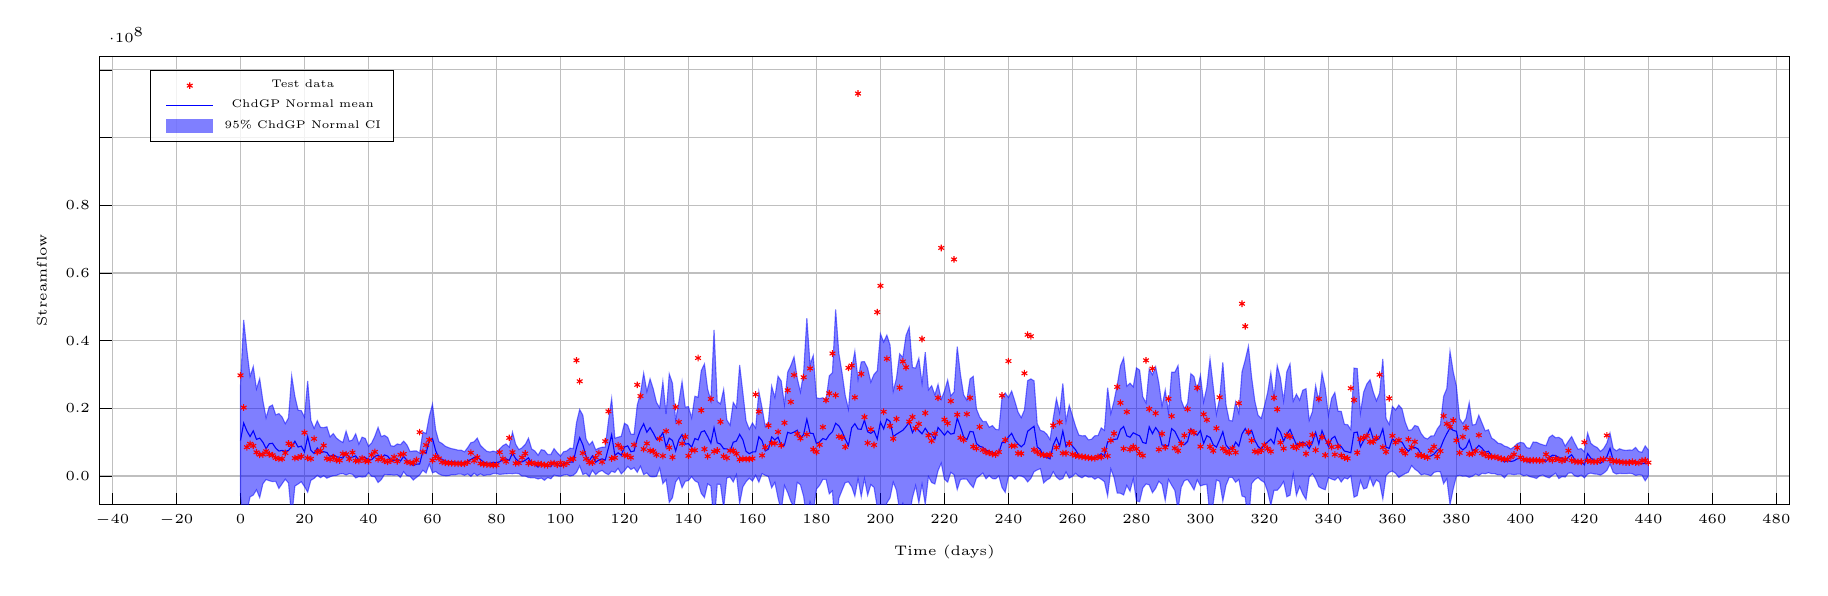
\begin{tikzpicture}

\definecolor{darkgray176}{RGB}{176,176,176}

\begin{axis}[
	font=\tiny,
	width=1.9\columnwidth,
	height=0.6\columnwidth,
	%axis background/.style={fill=background_color},
	%axis line style={white},
	tick align=inside,
	tick pos=left,
	%x grid style={white},
	%y grid style={white},
	xmajorgrids,
	ymajorgrids,
	ylabel={Streamflow},
	xlabel={Time (days)},
	% xmin=50, xmax=250,
	xtick style={color=black},
	% ymin=-10000000, % Adjusted to -0.1*10^8
	% ymax=80000000,  % Adjusted to 0.8*10^8
	ytick style={color=black},
	% ytick={-10000000,0,20000000,40000000,60000000,80000000}, % Updated ticks for new range
	yticklabels={
		\ensuremath{-}0.1,
		0.0,
		0.2,
		0.4,
		0.6,
		0.8
	},
	legend columns=1, 
	legend style={
		nodes={scale=0.8, transform shape},
		fill opacity=0.8,
		draw opacity=1,
		text opacity=1,
		at={(0.03,0.97)},
		anchor=north west,
		legend pos=north west,
		%draw=lightgray204,
		%fill=background_color
	}
	]
\path [draw=blue, fill=blue, opacity=0.5]
(axis cs:0,26692754.5928852)
--(axis cs:0,-5662112.16829846)
--(axis cs:1,-14885838.6300688)
--(axis cs:2,-10480413.3439129)
--(axis cs:3,-6144947.20226741)
--(axis cs:4,-5631711.97240175)
--(axis cs:5,-4076151.81922557)
--(axis cs:6,-6384399.82082017)
--(axis cs:7,-2284904.02443121)
--(axis cs:8,-1033228.31140354)
--(axis cs:9,-1388776.55744249)
--(axis cs:10,-1642560.23659469)
--(axis cs:11,-1563966.24132689)
--(axis cs:12,-3673361.28943867)
--(axis cs:13,-2304986.19720764)
--(axis cs:14,-920255.224949998)
--(axis cs:15,-2046851.10643412)
--(axis cs:16,-12263215.4955376)
--(axis cs:17,-2976309.67223035)
--(axis cs:18,-2372318.13296792)
--(axis cs:19,-1675058.46839529)
--(axis cs:20,-3120829.16986296)
--(axis cs:21,-4777032.00321441)
--(axis cs:22,-1271216.10426687)
--(axis cs:23,-706786.609418362)
--(axis cs:24,201284.869320879)
--(axis cs:25,-486375.217012184)
--(axis cs:26,80995.878741757)
--(axis cs:27,-634344.280625734)
--(axis cs:28,-231197.826207374)
--(axis cs:29,83663.0176645266)
--(axis cs:30,177972.900329513)
--(axis cs:31,602192.826995902)
--(axis cs:32,702820.665001671)
--(axis cs:33,308364.781817391)
--(axis cs:34,705559.192334972)
--(axis cs:35,497693.927724772)
--(axis cs:36,-549135.054610429)
--(axis cs:37,-180806.431148409)
--(axis cs:38,-294520.699901345)
--(axis cs:39,-238280.742364119)
--(axis cs:40,997441.042309313)
--(axis cs:41,-91257.9592871545)
--(axis cs:42,-249513.583464212)
--(axis cs:43,-1932447.16322529)
--(axis cs:44,-1071275.92459605)
--(axis cs:45,448875.798475024)
--(axis cs:46,365443.910239278)
--(axis cs:47,369018.770759872)
--(axis cs:48,259753.090835726)
--(axis cs:49,402732.561429888)
--(axis cs:50,-418646.716635125)
--(axis cs:51,1271253.45196416)
--(axis cs:52,99744.3910786193)
--(axis cs:53,-81147.3927691649)
--(axis cs:54,-1180876.16602249)
--(axis cs:55,-407843.00240046)
--(axis cs:56,323969.288286651)
--(axis cs:57,1722857.9891653)
--(axis cs:58,892225.773464995)
--(axis cs:59,3519659.97891121)
--(axis cs:60,936023.984034883)
--(axis cs:61,1326486.11914417)
--(axis cs:62,602319.776965963)
--(axis cs:63,211241.885283314)
--(axis cs:64,88218.886534906)
--(axis cs:65,100223.608247617)
--(axis cs:66,392908.265642733)
--(axis cs:67,332381.669652094)
--(axis cs:68,582928.939549233)
--(axis cs:69,570357.565526686)
--(axis cs:70,205194.545312348)
--(axis cs:71,626846.591473191)
--(axis cs:72,-105994.946168907)
--(axis cs:73,830750.300257031)
--(axis cs:74,108810.793527086)
--(axis cs:75,636037.002916725)
--(axis cs:76,141288.727907629)
--(axis cs:77,328087.217046179)
--(axis cs:78,353635.09462602)
--(axis cs:79,739356.586564623)
--(axis cs:80,754307.407849818)
--(axis cs:81,475495.461071091)
--(axis cs:82,586663.449626471)
--(axis cs:83,656218.15329726)
--(axis cs:84,725658.804714953)
--(axis cs:85,673438.927194097)
--(axis cs:86,812274.707727869)
--(axis cs:87,686287.927266717)
--(axis cs:88,-11952.4757210482)
--(axis cs:89,-21998.5915369214)
--(axis cs:90,-427685.331400337)
--(axis cs:91,-556609.642700274)
--(axis cs:92,-544707.352231399)
--(axis cs:93,-886577.444203313)
--(axis cs:94,-599474.703395616)
--(axis cs:95,-1249313.90455727)
--(axis cs:96,-437475.64195723)
--(axis cs:97,-821371.95643879)
--(axis cs:98,291815.930551053)
--(axis cs:99,41661.3037226521)
--(axis cs:100,-75801.7657932425)
--(axis cs:101,305175.935662654)
--(axis cs:102,429031.757162482)
--(axis cs:103,-23610.5425811913)
--(axis cs:104,225087.133469042)
--(axis cs:105,1036805.5214201)
--(axis cs:106,3005533.69530437)
--(axis cs:107,448974.469234617)
--(axis cs:108,800058.57436498)
--(axis cs:109,-146801.563199325)
--(axis cs:110,1691844.38460586)
--(axis cs:111,397026.609707654)
--(axis cs:112,1233208.25604864)
--(axis cs:113,1653158.52331748)
--(axis cs:114,878022.979690365)
--(axis cs:115,387496.428506384)
--(axis cs:116,1417445.22531536)
--(axis cs:117,1049541.28299098)
--(axis cs:118,2271996.25738952)
--(axis cs:119,634438.906453979)
--(axis cs:120,1563756.81339314)
--(axis cs:121,2836220.00158722)
--(axis cs:122,1930099.34317341)
--(axis cs:123,2427040.90715986)
--(axis cs:124,1101882.05718795)
--(axis cs:125,2907628.09056565)
--(axis cs:126,431714.79499449)
--(axis cs:127,917172.142446332)
--(axis cs:128,-156278.704373477)
--(axis cs:129,-262478.679903181)
--(axis cs:130,-115618.401567744)
--(axis cs:131,2336157.9092022)
--(axis cs:132,-2251166.16110842)
--(axis cs:133,-1051200.13374888)
--(axis cs:134,-7812163.46913287)
--(axis cs:135,-6405775.32168945)
--(axis cs:136,-1703389.8157927)
--(axis cs:137,-469596.714118529)
--(axis cs:138,-3475283.32360451)
--(axis cs:139,-1550885.21269034)
--(axis cs:140,-1340805.02508633)
--(axis cs:141,-175178.384136504)
--(axis cs:142,-1407907.1578605)
--(axis cs:143,-1928249.21052044)
--(axis cs:144,-5111490.57240144)
--(axis cs:145,-6360363.18005225)
--(axis cs:146,-2315570.52268239)
--(axis cs:147,-2943237.80081299)
--(axis cs:148,-14610596.9254716)
--(axis cs:149,-2409408.21804966)
--(axis cs:150,-2462930.85261496)
--(axis cs:151,-9485217.78983229)
--(axis cs:152,-553417.605709388)
--(axis cs:153,-289350.354811632)
--(axis cs:154,-1747601.59562802)
--(axis cs:155,406545.709124632)
--(axis cs:156,-8186548.62464621)
--(axis cs:157,-3207934.36816679)
--(axis cs:158,-1690356.37532246)
--(axis cs:159,-630765.546223613)
--(axis cs:160,-1472851.11515688)
--(axis cs:161,209893.924561661)
--(axis cs:162,-1817314.10644873)
--(axis cs:163,703635.882007815)
--(axis cs:164,219751.090127967)
--(axis cs:165,-179544.524431948)
--(axis cs:166,-3478073.14518974)
--(axis cs:167,-1850131.76971801)
--(axis cs:168,-6512649.0920999)
--(axis cs:169,-10331893.9346026)
--(axis cs:170,-2791622.88004317)
--(axis cs:171,-4863555.68943306)
--(axis cs:172,-7498511.8054854)
--(axis cs:173,-9244008.35104558)
--(axis cs:174,-1851251.13370107)
--(axis cs:175,-2588480.07310133)
--(axis cs:176,-6060407.37655238)
--(axis cs:177,-13086522.1530605)
--(axis cs:178,-7612585.37863388)
--(axis cs:179,-10507476.4666943)
--(axis cs:180,-3873949.22283278)
--(axis cs:181,-2719586.81527283)
--(axis cs:182,-995259.274400268)
--(axis cs:183,-1011754.90796614)
--(axis cs:184,-5249622.21526679)
--(axis cs:185,-4371040.06291306)
--(axis cs:186,-18071439.5966569)
--(axis cs:187,-6601638.64916942)
--(axis cs:188,-4212321.28319712)
--(axis cs:189,-1936052.26936105)
--(axis cs:190,-1742825.40120364)
--(axis cs:191,-3146025.95755043)
--(axis cs:192,-5952903.36406717)
--(axis cs:193,-774996.959777899)
--(axis cs:194,-6091250.67569053)
--(axis cs:195,-770697.809944917)
--(axis cs:196,-5664099.28148302)
--(axis cs:197,-2519876.04008893)
--(axis cs:198,-3374779.97759172)
--(axis cs:199,-9204444.73475063)
--(axis cs:200,-10187350.5312939)
--(axis cs:201,-11721736.7390221)
--(axis cs:202,-7953887.15431301)
--(axis cs:203,-6451569.44618112)
--(axis cs:204,-1774541.52391942)
--(axis cs:205,-4173475.89022581)
--(axis cs:206,-10215927.4940256)
--(axis cs:207,-8064826.83295927)
--(axis cs:208,-12366996.7983258)
--(axis cs:209,-12060058.5298647)
--(axis cs:210,-6400918.80866007)
--(axis cs:211,-2847387.45557456)
--(axis cs:212,-7942466.99748626)
--(axis cs:213,-2427072.99428016)
--(axis cs:214,-8384051.24377371)
--(axis cs:215,-201507.360982142)
--(axis cs:216,-1909727.07347262)
--(axis cs:217,-2360304.82041908)
--(axis cs:218,1597006.151159)
--(axis cs:219,3808269.72235203)
--(axis cs:220,-939090.000616295)
--(axis cs:221,-1798271.94003741)
--(axis cs:222,1078165.28206891)
--(axis cs:223,367922.207847724)
--(axis cs:224,-3974904.71463912)
--(axis cs:225,-1013958.84062228)
--(axis cs:226,-872730.598901672)
--(axis cs:227,-948946.265785402)
--(axis cs:228,-2318754.37625673)
--(axis cs:229,-3398474.01679925)
--(axis cs:230,-638463.835131403)
--(axis cs:231,94931.8434038777)
--(axis cs:232,872707.01182225)
--(axis cs:233,-816852.250407382)
--(axis cs:234,159058.382378913)
--(axis cs:235,-777120.392339205)
--(axis cs:236,-835154.871228354)
--(axis cs:237,41206.0579081876)
--(axis cs:238,-3382070.00034892)
--(axis cs:239,-4796917.11624279)
--(axis cs:240,-73874.7580162156)
--(axis cs:241,107372.640395695)
--(axis cs:242,-929403.791076755)
--(axis cs:243,34364.4527383354)
--(axis cs:244,16537.2821756881)
--(axis cs:245,-456565.607410483)
--(axis cs:246,-1726589.62141609)
--(axis cs:247,-752422.938115334)
--(axis cs:248,1275799.05799114)
--(axis cs:249,1806560.31068042)
--(axis cs:250,2173178.2374693)
--(axis cs:251,-2036668.57059763)
--(axis cs:252,-1171649.84813615)
--(axis cs:253,-633554.443237013)
--(axis cs:254,1287407.9406368)
--(axis cs:255,-301513.512815276)
--(axis cs:256,-1092640.90784783)
--(axis cs:257,-757729.803943601)
--(axis cs:258,1206707.53008867)
--(axis cs:259,-618113.306259416)
--(axis cs:260,-140124.731488582)
--(axis cs:261,790292.451437218)
--(axis cs:262,-67840.7520974549)
--(axis cs:263,-535850.131705164)
--(axis cs:264,154387.089837983)
--(axis cs:265,-346245.889678376)
--(axis cs:266,-245863.793879427)
--(axis cs:267,-941045.738588604)
--(axis cs:268,-369965.034065384)
--(axis cs:269,-958443.135020113)
--(axis cs:270,-1679549.35339229)
--(axis cs:271,-5867962.29384109)
--(axis cs:272,2097653.52289167)
--(axis cs:273,-454186.382988423)
--(axis cs:274,-5028436.72725076)
--(axis cs:275,-5087087.63017582)
--(axis cs:276,-5600322.65972684)
--(axis cs:277,-2792749.35545186)
--(axis cs:278,-4506238.22885343)
--(axis cs:279,-778794.682627253)
--(axis cs:280,-7342699.31501523)
--(axis cs:281,-7598540.64916123)
--(axis cs:282,-3544668.48966556)
--(axis cs:283,-2331439.29471632)
--(axis cs:284,-2604843.87728179)
--(axis cs:285,-4924125.09249656)
--(axis cs:286,-3657135.91349842)
--(axis cs:287,-1556644.81768519)
--(axis cs:288,-2444850.07710938)
--(axis cs:289,-7219556.54973427)
--(axis cs:290,-999561.48600206)
--(axis cs:291,-2695666.70408171)
--(axis cs:292,-4269225.00577515)
--(axis cs:293,-9997820.28552387)
--(axis cs:294,-3277783.0934585)
--(axis cs:295,-1347826.63765208)
--(axis cs:296,-1041049.79980692)
--(axis cs:297,-2436662.83371211)
--(axis cs:298,-4090170.85494504)
--(axis cs:299,-1106431.50527332)
--(axis cs:300,-2910123.6262331)
--(axis cs:301,-2602272.75237979)
--(axis cs:302,-2453532.96748069)
--(axis cs:303,-11799129.8317256)
--(axis cs:304,-8001098.24351062)
--(axis cs:305,-1170096.56764388)
--(axis cs:306,-1563738.50893784)
--(axis cs:307,-7444557.13922032)
--(axis cs:308,-2677008.60793237)
--(axis cs:309,-419954.289004729)
--(axis cs:310,-415829.696966474)
--(axis cs:311,-1852095.39620537)
--(axis cs:312,-992220.086432649)
--(axis cs:313,-5918696.39191244)
--(axis cs:314,-6249382.16555734)
--(axis cs:315,-13979031.6501071)
--(axis cs:316,-2249968.32392491)
--(axis cs:317,-1066510.49755923)
--(axis cs:318,-457500.612504641)
--(axis cs:319,-1302164.39262189)
--(axis cs:320,-1892937.65357995)
--(axis cs:321,-4554798.36445037)
--(axis cs:322,-8675760.95325467)
--(axis cs:323,-4213421.00218009)
--(axis cs:324,-4200095.23406326)
--(axis cs:325,-3141200.77886222)
--(axis cs:326,-1625952.86652775)
--(axis cs:327,-6131923.11536008)
--(axis cs:328,-5677424.70689616)
--(axis cs:329,692832.71665464)
--(axis cs:330,-5690820.89368555)
--(axis cs:331,-3076019.34026972)
--(axis cs:332,-5341600.41755037)
--(axis cs:333,-6921542.55610839)
--(axis cs:334,-228739.895264331)
--(axis cs:335,701091.61721709)
--(axis cs:336,-841532.072465995)
--(axis cs:337,-3150976.43331343)
--(axis cs:338,-3705060.58742797)
--(axis cs:339,-4037163.32870614)
--(axis cs:340,-445577.786538318)
--(axis cs:341,-895364.188055128)
--(axis cs:342,-1220510.40361609)
--(axis cs:343,-324415.590790428)
--(axis cs:344,-1758723.51428001)
--(axis cs:345,-529307.676761732)
--(axis cs:346,-872328.957707504)
--(axis cs:347,48832.5269203559)
--(axis cs:348,-6251075.57941063)
--(axis cs:349,-5781702.10739502)
--(axis cs:350,-1350586.56835958)
--(axis cs:351,-3821656.44164428)
--(axis cs:352,-3494200.00601863)
--(axis cs:353,-356408.612275111)
--(axis cs:354,-2984213.40654075)
--(axis cs:355,-1151553.35093127)
--(axis cs:356,-1863422.25575337)
--(axis cs:357,-6765570.14716807)
--(axis cs:358,76379.0629635789)
--(axis cs:359,1109552.60444308)
--(axis cs:360,1469495.96240128)
--(axis cs:361,794138.970168246)
--(axis cs:362,-433244.295208948)
--(axis cs:363,172415.357664444)
--(axis cs:364,709975.483785383)
--(axis cs:365,1137068.703185)
--(axis cs:366,3093258.18948311)
--(axis cs:367,2043644.46734392)
--(axis cs:368,1356774.63644818)
--(axis cs:369,329895.031462879)
--(axis cs:370,612963.668314484)
--(axis cs:371,405748.137823052)
--(axis cs:372,59376.5723565482)
--(axis cs:373,1063213.61946943)
--(axis cs:374,1323120.06711701)
--(axis cs:375,1243274.7460489)
--(axis cs:376,-2267041.94709228)
--(axis cs:377,-784422.706935771)
--(axis cs:378,-8494406.15618601)
--(axis cs:379,-3871500.4615975)
--(axis cs:380,-71020.2232376765)
--(axis cs:381,232474.368277323)
--(axis cs:382,-59280.8423611904)
--(axis cs:383,15871.9916116968)
--(axis cs:384,-390712.738760399)
--(axis cs:385,-63741.5923508769)
--(axis cs:386,597744.164385349)
--(axis cs:387,116658.784287859)
--(axis cs:388,808197.124374662)
--(axis cs:389,676889.482537997)
--(axis cs:390,977038.561996828)
--(axis cs:391,715121.290826351)
--(axis cs:392,694169.333122051)
--(axis cs:393,341318.044202879)
--(axis cs:394,333881.213432789)
--(axis cs:395,-529427.426474356)
--(axis cs:396,568506.349388899)
--(axis cs:397,561769.58322162)
--(axis cs:398,393186.206775138)
--(axis cs:399,562958.846551446)
--(axis cs:400,580659.292220047)
--(axis cs:401,75655.8098773556)
--(axis cs:402,329396.7893265)
--(axis cs:403,-211286.315811067)
--(axis cs:404,-390992.451131671)
--(axis cs:405,-724647.988174772)
--(axis cs:406,40423.5453529293)
--(axis cs:407,310100.025110401)
--(axis cs:408,-235778.579924852)
--(axis cs:409,-551407.809544849)
--(axis cs:410,192660.669163283)
--(axis cs:411,839621.952383627)
--(axis cs:412,-739485.225433839)
--(axis cs:413,-186231.447533542)
--(axis cs:414,-304272.559390296)
--(axis cs:415,858775.59350675)
--(axis cs:416,933297.261301594)
--(axis cs:417,51340.7588700298)
--(axis cs:418,-200106.807903183)
--(axis cs:419,274609.99924298)
--(axis cs:420,-544019.416443991)
--(axis cs:421,566641.408124957)
--(axis cs:422,871718.765861371)
--(axis cs:423,620938.67777241)
--(axis cs:424,538398.553589696)
--(axis cs:425,260276.711738802)
--(axis cs:426,808843.342826717)
--(axis cs:427,1655700.46623607)
--(axis cs:428,3548522.14487459)
--(axis cs:429,1092459.82283566)
--(axis cs:430,581104.808641864)
--(axis cs:431,778459.050967624)
--(axis cs:432,711717.522830605)
--(axis cs:433,693817.087485776)
--(axis cs:434,817924.354349435)
--(axis cs:435,690770.11117014)
--(axis cs:436,179593.293798318)
--(axis cs:437,357384.82904783)
--(axis cs:438,265905.112572647)
--(axis cs:439,-1404875.50757486)
--(axis cs:440,37635.5179055259)
--(axis cs:440,7682915.94843399)
--(axis cs:440,7682915.94843399)
--(axis cs:439,8890410.34444551)
--(axis cs:438,7017913.8094197)
--(axis cs:437,7222970.30336319)
--(axis cs:436,8449602.16572868)
--(axis cs:435,7650862.41315396)
--(axis cs:434,7688786.72060122)
--(axis cs:433,7574940.75478851)
--(axis cs:432,7701851.00434637)
--(axis cs:431,8054936.28413256)
--(axis cs:430,7445707.49392711)
--(axis cs:429,8140287.54690779)
--(axis cs:428,12733261.4700819)
--(axis cs:427,9708676.81889813)
--(axis cs:426,8084822.51145728)
--(axis cs:425,7261488.68969588)
--(axis cs:424,8439928.67348011)
--(axis cs:423,8877186.49542934)
--(axis cs:422,9689124.48728516)
--(axis cs:421,12715662.6461316)
--(axis cs:420,7194448.7583119)
--(axis cs:419,8104031.41792603)
--(axis cs:418,7917386.23888413)
--(axis cs:417,9710441.41623257)
--(axis cs:416,11641921.3877141)
--(axis cs:415,10307318.9793235)
--(axis cs:414,8820732.96238766)
--(axis cs:413,10814906.8334449)
--(axis cs:412,11436059.1319427)
--(axis cs:411,11306363.155197)
--(axis cs:410,12089579.567352)
--(axis cs:409,11404952.385801)
--(axis cs:408,8959134.96276782)
--(axis cs:407,9216107.87432199)
--(axis cs:406,9542165.45034777)
--(axis cs:405,9987838.82813487)
--(axis cs:404,10042469.625733)
--(axis cs:403,8190648.40573185)
--(axis cs:402,8378456.75504256)
--(axis cs:401,9734331.66073321)
--(axis cs:400,9949662.43174207)
--(axis cs:399,9576611.74517198)
--(axis cs:398,8607140.79606134)
--(axis cs:397,7977983.35222325)
--(axis cs:396,8568670.03200991)
--(axis cs:395,8839119.93608782)
--(axis cs:394,9518310.23409956)
--(axis cs:393,9690454.55214396)
--(axis cs:392,10611751.5368361)
--(axis cs:391,11226415.9214885)
--(axis cs:390,13680468.18839)
--(axis cs:389,13335791.3597224)
--(axis cs:388,15658598.0359112)
--(axis cs:387,17969409.3378887)
--(axis cs:386,15239519.8575613)
--(axis cs:385,15069461.2345467)
--(axis cs:384,21703888.0612028)
--(axis cs:383,16978811.3375669)
--(axis cs:382,15504389.9301882)
--(axis cs:381,16911630.1877589)
--(axis cs:380,26522775.8717864)
--(axis cs:379,30834792.4639656)
--(axis cs:378,36904216.4782803)
--(axis cs:377,25853400.0540226)
--(axis cs:376,23535085.7144685)
--(axis cs:375,15190269.6336732)
--(axis cs:374,13883235.6986957)
--(axis cs:373,11888931.6915364)
--(axis cs:372,11817789.0425268)
--(axis cs:371,10947656.6821462)
--(axis cs:370,11321414.7004022)
--(axis cs:369,12521685.5694727)
--(axis cs:368,14618816.2661299)
--(axis cs:367,14939196.2807332)
--(axis cs:366,13653427.6360504)
--(axis cs:365,13522274.9716967)
--(axis cs:364,15924391.2912797)
--(axis cs:363,19838449.1672408)
--(axis cs:362,20956202.4703062)
--(axis cs:361,19488981.8618521)
--(axis cs:360,20574654.2515506)
--(axis cs:359,15244187.6313953)
--(axis cs:358,17003996.1110573)
--(axis cs:357,34638973.9547306)
--(axis cs:356,24506991.7725019)
--(axis cs:355,22205369.838325)
--(axis cs:354,24865576.2985659)
--(axis cs:353,28448276.0125585)
--(axis cs:352,27180570.805471)
--(axis cs:351,24741444.5629527)
--(axis cs:350,18633381.224081)
--(axis cs:349,31749257.8658058)
--(axis cs:348,31887359.7639122)
--(axis cs:347,13698103.9192623)
--(axis cs:346,15188298.1061937)
--(axis cs:345,15251714.9156512)
--(axis cs:344,19109165.7540476)
--(axis cs:343,19163077.7593976)
--(axis cs:342,24666403.7052464)
--(axis cs:341,22970505.4236649)
--(axis cs:340,17968832.4001072)
--(axis cs:339,25952979.3634421)
--(axis cs:338,30504077.3976327)
--(axis cs:337,22075788.0026611)
--(axis cs:336,26706180.8077169)
--(axis cs:335,19030596.4565807)
--(axis cs:334,16427440.2183058)
--(axis cs:333,25786947.5682956)
--(axis cs:332,25360392.8736789)
--(axis cs:331,22397780.3874725)
--(axis cs:330,24181183.4721)
--(axis cs:329,22079372.9269043)
--(axis cs:328,33141304.2538355)
--(axis cs:327,30824730.305841)
--(axis cs:326,22190606.2239408)
--(axis cs:325,28983242.2431803)
--(axis cs:324,32631762.0394669)
--(axis cs:323,23273412.0135501)
--(axis cs:322,30482210.2658169)
--(axis cs:321,24673360.2442917)
--(axis cs:320,20634191.1404051)
--(axis cs:319,17052153.6701936)
--(axis cs:318,18014082.0272252)
--(axis cs:317,22163274.9914902)
--(axis cs:316,29198370.4767197)
--(axis cs:315,38347609.7288174)
--(axis cs:314,34281350.8766412)
--(axis cs:313,30787575.4119385)
--(axis cs:312,18599537.3871621)
--(axis cs:311,21853022.9065278)
--(axis cs:310,16264117.4020845)
--(axis cs:309,16422780.4795096)
--(axis cs:308,21022830.0311427)
--(axis cs:307,33598189.5385573)
--(axis cs:306,22940147.497153)
--(axis cs:305,18249932.1896099)
--(axis cs:304,26483265.44846)
--(axis cs:303,34618946.6603875)
--(axis cs:302,26236994.9626558)
--(axis cs:301,21860681.6260315)
--(axis cs:300,29769667.3587872)
--(axis cs:299,25264192.7913433)
--(axis cs:298,29365023.2774201)
--(axis cs:297,30248974.6891761)
--(axis cs:296,21539572.2456523)
--(axis cs:295,19906102.8518964)
--(axis cs:294,22382163.8879393)
--(axis cs:293,32634078.6011208)
--(axis cs:292,30642972.5815024)
--(axis cs:291,30695516.6194301)
--(axis cs:290,18791991.2016789)
--(axis cs:289,25427241.1330181)
--(axis cs:288,20672311.4695069)
--(axis cs:287,27508607.2452503)
--(axis cs:286,32297139.4168471)
--(axis cs:285,29958435.1732761)
--(axis cs:284,31638869.1799247)
--(axis cs:283,21572632.3015058)
--(axis cs:282,23368294.9610463)
--(axis cs:281,31301565.6862032)
--(axis cs:280,31952221.4586313)
--(axis cs:279,26338113.3226909)
--(axis cs:278,27442330.5791846)
--(axis cs:277,26532959.2710052)
--(axis cs:276,34893398.1324818)
--(axis cs:275,32547554.8951709)
--(axis cs:274,26894590.625196)
--(axis cs:273,22119913.2851298)
--(axis cs:272,18464210.9581135)
--(axis cs:271,26084648.3174954)
--(axis cs:270,13489379.1946311)
--(axis cs:269,14214902.5548892)
--(axis cs:268,11959708.2146283)
--(axis cs:267,11882648.7817011)
--(axis cs:266,10885203.6002613)
--(axis cs:265,10686183.4185227)
--(axis cs:264,11912736.9968734)
--(axis cs:263,11873603.3331366)
--(axis cs:262,12103947.4820879)
--(axis cs:261,14634921.809776)
--(axis cs:260,17784466.3316464)
--(axis cs:259,20941269.5974438)
--(axis cs:258,16119061.3078717)
--(axis cs:257,27338785.051275)
--(axis cs:256,18638733.4295653)
--(axis cs:255,22814426.9595517)
--(axis cs:254,17038142.7748706)
--(axis cs:253,10746677.6031437)
--(axis cs:252,12327553.6460726)
--(axis cs:251,13186443.0150957)
--(axis cs:250,13472754.6548412)
--(axis cs:249,15429764.9625762)
--(axis cs:248,28126388.326336)
--(axis cs:247,28701081.8738068)
--(axis cs:246,28173086.9495867)
--(axis cs:245,19495055.171388)
--(axis cs:244,17245810.2249987)
--(axis cs:243,18877404.1974449)
--(axis cs:242,22135696.6765319)
--(axis cs:241,25112222.6945297)
--(axis cs:240,23196771.7016478)
--(axis cs:239,24544706.2903514)
--(axis cs:238,23198451.2746266)
--(axis cs:237,13667884.0209516)
--(axis cs:236,13779401.1161385)
--(axis cs:235,14906864.4413163)
--(axis cs:234,14389058.3413724)
--(axis cs:233,16108015.5726415)
--(axis cs:232,16094134.7068899)
--(axis cs:231,17471910.5661004)
--(axis cs:230,19812178.3329886)
--(axis cs:229,29438992.1424722)
--(axis cs:228,28686206.064409)
--(axis cs:227,22397602.6768772)
--(axis cs:226,24027545.420475)
--(axis cs:225,30053280.1507405)
--(axis cs:224,38226428.7886272)
--(axis cs:223,24835643.5398785)
--(axis cs:222,23684378.617741)
--(axis cs:221,28359659.3648896)
--(axis cs:220,25057861.9693991)
--(axis cs:219,22676002.455582)
--(axis cs:218,27073829.6155425)
--(axis cs:217,24005071.4683439)
--(axis cs:216,26677553.9134079)
--(axis cs:215,25451331.6738572)
--(axis cs:214,36601617.6597733)
--(axis cs:213,27391250.2324377)
--(axis cs:212,34786414.1134476)
--(axis cs:211,31901756.5449556)
--(axis cs:210,32062820.9653424)
--(axis cs:209,43935429.9292967)
--(axis cs:208,41552044.0628707)
--(axis cs:207,35109134.7422252)
--(axis cs:206,36091486.468827)
--(axis cs:205,28870848.3671178)
--(axis cs:204,25100788.8958717)
--(axis cs:203,38701656.0940791)
--(axis cs:202,41631727.7467995)
--(axis cs:201,39599101.1313364)
--(axis cs:200,42043771.6123293)
--(axis cs:199,31072702.1236248)
--(axis cs:198,30059480.5225438)
--(axis cs:197,27746111.8460251)
--(axis cs:196,31837123.8493243)
--(axis cs:195,33807970.6789439)
--(axis cs:194,33730323.1408484)
--(axis cs:193,28500606.0403548)
--(axis cs:192,36862310.6558947)
--(axis cs:191,31607270.2875)
--(axis cs:190,19777032.4173507)
--(axis cs:189,23784550.8044658)
--(axis cs:188,30511507.1236403)
--(axis cs:187,36235265.1102293)
--(axis cs:186,49225728.7151861)
--(axis cs:185,30541825.6519995)
--(axis cs:184,29582231.7283365)
--(axis cs:183,22470724.1745541)
--(axis cs:182,23125054.6420772)
--(axis cs:181,22888242.8728094)
--(axis cs:180,23124581.9546329)
--(axis cs:179,35597000.1699989)
--(axis cs:178,32947966.5438801)
--(axis cs:177,46656121.1845531)
--(axis cs:176,30703980.4453008)
--(axis cs:175,24825131.7057315)
--(axis cs:174,28919087.4355058)
--(axis cs:173,35234384.7081276)
--(axis cs:172,32673356.2563247)
--(axis cs:171,30665944.9405378)
--(axis cs:170,21100429.5869902)
--(axis cs:169,28055735.6998245)
--(axis cs:168,29491718.171196)
--(axis cs:167,23227856.3721087)
--(axis cs:166,26587312.0369671)
--(axis cs:165,16101991.9532122)
--(axis cs:164,14590080.3682061)
--(axis cs:163,20207807.4596162)
--(axis cs:162,24996863.3190708)
--(axis cs:161,14146914.9884588)
--(axis cs:160,15663818.5737373)
--(axis cs:159,13818412.5571923)
--(axis cs:158,16291759.7155398)
--(axis cs:157,24630551.577171)
--(axis cs:156,32796842.6798978)
--(axis cs:155,20242295.5397204)
--(axis cs:154,21742006.5291947)
--(axis cs:153,15010806.1358018)
--(axis cs:152,16593668.767773)
--(axis cs:151,25612006.671512)
--(axis cs:150,21323162.7365713)
--(axis cs:149,22013738.9940483)
--(axis cs:148,43175738.3648692)
--(axis cs:147,22348663.5540476)
--(axis cs:146,25667401.7476975)
--(axis cs:145,33119733.7504703)
--(axis cs:144,31166013.1292091)
--(axis cs:143,23264687.7604028)
--(axis cs:142,23568553.2545137)
--(axis cs:141,17175786.7656553)
--(axis cs:140,20493081.6707247)
--(axis cs:139,20373416.3661325)
--(axis cs:138,27943024.4349553)
--(axis cs:137,21921060.0383165)
--(axis cs:136,16548609.9672775)
--(axis cs:135,27416370.222886)
--(axis cs:134,30173355.4561506)
--(axis cs:133,18313722.5444946)
--(axis cs:132,27913557.2954709)
--(axis cs:131,20149535.7986401)
--(axis cs:130,21766552.247302)
--(axis cs:129,25717314.331037)
--(axis cs:128,28731099.7020139)
--(axis cs:127,24961417.6357092)
--(axis cs:126,30416080.6056253)
--(axis cs:125,24400883.7665611)
--(axis cs:124,20976345.082501)
--(axis cs:123,12335673.989535)
--(axis cs:122,12397262.0118157)
--(axis cs:121,14986121.8088276)
--(axis cs:120,15590062.8036895)
--(axis cs:119,11727929.0676087)
--(axis cs:118,11469461.0549833)
--(axis cs:117,11152344.3869495)
--(axis cs:116,22910985.9303087)
--(axis cs:115,16347693.8686677)
--(axis cs:114,8537618.39156092)
--(axis cs:113,8502327.60159439)
--(axis cs:112,8229748.66519473)
--(axis cs:111,7749284.11900719)
--(axis cs:110,10211264.3868914)
--(axis cs:109,9204155.56364275)
--(axis cs:108,10899677.0360872)
--(axis cs:107,17940510.451671)
--(axis cs:106,19662722.5558849)
--(axis cs:105,15730915.8694964)
--(axis cs:104,8089998.95190402)
--(axis cs:103,8225097.27253151)
--(axis cs:102,7407034.57322459)
--(axis cs:101,7176882.11675728)
--(axis cs:100,5917363.12101229)
--(axis cs:99,6884259.69115505)
--(axis cs:98,8102629.02960125)
--(axis cs:97,6345112.9918143)
--(axis cs:96,6346732.40676958)
--(axis cs:95,7569632.26375539)
--(axis cs:94,7764156.05043051)
--(axis cs:93,6137533.45443822)
--(axis cs:92,7392891.6079323)
--(axis cs:91,7990515.56437712)
--(axis cs:90,11181660.2228351)
--(axis cs:89,9328665.75068232)
--(axis cs:88,8364710.82606661)
--(axis cs:87,7801421.02183045)
--(axis cs:86,9407571.43031752)
--(axis cs:85,12975705.2287843)
--(axis cs:84,8532550.85651354)
--(axis cs:83,9488032.6781169)
--(axis cs:82,8970319.02359893)
--(axis cs:81,7975735.06849188)
--(axis cs:80,7053576.6615939)
--(axis cs:79,7367820.84915374)
--(axis cs:78,7094447.77006984)
--(axis cs:77,7294383.79326362)
--(axis cs:76,8095847.20136094)
--(axis cs:75,9029142.82334839)
--(axis cs:74,11211780.5796897)
--(axis cs:73,10101324.6501443)
--(axis cs:72,9844197.56991893)
--(axis cs:71,8369098.5406026)
--(axis cs:70,7141374.39345284)
--(axis cs:69,7644044.46839755)
--(axis cs:68,7638988.54894682)
--(axis cs:67,7887369.46374802)
--(axis cs:66,8084045.19422925)
--(axis cs:65,8403148.95247725)
--(axis cs:64,8799924.33198582)
--(axis cs:63,9613011.95371111)
--(axis cs:62,10146578.089845)
--(axis cs:61,13598452.8042418)
--(axis cs:60,21251826.4641403)
--(axis cs:59,17586351.8223433)
--(axis cs:58,12514436.5307578)
--(axis cs:57,13033850.3594969)
--(axis cs:56,6805385.5090193)
--(axis cs:55,7400257.88449772)
--(axis cs:54,7391626.83332495)
--(axis cs:53,7244062.82339362)
--(axis cs:52,9209718.97936578)
--(axis cs:51,10311208.5385612)
--(axis cs:50,9267258.5773678)
--(axis cs:49,9473477.95002471)
--(axis cs:48,8790796.46788294)
--(axis cs:47,8936454.35014224)
--(axis cs:46,11396064.9291737)
--(axis cs:45,12018006.9447923)
--(axis cs:44,11652328.6691202)
--(axis cs:43,14363641.7452561)
--(axis cs:42,11774828.613567)
--(axis cs:41,9779658.87901797)
--(axis cs:40,8787616.1038871)
--(axis cs:39,11114802.9280381)
--(axis cs:38,11488166.5519333)
--(axis cs:37,9423703.04417897)
--(axis cs:36,12456509.7702157)
--(axis cs:35,10660939.2322181)
--(axis cs:34,10285289.8405068)
--(axis cs:33,13253432.6742137)
--(axis cs:32,9900706.41339085)
--(axis cs:31,10468604.9699162)
--(axis cs:30,11192882.3913839)
--(axis cs:29,12535790.9582439)
--(axis cs:28,11555737.7581291)
--(axis cs:27,14542429.9001067)
--(axis cs:26,14294437.0099934)
--(axis cs:25,14380241.988514)
--(axis cs:24,16324478.1853898)
--(axis cs:23,14057929.3260777)
--(axis cs:22,16459842.0177998)
--(axis cs:21,28080903.737946)
--(axis cs:20,17396361.2015598)
--(axis cs:19,19336372.0614135)
--(axis cs:18,19481876.867474)
--(axis cs:17,23546578.491129)
--(axis cs:16,29633625.2683251)
--(axis cs:15,17153728.7752596)
--(axis cs:14,15464852.0924091)
--(axis cs:13,17416247.7728366)
--(axis cs:12,18441000.246992)
--(axis cs:11,18072149.5237422)
--(axis cs:10,20983937.7820313)
--(axis cs:9,20489550.1108952)
--(axis cs:8,17184974.5875203)
--(axis cs:7,22273180.8378057)
--(axis cs:6,28774387.0844977)
--(axis cs:5,25727214.8089712)
--(axis cs:4,32327618.2591431)
--(axis cs:3,29471583.6222282)
--(axis cs:2,37173036.7583126)
--(axis cs:1,46144719.5964781)
--(axis cs:0,26692754.5928852)
--cycle;

\addplot [only marks, red, mark=asterisk, mark size=1.2]
table {%
0 29755500
1 20228000
2 8513700
3 9502900
4 8909200
5 7004800
6 6305500
7 6348400
8 7321100
9 6421300
10 6164800
11 5360500
12 5074700
13 5074700
14 6804600
15 9612000
16 9154100
17 5291400
18 5456200
19 5819200
20 12820200
21 5305900
22 5067000
23 11001200
24 7051300
25 7450000
26 9014400
27 5198200
28 4916300
29 5534800
30 4719000
31 4596600
32 6568000
33 6431200
34 5034500
35 6933000
36 4533400
37 4446000
38 5301600
39 4517400
40 4370200
41 6208600
42 7137600
43 4905200
44 5415600
45 4461400
46 4170200
47 4549000
48 5623500
49 4354800
50 6282500
51 6528100
52 4165200
53 3940800
54 3894500
55 4728400
56 12964300
57 7101500
58 9158000
59 10692100
60 4636300
61 5787600
62 5199600
63 4093600
64 3925700
65 3818200
66 3756600
67 3702000
68 3632400
69 3676500
70 3599700
71 4028000
72 6895400
73 4511900
74 5519200
75 3725000
76 3495900
77 3418000
78 3308300
79 3208300
80 3241700
81 7029700
82 5106300
83 4259800
84 11266900
85 7029700
86 3754100
87 3833100
88 5472000
89 6634600
90 3756400
91 3932500
92 3587100
93 3677400
94 3490000
95 3271000
96 3169400
97 3754100
98 3754100
99 3289100
100 3907600
101 3268800
102 3747400
103 4939300
104 5061200
105 34188900
106 27994500
107 6776800
108 5061200
109 4065600
110 3948300
111 5492400
112 6815200
113 4162700
114 10287200
115 19116000
116 5162800
117 5390800
118 9111000
119 8332200
120 6176400
121 6007000
122 5449500
123 9217100
124 26947100
125 23633100
126 7943900
127 9619000
128 7515000
129 7323100
130 6271200
131 10975700
132 5934800
133 13255700
134 8424800
135 5537500
136 20382400
137 15957800
138 9571500
139 11587400
140 5961900
141 7573700
142 7627900
143 34868400
144 19389200
145 7959700
146 5842300
147 22768500
148 7232800
149 7546600
150 16027800
151 5833200
152 5336600
153 7476600
154 7512800
155 6573700
156 4891900
157 5083800
158 4998000
159 5007000
160 5165000
161 24100400
162 19050500
163 6097300
164 8512800
165 14923900
166 9695700
167 9673100
168 13014100
169 9045600
170 15720800
171 25333000
172 21901700
173 29845600
174 12422700
175 11126900
176 29179700
177 12285000
178 31793800
179 7835600
180 7106400
181 9212600
182 14449900
183 22425400
184 24443600
185 36209300
186 23874700
187 11655200
188 11354900
189 8605400
190 31960800
191 32662900
192 23240300
193 113027800
194 30163900
195 17425200
196 9767900
197 13793000
198 9176500
199 48431100
200 56194500
201 19000900
202 34642700
203 14820100
204 11009500
205 16849500
206 26134400
207 33843500
208 32130100
209 16087400
210 17438700
211 14080400
212 15384500
213 40475900
214 18610300
215 11987000
216 10382000
217 12513000
218 23102600
219 67402600
220 16682500
221 15589900
222 22150000
223 64014200
224 18127200
225 11294600
226 10635400
227 18295300
228 23097100
229 8678100
230 8156300
231 14513900
232 7707800
233 7069100
234 6833500
235 6511900
236 6344300
237 7089500
238 23791600
239 10674900
240 33965900
241 8903700
242 8915100
243 6704400
244 6631900
245 30353300
246 41741700
247 41295500
248 7716900
249 7114400
250 6434900
251 6253700
252 6063400
253 6285400
254 14942200
255 8441700
256 15918400
257 6738400
258 6738400
259 9590000
260 6439400
261 6058900
262 5855000
263 5691900
264 5549300
265 5404300
266 5284200
267 5207200
268 5669300
269 5574200
270 7710100
271 5907100
272 10505100
273 12550400
274 26328400
275 21633000
276 8083800
277 18942200
278 7873100
279 8684000
280 8011300
281 6641000
282 6031700
283 34190200
284 19821000
285 31746200
286 18552600
287 7839200
288 12471100
289 8468800
290 22822100
291 17691900
292 8228700
293 7429200
294 9578700
295 11988600
296 19771200
297 13257000
298 12799500
299 26049800
300 8720300
301 18244600
302 16595700
303 8638700
304 7465400
305 14095100
306 23268300
307 8117800
308 7275200
309 6851600
310 8199300
311 6978500
312 21503900
313 50912700
314 44235500
315 13080400
316 10482400
317 7288800
318 7094000
319 7544700
320 9150600
321 8079300
322 7254800
323 23109800
324 19705500
325 9900300
326 8115500
327 12027200
328 11605900
329 8681700
330 8289900
331 9282000
332 9334100
333 6591200
334 9687400
335 12131300
336 7669300
337 22799500
338 11479000
339 6181200
340 10036200
341 8566200
342 6348800
343 8690800
344 6029400
345 5472200
346 5182300
347 25941000
348 22471100
349 6924100
350 10926400
351 11340900
352 11861800
353 10104200
354 10158500
355 11315900
356 29934200
357 8493800
358 7152900
359 22946700
360 11884500
361 9943400
362 10604700
363 7551500
364 6679500
365 10824400
366 8539100
367 10095100
368 6169900
369 6054300
370 5782500
371 5451900
372 7485800
373 8675000
374 5766700
375 7368000
376 17732700
377 15408800
378 14600200
379 16423500
380 10514100
381 6847100
382 11556000
383 14274000
384 6534500
385 6545900
386 7393000
387 12083800
388 6767800
389 6280800
390 5789300
391 5710100
392 5662500
393 5395200
394 5094000
395 4915100
396 4906000
397 5605900
398 6364700
399 8364600
400 5513000
401 4910500
402 4724800
403 4636500
404 4645500
405 4625100
406 4575300
407 4518700
408 6396400
409 5037400
410 4656800
411 5141600
412 4847100
413 4466600
414 4971700
415 7485800
416 4645500
417 4308000
418 4185700
419 4208400
420 9963700
421 4541300
422 4280900
423 4249100
424 4262700
425 4792700
426 4940000
427 12004500
428 4865200
429 4317100
430 4405400
431 4178900
432 4077000
433 3970500
434 3990900
435 4215200
436 3959200
437 3877700
438 4516400
439 4643300
440 3959200
};
\addplot [blue]
table {%
0 10515321.2122933
1 15629440.4832046
2 13346311.7071999
3 11663318.2099804
4 13347953.1433707
5 10825531.4948728
6 11194993.6318388
7 9994138.40668725
8 8075873.13805837
9 9550386.77672637
10 9670688.7727183
11 8254091.64120766
12 7383819.47877664
13 7555630.7878145
14 7272298.43372957
15 7553438.83441274
16 8685204.88639375
17 10285134.4094493
18 8554779.36725305
19 8830656.7965091
20 7137766.01584843
21 11651935.8673658
22 7594312.95676647
23 6675571.35832966
24 8262881.52735532
25 6946933.38575091
26 7187716.4443676
27 6954042.80974048
28 5662269.96596085
29 6309726.98795422
30 5685427.64585671
31 5535398.89845605
32 5301763.53919626
33 6780898.72801555
34 5495424.51642087
35 5579316.57997142
36 5953687.35780265
37 4621448.30651528
38 5596822.92601597
39 5438261.09283698
40 4892528.57309821
41 4844200.45986541
42 5762657.51505138
43 6215597.29101538
44 5290526.37226208
45 6233441.37163364
46 5880754.41970649
47 4652736.56045106
48 4525274.77935933
49 4938105.2557273
50 4424305.93036634
51 5791230.99526266
52 4654731.6852222
53 3581457.71531223
54 3105375.33365123
55 3496207.44104863
56 3564677.39865297
57 7378354.1743311
58 6703331.15211141
59 10553005.9006272
60 11093925.2240876
61 7462469.46169299
62 5374448.93340546
63 4912126.91949721
64 4444071.60926036
65 4251686.28036243
66 4238476.72993599
67 4109875.56670006
68 4110958.74424803
69 4107201.01696212
70 3673284.46938259
71 4497972.56603789
72 4869101.31187501
73 5466037.47520065
74 5660295.6866084
75 4832589.91313256
76 4118567.96463428
77 3811235.5051549
78 3724041.43234793
79 4053588.71785918
80 3903942.03472186
81 4225615.26478149
82 4778491.2366127
83 5072125.41570708
84 4629104.83061424
85 6824572.07798918
86 5109923.0690227
87 4243854.47454858
88 4176379.17517278
89 4653333.5795727
90 5376987.44571736
91 3716952.96083842
92 3424092.12785045
93 2625478.00511745
94 3582340.67351745
95 3160159.17959906
96 2954628.38240618
97 2761870.51768776
98 4197222.48007615
99 3462960.49743885
100 2920780.67760952
101 3741029.02620996
102 3918033.16519353
103 4100743.36497516
104 4157543.04268653
105 8383860.69545823
106 11334128.1255946
107 9194742.46045283
108 5849867.8052261
109 4528677.00022171
110 5951554.38574864
111 4073155.36435742
112 4731478.46062168
113 5077743.06245593
114 4707820.68562564
115 8367595.14858704
116 12164215.577812
117 6100942.83497024
118 6870728.65618642
119 6181183.98703135
120 8576909.80854133
121 8911170.90520741
122 7163680.67749456
123 7381357.44834743
124 11039113.5698445
125 13654255.9285634
126 15423897.7003099
127 12939294.8890778
128 14287410.4988202
129 12727417.8255669
130 10825466.9228672
131 11242846.8539212
132 12831195.5671813
133 8631261.20537287
134 11180595.9935089
135 10505297.4505983
136 7422610.07574242
137 10725731.662099
138 12233870.5556754
139 9411265.57672107
140 9576138.32281919
141 8500304.1907594
142 11080323.0483266
143 10668219.2749412
144 13027261.2784038
145 13379685.285209
146 11675915.6125076
147 9702712.87661731
148 14282570.7196988
149 9802165.38799934
150 9430115.94197817
151 8063394.44083984
152 8020125.58103179
153 7360727.89049507
154 9997202.46678334
155 10324420.6244225
156 12305147.0276258
157 10711308.6045021
158 7300701.67010866
159 6593823.50548436
160 7095483.72929021
161 7178404.45651024
162 11589774.606311
163 10455721.670812
164 7404915.72916706
165 7961223.71439015
166 11554619.4458887
167 10688862.3011953
168 11489534.539548
169 8861920.88261094
170 9154403.35347351
171 12901194.6255523
172 12587422.2254197
173 12995188.178541
174 13533918.1509024
175 11118325.8163151
176 12321786.5343742
177 16784799.5157463
178 12667690.5826231
179 12544761.8516523
180 9625316.36590004
181 10084328.0287683
182 11064897.6838384
183 10729484.633294
184 12166304.7565349
185 13085392.7945432
186 15577144.5592646
187 14816813.2305299
188 13149592.9202216
189 10924249.2675524
190 9017103.50807354
191 14230622.1649748
192 15454703.6459138
193 13862804.5402884
194 13819536.232579
195 16518636.4344995
196 13086512.2839206
197 12613117.9029681
198 13342350.2724761
199 10934128.6944371
200 15928210.5405177
201 13938682.1961572
202 16838920.2962433
203 16125043.323949
204 11663123.6859762
205 12348686.238446
206 12937779.4874007
207 13522153.9546329
208 14592523.6322724
209 15937685.699716
210 12830951.0783412
211 14527184.5446905
212 13421973.5579807
213 12482088.6190788
214 14108783.2079998
215 12624912.1564375
216 12383913.4199677
217 10822383.3239624
218 14335417.8833508
219 13242136.088967
220 12059385.9843914
221 13280693.7124261
222 12381271.9499049
223 12601782.8738631
224 17125762.036994
225 14519660.6550591
226 11577407.4107866
227 10724328.2055459
228 13183725.8440761
229 13020259.0628365
230 9586857.24892861
231 8783421.20475216
232 8483420.85935609
233 7645581.66111708
234 7274058.36187565
235 7064872.02448854
236 6472123.12245508
237 6854545.03942988
238 9908190.63713884
239 9873894.5870543
240 11561448.4718158
241 12609797.6674627
242 10603146.4427276
243 9455884.32509162
244 8631173.75358721
245 9519244.78198875
246 13223248.6640853
247 13974329.4678458
248 14701093.6921635
249 8618162.63662831
250 7822966.44615523
251 5574887.22224903
252 5577951.89896821
253 5056561.57995333
254 9162775.35775372
255 11256456.7233682
256 8773046.26085872
257 13290527.6236657
258 8662884.41898018
259 10161578.1455922
260 8822170.8000789
261 7712607.13060659
262 6018053.3649952
263 5668876.60071574
264 6033562.04335567
265 5169968.76442214
266 5319669.90319096
267 5470801.52155626
268 5794871.59028147
269 6628229.70993455
270 5904914.92061938
271 10108343.0118271
272 10280932.2405026
273 10832863.4510707
274 10933076.9489726
275 13730233.6324975
276 14646537.7363775
277 11870104.9577767
278 11468046.1751656
279 12779659.3200318
280 12304761.071808
281 11851512.518521
282 9911813.23569036
283 9620596.50339475
284 14517012.6513215
285 12517155.0403898
286 14320001.7516743
287 12975981.2137826
288 9113730.69619876
289 9103842.29164189
290 8896214.8578384
291 13999924.9576742
292 13186873.7878636
293 11318129.1577985
294 9552190.39724039
295 9279138.10712218
296 10249261.2229227
297 13906155.927732
298 12637426.2112375
299 12078880.643035
300 13429771.8662771
301 9629204.43682585
302 11891730.9975876
303 11409908.414331
304 9241083.60247469
305 8539917.81098302
306 10688204.4941076
307 13076816.1996685
308 9172910.71160518
309 8001413.09525244
310 7924143.85255903
311 10000463.7551612
312 8803658.65036473
313 12434439.510013
314 14015984.3555419
315 12184289.0393551
316 13474201.0763974
317 10548382.2469655
318 8778290.70736028
319 7874994.63878584
320 9370626.74341257
321 10059280.9399207
322 10903224.6562811
323 9529995.505685
324 14215833.4027018
325 12921020.732159
326 10282326.6787065
327 12346403.5952405
328 13731939.7734697
329 11386102.8217795
330 9245181.28920722
331 9660880.52360139
332 10009396.2280643
333 9432702.50609358
334 8099350.16152074
335 9865844.0368989
336 12932324.3676255
337 9462405.78467382
338 13399508.4051024
339 10957908.017368
340 8761627.30678444
341 11037570.6178049
342 11722946.6508152
343 9419331.0843036
344 8675221.11988378
345 7361203.61944476
346 7157984.5742431
347 6873468.22309134
348 12818142.0922508
349 12983777.8792054
350 8641397.32786069
351 10459894.0606542
352 11843185.3997262
353 14045933.7001417
354 10940681.4460126
355 10526908.2436969
356 11321784.7583742
357 13936701.9037813
358 8540187.58701042
359 8176870.11791917
360 11022075.1069759
361 10141560.4160102
362 10261479.0875486
363 10005432.2624526
364 8317183.38753254
365 7329671.83744084
366 8373342.91276677
367 8491420.37403855
368 7987795.45128906
369 6425790.30046779
370 5967189.18435832
371 5676702.40998463
372 5938582.80744167
373 6476072.65550293
374 7603177.88290637
375 8216772.18986107
376 10634021.8836881
377 12534488.6735434
378 14204905.1610472
379 13481646.001184
380 13225877.8242743
381 8572052.27801811
382 7722554.54391352
383 8497341.66458932
384 10656587.6612212
385 7502859.82109789
386 7918632.01097331
387 9043034.06108829
388 8233397.58014292
389 7006340.42113021
390 7328753.37519342
391 5970768.60615743
392 5652960.43497905
393 5015886.29817342
394 4926095.72376618
395 4154846.25480673
396 4568588.1906994
397 4269876.46772243
398 4500163.50141824
399 5069785.29586171
400 5265160.86198106
401 4904993.73530528
402 4353926.77218453
403 3989681.04496039
404 4825738.58730065
405 4631595.41998005
406 4791294.49785035
407 4763103.94971619
408 4361678.19142148
409 5426772.28812809
410 6141120.11825762
411 6072992.55379029
412 5348286.95325445
413 5314337.69295566
414 4258230.20149868
415 5583047.28641511
416 6287609.32450783
417 4880891.0875513
418 3858639.71549047
419 4189320.7085845
420 3325214.67093396
421 6641152.02712828
422 5280421.62657327
423 4749062.58660088
424 4489163.6135349
425 3760882.70071734
426 4446832.927142
427 5682188.6425671
428 8140891.80747825
429 4616373.68487172
430 4013406.15128449
431 4416697.66755009
432 4206784.26358849
433 4134378.92113714
434 4253355.53747533
435 4170816.26216205
436 4314597.7297635
437 3790177.56620551
438 3641909.46099617
439 3742767.41843532
440 3860275.73316976
};

\addlegendentry{Test data}
\addlegendentry{ChdGP Normal mean}
\addlegendimage{line width=5pt,draw=blue,opacity=0.5}
\addlegendentry{$95\%$ ChdGP Normal CI}

\end{axis}

\end{tikzpicture}
}\hfill
		\subfloat[$O.$]{% This file was created with tikzplotlib v0.10.1.
\begin{tikzpicture}

\definecolor{darkgray176}{RGB}{176,176,176}

\begin{axis}[
font=\tiny,
width=\figurewidth,
height=\figureheight,
axis background/.style={fill=background_color},
axis line style={white},
tick align=inside,
tick pos=left,
x grid style={white},
y grid style={white},
xmajorgrids,
ymajorgrids,
ylabel={Reservoir O Contributions (kWh)},
xlabel={Time (days)},
xmin=50, xmax=250,
xtick style={color=black},
%ymin=-45456751.9352056, 
ymin=-15081530.7548032,
ymax=127003887.236995,
ytick style={color=black},
ytick={-60000000,-40000000,-20000000,0,20000000,40000000,60000000,80000000,100000000,120000000,140000000},
yticklabels={
  \ensuremath{-}0.6,
  \ensuremath{-}0.4,
  \ensuremath{-}0.2,
  0.0,
  0.2,
  0.4,
  0.6,
  0.8,
  1.0,
  1.2,
  1.4
},
legend columns=1, 
legend style={
	nodes={scale=0.8, transform shape},
	fill opacity=0.8,
	draw opacity=1,
	text opacity=1,
	at={(0.03,0.97)},
	anchor=north west,
	legend pos=north west,
	draw=lightgray204,
	fill=background_color
}
]
\path [draw=blue, fill=blue, opacity=0.5]
(axis cs:0,34596132.2023549)
--(axis cs:0,-853642.916707363)
--(axis cs:1,-5586036.25237962)
--(axis cs:2,-7201242.86375978)
--(axis cs:3,-3885830.64629037)
--(axis cs:4,-7377707.89922689)
--(axis cs:5,-4314966.53566143)
--(axis cs:6,-11243113.7404949)
--(axis cs:7,-3793918.01846635)
--(axis cs:8,-684886.063293882)
--(axis cs:9,-9347966.12018801)
--(axis cs:10,-1564665.70153078)
--(axis cs:11,190357.861505184)
--(axis cs:12,1762132.89948877)
--(axis cs:13,2191433.82488414)
--(axis cs:14,3659683.99097321)
--(axis cs:15,-674782.950712027)
--(axis cs:16,-27866933.5375742)
--(axis cs:17,-2148625.55590721)
--(axis cs:18,613921.908777934)
--(axis cs:19,1558885.01446836)
--(axis cs:20,-1086393.11588616)
--(axis cs:21,-4306884.15800038)
--(axis cs:22,28994.6232421631)
--(axis cs:23,1204761.44111507)
--(axis cs:24,-173696.387492052)
--(axis cs:25,-481070.425738214)
--(axis cs:26,1217473.39596628)
--(axis cs:27,-596560.121096932)
--(axis cs:28,171650.835193245)
--(axis cs:29,846203.078132635)
--(axis cs:30,464231.727900502)
--(axis cs:31,236065.25375426)
--(axis cs:32,290918.383912574)
--(axis cs:33,-424303.088068643)
--(axis cs:34,628516.331419422)
--(axis cs:35,470042.406659556)
--(axis cs:36,-820118.549467575)
--(axis cs:37,609160.577481308)
--(axis cs:38,477743.660301628)
--(axis cs:39,-607485.55794722)
--(axis cs:40,1319550.85942407)
--(axis cs:41,243586.78781639)
--(axis cs:42,-110012.538194735)
--(axis cs:43,-1103614.26552132)
--(axis cs:44,-282314.073868448)
--(axis cs:45,-126521.755109994)
--(axis cs:46,-134323.705593717)
--(axis cs:47,-361646.644113813)
--(axis cs:48,160471.510602185)
--(axis cs:49,1331660.34573446)
--(axis cs:50,512572.36649817)
--(axis cs:51,414622.691098604)
--(axis cs:52,2267478.30853995)
--(axis cs:53,1027575.41865049)
--(axis cs:54,231837.897510699)
--(axis cs:55,-272316.036409954)
--(axis cs:56,-109653.086289829)
--(axis cs:57,288812.61673625)
--(axis cs:58,-68459.863652898)
--(axis cs:59,-539379.487332284)
--(axis cs:60,-6803558.77507209)
--(axis cs:61,-1729810.16535422)
--(axis cs:62,-464753.864409848)
--(axis cs:63,-568169.910615373)
--(axis cs:64,-206331.154378275)
--(axis cs:65,-570309.420299839)
--(axis cs:66,-558564.834619601)
--(axis cs:67,-538542.656631168)
--(axis cs:68,-542527.92990522)
--(axis cs:69,-595137.336279767)
--(axis cs:70,-758205.216451677)
--(axis cs:71,-557684.307408952)
--(axis cs:72,-200977.902371153)
--(axis cs:73,-869535.199248858)
--(axis cs:74,-1392286.03506421)
--(axis cs:75,-704572.291364986)
--(axis cs:76,-1225650.46133084)
--(axis cs:77,-829437.659462901)
--(axis cs:78,-1042373.46280107)
--(axis cs:79,-647938.468475775)
--(axis cs:80,-773639.801701888)
--(axis cs:81,-805116.083343962)
--(axis cs:82,-184414.114405604)
--(axis cs:83,-767421.672268401)
--(axis cs:84,-1068046.24629489)
--(axis cs:85,-1407405.78288135)
--(axis cs:86,-483198.789368061)
--(axis cs:87,-424546.206316665)
--(axis cs:88,-853761.812333852)
--(axis cs:89,-596468.171136236)
--(axis cs:90,-1805705.55720369)
--(axis cs:91,-1007180.18448149)
--(axis cs:92,-1316825.54189521)
--(axis cs:93,-1429170.63875181)
--(axis cs:94,-1077535.84273982)
--(axis cs:95,-1203733.54302157)
--(axis cs:96,-1169100.53416684)
--(axis cs:97,-1030966.70545409)
--(axis cs:98,-1058303.93408855)
--(axis cs:99,-1617434.32844333)
--(axis cs:100,-1415869.35788812)
--(axis cs:101,-1854019.50636267)
--(axis cs:102,-1106604.97898954)
--(axis cs:103,-2240138.87182825)
--(axis cs:104,-710066.274119868)
--(axis cs:105,-2140086.94166556)
--(axis cs:106,-1660174.11126362)
--(axis cs:107,-1175781.32887217)
--(axis cs:108,-1065619.25656241)
--(axis cs:109,-1699284.22529631)
--(axis cs:110,207859.782313252)
--(axis cs:111,818019.05281376)
--(axis cs:112,-124831.498242869)
--(axis cs:113,-879780.751741853)
--(axis cs:114,-911643.582673929)
--(axis cs:115,1630963.05897811)
--(axis cs:116,-8740977.95145991)
--(axis cs:117,-2419315.3938779)
--(axis cs:118,-1439566.82601015)
--(axis cs:119,-2862202.8589534)
--(axis cs:120,-4988137.2801126)
--(axis cs:121,-3925583.00666199)
--(axis cs:122,-2799873.61775819)
--(axis cs:123,1392181.96990653)
--(axis cs:124,-338864.442047734)
--(axis cs:125,-628346.180771267)
--(axis cs:126,-2846692.37689084)
--(axis cs:127,-3047992.50204139)
--(axis cs:128,-4969348.8512655)
--(axis cs:129,-2964134.92230303)
--(axis cs:130,-4930652.53577281)
--(axis cs:131,-2430420.8937225)
--(axis cs:132,-5845221.86019168)
--(axis cs:133,-2398781.37642603)
--(axis cs:134,-3647944.66621006)
--(axis cs:135,-1994228.63699626)
--(axis cs:136,-2587075.50240009)
--(axis cs:137,-2298255.99718467)
--(axis cs:138,-6277803.17601118)
--(axis cs:139,-4691758.45608638)
--(axis cs:140,-1248891.94616418)
--(axis cs:141,-537481.282271397)
--(axis cs:142,-5170727.09131346)
--(axis cs:143,-6584461.46439788)
--(axis cs:144,-7340797.43675084)
--(axis cs:145,-4299518.64451829)
--(axis cs:146,-3009225.55358306)
--(axis cs:147,-2562688.91656017)
--(axis cs:148,-5707295.67168825)
--(axis cs:149,3257510.95748859)
--(axis cs:150,-459361.312905714)
--(axis cs:151,-15950935.1949887)
--(axis cs:152,249285.476868764)
--(axis cs:153,7501147.55731863)
--(axis cs:154,-516062.126329729)
--(axis cs:155,-1544652.73099584)
--(axis cs:156,-7346406.29953524)
--(axis cs:157,-3236481.19578696)
--(axis cs:158,-2235712.43621855)
--(axis cs:159,33967.0054667145)
--(axis cs:160,-210784.235149051)
--(axis cs:161,937261.626378498)
--(axis cs:162,-2419272.72173398)
--(axis cs:163,40053.4310830645)
--(axis cs:164,477876.08476729)
--(axis cs:165,297736.088031914)
--(axis cs:166,-3995539.19998951)
--(axis cs:167,-4951122.98603767)
--(axis cs:168,-6418296.16330056)
--(axis cs:169,-17937888.6121986)
--(axis cs:170,-1368115.64586104)
--(axis cs:171,-6310591.56678044)
--(axis cs:172,-7028475.81544593)
--(axis cs:173,-6357787.22346673)
--(axis cs:174,-1299114.14505558)
--(axis cs:175,-4879303.09821001)
--(axis cs:176,-5658201.82072798)
--(axis cs:177,-11802686.2945046)
--(axis cs:178,-8051369.51883466)
--(axis cs:179,-37617631.9728328)
--(axis cs:180,-18872287.7034134)
--(axis cs:181,-8805290.36168908)
--(axis cs:182,-4608592.18042584)
--(axis cs:183,-2823024.56055954)
--(axis cs:184,-3781178.89289106)
--(axis cs:185,-11877467.9613899)
--(axis cs:186,-25458206.0650464)
--(axis cs:187,-12110949.3145174)
--(axis cs:188,-7013488.27665986)
--(axis cs:189,-16550.9050385244)
--(axis cs:190,1099512.84357836)
--(axis cs:191,-984671.059019106)
--(axis cs:192,-10449943.88004)
--(axis cs:193,-1707694.61154558)
--(axis cs:194,-4622028.01127557)
--(axis cs:195,-6858243.43671096)
--(axis cs:196,-16729520.5619626)
--(axis cs:197,-9593083.01624552)
--(axis cs:198,-2525981.05381178)
--(axis cs:199,-15481916.6640258)
--(axis cs:200,-17990463.7617433)
--(axis cs:201,-5989638.50137157)
--(axis cs:202,-2166329.21255841)
--(axis cs:203,3120866.43403987)
--(axis cs:204,3452727.11388417)
--(axis cs:205,-6692584.24044261)
--(axis cs:206,-40609.7036448084)
--(axis cs:207,-6037174.81304305)
--(axis cs:208,-7627182.62225763)
--(axis cs:209,-6927071.99617288)
--(axis cs:210,-1193876.82332588)
--(axis cs:211,-9235308.4598045)
--(axis cs:212,-13471027.6110434)
--(axis cs:213,-23949564.6179913)
--(axis cs:214,-18012850.536091)
--(axis cs:215,-20720042.4915089)
--(axis cs:216,-10892368.2456733)
--(axis cs:217,-12784215.3535881)
--(axis cs:218,-4940817.80323673)
--(axis cs:219,3200410.9540083)
--(axis cs:220,-7456041.50249811)
--(axis cs:221,-29361868.1890028)
--(axis cs:222,-6897295.21485596)
--(axis cs:223,-3593395.4624185)
--(axis cs:224,-7902181.95856141)
--(axis cs:225,-2288842.78907528)
--(axis cs:226,-2080775.17782328)
--(axis cs:227,-2655782.66776101)
--(axis cs:228,-6617255.11092236)
--(axis cs:229,-5491308.07912598)
--(axis cs:230,-4759706.53423403)
--(axis cs:231,-8942537.2900903)
--(axis cs:232,-3591606.39053635)
--(axis cs:233,1301511.51917957)
--(axis cs:234,2776048.11165733)
--(axis cs:235,2703962.37432899)
--(axis cs:236,3405068.74301388)
--(axis cs:237,2605294.57187009)
--(axis cs:238,-6799167.67768139)
--(axis cs:239,-19299435.4926114)
--(axis cs:240,-12422580.9897746)
--(axis cs:241,-1212646.66977061)
--(axis cs:242,-11516083.8576173)
--(axis cs:243,-21683567.1278713)
--(axis cs:244,-13551922.705739)
--(axis cs:245,-7809862.75403043)
--(axis cs:246,-12521904.8549863)
--(axis cs:247,-6462446.78323065)
--(axis cs:248,-20661204.3847918)
--(axis cs:249,-9110792.87831304)
--(axis cs:250,-916062.994226411)
--(axis cs:251,-15833761.5528611)
--(axis cs:252,-34769816.7650859)
--(axis cs:253,-23591363.5909791)
--(axis cs:254,-5130875.73352298)
--(axis cs:255,-7699366.7284573)
--(axis cs:256,-8470152.24426969)
--(axis cs:257,-18887724.8044429)
--(axis cs:258,-4368976.04062563)
--(axis cs:259,-3276301.71895052)
--(axis cs:260,-9958918.20861071)
--(axis cs:261,-3423470.09524097)
--(axis cs:262,2812893.6115282)
--(axis cs:263,-4715800.64234176)
--(axis cs:264,-17097920.1633138)
--(axis cs:265,1806012.79531715)
--(axis cs:266,5433184.91716761)
--(axis cs:267,4703849.75581855)
--(axis cs:268,4596694.54840808)
--(axis cs:269,2703806.00867197)
--(axis cs:270,4754954.48085195)
--(axis cs:271,-30870384.4808447)
--(axis cs:272,-6863843.72789572)
--(axis cs:273,-10013545.1505522)
--(axis cs:274,-20655814.2283266)
--(axis cs:275,-14057429.8717049)
--(axis cs:276,-13951720.8140713)
--(axis cs:277,-1306257.85578844)
--(axis cs:278,-18723206.2946305)
--(axis cs:279,-20041092.4976386)
--(axis cs:280,-18599703.2506623)
--(axis cs:281,-13315209.4836778)
--(axis cs:282,-6742112.09961487)
--(axis cs:283,-7970239.4041408)
--(axis cs:284,-7924368.96293962)
--(axis cs:285,-5173767.30196053)
--(axis cs:286,-6093568.45496081)
--(axis cs:287,-5881853.21032764)
--(axis cs:288,-2518062.11042509)
--(axis cs:289,-12055311.0115328)
--(axis cs:290,-965591.581666676)
--(axis cs:291,-6564890.88642826)
--(axis cs:292,-5347784.89103709)
--(axis cs:293,-9556019.60255712)
--(axis cs:294,-2970924.21358785)
--(axis cs:295,571100.551677326)
--(axis cs:296,-2093384.39350916)
--(axis cs:297,-4509191.82353545)
--(axis cs:298,-6858076.16006655)
--(axis cs:299,-8533354.80024281)
--(axis cs:300,-4444687.76326814)
--(axis cs:301,-4476269.08110779)
--(axis cs:302,-2058226.06816)
--(axis cs:303,-19010462.0906737)
--(axis cs:304,-13414250.1255867)
--(axis cs:305,-4427633.2281632)
--(axis cs:306,-2026620.33112856)
--(axis cs:307,-5212902.79147882)
--(axis cs:308,380172.531112641)
--(axis cs:309,642710.663414631)
--(axis cs:310,186821.082978457)
--(axis cs:311,-1758058.65414377)
--(axis cs:312,795336.477366805)
--(axis cs:313,-3167829.24338658)
--(axis cs:314,-7389146.45124001)
--(axis cs:315,-8811427.63416337)
--(axis cs:316,-9945030.41053307)
--(axis cs:317,-3454037.32238915)
--(axis cs:318,-4139022.16176669)
--(axis cs:319,-261132.244497405)
--(axis cs:320,-1831553.43137401)
--(axis cs:321,-2474960.95853128)
--(axis cs:322,-4442154.13775478)
--(axis cs:323,-7580810.91208872)
--(axis cs:324,-4586018.50697874)
--(axis cs:325,-2869125.47343885)
--(axis cs:326,-2397231.43278097)
--(axis cs:327,-3125568.52110313)
--(axis cs:328,-6837630.03945869)
--(axis cs:329,-14182974.0715743)
--(axis cs:330,-4582133.68107387)
--(axis cs:331,-2209570.53832247)
--(axis cs:332,-4990866.09866306)
--(axis cs:333,-7717790.77843551)
--(axis cs:334,1278422.19581366)
--(axis cs:335,-675591.919549271)
--(axis cs:336,-2892872.25751592)
--(axis cs:337,-3507794.14429825)
--(axis cs:338,-9435322.71605253)
--(axis cs:339,-7403766.3682121)
--(axis cs:340,-3827583.26813812)
--(axis cs:341,-3346103.04741603)
--(axis cs:342,-6136612.77170264)
--(axis cs:343,-5908406.97625974)
--(axis cs:344,-1748024.55161935)
--(axis cs:345,-544833.782020444)
--(axis cs:346,-853411.780319469)
--(axis cs:347,222081.033384022)
--(axis cs:348,-3574867.78022069)
--(axis cs:349,-9394961.6872776)
--(axis cs:350,413884.516955905)
--(axis cs:351,2616859.91990838)
--(axis cs:352,5822766.73131966)
--(axis cs:353,2276255.3772444)
--(axis cs:354,-2195092.34724252)
--(axis cs:355,389138.065302197)
--(axis cs:356,2755244.787623)
--(axis cs:357,-1165685.85112906)
--(axis cs:358,3353981.36092319)
--(axis cs:359,3083528.14384787)
--(axis cs:360,1007139.26241781)
--(axis cs:361,1942673.65483855)
--(axis cs:362,3939190.69453904)
--(axis cs:363,954938.190396296)
--(axis cs:364,2198515.53387038)
--(axis cs:365,3452431.74561573)
--(axis cs:366,305098.094649933)
--(axis cs:367,473075.248144118)
--(axis cs:368,1936124.79698392)
--(axis cs:369,1320455.99403821)
--(axis cs:370,1956989.95166613)
--(axis cs:371,2083437.00124845)
--(axis cs:372,1255213.77473085)
--(axis cs:373,3718361.94190649)
--(axis cs:374,1327183.64839101)
--(axis cs:375,1443026.71086686)
--(axis cs:376,-1221702.68597638)
--(axis cs:377,2685.80178994313)
--(axis cs:378,-11042822.5690393)
--(axis cs:379,-4931447.11756587)
--(axis cs:380,-7357913.83576206)
--(axis cs:381,55165.505209811)
--(axis cs:382,1166755.64562814)
--(axis cs:383,-765900.438946562)
--(axis cs:384,-2930105.19172323)
--(axis cs:385,-790544.061724236)
--(axis cs:386,-537943.787740132)
--(axis cs:387,-1369752.72683536)
--(axis cs:388,-145113.417432954)
--(axis cs:389,-265727.575619845)
--(axis cs:390,-148454.051977733)
--(axis cs:391,396553.536955224)
--(axis cs:392,863014.516595487)
--(axis cs:393,410875.09627723)
--(axis cs:394,371282.915107106)
--(axis cs:395,312829.393506904)
--(axis cs:396,755403.549889308)
--(axis cs:397,-4334.0181289711)
--(axis cs:398,262533.755178912)
--(axis cs:399,648980.602528025)
--(axis cs:400,140356.355737659)
--(axis cs:401,-360139.804558288)
--(axis cs:402,-281290.435829532)
--(axis cs:403,-630477.716884528)
--(axis cs:404,-294318.844487011)
--(axis cs:405,-130837.102044765)
--(axis cs:406,-82610.1828517285)
--(axis cs:407,-72522.9257967807)
--(axis cs:408,-49411.9622985022)
--(axis cs:409,-347291.200277215)
--(axis cs:410,-380536.755376732)
--(axis cs:411,-595079.991248671)
--(axis cs:412,-702188.859491176)
--(axis cs:413,-1176858.35788536)
--(axis cs:414,-455765.331001713)
--(axis cs:415,-725572.97874669)
--(axis cs:416,-491147.747432771)
--(axis cs:417,-910269.157597187)
--(axis cs:418,-926371.337693206)
--(axis cs:419,-989255.982537909)
--(axis cs:420,-1515106.127096)
--(axis cs:421,-1795275.11220244)
--(axis cs:422,-1179253.11970219)
--(axis cs:423,-1029335.74707505)
--(axis cs:424,-919666.904299572)
--(axis cs:425,-1097657.4954725)
--(axis cs:426,-813004.236800329)
--(axis cs:427,-1281579.21806386)
--(axis cs:428,-1434181.7248627)
--(axis cs:429,-1301086.55810716)
--(axis cs:430,-1125516.15048048)
--(axis cs:431,-727736.080871173)
--(axis cs:432,-882633.77279605)
--(axis cs:433,-1041871.91544223)
--(axis cs:434,-1022300.81587218)
--(axis cs:435,-1063357.49578363)
--(axis cs:436,-673629.409934112)
--(axis cs:437,-848179.695353922)
--(axis cs:438,-834509.083013375)
--(axis cs:439,-711374.95424074)
--(axis cs:440,-998024.375220916)
--(axis cs:440,2571782.70865133)
--(axis cs:440,2571782.70865133)
--(axis cs:439,3237640.62436406)
--(axis cs:438,2318343.12674239)
--(axis cs:437,2108608.82642856)
--(axis cs:436,2825113.50129583)
--(axis cs:435,2913200.13600152)
--(axis cs:434,2983313.38091609)
--(axis cs:433,2854764.61886411)
--(axis cs:432,3037063.48571)
--(axis cs:431,2514542.39210243)
--(axis cs:430,3050047.95882202)
--(axis cs:429,3992924.28392573)
--(axis cs:428,6359774.90190807)
--(axis cs:427,2335006.3117532)
--(axis cs:426,2878667.67996498)
--(axis cs:425,2718006.59847332)
--(axis cs:424,2640187.99588761)
--(axis cs:423,2925346.60885262)
--(axis cs:422,3289673.72179354)
--(axis cs:421,5206876.3912535)
--(axis cs:420,3518268.49217077)
--(axis cs:419,2763845.75916849)
--(axis cs:418,2983619.86405221)
--(axis cs:417,3211994.03075606)
--(axis cs:416,4315360.16169814)
--(axis cs:415,3111190.39415309)
--(axis cs:414,4365042.49108483)
--(axis cs:413,6083647.92476273)
--(axis cs:412,5640059.20662084)
--(axis cs:411,6339988.60589198)
--(axis cs:410,5624104.03326828)
--(axis cs:409,6103102.48072491)
--(axis cs:408,4537826.5754507)
--(axis cs:407,4844381.30499894)
--(axis cs:406,5535845.56416899)
--(axis cs:405,6011640.96408003)
--(axis cs:404,6064922.53418855)
--(axis cs:403,7340901.17555302)
--(axis cs:402,7014409.9032408)
--(axis cs:401,6516374.53415201)
--(axis cs:400,5528901.56455887)
--(axis cs:399,4924163.07824601)
--(axis cs:398,5190001.47935991)
--(axis cs:397,4805356.74053602)
--(axis cs:396,5869944.70990666)
--(axis cs:395,5678323.19483934)
--(axis cs:394,4983499.34417523)
--(axis cs:393,4882041.69767455)
--(axis cs:392,5439100.72109522)
--(axis cs:391,6010575.85913621)
--(axis cs:390,6352851.56118922)
--(axis cs:389,6515381.67113507)
--(axis cs:388,7237814.97161744)
--(axis cs:387,6787327.35167215)
--(axis cs:386,7190923.43482344)
--(axis cs:385,8020831.41964127)
--(axis cs:384,10557809.4617634)
--(axis cs:383,11438666.3936354)
--(axis cs:382,10953907.505505)
--(axis cs:381,13230383.6891546)
--(axis cs:380,23271367.2112783)
--(axis cs:379,25700925.0361117)
--(axis cs:378,38037699.6929755)
--(axis cs:377,20896935.121299)
--(axis cs:376,20590006.3297011)
--(axis cs:375,10653283.3410965)
--(axis cs:374,10385826.0948622)
--(axis cs:373,12655877.8350002)
--(axis cs:372,9719694.79816536)
--(axis cs:371,8957340.57198132)
--(axis cs:370,9873556.74570077)
--(axis cs:369,11436693.5755289)
--(axis cs:368,13130786.1060234)
--(axis cs:367,15202284.1600738)
--(axis cs:366,17806859.78707)
--(axis cs:365,13561272.3705847)
--(axis cs:364,16942798.6058113)
--(axis cs:363,19159813.5398804)
--(axis cs:362,24040316.8798133)
--(axis cs:361,20721806.5123708)
--(axis cs:360,25073561.1276108)
--(axis cs:359,26208809.1598008)
--(axis cs:358,33238230.7881453)
--(axis cs:357,67903603.4946563)
--(axis cs:356,46345677.9145936)
--(axis cs:355,29708355.1032785)
--(axis cs:354,30257718.6469852)
--(axis cs:353,35096726.4418381)
--(axis cs:352,51955962.010936)
--(axis cs:351,39715042.5412721)
--(axis cs:350,42805406.342788)
--(axis cs:349,48499739.4662735)
--(axis cs:348,40828860.7763733)
--(axis cs:347,15845795.2491297)
--(axis cs:346,18127629.2391969)
--(axis cs:345,17530308.8543933)
--(axis cs:344,20643038.0272883)
--(axis cs:343,32267352.0645135)
--(axis cs:342,24789297.3867803)
--(axis cs:341,20874827.7393471)
--(axis cs:340,24132824.5616206)
--(axis cs:339,40266204.7004735)
--(axis cs:338,42523110.024757)
--(axis cs:337,20318515.0367585)
--(axis cs:336,20781939.3344781)
--(axis cs:335,18647322.7820928)
--(axis cs:334,19472228.5936075)
--(axis cs:333,31075149.4384974)
--(axis cs:332,22338946.4792924)
--(axis cs:331,22661455.0203699)
--(axis cs:330,27976911.2815015)
--(axis cs:329,45157266.5080733)
--(axis cs:328,47183935.2339755)
--(axis cs:327,24956245.7229208)
--(axis cs:326,20224518.2625506)
--(axis cs:325,19729520.5125292)
--(axis cs:324,22174546.2943155)
--(axis cs:323,30076539.2026673)
--(axis cs:322,26978691.2077231)
--(axis cs:321,31748456.277789)
--(axis cs:320,24150235.056846)
--(axis cs:319,22513727.9011122)
--(axis cs:318,33929014.4528167)
--(axis cs:317,48366621.5199747)
--(axis cs:316,50156936.4689183)
--(axis cs:315,64935823.0833381)
--(axis cs:314,41863742.8261092)
--(axis cs:313,23095345.9840894)
--(axis cs:312,20847340.2261038)
--(axis cs:311,21633877.4652743)
--(axis cs:310,20498875.9910094)
--(axis cs:309,23966357.144416)
--(axis cs:308,24977132.1657175)
--(axis cs:307,29696425.0592774)
--(axis cs:306,26360639.7242414)
--(axis cs:305,36197065.2146962)
--(axis cs:304,87857031.7404048)
--(axis cs:303,87781526.0402347)
--(axis cs:302,27546656.7052501)
--(axis cs:301,22582927.4658816)
--(axis cs:300,23400635.7373775)
--(axis cs:299,27192618.1515564)
--(axis cs:298,26695965.8550909)
--(axis cs:297,23768982.2067522)
--(axis cs:296,24115172.906188)
--(axis cs:295,21205675.5406685)
--(axis cs:294,26670749.3123028)
--(axis cs:293,39145844.7244768)
--(axis cs:292,38884793.6456095)
--(axis cs:291,42507480.2175165)
--(axis cs:290,32778813.2749817)
--(axis cs:289,77127365.8038309)
--(axis cs:288,27352905.9246508)
--(axis cs:287,32202745.0055116)
--(axis cs:286,33408314.2256078)
--(axis cs:285,37114542.5334878)
--(axis cs:284,43720707.4068279)
--(axis cs:283,60521622.4220209)
--(axis cs:282,48199045.0139863)
--(axis cs:281,59271702.843023)
--(axis cs:280,67282070.4589634)
--(axis cs:279,70225754.121881)
--(axis cs:278,89352662.5514869)
--(axis cs:277,49681351.359428)
--(axis cs:276,57637101.7968957)
--(axis cs:275,60754794.607339)
--(axis cs:274,82155396.6502254)
--(axis cs:273,71027631.4567525)
--(axis cs:272,58919325.389185)
--(axis cs:271,104183352.530914)
--(axis cs:270,36221606.8023792)
--(axis cs:269,28465558.7263576)
--(axis cs:268,32498367.5381783)
--(axis cs:267,43374079.4625834)
--(axis cs:266,44407026.4376042)
--(axis cs:265,56592745.0781638)
--(axis cs:264,86944077.604442)
--(axis cs:263,72876823.1133718)
--(axis cs:262,38241137.0610778)
--(axis cs:261,56851121.435855)
--(axis cs:260,78315260.591191)
--(axis cs:259,48587157.4810924)
--(axis cs:258,52410747.3788668)
--(axis cs:257,70229847.3961562)
--(axis cs:256,70202419.237281)
--(axis cs:255,74725451.3343306)
--(axis cs:254,70268996.5589349)
--(axis cs:253,116021454.897523)
--(axis cs:252,119164767.274623)
--(axis cs:251,93584287.6032926)
--(axis cs:250,40084613.1418811)
--(axis cs:249,55853849.8665631)
--(axis cs:248,67723933.1485922)
--(axis cs:247,39412617.1718968)
--(axis cs:246,58206322.6332334)
--(axis cs:245,49453943.9706928)
--(axis cs:244,63860264.2941953)
--(axis cs:243,80876608.4178955)
--(axis cs:242,65461441.0102734)
--(axis cs:241,52559201.9141961)
--(axis cs:240,66114471.8122473)
--(axis cs:239,95440103.0541213)
--(axis cs:238,63139250.1418308)
--(axis cs:237,32309306.3149586)
--(axis cs:236,30654897.6117544)
--(axis cs:235,28285913.3087394)
--(axis cs:234,26810304.6850482)
--(axis cs:233,27197980.7592009)
--(axis cs:232,42495069.9192829)
--(axis cs:231,55872447.7714156)
--(axis cs:230,57930489.2093634)
--(axis cs:229,48170451.1535554)
--(axis cs:228,34855392.4483797)
--(axis cs:227,30422323.097323)
--(axis cs:226,35648756.0744436)
--(axis cs:225,39076845.3001248)
--(axis cs:224,49830497.4985461)
--(axis cs:223,51179385.9447976)
--(axis cs:222,66944046.5843529)
--(axis cs:221,99955763.5672249)
--(axis cs:220,94759358.1124249)
--(axis cs:219,45931079.6132399)
--(axis cs:218,52077389.5343025)
--(axis cs:217,72276375.1798604)
--(axis cs:216,60376728.5632365)
--(axis cs:215,82126168.6131145)
--(axis cs:214,93663219.4745855)
--(axis cs:213,92510683.1180308)
--(axis cs:212,77779071.7042248)
--(axis cs:211,56411875.2332252)
--(axis cs:210,63023844.3395253)
--(axis cs:209,57173112.3152059)
--(axis cs:208,69081730.9161585)
--(axis cs:207,50591111.9600118)
--(axis cs:206,52131851.3112886)
--(axis cs:205,44285627.0626978)
--(axis cs:204,43613619.7709586)
--(axis cs:203,48153580.9958027)
--(axis cs:202,44024126.1892149)
--(axis cs:201,74117162.0091726)
--(axis cs:200,61694296.764301)
--(axis cs:199,62161447.1906941)
--(axis cs:198,43426689.8925851)
--(axis cs:197,49656582.1472698)
--(axis cs:196,66025541.5232728)
--(axis cs:195,49566179.8648047)
--(axis cs:194,51508511.8679749)
--(axis cs:193,48784273.0706519)
--(axis cs:192,33070649.1421254)
--(axis cs:191,22368009.1521464)
--(axis cs:190,21528385.699878)
--(axis cs:189,24518520.2416253)
--(axis cs:188,37508198.2559846)
--(axis cs:187,63462471.6250062)
--(axis cs:186,74468198.8752429)
--(axis cs:185,49769489.2018885)
--(axis cs:184,31655744.1698706)
--(axis cs:183,39547391.4687049)
--(axis cs:182,47231645.3126254)
--(axis cs:181,57370938.2841126)
--(axis cs:180,75457677.6732184)
--(axis cs:179,118031070.195462)
--(axis cs:178,56776189.7018831)
--(axis cs:177,57160566.4144318)
--(axis cs:176,55450140.3532165)
--(axis cs:175,53314602.8763941)
--(axis cs:174,60096789.352107)
--(axis cs:173,57163069.6110679)
--(axis cs:172,62471131.777267)
--(axis cs:171,59149612.0769755)
--(axis cs:170,45384094.8687679)
--(axis cs:169,97609601.9761474)
--(axis cs:168,37640561.1201824)
--(axis cs:167,26902858.3671081)
--(axis cs:166,24353136.8396797)
--(axis cs:165,11774059.9830391)
--(axis cs:164,11445750.6386295)
--(axis cs:163,13643778.7939727)
--(axis cs:162,14525364.8974329)
--(axis cs:161,12561116.048744)
--(axis cs:160,16306247.2945684)
--(axis cs:159,17760046.3384036)
--(axis cs:158,24242531.3003955)
--(axis cs:157,34693366.5490744)
--(axis cs:156,56770427.9439681)
--(axis cs:155,25493823.7758946)
--(axis cs:154,32511453.78086)
--(axis cs:153,33611785.1524437)
--(axis cs:152,35870399.0655219)
--(axis cs:151,93816306.2765162)
--(axis cs:150,20787762.8339549)
--(axis cs:149,26909611.7385088)
--(axis cs:148,42376822.7387426)
--(axis cs:147,25026388.4199369)
--(axis cs:146,23270821.9796784)
--(axis cs:145,24052369.5168922)
--(axis cs:144,29135983.0940603)
--(axis cs:143,21438139.6640784)
--(axis cs:142,19199606.527845)
--(axis cs:141,16609619.9328199)
--(axis cs:140,23620537.2347816)
--(axis cs:139,31608483.6846315)
--(axis cs:138,34459162.1505142)
--(axis cs:137,21164149.9010958)
--(axis cs:136,17769463.6600841)
--(axis cs:135,31237723.4937156)
--(axis cs:134,18706849.0208458)
--(axis cs:133,9799030.74306726)
--(axis cs:132,13146073.3065937)
--(axis cs:131,9843626.5128962)
--(axis cs:130,14179313.1434025)
--(axis cs:129,15232912.8019655)
--(axis cs:128,17464615.6940063)
--(axis cs:127,16270310.1943255)
--(axis cs:126,23995202.9441827)
--(axis cs:125,15488660.473101)
--(axis cs:124,28501770.8109702)
--(axis cs:123,13210841.8922435)
--(axis cs:122,10116965.4611028)
--(axis cs:121,13697978.8466512)
--(axis cs:120,11845449.7018084)
--(axis cs:119,9213911.99373606)
--(axis cs:118,9443442.0866228)
--(axis cs:117,11997761.6698075)
--(axis cs:116,26772040.7709316)
--(axis cs:115,13977161.9122069)
--(axis cs:114,7430613.09768144)
--(axis cs:113,8020363.37765927)
--(axis cs:112,7367699.20669164)
--(axis cs:111,9794695.38743918)
--(axis cs:110,11354411.3898994)
--(axis cs:109,8503747.52173967)
--(axis cs:108,9458772.05887763)
--(axis cs:107,10612808.4767264)
--(axis cs:106,11885181.6524068)
--(axis cs:105,13735356.8072376)
--(axis cs:104,4529846.83260842)
--(axis cs:103,5580128.95966158)
--(axis cs:102,5873012.82342121)
--(axis cs:101,4389707.39177331)
--(axis cs:100,4668309.12321229)
--(axis cs:99,2908756.43743959)
--(axis cs:98,2632564.72252357)
--(axis cs:97,2979787.50104724)
--(axis cs:96,3401115.38017222)
--(axis cs:95,5184269.66843069)
--(axis cs:94,4688367.7393749)
--(axis cs:93,5133923.88583514)
--(axis cs:92,6110159.70656019)
--(axis cs:91,5952220.72834351)
--(axis cs:90,5924883.87087149)
--(axis cs:89,4754438.57287731)
--(axis cs:88,3370499.65485787)
--(axis cs:87,3386864.38794918)
--(axis cs:86,3828940.21962903)
--(axis cs:85,4198254.70063352)
--(axis cs:84,3010342.71444515)
--(axis cs:83,4148436.54312056)
--(axis cs:82,3905561.1097291)
--(axis cs:81,3643029.67323505)
--(axis cs:80,2827161.30343423)
--(axis cs:79,3233386.44754158)
--(axis cs:78,3626549.15885457)
--(axis cs:77,3483275.76085126)
--(axis cs:76,4781937.83095133)
--(axis cs:75,6838473.07255014)
--(axis cs:74,7576348.19621543)
--(axis cs:73,5778599.22230404)
--(axis cs:72,4788112.7347225)
--(axis cs:71,3669174.88802808)
--(axis cs:70,3125817.30048843)
--(axis cs:69,3384620.35601429)
--(axis cs:68,3520897.33473701)
--(axis cs:67,3824697.70923198)
--(axis cs:66,3615623.16509058)
--(axis cs:65,4097231.33880218)
--(axis cs:64,4535887.41038848)
--(axis cs:63,5432181.52887327)
--(axis cs:62,7461826.90131818)
--(axis cs:61,13259719.3827644)
--(axis cs:60,20395394.4570106)
--(axis cs:59,12646090.8497341)
--(axis cs:58,8352857.68941383)
--(axis cs:57,5897032.66433034)
--(axis cs:56,5094603.89364182)
--(axis cs:55,6003841.31865959)
--(axis cs:54,6144359.78675367)
--(axis cs:53,5481712.45450961)
--(axis cs:52,6724765.73391629)
--(axis cs:51,6428134.90459145)
--(axis cs:50,5195697.42983763)
--(axis cs:49,7126025.31306164)
--(axis cs:48,4667037.34957992)
--(axis cs:47,4640867.5395035)
--(axis cs:46,5295535.78309924)
--(axis cs:45,5485972.42275806)
--(axis cs:44,6754845.99208397)
--(axis cs:43,6592498.94560791)
--(axis cs:42,5023979.54573547)
--(axis cs:41,5905970.54094092)
--(axis cs:40,8292377.62891233)
--(axis cs:39,6763915.69361597)
--(axis cs:38,6960376.60096706)
--(axis cs:37,5477160.96907715)
--(axis cs:36,8160682.07246871)
--(axis cs:35,5899321.06023989)
--(axis cs:34,5946233.04786544)
--(axis cs:33,5700767.60226444)
--(axis cs:32,6024751.99844728)
--(axis cs:31,7830457.56760958)
--(axis cs:30,7544038.71249236)
--(axis cs:29,9071106.61237436)
--(axis cs:28,10095951.0770328)
--(axis cs:27,12719501.3828668)
--(axis cs:26,11680586.0914555)
--(axis cs:25,12209470.4704433)
--(axis cs:24,13652241.7777301)
--(axis cs:23,12413590.9104601)
--(axis cs:22,14957468.2175066)
--(axis cs:21,24711182.4053503)
--(axis cs:20,26710048.3645034)
--(axis cs:19,20483897.2085983)
--(axis cs:18,24263347.4122052)
--(axis cs:17,30904999.0004691)
--(axis cs:16,50968021.7871738)
--(axis cs:15,17494555.6331959)
--(axis cs:14,12714359.4714595)
--(axis cs:13,19113065.6260549)
--(axis cs:12,20882435.2687863)
--(axis cs:11,18377263.9092672)
--(axis cs:10,20990022.8720978)
--(axis cs:9,37075648.6821711)
--(axis cs:8,31716017.5590973)
--(axis cs:7,44395598.2663442)
--(axis cs:6,55436744.6354327)
--(axis cs:5,43815771.8228967)
--(axis cs:4,44285315.8986164)
--(axis cs:3,41174449.9453694)
--(axis cs:2,47649626.7846114)
--(axis cs:1,40522031.3386555)
--(axis cs:0,34596132.2023549)
--cycle;

\addplot [only marks, red, mark=asterisk, mark size=1.2]
table {%
0 17920100
1 20248400
2 18087300
3 18316900
4 18044700
5 22639100
6 19789300
7 14686600
8 11502400
9 9352700
10 8582100
11 11649900
12 9782300
13 7409700
14 7937700
15 11951600
16 13791300
17 10920300
18 10713700
19 12009000
20 11282600
21 7367100
22 6603000
23 6539000
24 5942200
25 5765100
26 5302700
27 4925600
28 4325500
29 3851600
30 3472800
31 3169500
32 3046500
33 3474500
34 3267900
35 3308900
36 3322000
37 3338400
38 2776000
39 2633300
40 2776000
41 2375900
42 2215200
43 2999000
44 2917000
45 2402100
46 2274200
47 2433300
48 4332000
49 2994100
50 2869400
51 5627400
52 4043500
53 3120300
54 2528400
55 2233200
56 2666100
57 3199000
58 4791100
59 4153300
60 4274600
61 3363000
62 2495600
63 1993900
64 1765900
65 1702000
66 1592100
67 1464200
68 1372400
69 1347800
70 1311700
71 1508500
72 1659400
73 1702000
74 2341500
75 1420000
76 1308500
77 1223200
78 1192000
79 1136300
80 1149400
81 1190400
82 1129700
83 1101900
84 1167500
85 1208400
86 1551100
87 1272400
88 1116600
89 1388800
90 1728200
91 1726600
92 1623300
93 1160900
94 1170700
95 1015000
96 1167500
97 1231400
98 1115000
99 1129700
100 1228100
101 1549500
102 1251100
103 1665900
104 1821700
105 2193900
106 2202100
107 2903900
108 2428400
109 4323800
110 4814100
111 2985900
112 2297200
113 2305400
114 6327500
115 4494400
116 2805500
117 2077500
118 2008600
119 1970900
120 2710400
121 2228300
122 6494800
123 14245500
124 5363400
125 9349500
126 6568600
127 6753800
128 5697900
129 4345200
130 3863100
131 3307200
132 3369500
133 5522400
134 15231000
135 5953700
136 6871900
137 8970700
138 8341100
139 8483700
140 6193100
141 4950200
142 4327100
143 6491500
144 8265600
145 8141000
146 8800200
147 19151500
148 16346000
149 10290600
150 40800200
151 17308500
152 24067200
153 15927900
154 11067800
155 25603600
156 15375300
157 9887300
158 8095100
159 7209700
160 6063500
161 5289600
162 4866600
163 4815700
164 5242100
165 8669000
166 9542900
167 14517700
168 52177900
169 24288600
170 29417500
171 28182800
172 25541300
173 30627600
174 25752800
175 26618600
176 21983200
177 25367500
178 47919600
179 28571400
180 22909600
181 20286100
182 16623100
183 13602800
184 15458900
185 24282000
186 27756500
187 15190000
188 11868000
189 10492300
190 9096900
191 9602000
192 23829500
193 26753000
194 21184700
195 21588000
196 19899200
197 22309500
198 24147600
199 23190000
200 49352700
201 27041600
202 30930900
203 27174400
204 18992400
205 29878200
206 22434100
207 31185100
208 24457500
209 37904500
210 25323200
211 37802800
212 39396600
213 44325500
214 33485500
215 24906700
216 31806500
217 25085500
218 25892200
219 51576100
220 38050400
221 29583100
222 23290000
223 21069900
224 18662800
225 17557700
226 13837300
227 13066600
228 22163600
229 29327300
230 25428200
231 19318700
232 14771900
233 15132600
234 16177100
235 19100600
236 19381000
237 27615500
238 35612200
239 26056200
240 27774500
241 26820200
242 31006300
243 21214200
244 18223400
245 20350100
246 15621200
247 20760000
248 22301300
249 18144700
250 39506400
251 46898100
252 64052500
253 37488000
254 39360500
255 33231400
256 27777800
257 25434700
258 24719800
259 41657700
260 29101000
261 22374000
262 43966500
263 44027000
264 36616400
265 30216200
266 28524100
267 20749000
268 16987300
269 23598500
270 36276400
271 27510500
272 35321700
273 29521400
274 22944500
275 22181100
276 26176500
277 35362500
278 25040400
279 25037100
280 22156600
281 19184500
282 27206500
283 17706600
284 15772600
285 11930800
286 11368500
287 10760300
288 32362700
289 14795000
290 18355600
291 17165500
292 13585300
293 10915600
294 10258400
295 9548900
296 8646500
297 8092300
298 7856900
299 7505400
300 7456400
301 9874200
302 37072500
303 43216100
304 14688700
305 10892700
306 10770100
307 12025600
308 11775500
309 9648600
310 8914600
311 9890600
312 8917900
313 12215300
314 35035600
315 21501000
316 23971200
317 14410800
318 10387600
319 9969100
320 14520400
321 12476900
322 10735800
323 8744600
324 7547900
325 7343600
326 8913000
327 17425400
328 13748700
329 10690000
330 9058500
331 7732600
332 10789700
333 9107500
334 7734300
335 7060700
336 7121200
337 12414700
338 16140500
339 8811600
340 7513600
341 7546300
342 11554800
343 9539100
344 8471600
345 8579500
346 7785000
347 18571400
348 21973500
349 23778300
350 23215900
351 34620300
352 21178900
353 13477400
354 15167700
355 29351300
356 44963800
357 20335400
358 14605400
359 12252900
360 10199600
361 15777500
362 9835000
363 9583200
364 8497700
365 7502100
366 7086900
367 7266700
368 6712500
369 6231900
370 5965400
371 5161100
372 9223600
373 6310400
374 5527300
375 8223100
376 10583700
377 12437600
378 10085100
379 7753900
380 6228600
381 5417800
382 5015600
383 3457600
384 3439600
385 3336600
386 3197700
387 3408600
388 3338300
389 3375900
390 3305600
391 3357900
392 3335000
393 2476700
394 3181300
395 3163400
396 2633700
397 2883800
398 2865800
399 2744800
400 2661500
401 2594400
402 2538900
403 2507800
404 2679500
405 2543800
406 2460400
407 2529000
408 2468600
409 2350900
410 2243000
411 1978100
412 1816300
413 1790100
414 1427200
415 1401000
416 1334000
417 1271900
418 1185200
419 1185200
420 1101900
421 1062600
422 1029900
423 1052800
424 1054500
425 1070800
426 1041400
427 1798300
428 1412500
429 1257200
430 1255500
431 1193400
432 1093700
433 1039700
434 951500
435 904000
436 874600
437 954700
438 994000
439 966200
440 948200
};
\addplot [blue]
table {%
0 16871244.6428238
1 17467997.543138
2 20224191.9604258
3 18644309.6495395
4 18453803.9996947
5 19750402.6436176
6 22096815.4474689
7 20300840.1239389
8 15515565.7479017
9 13863841.2809915
10 9712678.5852835
11 9283810.88538617
12 11322284.0841375
13 10652249.7254695
14 8187021.73121635
15 8409886.34124191
16 11550544.1247998
17 14378186.722281
18 12438634.6604916
19 11021391.1115333
20 12811827.6243086
21 10202149.123675
22 7493231.42037438
23 6809176.17578758
24 6739272.69511903
25 5864200.02235252
26 6449029.7437109
27 6061470.63088494
28 5133800.95611302
29 4958654.8452535
30 4004135.22019643
31 4033261.41068192
32 3157835.19117992
33 2638232.2570979
34 3287374.68964243
35 3184681.73344972
36 3670281.76150057
37 3043160.77327923
38 3719060.13063435
39 3078215.06783437
40 4805964.2441682
41 3074778.66437866
42 2456983.50377037
43 2744442.3400433
44 3236265.95910776
45 2679725.33382403
46 2580606.03875276
47 2139610.44769484
48 2413754.43009105
49 4228842.82939805
50 2854134.8981679
51 3421378.79784503
52 4496122.02122812
53 3254643.93658005
54 3188098.84213218
55 2865762.64112482
56 2492475.403676
57 3092922.6405333
58 4142198.91288047
59 6053355.68120089
60 6795917.84096927
61 5764954.60870509
62 3498536.51845417
63 2432005.80912895
64 2164778.1280051
65 1763460.95925117
66 1528529.16523549
67 1643077.5263004
68 1489184.70241589
69 1394741.50986726
70 1183806.04201838
71 1555745.29030956
72 2293567.41617567
73 2454532.01152759
74 3092031.08057561
75 3066950.39059258
76 1778143.68481024
77 1326919.05069418
78 1292087.84802675
79 1292723.9895329
80 1026760.75086617
81 1418956.79494554
82 1860573.49766175
83 1690507.43542608
84 971148.234075129
85 1395424.45887608
86 1672870.71513048
87 1481159.09081626
88 1258368.92126201
89 2078985.20087054
90 2059589.1568339
91 2472520.27193101
92 2396667.08233249
93 1852376.62354167
94 1805415.94831754
95 1990268.06270456
96 1116007.42300269
97 974410.397796576
98 787130.394217513
99 645661.05449813
100 1626219.88266208
101 1267843.94270532
102 2383203.92221584
103 1669995.04391666
104 1909890.27924428
105 5797634.93278604
106 5112503.77057158
107 4718513.57392712
108 4196576.40115761
109 3402231.64822168
110 5781135.58610631
111 5306357.22012647
112 3621433.85422438
113 3570291.31295871
114 3259484.75750376
115 7804062.4855925
116 9015531.40973584
117 4789223.13796478
118 4001937.63030632
119 3175854.56739133
120 3428656.21084789
121 4886197.91999461
122 3658545.92167231
123 7301511.93107503
124 14081453.1844612
125 7430157.14616488
126 10574255.2836459
127 6611158.84614208
128 6247633.42137042
129 6134388.93983126
130 4624330.30381487
131 3706602.80958685
132 3650425.723201
133 3700124.68332062
134 7529452.17731789
135 14621747.4283597
136 7591194.07884203
137 9432946.95195556
138 14090679.4872515
139 13458362.6142725
140 11185822.6443087
141 8036069.32527427
142 7014439.71826576
143 7426839.09984023
144 10897592.8286547
145 9876425.43618695
146 10130798.2130477
147 11231849.7516884
148 18334763.5335272
149 15083561.3479987
150 10164200.7605246
151 38932685.5407638
152 18059842.2711953
153 20556466.3548812
154 15997695.8272651
155 11974585.5224494
156 24712010.8222164
157 15728442.6766437
158 11003409.4320885
159 8897006.67193518
160 8047731.52970967
161 6749188.83756126
162 6053046.08784944
163 6841916.11252787
164 5961813.36169841
165 6035898.03553551
166 10178798.8198451
167 10975867.6905352
168 15611132.4784409
169 39835856.6819744
170 22007989.6114534
171 26419510.2550975
172 27721327.9809105
173 25402641.1938006
174 29398837.6035257
175 24217649.8890921
176 24895969.2662443
177 22678940.0599636
178 24362410.0915242
179 40206719.1113144
180 28292694.9849025
181 24282823.9612117
182 21311526.5660998
183 18362183.4540727
184 13937282.6384898
185 18946010.6202493
186 24504996.4050982
187 25675761.1552444
188 15247354.9896624
189 12250984.6682934
190 11313949.2717282
191 10691669.0465636
192 11310352.6310427
193 23538289.2295532
194 23443241.9283497
195 21353968.2140469
196 24648010.4806551
197 20031749.5655121
198 20450354.4193867
199 23339765.2633341
200 21851916.5012788
201 34063761.7539005
202 20928898.4883283
203 25637223.7149213
204 23533173.4424214
205 18796521.4111276
206 26045620.8038219
207 22276968.5734844
208 30727274.1469505
209 25123020.1595165
210 30914983.7580997
211 23588283.3867103
212 32154022.0465907
213 34280559.2500197
214 37825184.4692472
215 30703063.0608028
216 24742180.1587816
217 29746079.9131362
218 23568285.8655329
219 24565745.2836241
220 43651658.3049634
221 35296947.689111
222 30023375.6847485
223 23792995.2411896
224 20964157.7699923
225 18394001.2555247
226 16783990.4483101
227 13883270.214781
228 14119068.6687287
229 21339571.5372147
230 26585391.3375647
231 23464955.2406627
232 19451731.7643733
233 14249746.1391902
234 14793176.3983528
235 15494937.8415342
236 17029983.1773841
237 17457300.4434143
238 28170041.2320747
239 38070333.7807549
240 26845945.4112363
241 25673277.6222127
242 26972678.5763281
243 29596520.6450121
244 25154170.7942282
245 20822040.6083312
246 22842208.8891236
247 16475085.1943331
248 23531364.3819002
249 23371528.494125
250 19584275.0738273
251 38875263.0252158
252 42197475.2547684
253 46215045.6532721
254 32569060.412706
255 33513042.3029367
256 30866133.4965057
257 25671061.2958566
258 24020885.6691206
259 22655427.8810709
260 34178171.1912902
261 26713825.670307
262 20527015.336303
263 34080511.235515
264 34923078.7205641
265 29199378.9367405
266 24920105.6773859
267 24038964.609201
268 18547531.0432932
269 15584682.3675148
270 20488280.6416156
271 36656484.0250347
272 26027740.8306447
273 30507043.1531002
274 30749791.2109494
275 23348682.367817
276 21842690.4914122
277 24187546.7518198
278 35314728.1284282
279 25092330.8121212
280 24341183.6041506
281 22978246.6796726
282 20728466.4571857
283 26275691.5089401
284 17898169.2219441
285 15970387.6157636
286 13657372.8853235
287 13160445.897592
288 12417421.9071128
289 32536027.3961491
290 15906610.8466575
291 17971294.6655441
292 16768504.3772862
293 14794912.5609598
294 11849912.5493575
295 10888388.0461729
296 11010894.2563394
297 9629895.19160837
298 9918944.84751217
299 9329631.67565682
300 9477973.98705467
301 9053329.19238693
302 12744215.3185451
303 34385531.9747805
304 37221390.807409
305 15884715.9932665
306 12167009.6965564
307 12241761.1338993
308 12678652.3484151
309 12304533.9039153
310 10342848.5369939
311 9937909.40556525
312 10821338.3517353
313 9963758.37035139
314 17237298.1874346
315 28062197.7245874
316 20105953.0291926
317 22456292.0987928
318 14894996.145525
319 11126297.8283074
320 11159340.812736
321 14636747.6596289
322 11268268.5349842
323 11247864.1452893
324 8794263.89366839
325 8430197.5195452
326 8913643.41488482
327 10915338.6009089
328 20173152.5972584
329 15487146.2182495
330 11697388.8002138
331 10225942.2410237
332 8674040.19031468
333 11678679.330031
334 10375325.3947106
335 8985865.43127174
336 8944533.53848109
337 8405360.44623012
338 16543893.6543522
339 16431219.1661307
340 10152620.6467412
341 8764362.34596551
342 9326342.30753885
343 13179472.5441269
344 9447506.7378345
345 8492737.53618643
346 8637108.72943872
347 8033938.14125687
348 18626996.4980763
349 19552388.8894979
350 21609645.429872
351 21165951.2305902
352 28889364.3711278
353 18686490.9095412
354 14031313.1498714
355 15048746.5842903
356 24550461.3511083
357 33368958.8217636
358 18296106.0745342
359 14646168.6518243
360 13040350.1950143
361 11332240.0836047
362 13989753.7871762
363 10057375.8651383
364 9570657.06984086
365 8506852.0581002
366 9055978.94085997
367 7837679.70410895
368 7533455.45150364
369 6378574.78478355
370 5915273.34868345
371 5520388.78661489
372 5487454.2864481
373 8187119.88845336
374 5856504.87162659
375 6048155.0259817
376 9684151.82186234
377 10449810.4615445
378 13497438.5619681
379 10384738.9592729
380 7956726.68775811
381 6642774.59718219
382 6060331.57556659
383 5336382.97734443
384 3813852.13502007
385 3615143.67895852
386 3326489.82354165
387 2708787.3124184
388 3546350.77709224
389 3124827.04775761
390 3102198.75460574
391 3203564.69804572
392 3151057.61884535
393 2646458.39697589
394 2677391.12964117
395 2995576.29417312
396 3312674.12989798
397 2400511.36120352
398 2726267.61726941
399 2786571.84038702
400 2834628.96014827
401 3078117.36479686
402 3366559.73370563
403 3355211.72933425
404 2885301.84485077
405 2940401.93101763
406 2726617.69065863
407 2385929.18960108
408 2244207.3065761
409 2877905.64022385
410 2621783.63894577
411 2872454.30732165
412 2468935.17356483
413 2453394.78343869
414 1954638.58004156
415 1192808.7077032
416 1912106.20713269
417 1150862.43657943
418 1028624.2631795
419 887294.888315292
420 1001581.18253739
421 1705800.63952553
422 1055210.30104567
423 948005.430888788
424 860260.54579402
425 810174.55150041
426 1032831.72158232
427 526713.546844671
428 2462796.58852268
429 1345918.86290928
430 962265.904170771
431 893403.155615626
432 1077214.85645697
433 906446.351710942
434 980506.282521958
435 924921.320108942
436 1075742.04568086
437 630214.565537319
438 741917.021864509
439 1263132.83506166
440 786879.166715209
};
\addlegendentry{Test data}
\addlegendentry{ChdGP Normal mean}
\addlegendimage{line width=5pt,draw=blue,opacity=0.5}
\addlegendentry{$95\%$ ChdGP Normal CI}
\end{axis}

\end{tikzpicture}
}\\[-0.4cm]
		
		\caption{Test data for four reservoirs in one day ahead ChdGP Normal model prediction ($H=1$). Blue shaded areas represent the $95\%$ centered confidence interval for the model's prediction.}
	\end{figure}
\end{frame}

\begin{frame}{Tuning Q for Chd Gamma}
	\begin{figure}[htbp]
		\centering
		\setlength\figurewidth{\columnwidth} 
		\setlength\figureheight{0.55\columnwidth}
		% This file was created with tikzplotlib v0.10.1.
\begin{tikzpicture}

\definecolor{darkgray176}{RGB}{176,176,176}
\definecolor{steelblue31119180}{RGB}{31,119,180}

\begin{axis}[
width=\figurewidth,
height=\figureheight,
axis background/.style={fill=background_color},
axis line style={white},
tick align=inside,
tick pos=left,
x grid style={white},
y grid style={white},
xmajorgrids,
ymajorgrids,
xlabel={Number of Independent GPs (Q)},
xmin=-1.25, xmax=48.25,
xtick style={color=black},
ylabel={NLPD Value},
ymin=-45.0867325502887, ymax=-27.8931730372172,
ytick style={color=black}
]
\addplot [semithick, steelblue31119180, mark=*, mark size=3, mark options={solid}]
table {%
1 -28.6746984696296
2 -31.5889426660672
3 -35.3989366424205
4 -39.6304035471465
5 -40.0310986157881
6 -40.4071082856604
7 -41.3861955215952
8 -41.6396034090683
9 -41.8829049685177
10 -42.1333303384224
11 -42.3247710795398
12 -42.6582399844266
13 -42.9183897815454
14 -43.3099777906844
15 -42.0125382432448
16 -42.687482466638
17 -43.2491593304651
18 -43.6833759873654
19 -43.5565869259225
20 -43.8869765181748
21 -43.6589353753988
22 -43.8472080760075
23 -43.615007488357
24 -43.9875811235743
25 -43.4078655642594
26 -44.3052071178764
27 -43.1673148197223
28 -43.6882103663044
29 -43.8654896325373
30 -43.5720578619609
31 -43.5841539634015
32 -42.5809560073391
33 -43.9628588215701
34 -44.1906731214213
35 -43.8584591730126
36 -43.9204600977339
37 -44.1078089721578
38 -43.8371183156964
39 -43.9069257783752
40 -44.0969023557631
41 -43.9413303854096
42 -43.4136441335025
43 -44.0187249225636
44 -43.4461289003536
45 -43.4625600301139
46 -43.6619351462037
};
\end{axis}

\end{tikzpicture}

		\caption{NLPD metric for ChdGP Gamma models as a function of the number of independent GPs.}
	\end{figure}
\end{frame}

\subsection{Performance Analysis}

\begin{frame}{ChdnGP Gamma vs ChdGP Normal}
	\begin{figure}[htbp]
		\centering
		\setlength\figurewidth{\columnwidth} 
		\setlength\figureheight{0.55\columnwidth}
		% This file was created with tikzplotlib v0.10.1.
\begin{tikzpicture}

\definecolor{darkgray176}{RGB}{176,176,176}

\begin{axis}[
width=\figurewidth,%
height=\figureheight,%
axis background/.style={fill=background_color},
tick align=outside,
tick pos=left,
axis line style={white},
tick align=inside,
tick pos=left,
x grid style={white},
y grid style={white},
xmajorgrids,
ymajorgrids,
xlabel={Horizon},
xmin=-0.85, xmax=9.6,
xtick style={color=black},
xtick={0,1,2,3,4,5,6,7,8,9},
xticklabels={1,2,3,4,5,6,7,14,21,30},
ylabel={NLPD Value},
ymin=-46.5136563487104, ymax=0,
ytick style={color=black},
legend columns=2, 
legend style={
  nodes={scale=0.8, transform shape},
  fill opacity=1,
  draw opacity=1,
  text opacity=1,
  at={(0.03,0.97)},
  anchor=north west,
  legend pos=north west,
  draw=lightgray204,
  fill=background_color
}
]
\draw[draw=none,fill=blue] (axis cs:-0.375,0) rectangle (axis cs:-0.125,-37.1976418206135);
\addlegendimage{ybar,ybar legend,draw=none,fill=blue}
\addlegendentry{ChdNormal}

\draw[draw=none,fill=blue] (axis cs:0.625,0) rectangle (axis cs:0.875,-32.57009392034);
\draw[draw=none,fill=blue] (axis cs:1.625,0) rectangle (axis cs:1.875,-31.1545299186111);
\draw[draw=none,fill=blue] (axis cs:2.625,0) rectangle (axis cs:2.875,-30.7281603098309);
\draw[draw=none,fill=blue] (axis cs:3.625,0) rectangle (axis cs:3.875,-28.7134159542646);
\draw[draw=none,fill=blue] (axis cs:4.625,0) rectangle (axis cs:4.875,-29.5248659053096);
\draw[draw=none,fill=blue] (axis cs:5.625,0) rectangle (axis cs:5.875,-29.6611175531187);
\draw[draw=none,fill=blue] (axis cs:6.625,0) rectangle (axis cs:6.875,-28.9486441224176);
\draw[draw=none,fill=blue] (axis cs:7.625,0) rectangle (axis cs:7.875,-27.8247484458317);
\draw[draw=none,fill=blue] (axis cs:8.625,0) rectangle (axis cs:8.875,-26.5153492416896);
\draw[draw=none,fill=red] (axis cs:-0.125,0) rectangle (axis cs:0.125,-44.2987203321051);
\addlegendimage{ybar,ybar legend,draw=none,fill=red}
\addlegendentry{ChdGamma}

\draw[draw=none,fill=red] (axis cs:0.875,0) rectangle (axis cs:1.125,-40.5759976099418);
\draw[draw=none,fill=red] (axis cs:1.875,0) rectangle (axis cs:2.125,-39.2559882886404);
\draw[draw=none,fill=red] (axis cs:2.875,0) rectangle (axis cs:3.125,-38.2783040944686);
\draw[draw=none,fill=red] (axis cs:3.875,0) rectangle (axis cs:4.125,-38.1712370167515);
\draw[draw=none,fill=red] (axis cs:4.875,0) rectangle (axis cs:5.125,-37.2277238201093);
\draw[draw=none,fill=red] (axis cs:5.875,0) rectangle (axis cs:6.125,-36.6801100288926);
\draw[draw=none,fill=red] (axis cs:6.875,0) rectangle (axis cs:7.125,-35.2829648913755);
\draw[draw=none,fill=red] (axis cs:7.875,0) rectangle (axis cs:8.125,-33.5852389481076);
\draw[draw=none,fill=red] (axis cs:8.875,0) rectangle (axis cs:9.125,-32.2988855952842);
\end{axis}

\end{tikzpicture}

		\caption{Comparison of NLPD metric across different prediction horizons for the ChdGP Normal, and ChdGP Gamma models.}
	\end{figure}
	
\end{frame}

\begin{frame}{ChdGP Gamma Forecasting}
	\centering
	\begin{figure}[htbp]
		\tiny
		\setlength\figurewidth{0.52\columnwidth} 
		\setlength\figureheight{0.30\columnwidth}
		
		\subfloat[$T.$]{% This file was created with tikzplotlib v0.10.1.
\begin{tikzpicture}

\definecolor{darkgray176}{RGB}{176,176,176}

\begin{axis}[
width=\figurewidth,
height=\figureheight,
axis background/.style={fill=background_color},
axis line style={white},
tick align=inside,
tick pos=left,
x grid style={white},
y grid style={white},
xmajorgrids,
ymajorgrids,
ylabel={Contributions (kWh)},
xmin=100, xmax=250,
xtick style={color=black},
ymin=17652.106574535, ymax=10568877.0323536,
ytick style={color=black},
ytick={0,2000000,4000000,6000000,8000000,10000000,12000000},
yticklabels={0.0,0.2,0.4,0.6,0.8,1.0,1.2}
]
\path [draw=blue, fill=blue, opacity=0.5]
(axis cs:0,2353569.05305084)
--(axis cs:0,802043.088262047)
--(axis cs:1,1133896.86041405)
--(axis cs:2,1962006.49977423)
--(axis cs:3,1101585.20987692)
--(axis cs:4,1016107.06009701)
--(axis cs:5,1465351.09565576)
--(axis cs:6,1643519.15951113)
--(axis cs:7,1439086.54801468)
--(axis cs:8,1997642.2329274)
--(axis cs:9,2441702.42880781)
--(axis cs:10,2017004.47747904)
--(axis cs:11,1565649.43703521)
--(axis cs:12,1511926.88323874)
--(axis cs:13,1849211.31226925)
--(axis cs:14,3253119.32879309)
--(axis cs:15,2787272.49256317)
--(axis cs:16,2538220.31759326)
--(axis cs:17,2138683.23437327)
--(axis cs:18,2173301.13009361)
--(axis cs:19,1971377.46340673)
--(axis cs:20,4007710.79889275)
--(axis cs:21,2968762.00403191)
--(axis cs:22,2926382.01305151)
--(axis cs:23,2253142.22881515)
--(axis cs:24,2212006.83335931)
--(axis cs:25,2040265.72836993)
--(axis cs:26,2616865.56374616)
--(axis cs:27,2464688.31651494)
--(axis cs:28,2504296.65962207)
--(axis cs:29,2449749.35845524)
--(axis cs:30,2434896.26870693)
--(axis cs:31,2044456.86106993)
--(axis cs:32,2005615.36672225)
--(axis cs:33,2425286.26990595)
--(axis cs:34,2238202.56266918)
--(axis cs:35,2242170.38501584)
--(axis cs:36,2333820.53732151)
--(axis cs:37,3005422.55977868)
--(axis cs:38,3099428.88390591)
--(axis cs:39,2760598.22334915)
--(axis cs:40,2259296.55168866)
--(axis cs:41,2526523.39414991)
--(axis cs:42,3016927.21116361)
--(axis cs:43,3046769.22359206)
--(axis cs:44,4834635.23288425)
--(axis cs:45,4860157.99314783)
--(axis cs:46,4399661.02566162)
--(axis cs:47,4061050.74151983)
--(axis cs:48,4638627.73074679)
--(axis cs:49,4154745.38208088)
--(axis cs:50,4415981.45454836)
--(axis cs:51,3761789.08658812)
--(axis cs:52,4584163.98983951)
--(axis cs:53,4814911.3079452)
--(axis cs:54,4411627.30805063)
--(axis cs:55,4285397.32620291)
--(axis cs:56,4853337.39092129)
--(axis cs:57,4552500.30745793)
--(axis cs:58,3894902.03137256)
--(axis cs:59,3562214.32854569)
--(axis cs:60,3756917.72424492)
--(axis cs:61,3832030.6806842)
--(axis cs:62,2840197.21555738)
--(axis cs:63,2628594.02153074)
--(axis cs:64,2277638.09035959)
--(axis cs:65,2246272.11911496)
--(axis cs:66,2269720.26702364)
--(axis cs:67,1848968.3962837)
--(axis cs:68,1836350.20240557)
--(axis cs:69,1817839.59038901)
--(axis cs:70,1736487.04958208)
--(axis cs:71,1890708.86070975)
--(axis cs:72,1855475.26858533)
--(axis cs:73,1814264.09789649)
--(axis cs:74,1814269.92911417)
--(axis cs:75,1764142.38860382)
--(axis cs:76,1749210.19911271)
--(axis cs:77,1709146.00736366)
--(axis cs:78,1597653.7581863)
--(axis cs:79,1569907.71484365)
--(axis cs:80,1384743.60428506)
--(axis cs:81,1295963.91133409)
--(axis cs:82,1319400.05982832)
--(axis cs:83,1347300.95912086)
--(axis cs:84,1248679.15403309)
--(axis cs:85,1136773.94320884)
--(axis cs:86,1075470.37749359)
--(axis cs:87,1149391.9774025)
--(axis cs:88,1178569.17836443)
--(axis cs:89,1580883.13682119)
--(axis cs:90,2649771.07758134)
--(axis cs:91,1865941.58674619)
--(axis cs:92,1746273.66874807)
--(axis cs:93,1995606.69810567)
--(axis cs:94,1815168.04740455)
--(axis cs:95,2462613.65330711)
--(axis cs:96,2169652.59763446)
--(axis cs:97,2063136.80917023)
--(axis cs:98,2914554.86108096)
--(axis cs:99,3038740.40855001)
--(axis cs:100,2685574.62418431)
--(axis cs:101,2977426.29484135)
--(axis cs:102,3593137.75712743)
--(axis cs:103,3061200.81431605)
--(axis cs:104,2388835.2382192)
--(axis cs:105,2385974.43163139)
--(axis cs:106,2261693.72197625)
--(axis cs:107,2326530.85173039)
--(axis cs:108,2546512.16588046)
--(axis cs:109,4035600.39074749)
--(axis cs:110,4259783.04389859)
--(axis cs:111,3689406.43398128)
--(axis cs:112,3787217.7943292)
--(axis cs:113,3557354.6909016)
--(axis cs:114,3354787.99926935)
--(axis cs:115,3169351.15738788)
--(axis cs:116,3151214.41701289)
--(axis cs:117,2949219.80185172)
--(axis cs:118,3883028.07328012)
--(axis cs:119,3485745.00061569)
--(axis cs:120,3786447.00365266)
--(axis cs:121,3354427.36079137)
--(axis cs:122,3187944.57408428)
--(axis cs:123,3784559.82301468)
--(axis cs:124,3321177.24779833)
--(axis cs:125,3814167.9311921)
--(axis cs:126,4040253.27782502)
--(axis cs:127,4609688.49256991)
--(axis cs:128,3772904.40496943)
--(axis cs:129,3264032.83278041)
--(axis cs:130,4094504.85808034)
--(axis cs:131,4064484.94411786)
--(axis cs:132,3403368.90855542)
--(axis cs:133,3246706.2574608)
--(axis cs:134,3094811.47064851)
--(axis cs:135,3007283.80891847)
--(axis cs:136,2687621.98740057)
--(axis cs:137,2429436.93824351)
--(axis cs:138,2188393.9763332)
--(axis cs:139,2237013.83555784)
--(axis cs:140,1913024.80639519)
--(axis cs:141,2054184.33792889)
--(axis cs:142,2123037.65882294)
--(axis cs:143,2085244.91752095)
--(axis cs:144,2023602.15770191)
--(axis cs:145,1931474.54354634)
--(axis cs:146,1960234.30369739)
--(axis cs:147,1967763.41434677)
--(axis cs:148,2072125.76851022)
--(axis cs:149,1879003.79125326)
--(axis cs:150,1909783.61468378)
--(axis cs:151,1987274.55261)
--(axis cs:152,1634743.44411326)
--(axis cs:153,1406530.81535513)
--(axis cs:154,1810003.13138395)
--(axis cs:155,1747910.68034691)
--(axis cs:156,1668970.82751433)
--(axis cs:157,1588633.33426124)
--(axis cs:158,1832687.86370499)
--(axis cs:159,1731317.41939635)
--(axis cs:160,2159080.19152239)
--(axis cs:161,1935145.36015397)
--(axis cs:162,1824127.63555045)
--(axis cs:163,1873944.87688525)
--(axis cs:164,1669503.10458749)
--(axis cs:165,1964778.0419391)
--(axis cs:166,2472681.21011206)
--(axis cs:167,3551629.4330704)
--(axis cs:168,3508001.97750412)
--(axis cs:169,4131777.37916604)
--(axis cs:170,3722715.82703588)
--(axis cs:171,3888318.6818357)
--(axis cs:172,3801876.42019978)
--(axis cs:173,2803780.62656314)
--(axis cs:174,2749461.06711268)
--(axis cs:175,2887385.12465962)
--(axis cs:176,2864328.90938647)
--(axis cs:177,3334279.17644125)
--(axis cs:178,2772014.74875635)
--(axis cs:179,2620727.42688429)
--(axis cs:180,2801178.20249558)
--(axis cs:181,2831390.90004925)
--(axis cs:182,2556440.00427169)
--(axis cs:183,2328692.44272313)
--(axis cs:184,2760578.41973652)
--(axis cs:185,3563355.49932809)
--(axis cs:186,3162651.97465747)
--(axis cs:187,2805944.59804594)
--(axis cs:188,2769256.23991523)
--(axis cs:189,2467737.08304162)
--(axis cs:190,2141797.49693043)
--(axis cs:191,2269010.57028926)
--(axis cs:192,2013894.74314419)
--(axis cs:193,2102439.63452594)
--(axis cs:194,1965305.49127119)
--(axis cs:195,2119642.45847018)
--(axis cs:196,2247104.01202614)
--(axis cs:197,2463920.61586014)
--(axis cs:198,2282792.3920562)
--(axis cs:199,2572256.08090466)
--(axis cs:200,2672331.47481145)
--(axis cs:201,2474665.70672965)
--(axis cs:202,2096789.46295124)
--(axis cs:203,2846065.65207018)
--(axis cs:204,2151006.31437323)
--(axis cs:205,2249071.01341853)
--(axis cs:206,2079829.74628361)
--(axis cs:207,2538572.72295561)
--(axis cs:208,3516291.61006041)
--(axis cs:209,4378858.02834717)
--(axis cs:210,3545327.59574542)
--(axis cs:211,3457796.64588893)
--(axis cs:212,3118406.76889159)
--(axis cs:213,3180970.08664108)
--(axis cs:214,3779266.85341372)
--(axis cs:215,4723435.19475007)
--(axis cs:216,3570783.07570567)
--(axis cs:217,2848569.57109)
--(axis cs:218,2563817.87820374)
--(axis cs:219,2583903.72425228)
--(axis cs:220,2682832.6523229)
--(axis cs:221,2446059.84960023)
--(axis cs:222,2113309.04281349)
--(axis cs:223,2102025.81948313)
--(axis cs:224,2127560.25022746)
--(axis cs:225,2388649.26321192)
--(axis cs:226,2034736.07463745)
--(axis cs:227,2087789.94033544)
--(axis cs:228,2090409.83536592)
--(axis cs:229,1890407.64659241)
--(axis cs:230,1893308.35273995)
--(axis cs:231,2360738.13442432)
--(axis cs:232,2043217.34600996)
--(axis cs:233,1538137.52119804)
--(axis cs:234,1388827.89215214)
--(axis cs:235,1135183.15325172)
--(axis cs:236,1100354.16891299)
--(axis cs:237,1268212.23199053)
--(axis cs:238,1267001.30545753)
--(axis cs:239,1365923.54199546)
--(axis cs:240,1472349.35139913)
--(axis cs:241,1400602.82857305)
--(axis cs:242,1720519.67940361)
--(axis cs:243,1614842.08344564)
--(axis cs:244,1811817.01728318)
--(axis cs:245,1287655.18535878)
--(axis cs:246,1169133.90455361)
--(axis cs:247,905634.126628061)
--(axis cs:248,1386866.22809605)
--(axis cs:249,1949888.31878804)
--(axis cs:250,1839684.97860627)
--(axis cs:251,1747820.54502123)
--(axis cs:252,2710071.10257556)
--(axis cs:253,2735467.38262596)
--(axis cs:254,2123679.90582571)
--(axis cs:255,1570594.40099274)
--(axis cs:256,1441654.05074003)
--(axis cs:257,1544943.93977522)
--(axis cs:258,1195822.21971833)
--(axis cs:259,1183187.60886348)
--(axis cs:260,839014.52767637)
--(axis cs:261,825031.395000137)
--(axis cs:262,641031.641633696)
--(axis cs:263,823714.541214444)
--(axis cs:264,1768376.95708905)
--(axis cs:265,1120515.63229709)
--(axis cs:266,815448.864167471)
--(axis cs:267,666521.394821534)
--(axis cs:268,583571.03861766)
--(axis cs:269,529988.23577069)
--(axis cs:270,497253.239564491)
--(axis cs:271,1078762.41614193)
--(axis cs:272,610996.42441486)
--(axis cs:273,983066.103076079)
--(axis cs:274,1283407.97219672)
--(axis cs:275,1117418.44515237)
--(axis cs:276,1042549.1780657)
--(axis cs:277,1096825.8490109)
--(axis cs:278,1040231.74550268)
--(axis cs:279,1308762.45973364)
--(axis cs:280,1681279.74032962)
--(axis cs:281,1247452.29490531)
--(axis cs:282,1259373.36619673)
--(axis cs:283,920755.024089371)
--(axis cs:284,965434.999947746)
--(axis cs:285,1100594.20659604)
--(axis cs:286,2274393.04771928)
--(axis cs:287,2218956.75940168)
--(axis cs:288,1444026.55365564)
--(axis cs:289,1647659.83773432)
--(axis cs:290,1087941.65157041)
--(axis cs:291,1042788.46754848)
--(axis cs:292,1198618.15445029)
--(axis cs:293,1109664.14275757)
--(axis cs:294,903257.205415106)
--(axis cs:295,984493.43878852)
--(axis cs:296,876811.344542451)
--(axis cs:297,669316.780811685)
--(axis cs:298,1303172.68386289)
--(axis cs:299,1339679.20920302)
--(axis cs:300,1220900.1143654)
--(axis cs:301,804203.613608989)
--(axis cs:302,858613.32335773)
--(axis cs:303,1004534.47023435)
--(axis cs:304,1183128.58550608)
--(axis cs:305,951121.90979442)
--(axis cs:306,842063.507166397)
--(axis cs:307,760869.125421047)
--(axis cs:308,759912.63795092)
--(axis cs:309,636515.513857088)
--(axis cs:310,733058.354646214)
--(axis cs:311,620444.37847061)
--(axis cs:312,642226.747625207)
--(axis cs:313,648368.481691717)
--(axis cs:314,821611.986102081)
--(axis cs:315,793407.682649741)
--(axis cs:316,888868.95905414)
--(axis cs:317,624807.990702815)
--(axis cs:318,577291.75781622)
--(axis cs:319,560411.202202899)
--(axis cs:320,629498.990509696)
--(axis cs:321,647847.672978747)
--(axis cs:322,1404756.43700515)
--(axis cs:323,1041639.72001688)
--(axis cs:324,786842.484301609)
--(axis cs:325,675688.933210033)
--(axis cs:326,841323.688286196)
--(axis cs:327,1169782.49009885)
--(axis cs:328,1269341.94254173)
--(axis cs:329,1440966.54083372)
--(axis cs:330,1657348.8889454)
--(axis cs:331,2328892.65193496)
--(axis cs:332,2180028.54235894)
--(axis cs:333,2665483.33333377)
--(axis cs:334,2295269.09903882)
--(axis cs:335,1927415.4863318)
--(axis cs:336,1643550.00766032)
--(axis cs:337,1712321.87291868)
--(axis cs:338,2110304.54444737)
--(axis cs:339,2250620.86493541)
--(axis cs:340,2032812.56574935)
--(axis cs:341,1766545.03945982)
--(axis cs:342,1811590.98876062)
--(axis cs:343,2802753.91071709)
--(axis cs:344,2524502.97844534)
--(axis cs:345,2689467.88517556)
--(axis cs:346,2565600.9738698)
--(axis cs:347,2202877.08284116)
--(axis cs:348,2236784.65258837)
--(axis cs:349,2780925.37897009)
--(axis cs:350,2483494.25703635)
--(axis cs:351,2485760.16972899)
--(axis cs:352,2491101.33702162)
--(axis cs:353,3247658.93305827)
--(axis cs:354,2339940.4911763)
--(axis cs:355,2861902.38974711)
--(axis cs:356,3099071.20581477)
--(axis cs:357,3486641.65644107)
--(axis cs:358,2911757.40669711)
--(axis cs:359,2561820.10436079)
--(axis cs:360,2326986.76484087)
--(axis cs:361,2230313.93411565)
--(axis cs:362,3678051.66617926)
--(axis cs:363,3082536.96487204)
--(axis cs:364,4927272.25285533)
--(axis cs:365,3543715.78721319)
--(axis cs:366,5037243.38265505)
--(axis cs:367,4359110.70917192)
--(axis cs:368,4247411.3877068)
--(axis cs:369,4021776.68141925)
--(axis cs:370,3264162.25588344)
--(axis cs:371,3342373.82617603)
--(axis cs:372,4506985.81216198)
--(axis cs:373,4440010.99046578)
--(axis cs:374,4324139.45996662)
--(axis cs:375,4166385.60442633)
--(axis cs:376,4554539.80873066)
--(axis cs:377,5072343.41007712)
--(axis cs:378,4999689.22195949)
--(axis cs:379,4728126.91030765)
--(axis cs:380,4535718.00335929)
--(axis cs:381,4006918.30032763)
--(axis cs:382,4652422.05396134)
--(axis cs:383,4496703.9939513)
--(axis cs:384,4047744.7749847)
--(axis cs:385,3570150.48616532)
--(axis cs:386,3638177.08134121)
--(axis cs:387,3639228.13316702)
--(axis cs:388,3274434.50439693)
--(axis cs:389,3284331.35511005)
--(axis cs:390,2788193.5113516)
--(axis cs:391,2666851.59949514)
--(axis cs:392,2758818.69310713)
--(axis cs:393,2797218.38548483)
--(axis cs:394,4037058.96322589)
--(axis cs:395,4701314.79552618)
--(axis cs:396,5622005.89079453)
--(axis cs:397,4352520.65884295)
--(axis cs:398,3918827.07457713)
--(axis cs:399,3375444.65685013)
--(axis cs:400,3088395.68222025)
--(axis cs:401,3340292.54919902)
--(axis cs:402,3157245.23929569)
--(axis cs:403,3273631.9713812)
--(axis cs:404,3671427.01797963)
--(axis cs:405,3934490.68088973)
--(axis cs:406,3514238.65462793)
--(axis cs:407,2923764.14683351)
--(axis cs:408,2753780.08147005)
--(axis cs:409,2959805.16940487)
--(axis cs:410,3212389.92639351)
--(axis cs:411,2894294.37099766)
--(axis cs:412,3171160.19671119)
--(axis cs:413,3302699.07907083)
--(axis cs:414,3595123.52253549)
--(axis cs:415,4129884.24863144)
--(axis cs:416,4112717.38585515)
--(axis cs:417,4512401.12613898)
--(axis cs:418,3740349.53989663)
--(axis cs:419,4635756.73440996)
--(axis cs:420,5342513.76497685)
--(axis cs:421,3188725.75644313)
--(axis cs:422,3881790.41756512)
--(axis cs:423,3886625.45540775)
--(axis cs:424,3995666.4055166)
--(axis cs:425,4767765.56477407)
--(axis cs:426,3853054.26268945)
--(axis cs:427,3891122.11476311)
--(axis cs:428,3794642.3215538)
--(axis cs:429,3168130.44002361)
--(axis cs:430,2905263.98977809)
--(axis cs:431,2803895.30411218)
--(axis cs:432,2567846.25288374)
--(axis cs:433,2273909.13087018)
--(axis cs:434,2098089.89234832)
--(axis cs:435,2190101.17111126)
--(axis cs:436,2358958.94875246)
--(axis cs:437,2532644.23753598)
--(axis cs:438,2439619.69003994)
--(axis cs:439,3274624.39949802)
--(axis cs:440,2280838.85079139)
--(axis cs:440,4721532.49983522)
--(axis cs:440,4721532.49983522)
--(axis cs:439,6469768.96779518)
--(axis cs:438,4917198.17653463)
--(axis cs:437,5078585.42004206)
--(axis cs:436,4820835.38905284)
--(axis cs:435,4441349.70807369)
--(axis cs:434,4307305.97831638)
--(axis cs:433,4546455.10364137)
--(axis cs:432,5048800.13241089)
--(axis cs:431,5479164.60301938)
--(axis cs:430,5602111.22545459)
--(axis cs:429,6060104.12654445)
--(axis cs:428,7210826.25106682)
--(axis cs:427,7215670.02492537)
--(axis cs:426,7138750.5417699)
--(axis cs:425,8607452.70391671)
--(axis cs:424,7421769.69189588)
--(axis cs:423,7262929.00658989)
--(axis cs:422,7382244.21450458)
--(axis cs:421,6368141.41277575)
--(axis cs:420,9735347.85483628)
--(axis cs:419,8594544.36826793)
--(axis cs:418,7065423.03245759)
--(axis cs:417,8325984.51434524)
--(axis cs:416,7677401.21387859)
--(axis cs:415,7765403.21792828)
--(axis cs:414,6919420.57093015)
--(axis cs:413,6439267.01912799)
--(axis cs:412,6137170.56098779)
--(axis cs:411,5736464.45688248)
--(axis cs:410,6147965.23167093)
--(axis cs:409,5888872.4935641)
--(axis cs:408,5453437.67493608)
--(axis cs:407,5765766.42856694)
--(axis cs:406,6745621.70237147)
--(axis cs:405,7512198.53319003)
--(axis cs:404,7125590.09682175)
--(axis cs:403,6448485.82303085)
--(axis cs:402,6237143.93109138)
--(axis cs:401,6543436.45188883)
--(axis cs:400,6002333.49273761)
--(axis cs:399,6440321.12283934)
--(axis cs:398,7247956.39381407)
--(axis cs:397,7984279.53756827)
--(axis cs:396,10089275.8993636)
--(axis cs:395,8857957.91527688)
--(axis cs:394,7650060.60023192)
--(axis cs:393,5608410.36887043)
--(axis cs:392,5457408.87531996)
--(axis cs:391,5320348.69074556)
--(axis cs:390,5507809.94398785)
--(axis cs:389,6334434.40656165)
--(axis cs:388,6325635.47086405)
--(axis cs:387,6888405.56526865)
--(axis cs:386,6994809.99939713)
--(axis cs:385,6880651.23201479)
--(axis cs:384,7771910.58891213)
--(axis cs:383,8571330.0675784)
--(axis cs:382,8551059.90661898)
--(axis cs:381,7561881.57601506)
--(axis cs:380,8728330.43676457)
--(axis cs:379,9203271.50277873)
--(axis cs:378,9551772.0831042)
--(axis cs:377,9754345.11769478)
--(axis cs:376,8653215.59057293)
--(axis cs:375,7994448.38612307)
--(axis cs:374,7974255.07183612)
--(axis cs:373,8358430.00490134)
--(axis cs:372,8400602.36582442)
--(axis cs:371,6507451.50226679)
--(axis cs:370,6312562.29690468)
--(axis cs:369,7533121.83244217)
--(axis cs:368,7924957.21671065)
--(axis cs:367,8290264.63098716)
--(axis cs:366,9398749.17107679)
--(axis cs:365,6808111.40317626)
--(axis cs:364,9162740.90490084)
--(axis cs:363,6163277.98468353)
--(axis cs:362,7221081.8671303)
--(axis cs:361,4703694.84868515)
--(axis cs:360,4902576.98098366)
--(axis cs:359,5327518.4190104)
--(axis cs:358,5920833.71664415)
--(axis cs:357,7145787.03169146)
--(axis cs:356,6250828.89083569)
--(axis cs:355,5896530.01174216)
--(axis cs:354,4994700.82006355)
--(axis cs:353,6582143.78715915)
--(axis cs:352,5180629.93857587)
--(axis cs:351,5131728.64617878)
--(axis cs:350,5200464.57550408)
--(axis cs:349,5873424.07439452)
--(axis cs:348,4746285.1907409)
--(axis cs:347,4584758.16488278)
--(axis cs:346,5220813.54347881)
--(axis cs:345,5514976.25709282)
--(axis cs:344,5137660.11969795)
--(axis cs:343,5724770.2028508)
--(axis cs:342,3974054.7976794)
--(axis cs:341,3962238.2342457)
--(axis cs:340,4420252.59217983)
--(axis cs:339,4748370.72578171)
--(axis cs:338,4653792.57961268)
--(axis cs:337,3869954.77768971)
--(axis cs:336,3833854.08718432)
--(axis cs:335,4173820.14485743)
--(axis cs:334,4807362.38767075)
--(axis cs:333,5457980.56158424)
--(axis cs:332,4599603.65471981)
--(axis cs:331,4888922.65292292)
--(axis cs:330,3762208.25684704)
--(axis cs:329,3526110.5640661)
--(axis cs:328,3128999.00521965)
--(axis cs:327,2910699.03391259)
--(axis cs:326,2280017.48948558)
--(axis cs:325,2038263.49338565)
--(axis cs:324,2249544.93768561)
--(axis cs:323,2736327.91337973)
--(axis cs:322,3452643.60245685)
--(axis cs:321,1924767.9559989)
--(axis cs:320,1907982.6763931)
--(axis cs:319,1736567.04235201)
--(axis cs:318,1776802.10885314)
--(axis cs:317,1895734.63942994)
--(axis cs:316,2464529.74176046)
--(axis cs:315,2487764.86179707)
--(axis cs:314,2295918.82873322)
--(axis cs:313,1962533.82102881)
--(axis cs:312,1895274.45421676)
--(axis cs:311,1850572.14088681)
--(axis cs:310,2004312.89719113)
--(axis cs:309,1901939.98343032)
--(axis cs:308,2164792.91310385)
--(axis cs:307,2242504.08282279)
--(axis cs:306,2365862.61031319)
--(axis cs:305,2500345.24595026)
--(axis cs:304,2990148.96003798)
--(axis cs:303,2712975.43870404)
--(axis cs:302,2386764.82584722)
--(axis cs:301,2224649.88039686)
--(axis cs:300,3106317.35346975)
--(axis cs:299,3299034.00231156)
--(axis cs:298,3355582.80896308)
--(axis cs:297,2116218.41907739)
--(axis cs:296,2412357.06137472)
--(axis cs:295,2567436.87598354)
--(axis cs:294,2443212.9174454)
--(axis cs:293,2797623.90045108)
--(axis cs:292,3076055.03529743)
--(axis cs:291,2808368.38485195)
--(axis cs:290,2747854.11549359)
--(axis cs:289,3798387.276901)
--(axis cs:288,3334740.13671064)
--(axis cs:287,4755432.80848493)
--(axis cs:286,4910098.38130225)
--(axis cs:285,2880734.54185321)
--(axis cs:284,2653462.90449764)
--(axis cs:283,2534980.88441341)
--(axis cs:282,3179909.41984954)
--(axis cs:281,3228498.84066556)
--(axis cs:280,3914846.13366101)
--(axis cs:279,3346349.38233261)
--(axis cs:278,2921375.97224467)
--(axis cs:277,2893185.28296916)
--(axis cs:276,2782164.2672126)
--(axis cs:275,2906033.56287157)
--(axis cs:274,3169444.22400672)
--(axis cs:273,2715023.92854212)
--(axis cs:272,1938186.92549137)
--(axis cs:271,2829240.54886726)
--(axis cs:270,1668113.99835645)
--(axis cs:269,1689576.90472608)
--(axis cs:268,1729677.15356638)
--(axis cs:267,1856487.85337257)
--(axis cs:266,2185325.55035245)
--(axis cs:265,2732975.33758294)
--(axis cs:264,3859006.35494156)
--(axis cs:263,2272209.63993429)
--(axis cs:262,1863096.33968845)
--(axis cs:261,2228279.70774939)
--(axis cs:260,2414276.50676864)
--(axis cs:259,2901899.53978166)
--(axis cs:258,2944330.08641001)
--(axis cs:257,3675631.52244107)
--(axis cs:256,3394152.65361584)
--(axis cs:255,3721711.80532736)
--(axis cs:254,4532142.84713873)
--(axis cs:253,5567896.14244991)
--(axis cs:252,5504433.99786901)
--(axis cs:251,3949122.79409767)
--(axis cs:250,3954630.37452876)
--(axis cs:249,4208464.34492358)
--(axis cs:248,3377430.36203119)
--(axis cs:247,2521655.10797837)
--(axis cs:246,2879720.3928449)
--(axis cs:245,3046904.89975177)
--(axis cs:244,3943095.11821189)
--(axis cs:243,3655871.6364163)
--(axis cs:242,3878902.93310427)
--(axis cs:241,3388867.78901135)
--(axis cs:240,3462951.27952187)
--(axis cs:239,3305119.53736986)
--(axis cs:238,3032497.435772)
--(axis cs:237,2941463.70158391)
--(axis cs:236,2652799.02470213)
--(axis cs:235,2687702.45046701)
--(axis cs:234,3198501.16558062)
--(axis cs:233,3486701.69914117)
--(axis cs:232,4413513.59339889)
--(axis cs:231,4947441.41848227)
--(axis cs:230,4109422.04921139)
--(axis cs:229,4149415.8942038)
--(axis cs:228,4442917.82076862)
--(axis cs:227,4513554.20833071)
--(axis cs:226,4497768.98209429)
--(axis cs:225,5124788.94809548)
--(axis cs:224,4712107.84923328)
--(axis cs:223,4576983.48619975)
--(axis cs:222,4718260.70567237)
--(axis cs:221,5483875.54021506)
--(axis cs:220,5791381.65534405)
--(axis cs:219,5518941.28871856)
--(axis cs:218,5345069.56245635)
--(axis cs:217,5935411.88722538)
--(axis cs:216,7154303.86864352)
--(axis cs:215,9478763.78317965)
--(axis cs:214,7678006.78181859)
--(axis cs:213,6680670.59850976)
--(axis cs:212,6446787.90475036)
--(axis cs:211,7056508.1571989)
--(axis cs:210,7070842.74366483)
--(axis cs:209,8667506.07639599)
--(axis cs:208,7100045.82235287)
--(axis cs:207,5369783.90778863)
--(axis cs:206,4715320.16827989)
--(axis cs:205,4875980.32845978)
--(axis cs:204,4774177.07921422)
--(axis cs:203,5851644.88820973)
--(axis cs:202,4681032.63821359)
--(axis cs:201,5614171.38311486)
--(axis cs:200,5700585.84233408)
--(axis cs:199,5599140.07202938)
--(axis cs:198,5109421.08319286)
--(axis cs:197,5246716.89082092)
--(axis cs:196,4832985.8131211)
--(axis cs:195,4690176.86339468)
--(axis cs:194,4474089.81119789)
--(axis cs:193,4544427.71784651)
--(axis cs:192,4444608.34384933)
--(axis cs:191,4781837.79156695)
--(axis cs:190,4581032.76975749)
--(axis cs:189,5149267.70339466)
--(axis cs:188,5806001.86209107)
--(axis cs:187,6298849.85445199)
--(axis cs:186,6544867.03746751)
--(axis cs:185,7169139.66427219)
--(axis cs:184,5751476.93802838)
--(axis cs:183,4965941.89954777)
--(axis cs:182,5319385.09268938)
--(axis cs:181,5812221.41630311)
--(axis cs:180,5962470.17684019)
--(axis cs:179,5707150.90915602)
--(axis cs:178,5907274.83286934)
--(axis cs:177,6702028.42944723)
--(axis cs:176,6042696.60782553)
--(axis cs:175,6106214.22023668)
--(axis cs:174,5767178.32627578)
--(axis cs:173,5997157.22852137)
--(axis cs:172,7769987.52162569)
--(axis cs:171,7750856.06228707)
--(axis cs:170,7216639.62184227)
--(axis cs:169,8297657.06764388)
--(axis cs:168,6968730.33286792)
--(axis cs:167,6952932.63168069)
--(axis cs:166,5109855.85842132)
--(axis cs:165,4158584.85346934)
--(axis cs:164,3680279.48793279)
--(axis cs:163,4084293.44702815)
--(axis cs:162,3926754.78835785)
--(axis cs:161,4140249.90856273)
--(axis cs:160,4600632.37194636)
--(axis cs:159,3801457.49810952)
--(axis cs:158,4050984.73192783)
--(axis cs:157,3702391.01162548)
--(axis cs:156,3865467.47363249)
--(axis cs:155,3840903.38269876)
--(axis cs:154,4059155.69685524)
--(axis cs:153,3356862.45771135)
--(axis cs:152,3597513.87212097)
--(axis cs:151,4392258.11564812)
--(axis cs:150,4112010.22385932)
--(axis cs:149,4045760.84391165)
--(axis cs:148,4574684.67622223)
--(axis cs:147,4199680.3155646)
--(axis cs:146,4284251.3581496)
--(axis cs:145,4386694.45746828)
--(axis cs:144,4320396.15702833)
--(axis cs:143,4518371.19438259)
--(axis cs:142,4546123.00213402)
--(axis cs:141,4271029.81089474)
--(axis cs:140,4054161.31181862)
--(axis cs:139,4561065.79312143)
--(axis cs:138,4638227.85244871)
--(axis cs:137,5003283.22721421)
--(axis cs:136,5464990.6726175)
--(axis cs:135,6053120.6516378)
--(axis cs:134,6205790.92296024)
--(axis cs:133,6366672.10232275)
--(axis cs:132,6896633.44799393)
--(axis cs:131,7793397.29046425)
--(axis cs:130,7961483.30186187)
--(axis cs:129,6386976.74992499)
--(axis cs:128,7430772.11592079)
--(axis cs:127,8604243.10916697)
--(axis cs:126,7765222.5282066)
--(axis cs:125,7322950.02458913)
--(axis cs:124,6497068.09692747)
--(axis cs:123,7210874.39519347)
--(axis cs:122,6230899.3345021)
--(axis cs:121,6622347.05031303)
--(axis cs:120,7342683.94699944)
--(axis cs:119,6660126.8874167)
--(axis cs:118,7312079.89316449)
--(axis cs:117,5823102.29304593)
--(axis cs:116,6295193.60072063)
--(axis cs:115,6042483.75519023)
--(axis cs:114,6414456.0114401)
--(axis cs:113,6951379.29955976)
--(axis cs:112,7187635.43534543)
--(axis cs:111,6947960.49391277)
--(axis cs:110,8009769.80951851)
--(axis cs:109,7526874.45807585)
--(axis cs:108,5072552.93289783)
--(axis cs:107,4768803.559878)
--(axis cs:106,4630129.61268953)
--(axis cs:105,4714939.65537848)
--(axis cs:104,4791222.36545748)
--(axis cs:103,5977991.15770567)
--(axis cs:102,6845903.49795855)
--(axis cs:101,5859690.99849803)
--(axis cs:100,5301418.90821475)
--(axis cs:99,5912166.455344)
--(axis cs:98,5674336.61287228)
--(axis cs:97,4341258.64640443)
--(axis cs:96,4464700.63888254)
--(axis cs:95,5091303.58131237)
--(axis cs:94,3912485.96521721)
--(axis cs:93,4254404.96854981)
--(axis cs:92,3776023.87760462)
--(axis cs:91,4019544.05884373)
--(axis cs:90,5341655.21997314)
--(axis cs:89,3619357.01892143)
--(axis cs:88,2834406.14364184)
--(axis cs:87,2752080.72303383)
--(axis cs:86,2647346.5953103)
--(axis cs:85,2784546.23018075)
--(axis cs:84,2927964.07562611)
--(axis cs:83,3092322.8037059)
--(axis cs:82,3026663.51777074)
--(axis cs:81,2958829.17094197)
--(axis cs:80,3085090.99495267)
--(axis cs:79,3427625.50386699)
--(axis cs:78,3438177.00407353)
--(axis cs:77,3596671.45329963)
--(axis cs:76,3698036.25534472)
--(axis cs:75,3793135.33900571)
--(axis cs:74,3809032.48602852)
--(axis cs:73,3918426.85403934)
--(axis cs:72,3964047.68844598)
--(axis cs:71,3966550.98945894)
--(axis cs:70,3672296.66650472)
--(axis cs:69,3803782.04965756)
--(axis cs:68,3850945.76073055)
--(axis cs:67,3886552.04899312)
--(axis cs:66,4617641.37947845)
--(axis cs:65,4600644.45581955)
--(axis cs:64,4619967.15418625)
--(axis cs:63,5180671.72860464)
--(axis cs:62,5559155.84156092)
--(axis cs:61,7270109.17966684)
--(axis cs:60,7310691.65947754)
--(axis cs:59,6791781.54359451)
--(axis cs:58,7299903.58091096)
--(axis cs:57,8395060.34276156)
--(axis cs:56,9083272.16629534)
--(axis cs:55,7974214.00471074)
--(axis cs:54,8160835.64307596)
--(axis cs:53,8728081.7683562)
--(axis cs:52,8312543.21948993)
--(axis cs:51,7135466.18832207)
--(axis cs:50,8171675.9451676)
--(axis cs:49,7567798.97124066)
--(axis cs:48,8515494.48133226)
--(axis cs:47,7605830.18211758)
--(axis cs:46,8254266.19522328)
--(axis cs:45,8953465.91405965)
--(axis cs:44,9409952.41018935)
--(axis cs:43,6118251.26687844)
--(axis cs:42,5941102.53552173)
--(axis cs:41,5087335.89759495)
--(axis cs:40,4774047.44945541)
--(axis cs:39,5437576.5346946)
--(axis cs:38,6001050.46787631)
--(axis cs:37,5962013.15505577)
--(axis cs:36,4751699.86711551)
--(axis cs:35,4573619.03256725)
--(axis cs:34,4537847.49175563)
--(axis cs:33,4871890.01373864)
--(axis cs:32,4286710.6558835)
--(axis cs:31,4229272.11830228)
--(axis cs:30,4916356.27286879)
--(axis cs:29,4898022.63091916)
--(axis cs:28,5024260.93975688)
--(axis cs:27,4941504.34881509)
--(axis cs:26,5331166.18640597)
--(axis cs:25,4388913.20543393)
--(axis cs:24,4603170.58812725)
--(axis cs:23,4710694.86181495)
--(axis cs:22,5933609.09100154)
--(axis cs:21,6110631.61210926)
--(axis cs:20,7743977.48525121)
--(axis cs:19,4328879.61099963)
--(axis cs:18,4836843.95284928)
--(axis cs:17,4755557.13903489)
--(axis cs:16,5539451.45028963)
--(axis cs:15,5609115.43708124)
--(axis cs:14,6234312.70907845)
--(axis cs:13,4169979.45995265)
--(axis cs:12,3518107.64306156)
--(axis cs:11,3643351.42811772)
--(axis cs:10,4384175.51717533)
--(axis cs:9,5327688.90918997)
--(axis cs:8,4454760.62215455)
--(axis cs:7,3624041.95015458)
--(axis cs:6,4019970.30353744)
--(axis cs:5,3623261.12455218)
--(axis cs:4,2936735.99414653)
--(axis cs:3,2939971.2151676)
--(axis cs:2,4514022.65666823)
--(axis cs:1,3015156.03936156)
--(axis cs:0,2353569.05305084)
--cycle;

\addplot [only marks, red, mark=asterisk, mark size=1.2]
table {%
0 1811900
1 2950200
2 1817300
3 1816900
4 2271100
5 2510500
6 2288800
7 3174300
8 3646500
9 3002900
10 2336100
11 2254700
12 2661500
13 4982300
14 4045900
15 3433400
16 3294700
17 3166200
18 3009200
19 6084000
20 4332200
21 4207900
22 3374700
23 3295100
24 3073300
25 4142000
26 3655200
27 3744100
28 3744100
29 3641900
30 3253400
31 3031800
32 3558000
33 3319200
34 3328800
35 3451900
36 4412400
37 4396000
38 3925600
39 3467300
40 3754500
41 4058500
42 4092200
43 7297200
44 7012300
45 6235800
46 5705800
47 7073900
48 6717800
49 6939200
50 6193200
51 7487800
52 8148200
53 6703700
54 6683500
55 7868100
56 6811200
57 5505000
58 4985200
59 5481700
60 6089200
61 4231100
62 3903800
63 3434500
64 3285400
65 3375500
66 2838300
67 2825600
68 2842800
69 2717600
70 2797300
71 2643500
72 2659400
73 2669600
74 2752700
75 2646200
76 2619200
77 2538600
78 2454500
79 2186800
80 2033500
81 2029000
82 2041600
83 1891300
84 1766300
85 1760600
86 1875700
87 1820500
88 2204200
89 3592500
90 2735200
91 2598200
92 2856700
93 2593200
94 3478900
95 3199200
96 3019100
97 4171900
98 4427600
99 4213500
100 4365900
101 5690400
102 4459800
103 3720400
104 3635100
105 3411600
106 3340600
107 3688500
108 6044300
109 6861500
110 6231400
111 6058400
112 5697500
113 5012600
114 4644800
115 4554200
116 4556500
117 5831000
118 5064100
119 5524500
120 5076700
121 4941600
122 6442400
123 5240200
124 5782200
125 6059500
126 6629700
127 5507700
128 4775000
129 5671900
130 5773300
131 4902900
132 4809100
133 4293600
134 4435000
135 4055400
136 3638800
137 3305700
138 3474600
139 2917400
140 3147700
141 3083300
142 2956800
143 2946200
144 2864800
145 2884100
146 2908400
147 2944200
148 2762200
149 2850900
150 2479600
151 2637600
152 2255300
153 2770100
154 2642000
155 2306400
156 2395300
157 2684400
158 2534800
159 3081400
160 2917600
161 2672300
162 2742700
163 2510800
164 2874400
165 3502600
166 5254700
167 5111400
168 6195900
169 5648700
170 5800300
171 5547500
172 4379000
173 4311100
174 4581900
175 4392900
176 4709000
177 4125600
178 3863700
179 4489700
180 4446700
181 4004700
182 3373200
183 3897200
184 5274200
185 4474300
186 4310400
187 4085500
188 3586100
189 3133600
190 3207100
191 2884800
192 3267300
193 3172800
194 3172400
195 3248800
196 3604100
197 3358500
198 3837600
199 3962600
200 4147200
201 3334000
202 4282800
203 3251900
204 3390500
205 3135000
206 3631800
207 5172900
208 6400000
209 5456400
210 5464100
211 5115400
212 5065500
213 5812500
214 6945000
215 5561700
216 4547200
217 4139500
218 4247100
219 4097600
220 4039400
221 3659800
222 3320100
223 3539800
224 3605800
225 3208300
226 3151200
227 3226800
228 2968500
229 3008100
230 3908200
231 3058200
232 2550400
233 2345200
234 1914100
235 1868200
236 2182400
237 2060100
238 1896000
239 2427900
240 2419000
241 2551000
242 2413800
243 2982200
244 2174900
245 1916600
246 1694000
247 1910600
248 2973400
249 2991500
250 2385300
251 4807600
252 5394900
253 3829100
254 2475700
255 2190300
256 2382000
257 1975400
258 1972900
259 1562100
260 1395600
261 1208000
262 1366300
263 3296700
264 1998800
265 1506000
266 1217300
267 1125000
268 1065000
269 974300
270 1621800
271 1085100
272 1563400
273 1855000
274 1754600
275 1705500
276 1725600
277 1559600
278 2031400
279 2515800
280 1955600
281 1988800
282 1627900
283 1727200
284 1817700
285 3388400
286 3130700
287 2240500
288 2280000
289 1737400
290 1703900
291 1898000
292 1732700
293 1540100
294 1595600
295 1481700
296 1251700
297 2006700
298 2034500
299 1855400
300 1320300
301 1380900
302 1487200
303 1633800
304 1553700
305 1452900
306 1291700
307 1335100
308 1180000
309 1294500
310 1145300
311 1197200
312 1196800
313 1351300
314 1527900
315 1541900
316 1141000
317 1096800
318 1060700
319 1125400
320 1064000
321 2156300
322 1732100
323 1386600
324 1198600
325 1379500
326 1809800
327 1940200
328 2223800
329 2445300
330 3258400
331 3025800
332 3715900
333 3465000
334 2927100
335 2545400
336 2406300
337 3339500
338 3323700
339 3033700
340 2808200
341 2855500
342 4484000
343 3796400
344 3992500
345 4025700
346 3529700
347 3506600
348 4210800
349 4138000
350 3929200
351 3971800
352 4943700
353 3703700
354 4286300
355 4712500
356 5405600
357 4591900
358 3988600
359 3633700
360 3445000
361 5647700
362 4572400
363 7786400
364 5313100
365 7995100
366 6747200
367 6405700
368 5925900
369 4952600
370 4883300
371 7171600
372 6939800
373 6449700
374 6123600
375 6851600
376 7203000
377 7068600
378 6852800
379 6643100
380 5865500
381 7082600
382 6590000
383 5693500
384 5029500
385 5025600
386 5159400
387 4680900
388 4698500
389 3975400
390 3958600
391 4126500
392 4172900
393 6345300
394 7193900
395 10066000
396 7074000
397 6074800
398 5300600
399 4628000
400 4796300
401 4861800
402 4713500
403 5040400
404 5581800
405 5028200
406 4294400
407 4095700
408 4346300
409 4683300
410 4195600
411 4379800
412 4570400
413 5224900
414 5962800
415 5969900
416 6426400
417 5434800
418 7391400
419 8254800
420 4183500
421 5586700
422 5466200
423 5908900
424 7937300
425 5826200
426 5692100
427 5829200
428 4836800
429 4460300
430 4207400
431 3905100
432 3502300
433 3373200
434 3400400
435 3284400
436 3720900
437 3594000
438 4594100
439 3260600
440 5988400
};
\addplot [blue]
table {%
0 1462135.86593289
1 1938511.8148966
2 3129768.01306228
3 1896787.64802399
4 1833619.14220277
5 2426070.62192331
6 2728022.48666487
7 2406127.37639993
8 3137274.53325256
9 3742496.16392957
10 3096012.25081109
11 2477274.07492796
12 2393328.01471257
13 2882182.17821151
14 4616817.91341928
15 4044090.2103727
16 3916120.51853946
17 3322407.8455472
18 3362181.99906438
19 3067258.38262694
20 5749721.12793496
21 4398873.60478371
22 4285767.73720924
23 3359842.62539026
24 3284679.44436048
25 3099343.30982722
26 3886513.82877723
27 3590108.70351649
28 3651275.0728572
29 3587107.03284684
30 3553450.36918851
31 3080731.64834609
32 3043010.30780752
33 3566429.09752234
34 3284473.9534889
35 3317911.88363134
36 3453702.77575825
37 4342600.47466988
38 4422985.05255141
39 3975290.71519108
40 3387430.88102514
41 3683569.5945263
42 4324653.31588663
43 4436677.42855287
44 6983498.72125475
45 6760888.78202654
46 6224643.66437056
47 5690256.78936597
48 6412224.60587029
49 5700482.0793317
50 6139853.94281035
51 5339470.83294711
52 6332728.14745723
53 6658115.3964246
54 6104654.19973453
55 5990063.09779574
56 6773303.5630333
57 6350465.51259211
58 5476685.4028768
59 5006900.76859086
60 5385227.96675262
61 5418819.21472842
62 4106033.95995253
63 3796165.48046701
64 3313248.99266563
65 3332115.25724393
66 3314492.42986399
67 2785345.60336217
68 2728929.1885676
69 2717393.43451141
70 2634308.55918358
71 2832011.68224913
72 2803226.82569937
73 2771644.19945675
74 2722579.70334751
75 2690135.21989721
76 2619913.69287608
77 2568152.56356483
78 2423542.62599582
79 2385888.88769629
80 2146922.34534775
81 2063785.28990703
82 2075567.28884869
83 2135231.2050334
84 2005753.98653596
85 1868473.89989129
86 1788818.89011803
87 1886275.42646594
88 1916984.28973967
89 2472161.84791251
90 3908537.1672615
91 2863372.90549691
92 2681932.26632027
93 2989389.73540457
94 2771250.67848499
95 3652960.82285212
96 3218313.19626546
97 3094805.45023021
98 4206902.67962397
99 4372548.49429367
100 3890597.83385119
101 4319343.79192381
102 5100002.3380042
103 4418408.92795404
104 3502089.83295438
105 3465122.60544848
106 3369345.36513709
107 3447289.18538883
108 3711876.1245853
109 5629833.56732387
110 6031574.60750859
111 5190378.87585053
112 5372924.39488605
113 5068791.34895854
114 4748710.89477047
115 4482349.16246214
116 4612979.177487
117 4260920.77125856
118 5466198.73087529
119 4961106.68194236
120 5425150.92865086
121 4839979.91036075
122 4591487.16402696
123 5435705.83924116
124 4788225.30629432
125 5429424.42546376
126 5731746.31751236
127 6475519.76687442
128 5404228.59903712
129 4699451.8071892
130 5833009.6915664
131 5755797.94380749
132 5057863.37358015
133 4696751.6844907
134 4536157.1721531
135 4414675.72393879
136 3974563.96895562
137 3592481.48433634
138 3317949.08209729
139 3289928.71163807
140 2886321.39609649
141 3071588.07145746
142 3225908.02922434
143 3176830.73916074
144 3058297.11646267
145 3071595.43109382
146 2993944.91690855
147 2991375.26639302
148 3209988.75408052
149 2848470.03953492
150 2915089.14542886
151 3090897.10070566
152 2541922.02563597
153 2261887.29902047
154 2821843.4569764
155 2701735.85494977
156 2631156.61541227
157 2556193.6355629
158 2854687.14846429
159 2647610.68036833
160 3263129.56695761
161 2959921.20473107
162 2749638.16230406
163 2870958.51975891
164 2564171.06014871
165 2953789.91588351
166 3684259.07958077
167 5142067.34095933
168 5131895.76551996
169 6023273.02955572
170 5329654.43169488
171 5643792.05311382
172 5605128.94362187
173 4266074.32714581
174 4180181.30180074
175 4363482.72754264
176 4264696.64526148
177 4874266.58454935
178 4199877.47466797
179 4014198.03246193
180 4248760.18710551
181 4179794.89388872
182 3791387.99622353
183 3507965.88716058
184 4134232.21279056
185 5208019.21129674
186 4720096.78633103
187 4389007.07936023
188 4223366.45075295
189 3684607.77682529
190 3229664.4872116
191 3396381.89402141
192 3102849.94285916
193 3231700.25712914
194 3083256.03941832
195 3269060.54291899
196 3447268.73604042
197 3703450.82778157
198 3568136.61530524
199 3951197.02542985
200 4099262.6983644
201 3898749.51807042
202 3273144.09686704
203 4221247.40880388
204 3340791.9192709
205 3421660.64584514
206 3294000.81806164
207 3814649.0515336
208 5162652.73983007
209 6338776.69806211
210 5193143.29319401
211 5050382.75272385
212 4638458.58073672
213 4790745.84150957
214 5563669.8189883
215 6911947.58674975
216 5205095.02814319
217 4266946.4003387
218 3800156.7746789
219 3939009.2453174
220 4074094.46766016
221 3845015.71139605
222 3296230.45947407
223 3232031.62110744
224 3318968.12967145
225 3608462.4939189
226 3140067.86351134
227 3195408.05721725
228 3167377.09673234
229 2902623.15369377
230 2905353.50966905
231 3531835.38123773
232 3086417.41868245
233 2455854.60712695
234 2197348.2277048
235 1840659.52873543
236 1797222.13332868
237 2030603.82221129
238 2064403.67556248
239 2207548.88075966
240 2362800.7395542
241 2307445.57196979
242 2685227.50606179
243 2532325.17452653
244 2795229.40058176
245 2086911.55668557
246 1919518.42363
247 1597705.41714467
248 2294111.15858858
249 2955745.151742
250 2785336.76694567
251 2731138.48390455
252 3999322.61160112
253 4042393.58546619
254 3210805.98547471
255 2528349.20268517
256 2321642.90262972
257 2492766.25820834
258 1962264.52089421
259 1963614.36365296
260 1540485.03463305
261 1450968.03713696
262 1175363.50200136
263 1455846.83499061
264 2709852.30720419
265 1834612.42802914
266 1416859.08685723
267 1175849.88669882
268 1074973.36005215
269 1043981.66171576
270 993455.993292201
271 1840564.71609766
272 1182926.47308273
273 1743327.4626151
274 2144158.92930571
275 1893823.33295698
276 1801408.98151534
277 1885732.78377495
278 1842394.41336861
279 2220440.74900336
280 2686737.09299843
281 2111684.1005346
282 2102745.45099086
283 1633596.73258603
284 1707277.93379554
285 1907246.71781063
286 3506226.38333855
287 3385819.44920729
288 2315982.99700482
289 2623047.21289581
290 1838620.53285569
291 1831259.04211815
292 2029139.77547386
293 1845604.03877298
294 1575580.52251537
295 1698675.91648827
296 1557997.03716371
297 1289225.23980837
298 2212672.20971495
299 2196205.83552975
300 2047439.13022076
301 1439305.933234
302 1536832.14367322
303 1759242.72991996
304 2007786.39876572
305 1628504.27907448
306 1496405.92407713
307 1388589.19168769
308 1390104.2678193
309 1191870.56756337
310 1304269.10265702
311 1158772.35662334
312 1200718.1182093
313 1237588.6779538
314 1491696.41167719
315 1519999.00343735
316 1579221.09477803
317 1169349.23998559
318 1090851.46744949
319 1078055.99749466
320 1194192.44916662
321 1197653.17753763
322 2342473.03353656
323 1777896.33711028
324 1420646.26988061
325 1259851.68174528
326 1472575.30389952
327 1940911.30776311
328 2104951.25723906
329 2378360.9931377
330 2595902.12693948
331 3499000.95427817
332 3276786.91062475
333 3969784.79247879
334 3463766.5119183
335 2947777.1974211
336 2646583.21990294
337 2674688.26124368
338 3272529.98279275
339 3365818.44693263
340 3108168.64612451
341 2746594.84873168
342 2800819.55162646
343 4127321.75589979
344 3680279.41985507
345 3955031.06872591
346 3787739.27066447
347 3318913.44243585
348 3383273.31532517
349 4199824.73760587
350 3754544.90667551
351 3694334.56650735
352 3730320.74788683
353 4785817.77691371
354 3554994.83142975
355 4252790.97653587
356 4535470.54342089
357 5149496.65534605
358 4274784.17371753
359 3828108.58159107
360 3475694.05751279
361 3366564.5635534
362 5333550.99873536
363 4463289.918847
364 6938603.98971047
365 5063477.10354437
366 7096026.01132357
367 6102719.93079769
368 5951641.76098186
369 5630901.56507241
370 4658777.61931368
371 4796949.68064404
372 6339901.30614166
373 6293480.94335
374 6050057.12866883
375 5956804.01749757
376 6501625.50581968
377 7277396.70947572
378 7102166.23672851
379 6829148.7179428
380 6504010.16841774
381 5677226.49739388
382 6469362.17841811
383 6323737.9603247
384 5778955.38306191
385 5085776.85498561
386 5132707.49777604
387 5078818.73778702
388 4635355.01808383
389 4667319.83243661
390 4020935.38548384
391 3912433.00061373
392 3993316.24444888
393 4083227.35976654
394 5690172.70899869
395 6595631.86646852
396 7699554.44046669
397 6062470.3215946
398 5427778.16756684
399 4791046.89638499
400 4420356.64498011
401 4784310.53820931
402 4606375.4605575
403 4717678.24605059
404 5240220.86423504
405 5593639.88862577
406 5009969.78741477
407 4208193.74531216
408 3985437.95269849
409 4319393.58501612
410 4580750.88197801
411 4185250.45053124
412 4547825.50141695
413 4720344.81090795
414 5108455.43551468
415 5804476.13848239
416 5754448.29130795
417 6256590.30066917
418 5253019.50408166
419 6479550.98345198
420 7356277.74956042
421 4651887.02041661
422 5488674.41811311
423 5437007.38731773
424 5598964.7932186
425 6540145.63857006
426 5394482.86407862
427 5423245.00449079
428 5369666.21957054
429 4506507.43755157
430 4152198.68811431
431 4019632.68458065
432 3708921.35126123
433 3323436.98782686
434 3124742.96950784
435 3211119.88790732
436 3465167.35243929
437 3678560.62011338
438 3557727.90331498
439 4750049.99482331
440 3376602.23445196
};
\addplot [black]
table {%
0 1441453.63195456
1 1911560.30106987
2 3062790.60794601
3 1857083.33443758
4 1801969.45850766
5 2374876.66042994
6 2667449.28041616
7 2364218.83252325
8 3077211.41962674
9 3684752.33774717
10 3055916.63411059
11 2437218.47654638
12 2364026.43735976
13 2874036.18940032
14 4585515.69457208
15 3981540.00363485
16 3854513.02831124
17 3287618.39347378
18 3308611.58058412
19 3019175.65423504
20 5687697.86673283
21 4329359.20232975
22 4239404.45278563
23 3321990.85351918
24 3238931.82926521
25 3059400.50229209
26 3874591.0039267
27 3566834.07336132
28 3593313.1489985
29 3546289.87110975
30 3516306.01146526
31 3022180.81693601
32 3003932.63083573
33 3525721.74778153
34 3239015.9841806
35 3283633.93941727
36 3420007.57964906
37 4323931.23539984
38 4376089.62641919
39 3934495.32717402
40 3361977.91902704
41 3657762.21158954
42 4287204.18273685
43 4391884.09151287
44 6877318.68017818
45 6700049.84431574
46 6176250.34106152
47 5634190.2975533
48 6378703.54656959
49 5655958.18424965
50 6064251.93460714
51 5273973.53794533
52 6279627.01341352
53 6560855.06254966
54 6024799.09523991
55 5935459.80989408
56 6718982.40052882
57 6306507.0058611
58 5418098.05457111
59 4974989.59036331
60 5366953.91004248
61 5367219.49502067
62 4078722.28826553
63 3788855.96405084
64 3278153.52657172
65 3289571.21186752
66 3262948.12561663
67 2763614.23424922
68 2702754.58883637
69 2675156.48829685
70 2584875.5493433
71 2787898.12679223
72 2774200.34027668
73 2737727.53847742
74 2687534.2830653
75 2665165.28174336
76 2592551.42247413
77 2534497.92963834
78 2402016.1122724
79 2360251.92181185
80 2117114.39548966
81 2042846.95279042
82 2028479.31745694
83 2102950.13660619
84 1974360.38906886
85 1833295.10972758
86 1759279.14647773
87 1858384.89619082
88 1894474.58371398
89 2424731.5125636
90 3835490.89240385
91 2831323.36863466
92 2640789.09465947
93 2941642.42993145
94 2731274.32737885
95 3614802.84045339
96 3166436.43789982
97 3060928.00282409
98 4147919.2475659
99 4329101.38928196
100 3841798.37767097
101 4276472.28683932
102 5043546.05521709
103 4382033.21481076
104 3466341.80705514
105 3417895.74567328
106 3317305.49110913
107 3407244.43556279
108 3666836.49853935
109 5568590.93362628
110 5980686.93868618
111 5142150.73419056
112 5313668.72388494
113 5027915.23908363
114 4693900.12772644
115 4456499.43097376
116 4521992.2411395
117 4215538.35137786
118 5400096.61555599
119 4906890.26213913
120 5408913.36873804
121 4813498.62415764
122 4540118.22307596
123 5354024.77015756
124 4746215.44739664
125 5393927.46855075
126 5683878.25276525
127 6410646.42649628
128 5354333.63934239
129 4625014.25719064
130 5791675.07709316
131 5711686.20639524
132 4934581.51662081
133 4650629.99813159
134 4494894.09379636
135 4369631.53631271
136 3930312.4675894
137 3541004.22778514
138 3281749.71585862
139 3265075.72703564
140 2855891.74967869
141 3042918.84842942
142 3183693.63291075
143 3131577.4962397
144 3048454.65617085
145 3017507.14330404
146 2961493.54044505
147 2950353.59371997
148 3169283.16425664
149 2819509.63465006
150 2866447.05578212
151 3041260.7679455
152 2500541.74694525
153 2236972.74406285
154 2793387.70720624
155 2642871.38815943
156 2592093.39894366
157 2507011.40746297
158 2814630.84104933
159 2611574.52059865
160 3238202.32618359
161 2924136.32010069
162 2717075.80577284
163 2839642.34097853
164 2527542.53780323
165 2927119.29665522
166 3640440.15546002
167 5081207.84686782
168 5081202.80505165
169 5968685.47452519
170 5266894.63370642
171 5614724.5575968
172 5509453.93813517
173 4206933.00830316
174 4108372.95852374
175 4307829.38570479
176 4221409.88248236
177 4826183.98088112
178 4146688.8401975
179 3949119.09109453
180 4185178.39797737
181 4138252.30326561
182 3753343.23782772
183 3477776.36653394
184 4065511.16696726
185 5115063.6948357
186 4628530.98257685
187 4318986.29623704
188 4152423.73769847
189 3629531.75733023
190 3194791.95102852
191 3343668.76959444
192 3057578.38772108
193 3181236.98641261
194 3046626.00174167
195 3248128.1229297
196 3388338.73498998
197 3650748.96826422
198 3514842.69272801
199 3900660.75106598
200 4037865.71574289
201 3857574.09281461
202 3220033.12379244
203 4153096.92783692
204 3296890.48193521
205 3379667.65874557
206 3240207.83494998
207 3783639.71486188
208 5112978.94819814
209 6283702.92715688
210 5152026.44787511
211 5020500.28130343
212 4620708.08250189
213 4727645.70300402
214 5431528.97660791
215 6797264.47753083
216 5159952.51685581
217 4244782.79576379
218 3768127.48539642
219 3883504.06126252
220 4015675.4904919
221 3755915.7314291
222 3265825.19758939
223 3177289.10568666
224 3246948.55012411
225 3547942.12702696
226 3084345.32838332
227 3153889.50125813
228 3132529.86865491
229 2862918.19644544
230 2874113.56029397
231 3499293.67718627
232 3071290.12450255
233 2410222.45412604
234 2171347.6708484
235 1808814.11816238
236 1774442.78754794
237 1984869.7430292
238 2039719.6833699
239 2181334.63878444
240 2327203.68539294
241 2285925.63877381
242 2648688.82516586
243 2502930.70066735
244 2749530.48028409
245 2058509.12835142
246 1890492.47064424
247 1566325.02677051
248 2262371.92013773
249 2904526.94709344
250 2738757.95737212
251 2711243.34839158
252 3930530.37549197
253 3984240.27284786
254 3165286.72734464
255 2493941.75858431
256 2278913.52809467
257 2453261.15143815
258 1942316.63458332
259 1923651.31336532
260 1503909.52067686
261 1422957.36982642
262 1143381.74984793
263 1424830.96664251
264 2671043.19377365
265 1817944.15046001
266 1388964.18187439
267 1158946.57757779
268 1042603.6494251
269 1013016.97445075
270 977890.629273511
271 1808951.45174778
272 1154041.13258959
273 1707371.8485241
274 2105922.18844386
275 1856424.51329072
276 1774458.31267613
277 1847598.22686981
278 1826123.48524329
279 2176888.87695037
280 2623460.65679568
281 2069380.70354355
282 2089680.20788718
283 1598325.26183667
284 1675409.11209816
285 1871370.91625191
286 3450077.23569582
287 3334023.25801317
288 2272136.56321727
289 2572677.15684919
290 1798891.55109549
291 1796326.6586741
292 2005217.24477809
293 1829049.36845003
294 1550510.26370735
295 1657031.51021155
296 1526381.74751152
297 1255563.58217298
298 2165565.25681158
299 2178921.88506165
300 2016216.26815936
301 1406801.94336911
302 1509349.90699874
303 1721766.31865126
304 1963672.02556129
305 1592643.95022916
306 1461644.09635001
307 1353360.55734702
308 1355252.40310361
309 1171226.38792407
310 1265016.28187921
311 1121867.96901021
312 1173523.31077471
313 1205890.91084552
314 1439799.32859418
315 1496723.30547004
316 1539785.99801367
317 1133940.75872007
318 1062216.03492104
319 1036565.77929723
320 1163093.13505979
321 1165465.81492882
322 2290745.09946063
323 1741220.90492938
324 1394214.63041419
325 1230396.60425389
326 1439926.04139177
327 1903012.67269705
328 2079377.97951297
329 2352694.27929465
330 2557014.16438257
331 3470024.58174553
332 3250104.80343316
333 3919640.81353825
334 3417839.35768453
335 2912049.4749917
336 2599204.75749808
337 2642165.24475989
338 3243793.25999084
339 3333105.2814996
340 3090318.05912718
341 2685097.50125151
342 2771623.60298769
343 4100365.4451343
344 3666691.07932089
345 3902832.69243132
346 3756547.02902793
347 3273760.21851284
348 3340335.43883756
349 4132800.46195186
350 3704805.49131591
351 3624834.52442536
352 3710909.06685475
353 4734989.30290219
354 3519517.396924
355 4229701.91962505
356 4511376.71626075
357 5109819.38428043
358 4244662.39695995
359 3765066.00124383
360 3429758.59638245
361 3318326.82281375
362 5246661.1256963
363 4404436.89921726
364 6870678.14275422
365 4991328.36019906
366 7013741.46985823
367 6075779.11335332
368 5932449.02294199
369 5587486.41612901
370 4599193.69531721
371 4752271.06663399
372 6252482.82795362
373 6204257.60426235
374 5980030.51613663
375 5851820.78979152
376 6418494.97850383
377 7185536.97610787
378 7010267.31331407
379 6707122.20821218
380 6419246.75257936
381 5630952.27163638
382 6413058.99993775
383 6292894.73982221
384 5704018.51634535
385 5036885.2700465
386 5095628.48417071
387 5050599.61848191
388 4585204.69842355
389 4622242.64346516
390 3985290.78390006
391 3855603.33193333
392 3936520.96134273
393 4040051.23387516
394 5654880.67567299
395 6548314.13247147
396 7628941.50305783
397 6000633.34391808
398 5404272.53504986
399 4776081.4501279
400 4396336.88902684
401 4754414.08084371
402 4543595.84357263
403 4712002.40419664
404 5220379.08283744
405 5549100.07215801
406 4960644.04833284
407 4153256.11242927
408 3956391.15666779
409 4278619.31805446
410 4533685.78303048
411 4143894.43083199
412 4495424.51316192
413 4685657.59790972
414 5049979.71067471
415 5735717.81965559
416 5724622.58580255
417 6205049.00147737
418 5201913.33643046
419 6424681.82779331
420 7311841.65510402
421 4598371.39541464
422 5464519.85855247
423 5394667.1004189
424 5553076.31771157
425 6494815.5058689
426 5380203.57992155
427 5369206.19571706
428 5310342.94913299
429 4486610.17581884
430 4111337.53322079
431 3957967.67957308
432 3675525.93127992
433 3273897.97033207
434 3098631.40926193
435 3196990.07030709
436 3439869.59673364
437 3655441.42701713
438 3533297.03829673
439 4681243.62113768
440 3352189.08377276
};
\end{axis}

\end{tikzpicture}
}\hfill
		\subfloat[$A.$]{% This file was created with tikzplotlib v0.10.1.
\begin{tikzpicture}

\definecolor{darkgray176}{RGB}{176,176,176}

\begin{axis}[
width=\figurewidth,
height=\figureheight,
axis background/.style={fill=background_color},
axis line style={white},
tick align=inside,
tick pos=left,
x grid style={white},
y grid style={white},
xmajorgrids,
ymajorgrids,
%ylabel={Contributions (kWh)},
xmin=50, xmax=200,
xtick style={color=black},
ymin=-212629.992846074, ymax=11354433.3118096,
ytick style={color=black},
ytick={-2000000,0,2000000,4000000,6000000,8000000,10000000,12000000},
yticklabels={\ensuremath{-}0.2,0.0,0.2,0.4,0.6,0.8,1.0,1.2}
]
\path [draw=blue, fill=blue, opacity=0.5]
(axis cs:0,7711796.89815992)
--(axis cs:0,2705345.66975293)
--(axis cs:1,3378626.50595514)
--(axis cs:2,3191843.04124707)
--(axis cs:3,2903000.34329433)
--(axis cs:4,3168421.43101453)
--(axis cs:5,3302721.63579624)
--(axis cs:6,3117893.1429199)
--(axis cs:7,3035021.8384453)
--(axis cs:8,2627724.2018352)
--(axis cs:9,2938373.26748152)
--(axis cs:10,2519588.07168455)
--(axis cs:11,2287564.41397439)
--(axis cs:12,1814873.76828572)
--(axis cs:13,3776028.80931266)
--(axis cs:14,3573201.68004368)
--(axis cs:15,3012860.62408603)
--(axis cs:16,3405155.88039684)
--(axis cs:17,2988371.90341279)
--(axis cs:18,3034074.4156766)
--(axis cs:19,3014123.54472012)
--(axis cs:20,3775851.0995684)
--(axis cs:21,3705702.43628425)
--(axis cs:22,3725253.02202492)
--(axis cs:23,2866922.66356293)
--(axis cs:24,2912554.15146347)
--(axis cs:25,2365021.17901728)
--(axis cs:26,2391152.76628737)
--(axis cs:27,2182046.4383084)
--(axis cs:28,2212508.7646494)
--(axis cs:29,2825189.68267933)
--(axis cs:30,2188312.31839416)
--(axis cs:31,1967217.36188941)
--(axis cs:32,2155960.00032745)
--(axis cs:33,2575166.86432231)
--(axis cs:34,1908800.59946669)
--(axis cs:35,2063304.47505139)
--(axis cs:36,2244017.93928917)
--(axis cs:37,3001727.42266113)
--(axis cs:38,3135324.17085454)
--(axis cs:39,2653344.45596589)
--(axis cs:40,3439571.10324812)
--(axis cs:41,2379457.51529501)
--(axis cs:42,3578722.44751919)
--(axis cs:43,3361969.64143614)
--(axis cs:44,3316707.1515354)
--(axis cs:45,3450472.54465092)
--(axis cs:46,3478292.56638944)
--(axis cs:47,2973452.14984918)
--(axis cs:48,2768365.63223762)
--(axis cs:49,2539422.33006709)
--(axis cs:50,3471856.29457737)
--(axis cs:51,2674376.40526259)
--(axis cs:52,3524252.43945091)
--(axis cs:53,2789592.01317079)
--(axis cs:54,2620586.54170768)
--(axis cs:55,2606304.60699472)
--(axis cs:56,3011661.22187069)
--(axis cs:57,3482997.13829144)
--(axis cs:58,2858491.92874986)
--(axis cs:59,2594965.21554956)
--(axis cs:60,3219014.75684987)
--(axis cs:61,2607394.88741136)
--(axis cs:62,2495148.13685283)
--(axis cs:63,2420159.7727381)
--(axis cs:64,2658984.81379742)
--(axis cs:65,2300400.60461416)
--(axis cs:66,1960875.13066926)
--(axis cs:67,1605267.80951336)
--(axis cs:68,1398488.81385747)
--(axis cs:69,1323782.910459)
--(axis cs:70,1246391.24751547)
--(axis cs:71,1560156.7308916)
--(axis cs:72,3164635.26263227)
--(axis cs:73,2518527.17982634)
--(axis cs:74,2293996.59970759)
--(axis cs:75,2006486.4269339)
--(axis cs:76,1728538.66802994)
--(axis cs:77,1873597.26283576)
--(axis cs:78,1528985.34270291)
--(axis cs:79,1539599.16924827)
--(axis cs:80,1212311.97452083)
--(axis cs:81,1286621.50352517)
--(axis cs:82,2477217.90901059)
--(axis cs:83,1832450.45872709)
--(axis cs:84,1758293.32089789)
--(axis cs:85,2298224.57358047)
--(axis cs:86,2570582.64397243)
--(axis cs:87,1706704.05445089)
--(axis cs:88,1927503.59001838)
--(axis cs:89,2655676.35937528)
--(axis cs:90,2419392.94071748)
--(axis cs:91,2055893.19531133)
--(axis cs:92,1722797.27652642)
--(axis cs:93,1535098.22974384)
--(axis cs:94,1541066.80255936)
--(axis cs:95,1560029.71829929)
--(axis cs:96,1336901.98695129)
--(axis cs:97,1917572.26545102)
--(axis cs:98,2420516.79234591)
--(axis cs:99,2442744.32020066)
--(axis cs:100,1999879.76507172)
--(axis cs:101,1961561.73375269)
--(axis cs:102,1982226.15417393)
--(axis cs:103,1864528.63737786)
--(axis cs:104,1641573.19151929)
--(axis cs:105,1604733.07337567)
--(axis cs:106,1783969.34903992)
--(axis cs:107,2214132.60635561)
--(axis cs:108,2076761.04922573)
--(axis cs:109,2112695.17241453)
--(axis cs:110,2365555.07940351)
--(axis cs:111,1933880.36137843)
--(axis cs:112,1949709.05206518)
--(axis cs:113,1841351.3164714)
--(axis cs:114,1947748.24996327)
--(axis cs:115,2870279.11885729)
--(axis cs:116,3452660.95775308)
--(axis cs:117,2484023.96310546)
--(axis cs:118,2585323.11862255)
--(axis cs:119,2361884.59827127)
--(axis cs:120,2983664.54937774)
--(axis cs:121,2520865.05413682)
--(axis cs:122,2284586.94041283)
--(axis cs:123,2472811.71335933)
--(axis cs:124,2684203.94047405)
--(axis cs:125,2926916.47361885)
--(axis cs:126,2750042.54586679)
--(axis cs:127,3060685.72178713)
--(axis cs:128,2677558.71628327)
--(axis cs:129,2964919.70289489)
--(axis cs:130,3328227.17695684)
--(axis cs:131,2921866.25833598)
--(axis cs:132,2998858.60271756)
--(axis cs:133,2626328.43950407)
--(axis cs:134,2578919.94882663)
--(axis cs:135,2176999.51758305)
--(axis cs:136,2082894.64897437)
--(axis cs:137,1957760.98273046)
--(axis cs:138,1832656.71499928)
--(axis cs:139,1581502.05298148)
--(axis cs:140,1510330.74661907)
--(axis cs:141,1689561.44736412)
--(axis cs:142,2499444.73543272)
--(axis cs:143,2676327.54945432)
--(axis cs:144,2130771.2837957)
--(axis cs:145,2912329.79520681)
--(axis cs:146,2127125.0690203)
--(axis cs:147,1844021.69323307)
--(axis cs:148,2974683.48645776)
--(axis cs:149,2087577.38879899)
--(axis cs:150,2251059.35839899)
--(axis cs:151,1346382.06036548)
--(axis cs:152,1375607.79820876)
--(axis cs:153,1206277.38293013)
--(axis cs:154,1490971.88372617)
--(axis cs:155,1642953.66410913)
--(axis cs:156,2079367.65955157)
--(axis cs:157,1688642.99039614)
--(axis cs:158,2606251.68311852)
--(axis cs:159,1898602.19876107)
--(axis cs:160,1994156.3745179)
--(axis cs:161,1804612.2230935)
--(axis cs:162,1770870.83178379)
--(axis cs:163,1957178.92375914)
--(axis cs:164,1865429.89161447)
--(axis cs:165,1761201.66893512)
--(axis cs:166,2173627.20787503)
--(axis cs:167,2573036.80378769)
--(axis cs:168,2751114.10019677)
--(axis cs:169,3368432.53439754)
--(axis cs:170,2822991.69449518)
--(axis cs:171,2827880.58162718)
--(axis cs:172,3156146.97892718)
--(axis cs:173,2868487.92713356)
--(axis cs:174,2481814.03543174)
--(axis cs:175,2802103.10096557)
--(axis cs:176,3029783.95331893)
--(axis cs:177,3070859.3991271)
--(axis cs:178,2838448.90628099)
--(axis cs:179,2634145.4392334)
--(axis cs:180,2314398.10511675)
--(axis cs:181,2191986.20783152)
--(axis cs:182,2141446.8204371)
--(axis cs:183,2086454.76239819)
--(axis cs:184,2556867.35161557)
--(axis cs:185,2749143.25609097)
--(axis cs:186,2625234.48328144)
--(axis cs:187,2761216.29833959)
--(axis cs:188,3172414.78039509)
--(axis cs:189,2653178.88705761)
--(axis cs:190,2465102.90752127)
--(axis cs:191,2914993.48650884)
--(axis cs:192,2527100.17346149)
--(axis cs:193,1884612.46308245)
--(axis cs:194,1858141.66177703)
--(axis cs:195,2095798.13939424)
--(axis cs:196,2297021.52268211)
--(axis cs:197,2187667.24956207)
--(axis cs:198,3215140.64306278)
--(axis cs:199,3019118.373724)
--(axis cs:200,2655526.05982641)
--(axis cs:201,3283815.41181449)
--(axis cs:202,3156699.54029868)
--(axis cs:203,3218577.13149694)
--(axis cs:204,3228865.03720597)
--(axis cs:205,2672366.31812637)
--(axis cs:206,2477598.48426895)
--(axis cs:207,2562523.9534744)
--(axis cs:208,3305965.53734865)
--(axis cs:209,3303271.23242392)
--(axis cs:210,2887539.29517577)
--(axis cs:211,2698683.36296736)
--(axis cs:212,2279574.05320773)
--(axis cs:213,2145969.97729225)
--(axis cs:214,2393042.28475496)
--(axis cs:215,2988113.08631118)
--(axis cs:216,2796657.03278942)
--(axis cs:217,2009113.95496144)
--(axis cs:218,2029813.95601279)
--(axis cs:219,1820744.17166001)
--(axis cs:220,1348134.7315407)
--(axis cs:221,1419515.02435165)
--(axis cs:222,1591890.64046046)
--(axis cs:223,2089530.67400725)
--(axis cs:224,2071613.11872243)
--(axis cs:225,2763569.93739902)
--(axis cs:226,2311816.07289185)
--(axis cs:227,1977670.47110779)
--(axis cs:228,1851755.61803422)
--(axis cs:229,1457080.9703045)
--(axis cs:230,1184194.34728321)
--(axis cs:231,1194871.34412283)
--(axis cs:232,1121144.81032184)
--(axis cs:233,1103668.1901052)
--(axis cs:234,1144794.13493466)
--(axis cs:235,984647.668656982)
--(axis cs:236,840140.739685988)
--(axis cs:237,810924.716194153)
--(axis cs:238,720744.569094463)
--(axis cs:239,736518.345443213)
--(axis cs:240,1148700.87509862)
--(axis cs:241,1745527.09154187)
--(axis cs:242,915280.57871803)
--(axis cs:243,696177.949145666)
--(axis cs:244,717597.004021776)
--(axis cs:245,685518.331151039)
--(axis cs:246,818727.12914509)
--(axis cs:247,830960.969075284)
--(axis cs:248,600030.966959707)
--(axis cs:249,620197.040933382)
--(axis cs:250,606839.365976791)
--(axis cs:251,525186.767373963)
--(axis cs:252,514037.262578017)
--(axis cs:253,549764.126209874)
--(axis cs:254,569333.81578033)
--(axis cs:255,943384.497564329)
--(axis cs:256,770352.764155718)
--(axis cs:257,985898.318832785)
--(axis cs:258,682867.100219618)
--(axis cs:259,593220.850675466)
--(axis cs:260,370061.891694097)
--(axis cs:261,482313.630388557)
--(axis cs:262,429109.781861856)
--(axis cs:263,411647.003890416)
--(axis cs:264,414922.444534143)
--(axis cs:265,407265.096487976)
--(axis cs:266,371387.553393005)
--(axis cs:267,348644.486828841)
--(axis cs:268,313145.611911004)
--(axis cs:269,556539.251396435)
--(axis cs:270,886955.391464816)
--(axis cs:271,617561.3888677)
--(axis cs:272,507554.304947483)
--(axis cs:273,1662368.50933833)
--(axis cs:274,1585426.90730958)
--(axis cs:275,2719206.20252392)
--(axis cs:276,2390238.76604041)
--(axis cs:277,3075450.29141305)
--(axis cs:278,2290262.23203147)
--(axis cs:279,2361080.89733861)
--(axis cs:280,2746299.66528372)
--(axis cs:281,3218735.45555006)
--(axis cs:282,2442430.05355714)
--(axis cs:283,1665756.5290219)
--(axis cs:284,2137434.56990875)
--(axis cs:285,2822493.28421123)
--(axis cs:286,2407720.57647722)
--(axis cs:287,2972619.82189113)
--(axis cs:288,2292487.88069672)
--(axis cs:289,2337325.55852533)
--(axis cs:290,2182479.29231682)
--(axis cs:291,2121032.59791687)
--(axis cs:292,3060212.49460028)
--(axis cs:293,2412697.17679024)
--(axis cs:294,2248387.88442882)
--(axis cs:295,1841667.57083758)
--(axis cs:296,1761474.3159224)
--(axis cs:297,1713398.15603066)
--(axis cs:298,2163811.99319971)
--(axis cs:299,1897571.0667683)
--(axis cs:300,2783029.41833862)
--(axis cs:301,1935585.09966761)
--(axis cs:302,1629266.49647438)
--(axis cs:303,1310877.81148846)
--(axis cs:304,1271999.45155765)
--(axis cs:305,1263628.55342375)
--(axis cs:306,1560936.09036787)
--(axis cs:307,1878675.76272327)
--(axis cs:308,1273916.58033497)
--(axis cs:309,1042896.16024937)
--(axis cs:310,1003112.87874642)
--(axis cs:311,1024060.69510002)
--(axis cs:312,994107.763113682)
--(axis cs:313,2253548.17433246)
--(axis cs:314,1593122.12855212)
--(axis cs:315,2440088.94976755)
--(axis cs:316,1697543.51611334)
--(axis cs:317,1216145.22585435)
--(axis cs:318,1095664.62322794)
--(axis cs:319,1091600.17391703)
--(axis cs:320,1094717.78700986)
--(axis cs:321,1146718.21310199)
--(axis cs:322,1821298.51982704)
--(axis cs:323,1493747.99054957)
--(axis cs:324,2151524.2624527)
--(axis cs:325,1968006.23695298)
--(axis cs:326,1796863.25758039)
--(axis cs:327,2252745.69041667)
--(axis cs:328,1511222.89962751)
--(axis cs:329,1397833.73995367)
--(axis cs:330,1540983.06082926)
--(axis cs:331,2099521.82491372)
--(axis cs:332,1947944.54689149)
--(axis cs:333,2729170.79901309)
--(axis cs:334,1972979.52149956)
--(axis cs:335,2185613.57949197)
--(axis cs:336,2291045.694585)
--(axis cs:337,2075443.36858802)
--(axis cs:338,1790116.55986099)
--(axis cs:339,2033992.23280244)
--(axis cs:340,2037126.28150423)
--(axis cs:341,2062164.52565607)
--(axis cs:342,1836317.89156801)
--(axis cs:343,1654682.41588968)
--(axis cs:344,2145264.720924)
--(axis cs:345,2050245.55226243)
--(axis cs:346,1895231.83856055)
--(axis cs:347,1743046.61753171)
--(axis cs:348,2121865.12130509)
--(axis cs:349,2986226.82215484)
--(axis cs:350,2139975.67475675)
--(axis cs:351,2169497.53575225)
--(axis cs:352,1851286.25994985)
--(axis cs:353,2403223.09424456)
--(axis cs:354,2137424.8792569)
--(axis cs:355,2382319.88725926)
--(axis cs:356,2495867.10100523)
--(axis cs:357,3413255.81718825)
--(axis cs:358,2599094.41835204)
--(axis cs:359,2200222.46233254)
--(axis cs:360,2262359.88224933)
--(axis cs:361,2272846.60378728)
--(axis cs:362,2486539.17574427)
--(axis cs:363,3366857.8939616)
--(axis cs:364,2865547.41801762)
--(axis cs:365,3233655.56125793)
--(axis cs:366,2735343.80164705)
--(axis cs:367,2581700.19092771)
--(axis cs:368,2888407.12326097)
--(axis cs:369,2341832.49109073)
--(axis cs:370,2790391.2767774)
--(axis cs:371,2838173.54169188)
--(axis cs:372,3313178.83158976)
--(axis cs:373,3189439.5701019)
--(axis cs:374,3092488.18440201)
--(axis cs:375,3698937.85106678)
--(axis cs:376,3065178.73256512)
--(axis cs:377,3927790.92243627)
--(axis cs:378,4070303.78571709)
--(axis cs:379,3706873.2602438)
--(axis cs:380,3009714.962002)
--(axis cs:381,3220571.04696197)
--(axis cs:382,3506549.82864025)
--(axis cs:383,3689186.60443217)
--(axis cs:384,3568252.55065855)
--(axis cs:385,3578747.8279217)
--(axis cs:386,3536902.70055913)
--(axis cs:387,3170151.2617337)
--(axis cs:388,3213719.27895551)
--(axis cs:389,3272133.06995976)
--(axis cs:390,2997556.4076502)
--(axis cs:391,2595308.29887673)
--(axis cs:392,3373508.48564691)
--(axis cs:393,3170828.07913894)
--(axis cs:394,3733201.91587987)
--(axis cs:395,3508249.39248702)
--(axis cs:396,3161858.28817031)
--(axis cs:397,2662018.994608)
--(axis cs:398,2264916.73665154)
--(axis cs:399,3022826.21408672)
--(axis cs:400,2842092.54745723)
--(axis cs:401,3320314.31380722)
--(axis cs:402,2578986.39670928)
--(axis cs:403,3005920.49716353)
--(axis cs:404,3676165.28301154)
--(axis cs:405,3818206.04736791)
--(axis cs:406,3310407.84612767)
--(axis cs:407,2752359.67012297)
--(axis cs:408,2698998.24304435)
--(axis cs:409,3563700.90100011)
--(axis cs:410,3035504.18370063)
--(axis cs:411,2788432.73707372)
--(axis cs:412,3257919.07961026)
--(axis cs:413,3155496.89219732)
--(axis cs:414,3036066.44266157)
--(axis cs:415,3360725.96391549)
--(axis cs:416,2739124.81299356)
--(axis cs:417,2658257.86643557)
--(axis cs:418,2419134.43556275)
--(axis cs:419,2356321.72492862)
--(axis cs:420,2339521.11008097)
--(axis cs:421,2294757.51699122)
--(axis cs:422,2048074.32644771)
--(axis cs:423,2428345.50017435)
--(axis cs:424,1995858.68177048)
--(axis cs:425,1779226.0101748)
--(axis cs:426,1735646.58952932)
--(axis cs:427,1975808.94175792)
--(axis cs:428,1924837.19105206)
--(axis cs:429,1516162.95898925)
--(axis cs:430,1459930.82610268)
--(axis cs:431,2954710.86048089)
--(axis cs:432,2044415.83827573)
--(axis cs:433,1579138.30478953)
--(axis cs:434,1453750.8511597)
--(axis cs:435,1384077.62606045)
--(axis cs:436,3106347.58976288)
--(axis cs:437,3128653.99886517)
--(axis cs:438,2470238.85655025)
--(axis cs:439,3312616.27815764)
--(axis cs:440,2725107.57127343)
--(axis cs:440,8468514.27120957)
--(axis cs:440,8468514.27120957)
--(axis cs:439,10039706.3081262)
--(axis cs:438,7765190.9113143)
--(axis cs:437,9146894.80509136)
--(axis cs:436,9055335.12458971)
--(axis cs:435,5133147.92786061)
--(axis cs:434,5071361.26168898)
--(axis cs:433,5679570.95855285)
--(axis cs:432,6649658.55006268)
--(axis cs:431,8517644.49998509)
--(axis cs:430,5403254.37968982)
--(axis cs:429,5547473.93975994)
--(axis cs:428,6433339.45360801)
--(axis cs:427,6647739.80718546)
--(axis cs:426,6122404.15342234)
--(axis cs:425,6228245.42310328)
--(axis cs:424,6753041.93870359)
--(axis cs:423,7643312.12582019)
--(axis cs:422,7186220.43863723)
--(axis cs:421,8020733.35170246)
--(axis cs:420,7581468.58885245)
--(axis cs:419,7458463.33880294)
--(axis cs:418,7910648.02920936)
--(axis cs:417,8518228.61111155)
--(axis cs:416,8261614.45317976)
--(axis cs:415,9775659.44904574)
--(axis cs:414,8968196.20123142)
--(axis cs:413,9163303.12509006)
--(axis cs:412,9732463.43774885)
--(axis cs:411,8193626.02950105)
--(axis cs:410,9113206.32088215)
--(axis cs:409,10353207.6919024)
--(axis cs:408,8290954.1839017)
--(axis cs:407,8126778.72052045)
--(axis cs:406,9675238.93633759)
--(axis cs:405,10419349.8424964)
--(axis cs:404,10417371.7657651)
--(axis cs:403,8671244.58621632)
--(axis cs:402,7818866.80623262)
--(axis cs:401,9428300.74661058)
--(axis cs:400,8332421.35856462)
--(axis cs:399,8357531.30695444)
--(axis cs:398,7069238.67769449)
--(axis cs:397,7883840.96205972)
--(axis cs:396,8358316.39071284)
--(axis cs:395,9966675.95498577)
--(axis cs:394,9942863.51818993)
--(axis cs:393,9189972.68078653)
--(axis cs:392,9301780.87843597)
--(axis cs:391,7668343.34716738)
--(axis cs:390,8626157.96022992)
--(axis cs:389,9288371.1963261)
--(axis cs:388,8971812.77799433)
--(axis cs:387,9158438.36185903)
--(axis cs:386,9831451.28403679)
--(axis cs:385,9770821.68385688)
--(axis cs:384,9816994.26857478)
--(axis cs:383,9881054.19176195)
--(axis cs:382,9317612.50419281)
--(axis cs:381,8807748.31837518)
--(axis cs:380,8656281.49919692)
--(axis cs:379,10335155.0867468)
--(axis cs:378,10736474.8581027)
--(axis cs:377,10828657.7070526)
--(axis cs:376,8385184.33085694)
--(axis cs:375,9706424.73947867)
--(axis cs:374,8534451.76519211)
--(axis cs:373,8578101.49633635)
--(axis cs:372,8823743.7357739)
--(axis cs:371,8011606.72057305)
--(axis cs:370,7890097.78020723)
--(axis cs:369,7123811.83609458)
--(axis cs:368,8290935.74646348)
--(axis cs:367,7378202.6562818)
--(axis cs:366,7980559.34989096)
--(axis cs:365,8892299.3373945)
--(axis cs:364,8207371.05373828)
--(axis cs:363,8978010.85550978)
--(axis cs:362,7496170.49605406)
--(axis cs:361,6738317.84815271)
--(axis cs:360,6968946.33144553)
--(axis cs:359,6806538.16658519)
--(axis cs:358,7341981.88419128)
--(axis cs:357,9533466.52104834)
--(axis cs:356,7310909.68629614)
--(axis cs:355,6988550.25105212)
--(axis cs:354,6488560.82949682)
--(axis cs:353,7462962.79012022)
--(axis cs:352,6044622.31752254)
--(axis cs:351,6570285.16596493)
--(axis cs:350,6438456.93125432)
--(axis cs:349,8207535.38224713)
--(axis cs:348,6311129.6980059)
--(axis cs:347,5649600.34101731)
--(axis cs:346,5892656.54154904)
--(axis cs:345,6412536.94917041)
--(axis cs:344,6411704.26798966)
--(axis cs:343,5358311.99966102)
--(axis cs:342,6038208.83926813)
--(axis cs:341,6412181.08646009)
--(axis cs:340,6270445.9749389)
--(axis cs:339,6338295.16796469)
--(axis cs:338,5726200.5728375)
--(axis cs:337,6552640.91414492)
--(axis cs:336,7232933.57336446)
--(axis cs:335,6687037.36675948)
--(axis cs:334,6096794.17665751)
--(axis cs:333,7751678.6074329)
--(axis cs:332,6192394.90292075)
--(axis cs:331,6401626.394748)
--(axis cs:330,5341824.21517767)
--(axis cs:329,4919931.47314437)
--(axis cs:328,5123943.49334585)
--(axis cs:327,6654612.26613565)
--(axis cs:326,5911219.49928004)
--(axis cs:325,6471321.03051873)
--(axis cs:324,6781269.52695804)
--(axis cs:323,5320655.92100647)
--(axis cs:322,5972083.20301024)
--(axis cs:321,4238877.88040813)
--(axis cs:320,4272375.97072825)
--(axis cs:319,4198811.70924511)
--(axis cs:318,4002066.96568522)
--(axis cs:317,4339567.02395677)
--(axis cs:316,5629616.48658981)
--(axis cs:315,7573798.02511815)
--(axis cs:314,5310455.76127302)
--(axis cs:313,6844339.50052388)
--(axis cs:312,3970127.85418914)
--(axis cs:311,3946938.8719905)
--(axis cs:310,3870960.7586072)
--(axis cs:309,3972914.71243537)
--(axis cs:308,4507840.19986769)
--(axis cs:307,6066404.62170527)
--(axis cs:306,5258118.6084897)
--(axis cs:305,4498243.37143651)
--(axis cs:304,4587921.47179554)
--(axis cs:303,4649117.30882883)
--(axis cs:302,5389623.73340166)
--(axis cs:301,6146607.44980771)
--(axis cs:300,7839656.33139697)
--(axis cs:299,6310588.24483788)
--(axis cs:298,6884421.20323664)
--(axis cs:297,5844577.02735591)
--(axis cs:296,5800125.06458357)
--(axis cs:295,5900426.2005661)
--(axis cs:294,6742015.14010158)
--(axis cs:293,7099470.21600052)
--(axis cs:292,8538705.27926245)
--(axis cs:291,6619332.35513846)
--(axis cs:290,6223417.04532504)
--(axis cs:289,6612102.24793813)
--(axis cs:288,6612638.49065374)
--(axis cs:287,8332950.49833962)
--(axis cs:286,7202380.9175399)
--(axis cs:285,8104385.82035977)
--(axis cs:284,6676834.69170673)
--(axis cs:283,5662647.76345485)
--(axis cs:282,7101608.06505745)
--(axis cs:281,8544638.60368691)
--(axis cs:280,7859903.86057512)
--(axis cs:279,7087965.18542966)
--(axis cs:278,6909233.38151602)
--(axis cs:277,8552893.16030367)
--(axis cs:276,7069200.20847812)
--(axis cs:275,7621420.76080745)
--(axis cs:274,5269299.6573687)
--(axis cs:273,5526746.31787464)
--(axis cs:272,2869473.33569037)
--(axis cs:271,3246491.09437364)
--(axis cs:270,3693879.81318761)
--(axis cs:269,2836840.99488535)
--(axis cs:268,2091642.56294546)
--(axis cs:267,2173994.75061496)
--(axis cs:266,2176256.18102822)
--(axis cs:265,2182909.76401104)
--(axis cs:264,2326765.71994536)
--(axis cs:263,2306938.77771633)
--(axis cs:262,2343015.68046183)
--(axis cs:261,2498903.02737267)
--(axis cs:260,2320905.45415033)
--(axis cs:259,2984337.88196705)
--(axis cs:258,3071218.05804045)
--(axis cs:257,4100496.61019609)
--(axis cs:256,3397329.96798883)
--(axis cs:255,3957880.22278485)
--(axis cs:254,2791217.42487295)
--(axis cs:253,2770739.69160339)
--(axis cs:252,2596707.74793632)
--(axis cs:251,2514468.85054113)
--(axis cs:250,2746899.53748757)
--(axis cs:249,2925585.66546177)
--(axis cs:248,2880836.10956409)
--(axis cs:247,3620720.66135203)
--(axis cs:246,3362402.86558263)
--(axis cs:245,3057271.7080279)
--(axis cs:244,3077379.87203075)
--(axis cs:243,3189668.1602532)
--(axis cs:242,3729216.18824906)
--(axis cs:241,5464442.17419071)
--(axis cs:240,4261556.11878098)
--(axis cs:239,3226969.89857928)
--(axis cs:238,3158382.09288054)
--(axis cs:237,3357724.04460681)
--(axis cs:236,3387775.8159397)
--(axis cs:235,3676020.63106808)
--(axis cs:234,4055532.99660537)
--(axis cs:233,4014295.22729327)
--(axis cs:232,4059283.63347341)
--(axis cs:231,4333629.02638414)
--(axis cs:230,4289782.02216236)
--(axis cs:229,4986057.01388822)
--(axis cs:228,5775924.9123867)
--(axis cs:227,6534561.95733977)
--(axis cs:226,7113945.35809606)
--(axis cs:225,8002582.96058965)
--(axis cs:224,6311322.02053029)
--(axis cs:223,6290875.86173677)
--(axis cs:222,5400680.08812096)
--(axis cs:221,5272346.41538211)
--(axis cs:220,4938738.18368794)
--(axis cs:219,5783116.35337549)
--(axis cs:218,6263830.13380149)
--(axis cs:217,6383451.50075142)
--(axis cs:216,8003959.19074472)
--(axis cs:215,8365581.96594845)
--(axis cs:214,7445289.55614172)
--(axis cs:213,6829620.7567365)
--(axis cs:212,6984016.31812982)
--(axis cs:211,7674727.71673714)
--(axis cs:210,7972227.16634941)
--(axis cs:209,9018955.41064145)
--(axis cs:208,9008524.94514608)
--(axis cs:207,7628717.63074927)
--(axis cs:206,7254188.78771829)
--(axis cs:205,7582936.56186526)
--(axis cs:204,8943514.61085846)
--(axis cs:203,8948496.58963924)
--(axis cs:202,9071309.00531138)
--(axis cs:201,9435658.67895392)
--(axis cs:200,8054075.34622409)
--(axis cs:199,8455798.33663977)
--(axis cs:198,9066296.30073623)
--(axis cs:197,6763669.5120331)
--(axis cs:196,6753206.83492994)
--(axis cs:195,6427541.98210287)
--(axis cs:194,5932810.93848901)
--(axis cs:193,5952687.57597198)
--(axis cs:192,7258549.1404329)
--(axis cs:191,7978673.2113333)
--(axis cs:190,6959899.88294984)
--(axis cs:189,7482988.96569898)
--(axis cs:188,8685553.83082091)
--(axis cs:187,8524973.67017006)
--(axis cs:186,7915534.1873493)
--(axis cs:185,7927517.65351043)
--(axis cs:184,7681940.16078519)
--(axis cs:183,6400496.73878111)
--(axis cs:182,6384675.91640681)
--(axis cs:181,6617848.05089659)
--(axis cs:180,6782634.71512371)
--(axis cs:179,7875091.39261074)
--(axis cs:178,8213319.9518703)
--(axis cs:177,8838959.06633769)
--(axis cs:176,8497778.64058368)
--(axis cs:175,8208571.05617017)
--(axis cs:174,7322974.06607232)
--(axis cs:173,8281239.99297942)
--(axis cs:172,8871250.30660448)
--(axis cs:171,8179265.18125336)
--(axis cs:170,7766326.29233545)
--(axis cs:169,9221806.78884793)
--(axis cs:168,7855379.54434907)
--(axis cs:167,7443792.05972836)
--(axis cs:166,6400461.34692745)
--(axis cs:165,5635043.90655367)
--(axis cs:164,5643660.93903909)
--(axis cs:163,6135085.44923656)
--(axis cs:162,5779121.24916304)
--(axis cs:161,5660297.35203936)
--(axis cs:160,6142637.53995577)
--(axis cs:159,5703796.59014026)
--(axis cs:158,7326385.99196898)
--(axis cs:157,5610858.57659351)
--(axis cs:156,6232845.73876787)
--(axis cs:155,5353585.70575983)
--(axis cs:154,5226406.60190592)
--(axis cs:153,4312630.22937169)
--(axis cs:152,4500976.93176377)
--(axis cs:151,4694135.39289036)
--(axis cs:150,6513411.53693706)
--(axis cs:149,6321101.67539866)
--(axis cs:148,8370726.03238143)
--(axis cs:147,5773912.98534697)
--(axis cs:146,6339569.37245012)
--(axis cs:145,8258192.13021907)
--(axis cs:144,6331329.5604855)
--(axis cs:143,7331295.64981313)
--(axis cs:142,6998648.60456457)
--(axis cs:141,5205540.31115581)
--(axis cs:140,4826360.56417766)
--(axis cs:139,4816916.9482833)
--(axis cs:138,5593368.61322351)
--(axis cs:137,5860718.6706369)
--(axis cs:136,6210774.61561455)
--(axis cs:135,6508831.8478338)
--(axis cs:134,7459225.8167795)
--(axis cs:133,7479187.3113884)
--(axis cs:132,8735578.45755573)
--(axis cs:131,8336490.30325338)
--(axis cs:130,9077080.39058312)
--(axis cs:129,8017029.85068207)
--(axis cs:128,7499942.0377433)
--(axis cs:127,8332196.00178005)
--(axis cs:126,7649019.55371867)
--(axis cs:125,8017350.70603796)
--(axis cs:124,7491789.44881309)
--(axis cs:123,6729971.33538378)
--(axis cs:122,6537146.08071662)
--(axis cs:121,7109136.969358)
--(axis cs:120,8196790.11299205)
--(axis cs:119,6997392.81232232)
--(axis cs:118,7029020.96941806)
--(axis cs:117,6791105.90847692)
--(axis cs:116,8741153.43434293)
--(axis cs:115,7566054.95570782)
--(axis cs:114,5967620.963923)
--(axis cs:113,6031205.70148454)
--(axis cs:112,6133431.209637)
--(axis cs:111,5755120.3703706)
--(axis cs:110,6710403.59240197)
--(axis cs:109,6306593.06139742)
--(axis cs:108,6349567.92526045)
--(axis cs:107,6551898.57223601)
--(axis cs:106,5421044.16677557)
--(axis cs:105,5052625.24676424)
--(axis cs:104,5409272.47565483)
--(axis cs:103,6011745.16799244)
--(axis cs:102,5938729.41939989)
--(axis cs:101,6783492.55271044)
--(axis cs:100,6179630.00223165)
--(axis cs:99,7366257.51314702)
--(axis cs:98,7509815.92115595)
--(axis cs:97,6609887.4412718)
--(axis cs:96,5219675.07908717)
--(axis cs:95,5832490.17872798)
--(axis cs:94,5520242.52674437)
--(axis cs:93,5642881.66943901)
--(axis cs:92,5713682.43069275)
--(axis cs:91,6500308.8340077)
--(axis cs:90,7426973.10582046)
--(axis cs:89,8699885.38801785)
--(axis cs:88,6542555.51714007)
--(axis cs:87,5899204.16894006)
--(axis cs:86,7880203.07811734)
--(axis cs:85,7193840.98040057)
--(axis cs:84,6224990.86017604)
--(axis cs:83,6237669.54335465)
--(axis cs:82,7577712.07325957)
--(axis cs:81,4807906.03004025)
--(axis cs:80,4816420.76734778)
--(axis cs:79,5455985.75013368)
--(axis cs:78,5466114.43389414)
--(axis cs:77,6181207.78517278)
--(axis cs:76,5779272.01819913)
--(axis cs:75,6046319.74160825)
--(axis cs:74,6391408.43432596)
--(axis cs:73,7444507.51685993)
--(axis cs:72,8440921.87966305)
--(axis cs:71,5544916.96557676)
--(axis cs:70,4816478.32517866)
--(axis cs:69,4840560.65746931)
--(axis cs:68,5171476.84358372)
--(axis cs:67,5608256.11408654)
--(axis cs:66,6584035.404225)
--(axis cs:65,7186888.45475693)
--(axis cs:64,7568677.97496108)
--(axis cs:63,7110890.93873187)
--(axis cs:62,7146492.09907181)
--(axis cs:61,7073534.42710721)
--(axis cs:60,8247814.54644512)
--(axis cs:59,7165287.75263597)
--(axis cs:58,7774726.78606478)
--(axis cs:57,9467660.38044876)
--(axis cs:56,8799018.20247963)
--(axis cs:55,7901728.85668527)
--(axis cs:54,7958796.39922973)
--(axis cs:53,7962101.79268181)
--(axis cs:52,9181847.49741363)
--(axis cs:51,7454520.1205949)
--(axis cs:50,9365969.03800652)
--(axis cs:49,7010885.87009495)
--(axis cs:48,8209824.97106166)
--(axis cs:47,8979482.60823884)
--(axis cs:46,9769518.67703887)
--(axis cs:45,9825905.24072632)
--(axis cs:44,9468819.8939323)
--(axis cs:43,10262833.4877008)
--(axis cs:42,10023056.9511619)
--(axis cs:41,7278118.4367674)
--(axis cs:40,10061931.1683958)
--(axis cs:39,7927451.10226852)
--(axis cs:38,9047482.64077716)
--(axis cs:37,9059309.9480774)
--(axis cs:36,7054222.18987487)
--(axis cs:35,6744508.50867894)
--(axis cs:34,6541034.11427252)
--(axis cs:33,7822811.552867)
--(axis cs:32,6819272.0793942)
--(axis cs:31,6006224.24225151)
--(axis cs:30,6935223.28957539)
--(axis cs:29,8106433.51393717)
--(axis cs:28,6893545.24906342)
--(axis cs:27,6694930.11073675)
--(axis cs:26,7049568.34414898)
--(axis cs:25,7246235.0342383)
--(axis cs:24,8199682.16442428)
--(axis cs:23,8045006.94969434)
--(axis cs:22,10006727.7269345)
--(axis cs:21,10054106.5697591)
--(axis cs:20,10023365.9642084)
--(axis cs:19,8533953.20579573)
--(axis cs:18,8751370.44077332)
--(axis cs:17,8616303.22997001)
--(axis cs:16,9616468.1184713)
--(axis cs:15,8382732.71506628)
--(axis cs:14,9212554.81444745)
--(axis cs:13,9793815.07535442)
--(axis cs:12,5998922.09063701)
--(axis cs:11,6913109.76681409)
--(axis cs:10,7561386.65486947)
--(axis cs:9,8520074.34283876)
--(axis cs:8,7781254.52748094)
--(axis cs:7,8917934.74322633)
--(axis cs:6,9069106.33780628)
--(axis cs:5,9185333.35737421)
--(axis cs:4,9392911.57923683)
--(axis cs:3,8860267.94221521)
--(axis cs:2,9134110.40517918)
--(axis cs:1,9629747.98715215)
--(axis cs:0,7711796.89815992)
--cycle;

\addplot [only marks, red, mark=asterisk, mark size=1.2]
table {%
0 7149100
1 5658700
2 5278900
3 6046300
4 5661300
5 5928400
6 5221600
7 4428300
8 4796900
9 4144900
10 3767800
11 3453700
12 7709600
13 7709600
14 5534200
15 5959400
16 4790300
17 4820800
18 4843600
19 7379500
20 7029500
21 6528800
22 5612900
23 5680700
24 4828500
25 4393800
26 4046200
27 4235000
28 5846400
29 4380600
30 3798100
31 4207000
32 4958500
33 3948900
34 4204500
35 4362400
36 6925600
37 6458900
38 5364400
39 5995100
40 4883700
41 8473900
42 7491200
43 7058500
44 6415100
45 6576600
46 5782900
47 5479600
48 4524700
49 7920800
50 5019300
51 8852200
52 5798500
53 5956900
54 5249100
55 6044900
56 8281700
57 5647300
58 4850400
59 7208100
60 4797400
61 5228600
62 5174700
63 6327900
64 4725400
65 3995200
66 3364900
67 3007100
68 2773200
69 2709100
70 2954100
71 10084800
72 5496600
73 4964200
74 4087900
75 3579900
76 4194200
77 3393200
78 3388600
79 2876100
80 2652000
81 6194500
82 3557200
83 3872300
84 5395800
85 6194500
86 3897200
87 4466600
88 5014200
89 4057300
90 3780500
91 3121200
92 3035300
93 2766900
94 2847700
95 2480800
96 4124200
97 4759100
98 4759100
99 3726000
100 3217600
101 3130400
102 3074100
103 2881200
104 2418100
105 2747900
106 4268200
107 3733900
108 3835400
109 3862200
110 3172400
111 3248600
112 2834700
113 3209700
114 6202700
115 7724000
116 4160700
117 3946100
118 4168600
119 4587900
120 3794300
121 3508300
122 4960300
123 5194600
124 4757200
125 5037300
126 4577300
127 4343500
128 4838900
129 5547100
130 4331800
131 4591600
132 3884200
133 4230800
134 3919900
135 3447000
136 3375500
137 3653600
138 2934400
139 2704200
140 2984100
141 4224400
142 4231700
143 3532700
144 5728500
145 3739000
146 3302000
147 6888800
148 4376700
149 4427800
150 3371200
151 3079700
152 3038200
153 3045500
154 2783900
155 4552900
156 3226900
157 5103700
158 3608000
159 3633800
160 3034400
161 3512000
162 2962500
163 3088900
164 2882200
165 4026900
166 4617400
167 5124600
168 7773700
169 5641200
170 6349000
171 6525700
172 5305400
173 4846800
174 5394400
175 5407800
176 5351500
177 5015200
178 5513000
179 4517400
180 4271000
181 4220700
182 4023200
183 5952700
184 6192100
185 6109600
186 6124700
187 6094300
188 4790000
189 4472500
190 5605800
191 5186300
192 4291800
193 4173200
194 4022700
195 4806200
196 4205000
197 6726900
198 5977600
199 5216300
200 7415200
201 6250300
202 6979200
203 7303600
204 5190000
205 5815200
206 5235700
207 9781600
208 6692300
209 6353100
210 5431300
211 5204300
212 4729600
213 5068200
214 6122000
215 5059400
216 3967400
217 3688700
218 3742700
219 3118400
220 2941300
221 3205200
222 3930500
223 4250700
224 5111600
225 4421400
226 3775000
227 3451100
228 2984700
229 2712000
230 2500800
231 2312500
232 2314000
233 2447400
234 2275900
235 2090500
236 2015900
237 1912100
238 1875000
239 2692700
240 4866700
241 2094200
242 1805300
243 1607100
244 1474500
245 1870800
246 1663200
247 1451800
248 1333600
249 1245100
250 1207500
251 1180600
252 1154200
253 1123100
254 2155000
255 1463400
256 1873100
257 1340100
258 1340100
259 1230700
260 1160200
261 1104100
262 1055500
263 1022100
264 989200
265 959500
266 932600
267 905300
268 1649700
269 2359000
270 1346500
271 1139800
272 3925300
273 3750000
274 6550700
275 4871300
276 7055400
277 5808600
278 5128100
279 6022300
280 6574800
281 4805000
282 3766700
283 4804600
284 5674600
285 4063700
286 5243600
287 4373900
288 6620200
289 4486100
290 4234800
291 7840200
292 4896400
293 4088400
294 3589600
295 3241900
296 3224300
297 3727800
298 3196100
299 4726700
300 3278200
301 3079800
302 3213200
303 3031100
304 2591200
305 3070900
306 3489500
307 2517000
308 2212500
309 1990900
310 1849000
311 1947800
312 4983000
313 3274900
314 7221400
315 3673500
316 2890600
317 2486900
318 2228700
319 2038600
320 2631000
321 3451500
322 2727900
323 4411500
324 3607800
325 3217900
326 4213100
327 3042600
328 2697800
329 2699600
330 3654500
331 3325900
332 5257800
333 3309200
334 3438000
335 3834900
336 3367600
337 3426900
338 3866300
339 3354100
340 3635000
341 3162800
342 3024600
343 3957700
344 3484400
345 3246600
346 3211900
347 4457900
348 5736300
349 4331200
350 4098200
351 3952600
352 3992500
353 3673100
354 3894600
355 4672000
356 7140300
357 4707200
358 3695700
359 3964600
360 3656800
361 4355000
362 5632900
363 4689600
364 5576800
365 4433700
366 4036500
367 5008900
368 3930400
369 5319100
370 5797900
371 6756400
372 6488500
373 5668600
374 6442200
375 5849400
376 7113400
377 8568000
378 6312900
379 5103100
380 5300900
381 5946300
382 6725000
383 5804400
384 7214000
385 6788500
386 5741800
387 5898600
388 6116900
389 5599500
390 5021900
391 8005800
392 7747600
393 10203800
394 10338700
395 6655400
396 5403000
397 4469400
398 6673500
399 6047800
400 7027700
401 5099400
402 6563300
403 9234600
404 10016500
405 7341900
406 5782100
407 5582800
408 8059100
409 5688600
410 4980300
411 7363700
412 6216500
413 6770000
414 6974300
415 5061300
416 5165700
417 4762300
418 4461900
419 4335500
420 3995200
421 3494100
422 4353000
423 3605400
424 3149300
425 2922100
426 3169300
427 2875400
428 2509600
429 2772800
430 7051400
431 4182000
432 3320200
433 2970400
434 2779800
435 8009900
436 8343200
437 5654700
438 10685900
439 6363000
440 5326000
};
\addplot [blue]
table {%
0 4919764.428102
1 6125060.73259371
2 5759561.55352668
3 5489497.38000235
4 5787686.21061255
5 5938797.61917652
6 5734651.05603946
7 5581542.73638677
8 4897426.40563394
9 5368076.17997059
10 4690973.52100726
11 4265500.89727752
12 3637039.09692329
13 6420544.07500609
14 6062797.41861798
15 5357392.19852095
16 6219091.61136573
17 5463314.01214733
18 5538426.27372787
19 5377172.15081124
20 6505068.20733921
21 6486892.84948822
22 6480759.28870205
23 5156803.98782467
24 5169889.35502024
25 4509974.56137509
26 4420245.69073135
27 4195355.55987206
28 4226459.5735334
29 5125183.59148284
30 4242298.38328417
31 3716441.21343067
32 4146906.69859466
33 4822342.76063243
34 3891054.03555904
35 4117306.11707976
36 4254455.75257706
37 5624969.11749767
38 5741713.70670842
39 4940064.76234034
40 6287108.6668868
41 4479224.55481638
42 6371983.9884622
43 6372891.45440546
44 6039235.1691666
45 6204259.44738888
46 6248688.69612969
47 5495767.51826967
48 5113451.89445518
49 4459659.38209673
50 6114605.18232186
51 4795431.00832778
52 6067559.70974823
53 5084033.95432306
54 4955394.97916213
55 4842684.70513546
56 5480611.606925
57 6105930.03621569
58 4987174.43655527
59 4603123.08476982
60 5447492.75341678
61 4623272.5678363
62 4553057.06903027
63 4427905.36263189
64 4832436.69585365
65 4381378.83462913
66 3876334.47801746
67 3306212.63998362
68 3051266.76336012
69 2850265.30968202
70 2721665.14992146
71 3214392.86699295
72 5486962.03539621
73 4592951.54048708
74 4070115.18254397
75 3708387.92749697
76 3451230.98478887
77 3719216.74820482
78 3189000.30836196
79 3218672.22203675
80 2721672.87386838
81 2769129.19573084
82 4727533.10988073
83 3682683.56118713
84 3673140.60720199
85 4431740.78987933
86 4836187.97090091
87 3481584.58931247
88 3902260.31980423
89 5153852.21948571
90 4564720.02043795
91 3961108.90657581
92 3408787.53245561
93 3250024.9040322
94 3198297.3920748
95 3327541.86570861
96 2922170.7955967
97 3908985.51325215
98 4581784.37844762
99 4542119.6386054
100 3776891.6651951
101 3950123.36744544
102 3713609.32611098
103 3671697.04728814
104 3193060.94704022
105 3132460.90645311
106 3335843.82489692
107 4110774.53190123
108 3937284.2117534
109 3950665.92416943
110 4257274.62334635
111 3579020.28215718
112 3719341.70555143
113 3642909.59892881
114 3727187.37666299
115 4936741.18723733
116 5838171.87713149
117 4362664.54581487
118 4562502.30728618
119 4372329.30946886
120 5272072.96107484
121 4551801.17655961
122 4190585.43960491
123 4351075.91560901
124 4787862.71390196
125 5148222.13224188
126 4916069.64500811
127 5351939.60572352
128 4785187.60555435
129 5195032.58348336
130 5850710.29834149
131 5219153.85339782
132 5572219.50431659
133 4789836.77988068
134 4660872.42889136
135 4023382.60621011
136 3866305.42194935
137 3610162.3797514
138 3445456.27257628
139 2970644.70244934
140 2926266.79848865
141 3242346.2137148
142 4479014.79991043
143 4669710.78173811
144 4003717.19625852
145 5259329.71131909
146 3920862.87203822
147 3539730.19729703
148 5297387.91966794
149 3919128.43122096
150 4087904.19266838
151 2736634.58606853
152 2687185.04463815
153 2564283.95857691
154 3066894.16132126
155 3216386.01780615
156 3866374.67696856
157 3331780.44775342
158 4587592.6390658
159 3575740.12440628
160 3774149.02556037
161 3498297.90960693
162 3475420.23274369
163 3730512.8067097
164 3495314.26813603
165 3406110.45182382
166 4038018.59222274
167 4676280.46540998
168 4972284.93152858
169 5883125.53342344
170 4939575.39961879
171 5205562.83335026
172 5633438.60862127
173 5161725.84970467
174 4640513.66910302
175 5184194.83628205
176 5478886.01588467
177 5602393.02651795
178 5165866.46094523
179 4892233.67993705
180 4290297.74483562
181 4115987.57277452
182 3951244.38883249
183 3964949.01735234
184 4800109.58331969
185 5076491.90990459
186 4919956.383049
187 5243065.96094688
188 5517996.73989949
189 4797438.57633322
190 4441886.19835629
191 5187396.30708756
192 4590323.72695013
193 3629692.18495805
194 3602462.75503938
195 4024919.53214893
196 4259770.52625593
197 4182641.39075782
198 5809098.23724756
199 5427491.65531024
200 4949511.58166822
201 5877242.85814294
202 5746312.49830316
203 5670049.5198904
204 5706625.02274876
205 4747341.63616926
206 4514201.23193507
207 4697192.4661843
208 5868908.96877339
209 5822277.06166226
210 5144846.43795229
211 4873177.63195685
212 4319409.41271518
213 4144916.54224919
214 4501361.79153398
215 5284396.31522001
216 5103044.15063604
217 3888714.50062148
218 3837500.69193299
219 3566612.88226331
220 2833369.53536684
221 3018549.74874569
222 3222063.96936224
223 3839733.06946668
224 3875195.72412598
225 5074291.72873089
226 4379983.56001465
227 3916978.08121607
228 3541377.24265211
229 2957616.95140378
230 2519651.14409342
231 2523168.91140957
232 2355178.92094309
233 2370540.01796605
234 2378472.67206983
235 2099450.57997318
236 1890514.58402575
237 1875423.82787838
238 1735329.8654662
239 1774660.20722346
240 2462674.43706849
241 3371751.3598706
242 2052276.39678108
243 1711476.41395624
244 1693840.02894286
245 1668198.82945584
246 1877025.54145431
247 1991174.35520224
248 1547990.27666438
249 1545139.14832456
250 1503527.70345358
251 1346128.19789291
252 1407759.96379815
253 1450107.22089516
254 1492439.48688263
255 2187233.12670278
256 1839064.87444567
257 2301822.19614017
258 1680073.97180103
259 1555493.61912232
260 1171220.14285161
261 1291565.40087798
262 1186518.62025972
263 1168992.49466934
264 1195393.63951938
265 1151151.29320062
266 1078005.96640554
267 1043255.04506711
268 1027216.2541936
269 1478932.7235209
270 2044926.73079276
271 1641173.29753358
272 1443178.73768303
273 3348572.18964479
274 3168546.90808022
275 4847583.88440196
276 4403118.1050015
277 5555075.41785045
278 4278534.85901323
279 4368337.60142065
280 4990689.75478492
281 5559365.27200497
282 4484299.67461918
283 3377240.03223699
284 4119745.78722505
285 5082663.62902666
286 4498818.32442994
287 5317183.15339047
288 4179830.2473217
289 4243720.14062726
290 3950664.15433381
291 4106714.76358832
292 5504890.83479012
293 4408856.93442382
294 4183266.22685524
295 3585319.73968126
296 3500576.07128364
297 3473145.5427009
298 4227742.85292863
299 3820408.69915586
300 4961550.4102966
301 3732120.71322628
302 3261875.58000654
303 2757955.00586753
304 2666822.31370274
305 2622432.25218633
306 3142659.35648085
307 3666644.60549997
308 2645637.57356488
309 2278481.66630453
310 2194493.28273873
311 2258542.22278217
312 2199042.85049266
313 4229975.14770691
314 3154077.16013951
315 4672545.86891673
316 3342553.49739187
317 2568476.48883925
318 2353165.97993772
319 2411769.01364675
320 2423905.19132923
321 2467505.67908853
322 3623091.26170552
323 3083539.63350731
324 4123000.90395837
325 3865568.03026206
326 3571455.12846871
327 4186662.87566579
328 3067742.72053822
329 2888488.94433896
330 3130939.18287465
331 3915936.20574976
332 3760678.94991572
333 4974034.5162746
334 3776108.0006409
335 4119000.25875928
336 4426428.00275216
337 3986801.23293071
338 3501267.44857689
339 3875004.18262302
340 3869221.84628576
341 3965530.69535237
342 3676733.05944294
343 3253238.88176857
344 4011558.80429051
345 3974870.70862715
346 3598252.0596007
347 3439324.77361369
348 3981006.21102353
349 5318700.22769916
350 3963427.26037744
351 4075863.19907861
352 3620170.63055412
353 4595702.05569695
354 4015798.4164411
355 4404359.82212804
356 4586572.97137793
357 6041798.33782005
358 4680349.95159527
359 4240631.16711554
360 4303147.33301799
361 4194801.14087826
362 4598392.47221604
363 5805424.83614636
364 5255463.6373158
365 5746086.40504556
366 4974370.37422457
367 4703310.44947894
368 5301040.10464411
369 4380617.78381116
370 5058013.88262837
371 5216574.51420071
372 5725540.18767451
373 5553615.37116305
374 5494733.08746594
375 6384092.10028074
376 5331890.87183506
377 6966982.68107537
378 7034557.2158274
379 6626448.28683747
380 5474969.94597484
381 5720852.27839126
382 6074323.21729934
383 6385766.9485538
384 6316425.50795462
385 6304411.90819368
386 6355489.16515558
387 5858701.6497416
388 5675126.9643174
389 5820792.14025364
390 5400782.45067951
391 4818453.36485468
392 5905440.9440018
393 5788865.71802419
394 6454782.85538817
395 6373656.36391387
396 5458537.86869027
397 4996407.68652095
398 4336305.93036156
399 5331891.86031243
400 5211792.98479848
401 6064225.63355918
402 4851342.62639399
403 5453875.50434056
404 6591762.58506303
405 6786152.21696127
406 6088267.10425292
407 5124821.01923853
408 5039978.32661487
409 6517727.2166861
410 5636531.50161731
411 5172523.89164109
412 6144061.45516244
413 5862023.40021555
414 5647254.25314422
415 6182127.87009436
416 5097976.44422481
417 5193050.21106026
418 4692609.90752641
419 4596742.05849908
420 4472940.97484864
421 4727689.38792972
422 4204245.29753802
423 4639562.41534176
424 4039167.52142552
425 3597384.81727008
426 3593171.77095641
427 3954588.65155048
428 3846682.09033602
429 3211376.85720327
430 3143562.08113629
431 5425607.26634302
432 4038768.67131601
433 3340928.42585884
434 3033102.37792716
435 2955806.49810289
436 5745112.745178
437 5710514.82859754
438 4719739.86862021
439 6169356.47052346
440 5231176.89819252
};
\addplot [black]
table {%
0 4835911.2156095
1 5944008.79418586
2 5607045.04248772
3 5321791.7281927
4 5691121.48129974
5 5814683.25325133
6 5588997.15680226
7 5455743.51961329
8 4794897.66465935
9 5246235.56662669
10 4581649.8481951
11 4182972.61323834
12 3520490.52811605
13 6310772.95234442
14 5960896.73876227
15 5252586.87528954
16 5999569.71164551
17 5332885.33525275
18 5419711.20753048
19 5245281.57523773
20 6399334.78895733
21 6306126.57321085
22 6347570.40326408
23 5035290.2387905
24 5114006.01786984
25 4386077.01053393
26 4316103.56223678
27 4072954.93536123
28 4132022.23458535
29 5007027.0451894
30 4110239.0603541
31 3625937.58739359
32 4030150.28643827
33 4699292.72497174
34 3775310.83817193
35 3998950.80840032
36 4112610.08565637
37 5465410.05820729
38 5606835.15259438
39 4839344.0224905
40 6145281.61049759
41 4370947.08884568
42 6202029.47986324
43 6145539.91741338
44 5839998.92612554
45 6073662.94925755
46 6160819.74958553
47 5387304.88144665
48 4989905.11767697
49 4325511.00339334
50 5954451.59739837
51 4685218.36242211
52 5932361.35184649
53 4949551.0743691
54 4842490.24789449
55 4747041.8912354
56 5372116.546118
57 5965785.90886282
58 4910349.55505439
59 4516219.73134423
60 5374484.14618319
61 4516021.33415945
62 4453201.04357828
63 4312336.32566985
64 4720906.15251393
65 4287202.90152268
66 3738305.76832128
67 3168076.07931163
68 2914019.13366941
69 2732696.49500576
70 2629589.75027926
71 3101612.9476191
72 5412705.26954802
73 4484893.35909729
74 3959217.74993652
75 3614890.16130636
76 3342031.90333365
77 3598504.72510144
78 3066362.76066014
79 3123594.44407321
80 2602353.60955311
81 2633454.85554031
82 4591876.88777833
83 3566667.86196036
84 3583822.93489605
85 4284323.62500505
86 4700288.38485953
87 3364945.00828675
88 3749403.33851073
89 4987688.0820437
90 4462886.83142346
91 3856043.76821272
92 3274265.85448274
93 3143355.10711371
94 3066462.03884957
95 3231599.2726996
96 2821710.63461521
97 3786276.18359751
98 4473732.30650379
99 4407589.93415045
100 3665943.08946407
101 3853833.44124274
102 3608524.06287824
103 3560544.67084314
104 3090966.31846401
105 3033296.31954546
106 3245787.23701991
107 4015559.77192537
108 3825270.04668762
109 3850317.4173588
110 4158134.20619444
111 3462583.81533279
112 3600113.69192413
113 3548954.48657016
114 3627845.40032151
115 4883275.91416586
116 5711903.34798163
117 4281666.70105241
118 4454516.13527499
119 4274637.29923908
120 5153976.16934041
121 4443873.89287932
122 4085434.77789254
123 4285144.76296845
124 4663534.75614367
125 5051618.9729068
126 4783480.26105482
127 5258179.26464291
128 4701674.36049546
129 5091085.54005021
130 5725353.45549906
131 5056482.52633876
132 5413749.08781032
133 4689643.34073019
134 4554641.05603123
135 3937004.77982186
136 3770776.57171701
137 3515040.42922297
138 3349485.23745464
139 2918764.81984797
140 2824960.16571276
141 3120970.47281839
142 4369115.98220075
143 4574616.36495635
144 3908122.00429253
145 5088841.0601702
146 3831888.19407287
147 3411222.08857382
148 5201908.80493862
149 3816945.32637854
150 4012450.86121678
151 2673895.08321695
152 2596965.32395807
153 2477904.14581726
154 3008279.3904064
155 3138572.91398871
156 3789898.24895129
157 3246671.71211938
158 4511583.20800241
159 3512930.08765427
160 3676000.85538625
161 3403063.44938144
162 3374484.48372763
163 3644777.53204786
164 3403252.0388641
165 3282047.63107073
166 3949165.16686088
167 4583237.18828198
168 4832329.45863506
169 5858598.09398041
170 4888108.96248067
171 5098565.52753247
172 5535125.20890326
173 5054974.15974946
174 4496644.39103733
175 5091684.3356245
176 5355677.16598319
177 5463852.85516708
178 5075989.10489332
179 4774389.45646512
180 4159812.98986983
181 4043689.19237772
182 3875759.37213264
183 3831870.18563202
184 4638003.45325097
185 4965743.23824003
186 4828875.0262752
187 5149129.52539074
188 5426764.95437778
189 4700529.62264205
190 4359493.399568
191 5051955.53481734
192 4508518.04119596
193 3572077.77923822
194 3544537.21299506
195 3912759.61336738
196 4158359.44010169
197 4055860.62178732
198 5679785.32316868
199 5312980.24988761
200 4873697.03966183
201 5740574.39177131
202 5646645.03259591
203 5540676.53978171
204 5595418.18762173
205 4666282.95277116
206 4438700.69243057
207 4563674.01833223
208 5754526.56641786
209 5702734.64484178
210 5018571.08037612
211 4716029.3444679
212 4225503.71188057
213 4067358.35054383
214 4379211.63181886
215 5183455.91791364
216 4928359.36999108
217 3775626.06544533
218 3748741.24560245
219 3429571.65201324
220 2759963.2444644
221 2925900.23885688
222 3106423.73322527
223 3766199.97551245
224 3817781.05316686
225 4946701.77356577
226 4293095.03344171
227 3825137.42685089
228 3460717.94131383
229 2872195.96036111
230 2430881.83477292
231 2419604.0189647
232 2277282.03419563
233 2296051.73684042
234 2288042.93330848
235 1997980.83581599
236 1827827.44379379
237 1808342.39198927
238 1635796.02305636
239 1687651.32151691
240 2336038.65740175
241 3266597.50549099
242 1949091.84056252
243 1640982.82246947
244 1603802.33111955
245 1604357.90364933
246 1797942.16557439
247 1890766.81939697
248 1475770.93806716
249 1482232.53689783
250 1418596.95658609
251 1285707.06219898
252 1309408.37742217
253 1381232.81772003
254 1396053.31068346
255 2096343.93066536
256 1741849.95817342
257 2194259.91494206
258 1612739.76664911
259 1480488.11105489
260 1086265.08198656
261 1218085.28787371
262 1115329.53952774
263 1080828.98188669
264 1126813.14150858
265 1097029.51024673
266 1029034.2929604
267 979525.499206003
268 949628.329632053
269 1415047.79844909
270 1971116.17032514
271 1578330.96994743
272 1367792.45453242
273 3223698.03253809
274 3065675.95703317
275 4747386.91259336
276 4294739.25923917
277 5386688.47909865
278 4162391.11973108
279 4232020.37445625
280 4884029.52885984
281 5426550.67484279
282 4326330.59913507
283 3282845.88533177
284 4007293.35364608
285 4953659.34731351
286 4377271.54349405
287 5196246.69579319
288 4081249.49484599
289 4124314.87024712
290 3858971.71821369
291 3987214.0341179
292 5410964.79152279
293 4318516.55395257
294 4059792.13946061
295 3510142.67208185
296 3395116.05993808
297 3336100.70760326
298 4116880.02227186
299 3695508.65186318
300 4836348.13581374
301 3604905.51027559
302 3170986.85552059
303 2679217.13607899
304 2591286.17623439
305 2540354.89696753
306 3023925.11407158
307 3536114.54959553
308 2555514.09917504
309 2189990.70521528
310 2136893.64852708
311 2153180.96801308
312 2114157.43719987
313 4114937.15812987
314 3041504.12835373
315 4568071.82701908
316 3301466.05965331
317 2472116.82187458
318 2251353.3115223
319 2303825.12321243
320 2355428.29491341
321 2385281.32251201
322 3524463.11201292
323 3015763.39176419
324 4003954.95437839
325 3746410.97733326
326 3500915.4357796
327 4083754.88922408
328 2991501.12120656
329 2777971.84795682
330 3013280.61178948
331 3809873.2618234
332 3651371.67328356
333 4847356.03763562
334 3666274.94089454
335 3980998.10662977
336 4263726.19323596
337 3869253.18272351
338 3405085.47569825
339 3797231.77461797
340 3777189.78359576
341 3876058.57059773
342 3537419.01515418
343 3190531.36220575
344 3895293.35536238
345 3863364.46459654
346 3502052.48686348
347 3332099.2312585
348 3862724.79498153
349 5162506.42182775
350 3919559.03363217
351 3978497.54414648
352 3514207.95988086
353 4459825.73247449
354 3898544.04074782
355 4286055.34822428
356 4480901.63319489
357 5887785.23217393
358 4545032.37444324
359 4137867.22782977
360 4180741.57794403
361 4063614.46485438
362 4494096.72274627
363 5700631.58756219
364 5127470.01023706
365 5564026.74060934
366 4854473.73190613
367 4613618.40577014
368 5195525.04449922
369 4274146.74072172
370 4960413.75606414
371 5083307.18662975
372 5653879.48449018
373 5464936.4070681
374 5359371.41389331
375 6215092.02112864
376 5246306.08564855
377 6780494.43067325
378 6847249.14281081
379 6492125.69888424
380 5364008.38818536
381 5590083.63148466
382 5956388.02042202
383 6296510.69836586
384 6171424.02994134
385 6129910.70773394
386 6195338.08515175
387 5713663.32903482
388 5555173.775043
389 5739934.05937624
390 5294702.15338816
391 4714119.76389163
392 5766477.75662777
393 5698846.82143855
394 6337357.06646072
395 6230591.59352199
396 5340132.04362465
397 4869237.11486263
398 4236945.05643654
399 5163060.22463039
400 5128534.69354084
401 5958758.94554566
402 4725755.10504311
403 5365616.87103594
404 6448409.0915257
405 6599957.2085304
406 5946306.02012513
407 4993600.93647082
408 4926127.76783729
409 6373259.30958846
410 5491077.42491748
411 5076429.45998601
412 5956909.15510085
413 5733866.98135753
414 5480089.03554201
415 6056172.79728987
416 4980210.2659973
417 5050458.92343247
418 4601700.71125866
419 4473357.36264515
420 4337768.62327097
421 4570451.49449955
422 4077214.34338302
423 4535393.57165022
424 3945688.47872084
425 3521809.58446646
426 3465836.85794299
427 3808043.73472462
428 3701160.07699498
429 3095138.99771513
430 3023388.37067944
431 5275151.20876345
432 3891936.19330346
433 3250500.6688422
434 2929325.66077214
435 2865240.77087409
436 5578976.79902366
437 5626738.34395249
438 4629877.22909679
439 6003580.17603832
440 5148540.51609567
};
\end{axis}

\end{tikzpicture}
}\\[-0.5cm]
		\subfloat[$I.$]{% This file was created with tikzplotlib v0.10.1.
\begin{tikzpicture}

\definecolor{darkgray176}{RGB}{176,176,176}

\begin{axis}[
width=\figurewidth,
height=\figureheight,
axis background/.style={fill=background_color},
axis line style={white},
tick align=inside,
tick pos=left,
x grid style={white},
y grid style={white},
xmajorgrids,
ymajorgrids,
ylabel={Contributions (kWh)},
xlabel={Time (days)},
xmin=150, xmax=300,
xtick style={color=black},
ymin=-4862207.72562858, ymax=118641609.891697,
ytick style={color=black},
ytick={-20000000,0,20000000,40000000,60000000,80000000,100000000,120000000},
yticklabels={\ensuremath{-}0.2,0.0,0.2,0.4,0.6,0.8,1.0,1.2},
]
\path [draw=blue, fill=blue, opacity=0.5]
(axis cs:0,35859165.7589368)
--(axis cs:0,3553893.70494481)
--(axis cs:1,2155947.33941062)
--(axis cs:2,4085970.39450474)
--(axis cs:3,1969118.4580092)
--(axis cs:4,1773362.49777085)
--(axis cs:5,2876673.02539644)
--(axis cs:6,2937432.31824604)
--(axis cs:7,2887158.59550819)
--(axis cs:8,2973793.53304275)
--(axis cs:9,2882829.36158654)
--(axis cs:10,4005299.35075504)
--(axis cs:11,3552214.67165973)
--(axis cs:12,3072930.26547241)
--(axis cs:13,2825587.50864711)
--(axis cs:14,2449426.29865274)
--(axis cs:15,3170170.06793467)
--(axis cs:16,4547580.79360294)
--(axis cs:17,3572698.78673868)
--(axis cs:18,3170007.13744458)
--(axis cs:19,3488935.81624904)
--(axis cs:20,2906645.52474923)
--(axis cs:21,3798077.3244383)
--(axis cs:22,3136214.22166048)
--(axis cs:23,2545095.78645657)
--(axis cs:24,3115974.72030543)
--(axis cs:25,2928790.18256873)
--(axis cs:26,2578101.58526744)
--(axis cs:27,2553566.22217579)
--(axis cs:28,2427708.66762385)
--(axis cs:29,2305952.61370368)
--(axis cs:30,2187168.92214099)
--(axis cs:31,2102304.02423322)
--(axis cs:32,2258785.86678255)
--(axis cs:33,2666009.01345685)
--(axis cs:34,2128654.08875769)
--(axis cs:35,2156771.66590961)
--(axis cs:36,2269051.03782374)
--(axis cs:37,1932605.62163696)
--(axis cs:38,2198748.15203689)
--(axis cs:39,2132032.4653566)
--(axis cs:40,1871932.84260065)
--(axis cs:41,1919764.04288173)
--(axis cs:42,2247112.23777891)
--(axis cs:43,2511876.11490701)
--(axis cs:44,2243106.22311745)
--(axis cs:45,2613394.10827709)
--(axis cs:46,2448238.01828638)
--(axis cs:47,2032498.44924541)
--(axis cs:48,1966163.98053946)
--(axis cs:49,2183751.41793814)
--(axis cs:50,1863401.56603063)
--(axis cs:51,2421761.42161975)
--(axis cs:52,2086905.401965)
--(axis cs:53,1686990.19183208)
--(axis cs:54,1584019.07744823)
--(axis cs:55,1822666.37084476)
--(axis cs:56,1656671.95378624)
--(axis cs:57,2393763.53559387)
--(axis cs:58,2089973.97202516)
--(axis cs:59,2973413.13851826)
--(axis cs:60,3289629.28852478)
--(axis cs:61,2676942.71715549)
--(axis cs:62,2182667.42211943)
--(axis cs:63,1906074.5712237)
--(axis cs:64,1679679.57011833)
--(axis cs:65,1739713.90247863)
--(axis cs:66,1843041.06310478)
--(axis cs:67,1633171.19064074)
--(axis cs:68,1583270.63359328)
--(axis cs:69,1566347.69042484)
--(axis cs:70,1513565.70403238)
--(axis cs:71,1662181.46876801)
--(axis cs:72,1520879.79764837)
--(axis cs:73,1885825.1040117)
--(axis cs:74,1764195.88394318)
--(axis cs:75,1606601.31968719)
--(axis cs:76,1535576.78100495)
--(axis cs:77,1528082.15115121)
--(axis cs:78,1499612.77924794)
--(axis cs:79,1552962.84043839)
--(axis cs:80,1547697.42017189)
--(axis cs:81,1538559.00288095)
--(axis cs:82,1328967.11442509)
--(axis cs:83,1729915.22213764)
--(axis cs:84,1986889.61063626)
--(axis cs:85,1814209.5064828)
--(axis cs:86,1719386.11880274)
--(axis cs:87,1534296.75614)
--(axis cs:88,1518048.73069466)
--(axis cs:89,1800991.74268914)
--(axis cs:90,2389228.55659462)
--(axis cs:91,1644920.15625012)
--(axis cs:92,1557000.56146545)
--(axis cs:93,1531982.66701145)
--(axis cs:94,1512427.12679926)
--(axis cs:95,1532261.56549658)
--(axis cs:96,1483627.01829393)
--(axis cs:97,1288808.68312396)
--(axis cs:98,2012527.81740861)
--(axis cs:99,2013081.86302949)
--(axis cs:100,1666573.63092936)
--(axis cs:101,2103094.17991063)
--(axis cs:102,1798702.79162849)
--(axis cs:103,2061504.17448422)
--(axis cs:104,1604070.68515927)
--(axis cs:105,1193655.25574663)
--(axis cs:106,2550328.20265092)
--(axis cs:107,2135923.80988378)
--(axis cs:108,2248493.20629585)
--(axis cs:109,1957641.20103766)
--(axis cs:110,2365293.78634708)
--(axis cs:111,1682592.14650709)
--(axis cs:112,1960377.29650364)
--(axis cs:113,2192953.73858902)
--(axis cs:114,1743710.00775208)
--(axis cs:115,2426988.9158627)
--(axis cs:116,3490257.47467487)
--(axis cs:117,2438400.41997051)
--(axis cs:118,2909367.40155691)
--(axis cs:119,2092141.28184522)
--(axis cs:120,2629436.3064068)
--(axis cs:121,2987569.44213864)
--(axis cs:122,2695286.30889381)
--(axis cs:123,1943749.87537317)
--(axis cs:124,3171903.1109792)
--(axis cs:125,3010827.6650574)
--(axis cs:126,4311873.2048312)
--(axis cs:127,5204619.01335694)
--(axis cs:128,3472180.79662485)
--(axis cs:129,5306581.74580818)
--(axis cs:130,4434706.84751731)
--(axis cs:131,3349733.75551722)
--(axis cs:132,3291734.28884113)
--(axis cs:133,3053026.27224344)
--(axis cs:134,3203766.2390161)
--(axis cs:135,3646157.33989213)
--(axis cs:136,2286345.21670863)
--(axis cs:137,2707511.17395681)
--(axis cs:138,2191256.10421062)
--(axis cs:139,1709536.13309018)
--(axis cs:140,2603672.7184838)
--(axis cs:141,2291797.40154646)
--(axis cs:142,3191115.76027192)
--(axis cs:143,3372748.30623277)
--(axis cs:144,3742240.46931852)
--(axis cs:145,2574579.97654074)
--(axis cs:146,2484032.46824675)
--(axis cs:147,2905508.77498731)
--(axis cs:148,3690779.25961676)
--(axis cs:149,3339558.3350266)
--(axis cs:150,3386923.63299474)
--(axis cs:151,2829224.73851378)
--(axis cs:152,2008961.4497362)
--(axis cs:153,2312388.53008354)
--(axis cs:154,2233061.51809277)
--(axis cs:155,3910655.90751646)
--(axis cs:156,1879044.93116112)
--(axis cs:157,2866431.39712954)
--(axis cs:158,2052877.52286709)
--(axis cs:159,2086251.30451473)
--(axis cs:160,2698692.97282734)
--(axis cs:161,2955842.25192428)
--(axis cs:162,2497109.91398023)
--(axis cs:163,3619972.44517203)
--(axis cs:164,2590940.95673582)
--(axis cs:165,3041853.12159778)
--(axis cs:166,3564613.07990012)
--(axis cs:167,2923435.0659026)
--(axis cs:168,2641639.61445652)
--(axis cs:169,1734359.37533542)
--(axis cs:170,2924820.43426583)
--(axis cs:171,1808750.76517402)
--(axis cs:172,1703939.13816049)
--(axis cs:173,3125897.66148227)
--(axis cs:174,2560009.2415609)
--(axis cs:175,2541310.18178925)
--(axis cs:176,3889948.9800454)
--(axis cs:177,5124872.03568553)
--(axis cs:178,3942028.98958748)
--(axis cs:179,2182350.29416907)
--(axis cs:180,2418512.32479255)
--(axis cs:181,2218874.55939661)
--(axis cs:182,2283814.66118281)
--(axis cs:183,3122759.36789842)
--(axis cs:184,2171343.35908197)
--(axis cs:185,2285439.68669798)
--(axis cs:186,2885963.07181877)
--(axis cs:187,1232016.78612615)
--(axis cs:188,3699274.66700205)
--(axis cs:189,4005387.15930218)
--(axis cs:190,3302643.693821)
--(axis cs:191,4100135.92448667)
--(axis cs:192,3744719.40430777)
--(axis cs:193,1766668.38958006)
--(axis cs:194,2780802.56120352)
--(axis cs:195,3071570.3256803)
--(axis cs:196,2224273.545714)
--(axis cs:197,3251866.44424986)
--(axis cs:198,3458537.44342806)
--(axis cs:199,2865380.27027366)
--(axis cs:200,3567728.15752463)
--(axis cs:201,2604637.31919066)
--(axis cs:202,4744515.55832826)
--(axis cs:203,5915410.26409454)
--(axis cs:204,3394097.98462816)
--(axis cs:205,1926857.19809506)
--(axis cs:206,1726700.78327555)
--(axis cs:207,3328505.51123488)
--(axis cs:208,2805658.50740453)
--(axis cs:209,5332476.83477676)
--(axis cs:210,4083364.02509394)
--(axis cs:211,3433188.51816405)
--(axis cs:212,2666988.66323565)
--(axis cs:213,2433368.47794615)
--(axis cs:214,3181645.43915767)
--(axis cs:215,2833951.30497732)
--(axis cs:216,3213802.90846072)
--(axis cs:217,2925506.19821959)
--(axis cs:218,3604931.89196541)
--(axis cs:219,2097669.95142425)
--(axis cs:220,2431296.44014698)
--(axis cs:221,3712051.17366684)
--(axis cs:222,2863974.62350122)
--(axis cs:223,3417006.9194279)
--(axis cs:224,2576753.5009356)
--(axis cs:225,5334664.94548246)
--(axis cs:226,2927365.75660638)
--(axis cs:227,3909965.8049607)
--(axis cs:228,4895207.1986296)
--(axis cs:229,4343563.58393919)
--(axis cs:230,3073472.1935371)
--(axis cs:231,2951347.96312167)
--(axis cs:232,2898319.09729124)
--(axis cs:233,2966308.38926266)
--(axis cs:234,2738562.07989824)
--(axis cs:235,2560828.36098139)
--(axis cs:236,2616138.68121505)
--(axis cs:237,2773844.23651997)
--(axis cs:238,1047166.65705257)
--(axis cs:239,1615521.37515773)
--(axis cs:240,1309641.45322053)
--(axis cs:241,1132671.11683443)
--(axis cs:242,1416276.56706625)
--(axis cs:243,1978683.75824286)
--(axis cs:244,1442137.32428267)
--(axis cs:245,2026581.26447517)
--(axis cs:246,3030067.71644337)
--(axis cs:247,3933682.97405688)
--(axis cs:248,2412804.73696993)
--(axis cs:249,2596389.38138643)
--(axis cs:250,2197124.48184456)
--(axis cs:251,1796673.63003364)
--(axis cs:252,1610339.50705913)
--(axis cs:253,1615675.16381486)
--(axis cs:254,2203439.43849295)
--(axis cs:255,1719520.36821183)
--(axis cs:256,2116858.9536823)
--(axis cs:257,2935986.52659708)
--(axis cs:258,3183705.17386098)
--(axis cs:259,3106292.881857)
--(axis cs:260,751602.166068015)
--(axis cs:261,1843160.8169606)
--(axis cs:262,1842209.80170299)
--(axis cs:263,1879866.19779867)
--(axis cs:264,1526098.46336537)
--(axis cs:265,1786675.38067589)
--(axis cs:266,1826575.88474795)
--(axis cs:267,1825903.13056424)
--(axis cs:268,2105633.30872706)
--(axis cs:269,2252286.76961512)
--(axis cs:270,2295090.97020634)
--(axis cs:271,1527315.93167003)
--(axis cs:272,2263921.15614503)
--(axis cs:273,2604829.41072404)
--(axis cs:274,3051751.4964096)
--(axis cs:275,3465843.68349859)
--(axis cs:276,5297461.79520057)
--(axis cs:277,3698805.55835516)
--(axis cs:278,1753172.06819881)
--(axis cs:279,2723776.70007546)
--(axis cs:280,2729136.00919936)
--(axis cs:281,3634791.26317789)
--(axis cs:282,2707939.41593939)
--(axis cs:283,2253370.74535589)
--(axis cs:284,2283310.64781375)
--(axis cs:285,3880097.79867456)
--(axis cs:286,5230475.41888061)
--(axis cs:287,4170949.90777754)
--(axis cs:288,3174459.13661849)
--(axis cs:289,2157978.36264106)
--(axis cs:290,2856143.36588883)
--(axis cs:291,3691289.40691329)
--(axis cs:292,4277573.84205886)
--(axis cs:293,4080021.11883845)
--(axis cs:294,3857983.50752014)
--(axis cs:295,3201517.90567537)
--(axis cs:296,3864282.79758938)
--(axis cs:297,2609088.88167185)
--(axis cs:298,2994651.58725961)
--(axis cs:299,3797273.63778131)
--(axis cs:300,4809116.58762339)
--(axis cs:301,3775583.24583267)
--(axis cs:302,3762696.37278571)
--(axis cs:303,3352430.34847056)
--(axis cs:304,3131915.45287295)
--(axis cs:305,3046707.61028988)
--(axis cs:306,4308921.09605062)
--(axis cs:307,5546454.12365471)
--(axis cs:308,3444192.40482614)
--(axis cs:309,2876570.80556149)
--(axis cs:310,2843470.37989391)
--(axis cs:311,3837343.42665396)
--(axis cs:312,2895705.01760967)
--(axis cs:313,2959258.68051947)
--(axis cs:314,2784262.35102389)
--(axis cs:315,3008291.01247321)
--(axis cs:316,5366166.91433841)
--(axis cs:317,3628392.20544043)
--(axis cs:318,2891388.69631483)
--(axis cs:319,3006213.15939757)
--(axis cs:320,3415255.16026995)
--(axis cs:321,3778600.66003269)
--(axis cs:322,4241502.26375356)
--(axis cs:323,3382652.523094)
--(axis cs:324,3475865.88775188)
--(axis cs:325,4292261.14474488)
--(axis cs:326,3782252.53185512)
--(axis cs:327,4667999.37897223)
--(axis cs:328,1064868.35737484)
--(axis cs:329,3253639.03006884)
--(axis cs:330,3839238.066191)
--(axis cs:331,3630335.36752705)
--(axis cs:332,3969503.45905109)
--(axis cs:333,3505042.38425805)
--(axis cs:334,2898192.25421442)
--(axis cs:335,3791018.99399874)
--(axis cs:336,2265784.07265426)
--(axis cs:337,3333229.38209744)
--(axis cs:338,3361107.70087058)
--(axis cs:339,4261242.99433224)
--(axis cs:340,3553545.00496753)
--(axis cs:341,3344379.18931616)
--(axis cs:342,3849825.90122163)
--(axis cs:343,3392058.6608147)
--(axis cs:344,3522318.32354625)
--(axis cs:345,3017286.04764113)
--(axis cs:346,2918082.63315466)
--(axis cs:347,2797383.88828758)
--(axis cs:348,2832909.02697086)
--(axis cs:349,4866241.27840742)
--(axis cs:350,2625123.72890589)
--(axis cs:351,3846028.33223644)
--(axis cs:352,2962795.82304369)
--(axis cs:353,4259783.42558174)
--(axis cs:354,3910805.06600046)
--(axis cs:355,3940956.11713777)
--(axis cs:356,4346570.30274029)
--(axis cs:357,3040608.01525805)
--(axis cs:358,2955240.87374208)
--(axis cs:359,3383000.58428321)
--(axis cs:360,3805421.58050146)
--(axis cs:361,3881576.57419798)
--(axis cs:362,3400490.62776227)
--(axis cs:363,3420179.33732794)
--(axis cs:364,3438743.38518957)
--(axis cs:365,3020301.46189193)
--(axis cs:366,2864218.56386902)
--(axis cs:367,3270286.93625551)
--(axis cs:368,2938863.44249961)
--(axis cs:369,2522516.06249488)
--(axis cs:370,2274874.98060223)
--(axis cs:371,2086425.54251089)
--(axis cs:372,2380336.77231322)
--(axis cs:373,2526341.93445851)
--(axis cs:374,2718752.0265203)
--(axis cs:375,3133144.67601602)
--(axis cs:376,3292701.26960354)
--(axis cs:377,3811765.85848667)
--(axis cs:378,5432716.93633453)
--(axis cs:379,4304809.72011968)
--(axis cs:380,3542071.75232893)
--(axis cs:381,3122976.77626515)
--(axis cs:382,2698874.10611806)
--(axis cs:383,2857595.45114066)
--(axis cs:384,3455901.39596541)
--(axis cs:385,2678748.46938783)
--(axis cs:386,2882354.67729084)
--(axis cs:387,2800361.3892466)
--(axis cs:388,2794283.70888254)
--(axis cs:389,2767300.50118011)
--(axis cs:390,2804801.51094927)
--(axis cs:391,2287351.25038508)
--(axis cs:392,2125439.19353021)
--(axis cs:393,1924582.48728944)
--(axis cs:394,1967823.69290272)
--(axis cs:395,1758352.26987668)
--(axis cs:396,1889349.11392637)
--(axis cs:397,1850196.0071785)
--(axis cs:398,1872127.28326662)
--(axis cs:399,1764293.78394357)
--(axis cs:400,2040122.48091691)
--(axis cs:401,2024714.83838056)
--(axis cs:402,1848772.39919176)
--(axis cs:403,1860903.86438567)
--(axis cs:404,1933309.67243144)
--(axis cs:405,1977399.81562825)
--(axis cs:406,1836911.84811826)
--(axis cs:407,1810486.51224259)
--(axis cs:408,1819245.28854829)
--(axis cs:409,2153494.21949536)
--(axis cs:410,2250967.01744562)
--(axis cs:411,2350818.58320863)
--(axis cs:412,2135260.78701452)
--(axis cs:413,2199805.90303897)
--(axis cs:414,1772631.59039593)
--(axis cs:415,2299281.47215945)
--(axis cs:416,2244055.20514145)
--(axis cs:417,2100680.3664737)
--(axis cs:418,1767252.75098275)
--(axis cs:419,1973104.04765474)
--(axis cs:420,1947908.84173039)
--(axis cs:421,2398739.35683742)
--(axis cs:422,2281647.90472704)
--(axis cs:423,2165370.65535405)
--(axis cs:424,2062798.06474022)
--(axis cs:425,1767735.8109708)
--(axis cs:426,1983580.39014036)
--(axis cs:427,2240233.55591979)
--(axis cs:428,2708159.10558422)
--(axis cs:429,2129267.22093942)
--(axis cs:430,1869912.40410384)
--(axis cs:431,2032276.82460161)
--(axis cs:432,1809014.21155909)
--(axis cs:433,1734560.24255048)
--(axis cs:434,1866107.98012695)
--(axis cs:435,1787492.9590302)
--(axis cs:436,1715006.59040838)
--(axis cs:437,1659704.52939418)
--(axis cs:438,1608545.90898179)
--(axis cs:439,1656840.50037019)
--(axis cs:440,1646233.84050051)
--(axis cs:440,7651991.62590523)
--(axis cs:440,7651991.62590523)
--(axis cs:439,7801542.38404112)
--(axis cs:438,7457811.85338341)
--(axis cs:437,7709494.210343)
--(axis cs:436,8117661.74109768)
--(axis cs:435,8116276.14402208)
--(axis cs:434,8103457.24621787)
--(axis cs:433,7919407.61939255)
--(axis cs:432,8137852.34632031)
--(axis cs:431,8671218.40032341)
--(axis cs:430,8339226.51787528)
--(axis cs:429,9350522.5522836)
--(axis cs:428,11690249.8265482)
--(axis cs:427,9595267.03080069)
--(axis cs:426,8697801.37131713)
--(axis cs:425,8078196.00936622)
--(axis cs:424,8461561.81880758)
--(axis cs:423,8863384.02231069)
--(axis cs:422,9249687.56468723)
--(axis cs:421,10144703.1104043)
--(axis cs:420,8231716.43726398)
--(axis cs:419,8567641.71551588)
--(axis cs:418,8026284.1919633)
--(axis cs:417,8790803.76228685)
--(axis cs:416,10079081.7118315)
--(axis cs:415,9925600.70390714)
--(axis cs:414,8322202.90207692)
--(axis cs:413,9804424.08516356)
--(axis cs:412,9657519.93380325)
--(axis cs:411,10242569.3728148)
--(axis cs:410,10234088.4007415)
--(axis cs:409,9282796.3288278)
--(axis cs:408,8441138.7868738)
--(axis cs:407,8866766.95997329)
--(axis cs:406,9167596.94256771)
--(axis cs:405,9216999.8115161)
--(axis cs:404,9449986.00969264)
--(axis cs:403,8483067.01880096)
--(axis cs:402,8952678.09464881)
--(axis cs:401,9525397.90002132)
--(axis cs:400,8799793.43958284)
--(axis cs:399,9028918.93314164)
--(axis cs:398,8579997.1316717)
--(axis cs:397,8613811.75283869)
--(axis cs:396,9691030.24693497)
--(axis cs:395,8890795.2843084)
--(axis cs:394,9454976.72223164)
--(axis cs:393,9116365.5683537)
--(axis cs:392,9791829.66048331)
--(axis cs:391,10261952.4473167)
--(axis cs:390,12988817.7307589)
--(axis cs:389,12351341.8564027)
--(axis cs:388,12665734.4038599)
--(axis cs:387,14219039.8443138)
--(axis cs:386,13422687.404595)
--(axis cs:385,13130055.4912236)
--(axis cs:384,17121188.6526728)
--(axis cs:383,14468710.5260984)
--(axis cs:382,14879459.1777237)
--(axis cs:381,15336185.0998933)
--(axis cs:380,24838413.1522527)
--(axis cs:379,29204671.2044365)
--(axis cs:378,46483274.9004182)
--(axis cs:377,25951307.8921422)
--(axis cs:376,25914683.2240261)
--(axis cs:375,16934075.7153662)
--(axis cs:374,14304270.4488419)
--(axis cs:373,13434148.503197)
--(axis cs:372,12230279.8168609)
--(axis cs:371,10722507.8946973)
--(axis cs:370,11600098.9425351)
--(axis cs:369,13046767.3303237)
--(axis cs:368,14908909.5819731)
--(axis cs:367,15878370.5507312)
--(axis cs:366,15855058.8202935)
--(axis cs:365,15947124.3567218)
--(axis cs:364,18452817.8634286)
--(axis cs:363,20349207.5652473)
--(axis cs:362,23428012.1889393)
--(axis cs:361,21409625.1604244)
--(axis cs:360,21644815.1886901)
--(axis cs:359,18832474.7163303)
--(axis cs:358,19272568.0300902)
--(axis cs:357,30644167.5968751)
--(axis cs:356,31234933.0964912)
--(axis cs:355,26443252.3009522)
--(axis cs:354,28899465.7181627)
--(axis cs:353,36579079.4885015)
--(axis cs:352,32836431.3554587)
--(axis cs:351,27756797.109862)
--(axis cs:350,23581784.9533036)
--(axis cs:349,32967996.2709964)
--(axis cs:348,28554992.7414484)
--(axis cs:347,15577066.4256682)
--(axis cs:346,16044990.0272435)
--(axis cs:345,16786161.7352186)
--(axis cs:344,18799383.0743915)
--(axis cs:343,21718683.8566458)
--(axis cs:342,25262010.3906843)
--(axis cs:341,22269197.642286)
--(axis cs:340,20889951.4171307)
--(axis cs:339,32765493.3877064)
--(axis cs:338,27520212.2836277)
--(axis cs:337,24366500.2067236)
--(axis cs:336,19888689.5852491)
--(axis cs:335,22117593.2812193)
--(axis cs:334,17456546.5200453)
--(axis cs:333,23237886.9045611)
--(axis cs:332,25075333.5818206)
--(axis cs:331,24074158.8805189)
--(axis cs:330,23615743.7564951)
--(axis cs:329,32172843.7526267)
--(axis cs:328,26181042.1538946)
--(axis cs:327,40298167.0508026)
--(axis cs:326,22148697.1295002)
--(axis cs:325,31066810.8937788)
--(axis cs:324,30207785.8639175)
--(axis cs:323,26383861.4307123)
--(axis cs:322,36846190.5046605)
--(axis cs:321,30842712.9165655)
--(axis cs:320,23800895.6455572)
--(axis cs:319,17427819.6756084)
--(axis cs:318,19849532.5401241)
--(axis cs:317,28276069.5202355)
--(axis cs:316,51667638.4968964)
--(axis cs:315,102549763.369219)
--(axis cs:314,31299820.753604)
--(axis cs:313,26052104.642931)
--(axis cs:312,19004924.4560174)
--(axis cs:311,23329424.9009146)
--(axis cs:310,17091837.1641637)
--(axis cs:309,18212082.7631987)
--(axis cs:308,21794555.4054667)
--(axis cs:307,40330791.4457965)
--(axis cs:306,26469001.2573285)
--(axis cs:305,22065795.1755089)
--(axis cs:304,33670392.7942412)
--(axis cs:303,42762274.4050007)
--(axis cs:302,29351660.9662433)
--(axis cs:301,25924308.6487058)
--(axis cs:300,31275211.8797229)
--(axis cs:299,29502303.695444)
--(axis cs:298,30123349.5425141)
--(axis cs:297,27417151.7601922)
--(axis cs:296,24244458.8612855)
--(axis cs:295,21534081.7170691)
--(axis cs:294,26482253.0486315)
--(axis cs:293,32849596.0713835)
--(axis cs:292,35501827.6341542)
--(axis cs:291,32817374.1555512)
--(axis cs:290,19671510.6489548)
--(axis cs:289,20512875.2515707)
--(axis cs:288,19522164.9205609)
--(axis cs:287,30733795.5632591)
--(axis cs:286,35519001.4304357)
--(axis cs:285,32386674.4926884)
--(axis cs:284,24188949.0578282)
--(axis cs:283,23389221.3706558)
--(axis cs:282,23113925.5753293)
--(axis cs:281,32396291.5189061)
--(axis cs:280,34611207.0343197)
--(axis cs:279,36029428.6493173)
--(axis cs:278,33853278.2553107)
--(axis cs:277,36272909.1599315)
--(axis cs:276,43440419.8901326)
--(axis cs:275,31454478.0865651)
--(axis cs:274,30072254.9479808)
--(axis cs:273,28396507.9796101)
--(axis cs:272,25163678.4042803)
--(axis cs:271,29238395.472369)
--(axis cs:270,14852773.3667126)
--(axis cs:269,15667345.8509048)
--(axis cs:268,14045222.0540293)
--(axis cs:267,12823850.1470753)
--(axis cs:266,12919640.9072227)
--(axis cs:265,12493416.2836185)
--(axis cs:264,13186129.5431684)
--(axis cs:263,13646874.4278113)
--(axis cs:262,12387824.1816021)
--(axis cs:261,15727854.0439084)
--(axis cs:260,19022695.6336935)
--(axis cs:259,28604995.4638123)
--(axis cs:258,20212779.3614108)
--(axis cs:257,28651958.9765477)
--(axis cs:256,18172268.4999406)
--(axis cs:255,23884321.3842848)
--(axis cs:254,18280383.5183954)
--(axis cs:253,12078451.6280455)
--(axis cs:252,14946155.2233105)
--(axis cs:251,14890723.8250225)
--(axis cs:250,15691104.3864117)
--(axis cs:249,18605757.043718)
--(axis cs:248,24775039.3687194)
--(axis cs:247,41889018.0453273)
--(axis cs:246,26730768.7959515)
--(axis cs:245,17777919.1618511)
--(axis cs:244,13842737.0994778)
--(axis cs:243,19621264.1503681)
--(axis cs:242,21470582.6014788)
--(axis cs:241,17878293.9285904)
--(axis cs:240,23387069.1131071)
--(axis cs:239,23496521.0407496)
--(axis cs:238,20635819.598145)
--(axis cs:237,15818889.9156357)
--(axis cs:236,15337722.8000725)
--(axis cs:235,14923637.8493062)
--(axis cs:234,15727771.9422658)
--(axis cs:233,18018458.1061706)
--(axis cs:232,21240404.9990911)
--(axis cs:231,20761167.0267365)
--(axis cs:230,23608374.3240058)
--(axis cs:229,29432545.105878)
--(axis cs:228,33059994.4740888)
--(axis cs:227,28653114.6019784)
--(axis cs:226,29428603.6943392)
--(axis cs:225,39112217.4867033)
--(axis cs:224,25432866.57446)
--(axis cs:223,26036547.2236748)
--(axis cs:222,29667572.3741466)
--(axis cs:221,43599277.0111432)
--(axis cs:220,32008930.4561818)
--(axis cs:219,25413344.2976898)
--(axis cs:218,35183818.3558282)
--(axis cs:217,29882667.9822318)
--(axis cs:216,32332001.7897428)
--(axis cs:215,28167752.34853)
--(axis cs:214,37176655.7966127)
--(axis cs:213,37853399.5042444)
--(axis cs:212,36398289.3139443)
--(axis cs:211,32115695.7026782)
--(axis cs:210,38263488.321848)
--(axis cs:209,50297718.9635114)
--(axis cs:208,40442431.8230993)
--(axis cs:207,34269336.3659192)
--(axis cs:206,25983577.021337)
--(axis cs:205,23750821.2456423)
--(axis cs:204,28935451.4638624)
--(axis cs:203,46635505.6784375)
--(axis cs:202,57970058.6873322)
--(axis cs:201,39566246.0729342)
--(axis cs:200,36698030.3028788)
--(axis cs:199,35612082.7028125)
--(axis cs:198,38977813.1521046)
--(axis cs:197,34060754.8175484)
--(axis cs:196,35517374.2286694)
--(axis cs:195,34330359.1593366)
--(axis cs:194,26760470.7243873)
--(axis cs:193,23913861.1097761)
--(axis cs:192,31512052.1389119)
--(axis cs:191,28705968.6041874)
--(axis cs:190,20578621.6075639)
--(axis cs:189,25261813.1491628)
--(axis cs:188,32452444.6518195)
--(axis cs:187,35158266.9208004)
--(axis cs:186,54486148.6845519)
--(axis cs:185,21959599.6078442)
--(axis cs:184,22820033.6283486)
--(axis cs:183,22955838.5631931)
--(axis cs:182,21445192.9581827)
--(axis cs:181,19324266.5742908)
--(axis cs:180,21162599.0390022)
--(axis cs:179,38051924.5109594)
--(axis cs:178,33848188.1493291)
--(axis cs:177,53443291.4282192)
--(axis cs:176,31670571.9577052)
--(axis cs:175,28738445.8496741)
--(axis cs:174,33840850.832019)
--(axis cs:173,26900557.1930931)
--(axis cs:172,31304362.8544272)
--(axis cs:171,26324433.0413459)
--(axis cs:170,21295834.0899418)
--(axis cs:169,23592798.1850167)
--(axis cs:168,31495189.833244)
--(axis cs:167,23452121.5026072)
--(axis cs:166,25744688.4411984)
--(axis cs:165,16757986.7768077)
--(axis cs:164,14582020.9506169)
--(axis cs:163,19680434.3521342)
--(axis cs:162,20305432.3103824)
--(axis cs:161,16118736.8927752)
--(axis cs:160,16085980.6709387)
--(axis cs:159,13713823.9686884)
--(axis cs:158,15553656.4443872)
--(axis cs:157,29510612.1266871)
--(axis cs:156,29777383.3950285)
--(axis cs:155,24118035.354245)
--(axis cs:154,23378823.4424762)
--(axis cs:153,16478229.8138015)
--(axis cs:152,14811172.1522502)
--(axis cs:151,28415788.3737234)
--(axis cs:150,22560087.0772682)
--(axis cs:149,23597794.2461632)
--(axis cs:148,41506843.5396058)
--(axis cs:147,22776231.8137639)
--(axis cs:146,29958327.6091365)
--(axis cs:145,28983437.9274137)
--(axis cs:144,24278733.2808669)
--(axis cs:143,27646809.2438933)
--(axis cs:142,28163026.9360034)
--(axis cs:141,16163446.4932492)
--(axis cs:140,17611996.9142068)
--(axis cs:139,14409577.9177382)
--(axis cs:138,20602810.7022285)
--(axis cs:137,18407672.990054)
--(axis cs:136,16196373.6846662)
--(axis cs:135,33986696.1842878)
--(axis cs:134,26324828.3836578)
--(axis cs:133,16625713.3914016)
--(axis cs:132,22356587.4012648)
--(axis cs:131,19838326.8484765)
--(axis cs:130,23847769.6442785)
--(axis cs:129,30951995.1245773)
--(axis cs:128,27956596.893078)
--(axis cs:127,27655763.2543288)
--(axis cs:126,31616544.3322112)
--(axis cs:125,22554996.2121439)
--(axis cs:124,23337886.8442278)
--(axis cs:123,14869521.9900331)
--(axis cs:122,15552339.8066642)
--(axis cs:121,18523846.4514782)
--(axis cs:120,15557770.6910397)
--(axis cs:119,11020087.1503537)
--(axis cs:118,15582070.3701088)
--(axis cs:117,12880429.109007)
--(axis cs:116,23449637.2434869)
--(axis cs:115,16531640.5065405)
--(axis cs:114,9317782.58704665)
--(axis cs:113,10700213.4175046)
--(axis cs:112,9893924.33157613)
--(axis cs:111,10687912.6453606)
--(axis cs:110,13166662.9250931)
--(axis cs:109,10632994.8815753)
--(axis cs:108,13394796.5162521)
--(axis cs:107,12736477.3140668)
--(axis cs:106,15730773.5704251)
--(axis cs:105,13987280.2100597)
--(axis cs:104,8714400.84640658)
--(axis cs:103,10104535.9282876)
--(axis cs:102,10422956.2065938)
--(axis cs:101,9462994.77297512)
--(axis cs:100,8386647.45610763)
--(axis cs:99,9067634.34115022)
--(axis cs:98,9113211.55539139)
--(axis cs:97,6945444.20341399)
--(axis cs:96,7285685.57657714)
--(axis cs:95,7836425.34477807)
--(axis cs:94,8029491.94798574)
--(axis cs:93,7446729.42798017)
--(axis cs:92,8394417.95188516)
--(axis cs:91,8831961.64456418)
--(axis cs:90,11150301.0433709)
--(axis cs:89,8296208.67737757)
--(axis cs:88,7995685.89619124)
--(axis cs:87,7657679.58861858)
--(axis cs:86,8604718.010999)
--(axis cs:85,9795642.38153118)
--(axis cs:84,8717864.0792706)
--(axis cs:83,8905078.04335921)
--(axis cs:82,7698707.45960012)
--(axis cs:81,8198711.668144)
--(axis cs:80,7429337.881026)
--(axis cs:79,7653063.25555805)
--(axis cs:78,7570232.4111104)
--(axis cs:77,7562146.62030881)
--(axis cs:76,8226124.24551952)
--(axis cs:75,9156867.98666176)
--(axis cs:74,10989053.501532)
--(axis cs:73,9765172.1297991)
--(axis cs:72,9339640.49174983)
--(axis cs:71,8371111.5746233)
--(axis cs:70,7521971.73048445)
--(axis cs:69,7722542.16266022)
--(axis cs:68,7833397.49937755)
--(axis cs:67,7899211.6970766)
--(axis cs:66,8286773.5177205)
--(axis cs:65,8258365.46019145)
--(axis cs:64,8361774.58147933)
--(axis cs:63,9406176.12462598)
--(axis cs:62,10467359.9772292)
--(axis cs:61,14491245.127714)
--(axis cs:60,23318457.8082782)
--(axis cs:59,18337743.8137552)
--(axis cs:58,13456583.0376267)
--(axis cs:57,11845039.2242703)
--(axis cs:56,8206271.70037219)
--(axis cs:55,8311304.32878818)
--(axis cs:54,7616731.02654012)
--(axis cs:53,8324269.41025345)
--(axis cs:52,10911570.3480424)
--(axis cs:51,12659428.8789377)
--(axis cs:50,9583124.9880465)
--(axis cs:49,11045349.6336961)
--(axis cs:48,8959333.86100508)
--(axis cs:47,8915235.17058496)
--(axis cs:46,10453907.6668681)
--(axis cs:45,11703402.6606984)
--(axis cs:44,10122094.6006791)
--(axis cs:43,10823555.4866531)
--(axis cs:42,10423879.4352118)
--(axis cs:41,9066873.51857266)
--(axis cs:40,8640223.41590778)
--(axis cs:39,9676082.42717595)
--(axis cs:38,10330133.5459703)
--(axis cs:37,9121286.52097248)
--(axis cs:36,10469272.8493879)
--(axis cs:35,9762762.40201712)
--(axis cs:34,9368509.11031362)
--(axis cs:33,11776387.8500759)
--(axis cs:32,9394815.22304077)
--(axis cs:31,10807706.3898616)
--(axis cs:30,9906102.47793522)
--(axis cs:29,11324483.9808545)
--(axis cs:28,10594494.7574081)
--(axis cs:27,12440622.5540883)
--(axis cs:26,12855755.7582377)
--(axis cs:25,13262581.4179207)
--(axis cs:24,14864168.3124409)
--(axis cs:23,13072803.5600099)
--(axis cs:22,14876116.3691556)
--(axis cs:21,24426453.3424818)
--(axis cs:20,15690469.8604012)
--(axis cs:19,18942708.7518357)
--(axis cs:18,18527983.2362802)
--(axis cs:17,26077662.6109674)
--(axis cs:16,29566191.1479305)
--(axis cs:15,16682601.4873887)
--(axis cs:14,13781958.4519084)
--(axis cs:13,16470559.6408434)
--(axis cs:12,17305627.1044374)
--(axis cs:11,19969792.8244549)
--(axis cs:10,22495229.7440649)
--(axis cs:9,20759229.5695093)
--(axis cs:8,18914055.1508619)
--(axis cs:7,26903979.9958883)
--(axis cs:6,37202559.529172)
--(axis cs:5,28901719.7488726)
--(axis cs:4,31048883.636374)
--(axis cs:3,28784146.110642)
--(axis cs:2,33592633.711925)
--(axis cs:1,36100935.0127416)
--(axis cs:0,35859165.7589368)
--cycle;

\addplot [only marks, red, mark=asterisk, mark size=1.2]
table {%
0 29755500
1 20228000
2 8513700
3 9502900
4 8909200
5 7004800
6 6305500
7 6348400
8 7321100
9 6421300
10 6164800
11 5360500
12 5074700
13 5074700
14 6804600
15 9612000
16 9154100
17 5291400
18 5456200
19 5819200
20 12820200
21 5305900
22 5067000
23 11001200
24 7051300
25 7450000
26 9014400
27 5198200
28 4916300
29 5534800
30 4719000
31 4596600
32 6568000
33 6431200
34 5034500
35 6933000
36 4533400
37 4446000
38 5301600
39 4517400
40 4370200
41 6208600
42 7137600
43 4905200
44 5415600
45 4461400
46 4170200
47 4549000
48 5623500
49 4354800
50 6282500
51 6528100
52 4165200
53 3940800
54 3894500
55 4728400
56 12964300
57 7101500
58 9158000
59 10692100
60 4636300
61 5787600
62 5199600
63 4093600
64 3925700
65 3818200
66 3756600
67 3702000
68 3632400
69 3676500
70 3599700
71 4028000
72 6895400
73 4511900
74 5519200
75 3725000
76 3495900
77 3418000
78 3308300
79 3208300
80 3241700
81 7029700
82 5106300
83 4259800
84 11266900
85 7029700
86 3754100
87 3833100
88 5472000
89 6634600
90 3756400
91 3932500
92 3587100
93 3677400
94 3490000
95 3271000
96 3169400
97 3754100
98 3754100
99 3289100
100 3907600
101 3268800
102 3747400
103 4939300
104 5061200
105 34188900
106 27994500
107 6776800
108 5061200
109 4065600
110 3948300
111 5492400
112 6815200
113 4162700
114 10287200
115 19116000
116 5162800
117 5390800
118 9111000
119 8332200
120 6176400
121 6007000
122 5449500
123 9217100
124 26947100
125 23633100
126 7943900
127 9619000
128 7515000
129 7323100
130 6271200
131 10975700
132 5934800
133 13255700
134 8424800
135 5537500
136 20382400
137 15957800
138 9571500
139 11587400
140 5961900
141 7573700
142 7627900
143 34868400
144 19389200
145 7959700
146 5842300
147 22768500
148 7232800
149 7546600
150 16027800
151 5833200
152 5336600
153 7476600
154 7512800
155 6573700
156 4891900
157 5083800
158 4998000
159 5007000
160 5165000
161 24100400
162 19050500
163 6097300
164 8512800
165 14923900
166 9695700
167 9673100
168 13014100
169 9045600
170 15720800
171 25333000
172 21901700
173 29845600
174 12422700
175 11126900
176 29179700
177 12285000
178 31793800
179 7835600
180 7106400
181 9212600
182 14449900
183 22425400
184 24443600
185 36209300
186 23874700
187 11655200
188 11354900
189 8605400
190 31960800
191 32662900
192 23240300
193 113027800
194 30163900
195 17425200
196 9767900
197 13793000
198 9176500
199 48431100
200 56194500
201 19000900
202 34642700
203 14820100
204 11009500
205 16849500
206 26134400
207 33843500
208 32130100
209 16087400
210 17438700
211 14080400
212 15384500
213 40475900
214 18610300
215 11987000
216 10382000
217 12513000
218 23102600
219 67402600
220 16682500
221 15589900
222 22150000
223 64014200
224 18127200
225 11294600
226 10635400
227 18295300
228 23097100
229 8678100
230 8156300
231 14513900
232 7707800
233 7069100
234 6833500
235 6511900
236 6344300
237 7089500
238 23791600
239 10674900
240 33965900
241 8903700
242 8915100
243 6704400
244 6631900
245 30353300
246 41741700
247 41295500
248 7716900
249 7114400
250 6434900
251 6253700
252 6063400
253 6285400
254 14942200
255 8441700
256 15918400
257 6738400
258 6738400
259 9590000
260 6439400
261 6058900
262 5855000
263 5691900
264 5549300
265 5404300
266 5284200
267 5207200
268 5669300
269 5574200
270 7710100
271 5907100
272 10505100
273 12550400
274 26328400
275 21633000
276 8083800
277 18942200
278 7873100
279 8684000
280 8011300
281 6641000
282 6031700
283 34190200
284 19821000
285 31746200
286 18552600
287 7839200
288 12471100
289 8468800
290 22822100
291 17691900
292 8228700
293 7429200
294 9578700
295 11988600
296 19771200
297 13257000
298 12799500
299 26049800
300 8720300
301 18244600
302 16595700
303 8638700
304 7465400
305 14095100
306 23268300
307 8117800
308 7275200
309 6851600
310 8199300
311 6978500
312 21503900
313 50912700
314 44235500
315 13080400
316 10482400
317 7288800
318 7094000
319 7544700
320 9150600
321 8079300
322 7254800
323 23109800
324 19705500
325 9900300
326 8115500
327 12027200
328 11605900
329 8681700
330 8289900
331 9282000
332 9334100
333 6591200
334 9687400
335 12131300
336 7669300
337 22799500
338 11479000
339 6181200
340 10036200
341 8566200
342 6348800
343 8690800
344 6029400
345 5472200
346 5182300
347 25941000
348 22471100
349 6924100
350 10926400
351 11340900
352 11861800
353 10104200
354 10158500
355 11315900
356 29934200
357 8493800
358 7152900
359 22946700
360 11884500
361 9943400
362 10604700
363 7551500
364 6679500
365 10824400
366 8539100
367 10095100
368 6169900
369 6054300
370 5782500
371 5451900
372 7485800
373 8675000
374 5766700
375 7368000
376 17732700
377 15408800
378 14600200
379 16423500
380 10514100
381 6847100
382 11556000
383 14274000
384 6534500
385 6545900
386 7393000
387 12083800
388 6767800
389 6280800
390 5789300
391 5710100
392 5662500
393 5395200
394 5094000
395 4915100
396 4906000
397 5605900
398 6364700
399 8364600
400 5513000
401 4910500
402 4724800
403 4636500
404 4645500
405 4625100
406 4575300
407 4518700
408 6396400
409 5037400
410 4656800
411 5141600
412 4847100
413 4466600
414 4971700
415 7485800
416 4645500
417 4308000
418 4185700
419 4208400
420 9963700
421 4541300
422 4280900
423 4249100
424 4262700
425 4792700
426 4940000
427 12004500
428 4865200
429 4317100
430 4405400
431 4178900
432 4077000
433 3970500
434 3990900
435 4215200
436 3959200
437 3877700
438 4516400
439 4643300
440 3959200
};
\addplot [blue]
table {%
0 15826469.8980623
1 13890178.8063679
2 15096361.405046
3 11811806.5700963
4 11918636.322228
5 12847422.3375388
6 15293403.6896312
7 11985752.8819613
8 9306359.97393407
9 9834607.91985424
10 11478744.7809624
11 9866148.80414203
12 8826276.10555772
13 8221938.36322751
14 6813320.55291467
15 8554323.67791479
16 14178812.4920901
17 12105638.6467034
18 9294322.19501664
19 9853628.87015821
20 8114001.98201694
21 12031826.885251
22 7783445.66918313
23 6914661.56838779
24 8006089.83608386
25 7079144.0474895
26 6774889.83536834
27 6614601.27910372
28 5755771.85409803
29 6025096.30381142
30 5439962.15886638
31 5505816.38709394
32 5242868.75522891
33 6395526.06244739
34 5068530.16814867
35 5263772.84807027
36 5627919.66380311
37 4851308.69700919
38 5446127.47190625
39 5296263.52663632
40 4658962.55961741
41 4805359.65649304
42 5655324.94236554
43 6037819.03440007
44 5546149.12475477
45 6444670.3946404
46 5780846.79567176
47 4860834.34643841
48 4847375.19321821
49 5658089.34309071
50 5007080.89150478
51 6538755.16458395
52 5607268.09327085
53 4388690.50686767
54 4060954.03567586
55 4410907.69744936
56 4288248.3733508
57 6261314.52543359
58 6408579.80356477
59 8723166.05124225
60 11336498.3182704
61 7435033.93922101
62 5600844.20346317
63 4900451.86706362
64 4351086.99756416
65 4455077.88278037
66 4493738.67899089
67 4152819.68804533
68 4128461.72031663
69 4042470.6242475
70 3971263.01153616
71 4350737.21430063
72 4599132.37410203
73 5046608.19142879
74 5245063.4838306
75 4615836.54723171
76 4226722.92915423
77 3936255.64524591
78 3981641.62288351
79 4060279.07164062
80 3933352.70057333
81 4185629.23397556
82 3792401.02782868
83 4605024.30002077
84 4703459.05989905
85 5072747.31066552
86 4424954.15124735
87 4088744.68764722
88 4109903.48460152
89 4444378.43354665
90 5963930.59688363
91 4557131.31028104
92 4329938.70128529
93 3981328.8783783
94 4145366.31192525
95 4106979.43905837
96 3837903.46210452
97 3613900.57420529
98 4949170.99659906
99 4764518.74915513
100 4277207.98916027
101 5056884.00762487
102 5223957.69853493
103 5279201.60084752
104 4484802.67996724
105 5774635.79412237
106 7730585.44388415
107 6316532.54229506
108 6582604.8195787
109 5484118.05056316
110 6707501.50791992
111 5357508.3029779
112 5166467.48506818
113 5706329.20620603
114 4848880.49232092
115 7951564.3744803
116 11227124.4823293
117 6633463.00006571
118 8085840.78907921
119 5672952.04793326
120 7788767.24877994
121 9084975.26703618
122 7789878.66578144
123 7021869.58313957
124 10935725.5875297
125 10518264.560361
126 14768585.4337426
127 14177545.9128157
128 12664576.1269321
129 15072572.7653078
130 12029341.3066232
131 10092894.6223984
132 10170772.6777657
133 8529026.47353447
134 12193407.0608647
135 14485154.3774527
136 7784303.69031454
137 8946082.09424879
138 9009732.47863212
139 6523875.52457012
140 8627565.64064753
141 7641147.46032086
142 12407829.3728936
143 12875906.493314
144 11735848.1255161
145 12351004.509655
146 12033054.3260766
147 10269627.4027834
148 16773378.3420551
149 11365785.0989328
150 10875327.2203308
151 11955466.3654089
152 7040993.26966251
153 7791812.74616047
154 9632186.79436342
155 11839002.2900899
156 11481970.3305063
157 12743493.1372107
158 7316596.68514431
159 6707474.31543956
160 7922064.66268666
161 8172459.26977817
162 9112272.60263549
163 10047819.1816943
164 7486935.08462391
165 8484300.67539048
166 12009122.1813745
167 10714919.359217
168 12730271.9100143
169 9503425.03002219
170 10035191.7589617
171 10638837.3633265
172 11824963.1288695
173 12154176.4697993
174 13602512.9665721
175 12112610.4382686
176 14547516.5218319
177 22397992.861924
178 15042324.4997206
179 14181836.4095872
180 9465188.02139962
181 8839389.75730367
182 9378787.60985305
183 10741454.5205908
184 9588042.31083911
185 9721540.64002977
186 18293324.3328807
187 12416862.5322764
188 14519791.3262812
189 12575132.6000205
190 10014074.7322162
191 13645582.3409162
192 14068837.915055
193 9545924.87075597
194 11690641.9405516
195 14571326.411576
196 13546198.1608272
197 14445592.753846
198 15893022.5229949
199 14577093.0740409
200 15907298.8289543
201 15065655.4505801
202 22475960.2240876
203 21504382.2826693
204 13305583.7214702
205 9790382.45891148
206 9978097.87462142
207 15129531.3485737
208 15971414.5123478
209 21697054.7852204
210 17051177.3406293
211 14417441.549699
212 13639824.4220283
213 14399380.050757
214 15185672.1509824
215 11912208.1155968
216 13811638.3223633
217 12715041.5425849
218 15579564.668382
219 10468240.8812555
220 12809663.7065974
221 17813034.8594964
222 12651664.2180262
223 11934932.32281
224 11465841.7244408
225 18217439.2681471
226 12799310.7045846
227 13541668.9295626
228 16066631.457315
229 14278160.4237686
230 11087874.0553596
231 9939695.29617311
232 9903909.41085332
233 9045363.24313234
234 7822880.57095546
235 7469580.68885376
236 7607422.94695202
237 7885280.61181847
238 7467591.05545598
239 9393938.18908682
240 8577725.36809147
241 6915645.69279896
242 8921254.87699148
243 8602019.52075932
244 6106248.63895921
245 7965523.77923371
246 11956879.2669323
247 17367721.3068529
248 10615467.8603096
249 8428909.1316292
250 7354490.09691006
251 6739118.58475163
252 6345854.57648866
253 5717628.35488461
254 8173055.31122561
255 9583167.42361628
256 8253660.06466805
257 12239518.3082909
258 9793904.86332897
259 12747606.6606436
260 6722908.92979105
261 7138160.1022346
262 5810426.44327788
263 6361574.16936861
264 5820740.73911549
265 5860657.35738008
266 6097301.38519483
267 6116438.09455744
268 6725675.01144979
269 7452478.12738557
270 7160503.44122573
271 10842569.6363122
272 10512450.55313
273 12019654.5827576
274 13209347.7815975
275 14002037.923105
276 19538319.6346323
277 16203324.7808076
278 12202137.2569851
279 14521605.4097628
280 14237864.379369
281 14167056.8777405
282 10441209.6716886
283 10065974.3540209
284 10674220.737656
285 14742411.784123
286 17505965.8779037
287 14520507.473388
288 9547128.99122263
289 8943998.04084427
290 9396412.38734365
291 14604076.9541395
292 15963459.3169718
293 15085477.2516407
294 12482762.0384249
295 10458214.3112143
296 11763591.8555754
297 11659909.8323902
298 12950644.2452665
299 13893039.5797548
300 14857285.4185632
301 12043664.0024143
302 13313656.8947127
303 17545836.5430793
304 14070473.1337651
305 10345926.8482487
306 12890000.3994891
307 18970382.085742
308 10665935.6515442
309 8796985.86527781
310 8638066.81455338
311 11562441.1008922
312 9368740.85846375
313 11803648.3845229
314 13146546.7960808
315 31477603.5404582
316 22377070.3974504
317 13063178.2474936
318 9651596.06130048
319 8559200.20349279
320 11296447.219784
321 14029070.0511709
322 16695940.3650826
323 12317020.4013914
324 13227951.4108037
325 14566554.4739373
326 11180360.9216377
327 18476779.9061207
328 8933865.11364914
329 13877516.4465433
330 11533808.7314156
331 11645210.8427025
332 12212871.7543633
333 11527474.4806306
334 8577054.12685642
335 11118896.5561879
336 8864846.03585907
337 11403435.3538484
338 12389614.669839
339 15063043.9693946
340 10305173.0236395
341 10781021.6041138
342 12151372.6418614
343 10678297.2523689
344 9793851.12803236
345 8612602.21852603
346 8201122.95078175
347 7860568.73297866
348 12711693.2014414
349 15378238.1557868
350 10423456.4243826
351 13308160.6081344
352 14054483.0654439
353 16307941.8677496
354 13545307.7469278
355 12835216.9354112
356 14471939.2553513
357 12927258.6399046
358 9387451.95282564
359 9559456.02917221
360 11080491.1988201
361 11016106.4811039
362 11252237.8200517
363 10248444.5199337
364 9453016.95189783
365 8195078.79950581
366 7892494.96997171
367 8326158.09666039
368 7906306.41380585
369 6637886.38952071
370 5995083.9675803
371 5594583.09754998
372 6314811.94976981
373 6939988.10629678
374 7400222.64533585
375 8587423.41147281
376 11434874.4546117
377 12227349.268219
378 21044989.1091776
379 13775921.7960002
380 11752297.8668866
381 8052580.25965203
382 7595447.60199101
383 7516126.15376678
384 8992856.27688834
385 6962295.12004236
386 7194774.41752758
387 7566625.68333011
388 6856411.40461641
389 6745822.75331521
390 6961998.48256792
391 5588002.55087924
392 5192861.33302107
393 4893260.15664458
394 4937569.10785365
395 4640570.06950405
396 5064876.24528889
397 4631966.77944795
398 4641388.72780091
399 4710830.17017306
400 4753923.71096068
401 5012691.80251906
402 4636999.27280131
403 4611444.47126019
404 4974737.95120794
405 4887312.93567655
406 4877062.02949554
407 4742478.01229074
408 4522020.94390151
409 5030538.94114607
410 5600061.27212043
411 5579521.748153
412 5150920.82991456
413 5317774.63345861
414 4405877.45830903
415 5342326.55829231
416 5476248.50326284
417 4899000.00706246
418 4357883.77047536
419 4639374.97737854
420 4507457.22943051
421 5559868.51587471
422 5172696.27074218
423 4986475.09044429
424 4694440.40360263
425 4358481.62907953
426 4696742.67353944
427 5332396.70088596
428 6464221.67920149
429 5153601.74120508
430 4492671.77759085
431 4711553.01008392
432 4405945.26612801
433 4289487.02039636
434 4488057.08536832
435 4399033.54564161
436 4337781.17151046
437 4168745.36751241
438 3956445.01262389
439 4255737.35042453
440 4128054.0892542
};
\addplot [black]
table {%
0 14513799.8380988
1 11997734.6570562
2 13926318.3141062
3 10334133.6428525
4 9958470.84662075
5 11402202.6224426
6 13550129.6374571
7 10843943.7325501
8 8655344.83142299
9 9127663.5975066
10 10897106.0189668
11 9389563.27405326
12 8294187.68982007
13 7650370.22456377
14 6462017.19295669
15 8144430.74347337
16 13145989.6669625
17 11189951.938536
18 8782620.07217859
19 9297105.97094859
20 7598072.42089846
21 11091527.1699948
22 7431312.75206885
23 6563715.6531024
24 7608633.39365388
25 6805896.50639101
26 6479950.73969281
27 6279885.72403746
28 5437120.50259435
29 5759253.68451983
30 5192281.77112159
31 5275733.66992699
32 4986380.16463402
33 6075434.47436919
34 4815167.04264531
35 5034785.29523917
36 5356030.13234045
37 4630684.66105801
38 5183705.52402385
39 5034474.70766014
40 4413533.32445559
41 4616104.90864873
42 5373919.51758261
43 5761944.54821891
44 5247626.74635172
45 6087196.29756592
46 5573167.61066205
47 4675787.82570844
48 4591589.05727662
49 5347307.69003432
50 4711935.98373315
51 6150545.77134198
52 5360900.65851669
53 4160205.34154938
54 3884967.1995714
55 4188253.04217977
56 4043893.16184862
57 5978536.39769865
58 6056264.13870443
59 8230562.60383947
60 10353687.0260249
61 7009826.71527854
62 5317997.35430633
63 4702420.46228523
64 4115674.07959938
65 4234819.13438126
66 4286232.50649051
67 3950020.09014486
68 3925663.6417468
69 3811804.78067241
70 3784746.0108492
71 4117785.22448902
72 4279200.45365794
73 4782752.31065586
74 4914955.35302271
75 4366516.93048869
76 3993858.70318035
77 3782039.89938986
78 3775922.13457493
79 3868316.62784394
80 3708221.79966934
81 3970525.64388312
82 3579207.07622521
83 4358551.66609247
84 4485204.75013877
85 4782631.49685908
86 4171167.09597852
87 3843021.27784045
88 3890628.50693151
89 4227778.92888952
90 5646689.07541012
91 4298645.42441965
92 4079860.14353544
93 3752889.7701809
94 3886022.71502549
95 3913491.67461534
96 3645530.70464709
97 3386510.84749076
98 4735255.32195135
99 4583353.77658583
100 4102840.6579079
101 4814070.70405841
102 4876078.61151717
103 4968696.77214159
104 4213286.90376583
105 5196499.04408636
106 7188344.3899628
107 5876354.09036024
108 6180297.165261
109 5095064.49292069
110 6382532.07973891
111 4959813.39800151
112 4900344.68593794
113 5438113.26463021
114 4572335.77090564
115 7303805.11654929
116 10399262.8670794
117 6307474.22838745
118 7670693.67712516
119 5334333.12690356
120 7251510.10793301
121 8456297.95554524
122 7230606.9152052
123 6357652.60388754
124 9953385.48217472
125 9545417.22514471
126 13872639.9177393
127 13382280.6264847
128 11842634.7989948
129 14226957.4409402
130 11398622.20328
131 9438016.15855245
132 9584604.70729933
133 7958994.15095528
134 11081990.8064685
135 13212144.4234015
136 7111775.1244712
137 8162300.22635183
138 8188531.07591223
139 6160464.68921721
140 8037738.6487428
141 7000656.80060468
142 11123490.4912629
143 11603092.8499659
144 10853246.8758639
145 11261173.0009865
146 10744262.4808593
147 9438736.71934883
148 14596894.1414891
149 10476960.6389706
150 10090759.6748402
151 11015913.8714511
152 6522072.95922899
153 7219761.63855951
154 8627867.2668744
155 11084610.7382039
156 9771164.25763344
157 11437186.2449123
158 6793813.45916451
159 6244286.80811059
160 7474200.70217799
161 7670305.99257746
162 8473768.746802
163 9479051.28300592
164 7018506.8941782
165 7949678.46457887
166 11267173.8896722
167 9750300.99005774
168 11507729.5304484
169 8384744.34933078
170 9274855.93376781
171 9171293.40725797
172 10089643.0449076
173 11273528.123843
174 12064431.4011415
175 10781327.9918076
176 13339902.6000145
177 20288509.8384442
178 13625782.1965228
179 11822586.1739796
180 8571120.49644061
181 7944176.09150501
182 8478234.27240016
183 9842845.46048396
184 8740019.10051665
185 8681942.8007533
186 15231276.3823056
187 10049002.6585377
188 13228091.4339353
189 11696605.4981725
190 9222808.0804182
191 12656452.0852827
192 12935355.9326909
193 8307867.84720593
194 10771716.1539171
195 13067974.7972681
196 11807724.5010454
197 12890676.8184093
198 14172236.6675937
199 12807874.3598829
200 14501786.9501401
201 12740240.6410292
202 19445175.7936876
203 19465641.5069675
204 12110543.2498374
205 8800669.44686595
206 8979194.06287254
207 13438043.5043497
208 13933267.8657384
209 19477764.7606327
210 15386280.5090599
211 12361291.2254156
212 12474179.3054787
213 12542060.1925001
214 13690369.3363523
215 10888646.2415646
216 12445747.6244065
217 11381340.5235341
218 13778426.4963531
219 9461104.16105605
220 10945413.4918566
221 15423580.6766309
222 11241356.6811614
223 11014931.301941
224 10237005.7224216
225 17031113.1259065
226 11552653.1444507
227 12551813.1849663
228 15189881.6238631
229 13215492.7444095
230 10259394.8953917
231 9029498.89735188
232 9346356.03201238
233 8485420.27204505
234 7322313.20831135
235 6983384.54903958
236 7152200.70174719
237 7574915.70991693
238 6456457.07992298
239 8286650.68811375
240 7404177.48651427
241 6060988.43190044
242 7497988.07644054
243 7633395.34810341
244 5587597.96290984
245 7239058.75426522
246 10924856.8173579
247 15641372.0094449
248 9545009.17979475
249 7869835.16428566
250 6916521.20324262
251 6218368.32390983
252 5875290.69182031
253 5276470.82687099
254 7504570.69712401
255 8125519.12826309
256 7592537.1011065
257 11195016.3127483
258 9109673.99214869
259 11524467.1302912
260 5690966.35240564
261 6551513.04592847
262 5397828.51225842
263 5864703.77725527
264 5310358.97611683
265 5362200.46965948
266 5661815.6093768
267 5644482.8561099
268 6188756.63975061
269 6962184.77710919
270 6612924.11286827
271 9201632.51566035
272 9405045.10925315
273 10985615.1424204
274 11925372.8905028
275 12548310.0026682
276 17925044.1267087
277 14293926.2842288
278 10481049.6650241
279 12975047.9142131
280 12646393.7511815
281 13106414.6504835
282 9665331.38380369
283 8978615.22050538
284 9357707.19656778
285 13587037.8681208
286 15999383.5998713
287 13189765.5735582
288 8972478.47997849
289 8065780.67179901
290 8614802.8515237
291 13528638.3705869
292 14459616.0813566
293 13453079.4229227
294 11485870.9453109
295 9643878.444476
296 10891589.6608762
297 10616201.3218075
298 11770441.981158
299 12678673.5216197
300 13824827.7202509
301 11242884.1542363
302 12339064.3745712
303 15391992.7934375
304 12610621.1660688
305 9540489.88608075
306 12189120.6718218
307 17385290.0335666
308 9851512.78989419
309 8174414.64020947
310 8065974.81120562
311 10887027.9884221
312 8674768.0583395
313 10484691.9789834
314 11915743.0813747
315 22199408.9375348
316 20307859.4959976
317 11889887.8404776
318 8854993.4738829
319 8191328.32414027
320 10504391.9305779
321 12746855.6793813
322 15125957.6854217
323 11179445.1528451
324 11962547.4975346
325 13585438.4640668
326 10436813.5301824
327 16661942.141247
328 7557859.94462749
329 12336300.0002208
330 10960627.7052738
331 10735870.6867559
332 11416229.7254178
333 10509541.3378788
334 8010515.74514146
335 10334429.363901
336 8142100.01844826
337 10576241.4048552
338 11437921.0269863
339 13974790.1015293
340 9574485.0206312
341 10048128.1271421
342 11413636.7039246
343 10004381.3290861
344 9294770.91955796
345 8063086.85667269
346 7715705.40139749
347 7340290.82192243
348 11177765.5541392
349 14370409.2481551
350 9613464.75319336
351 12127353.8152284
352 12527952.4333095
353 14842503.2977548
354 12628708.2680463
355 11758151.0713091
356 13560403.0633993
357 11810023.1563182
358 8728944.51588807
359 9008186.92532509
360 10583065.3702117
361 10338176.5314971
362 10532516.9726063
363 9523027.87302457
364 8931965.18650445
365 7676415.47323375
366 7506766.94361029
367 7956373.09206272
368 7471370.42178897
369 6318149.77952461
370 5689070.40599714
371 5382252.50309412
372 6009199.51852185
373 6566053.18016488
374 7052265.15786029
375 8164278.95201559
376 10649281.47789
377 11371994.9995037
378 18807640.0666399
379 12889345.3353523
380 10766435.4906063
381 7667113.10046201
382 7182555.75087727
383 7189002.12188892
384 8554640.43031846
385 6618691.84575953
386 6890635.67159285
387 7137232.2258313
388 6525560.77390444
389 6475327.89113438
390 6553932.76160802
391 5290907.3524688
392 4988624.10606071
393 4703607.98313683
394 4696939.19535323
395 4454962.23755428
396 4820573.87700234
397 4399311.8807416
398 4446954.18264995
399 4466982.15089548
400 4571064.67679657
401 4752229.34253947
402 4396939.57390559
403 4387770.98304549
404 4718646.76962992
405 4655328.68143151
406 4589147.91931558
407 4503231.455074
408 4333563.24001303
409 4854005.61543412
410 5403811.56770946
411 5383413.16098116
412 4981946.65339604
413 5087248.11769827
414 4161318.86045596
415 5087280.43551512
416 5208614.32310046
417 4698619.09636439
418 4150050.15814347
419 4394107.84180859
420 4302438.17904335
421 5312189.33417867
422 4914215.17775103
423 4772551.29645989
424 4515923.9133098
425 4150220.82929283
426 4490864.45407945
427 5061904.23290688
428 6151132.05472714
429 4878944.85422271
430 4274662.10704819
431 4482618.68877634
432 4215257.30467318
433 4095236.77711155
434 4228069.17035551
435 4164144.4112542
436 4078507.34382264
437 3970511.49225108
438 3781384.30384435
439 4033806.59003976
440 3951011.3368275
};


\end{axis}

\end{tikzpicture}
}\hfill
		\subfloat[$O.$]{% This file was created with tikzplotlib v0.10.1.
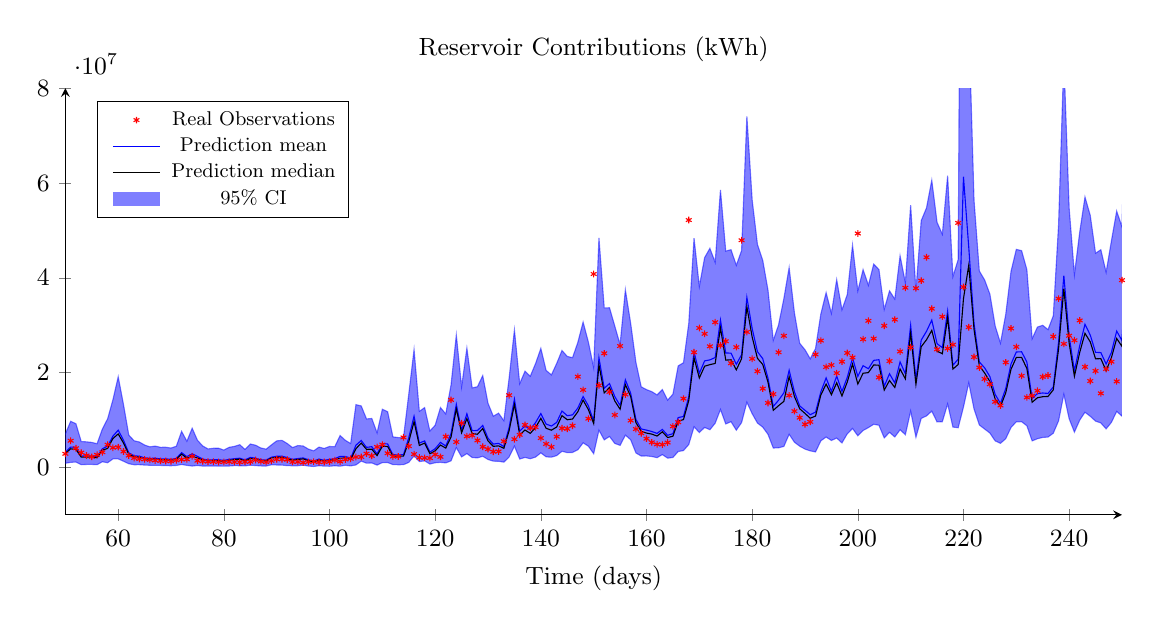
\begin{tikzpicture}


\begin{axis}[
	axis lines=left,
	font=\small,
	width=15cm,
	height=7cm,
%	axis background/.style={fill=background_color},
%	axis line style={white},
%	tick align=inside,
%	tick pos=left,
%	x grid style={white},
%	y grid style={white},
%	xmajorgrids,
%	ymajorgrids,
	title={Reservoir Contributions (kWh)},
	xlabel={Time (days)},
	xmin=50, xmax=250,
%	xtick style={color=black},
	ymin=-10000000, % Adjusted to -0.1*10^8
	ymax=80000000,  % Adjusted to 0.8*10^8
%	ytick style={color=black},
%	ytick={-10000000,0,20000000,40000000,60000000,80000000}, % Updated ticks for new range
%	yticklabels={
%		\ensuremath{-}0.1,
%		0.0,
%		0.2,
%		0.4,
%		0.6,
%		0.8
%	},
	legend columns=1, 
	legend style={
		nodes={scale=0.8, transform shape},
		fill opacity=0.8,
		draw opacity=1,
		text opacity=1,
		at={(0.03,0.97)},
		anchor=north west,
		legend pos=north west,
%		draw=lightgray204,
%		fill=background_color
	}
	]

\path [draw=blue, fill=blue, opacity=0.5]
(axis cs:0,30907406.4514597)
--(axis cs:0,5885922.78993782)
--(axis cs:1,5674543.05807476)
--(axis cs:2,7301785.31760189)
--(axis cs:3,6956792.82687586)
--(axis cs:4,8183185.13398946)
--(axis cs:5,8195896.04875933)
--(axis cs:6,8977533.45208891)
--(axis cs:7,9019784.38992647)
--(axis cs:8,6563541.59216855)
--(axis cs:9,5024031.82018058)
--(axis cs:10,3951316.81423389)
--(axis cs:11,3403244.46128388)
--(axis cs:12,3782391.59382283)
--(axis cs:13,3504576.48729532)
--(axis cs:14,2707612.09794435)
--(axis cs:15,3163042.44660711)
--(axis cs:16,3974093.56616021)
--(axis cs:17,5852836.73089923)
--(axis cs:18,4263134.95795006)
--(axis cs:19,3959661.0661793)
--(axis cs:20,3964063.41803515)
--(axis cs:21,3525253.3595841)
--(axis cs:22,1978248.24136687)
--(axis cs:23,1930215.12969607)
--(axis cs:24,1795470.67961426)
--(axis cs:25,1521195.59313902)
--(axis cs:26,1741044.87681918)
--(axis cs:27,1501987.83486739)
--(axis cs:28,1175185.73026311)
--(axis cs:29,1396483.47880615)
--(axis cs:30,949149.462315896)
--(axis cs:31,1123228.24390233)
--(axis cs:32,818526.291392528)
--(axis cs:33,937686.908303233)
--(axis cs:34,737592.724089867)
--(axis cs:35,813494.274872942)
--(axis cs:36,960671.555528153)
--(axis cs:37,860559.099717059)
--(axis cs:38,1066637.65883783)
--(axis cs:39,880174.293292029)
--(axis cs:40,1203749.6207275)
--(axis cs:41,799299.435247251)
--(axis cs:42,1041410.8596224)
--(axis cs:43,1122440.68145136)
--(axis cs:44,1185025.34164734)
--(axis cs:45,1068031.32659201)
--(axis cs:46,976186.989842073)
--(axis cs:47,625172.089805166)
--(axis cs:48,670027.717485929)
--(axis cs:49,1184285.79550688)
--(axis cs:50,883777.483314366)
--(axis cs:51,1066163.18486263)
--(axis cs:52,1140114.9025892)
--(axis cs:53,575074.852245501)
--(axis cs:54,626863.146294142)
--(axis cs:55,632801.920292059)
--(axis cs:56,578851.716113477)
--(axis cs:57,1196437.80523812)
--(axis cs:58,989773.072905666)
--(axis cs:59,1797140.29591263)
--(axis cs:60,1798154.77964696)
--(axis cs:61,1304855.40957626)
--(axis cs:62,779553.20094473)
--(axis cs:63,569662.222496089)
--(axis cs:64,578825.174967114)
--(axis cs:65,500652.438646471)
--(axis cs:66,448378.423212281)
--(axis cs:67,420966.139404685)
--(axis cs:68,416336.675522104)
--(axis cs:69,388884.452952956)
--(axis cs:70,351795.021472162)
--(axis cs:71,416945.249087078)
--(axis cs:72,621184.216491492)
--(axis cs:73,437569.654576349)
--(axis cs:74,291952.967227485)
--(axis cs:75,406831.279136508)
--(axis cs:76,286448.731488487)
--(axis cs:77,307267.713257018)
--(axis cs:78,310281.944410744)
--(axis cs:79,291076.089038305)
--(axis cs:80,284069.499330887)
--(axis cs:81,298451.884961761)
--(axis cs:82,377695.916852841)
--(axis cs:83,354547.143998929)
--(axis cs:84,321760.601013329)
--(axis cs:85,468192.91339697)
--(axis cs:86,393200.776244804)
--(axis cs:87,312057.91216927)
--(axis cs:88,295412.833710447)
--(axis cs:89,554706.917688585)
--(axis cs:90,516360.598094657)
--(axis cs:91,494111.100014269)
--(axis cs:92,370889.854193524)
--(axis cs:93,358099.934615687)
--(axis cs:94,358539.275531733)
--(axis cs:95,468705.953740391)
--(axis cs:96,295965.310266312)
--(axis cs:97,197864.488907552)
--(axis cs:98,356521.415093029)
--(axis cs:99,276908.054028984)
--(axis cs:100,253172.4422219)
--(axis cs:101,350615.41508964)
--(axis cs:102,266061.615309853)
--(axis cs:103,449415.0290544)
--(axis cs:104,322254.859010478)
--(axis cs:105,524458.209057414)
--(axis cs:106,1334293.54515099)
--(axis cs:107,896890.548558071)
--(axis cs:108,948184.657988197)
--(axis cs:109,484743.186544185)
--(axis cs:110,1018441.13138522)
--(axis cs:111,1031671.3502079)
--(axis cs:112,597977.644558914)
--(axis cs:113,569193.262254381)
--(axis cs:114,579148.38560621)
--(axis cs:115,1062122.20096183)
--(axis cs:116,2465459.77493679)
--(axis cs:117,1234431.38923625)
--(axis cs:118,1383804.85495062)
--(axis cs:119,712382.348651562)
--(axis cs:120,985623.702975463)
--(axis cs:121,1065269.3816668)
--(axis cs:122,954909.247549378)
--(axis cs:123,1391683.66143444)
--(axis cs:124,4187814.01334828)
--(axis cs:125,2217462.29546424)
--(axis cs:126,2921683.35272755)
--(axis cs:127,2092471.97076557)
--(axis cs:128,2013094.92666548)
--(axis cs:129,2347429.64240725)
--(axis cs:130,1678117.56757269)
--(axis cs:131,1319292.24769294)
--(axis cs:132,1293322.03081131)
--(axis cs:133,1116452.77034514)
--(axis cs:134,2206196.11739621)
--(axis cs:135,4494548.99962802)
--(axis cs:136,1770540.6675187)
--(axis cs:137,2105862.53864624)
--(axis cs:138,1837669.25303643)
--(axis cs:139,2179670.96744299)
--(axis cs:140,3074966.30594941)
--(axis cs:141,2234087.37280266)
--(axis cs:142,2161899.1783829)
--(axis cs:143,2490254.16821019)
--(axis cs:144,3409825.17436242)
--(axis cs:145,3119550.55482692)
--(axis cs:146,3153374.39827717)
--(axis cs:147,3712193.23046244)
--(axis cs:148,5194753.34239912)
--(axis cs:149,4470694.92589561)
--(axis cs:150,2897807.47054268)
--(axis cs:151,7859520.64788529)
--(axis cs:152,5807236.26266111)
--(axis cs:153,6537234.69029279)
--(axis cs:154,5060620.91715702)
--(axis cs:155,4654802.77415325)
--(axis cs:156,6807040.69104126)
--(axis cs:157,5846368.87004621)
--(axis cs:158,3049321.67459329)
--(axis cs:159,2407199.20059873)
--(axis cs:160,2423266.93220722)
--(axis cs:161,2304686.08890137)
--(axis cs:162,2056799.04374939)
--(axis cs:163,2710417.98343284)
--(axis cs:164,1950640.59611637)
--(axis cs:165,2108626.80029966)
--(axis cs:166,3355919.31777448)
--(axis cs:167,3554253.21428481)
--(axis cs:168,4825345.21652113)
--(axis cs:169,8583443.04109458)
--(axis cs:170,7352386.69048913)
--(axis cs:171,8438919.30352168)
--(axis cs:172,7959027.84575208)
--(axis cs:173,9323736.16401268)
--(axis cs:174,12226641.1956416)
--(axis cs:175,9168070.65343566)
--(axis cs:176,9646519.74676877)
--(axis cs:177,7853798.91381352)
--(axis cs:178,9462950.47762435)
--(axis cs:179,13748834.5005414)
--(axis cs:180,11334287.0340279)
--(axis cs:181,9365122.73363676)
--(axis cs:182,8500298.65753706)
--(axis cs:183,6974809.83608806)
--(axis cs:184,4093380.09949642)
--(axis cs:185,4137784.01428194)
--(axis cs:186,4428680.53816348)
--(axis cs:187,6991351.65173873)
--(axis cs:188,5315324.82770793)
--(axis cs:189,4472481.41795101)
--(axis cs:190,3868805.84633733)
--(axis cs:191,3487904.20338225)
--(axis cs:192,3269921.01495045)
--(axis cs:193,5610934.16841571)
--(axis cs:194,6409566.46787521)
--(axis cs:195,5683457.85231325)
--(axis cs:196,6197642.06216503)
--(axis cs:197,5168836.20709938)
--(axis cs:198,7081783.41341364)
--(axis cs:199,8222176.50188293)
--(axis cs:200,6672683.07126275)
--(axis cs:201,7789608.95212143)
--(axis cs:202,8400243.36157936)
--(axis cs:203,9101659.25258377)
--(axis cs:204,8895883.87374998)
--(axis cs:205,6233890.2294476)
--(axis cs:206,7398549.90511274)
--(axis cs:207,6430356.26271581)
--(axis cs:208,7940391.41339114)
--(axis cs:209,6901018.81867239)
--(axis cs:210,11895836.1328784)
--(axis cs:211,6356548.59057485)
--(axis cs:212,10338172.6082507)
--(axis cs:213,10861931.1816734)
--(axis cs:214,11872467.3086382)
--(axis cs:215,9594892.87895865)
--(axis cs:216,9642674.81646281)
--(axis cs:217,13395779.6000364)
--(axis cs:218,8513769.7207618)
--(axis cs:219,8369877.68060045)
--(axis cs:220,12742191.1041494)
--(axis cs:221,17844527.5247142)
--(axis cs:222,12309350.2711541)
--(axis cs:223,8961720.65478013)
--(axis cs:224,8095881.73521033)
--(axis cs:225,7246445.98931923)
--(axis cs:226,5600278.62800738)
--(axis cs:227,5078266.29217994)
--(axis cs:228,6061725.77955029)
--(axis cs:229,8427322.37777764)
--(axis cs:230,9633530.8166702)
--(axis cs:231,9647537.97854844)
--(axis cs:232,8791207.46929713)
--(axis cs:233,5594834.67091531)
--(axis cs:234,6054270.84717083)
--(axis cs:235,6330371.29844263)
--(axis cs:236,6401054.58601598)
--(axis cs:237,7212764.8196859)
--(axis cs:238,9809815.68165749)
--(axis cs:239,15428721.5136098)
--(axis cs:240,10279396.2328681)
--(axis cs:241,7452596.29537626)
--(axis cs:242,9960130.84129409)
--(axis cs:243,11638915.7063169)
--(axis cs:244,10789041.8465765)
--(axis cs:245,9759680.11014523)
--(axis cs:246,9381321.64545867)
--(axis cs:247,8131430.18191267)
--(axis cs:248,9502108.30393242)
--(axis cs:249,11816373.1473228)
--(axis cs:250,10810543.4266018)
--(axis cs:251,18182887.3666676)
--(axis cs:252,25668170.5000103)
--(axis cs:253,23414250.6982734)
--(axis cs:254,12249167.6070946)
--(axis cs:255,13146536.9276894)
--(axis cs:256,13211775.666662)
--(axis cs:257,10956399.719752)
--(axis cs:258,13905908.41429)
--(axis cs:259,10229376.6760242)
--(axis cs:260,13749834.7425519)
--(axis cs:261,13502351.9181865)
--(axis cs:262,10952763.5736677)
--(axis cs:263,16911381.3101086)
--(axis cs:264,18048853.6073122)
--(axis cs:265,13540809.8481116)
--(axis cs:266,11088934.1988711)
--(axis cs:267,11440076.0192202)
--(axis cs:268,8479460.79407775)
--(axis cs:269,6496459.88255137)
--(axis cs:270,7511496.97898794)
--(axis cs:271,13871495.3357715)
--(axis cs:272,13218869.7271439)
--(axis cs:273,11306477.0735967)
--(axis cs:274,9073863.72767941)
--(axis cs:275,7243336.22443831)
--(axis cs:276,9016953.15442407)
--(axis cs:277,8415278.38614876)
--(axis cs:278,10947933.3322801)
--(axis cs:279,6998521.75621858)
--(axis cs:280,6909559.10969476)
--(axis cs:281,7379816.54111927)
--(axis cs:282,8080349.87329687)
--(axis cs:283,9636050.27412812)
--(axis cs:284,6674818.28170529)
--(axis cs:285,5643060.0877621)
--(axis cs:286,5190403.02260596)
--(axis cs:287,5007120.39754427)
--(axis cs:288,4631625.70947617)
--(axis cs:289,6368279.23901656)
--(axis cs:290,5961320.00721586)
--(axis cs:291,6676578.92018345)
--(axis cs:292,5439848.93986802)
--(axis cs:293,4599629.60502644)
--(axis cs:294,4618721.54446433)
--(axis cs:295,3571849.92165438)
--(axis cs:296,4048967.16713747)
--(axis cs:297,3441618.84813054)
--(axis cs:298,3219848.44612806)
--(axis cs:299,3696846.96266786)
--(axis cs:300,3247579.25179106)
--(axis cs:301,3283952.03138324)
--(axis cs:302,4642174.53896253)
--(axis cs:303,10102445.1414483)
--(axis cs:304,10170619.0929285)
--(axis cs:305,6666880.56787654)
--(axis cs:306,5067312.83377437)
--(axis cs:307,4400712.87731744)
--(axis cs:308,5042738.62250831)
--(axis cs:309,5013968.83767498)
--(axis cs:310,4029528.35661837)
--(axis cs:311,4385369.73331181)
--(axis cs:312,4596221.72229076)
--(axis cs:313,3508063.15146899)
--(axis cs:314,5431127.44258737)
--(axis cs:315,5351588.39306578)
--(axis cs:316,7362632.67197411)
--(axis cs:317,9420654.0854381)
--(axis cs:318,5682107.72658379)
--(axis cs:319,4256823.8750039)
--(axis cs:320,4697740.15697164)
--(axis cs:321,5707905.18248479)
--(axis cs:322,3883883.97735439)
--(axis cs:323,3918063.66695527)
--(axis cs:324,3335132.94007076)
--(axis cs:325,3143126.46797185)
--(axis cs:326,3245422.54779617)
--(axis cs:327,4002944.84741737)
--(axis cs:328,5611325.11617583)
--(axis cs:329,6662831.56306687)
--(axis cs:330,4380736.90980662)
--(axis cs:331,3640388.39934131)
--(axis cs:332,3298331.89462565)
--(axis cs:333,3450353.22629363)
--(axis cs:334,3756787.12673499)
--(axis cs:335,3632144.96065723)
--(axis cs:336,3173995.28178716)
--(axis cs:337,2936465.30958241)
--(axis cs:338,5688568.66478927)
--(axis cs:339,6354918.27897763)
--(axis cs:340,3612129.24388249)
--(axis cs:341,3655025.41338249)
--(axis cs:342,3946968.45189771)
--(axis cs:343,5373970.37347272)
--(axis cs:344,3384818.16340067)
--(axis cs:345,2699665.40736224)
--(axis cs:346,2821564.70720534)
--(axis cs:347,2727266.92077257)
--(axis cs:348,5758722.19064767)
--(axis cs:349,7596014.62233575)
--(axis cs:350,7443577.35666882)
--(axis cs:351,8356835.84293042)
--(axis cs:352,9627219.46011807)
--(axis cs:353,6845695.51505982)
--(axis cs:354,6065686.37170465)
--(axis cs:355,5708725.78605777)
--(axis cs:356,9203669.97008046)
--(axis cs:357,10651545.9824798)
--(axis cs:358,7059257.49950107)
--(axis cs:359,5729878.43461214)
--(axis cs:360,5346773.13236028)
--(axis cs:361,4986651.28279049)
--(axis cs:362,4858615.43991823)
--(axis cs:363,3635066.5917467)
--(axis cs:364,3261658.97302984)
--(axis cs:365,2729343.78025953)
--(axis cs:366,2393662.33304993)
--(axis cs:367,2397017.93032576)
--(axis cs:368,2183968.85073964)
--(axis cs:369,1561968.27568165)
--(axis cs:370,1504705.38734753)
--(axis cs:371,1115345.94915297)
--(axis cs:372,1548269.14966113)
--(axis cs:373,1725084.35071295)
--(axis cs:374,1637833.16178425)
--(axis cs:375,2253411.33341079)
--(axis cs:376,4063904.38212003)
--(axis cs:377,3893908.94085638)
--(axis cs:378,5503964.55824355)
--(axis cs:379,3655975.40685349)
--(axis cs:380,2837472.92147622)
--(axis cs:381,1975589.69351533)
--(axis cs:382,2074520.1697708)
--(axis cs:383,1569034.66048513)
--(axis cs:384,1593125.1907466)
--(axis cs:385,1188698.67094589)
--(axis cs:386,1258446.03761076)
--(axis cs:387,1129419.84001063)
--(axis cs:388,997809.681282995)
--(axis cs:389,1047942.25675551)
--(axis cs:390,1034396.71414504)
--(axis cs:391,834479.349800151)
--(axis cs:392,923140.32875804)
--(axis cs:393,782335.914563685)
--(axis cs:394,1019495.0995653)
--(axis cs:395,859245.071988825)
--(axis cs:396,929741.013921958)
--(axis cs:397,582710.68067314)
--(axis cs:398,564277.115197866)
--(axis cs:399,765149.908633839)
--(axis cs:400,662383.531390484)
--(axis cs:401,790968.714943065)
--(axis cs:402,656868.530271685)
--(axis cs:403,712265.826661303)
--(axis cs:404,956314.743010091)
--(axis cs:405,982663.792073087)
--(axis cs:406,776901.887679556)
--(axis cs:407,640899.799539382)
--(axis cs:408,623205.05472591)
--(axis cs:409,968760.52056564)
--(axis cs:410,972558.038259843)
--(axis cs:411,928068.87001041)
--(axis cs:412,1023035.3434562)
--(axis cs:413,873814.437637977)
--(axis cs:414,653636.052045234)
--(axis cs:415,784966.294567908)
--(axis cs:416,785282.572579655)
--(axis cs:417,666827.845717447)
--(axis cs:418,518345.578987251)
--(axis cs:419,505802.962987898)
--(axis cs:420,537978.068505467)
--(axis cs:421,639022.101410031)
--(axis cs:422,552775.651046558)
--(axis cs:423,507323.168394768)
--(axis cs:424,484162.927752758)
--(axis cs:425,404238.958893168)
--(axis cs:426,488064.294943239)
--(axis cs:427,449202.257629827)
--(axis cs:428,658603.676186485)
--(axis cs:429,469330.385086818)
--(axis cs:430,371638.602575499)
--(axis cs:431,512666.39473428)
--(axis cs:432,454228.701608211)
--(axis cs:433,374808.909598031)
--(axis cs:434,345175.884406033)
--(axis cs:435,397675.743865078)
--(axis cs:436,562026.310520272)
--(axis cs:437,514053.464560066)
--(axis cs:438,331948.934847177)
--(axis cs:439,771993.608710197)
--(axis cs:440,425095.600541194)
--(axis cs:440,4199289.41172533)
--(axis cs:440,4199289.41172533)
--(axis cs:439,5263544.99962118)
--(axis cs:438,3818942.60412088)
--(axis cs:437,4618188.69990215)
--(axis cs:436,4728135.30626294)
--(axis cs:435,4052103.13101315)
--(axis cs:434,4133688.57304111)
--(axis cs:433,3986905.48424963)
--(axis cs:432,4266202.43738488)
--(axis cs:431,4639610.26834708)
--(axis cs:430,4086673.67146971)
--(axis cs:429,4630651.88498612)
--(axis cs:428,5909738.08595537)
--(axis cs:427,4291683.26714343)
--(axis cs:426,4430276.03212385)
--(axis cs:425,4146270.05640581)
--(axis cs:424,4379158.57181653)
--(axis cs:423,4468609.3331454)
--(axis cs:422,4658124.13311879)
--(axis cs:421,4824686.54011011)
--(axis cs:420,4510879.42990366)
--(axis cs:419,4553589.50305825)
--(axis cs:418,4422728.93501595)
--(axis cs:417,4851426.62973183)
--(axis cs:416,5614774.7346897)
--(axis cs:415,5526964.00691462)
--(axis cs:414,5470393.57455906)
--(axis cs:413,5926840.43958532)
--(axis cs:412,6208355.04309339)
--(axis cs:411,5968121.02158074)
--(axis cs:410,5884214.47079459)
--(axis cs:409,6025731.40357646)
--(axis cs:408,4987703.05070686)
--(axis cs:407,5308124.66512419)
--(axis cs:406,5767149.89908403)
--(axis cs:405,6474017.77728772)
--(axis cs:404,6406287.84291345)
--(axis cs:403,5877550.19988039)
--(axis cs:402,5655336.47440097)
--(axis cs:401,6099774.67390184)
--(axis cs:400,5291037.08656023)
--(axis cs:399,6130470.43969601)
--(axis cs:398,5258439.13700402)
--(axis cs:397,5250051.64528962)
--(axis cs:396,8007819.0213936)
--(axis cs:395,6382625.3894454)
--(axis cs:394,6810077.26067491)
--(axis cs:393,5738505.43750242)
--(axis cs:392,6509519.83214562)
--(axis cs:391,6256760.80901626)
--(axis cs:390,7268595.62931472)
--(axis cs:389,7176817.46126866)
--(axis cs:388,7420154.99863558)
--(axis cs:387,8203979.65226962)
--(axis cs:386,8208120.54934509)
--(axis cs:385,8527250.74451589)
--(axis cs:384,10114216.0523928)
--(axis cs:383,10077226.1671876)
--(axis cs:382,12515729.3942162)
--(axis cs:381,12029744.16748)
--(axis cs:380,18382389.4497451)
--(axis cs:379,21931659.4898066)
--(axis cs:378,32119867.070031)
--(axis cs:377,20820209.8705683)
--(axis cs:376,24948150.4232784)
--(axis cs:375,13294629.1234139)
--(axis cs:374,10965545.7905627)
--(axis cs:373,11314382.9071257)
--(axis cs:372,10593742.0637399)
--(axis cs:371,8576076.23809106)
--(axis cs:370,9069698.93993837)
--(axis cs:369,9485139.24966531)
--(axis cs:368,12852205.4554322)
--(axis cs:367,13762894.4832561)
--(axis cs:366,13687612.4645395)
--(axis cs:365,15566675.848878)
--(axis cs:364,17061337.2891881)
--(axis cs:363,19664924.6194977)
--(axis cs:362,25144748.6747629)
--(axis cs:361,24232926.5112259)
--(axis cs:360,25016658.7708773)
--(axis cs:359,26422032.2018139)
--(axis cs:358,32996183.5984118)
--(axis cs:357,47398028.8214451)
--(axis cs:356,40219331.6917484)
--(axis cs:355,28905967.3930454)
--(axis cs:354,32007322.0913327)
--(axis cs:353,31985076.1367082)
--(axis cs:352,43111394.2949487)
--(axis cs:351,37219593.2611589)
--(axis cs:350,36268949.2467646)
--(axis cs:349,36098827.4871247)
--(axis cs:348,32821909.2721048)
--(axis cs:347,15787497.5914623)
--(axis cs:346,16445861.5089191)
--(axis cs:345,14812096.2438514)
--(axis cs:344,18756905.9335852)
--(axis cs:343,30971165.7016194)
--(axis cs:342,22302483.5983266)
--(axis cs:341,20993698.1816097)
--(axis cs:340,20348169.9786559)
--(axis cs:339,33284668.8577015)
--(axis cs:338,33237255.123715)
--(axis cs:337,17936012.1471995)
--(axis cs:336,18016255.2876366)
--(axis cs:335,18959121.8845204)
--(axis cs:334,21275356.8717298)
--(axis cs:333,22358248.7255727)
--(axis cs:332,19026992.0625653)
--(axis cs:331,20314532.2896306)
--(axis cs:330,24161823.2796418)
--(axis cs:329,37377306.3708081)
--(axis cs:328,34282242.611517)
--(axis cs:327,24366583.5055708)
--(axis cs:326,18149451.0588443)
--(axis cs:325,18191804.0407082)
--(axis cs:324,19769761.1426609)
--(axis cs:323,22918496.4287368)
--(axis cs:322,22929127.0902387)
--(axis cs:321,29626099.0200389)
--(axis cs:320,23163977.3193191)
--(axis cs:319,21877404.9032236)
--(axis cs:318,28570111.2474229)
--(axis cs:317,42804253.2748846)
--(axis cs:316,36196246.8076043)
--(axis cs:315,36674359.4645165)
--(axis cs:314,31421425.1906672)
--(axis cs:313,21217535.1550024)
--(axis cs:312,22553204.4858835)
--(axis cs:311,22101177.0678996)
--(axis cs:310,20993247.0917678)
--(axis cs:309,25858639.8454585)
--(axis cs:308,25264769.7295539)
--(axis cs:307,23365468.291973)
--(axis cs:306,26392697.1962685)
--(axis cs:305,35255657.2822883)
--(axis cs:304,45904336.2582476)
--(axis cs:303,49064582.6554454)
--(axis cs:302,27899613.7706029)
--(axis cs:301,19496350.7354926)
--(axis cs:300,18904851.617763)
--(axis cs:299,20863260.8189016)
--(axis cs:298,19989921.1833747)
--(axis cs:297,20731501.2251396)
--(axis cs:296,21875505.3174502)
--(axis cs:295,20617078.4280775)
--(axis cs:294,25773286.5491508)
--(axis cs:293,29997732.4868623)
--(axis cs:292,30877926.3490141)
--(axis cs:291,32257968.4820293)
--(axis cs:290,32282313.1228062)
--(axis cs:289,37502244.6044886)
--(axis cs:288,27348258.8395536)
--(axis cs:287,27813690.4435484)
--(axis cs:286,27002598.9074423)
--(axis cs:285,29326763.3269021)
--(axis cs:284,33061960.5431371)
--(axis cs:283,44810607.6673006)
--(axis cs:282,38839697.0114324)
--(axis cs:281,39548602.7998612)
--(axis cs:280,36969658.6218567)
--(axis cs:279,38966399.2340311)
--(axis cs:278,59325482.663408)
--(axis cs:277,39858016.07084)
--(axis cs:276,42014756.5951939)
--(axis cs:275,38124287.3146453)
--(axis cs:274,46059938.7169577)
--(axis cs:273,49881722.1286587)
--(axis cs:272,56914531.8272636)
--(axis cs:271,73079825.3809388)
--(axis cs:270,32375885.3533778)
--(axis cs:269,28433886.9913605)
--(axis cs:268,34480946.230896)
--(axis cs:267,47154270.6506619)
--(axis cs:266,44160137.7425085)
--(axis cs:265,58089025.7558108)
--(axis cs:264,78333884.5980151)
--(axis cs:263,68816427.0143886)
--(axis cs:262,47470360.2480301)
--(axis cs:261,56747625.9222415)
--(axis cs:260,63250019.5038976)
--(axis cs:259,48845449.5107154)
--(axis cs:258,58811523.6211435)
--(axis cs:257,48893925.3812921)
--(axis cs:256,57910547.9343189)
--(axis cs:255,56681689.1139916)
--(axis cs:254,51247492.3237838)
--(axis cs:253,119579645.037083)
--(axis cs:252,305785769.363122)
--(axis cs:251,93327319.9002433)
--(axis cs:250,50756456.9957249)
--(axis cs:249,54073495.033407)
--(axis cs:248,47756510.6623956)
--(axis cs:247,41158152.994058)
--(axis cs:246,45924689.6402783)
--(axis cs:245,45185173.0286492)
--(axis cs:244,53157935.394833)
--(axis cs:243,57040752.9040771)
--(axis cs:242,49593942.0901391)
--(axis cs:241,40671142.563746)
--(axis cs:240,54778407.4952251)
--(axis cs:239,86206805.1205929)
--(axis cs:238,51149787.9960311)
--(axis cs:237,31982658.7044678)
--(axis cs:236,29061661.9785873)
--(axis cs:235,29983347.3115835)
--(axis cs:234,29605645.9352351)
--(axis cs:233,27147369.9770555)
--(axis cs:232,41730796.2947655)
--(axis cs:231,45727997.4309129)
--(axis cs:230,45993485.0198137)
--(axis cs:229,41338497.6753431)
--(axis cs:228,32287820.9056374)
--(axis cs:227,26211792.5515864)
--(axis cs:226,29856739.813329)
--(axis cs:225,36558914.4728581)
--(axis cs:224,39561108.8255466)
--(axis cs:223,41430871.6979982)
--(axis cs:222,56331651.5976199)
--(axis cs:221,94489742.6225434)
--(axis cs:220,238728692.658533)
--(axis cs:219,43860154.7920334)
--(axis cs:218,40256613.7793458)
--(axis cs:217,61529186.099065)
--(axis cs:216,49180430.2715794)
--(axis cs:215,51696071.3398773)
--(axis cs:214,60579010.4360006)
--(axis cs:213,54738534.6118452)
--(axis cs:212,52057275.3123109)
--(axis cs:211,37252920.7073407)
--(axis cs:210,55323960.7667376)
--(axis cs:209,38957899.1281953)
--(axis cs:208,44643183.5954432)
--(axis cs:207,35501894.8048815)
--(axis cs:206,37247947.5079995)
--(axis cs:205,33347775.6830233)
--(axis cs:204,41750122.8307517)
--(axis cs:203,42883287.5820727)
--(axis cs:202,38415374.5349056)
--(axis cs:201,41729699.734216)
--(axis cs:200,37240659.001287)
--(axis cs:199,46862055.7254133)
--(axis cs:198,36458114.0304558)
--(axis cs:197,33249517.6092754)
--(axis cs:196,39595135.8804486)
--(axis cs:195,32508123.0477923)
--(axis cs:194,36862176.2543281)
--(axis cs:193,32365151.0246501)
--(axis cs:192,25105088.2294362)
--(axis cs:191,22903797.8731198)
--(axis cs:190,24826961.7395492)
--(axis cs:189,26177037.6405506)
--(axis cs:188,32606151.7361513)
--(axis cs:187,42149932.4141385)
--(axis cs:186,35605431.2187158)
--(axis cs:185,30071075.7194126)
--(axis cs:184,26808768.2281718)
--(axis cs:183,37379003.3201648)
--(axis cs:182,43715898.5868172)
--(axis cs:181,47041899.3997055)
--(axis cs:180,56451508.3282476)
--(axis cs:179,74059373.3070983)
--(axis cs:178,45741177.7066333)
--(axis cs:177,42628409.3226226)
--(axis cs:176,45925586.2285622)
--(axis cs:175,45635323.8654739)
--(axis cs:174,58526888.4029096)
--(axis cs:173,43252798.7037189)
--(axis cs:172,46219241.4597439)
--(axis cs:171,44248732.8907601)
--(axis cs:170,38167804.8096629)
--(axis cs:169,48360630.5680163)
--(axis cs:168,30380202.9341655)
--(axis cs:167,22075636.8426656)
--(axis cs:166,21417404.9796468)
--(axis cs:165,15449271.2575766)
--(axis cs:164,14193505.2428978)
--(axis cs:163,16410203.2887796)
--(axis cs:162,15293227.4690749)
--(axis cs:161,15988802.8175019)
--(axis cs:160,16410006.6267682)
--(axis cs:159,17006613.5068585)
--(axis cs:158,22148215.8249944)
--(axis cs:157,30412818.7667384)
--(axis cs:156,37451413.0768894)
--(axis cs:155,25907320.4800542)
--(axis cs:154,29796321.8137097)
--(axis cs:153,33675433.1359814)
--(axis cs:152,33651699.566187)
--(axis cs:151,48399966.3322372)
--(axis cs:150,21043173.7399156)
--(axis cs:149,26437965.7828873)
--(axis cs:148,30659116.8284679)
--(axis cs:147,26370942.4893997)
--(axis cs:146,23154414.7396531)
--(axis cs:145,23407901.3196011)
--(axis cs:144,24662706.2701574)
--(axis cs:143,21932521.3781466)
--(axis cs:142,19513936.2353838)
--(axis cs:141,20461046.5476423)
--(axis cs:140,25103300.2639423)
--(axis cs:139,21912393.5078485)
--(axis cs:138,19231517.9150977)
--(axis cs:137,20288123.8723443)
--(axis cs:136,17659691.892833)
--(axis cs:135,28992565.606704)
--(axis cs:134,18909537.0122337)
--(axis cs:133,9846382.82989278)
--(axis cs:132,11443441.0379957)
--(axis cs:131,10800821.2126233)
--(axis cs:130,13530505.3159609)
--(axis cs:129,19360701.8583425)
--(axis cs:128,17021778.2061125)
--(axis cs:127,16766165.6684989)
--(axis cs:126,25152410.3523359)
--(axis cs:125,16988109.2911192)
--(axis cs:124,27920254.6201206)
--(axis cs:123,17385837.2854033)
--(axis cs:122,11276396.7988257)
--(axis cs:121,12630869.7752584)
--(axis cs:120,8901250.0818607)
--(axis cs:119,7668918.75883771)
--(axis cs:118,12616812.0524451)
--(axis cs:117,11817036.3463745)
--(axis cs:116,24852128.2608868)
--(axis cs:115,15463589.1890112)
--(axis cs:114,6297129.69147975)
--(axis cs:113,6293631.04049408)
--(axis cs:112,6439658.64207188)
--(axis cs:111,11755927.0095615)
--(axis cs:110,12269578.218331)
--(axis cs:109,7293472.90140121)
--(axis cs:108,10327909.2357345)
--(axis cs:107,10222168.2334478)
--(axis cs:106,12969254.8018652)
--(axis cs:105,13244789.1176147)
--(axis cs:104,5044976.20097081)
--(axis cs:103,5710747.26996729)
--(axis cs:102,6728089.9427976)
--(axis cs:101,4368750.58573883)
--(axis cs:100,4415523.74963993)
--(axis cs:99,4000092.37141886)
--(axis cs:98,4284010.08869339)
--(axis cs:97,3490376.60940341)
--(axis cs:96,3865187.75572023)
--(axis cs:95,4519671.4742157)
--(axis cs:94,4613062.24608463)
--(axis cs:93,4177861.27667571)
--(axis cs:92,5033785.94701024)
--(axis cs:91,5707540.58931229)
--(axis cs:90,5599455.31266141)
--(axis cs:89,4747961.61216315)
--(axis cs:88,3850863.80318259)
--(axis cs:87,4103481.71630969)
--(axis cs:86,4675993.77923644)
--(axis cs:85,4940873.40835879)
--(axis cs:84,3791606.47415043)
--(axis cs:83,4792824.65342116)
--(axis cs:82,4428362.75821313)
--(axis cs:81,4242658.82889773)
--(axis cs:80,3657509.10868021)
--(axis cs:79,4054534.82920661)
--(axis cs:78,4037710.36183407)
--(axis cs:77,3898448.61515546)
--(axis cs:76,4516804.16665704)
--(axis cs:75,5729245.3165944)
--(axis cs:74,8263451.89912157)
--(axis cs:73,5516158.77842074)
--(axis cs:72,7603119.96047562)
--(axis cs:71,4462300.92007251)
--(axis cs:70,4086342.9563068)
--(axis cs:69,4251436.98869144)
--(axis cs:68,4239491.38409234)
--(axis cs:67,4503542.3388013)
--(axis cs:66,4338614.14249858)
--(axis cs:65,4714606.74619845)
--(axis cs:64,5358833.73768554)
--(axis cs:63,5627121.03027346)
--(axis cs:62,6838349.51114454)
--(axis cs:61,13254043.2033068)
--(axis cs:60,19111471.0362781)
--(axis cs:59,14279685.6789195)
--(axis cs:58,10268089.8490413)
--(axis cs:57,8097279.19854255)
--(axis cs:56,4998346.9356354)
--(axis cs:55,5275477.89839847)
--(axis cs:54,5393959.72502817)
--(axis cs:53,5457645.64223258)
--(axis cs:52,9206202.37065737)
--(axis cs:51,9731647.30718806)
--(axis cs:50,7086408.94073138)
--(axis cs:49,9981135.63327471)
--(axis cs:48,5411792.86035991)
--(axis cs:47,5147326.35877483)
--(axis cs:46,6261454.67355194)
--(axis cs:45,6985651.31913097)
--(axis cs:44,7160892.75926486)
--(axis cs:43,6363552.28692704)
--(axis cs:42,6541472.34047879)
--(axis cs:41,5918323.0243611)
--(axis cs:40,6747156.21716429)
--(axis cs:39,6177516.19461915)
--(axis cs:38,7267928.26480801)
--(axis cs:37,5963307.52297306)
--(axis cs:36,6539234.16054271)
--(axis cs:35,5762756.94620261)
--(axis cs:34,5481795.56676344)
--(axis cs:33,6685318.96357387)
--(axis cs:32,5617334.43244526)
--(axis cs:31,8421154.50384803)
--(axis cs:30,6396627.25635895)
--(axis cs:29,9362920.18032182)
--(axis cs:28,7393880.28051603)
--(axis cs:27,9801266.61087961)
--(axis cs:26,10542239.2729267)
--(axis cs:25,9100827.61774091)
--(axis cs:24,10613262.965633)
--(axis cs:23,11461534.9194487)
--(axis cs:22,11383551.213304)
--(axis cs:21,18294344.5244007)
--(axis cs:20,20287612.7119578)
--(axis cs:19,19027300.8296004)
--(axis cs:18,20189562.5128942)
--(axis cs:17,28261813.569889)
--(axis cs:16,22987212.2921109)
--(axis cs:15,17012807.2491663)
--(axis cs:14,15427795.4761646)
--(axis cs:13,18200869.7162744)
--(axis cs:12,19240157.355112)
--(axis cs:11,17737071.6739917)
--(axis cs:10,20061172.1473353)
--(axis cs:9,26305564.9902142)
--(axis cs:8,29539023.8489169)
--(axis cs:7,43610232.6175159)
--(axis cs:6,44239662.2620842)
--(axis cs:5,40578806.3473961)
--(axis cs:4,44812877.4860693)
--(axis cs:3,35931535.608027)
--(axis cs:2,37271950.6111963)
--(axis cs:1,33355288.1255068)
--(axis cs:0,30907406.4514597)
--cycle;

\addplot [only marks, red, mark=asterisk, mark size=1.2]
table {%
0 17920100
1 20248400
2 18087300
3 18316900
4 18044700
5 22639100
6 19789300
7 14686600
8 11502400
9 9352700
10 8582100
11 11649900
12 9782300
13 7409700
14 7937700
15 11951600
16 13791300
17 10920300
18 10713700
19 12009000
20 11282600
21 7367100
22 6603000
23 6539000
24 5942200
25 5765100
26 5302700
27 4925600
28 4325500
29 3851600
30 3472800
31 3169500
32 3046500
33 3474500
34 3267900
35 3308900
36 3322000
37 3338400
38 2776000
39 2633300
40 2776000
41 2375900
42 2215200
43 2999000
44 2917000
45 2402100
46 2274200
47 2433300
48 4332000
49 2994100
50 2869400
51 5627400
52 4043500
53 3120300
54 2528400
55 2233200
56 2666100
57 3199000
58 4791100
59 4153300
60 4274600
61 3363000
62 2495600
63 1993900
64 1765900
65 1702000
66 1592100
67 1464200
68 1372400
69 1347800
70 1311700
71 1508500
72 1659400
73 1702000
74 2341500
75 1420000
76 1308500
77 1223200
78 1192000
79 1136300
80 1149400
81 1190400
82 1129700
83 1101900
84 1167500
85 1208400
86 1551100
87 1272400
88 1116600
89 1388800
90 1728200
91 1726600
92 1623300
93 1160900
94 1170700
95 1015000
96 1167500
97 1231400
98 1115000
99 1129700
100 1228100
101 1549500
102 1251100
103 1665900
104 1821700
105 2193900
106 2202100
107 2903900
108 2428400
109 4323800
110 4814100
111 2985900
112 2297200
113 2305400
114 6327500
115 4494400
116 2805500
117 2077500
118 2008600
119 1970900
120 2710400
121 2228300
122 6494800
123 14245500
124 5363400
125 9349500
126 6568600
127 6753800
128 5697900
129 4345200
130 3863100
131 3307200
132 3369500
133 5522400
134 15231000
135 5953700
136 6871900
137 8970700
138 8341100
139 8483700
140 6193100
141 4950200
142 4327100
143 6491500
144 8265600
145 8141000
146 8800200
147 19151500
148 16346000
149 10290600
150 40800200
151 17308500
152 24067200
153 15927900
154 11067800
155 25603600
156 15375300
157 9887300
158 8095100
159 7209700
160 6063500
161 5289600
162 4866600
163 4815700
164 5242100
165 8669000
166 9542900
167 14517700
168 52177900
169 24288600
170 29417500
171 28182800
172 25541300
173 30627600
174 25752800
175 26618600
176 21983200
177 25367500
178 47919600
179 28571400
180 22909600
181 20286100
182 16623100
183 13602800
184 15458900
185 24282000
186 27756500
187 15190000
188 11868000
189 10492300
190 9096900
191 9602000
192 23829500
193 26753000
194 21184700
195 21588000
196 19899200
197 22309500
198 24147600
199 23190000
200 49352700
201 27041600
202 30930900
203 27174400
204 18992400
205 29878200
206 22434100
207 31185100
208 24457500
209 37904500
210 25323200
211 37802800
212 39396600
213 44325500
214 33485500
215 24906700
216 31806500
217 25085500
218 25892200
219 51576100
220 38050400
221 29583100
222 23290000
223 21069900
224 18662800
225 17557700
226 13837300
227 13066600
228 22163600
229 29327300
230 25428200
231 19318700
232 14771900
233 15132600
234 16177100
235 19100600
236 19381000
237 27615500
238 35612200
239 26056200
240 27774500
241 26820200
242 31006300
243 21214200
244 18223400
245 20350100
246 15621200
247 20760000
248 22301300
249 18144700
250 39506400
251 46898100
252 64052500
253 37488000
254 39360500
255 33231400
256 27777800
257 25434700
258 24719800
259 41657700
260 29101000
261 22374000
262 43966500
263 44027000
264 36616400
265 30216200
266 28524100
267 20749000
268 16987300
269 23598500
270 36276400
271 27510500
272 35321700
273 29521400
274 22944500
275 22181100
276 26176500
277 35362500
278 25040400
279 25037100
280 22156600
281 19184500
282 27206500
283 17706600
284 15772600
285 11930800
286 11368500
287 10760300
288 32362700
289 14795000
290 18355600
291 17165500
292 13585300
293 10915600
294 10258400
295 9548900
296 8646500
297 8092300
298 7856900
299 7505400
300 7456400
301 9874200
302 37072500
303 43216100
304 14688700
305 10892700
306 10770100
307 12025600
308 11775500
309 9648600
310 8914600
311 9890600
312 8917900
313 12215300
314 35035600
315 21501000
316 23971200
317 14410800
318 10387600
319 9969100
320 14520400
321 12476900
322 10735800
323 8744600
324 7547900
325 7343600
326 8913000
327 17425400
328 13748700
329 10690000
330 9058500
331 7732600
332 10789700
333 9107500
334 7734300
335 7060700
336 7121200
337 12414700
338 16140500
339 8811600
340 7513600
341 7546300
342 11554800
343 9539100
344 8471600
345 8579500
346 7785000
347 18571400
348 21973500
349 23778300
350 23215900
351 34620300
352 21178900
353 13477400
354 15167700
355 29351300
356 44963800
357 20335400
358 14605400
359 12252900
360 10199600
361 15777500
362 9835000
363 9583200
364 8497700
365 7502100
366 7086900
367 7266700
368 6712500
369 6231900
370 5965400
371 5161100
372 9223600
373 6310400
374 5527300
375 8223100
376 10583700
377 12437600
378 10085100
379 7753900
380 6228600
381 5417800
382 5015600
383 3457600
384 3439600
385 3336600
386 3197700
387 3408600
388 3338300
389 3375900
390 3305600
391 3357900
392 3335000
393 2476700
394 3181300
395 3163400
396 2633700
397 2883800
398 2865800
399 2744800
400 2661500
401 2594400
402 2538900
403 2507800
404 2679500
405 2543800
406 2460400
407 2529000
408 2468600
409 2350900
410 2243000
411 1978100
412 1816300
413 1790100
414 1427200
415 1401000
416 1334000
417 1271900
418 1185200
419 1185200
420 1101900
421 1062600
422 1029900
423 1052800
424 1054500
425 1070800
426 1041400
427 1798300
428 1412500
429 1257200
430 1255500
431 1193400
432 1093700
433 1039700
434 951500
435 904000
436 874600
437 954700
438 994000
439 966200
440 948200
};
\addplot [blue]
table {%
0 15817166.9029387
1 17145190.5225306
2 19703475.5105783
3 18366736.5824923
4 22129341.9521366
5 21306174.908615
6 23187246.6687183
7 23371020.6348475
8 15896690.0053414
9 13741863.5486684
10 10424577.0164218
11 9080490.87441059
12 10013378.7443896
13 9182104.06261942
14 7846247.88242018
15 8595205.26428845
16 11511290.9300549
17 14899460.0106026
18 10670458.049483
19 9979722.79245217
20 10794865.9503605
21 9709820.95568015
22 5640538.97860684
23 5616153.9244689
24 5197156.93713589
25 4548266.10054598
26 5314543.00332894
27 4721815.68558829
28 3573737.71570562
29 4519775.75500272
30 3100719.75848485
31 3870869.16124664
32 2694471.66639465
33 3200701.2371607
34 2616177.07934864
35 2755737.97811234
36 3201327.49819082
37 2809819.71292162
38 3490717.52570412
39 2904829.74159846
40 3400483.45573234
41 2730737.02965754
42 3170535.39629684
43 3220589.57931373
44 3582313.62486965
45 3311635.31864139
46 3037045.60066886
47 2352686.80081
48 2499687.28697661
49 4538686.53775737
50 3224267.9289801
51 4285912.76483627
52 4238386.82476412
53 2391420.73346951
54 2417153.56286799
55 2391550.3385881
56 2223965.5403143
57 3943611.29506132
58 4484577.14456321
59 6602806.22063108
60 7862122.88719539
61 5732097.37389192
62 3052571.74047431
63 2451709.22492641
64 2364887.0271427
65 2007080.50751847
66 1908264.74471907
67 1941827.7473877
68 1813393.26031246
69 1806817.21795047
70 1689273.10304811
71 1898369.86212898
72 3109582.06755396
73 2258302.59010804
74 2874504.26571522
75 2317164.25553454
76 1761716.56760604
77 1565062.8292228
78 1614692.05972512
79 1612752.99904145
80 1475797.31956482
81 1694741.26618903
82 1847645.141592
83 1942621.24493914
84 1575096.52578418
85 2114560.76283538
86 1951151.33717167
87 1618964.81480327
88 1542587.96726445
89 2158072.71553427
90 2355808.13646589
91 2375383.76644832
92 2064138.4550911
93 1705341.59540626
94 1875553.09285395
95 1996577.57431946
96 1616251.69613577
97 1329501.32287569
98 1764291.54413542
99 1498404.07424741
100 1706750.81492763
101 1828069.79457661
102 2335417.30557071
103 2312260.3853618
104 1910045.63439667
105 4689766.24085449
106 5681508.23436574
107 4221029.90303453
108 4375039.47411462
109 2835057.11608126
110 5026304.10091156
111 4944164.04608513
112 2688040.45641937
113 2640485.54634326
114 2685431.78192499
115 6268336.11662248
116 10810267.7751976
117 5131443.81071823
118 5591279.25522077
119 3229836.56317685
120 3948910.39269931
121 5281301.48351834
122 4521541.23626272
123 7150497.90137576
124 13304132.8565417
125 7831691.15026142
126 11305386.2794738
127 7760746.66352563
128 7786368.01499926
129 8859583.31097712
130 6158088.54079236
131 4914631.07092061
132 5077495.31563268
133 4392648.03245461
134 8443942.0368202
135 14395306.8687438
136 7644108.8624477
137 8769869.23282104
138 7970041.60712091
139 9460650.0986257
140 11364259.721617
141 9141525.56233264
142 8729581.71874131
143 9502865.7819968
144 11889987.4793034
145 10914131.8706718
146 11087038.9307394
147 12520983.3460805
148 14958314.0298709
149 12990465.8431474
150 9781807.80972213
151 23117339.2727531
152 16691438.6513235
153 17690181.3809365
154 14947696.774802
155 13052704.4048142
156 18481656.5983629
157 15670104.684711
158 10114210.8777156
159 8118929.95797702
160 7869362.10966852
161 7575244.81212652
162 7178454.91680303
163 8019116.8496968
164 6772678.8687646
165 7111980.83840174
166 10513614.3091575
167 10751949.1640092
168 14902944.9211813
169 24369524.2102699
170 19842279.4558989
171 22469725.3368968
172 22684036.6355168
173 23185777.8241614
174 31098812.2636249
175 24130611.45815
176 24119749.950085
177 21744844.1856101
178 23781403.5908344
179 35846457.8776203
180 29300834.7852873
181 24429275.8890735
182 22947298.1274158
183 18822381.8122583
184 12850334.2635998
185 14190204.1007543
186 15717137.5875855
187 20493636.7845707
188 15969208.4300027
189 12965556.2345471
190 12059048.9434909
191 11115882.943589
192 11670584.380552
193 15945009.0818837
194 18883807.6422594
195 16031881.0225333
196 19278213.1580589
197 16035549.9606281
198 18984525.9336109
199 23109339.4407823
200 19203536.1529147
201 21460367.0913395
202 20813820.024191
203 22579939.7274051
204 22720952.2997906
205 17112860.0100969
206 19764576.7848033
207 17805341.6972037
208 22263459.3083684
209 19749110.7406204
210 29986885.1709166
211 18589813.6964119
212 26858300.2111651
213 28712323.1470952
214 31076024.7571954
215 26104543.7860655
216 25260201.6447637
217 32972642.9163986
218 21549993.9082119
219 22845599.0259692
220 61310619.5845119
221 46429670.0344703
222 30353582.8232426
223 22253140.9758421
224 21008577.2396638
225 19162323.4044949
226 15410261.0997889
227 13493714.5859948
228 16640599.2950091
229 21812942.3092414
230 24344877.2890107
231 24395789.1426938
232 22230274.5852992
233 14505771.4005165
234 15578556.29157
235 15699371.558797
236 15608658.4668774
237 16972435.9899214
238 26397340.9133122
239 40463018.6028649
240 27693970.2287068
241 20374161.1848208
242 25642702.3162933
243 30207771.8296936
244 27912000.6090829
245 24282004.4819338
246 24218980.0735596
247 21813125.0750976
248 24251126.6147131
249 28757133.215754
250 26763331.5055557
251 47589853.6306894
252 85876621.7765533
253 59640960.0422263
254 28236662.3118587
255 30941156.7329272
256 31712491.2340658
257 26116171.5182185
258 32278329.3513308
259 25948446.4489517
260 34185380.1474541
261 31476736.7663939
262 25867181.1734402
263 38561932.7340806
264 42004420.431799
265 32089234.4417422
266 25070680.1878136
267 26090450.0579419
268 19340712.3791421
269 15382610.9820694
270 17908802.8710566
271 35853662.7616761
272 31031921.0115907
273 27239953.6316347
274 24039254.1785751
275 19728196.3418067
276 22516160.4085836
277 21549256.3199576
278 28517092.6667087
279 19985147.0645098
280 18780448.392693
281 20361337.2777619
282 20593379.2603232
283 24294555.8596071
284 17305416.1559645
285 15022872.467961
286 13953284.3598747
287 14018742.5673007
288 13742789.7099644
289 18142349.1759614
290 16558625.4635079
291 17126433.2227616
292 15670226.8263745
293 14489078.3597249
294 13195014.9273231
295 10221924.3231966
296 11005332.6689434
297 10025015.5445261
298 10076816.4759409
299 10525537.0395549
300 9511758.69481277
301 9636988.69669458
302 13843218.6769109
303 25492439.4068606
304 24575228.9280661
305 18335494.3954573
306 13382913.3809106
307 12115748.53758
308 13327074.7777563
309 13180924.9403318
310 10702158.1141293
311 11515697.5966926
312 11924140.0358933
313 10553377.0174844
314 15338368.1638863
315 17237039.4147474
316 19186021.9218797
317 23136697.873801
318 15082110.3103782
319 11316361.910599
320 12206432.9626541
321 15055667.1144521
322 11739311.5697793
323 11516879.8466384
324 9864045.41846232
325 9002723.62918769
326 9132162.68355163
327 12131969.7256949
328 16812339.1203243
329 19035766.7389835
330 12285851.4132363
331 10366553.3670918
332 9591379.30356058
333 11032456.4520627
334 10879575.1739264
335 9786896.16415578
336 9165904.66111255
337 8781190.46220768
338 16280379.0704675
339 17344299.4952445
340 10375784.1723856
341 10465232.8667995
342 11346649.7962284
343 15613148.4189859
344 9611537.47116247
345 7618522.80730687
346 8193692.00952102
347 7989624.65768473
348 16520311.6308929
349 19097798.7951571
350 19298130.6792488
351 20167112.8390764
352 22680905.8693014
353 17388777.8578242
354 16336914.7986623
355 15003465.6896234
356 22230434.5939455
357 25575774.0824056
358 17784424.7100276
359 14138349.4487893
360 13572671.572507
361 12767175.4381347
362 12930872.824674
363 9843073.09357965
364 8738997.80090356
365 7901298.03283077
366 6923214.0744638
367 6856832.46367288
368 6282491.50254044
369 4697144.4203149
370 4436390.54578279
371 3920976.32494381
372 5086547.26526382
373 5592935.36769166
374 5143068.56560185
375 6508300.35611906
376 12388450.0824522
377 10676372.5851138
378 16128647.3037612
379 11080481.6862442
380 9169247.30820924
381 5856733.92241032
382 6243287.77184244
383 4806598.0195022
384 4998467.84292711
385 4044365.85973294
386 3927530.78502294
387 3766024.795146
388 3474533.68850079
389 3403666.64329599
390 3397706.48159642
391 2885670.90664532
392 2999857.754135
393 2630684.39242121
394 3335288.79249748
395 2965618.12093371
396 3515697.99065885
397 2374499.1779725
398 2369302.89321954
399 2802952.79158214
400 2434885.63361194
401 2857970.54188138
402 2518604.35254323
403 2680708.61104026
404 3011243.95615938
405 3065257.53455731
406 2722669.28019223
407 2454667.83664112
408 2240404.92492015
409 2970434.37890756
410 2905033.21132058
411 2892472.64514179
412 3088245.72557693
413 2816044.52759822
414 2517857.43940275
415 2633785.67434188
416 2616730.79755236
417 2212522.49731027
418 1948999.30887365
419 2023939.67282425
420 1961149.00377695
421 2226555.29859337
422 2093701.50693544
423 1970964.37156584
424 1936975.79495566
425 1829219.61860749
426 1957949.99227134
427 1847840.65904331
428 2592558.61059873
429 2043245.09087693
430 1702394.71530586
431 2044106.11330845
432 1824513.8661629
433 1676446.45022735
434 1721964.45290067
435 1746150.46709673
436 2113311.35151209
437 2025922.64921875
438 1614084.80221801
439 2573838.69135064
440 1812585.62323777
};
\addplot [black]
table {%
0 14892701.5549125
1 16105592.4363421
2 18266448.1806344
3 17504638.8336834
4 21400453.7368507
5 20197528.8711394
6 21933579.5864444
7 22306413.5272016
8 15161858.0266189
9 12732650.5528128
10 9852728.79590429
11 8711352.15680785
12 9487736.38601163
13 8715691.20762302
14 7470644.70052106
15 8137756.20158925
16 10749444.8108311
17 14249938.6522305
18 10245973.9018169
19 9495904.18325791
20 10245028.155478
21 9107149.49607602
22 5298490.9264577
23 5271424.11227119
24 4933130.71642757
25 4223993.71173469
26 4979192.33891741
27 4391027.2671512
28 3349503.90639006
29 4241459.01136462
30 2836111.09340364
31 3536230.93088559
32 2533624.60962837
33 2946222.76300503
34 2431064.41473476
35 2560682.52508425
36 2950159.44312263
37 2618580.52901552
38 3250866.46071164
39 2684336.16544333
40 3225205.66368502
41 2537848.66499306
42 2961451.1565054
43 3042510.69768472
44 3307986.45856947
45 3153004.587146
46 2795617.85515411
47 2136250.81385285
48 2287282.98990377
49 4167849.03199317
50 2971301.03140765
51 3921446.38514843
52 3782382.33049124
53 2170190.19030649
54 2206193.65302136
55 2158720.99863844
56 2040275.0560086
57 3644375.00720007
58 4011493.42088385
59 6096953.50194743
60 7064601.82303547
61 5144218.68767642
62 2767207.76146467
63 2234457.356348
64 2170290.75241437
65 1820249.21669804
66 1742083.73024891
67 1731752.61328364
68 1630910.2490352
69 1618756.81924232
70 1472845.02410038
71 1704947.383727
72 2803437.56455603
73 1973958.28363113
74 2330894.741921
75 2009199.68417525
76 1549890.57707243
77 1384106.19810937
78 1436964.51029405
79 1391649.56410332
80 1284995.43578754
81 1485210.42808339
82 1643147.74731137
83 1752580.84604355
84 1374996.04872073
85 1884917.12516795
86 1746080.49596359
87 1432146.91938598
88 1369912.81550229
89 1988106.6690747
90 2136416.3484932
91 2148372.40429351
92 1814696.15511319
93 1527141.27705308
94 1666052.64323002
95 1805798.5592818
96 1416536.73995068
97 1157550.12248053
98 1590462.72223883
99 1307117.51546335
100 1466083.72646004
101 1633900.31644726
102 1943594.41359681
103 2005827.28669708
104 1651817.19071959
105 3958118.46912934
106 5136255.01569268
107 3815979.02812778
108 3842673.83270983
109 2491667.70794794
110 4460530.77571751
111 4434575.6246253
112 2371831.16739132
113 2411385.52189616
114 2376848.10909736
115 5418366.67464636
116 9649965.56107295
117 4635634.65068756
118 5136031.38952198
119 2880608.00140485
120 3494165.93817339
121 4714874.9787833
122 4079398.24475713
123 6401915.05277008
124 12339053.1417716
125 7305034.99377738
126 10319842.8394841
127 7126237.5171012
128 6996577.57826913
129 8208296.65977568
130 5584902.73210995
131 4445154.63284783
132 4546088.84091157
133 4033928.2713101
134 7765392.61659981
135 13290473.5468912
136 6842693.72237758
137 7889128.20066047
138 7186240.2434083
139 8409819.68348522
140 10355423.2343793
141 8252386.77082822
142 7853715.07013867
143 8528314.14932212
144 10926916.6812138
145 10058718.0275423
146 10214879.948713
147 11743707.531887
148 14196491.8794839
149 12197634.625411
150 9256023.64847716
151 21610346.9993928
152 15712395.6831525
153 16869908.8899271
154 14019281.8485531
155 12272950.4462683
156 17459629.0984731
157 14976765.554702
158 9447583.31738906
159 7595020.11168568
160 7244850.10933867
161 7025626.01532164
162 6618734.04034122
163 7507924.0417813
164 6302388.79630156
165 6584564.95651218
166 9760720.46563324
167 10094599.7857546
168 14098168.2901059
169 23104678.9887904
170 18859079.6122961
171 21350501.1040146
172 21678961.4123353
173 21935071.1835384
174 29406406.6882252
175 22634113.2619574
176 22704898.9741285
177 20578518.4684799
178 22932293.3980214
179 33879443.335289
180 27502650.5605419
181 23012559.3408345
182 21724465.3927037
183 17969943.2769561
184 12049259.1800632
185 13022981.5158371
186 13927726.0554185
187 19180715.1948025
188 14954180.9622705
189 12371123.7221246
190 11395289.7094494
191 10371062.5531947
192 10837926.4992647
193 15266289.8351919
194 17588826.508124
195 15329037.2274309
196 17852272.0517497
197 15079100.3533849
198 18008072.1243269
199 21807011.3605691
200 17607605.0564492
201 19863833.4118281
202 20002965.0324689
203 21612643.2320905
204 21561211.4557563
205 16311532.5058479
206 18342450.8485463
207 16865824.2053881
208 20772594.1868633
209 18675499.5556948
210 28316255.8861119
211 17508132.1843205
212 25458873.3414471
213 26926893.8285132
214 28911927.3121327
215 24511000.8431349
216 23986525.0752304
217 31627378.7846685
218 20748996.0987056
219 21718881.1586193
220 35604175.4100394
221 42655110.1562589
222 29082075.7567452
223 21431750.3932708
224 19934197.0331458
225 18127844.9138457
226 14443264.3959176
227 12839419.4532014
228 15733550.9008249
229 20704138.7381817
230 23198780.8625109
231 23212532.3954736
232 20873170.2830999
233 13749350.3957616
234 14695946.0307301
235 14915535.7620647
236 14965353.8325148
237 16364069.5737344
238 25000041.9612734
239 37700772.578519
240 26254951.354144
241 19224465.6801539
242 24234438.1538962
243 28295755.2027793
244 26481032.0550915
245 22904420.80896
246 22948573.3227791
247 20414469.7216052
248 23136966.1552481
249 27190934.9314836
250 25532399.3302991
251 43947906.7470062
252 66767222.1307156
253 54635435.4502686
254 27210122.648439
255 29884669.8700173
256 30209828.1952439
257 24835300.7352778
258 31010501.7941556
259 24605246.2279667
260 32333191.0109222
261 30120780.2907996
262 24644278.6532865
263 37094318.5037047
264 40203136.8319307
265 30759755.9478505
266 23880010.4896208
267 25372818.7254138
268 18407516.1977322
269 14817284.3115973
270 17071487.726248
271 32939627.8004205
272 29913551.6845149
273 26045078.9028003
274 22232660.9620587
275 18580850.4179655
276 21268204.3278441
277 20412785.5964816
278 27248634.8304861
279 18658430.9368129
280 17909454.8465971
281 19160321.3607153
282 19373276.1740477
283 22978056.7436543
284 16545932.105681
285 14411187.8646251
286 13158783.807441
287 13165822.5165997
288 12895682.9502299
289 17424622.3575661
290 15453265.7706959
291 16395604.8810162
292 14597068.1111017
293 13397197.7744849
294 12348463.86287
295 9542576.57762315
296 10449441.45127
297 9375039.72707347
298 9370128.58162165
299 9950854.84494464
300 8829046.41081527
301 9044288.06905944
302 12976185.0680466
303 24320324.0034909
304 23490274.5603481
305 17517517.5080175
306 12454951.5772011
307 11239046.9734587
308 12490104.8978153
309 12581273.8406782
310 10168647.6732363
311 10900569.8435776
312 11229646.9542005
313 9901158.88159031
314 14499439.7469843
315 16080900.5855952
316 18133804.6799823
317 21978182.7211381
318 14256483.1367079
319 10726133.8940739
320 11462781.3887298
321 14261101.2702967
322 11013643.9805025
323 10911327.6595703
324 9148996.2914564
325 8440220.70886438
326 8608913.16840721
327 11366133.1590038
328 15792385.6039002
329 17958581.6254609
330 11669686.9490569
331 9657166.77658437
332 9030583.85481668
333 10482960.2814032
334 10200640.5399405
335 9304149.31024398
336 8608966.68211998
337 8342295.42721414
338 15461819.6287262
339 16183805.946172
340 9959221.17877958
341 9862344.63798509
342 10672169.3682607
343 14493235.8577101
344 8989597.00709746
345 7130656.87893723
346 7701670.69103186
347 7606712.53644355
348 15492279.0737609
349 17906967.1340456
350 18283248.0579907
351 19104772.1744042
352 21932117.4916859
353 16485208.0063793
354 15401832.2990553
355 14296767.7418352
356 21279424.0463911
357 24410793.7851165
358 16787302.1117872
359 13401312.8271559
360 12848201.5166925
361 11986417.7005987
362 12361185.5523782
363 9270781.12218172
364 8186290.73779104
365 7456075.23648666
366 6608857.72557701
367 6353937.30758582
368 5819086.55135636
369 4409864.5992719
370 4177808.24906268
371 3671825.48218606
372 4748482.89888408
373 5107663.65536728
374 4748172.72948324
375 6040003.09607141
376 11646338.1951229
377 10087409.7725359
378 15125433.2033337
379 10350397.2867323
380 8533435.51486708
381 5510883.08612065
382 5782323.52905837
383 4536404.51064012
384 4706043.77911151
385 3745112.25545179
386 3710607.97515886
387 3518527.37086626
388 3249731.06599588
389 3202323.26701014
390 3158972.04397173
391 2650725.46466819
392 2801758.85354954
393 2399380.81359136
394 3072032.23641454
395 2739373.60959914
396 3212076.94336684
397 2147750.66743433
398 2153353.59065654
399 2595524.19832103
400 2260078.75834455
401 2649259.65865974
402 2315614.86396452
403 2412562.38681832
404 2814204.30974039
405 2874105.08628668
406 2490250.31890561
407 2258460.4126195
408 2067826.8410591
409 2780769.0874866
410 2678979.87938628
411 2657700.88819395
412 2859977.59763358
413 2599068.83675615
414 2348091.23576721
415 2444429.14962575
416 2446622.21113604
417 2074785.25112385
418 1762580.55606247
419 1862162.87622667
420 1784952.86244942
421 2058947.71190814
422 1892510.37292223
423 1828710.66211916
424 1785631.23256978
425 1631599.59165952
426 1775645.56377612
427 1641542.84688509
428 2399552.2487258
429 1832891.61257615
430 1517379.41010488
431 1858803.33354891
432 1672913.7647959
433 1518716.21056749
434 1534931.1238448
435 1540388.50403076
436 1919667.44575147
437 1856968.49570591
438 1454597.48933966
439 2396299.68286054
440 1606874.44519124
};
\addlegendentry{Real Observations}
\addlegendentry{Prediction mean}
\addlegendentry{Prediction median}
\addlegendimage{line width=5pt,draw=blue,opacity=0.5}
\addlegendentry{$95\%$ CI}
\end{axis}

\end{tikzpicture}
}\\[-0.4cm]
		
		\caption{Test data for four reservoirs in one day ahead ChdGP Normal model prediction. Blue shaded areas represent the $95\%$ centered confidence interval for the model's prediction.}
	\end{figure}
\end{frame}

\begin{frame}{To Conclude}
	
	\begin{itemize}
		\justifying
		\item The ChdGP model generalizes all previously developed GP-based models, enhancing expressiveness by modeling likelihood parameters and enabling the handling of natural output restrictions.
		
		\item The ChdGP Normal model outperformed the LMCGP model across all forecasting horizons, primarily due to its ability to adaptively vary data noise over the input space, providing a more refined capture of the underlying data structure.
		
		\item The ChdGP with Gamma likelihood ensured non-negative predictions. The tuning process revealed a significant improvement in model stability as the number of independent GPs ($Q$) increased, suggesting superior data modeling capabilities.
		
		\item The Gamma likelihood configuration outperformed the Gaussian likelihood across all evaluated horizons by avoiding the allocation of predictive distribution mass to negative values and utilizing an asymmetric distribution to more effectively handle peak outliers.
		
	\end{itemize}
\end{frame}


\tiny
\begin{frame}
	\frametitle{References}
	\bibliographystyle{unsrt}
	\bibliography{bibliography.bib}
\end{frame}


\end{document}



